\documentclass{thesis}
\pagestyle{plain}
\aliaspagestyle{part}{empty}
\usepackage{dsfont}
\newcommand{\wbf}{\mathbf{w}}
\newcommand{\Wbf}{\mathbf{W}}
\newcommand{\xbf}{\ensuremath{\mathbf{x}}}
\newcommand{\zbf}{\ensuremath{\mathbf{z}}}
\newcommand{\zerobf}{\mathbf{0}}
\newcommand{\h}{h}
\newcommand{\dist}{\mathrm{dist}}

\newcommand{\Acal}{\ensuremath{\mathcal{A}}}
\newcommand{\Bcal}{\ensuremath{\mathcal{B}}}
\newcommand{\Ccal}{\ensuremath{\mathcal{C}}}
\newcommand{\Dcal}{\ensuremath{\mathcal{D}}}
\newcommand{\Fcal}{\ensuremath{\mathcal{F}}}
\newcommand{\Hcal}{\ensuremath{\mathcal{H}}}
\newcommand{\Mcal}{\ensuremath{\mathcal{M}}}
\newcommand{\Ncal}{\ensuremath{\mathcal{N}}}
\newcommand{\Pcal}{\ensuremath{\mathcal{P}}}
\newcommand{\Scal}{\ensuremath{\mathcal{S}}}
\newcommand{\Tcal}{\ensuremath{\mathcal{T}}}
\newcommand{\Xcal}{\ensuremath{\mathcal{X}}}
\newcommand{\Ycal}{\ensuremath{\mathcal{Y}}}
\newcommand{\Zcal}{\ensuremath{\mathcal{Z}}}

\newcommand{\Ebb}{\ensuremath{\mathbb{E}}}
\newcommand{\Pbb}{\ensuremath{\mathbb{P}}}
\newcommand{\Rbb}{\ensuremath{\mathbb{R}}}
\newcommand{\Nbb}{\ensuremath{\mathbb{N}}}

\newcommand{\Rfrak}{\ensuremath{\mathfrak{R}}}

\newcommand{\RA}{\right\rangle}
\newcommand{\LA}{\left\langle}
\newcommand{\LB}{\left[}
\newcommand{\RB}{\right]}
\newcommand{\LC}{\left\{}
\newcommand{\LM}{\left\|}
\newcommand{\RM}{\right\|}
%\newcommand{\RC}{\right\}}
%\newcommand{\RN}{\right\vert}
\newcommand{\LN}{\left\vert}
\newcommand{\LP}{\left(}
\newcommand{\RP}{\right)}

\newcommand{\wrt}{{\it w.r.t.}\xspace}
\newcommand{\eg}{{\it e.g.}\xspace}
\newcommand{\ie}{{\it i.e.}\xspace}
\newcommand{\iid}{{\it i.i.d.}\xspace}

\newcommand{\defeq}{:=}

\DeclareMathOperator*{\EE}{\Ebb}
\DeclareMathOperator*{\PP}{\Pbb}
\DeclareMathOperator*{\argmin}{\mathrm{argmin}}
\DeclareMathOperator*{\vect}{\mathrm{vec}}
\DeclareMathOperator*{\leaky}{\mathrm{Leaky}}
\DeclareMathOperator*{\proj}{\mathrm{Proj}}

\newcommand{\Irm}{\mathrm{I}}
\newcommand{\KL}{\mathrm{KL}}
\newcommand{\KLr}{\overline{\KL}}
\newcommand{\Hell}{H^2}
\newcommand{\TV}{TV}
\newcommand{\kl}{\mathrm{kl}}
\newcommand{\W}{\mathrm{W}}
\newcommand{\Lip}{\mathrm{Lip}}

\newcommand{\D}{\Dcal}
\newcommand{\Dm}{\Dcal_{m}}
\renewcommand{\H}{\Hcal}
\newcommand{\Hb}{\overline{\Hcal}}
\newcommand{\loss}{\ell}
\renewcommand{\P}{\mathrm{P}}
\newcommand{\Q}{\mathrm{Q}}
\newcommand{\R}{\Rbb}
\newcommand{\N}{\Nbb}
\renewcommand{\S}{\Scal}
\newcommand{\Sm}{\S_m}
\newcommand{\Risk}{\text{R}}
\newcommand{\Riskhat}{\hat{\Risk}}
\newcommand{\X}{\Xcal}
\newcommand{\x}{\xbf}
\newcommand{\y}{y}
\newcommand{\Y}{\Ycal}
\newcommand{\Z}{\Zcal}
\newcommand{\z}{\zbf}
\newcommand{\varepsilonbf}{\boldsymbol{\varepsilon}}
\newcommand{\rad}{\mathdbcal{E}}
\newcommand{\DS}{\D_\S}
\newcommand{\yeast}{{\sc Yeast}\xspace}
\newcommand{\phishing}{{\sc Phishing}\xspace}
\newcommand{\mushrooms}{{\sc Mushrooms}\xspace}
\newcommand{\mnist}{{\sc MNIST}\xspace}
\newcommand{\fashion}{{\sc FashionMNIST}\xspace}
\newcommand{\indic}{\mathds{1}}

\newcommand{\OPBTest}{\normalfont\textsc{OPBTest} }
\newcommand{\OPBTrain}{\normalfont\textsc{OPBTrain} }

\newcommand{\Vhat}{\hat{V}}
\newcommand{\Bhat}{\hat{B}}
\DeclareMathOperator*{\ReLU}{\mathrm{ReLU}}

\newcommand{\Cfrak}{\ensuremath{\mathfrak{C}}}

\newcommand{\Poinc}{\texttt{Poinc}}
\newcommand{\Lsob}{\texttt{L-Sob}}
\newcommand{\Ent}{\mathrm{Ent}}
\newcommand{\Var}{\mathrm{Var}}
\DeclareMathOperator*{\Err}{\mathrm{Err}}


\let\oldQ\Q
\let\oldP\P
\renewcommand{\Q}{\orange{\oldQ}}
\renewcommand{\P}{\green{\oldP}}

\usepackage[noend]{algpseudocode}



\begin{document}

% ----------------------------------------------------------------------------------------------- %
\pagestyle{plain}

% ----------------------------------------------------------------------------------------------- %

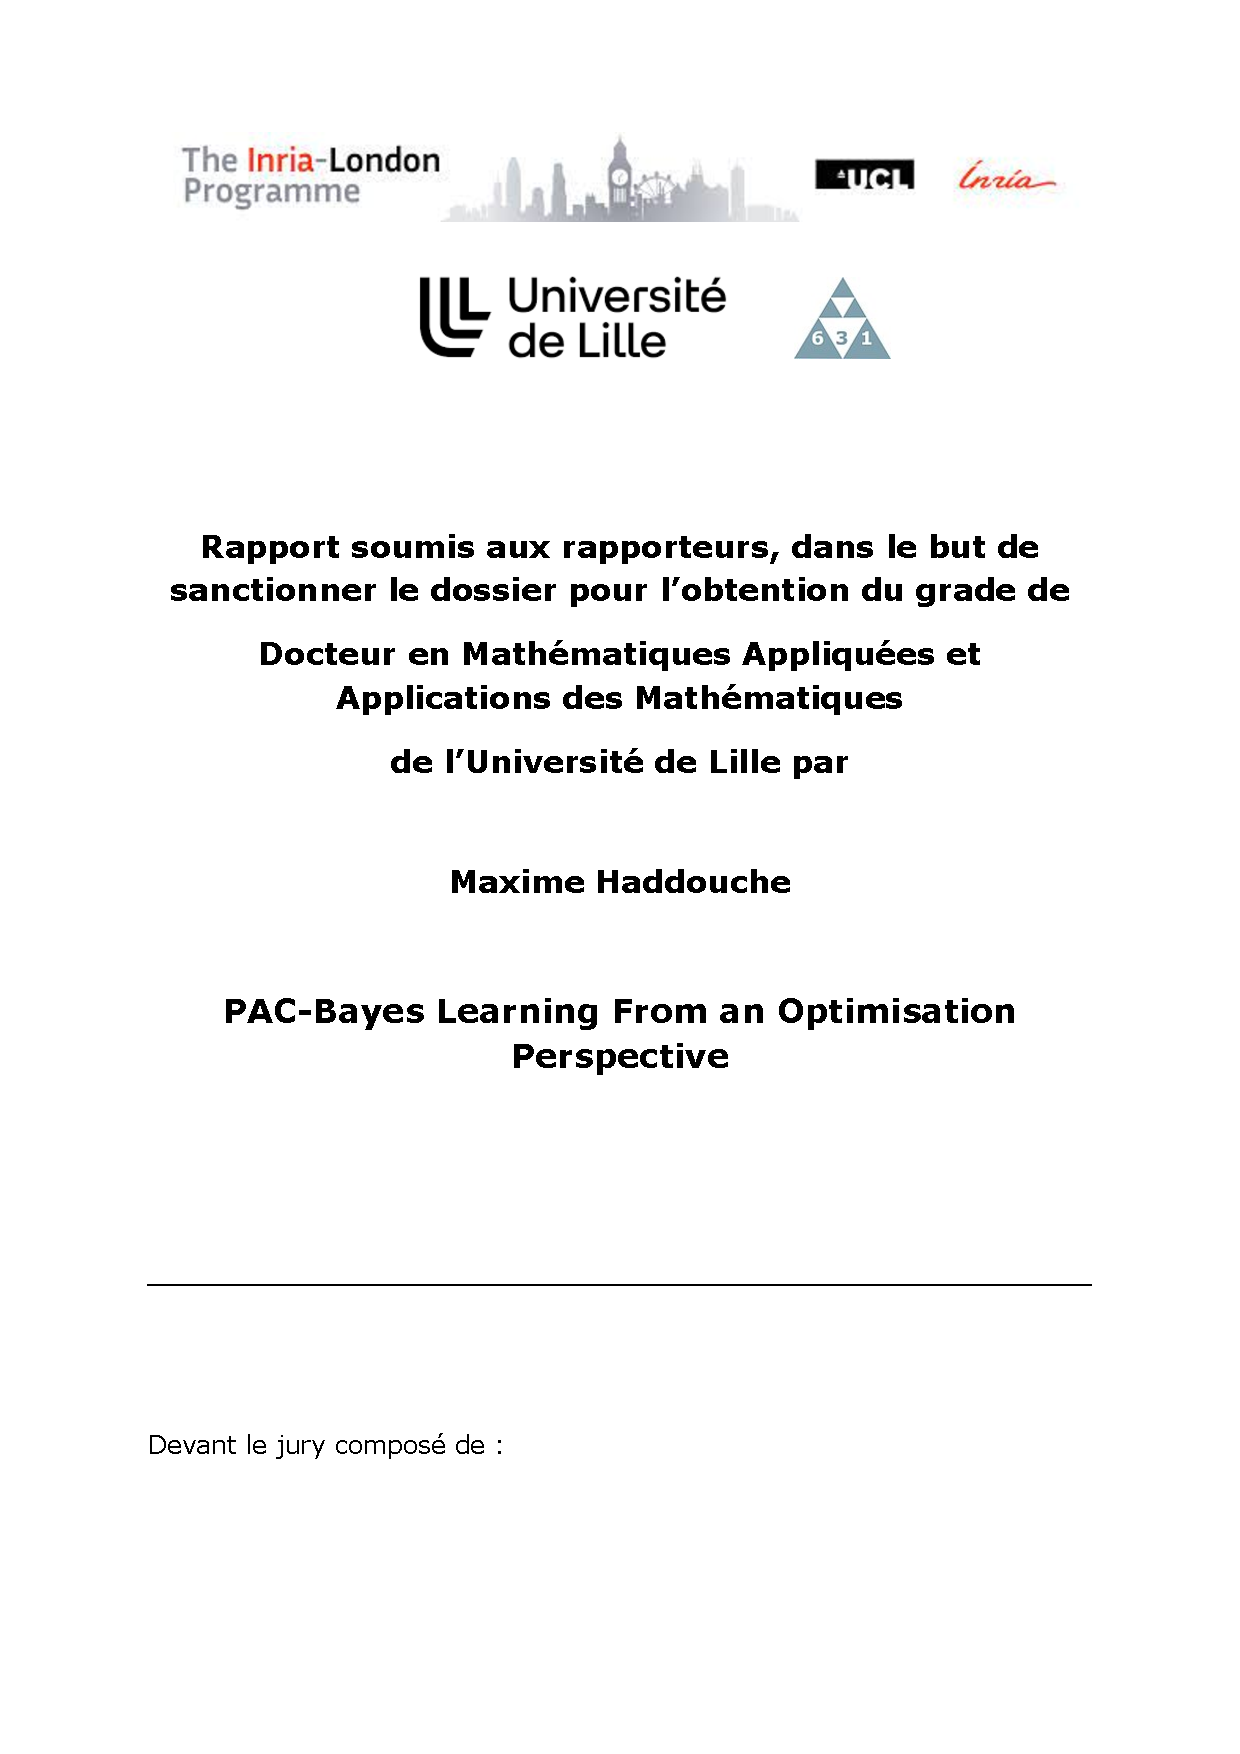
\includepdf{main/begin.pdf}

% ----------------------------------------------------------------------------------------------- %

\section*{Remerciements}

Ces quelques lignes viennent d'un matin de juillet qui parachève l'écriture de ce manuscrit, produit d'un voyage rarement hésitant mais toujours incertain. Le soleil se lève, abreuvant de ses rayons un bosquet de noms toujours croissant et impatient d'arriver au plus vite sur le papier pour faire fleurir sur vos lèvres, lecteurs et lectrices, le coin d'un sourire. 
Une métaphore en guise de commencement: cette thèse est une lance finement ouvragée, je n'en suis que le modeste fer, sobre et discret qui s'attêle à la tâche, là où vous tous formez cette hampe magnifique qui donne prestance, extension et force.\\
Commençons par la prestance, toute scientifique, de ce manuscrit qui n'aurait pu être sans Benjamin, qui m'a accompagné pendant quatre ans et qui m'a appris les divers aspect du métier et m'a fait évoluer d'étudiant enthousiaste à docteur en herbe. Un merci particulier pour m'avoir laissé bricoler mon cadre de vie insolite à Paris qui, pour mes proches, m'a maintenu loin du labo. Tout autre  Un grand merci également à Umut Simsekli, Paul Viallard, Pierre Jobic, Omar Rivasplata ainsi que John Shawe-Taylor pour m'avoir fait découvrir, sous divers aspects, la richesse de la collaboration qui offre un sens bien plus humain aux choses de la science. Point d'orgue sur cette liste déjà fournie, un grand merci aux membres du jury, Stéphane Chrétien qui a eu la gentillesse de s'intéresser à mes travaux il y a déja quelques mois, Claire Boyer et Gérard Biau que j'ai connu en temps qu'enseignants à Jussieu aux prémisses de ma thèse et dont la présence dans ce comité clôt magnifiquement cette boucle. Enfin, un grand merci à Frédéric Chazal et Pascal Germain d'être rapporteur et d'avoir consacré leur précieux temps à cette production scientifique qui je l'espère, aura suscité un certain interêt (et avec un peu de chance, un interêt certain).\\
Continuons par l'extension, toute spirituelle, qui m'a été prodiguée lors de cette histoire par mes amies et amis qui m'enrichissent autant qu'ils me font rire chaque jour durant, sans la merveilleuse mosaïque de leurs passions et reflexions, nul doute que ma thèse serait restée une coquille vide et sans passion. Je songe à ce magicien d'Anatole, à Anaïs qui chante à Pierre qui apparaît une deuxième fois dans ces remerciements, à Antoine qui aime trop Grenoble pour que je le voie souvent, à Farf qui a troqué la pizza cachanaise pour l'italienne? Je songe à mes amis qui dansent, tous membres la Guillotine (nom à redéfinir au demeurant): Keko et Chanus qui secrètement adorent me voir parler du grand capital, Kaou, Selene, Vince, Antoine, Juliette, Abou, Calvin, Bertrand. Merci également à Jadou et Phil qui se déhanchent comme jamais quand je joue, et dont je sais la présence, même si je ne vous vois que peu ces temps-ci, merci à Miles pour ta vision de la guitare qui a résonné à la mienne et l'a faconnée. A tous, merci pour votre musique. 

\begin{vplace}[0.7]

\setlength{\epigraphwidth}{0.72\textwidth}

\epigraph{The further backward you look, the further forward you can see.}{\textsc{Winston Churchill}}

\vspace{1cm}

\epigraph{Science is a bit like the joke about the drunk who is looking under a lamppost for a key that he has lost on the other side of the street, because that's where the light is. It has no other choice.}{\textsc{Noam Chomsky}}


\end{vplace}

% ----------------------------------------------------------------------------------------------- %

\dominitoc

\tableofcontents
\newpage
\listoffigures
\newpage
\listofalgorithms
\newpage
\listoftheorems

\newcommand{\wbf}{\mathbf{w}}
\newcommand{\Wbf}{\mathbf{W}}
\newcommand{\xbf}{\ensuremath{\mathbf{x}}}
\newcommand{\zbf}{\ensuremath{\mathbf{z}}}
\newcommand{\zerobf}{\mathbf{0}}
\newcommand{\h}{h}
\newcommand{\dist}{\mathrm{dist}}

\newcommand{\Acal}{\ensuremath{\mathcal{A}}}
\newcommand{\Bcal}{\ensuremath{\mathcal{B}}}
\newcommand{\Ccal}{\ensuremath{\mathcal{C}}}
\newcommand{\Dcal}{\ensuremath{\mathcal{D}}}
\newcommand{\Fcal}{\ensuremath{\mathcal{F}}}
\newcommand{\Hcal}{\ensuremath{\mathcal{H}}}
\newcommand{\Mcal}{\ensuremath{\mathcal{M}}}
\newcommand{\Ncal}{\ensuremath{\mathcal{N}}}
\newcommand{\Pcal}{\ensuremath{\mathcal{P}}}
\newcommand{\Scal}{\ensuremath{\mathcal{S}}}
\newcommand{\Tcal}{\ensuremath{\mathcal{T}}}
\newcommand{\Xcal}{\ensuremath{\mathcal{X}}}
\newcommand{\Ycal}{\ensuremath{\mathcal{Y}}}
\newcommand{\Zcal}{\ensuremath{\mathcal{Z}}}

\newcommand{\Ebb}{\ensuremath{\mathbb{E}}}
\newcommand{\Pbb}{\ensuremath{\mathbb{P}}}
\newcommand{\Rbb}{\ensuremath{\mathbb{R}}}
\newcommand{\Nbb}{\ensuremath{\mathbb{N}}}

\newcommand{\Rfrak}{\ensuremath{\mathfrak{R}}}

\newcommand{\RA}{\right\rangle}
\newcommand{\LA}{\left\langle}
\newcommand{\LB}{\left[}
\newcommand{\RB}{\right]}
\newcommand{\LC}{\left\{}
\newcommand{\LM}{\left\|}
\newcommand{\RM}{\right\|}
%\newcommand{\RC}{\right\}}
%\newcommand{\RN}{\right\vert}
\newcommand{\LN}{\left\vert}
\newcommand{\LP}{\left(}
\newcommand{\RP}{\right)}

\newcommand{\wrt}{{\it w.r.t.}\xspace}
\newcommand{\eg}{{\it e.g.}\xspace}
\newcommand{\ie}{{\it i.e.}\xspace}
\newcommand{\iid}{{\it i.i.d.}\xspace}

\newcommand{\defeq}{:=}

\DeclareMathOperator*{\EE}{\Ebb}
\DeclareMathOperator*{\PP}{\Pbb}
\DeclareMathOperator*{\argmin}{\mathrm{argmin}}
\DeclareMathOperator*{\vect}{\mathrm{vec}}
\DeclareMathOperator*{\leaky}{\mathrm{Leaky}}
\DeclareMathOperator*{\proj}{\mathrm{Proj}}

\newcommand{\Irm}{\mathrm{I}}
\newcommand{\KL}{\mathrm{KL}}
\newcommand{\KLr}{\overline{\KL}}
\newcommand{\Hell}{H^2}
\newcommand{\TV}{TV}
\newcommand{\kl}{\mathrm{kl}}
\newcommand{\W}{\mathrm{W}}
\newcommand{\Lip}{\mathrm{Lip}}

\newcommand{\D}{\Dcal}
\newcommand{\Dm}{\Dcal_{m}}
\renewcommand{\H}{\Hcal}
\newcommand{\Hb}{\overline{\Hcal}}
\newcommand{\loss}{\ell}
\renewcommand{\P}{\mathrm{P}}
\newcommand{\Q}{\mathrm{Q}}
\newcommand{\R}{\Rbb}
\newcommand{\N}{\Nbb}
\renewcommand{\S}{\Scal}
\newcommand{\Sm}{\S_m}
\newcommand{\Risk}{\text{R}}
\newcommand{\Riskhat}{\hat{\Risk}}
\newcommand{\X}{\Xcal}
\newcommand{\x}{\xbf}
\newcommand{\y}{y}
\newcommand{\Y}{\Ycal}
\newcommand{\Z}{\Zcal}
\newcommand{\z}{\zbf}
\newcommand{\varepsilonbf}{\boldsymbol{\varepsilon}}
\newcommand{\rad}{\mathdbcal{E}}
\newcommand{\DS}{\D_\S}
\newcommand{\yeast}{{\sc Yeast}\xspace}
\newcommand{\phishing}{{\sc Phishing}\xspace}
\newcommand{\mushrooms}{{\sc Mushrooms}\xspace}
\newcommand{\mnist}{{\sc MNIST}\xspace}
\newcommand{\fashion}{{\sc FashionMNIST}\xspace}
\newcommand{\indic}{\mathds{1}}

\newcommand{\OPBTest}{\normalfont\textsc{OPBTest} }
\newcommand{\OPBTrain}{\normalfont\textsc{OPBTrain} }

\newcommand{\Vhat}{\hat{V}}
\newcommand{\Bhat}{\hat{B}}
\DeclareMathOperator*{\ReLU}{\mathrm{ReLU}}

\newcommand{\Cfrak}{\ensuremath{\mathfrak{C}}}

\newcommand{\Poinc}{\texttt{Poinc}}
\newcommand{\Lsob}{\texttt{L-Sob}}
\newcommand{\Ent}{\mathrm{Ent}}
\newcommand{\Var}{\mathrm{Var}}
\DeclareMathOperator*{\Err}{\mathrm{Err}}


\let\oldQ\Q
\let\oldP\P
\renewcommand{\Q}{\orange{\oldQ}}
\renewcommand{\P}{\green{\oldP}}


% ----------------------------------------------------------------------------------------------- %

\let\proof\newproof
\let\endproof\endnewproof
 
% ----------------------------------------------------------------------------------------------- %
\counterwithout{figure}{section}
%\documentclass{standalone}
\usepackage{tikz}
\usepackage{xcolor}
\usepackage{amssymb}
\usepackage{amsmath}
\usepackage{amsfonts}
\usepackage{mathtools}
\usepackage{xspace}
\usepackage{stmaryrd}
\usepackage[misc]{ifsym}
\usepackage{bbold}
\usepackage{etoolbox}

\usepackage[LGR,OT1]{fontenc}
\usepackage[utf8]{inputenc}

\ifcsundef{abf}{\newcommand{\wbf}{\mathbf{w}}
\newcommand{\Wbf}{\mathbf{W}}
\newcommand{\xbf}{\ensuremath{\mathbf{x}}}
\newcommand{\zbf}{\ensuremath{\mathbf{z}}}
\newcommand{\zerobf}{\mathbf{0}}
\newcommand{\h}{h}
\newcommand{\dist}{\mathrm{dist}}

\newcommand{\Acal}{\ensuremath{\mathcal{A}}}
\newcommand{\Bcal}{\ensuremath{\mathcal{B}}}
\newcommand{\Ccal}{\ensuremath{\mathcal{C}}}
\newcommand{\Dcal}{\ensuremath{\mathcal{D}}}
\newcommand{\Fcal}{\ensuremath{\mathcal{F}}}
\newcommand{\Hcal}{\ensuremath{\mathcal{H}}}
\newcommand{\Mcal}{\ensuremath{\mathcal{M}}}
\newcommand{\Ncal}{\ensuremath{\mathcal{N}}}
\newcommand{\Pcal}{\ensuremath{\mathcal{P}}}
\newcommand{\Scal}{\ensuremath{\mathcal{S}}}
\newcommand{\Tcal}{\ensuremath{\mathcal{T}}}
\newcommand{\Xcal}{\ensuremath{\mathcal{X}}}
\newcommand{\Ycal}{\ensuremath{\mathcal{Y}}}
\newcommand{\Zcal}{\ensuremath{\mathcal{Z}}}

\newcommand{\Ebb}{\ensuremath{\mathbb{E}}}
\newcommand{\Pbb}{\ensuremath{\mathbb{P}}}
\newcommand{\Rbb}{\ensuremath{\mathbb{R}}}
\newcommand{\Nbb}{\ensuremath{\mathbb{N}}}

\newcommand{\Rfrak}{\ensuremath{\mathfrak{R}}}

\newcommand{\RA}{\right\rangle}
\newcommand{\LA}{\left\langle}
\newcommand{\LB}{\left[}
\newcommand{\RB}{\right]}
\newcommand{\LC}{\left\{}
\newcommand{\LM}{\left\|}
\newcommand{\RM}{\right\|}
%\newcommand{\RC}{\right\}}
%\newcommand{\RN}{\right\vert}
\newcommand{\LN}{\left\vert}
\newcommand{\LP}{\left(}
\newcommand{\RP}{\right)}

\newcommand{\wrt}{{\it w.r.t.}\xspace}
\newcommand{\eg}{{\it e.g.}\xspace}
\newcommand{\ie}{{\it i.e.}\xspace}
\newcommand{\iid}{{\it i.i.d.}\xspace}

\newcommand{\defeq}{:=}

\DeclareMathOperator*{\EE}{\Ebb}
\DeclareMathOperator*{\PP}{\Pbb}
\DeclareMathOperator*{\argmin}{\mathrm{argmin}}
\DeclareMathOperator*{\vect}{\mathrm{vec}}
\DeclareMathOperator*{\leaky}{\mathrm{Leaky}}
\DeclareMathOperator*{\proj}{\mathrm{Proj}}

\newcommand{\Irm}{\mathrm{I}}
\newcommand{\KL}{\mathrm{KL}}
\newcommand{\KLr}{\overline{\KL}}
\newcommand{\Hell}{H^2}
\newcommand{\TV}{TV}
\newcommand{\kl}{\mathrm{kl}}
\newcommand{\W}{\mathrm{W}}
\newcommand{\Lip}{\mathrm{Lip}}

\newcommand{\D}{\Dcal}
\newcommand{\Dm}{\Dcal_{m}}
\renewcommand{\H}{\Hcal}
\newcommand{\Hb}{\overline{\Hcal}}
\newcommand{\loss}{\ell}
\renewcommand{\P}{\mathrm{P}}
\newcommand{\Q}{\mathrm{Q}}
\newcommand{\R}{\Rbb}
\newcommand{\N}{\Nbb}
\renewcommand{\S}{\Scal}
\newcommand{\Sm}{\S_m}
\newcommand{\Risk}{\text{R}}
\newcommand{\Riskhat}{\hat{\Risk}}
\newcommand{\X}{\Xcal}
\newcommand{\x}{\xbf}
\newcommand{\y}{y}
\newcommand{\Y}{\Ycal}
\newcommand{\Z}{\Zcal}
\newcommand{\z}{\zbf}
\newcommand{\varepsilonbf}{\boldsymbol{\varepsilon}}
\newcommand{\rad}{\mathdbcal{E}}
\newcommand{\DS}{\D_\S}
\newcommand{\yeast}{{\sc Yeast}\xspace}
\newcommand{\phishing}{{\sc Phishing}\xspace}
\newcommand{\mushrooms}{{\sc Mushrooms}\xspace}
\newcommand{\mnist}{{\sc MNIST}\xspace}
\newcommand{\fashion}{{\sc FashionMNIST}\xspace}
\newcommand{\indic}{\mathds{1}}

\newcommand{\OPBTest}{\normalfont\textsc{OPBTest} }
\newcommand{\OPBTrain}{\normalfont\textsc{OPBTrain} }

\newcommand{\Vhat}{\hat{V}}
\newcommand{\Bhat}{\hat{B}}
\DeclareMathOperator*{\ReLU}{\mathrm{ReLU}}

\newcommand{\Cfrak}{\ensuremath{\mathfrak{C}}}

\newcommand{\Poinc}{\texttt{Poinc}}
\newcommand{\Lsob}{\texttt{L-Sob}}
\newcommand{\Ent}{\mathrm{Ent}}
\newcommand{\Var}{\mathrm{Var}}
\DeclareMathOperator*{\Err}{\mathrm{Err}}


\let\oldQ\Q
\let\oldP\P
\renewcommand{\Q}{\orange{\oldQ}}
\renewcommand{\P}{\green{\oldP}}
}{}
%
%%%%%%%%%%%%%%%%%%%%%%%%%%%%%%%%%%%%%%%%%%%%%%%%%%%%%%%%%%%%%%%%%%%%%%%%%%%%%%%
% font option
\renewcommand*\familydefault{\sfdefault}
\DeclareMathAlphabet{\mathgtt}{LGR}{cmtt}{m}{n}

%%%%%%%%%%%%%%%%%%%%%%%%%%%%%%%%%%%%%%%%%%%%%%%%%%%%%%%%%%%%%%%%%%%%%%%%%%%%%%%
% xcolor options

% Paul Tol's  "Vibrant" color scheme
% https://personal.sron.nl/~pault/data/colourschemes.pdf
\definecolor{blue}{HTML}{0077BB}
\definecolor{cyan}{HTML}{33BBEE}
\definecolor{green}{HTML}{009988}
\definecolor{orange}{HTML}{EE7733}
\definecolor{red}{HTML}{CC3311}
\definecolor{magenta}{HTML}{EE3377}
\definecolor{grey}{HTML}{BBBBBB}

%%%%%%%%%%%%%%%%%%%%%%%%%%%%%%%%%%%%%%%%%%%%%%%%%%%%%%%%%%%%%%%%%%%%%%%%%%%%%%%


\begin{document}
  \begin{tikzpicture}
    
  \begin{scope}[xshift=0cm, yshift=0cm]
  \node[] at (0.0,0.0) {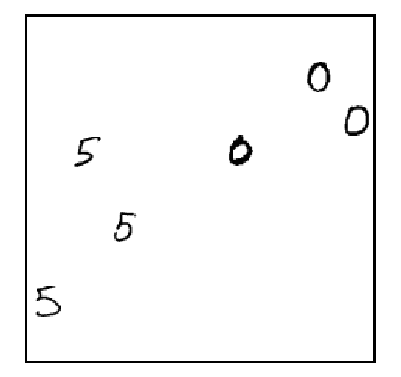
\includegraphics[scale=0.4]{chapter_1/figures/introduction_1.pdf}};  
  \end{scope}
    
  \begin{scope}[xshift=5.4cm, yshift=0cm]
  \node[] at (0.0,0.0) {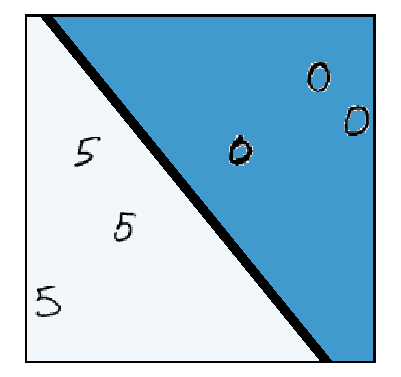
\includegraphics[scale=0.4]{chapter_1/figures/introduction_2.pdf}};  
  \end{scope}
  
  \draw [->,line width=0.05cm] (1.25, 0.0) to (4.15,0);
  \node[] at (2.7, 0.2) {{\tiny Learning}};
  
  \iffalse
  \begin{scope}[xshift=0.0cm, yshift=0.0cm]
  \draw[line width=0.1cm] (0.7, 2.83) circle (0.765cm);
    
  
  \draw[] (-1.0, 1.5) node[] {$\X{\times}\Y$};
  \clip (0,2.8) circle (1.5cm);
  \draw[step=1cm, rotate=45, black] (0.0, 0.0) grid (4, 4);
  \begin{scope}[xshift=0.7cm, yshift=-0.72cm]
  \filldraw [black, line width=0.1mm, fill=red] (0,3.65) circle (1pt) node[scale=0.5, xshift=0.6cm] {$(\x, \y)$};
  \filldraw [black, line width=0.1mm, fill=blue] (0.3,3.3) circle (1pt) node[scale=0.5, xshift=-0.7cm] {$(\x', \y')$};
  \node[scale=0.5] at (-0.52, 3.53) {$\Z_i$};
  \end{scope}
  \end{scope}
  \fi
  
  
\end{tikzpicture}
\end{document}
\counterwithin{figure}{chapter}

\newrefcontext[sorting=ydnt]
\chapter*{List of Publications}\addcontentsline{toc}{chapter}{List of Publications}
\begin{refsection}[publications.bib]
\nocite{*}
\printbibliography[heading={subbibliography}, keyword={conference}, title={International Conference}]
\printbibliography[heading={subbibliography}, keyword={workshop}, title={International Workshop}]
\printbibliography[heading={subbibliography}, keyword={nat-conference}, title={National Conference}]
\printbibliography[heading={subbibliography}, keyword={report}, title={Research Report}]
\end{refsection}

\adjustmtc[4]

% ----------------------------------------------------------------------------------------------- %
\pagestyle{headings}

\part{Background}
\label{part:background}

%\chapter[PAC-Bayes Learning, a field of many paradigms]{PAC-Bayes Learning, a field of many paradigms}
\label{chap:intro-pac-bayes}

\minitoc

\addchapterlof
\addchapterloa
\addchapterloe

\section{A brief introduction to statistical learning}
\label{sec: intro-stat-learning}
Statistical learning \citep{vapnik1999overview,james2013introduction} quantifies and identifies how learning algorithms, trained on a specific task using a finite training dataset, generalise to novel, unseen datum. More precisely, a learning agent has to learn how to answer a question, formalised as a \emph{learning problem} being a tuple $(\H,\Z,\ell)$ composed of a \emph{predictor space} on which evolves the agent during the learning process, a \emph{data space} $\Z$ and a \emph{loss function} being the mathematical formulation of the question. Such a minimalistic structure is convenient to encompass a broad range of real-life learning scenarii. To learn, the agent has access to a \emph{training dataset} $\S_m= (\z_i)_{i=1\cdots m}$. The most classical way to learn from $\Sm$ is the empirical risk minimisation (ERM), minimising the \emph{empirical risk} $\Riskhat_{\Sm}:= \frac{1}{m} \sum_{i=1}^m \ell(h,\z_i)$. In this setting, when $\S_m$ is \iid (following the distribution $\D$), two facets of generalisation are commonly studied in statistical learning for a given agent $h\in\H$.

\begin{itemize}
    \item First, the \emph{population risk} $\Risk_\D(h):= \mathbb{E}_{\z\sim\D}[\ell(h,\z)]$ focus on the average performance of our learning agent \wrt any new situation $\z\in\D$, independent of $\S_m$, possibly faced by the agent. A small population risk ensure then efficient generalisation.   
    \item Second, the \emph{generalisation gap}  $\Delta_{\Sm}(h):= \Risk_D(h) - \Riskhat_{\Sm}(h)$ evaluate the coherence between the empirical risk and the population one. Having a small generalisation gap ensure that the generalisation ability of the agent has the same magnitude than its training performance. 
\end{itemize}
Note that the population risk is a stronger notion of generalisation than the generalisation gap. However, a small generalisation gap (in absolute value) as well as a small empirical risk is enough to ensure a good population risk. Given that modern optimisation algorithm are often enough to ensure a small empirical risk, the generalisation gap has received a particular attention in statistical learning. 

\paragraph{Generalisation bounds.} Generalisation bounds are inequalities often controlling the generalisation gap by various quantities depending either on $\H,\Z$ or $\S_m$. We propose below general patterns usually involved in generalisation bounds for an agent $h_{\Sm}\in\H$ depending on $\S_m$ (for instance the output of the ERM). 

\textbf{Expected generalisation bound.} For any training set $\S_m$:

\begin{align} 
  \label{eq: expected-bound}
  \mathbb{E}_{\S_m}\LB \Delta_{\Sm}(h_{\Sm}) \RB \leq f\LP \textsc{Complexity}, \frac{1}{m}\RP. 
\end{align}

\textbf{High-probability generalisation bounds.} For any training set $\S_m$, with probability $1-\delta$ pver the draw of $\Sm$:
\begin{align}
  \label{eq: hp-bound}
  \Delta_{\Sm}(h_{\Sm}) \leq f\LP \textsc{Complexity}, \frac{1}{m}, \log\frac{1}{\delta}\RP.
\end{align}
The nature of $f$ and the \textsc{Complexity} term depend on the facet of the complexity of the learning problem we aim to focus. Celebrated examples are for instance the dimension of $\H$, if euclidean, the VC dimension of $\H$ \citep{vapnik2000learning}, the Rademacher complexity \citep{bartlett2001rademacher,bartlett2002rademacher},  the stability parameter of a learning algorithm \citep{bousquet2000algo} or the subgaussian diameter of $\Z$ \citep{kontorovich2014conc}. 
Another approach relies on the Bayesian learning paradigm, deriving \emph{posterior} knowledge from data and prior modelling of the environment. 
Then, the \textsc{Complexity} can be borrowed from information theory \citep{cover2001elements}, \eg mutual information \citep{neal2012bayesian}, or from optimal transport, \eg Wasserstein distances \citep{wang2019information,rodriguez2021tighter}. 

Those two approaches have various benefits. A notable strength of expected bounds is that they may reach fast convergence rates (\ie faster than $\frac{1}{\sqrt{m}}$) contrary to high-probability one, even when $\H$ is a singleton thanks to the central limit theorem \citep{grunwald2021mac}. However, expected bounds often involves a theoretical \textsc{Complexity} which cannot be estimated in practice and may be hard to interpret while high probability bounds may be fully empirical and can be considered with small confidence parameter $\delta$ as it is attenuated by a logarithm.

\paragraph{How to choose the complexity term ? An introductory example.} There is no evidence proving that a certain notion of complexity is preferrable to another. The choice of \textsc{Complexity} may however be driven by practical considerations, emerging from the learning problem of interest. To illustrate this point, let us focus on the following example, providing two learning problems which differs only from the predictor space $\H$ and which have very different interactions with the VC dimension.
\begin{example}
  \label{ex: neural_net}
  Consider a supervised learning problem where $\Z = \Rbb^k\times\Ycal$ with $\Ycal=\{0,1\}$, $k$ smaller than $m$ and with loss $\ell(h,(x,y))= \mathds{1}\{h(x) \neq y\}$.  First, assume that $\Hcal$ is the set of linear classifiers; \ie $\H_1:= \left\{ h_{\theta}(x)= sgn(\langle \theta,x\rangle)  \right\}$, where $sgn(a)$ denotes the sign of $a$. In this case, using the VC dimension may lead to non-vacuous generalisation bounds \citep{vapnik2000learning}. 

However, in modern machine learning, deep neural networks are often considered, let us first define a celebrated class of deep neural networks. 

\begin{definition}
    \label{def:mlp}
    A multlayer perceptron with depth $K$ and architecture $\{N_1,\cdots,N_K\}$, denoted as $h_{\wbf}(\x) \defeq Wh^{K}(\cdots h^{1}(\x))+b$, is composed of $K$ layers $h^1(\cdot),\dots,h^K(\cdot)$.
 $W\in\R^{|\Ycal|\times N_K}$ and $b\in\R^{N_K}$ are the weight matrix and the bias of the last layer, and the $i$-th layer $h^{i}$, composed of $N_i$ nodes, is defined by $h^{i}(\xbf)\defeq\sigma_i(W_i \xbf + b_i)$, where $W_i\in\R^{N_i\times N_{i-1}}$ and the bias $b_i\in \R^{N_i}$ are its weight matrix and bias respectively; $\sigma_i : \R^{N_i} \to \R^{N_i} $ is an activation function.
The weights $\wbf=\vect(\{W, W_{K}, \dots, W_1, b, b_{K}, \dots, b_1\})$ represent the vectorisation of all parameters of the network.
\end{definition}
Now, consider the learning problem with the same $\Z,\ell$ as above, but with $\H_2$ being the set of multilayer perceptrons \wrt a fixed depth $K$ and architecture $\{N_1,\cdots,N_K\}$. To be consistent with modern practice, assume also that we are in the \emph{overparametrised setting}, meaning that the space $\H_2$ has a dimension $d$ far greater than $m$.
In this case, VC dimension fails to explain the good generalisation ability (seen in practice) of multilayer perceptrons \citep{bartlett2003vapnik}.
\end{example}

Understanding the generalisation ability of deep neural networks remains nowadays a major challenge and in what follows, we focus on a modern branch of learning theory which provided non-vacuous bounds of the generalisation ability of deep neural networks: PAC-Bayes learning.

\section{An information-theoretic exposition of PAC-Bayes learning}

PAC-Bayes learning is a recent branch of learning theory which emerged in the late 90s via the seminal work of \citep{shawe1997pac,mcallester1998some,mcallester1999pac,mcallester2003pac} and later pursued by \citep{catoni2003pac,catoni2007pac}. Modern surveys recently emerged to describe the various advances in the field \citep{guedj2019primer,hellstrom2023generalization,alquier2024user}.  Similarly to the various subfields of statistical learning described in \Cref{sec: intro-stat-learning}, PAC-Bayes theory is designed top provide generalisation bounds involving a \textsc{Complexity} term apprehending a facet of the complexity of the learning problem. In PAC-Bayes, this term is inspired from the Bayesian learning paradigm of designing a \emph{posterior} knowledge of the learning problem based on the positive impact of data onto a \emph{prior} knowledge of the considered situation. A concrete example of Bayesian learning would be an explorer mapping an ill-known territory. The explorer has to adapt the existing maps at its disposal before exploration to its discoveries, generating a new map imbricating the benefits of both the prior one alongside its findings. From a mathematical perspective, the Bayes approach relies on the Bayes formula, providing an update recipe from a prior distribution $\P\in\Mcal(\Hcal)$ over the predictor space $\H$ to a posterior $\Q\in\Mcal(\Hcal)$ through a likelihood. On the contrary, PAC-Bayes, while inspired from the Bayesian philosophy, does not relies on the Bayes formula but instead on tools from information theory. This general approach benefits from additional flexibility as PAC-Bayes can be linked and applied to Bayesian learning (see \citealp{guedj2019primer}) but also blurs the notion of prior and posterior distributions, now independent of the fundamental Bayes formula. We further develop those points through two celebrated bounds: the McAllester and Catoni ones. 

\subsection*{Two fundamental results}
    The McAllester's bound \citep{mcallester2003pac} enriched with Maurer's trick \citep{maurer2004note} and Catoni's bound (\citealp[Theorem 4.1]{alquier2016properties}, being a relaxation of \citealp[Theorem 1.2.6]{catoni2007pac}) are probably the most known high-probability PAC-Bayes bounds. We recall them in \Cref{prop: mcall-catoni}.

    \begin{proposition}
        \label{prop: mcall-catoni}
        Assume $\Sm$ to be \iid.\\
    \textbf{McAllester's bound, \citep[Theorem 5]{maurer2004note}.}  For any $\delta\in(0,1),\ell\in[0,1]$, any data-free prior $\P\in\Mcal(\Hcal)$, with probability at least $1-\delta$, for any posterior $\Q\in\Mcal(\H)$,
    \begin{align}
    \label{eq: mcallester}
     \Delta_{\Sm}(\Q) \le \sqrt{\frac{\KL(\Q,\P) + \ln{\frac{2\sqrt{m}}{\delta}}}{2m}}.
    \end{align}

    \textbf{Catoni's bound, \citep[Theorem 4.1]{alquier2016properties}.}
    For any $\lambda\in\mathbb{R}/\{0\},\delta\in(0,1),\ell$ being $\sigma^2$-subgaussian and a data-free prior $\P$, with probability at least $1-\delta$ over $\S$, for any $\Q\in \Mcal(\Hcal)$,

  \begin{align}
    \label{eq: catoni}
    \Delta_{\Sm}(\Q) \leq  \frac{\KL(\Q,\P) + \log(1/\delta)}{\lambda} + \frac{\lambda\sigma^2}{2m}.  
  \end{align}

    For both results, $\Delta_{\Sm}(\Q)$ denotes the expected generalisation gap \wrt $\Q$ and $\KL$ denotes the Kullback-Leibler divergence.
    \end{proposition}

Recall that a random variable $X$ is $\sigma^2$-subgaussian if for any $\lambda\in\Rbb$, $\Ebb[\exp(\lambda(X-\Ebb[X]))] \leq \exp\LP \frac{\lambda^2 \sigma^2}{2} \RP$ and that any loss $\loss\in[0,C]$ is $C$-subgaussian. Both McAllester and Catoni bounds fit the general shape of \eqref{eq: hp-bound}. In both cases, $\textsc{Complexity}= \KL(\Q,\P)$ and $f$ varies. The immediate link with the Bayesian philosophy of learning is that the prior has to be data-free. However, \eqref{eq: mcallester} and \eqref{eq: catoni} are both valid simultaneously for any posterior, which is strictly more general than considering the Bayesian posterior. Note that if $\lambda$ is optimised, then Catoni's bound would boil down to an upgraded McAllester bound without the $\log(\sqrt{m})$ term, but such an optimisation is not feasible as $\lambda$ has to be chosen independently of the dataset $\Sm$. 
Note that this gap has been recently filled by \citet[Theorem 33]{dupuis2024generalization}. While the theoretical links between those two bounds are clear, they involve two different toolboxes: McAllester's bound heavily relies on the KL divergence between Bernoullis alongisde calculation tricks exploiting the boundedness of the loss while the original Catoni's bound \citep[Theorem 1.2.6]{catoni2007pac} exploits tools from statistical physics. 
The relaxation \eqref{eq: catoni} proposed here is reachable by a few key arguments, involved in a vast majority of PAC-Bayes proofs. We propose it below for pedagogical purpose. 

\begin{proof}[of \Cref{eq: catoni}]
Note that the first part of the proof holds for a large part of PAC-Bayes literature.
  \textbf{A generic pattern for PAC-Bayes bounds.}
    This part is designed upon two cornerstones, retrievable in many existing results: the change of measure inequality (\citealp{csizar1975divergence,donsker1976asymp} -- see also \citealp{banerjee2006bayesian,guedj2019primer} for a proof) and Markov's inequality.

  \begin{lemma}[Change of measure inequality]
    \label{l: change_meas} 
    For any measurable function $\psi :\mathcal{H}\rightarrow \mathbb{R}$ and any distributions $\Q,\P$ on $\mathcal{H}$:
    
    \[ \mathbb{E}_{h\sim \Q}[\psi (h)] \leq \operatorname{KL}(\Q,\P) + \log\left( \mathbb{E}_{h\sim \P}[\exp(\psi(h))]  \right).  \]
    \end{lemma}
For a given $\lambda>0$, the change of measure inequality is then applied to a certain function $f_m: \Hcal \mathbb{R}$, possibly involving $\Sm$: for all posteriors $Q$,
\begin{align}
\label{eq: change_meas_pacb}
\mathbb{E}_{h\sim \Q}[f_m(h)] \leq \operatorname{KL}(\Q,\P) + \log\left( \mathbb{E}_{h\sim \P}[\exp(f_m(h))]  \right).
\end{align}
To deal with the random variable  $X(\Sm):=\mathbb{E}_{h\sim \P}[\exp(f_m(h))] $, our second building block is Markov's inequality $\left(\mathbb{P}(X>a) \leq \frac{\mathbb{E}[X]}{a}\right)$ which we apply for a fixed $\delta\in (0,1)$ on $X(\Sm)$ with $a= \mathbb{E}_{\Sm}[X(\Sm)]/\delta$.
Taking the complementary event gives that for any $m$, with probability at least $1-\delta$ over the sample $\Sm$, $X(\Sm)\leq \mathbb{E}_{\Sm}[X(\Sm)]/\delta$, thus:


\begin{equation}
  \label{eq: prelim_pb_bound}
  \mathbb{E}_{h\sim \Q}[f_m(h)] \leq \operatorname{KL}(\Q,\P) + \log(1/\delta) + \log\left( \mathbb{E}_{h\sim P}\mathbb{E}_{\Sm}[\exp(f_m(h))]  \right).
\end{equation}

Note that in \eqref{eq: prelim_pb_bound}, we swapped the two expectations in the last term thanks to Fubini's theorem and the fact that $\P$ is data-free.

\textbf{Proving Catoni's bound.}
Now, we take $f_m(h)= \lambda\Delta_{\Sm}$ and consider for any $h\in\Hcal, A(h)= \mathbb{E}_{\Sm}[\exp(f_m(h))]$. 

Note that, given $\Sm$ is iid, 
\begin{align*}
  A(h) &= \prod_{i=1}^m \mathbb{E}_{\Sm}\LB\exp\LP\frac{\lambda}{m}(\Risk_\D(h)-\ell(h,\z_i))\RP\RB, 
  \intertext{and thanks to Heoffding's lemma alongside $\ell$ being $\sigma^2$-subgaussian,}
  A(h) &\leq \prod_{i=1}^m \exp\LP \frac{\lambda^2 \sigma^2}{2m^2} \RP = \exp\LP \frac{\lambda^2 \sigma^2}{2m} \RP.
\end{align*}

Plugging this upper bound in \eqref{eq: prelim_pb_bound} and dividing by $\lambda$ concludes the proof.
\end{proof}

The generic pattern \eqref{eq: prelim_pb_bound}, allows to retrieve many PAC-Bayes bounds, starting with McAllester's one, where $f_m= kl(\Risk_\D(h),\Riskhat_{\Sm}(h)), kl$ being the KL divergence between Bernoullis and completing with the subtle calculations of \citet{maurer2004note}. This pattern is also valid, for instance, for the results of \citet{germain2009pac}, the Bernstein PAC-Bayesian bounds of \citet{tolstikhin2013pac,mhammedi2019pac} and many other results, \eg \citet{thiemann2017strongly,guedj2018pac,holland2019pac,wu2022split}. This then pins two major points for a large part of PAC-Bayes literature: 

\begin{enumerate}
  \item Interpreting PAC-Bayes from a Bayesian prism is legitimated by the change of measure inequality, yet the KL divergence. More generally, this property allows interpreting PAC-Bayes under a more general information theoretic paradigm, where information from the prior is partially transferred to the posterior (here by absolute continuity to keep the KL finite). This vision encompasses the Bayesian one, while being less restrictive.
  \item The statistical properties of the learning problem are linked to the exponential moment coming from the change of measure inequality, this often implies the strong assumptions of \Cref{prop: mcall-catoni}: data-free prior, bounded or subgaussian losses (sometimes attenuated to subexponentiality \citealp{catoni2004statistical}).
\end{enumerate}

\paragraph{A theory suited for \Cref{ex: neural_net}?}
The two previous points show that \Cref{prop: mcall-catoni} holds for learning problem with light-tailed losses (often bounded), \iid data, encompassing classification tasks for instance. Then, PAC-Bayes learning seems suited to understand, on such problems, the McAllester and Catoni bounds are suited to the learning problem $(\Hcal_2,\Z,\ell)$ of \Cref{ex: neural_net}. 

However, the question of their tightness is unsolved as we do not know the behavior of the KL term in practice. Furthermore the question of which distribution $\Q$ should be taken in \Cref{prop: mcall-catoni} remains open.

% Rework this paragraph, do not talk about dziugaite now, just say that the  theoretical framework fits the learning problem of example 1.1.1. But it still needs to be verified that this complexity measure will be small for neural nets, and thus, non-vacuous bound can be attained in this case.

\section{From theory to learning algorithms}

\subsection*{Algorithms associated to McAllester and Catoni bounds}
A shared particularity of McAllester and Catoni bounds is that they are both fully empirical. Then it is possible to minimise them in practice and thus, deriving new theory-driven learning algorithms which are expected to have at worse, a small generalisation gap and at best, a small population risk. More precisely, learning algorithms associated to \Cref{prop: mcall-catoni} are stated below: 

\begin{align}
  \label{eq: alg-mcall}
  \Q_{M}:= \underset{\Q\in\mathcal{C}}{\operatorname{argmin}}\; \Riskhat_{\Sm}(\Q) + \sqrt{\frac{\KL(\Q,\P)}{2m}}.
  \intertext{For any $\lambda>0$,}
  \label{eq: alg-catoni}
  \Q_{C}:= \underset{\Q\in\mathcal{C}}{\operatorname{argmin}}\; \Riskhat_{\Sm}(\Q) +\frac{\KL(\Q,\P)}{\lambda}.
\end{align}
In both cases, $\mathcal{C}\subseteq \Mcal(\Hcal)$ is the class of distributions on which we optimise. The choice of $\mathcal{C}$ can come from a priori knowledge of the problem or from optimisation concerns to make the KL divergence tractable.  

Knowing Catoni's bound is a relaxation of McAllester's one, it seems more natural to consider $\Q_{M}$ over $\Q_{C}$. However, the presence of a square root in \eqref{eq: alg-mcall} can be challenging for practical optimisation. We illustrate this below.
\begin{example}
  \label{ex: gaussian-kl}
  Consider the case where, for a given $\sigma>0$, $\mathcal{C}= \{\Ncal(\mu,\sigma^2 \mathrm{Id}) \mid \mu\in\Rbb^d\}$. Then the for any $\P= \Ncal(\mu_1,\sigma^2 \mathrm{Id}), \Q= \Ncal(\mu_2,\sigma^2 \mathrm{Id})$, $ \KL(\Q,\P)= \frac{\|\mu_1-\mu_2\|^2}{2\sigma^2}$. 
  Then, optimising \eqref{eq: alg-mcall} in this case implies to lose the strong convexity of the KL divergence while it is retained for \eqref{eq: alg-catoni}.
\end{example}
  
Another practical advantage of \eqref{eq: alg-catoni} over \eqref{eq: alg-mcall} emerges when $\mathcal{C}= \Mcal(\Hcal)$. In this case, Catoni's bound admits a closed form solution, while McAllester's one should be numerically optimised on all the space of distributions, which is not feasible. This closed form, extracted from \citet[Section 5.1]{catoni2003pac}, is recalled below.

\begin{align}
  \label{eq: catoni-gibbs}
  \text{When}\; \mathcal{C}= \Mcal(\Hcal),\; d\Q_{C}(h) = \frac{\exp(-\lambda \Riskhat_{\Sm}(h))}{\Ebb_{h\sim\P}[\exp(-\lambda \Riskhat_{\Sm}(h))]} d\P(h)
\end{align}

Then, $\Q_{C} = \P_{-\lambda \Riskhat_{\Sm}}$ is the \emph{Gibbs posterior} associated to $\P,\lambda\Riskhat_{\Sm}$. By introducing Gibbs posterior in statistical learning, \citet{catoni2007pac} draws a theoretical link between statistical physics and learning theory. Unfortunately, Gibbs posteriors often requires Monte Carlo methods to be implemented, which can be in practice time-consuming. Below we then focus on PAC-Bayes algorithms working on a subset $\mathcal{C}$ of $\Mcal(\Hcal)$. 

\subsection*{Instantiation and efficiency of PAC-Bayesian algorithms}

\paragraph{A general pattern for PAC-Bayesian algorithms}

The introductory examples \eqref{eq: alg-mcall},\eqref{eq: alg-catoni} unveil a general design for any KL-based PAC-Bayesian algorithm. satisfy a tradeoff between \textit{(i)} the empirical risk, showing that the learner has to fit the training dataset, and \textit{(ii)} a \emph{regulariser} being a function of $\KL(\Q,\P)$. This regulariser ensures that, during training, the learner will not overfit on training data. This training ensures a good generalisation ability as long as the associated generalisation bound is small. 

We then understand better the conceptual ins and outs of PAC-Bayes algorithms, two unanswered questions remains: 

\begin{enumerate}
  \item How are those algorithms instantiated in practice?
  \item Are these algorithms efficient and do they come with non-vacuous theoretical guarantees? 
\end{enumerate}

\paragraph{Instantiating a PAC-Bayes algorithm}
  In practice, using a single prior $\P$ usually does not work but it remains theoretically possible to consider a finite set of priors. Indeed, if one wants to consider $k$ priors, then it is possible to consider $k$ PAC-Bayes bounds holding for each of those priors with probability at least $1-\frac{\delta}{k}$ and then consider a union bound, such a set of priors is called a grid. This method has been widely used in many PAC-Bayes work with clever grids, deteriorating initial bounds at the cost of supplementary $\log(n)$ or $\log\log(n)$ (divided by $m$), see \eg \citet{alquier2024user}. 
  Similarly, for Catoni-typed algorithms where a parameter $\lambda$ is involved, it is also possible to consider grids for it. In both cases, considering grids allows to optimise on both the prior, the posterior (and possibly $\lambda$ when involved) and then taking the closest value of those optimised parameters on the grid to still obtain theoretical guarantees. Another technique to ensure a good prior is to sacrifice a part of the training set to pre-train $\P$. 
  Doing so, the prior is then data-dependent and yields tighter bounds alongside increased performance \citep{perez2021tighter}.

\paragraph{Efficiency of PAC-Bayes algorithms on supervised learning problems.}
The work of \citet{dziugaite2017computing} showed that optimising \eqref{eq: alg-mcall} when $\mathcal{C}$ is a class of Gaussian measures for the weights of a deep neural network yields non-vacuous generalisation bound, meaning that the generalisation benefits of PAC-Bayesian training on deep nets can be theoretically ensured. In their work, authors used the instantiation toolbox described above, alongside a preliminary use of Stochastic Gradient Descent (SGD) to update $\Q$ before the PAC-Bayes training algorithm. This promising work paved the way to various extensions, providing non-vacuous guarantees for a wide range PAC-Bayes algorithms \citep{rivasplata2019pac,letarte2019dichotomize,perezortiz2021learning,perez2021progress,perez2021tighter,dziugaite2021role,biggs2022non,biggs2023tighter}, showing that the PAC-Bayes toolbox provides elements of answer to understand the generalisation ability of neural networks. Beyond generalisation guarantees, PAC-Bayes bounds may also be useful to propose original training methods, even if the associated guarantees are vacuous \citep{biggs2021differentiable,biggs2022margin}. Another important empirical use is to exploit PAC-Bayes bounds as correlation measures, to see whether a decrease of the bound is related to an increased generalisation ability of the learner. For instance \citet{neyshabur2017explor} used McAllester's bound \eqref{eq: mcallester} as a 'flatness' measure and showed that it correlates well with a good generalisation ability for a few learning problems. This conclusion has been extended to a wider range of problems in \citet{jiang2020fantastic,dziugaite2020search}. 
\\
\paragraph{PAC-Bayes algorithms beyond supervised learning.} While supervised learning is a widely used setting to perform experiments in PAC-Bayes learning (often involving celebrated datasets such as MNIST or CIFAR-10), the McAllester bound holds for any learning problem with bounded loss, going beyond this setting. This theoretical flexibility has been exploited to derive PAC-Bayesian algorithm for various learning settings reinforcement learning \citep{fard2010pac}, multi-armed bandits \citep{seldin2011pac,seldin2012pac,sakhi2023pac}, meta-learning \citep{amit2018meta,farid2021generalization,rothfuss2021pacoh,rothfuss2022pac,ding2021bridging} to name but a few. 
\\
\paragraph{Is \Cref{ex: neural_net} tackled now?}
\citep{dziugaite2017computing} and following works have provided a positive answer by obtaining non-vacuous guarantees (sometimes tight) for $(\Hcal_2,\Zcal,\ell)$ of \Cref{ex: neural_net} for various $\Z$ (being, \eg, set of images for MNIST CIFAR-10 etc...). To obtain such guarantees, a PAC-Bayesian training needs to be performed to minimise its associated theoretical bound. That being said, several questions then legitimately emerge.

\begin{itemize}
  \item Modern machine learning often implies learning problems where assumptions such as bounded (or subgaussian) losses or \iid data do not hold. Is PAC-Bayes theory extendable beyond those assumptions? 
  \item As shown in \citet{dziugaite2017computing}, the PAC-Bayesian training is often combined to another procedure (\eg ERM) to yield non-vacuous bounds. However, PAC-Bayes bounds do not bring the theoretical understanding of such additional methods, often outputting deterministic predictors (\ie Dirac distributions). This kind of predictor is not allowed in \eqref{eq: mcallester}, \eqref{eq: catoni}. Is it possible to obtain PAC-Bayes bounds valid for such methods? 
\end{itemize}



\section{An optimisation perspective of PAC-Bayes}

The questions raised at the end of the previous part are important as they underline a gap between the information-theoretic approach of PAC-Bayes bounds and practical optimisation. A supplementary example of this is the grid required in practice to optimise the prior (and/or $\lambda$ in Catoni's bound). Indeed this hybrid solution is required to roughly fit theory,(exploiting a single prior) and practice (optimising freely the prior on a continuous space), while not being truly adapted to any of these settings. This then raises the following fundamental question:
\[ \textbf{Can we think PAC-Bayes learning from an optimisation perspective?} \]

The elements of answer to this question are multiple. First, one can mix PAC-Bayes argument with geometric properties of optimisation procedure to obtain generalisation bounds designed for specific algorithms exploiting their geometric properties and assumptions, including but not limited to, SGD, Langevin dynamics  \citep{london2017pac,dziugaite2018entropy,neu2021info,clerico2022generalisation,haghifam2023limit,zhou2023toward}. Those works shows both convergence properties as well as minimax rates, showing the impact of PAC-Bayes learning to provide a better theoretical understanding of the generalisation ability of concrete algorithms. 

A second approach consists in describe general principles that should be satisfied by the various terms and assumptions in PAC-Bayes when looking at this through the prism of optimisation. We propose such an analysis below.

\subsubsection*{An optimisation-driven view of PAC-Bayes}

\begin{itemize}
  \item \textbf{Statistical assumptions.} While $\ell$ satisfies desirable geometric properties (convexity, gradient lipschitz ...), no statistical assumption is needed. However, the output of two runs of a stochastic optimisation algorithm on the same training set may vary a lot.  For the specific case of SGD, many works shows that SGD exhibits a heavy-tailed behavior (see \eg \citealp{simsekli2019tail,zhang2020adaptive,gurbuzbalaban2020heavy}). Given that such heavy-tailed consideration emerges from the most celebrated algorithm, generalisation bounds, from an optimisation point of view, should hold with weak statistical assumptions on the dataset, even if additional geometric assumptions on the loss may emerge.
  \item \textbf{The role of the prior.} The information-theoretic approach justify the Bayesian view of the prior as discussed earlier. In this spirit it is also possible to sacrifice a part of the training set (\ie of the available information) to enrich $\P$ and then partially explain the efficiency of an information-theoretic training.  Those two vision are not easily linked to optimisation concerns as the first one would be linked to a 'good' initialisation, something we cannot know in advance, while the second makes little sense as $\P$ is obtained through a first, unexplained, optimisation process which is necessary to understand the efficiency of the second part of training, outputting $\Q$. From an optimisation stance, we suggest to assign only two possible roles to $\P$: \textit{(i)} the initialisation of the optimisation algorithm, then its impact should be attenuated through the learning process and \textit{(ii)} a minimiser we aim to reach through optimisation. In this case, its impact is crucial as it translates the speed of convergence of our learning algorithms.
  \item \textbf{The place of stochastic predictors.} Involving a KL divergence as a complexity brings a particular focus on stochastic predictors, drawn from a distribution $\Q$. Classical PAC-Bayes bounds usually focus on the average performance of such a predictor (hence the expectation over $\Q$ in \eqref{eq: mcallester},\eqref{eq: catoni}), but recent extensions directly proposed guarantees for a single draw over $\Q$ \citep{rivasplata2020pac,viallard2023general}. However, involving a KL implies that $\Q$ has to be absolutely continuous \wrt $\P$,  meaning that the support of $\Q$ cannot go beyond the one of $\P$: this excludes the case of Dirac distributions, \ie deterministic predictors. This is a clear limitation of the information-theoretic approach, as many learning algorithms outputs a deterministic predictor and thus, should be avoided to be in line with common practice in optimisation.
\end{itemize}

Those three points, while not necessarily considered explicitly through the lens of optimisation have been recently challenged, and modern advances are gathered below. 



\subsubsection*{PAC-Bayes beyond the usual setting}

Recall that according to what we saw in McAllester's bound \eqref{eq: mcallester} and Catoni's one \eqref{eq: catoni}, we denote by usual setting a bound holding for \iid $\Sm$, with bounded or subgaussian losses and involving a KL divergence as \textsc{Complexity} term. Many works overcame at least one of this assumption as precised below. 

\paragraph{Beyond \iid data} The work of \citet{fard2010pac} established links between reinforcement learning and PAC-Bayes theory. This naturally led to the study of PAC-Bayesian bound for martingales instead of \iid data \citep{seldin2011pac,seldin2012bandit,seldin2012pac}. Also, PAC-Bayesian bound for lifelong learning \citep{pentina2014pac,flynn2022pac} challenged also the \iid assumption. We also denote that the PAC-Bayes bound for meta learning \citep{amit2018meta,farid2021generalization,rothfuss2021pacoh,rothfuss2022pac,ding2021bridging} consider independent but non-identically distributed datasets (corresponding to different tasks).

\paragraph{Avoiding light-tailed losses.} Light-tailed losses encompass bounded, subgaussian, subexponential losses. Deriving PAC-Bayes bound for heavy-tailed losses, starting from \citet{audibert2011robust} which provided PAC-Bayes bounds for least square estimators with heavy-tailed random variables. Their results was suboptimal with respect to the intrinsic dimension and was followed by further works from \citet{catoni2016pac} and \citet{catoni2017dimension}.
More recently, this question has been addressed in the works of \citet{alquier2018simpler, holland2019pac,kuzborskij2019efron,haddouche2021pac}, extending PAC-Bayes to heavy-tailed losses under additional technical assumptions.

\paragraph{Towards data-dependent priors.} The work of \citep{catoni2007pac,lever2010distribution,lever2013tighter} proposed priors, not directly data-dependent, but depending of the data distribution $\Dcal$ when \iid data are considered. can be informed by the
data-generating distribution, \citet{parradohernandez2012pac,oneto2016pac,dziugaite2017computing,mhammedi2019pac} also obtained PAC-Bayes bound with data-dependent priors by infusing directly data in the prior (and sacrificing a part of the dataset). The drawback of this method is that, in practice, such a prior allows tighter bounds, but at the cost of a reduced theoretical understanding as the prior is in practice often learned via ERM, and the PAC-Bayes bound hardly gives insights on what happens during this pre-training. Furthermore, if this pre-training has already made the bound converge to a minimum generalising well, then the PAC-Bayes training has no effect and the associated bound is no more than a test bound (the case $\Q=\P$). It has been shown for instance in \citep{perezortiz2021learning} that when $\P$ is trained with a consequent fraction of data, then the generalisation performance of the pre-trained $\P$ was roughly the same than $\Q$, obtained from $\P$ after a PAC-Bayesian training. It is then unclear how impacting are PAC-Bayes methods compared to a test bound in this case. To alleviate this issue, another original route \citep{dziugaite2018data} exploits differential privacy to replace the data-free prior by a differentially private one, making possible to consider the prior as the learning objective (in their case a Gibbs posterior).

\paragraph{Beyond KL divergence.} Several works allowed to extend PAC-Bayes beyond KL divergences. The most investigated route is to focus on the more general class of $f$-divergence, which include, \eg, KL, $\chi^2$, Rényi divergences among others \citep{alquier2018simpler,ohnishi2021novel,picard2022change,viallard2023general}. However, $f$-divergences still implies absolute continuity of $\Q$ \wrt $\P$. Another route recently emerged \citep{amit2022integral}, replacing $f$-divergences by integral probability metrics (IPMs), finally allowing Dirac distribution in PAC-Bayes.


These works have sometimes been explicitly driven by optimisation considerations (\citealp{dziugaite2018data} involved differential privacy to numerically tighten their bound without sacrificing data). However, in many cases, the information-theoretic vision of PAC-Bayes remained majoritary. In what follows, the contributions of this manuscript are designed \wrt the optimisation view of PAC-Bayes detailed above. 

\subsection{Contributions of this thesis}

 

\newpage
Detail broadly what generalisation is, to what kind of structures it is applied (neural nets or linear classfier eg). Details on the other hand what optimisation is doing (ERM eg) and explain that interestingly in various methods, reaching minimisers of empirical objectives is enough to ensure a good generalisation ability. From this, discuss about the current limitations of generalisation: either not going so often beyond light-tailed assumptions or noticing that the interplays between generalisation (statistical arguments) and optimisation (geometric ones) remains uncharted for a vast range of cases.

Vision: after generic paragraphs on generalisation an optimisation, do a broader paragraph on PAC-Bayes and details the problem of exisiting PAC-Bayes approach: 

Says that PAC-Bayes spontaneously offer a clear link from generalisation to optimisation by providing new learning algorithms: this implicitly suggests assumptions on the loss (eg convex) or on the regulariser (KL between gaussians to get a strongly convex function) to make sure the minimisation goes well and thus build a bridge with optimisation.

TODO look if there are links from optimiastion to PAC-Bayes (must have been some with dziugaite, neu with SGD).

Here, we are studying the interplays on both directions. First, we take the opposite perspective and, starting from optimisation benefits/perspectives, we want to understand generalisation, to do so we have several routes within PAC-Bayes. Second, we investigate deeper on the influence of generalisation bounds to derive novel learning algorithms

Thinking the role of the prior in PAC-Bayes: in a similar manner than initialisation/ goal to attain in optimisation: if we target a data-free posterior (eg GIbbs catoni) then ok: we target the learning objective. Otherwise, it is common to compare to a random initialisation point of a learning procedure: meaningless. Answer: Online PAC-Bayes which allows, among other, to make the prior evolve through time. (note that there is also either the data-dependent prior: its bad and the differential privacy approach, which is nice)

Switching from statistical to geometric assumptions on the loss. Most of the bounds holds for data-free light-tailed losses: do not necessarily fit the reality of losses involved in optimisation, often unbounded, and either convex, gradient lipschitz or smooth. Answer: PAC-Bayes for heavy-tailed martingales and flat minima.

Can the convergence properties of optimisation procedure play a role in generalisation? Direct answer: Wasserstein PAC-Bayes, Indirect one: flat minima. 

Can we derive generalisation-based learning algorithms beyond Gaussian or Gibbs distributions? Answer: Yes as a byproduct: both in Online PAC-Bayes, Flat Minima and Paper with Paul  

Precise the structure of the document: see it as a natural flow where one question implies another one: 

Light-tailed losses? --> supermartingales! 

But then : what should we do of the prior? $\rightarrow$  if you see it as an initialisation: Online PAC-Bayes with novel online algorithms or Flat Minima to attenuate the impact of the prior through fast rates.

What if it should be the optimisation goal? --> Wasserstein PAC-Bayes



 


CHALLENGE HERE: being very rigorous on the lit review.

%\chapter[The PAC-Bayesian Theory and the Majority Vote]{The PAC-Bayesian Theory and the Majority Vote}
\label{chap:pac-bayes}
\addchapterlof
\addchapterloe
\addchapterloa

\minitoc

\begin{abstract}
    \looseness=-1
    In this chapter, we introduce, with more details, the PAC-Bayes theory that we outlined in \Cref{chap:intro}.
    This theory allows us to upper-bound the risk of the {\it stochastic} classifier which samples, for each input, a hypothesis to predict the output. 
    Moreover, the risk of the {\it stochastic} classifier can be linked to the {\it majority vote}'s risk;  we remind in this chapter the {\it majority vote classifier} which can be seen as a weighted combination of hypotheses.
    However, when we want to consider only one hypothesis, the {\it disinstegrated} PAC-Bayesian theory becomes more adapted.
    Indeed, it upper-bounds the true risk of a {\it single} hypothesis associated with a high weight.
    Such generalization bounds are recalled as well.
\end{abstract}

\newpage

\section{Introduction}

In this chapter, we details one statistical learning theory that is key in this thesis: the PAC-Bayesian theory.
It is introduced by \citet{ShaweTaylorWilliamson1997,McAllester1998} for which we recall some bounds in \Cref{chap:pac-bayes:sec:pac-bayes}.
This theory assumes that each hypothesis $\h\in\H$ is associated with a (positive) weight $\Q(\h)$ that forms a probability distribution.
Thanks to this assumption, the expected generalization gap is upper-bounded over $\h\sim\Q$. 
The expected generalization gap allows to bound the true risk of the {\it stochastic} classifier; for each input $\x$, the model {\it (i)} samples a hypothesis $\h\sim\Q$ and {\it (ii)} predicts the label with $\h(\x)$.\\

The stochastic classifier is related to a model in which we are particularly interested: the majority vote (see \Cref{chap:pac-bayes:sec:surrogate}).
For instance, majority votes are considered in boosting~\citep{FreundSchapire1996} or bagging~\citep{Breiman1996}.
In this context, a hypothesis is called {\it voter}, and a weight (modeled by the probability distribution $\Q$) is used to define the importance of each voter.
Then, the majority vote is defined as a weighted combination of all the hypotheses from $\H$.\\

A majority vote might bring no significant improvements when the voters are strong (\ie, when their individual risks are small). 
Hence, considering a {\it single} hypothesis associated with a high weight $\Q(\h)$ can be a better option.
Such a classifier is obtained by sampling from the probability distribution $\Q$.
After sampling, generalization guarantees on the classifier can be derived through the {\it disintegrated} PAC-Bayesian bounds introduced independently by \citet{Catoni2007,BlanchardFleuret2007}.
This type of bounds is recalled in \Cref{chap:pac-bayes:sec:disintegrated}.\\

For the sake of completeness, we defer in \Cref{ap:pac-bayes} the proofs.

\section{PAC-Bayesian Majority Votes}

\subsection{Definition}

Given a set of hypotheses $\H$, which is called set of voters in this context, the goal of a majority vote learning algorithm is to find a probability distribution $\Q$ on $\H$.
The distribution $\Q$ defines the weights of the voters, \ie, the importance of each voter in the majority vote.
The majority vote is defined in the following way.

\begin{definition}[Majority Vote]
\looseness=-1
For any hypothesis set $\H$ with voters $\h:\X\to[-1,+1]$, for a distribution $\Q$ on $\H$, the majority vote in the binary classification setting ($\Y=\{-1,+1\}$) is defined as
\begin{align*}
\forall \x\in\X,\quad  \MVQ(\x) \defeq \sign\LP \EE_{\h\sim\Q} \h(\x)\RP.
\end{align*}
In the multi-class setting ($\Y=\{1, 2, \dots, \L\}$), for any hypothesis set $\H$ with voters $\h:\X\to \Y$, the $\Q$-weighted majority vote is defined as
\begin{align*}
\forall \x\in\X,\quad  \MVQ(\x) \defeq \argmax_{\y'\in\Y} \PP_{\h\sim\Q}\LB \h(\x) = \y'\RB = \argmax_{\y'\in\Y}\EE_{\h\sim\Q}\indic\LB \h(\x) = \y'\RB.
\end{align*}
\label{chap:pac-bayes:majority-vote}
\end{definition}

In the binary setting, the majority vote predicts as label the sign associated with the $\Q$-weighted average of the voters' outputs.
In the multi-class setting, the majority vote predicts the label $\y'\in\Y$ with the highest associated score $\PP_{\h\sim\Q}\LB \h(\x) = \y'\RB$.
When the hypothesis set $\H$ is composed of voters $\h:\X\to \{-1,+1\}$ in the binary setting, the majority vote for the multi-class setting can be seen as a generalization.
Indeed, we have $\sign\LP \EE_{\h\sim\Q}\h(\x)\RP=+1$ if $\PP_{\h\sim\Q}\LB \h(\x) = +1\RB \ge \PP_{\h\sim\Q}\LB \h(\x) = -1\RB$ and $\sign\LP \EE_{\h\sim\Q}\h(\x)\RP=-1$ otherwise.\\

While this definition of the majority vote classifier might appear a bit restrictive, it encompasses multiple widespread classifiers.
For example, the Support Vector Machine~\citep{CortesVapnik1995} can be implicitly expressed as a majority vote where each voter depends on one example \citep{GraepelHerbrichShaweTaylor2005}.
The well-known $k$-Nearest Neighbors~\citep{CoverHart1967} is a majority vote~\citep{BelletHabrardMorvantSebban2014}.
Additionally, when the voters depend on the whole learning sample $\S$, neural networks can be seen as a majority vote~\citep{KawaguchiPackKaelblingBengio2017, ViallardGermainHabrardMorvant2019}.\\

There are many approaches to learn a majority vote classifier based on ensemble methods.
For example, the bagging~\citep{Breiman1996} method splits the learning sample and learns one voter with each subset.
Then, the majority vote classifier averages the decision of the voters to take the final decision; random forest~\citep{Breiman2001} is, for instance, a particular bagging algorithm for decision trees.
Moreover, the weights $\Q$ can be learned greedily: this is the purpose of boosting algorithms such as Adaboost~\citep{FreundSchapire1996}.
This algorithm has been improved in various directions, \eg, for the multi-class setting~\citep{SchapireSinger1998,SchapireSinger1999,SchapireSinger2000,ZhuZouRossetHastie2009} or the ranking setting with RankBoost~\citep{FreundIyerSchapireSinger1998,FreundIyerSchapireSinger2003}.
Boosting algorithms have also been generalized for differentiable loss functions in a method called gradient boosting~\citep{Friedman2001}.\\

Given a distribution $\Dp$ on $\X\times\Y$ (that encompasses the distributions $\D$ and $\dS$), the learner wants to learn $\MVQ$ that commits as few errors as possible on $\D$.
To reduce the number of errors of the majority vote $\MVQ$ on $\Dp$, the learner aims to minimize the risk $\Risk_{\Dp}(\MVQ)$ under the 01-loss in the following definition.

\begin{definition}[Risk of the Majority Vote]
For any distribution $\Dp$ on $\X\times\Y$, for any hypothesis set $\H$, for any distribution $\Q$ on $\H$, the risk of the majority vote is defined as 
\begin{align*}
\Risk_{\Dp}(\MVQ) \defeq \EE_{(\x, \y)\sim\Dp} \indic\LB \MVQ(\xbf) \ne \y\RB =\PP_{(\x,\y)\sim\Dp}\LB \MVQ(\x) \ne \y \RB.
\end{align*}
\label{chap:pac-bayes:def:mv-risk}
\end{definition}

Specifically, when $\Dp=\D$, the risk $\Risk_{\Dp}(\MVQ){=}\Risk_{\D}(\MVQ)$ is the true risk of the majority vote and when $\Dp=\dS$ the risk $\Risk_{\Dp}(\MVQ){=}\Risk_{\dS}(\MVQ)$ is the empirical risk of the majority vote.
In order to gain insight into the majority vote's decision, the margin captures how much the classifier makes errors.
Indeed, the majority vote's risk can be expressed in terms of the margin defined in the following way. 

\begin{definition}[Margin of the Majority Vote]
For any hypothesis set $\H$, for any distribution $\Q$ on $\H$, the margin of the majority vote is defined as
\begin{align*}
    \MaQ(\x,\y) \defeq \PP_{\h\sim\Q}\LB \h(\x)=\y \RB - \max_{\y'\in\Y, \y'\ne\y}\PP_{\h\sim\Q}\LB \h(\x)=\y' \RB.
\end{align*}
\end{definition}


\begin{figure}[t]
    \centering
    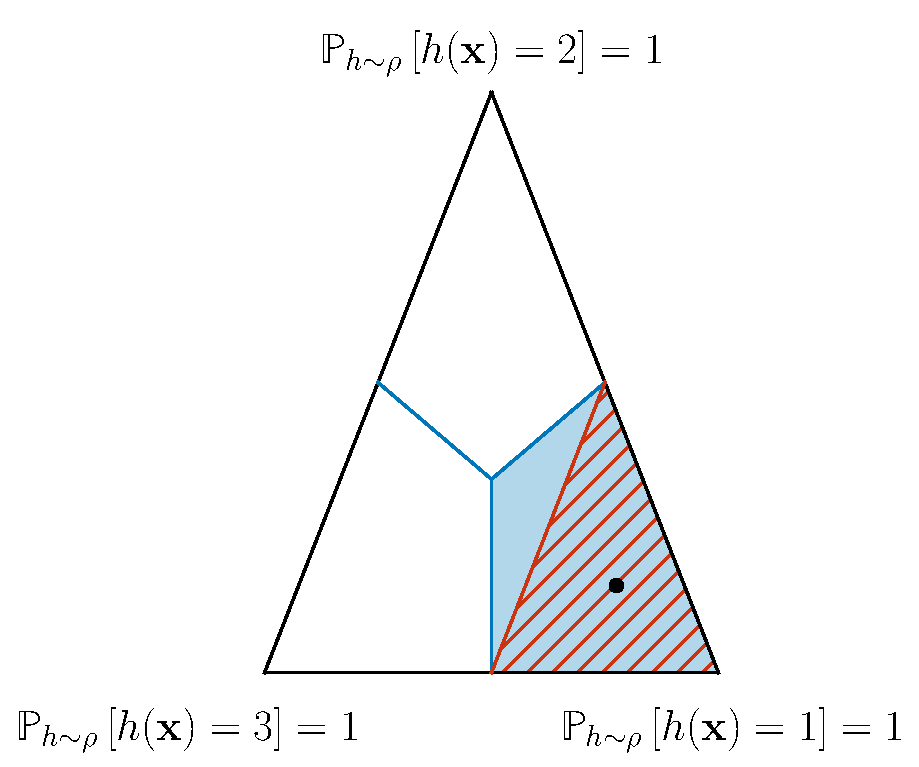
\includegraphics[width=0.5\textwidth]{chapter_2/figures/margin.pdf}
    \caption[Illustration of the Margin of the Majority Vote]{%
    Illustration of the majority vote's margin in the multi-class setting with 3 classes, \ie, $\Y=\{1, 2, 3\}$.
    The triangle represents the ternary plot of the three scores where each triangle's vertex is the three possible maximum scores with $\PP_{\h\sim\Q}\LB \h(\x)=i \RB=1$ for all $i\in\Y$.
    The black dot represents the prediction of an example $(\x, \y)\in\X\times\Y$ by the majority vote: the scores are $\PP_{\h\sim\Q}\LB \h(\x)=1 \RB=0.7$ and $\PP_{\h\sim\Q}\LB \h(\x)=2 \RB=\PP_{\h\sim\Q}\LB \h(\x)=3 \RB=0.15$.
    The blue area is where the majority vote predicts the label $\y$ for the input $\x$ and where the margin $\MaQ(\x,\y)$ is positive.
    Whereas the red area represents the predictions where $\PP_{\h\sim\Q}\LB \h(\x)=1 \RB\ge\frac{1}{2}$ (\ie, where the $\frac{1}{2}$-margin $\OmMaQ(\x,\y)$ is positive).
    }
    \label{chap:pac-bayes:fig:margin}
\end{figure}

The margin is positive if the score $\PP_{\h\sim\Q}\LB \h(\x)=\y \RB$ is higher than the score associated with the other labels $\y'\ne \y$ and is negative otherwise.
It captures if an example $(\x,\y)\sim\Dp$ is misclassified.
Indeed, thanks to the margin, the majority vote's risk $\Risk_{\Dp}(\MVQ)$ can be rewritten as follows:
\begin{align*}
\Risk_{\Dp}(\MVQ) &= \PP_{(\x,\y)\sim\Dp}\LB \PP_{\h\sim\Q}\LB \h(\x)=\y \RB \le \max_{\y'\in\Y, \y'\ne\y}\PP_{\h\sim\Q}\LB \h(\x)=\y' \RB \RB\\
&= \PP_{(\x,\y)\sim\Dp}\LB \MaQ(\x, \y) \le 0\RB.
\end{align*}

Hence, the risk is the probability that one of the scores is higher than the one of the correct label.
Unfortunately, deriving a learning algorithm to optimize the margin can be challenging since it is non-convex \wrt the posterior $\Q$ because of the $\max$.
To overcome this issue, \citet{LavioletteMorvantRalaivolaRoy2017} propose to consider a convex lower bound of the true margin called $\frac{1}{2}$-margin\footnote{We multiply the $\frac{1}{2}$-margin of \citet{LavioletteMorvantRalaivolaRoy2017} by two.}.

\begin{definition}[$\frac{1}{2}$-Margin of the Majority Vote]
For any hypothesis set $\H$, for any distribution $\Q$ on $\H$, the $\frac{1}{2}$-margin is defined as
\begin{align*}
    \OmMaQ(\x,\y) = 2\LB\PP_{\h\sim\Q}\LB \h(\x)=\y \RB - \frac{1}{2}\RB.
\end{align*}
\label{chap:pac-bayes:def:1/2-margin}
\end{definition}

When the score $\PP_{\h\sim\Q}\LB \h(\x)=\y \RB$ exceeds $\frac{1}{2}$, the majority vote surely classifies correctly the example $(\x, \y)\sim\Dp$.
Hence, the idea of this margin is to compute the difference between the score and $\frac{1}{2}$: when the margin is positive, the example is correctly classified.
We illustrate the difference between the two margins in \Cref{chap:pac-bayes:fig:margin}.
In binary classification, the $\frac{1}{2}$-margin boils down to $\OmMaQ(\x,\y) = \y\EE_{\h\sim\Q}\h(\x) = \EE_{\h\sim\Q}\Mah(\x,\y)$ (which is the margin introduced in \Cref{chap:intro:sec:loss-risk}).
From \Cref{chap:pac-bayes:def:1/2-margin}, we can deduce the following upper bound on the majority vote's risk, \ie, we have  
\begin{align*}
    \Risk_{\Dp}(\MVQ) &\le \PP_{(\x,\y)\sim\Dp}\LB \PP_{\h\sim\Q}\LB \h(\x)=\y \RB \le \frac{1}{2}\RB = \PP_{(\x,\y)\sim\Dp}\LB \OmMaQ(\x,\y) \le 0\RB.
\end{align*}

In general, the majority vote's risk $\Risk_{\Dp}(\MVQ)$ is not practical in learning algorithms because the gradient is zero (see \Cref{chap:intro:sec:loss-risk}).
Hence, in the next section, we recall different upper bounds on the majority vote's risk considered as surrogate losses.

\subsection{Upper Bounds on the Majority Vote's Risk}
\label{chap:pac-bayes:sec:surrogate}

We recall three surrogates on the majority vote's risk introduced in the literature, namely, the Gibbs Risk~\citep{LangfordShaweTaylor2002,McAllester2003}, the joint error~\citep{LacasseLavioletteMarchandGermainUsunier2006,GermainLacasseLavioletteMarchandRoy2015,MasegosaLorenzenIgelSeldin2020}, and the C-Bound~\citep{Breiman2001,LacasseLavioletteMarchandGermainUsunier2006,RoyLavioletteMarchand2011}.
We make use of these surrogate in \Cref{part:contrib-pac-bayes} to derive self-bounding learning algorithms.\footnote{A self-bounding algorithm, coined by \citet{Freund1998}, is a learning algorithm that comes with a generalization guarantee.}
More precisely, in \Cref{chap:mv-robustness}, we leverage the Gibbs risk for the adversarially robust setting and, in \Cref{chap:mv}, we learn majority vote classifiers through the C-Bound.

\subsubsection{The Gibbs Risk}

The first surrogate on the risk $\Risk_{\Dp}(\MVQ)$ introduced in the PAC-Bayesian literature is the {\it Gibbs risk} \citep{LangfordShaweTaylor2002,McAllester2003}.
This risk gives the average performance of individual voters in the majority vote. 
It is defined in the following way. 

\begin{definition}[Gibbs Risk]\label{chap:pac-bayes:def:gibbs} For any distribution $\Dp$ on $\X\times\Y$, for any hypothesis set $\H$, for any distribution $\Q$ on $\H$, the {\it Gibbs risk} is defined as
\begin{align*}
r_{\Dp}(\Q) \defeq \EE_{(\x,\y)\sim\Dp}   \EE_{\h\sim \Q} \indic\LB\h(\x) \ne \y\RB = \PP_{(\x,\y)\sim\Dp, \h\sim\Q}\LB \h(\x) \ne \y \RB.
\end{align*}
\end{definition}

Put into words, the Gibbs risk is the $\Q$-weighted average of the voters' risk.
Moreover, we can write the Gibbs Risk with respect to the $\frac{1}{2}$-margin. Indeed, we have 
\begin{align}
    r_{\Dp}(\Q) = \frac{1}{2}\LB 1-\EE_{(\x,\y)\sim\Dp}\OmMaQ(\x,\y)\RB.\label{chap:pac-bayes:eq:gibbs-margin}
\end{align}

\citet{LangfordShaweTaylor2002} show that the majority vote's risk is upper-bounded by twice the Gibbs risk.
The inequality is recalled in the following theorem. 

\begin{restatable}[Risk Upper Bound Based on the Gibbs Risk]{theorem}{theoremgibbs}\label{chap:pac-bayes:theorem:2gibbs} 
\looseness=-1
For any distribution $\Dp$ on $\X\times\Y$, for any hypothesis set $\H$, for any distribution $\Q$ on $\H$, we have
\begin{align}
\Risk_{\Dp}(\MVQ) \leq 2\, r_{\Dp}(\Q).
\label{chap:pac-bayes:eq:2gibbs}
\end{align}
\end{restatable}
\begin{noaddcontents}\begin{proof}
Deferred to~\Cref{ap:pac-bayes:sec:proof-2gibbs}.
\end{proof}\end{noaddcontents}

However, in ensemble methods where one wants to combine voters efficiently, the Gibbs risk appears to be an imprecise surrogate since the combination of voters might compensate for individual errors.
Hence, other surrogates need to be taken into account.

\subsubsection{Joint Error}

The joint error, introduced by \citet{LacasseLavioletteMarchandGermainUsunier2006}, takes better the voters' correlation into account; this quantity is defined in the following way.

\begin{definition}[Joint Error]\label{chap:pac-bayes:def:joint} For any distribution $\Dp$ on $\X\times\Y$, for any hypothesis set $\H$, for any distribution $\Q$ on $\H$, the {\it joint error} is defined as
\begin{align*}
    e_{\Dp}(\Q) &\defeq \EE_{(\x,\y)\sim\Dp} \EE_{\h\sim\Q}\EE_{\h'\sim\Q}
     \indic\LB\h(\x) \ne \y\big]\indic\big[\h'(\x) \ne \y\RB\\
    &= \PP_{(\x,\y)\sim\Dp, \h\sim\Q, \h'\sim\Q}\LB\h(\x) \ne \y, \h'(\x) \ne \y\RB.
\end{align*}
\end{definition}

Similarly to \Cref{chap:pac-bayes:eq:gibbs-margin} for the Gibbs risk, we can reinterpret this surrogate with the $\frac{1}{2}$-margin.
Indeed, from \citet{GermainLacasseLavioletteMarchandRoy2015}, we have 
\begin{align}
    e_{\Dp}(\Q) &= \EE_{(\x,\y)\sim\Dp}\LP \PP_{\h\sim\Q}\LB \h(\x)\ne\y\RB\RP^2\nonumber\\
    &= \EE_{(\x,\y)\sim\Dp}\LP\frac{1}{2}\LB1-\OmMaQ(\x,\y)\RB\RP^2\nonumber\\
    &= \frac{1}{4}\LP 1-2\EE_{\h\sim\Q}\OmMaQ(\x,\y) + \EE_{\h\sim\Q}\OmMaQ(\x,\y)^2\RP.\label{chap:pac-bayes:eq:joint-margin} 
\end{align}

Recently, \citet{MasegosaLorenzenIgelSeldin2020} proposed to deal directly with the joint error to bound the majority vote's risk; Their bound is presented in the following theorem.

\begin{restatable}[Risk Upper Bound Based on the Joint Error]{theorem}{theoremjoint}\label{chap:pac-bayes:theorem:4joint}
\looseness=-1
For any distribution $\Dp$ on $\X\times\Y$, for any hypothesis set $\H$, for any distribution $\Q$ on $\H$, we have
\begin{align}
    \Risk_{\Dp}(\MVQ) \le 4e_{\Dp}(\Q). 
    \label{chap:pac-bayes:eq:4joint}
\end{align}
\end{restatable}
\begin{noaddcontents}\begin{proof}
Deferred to~\Cref{ap:pac-bayes:sec:proof-4joint}.
\end{proof}\end{noaddcontents}

\looseness=-1
This inequality captures the fact that the voters need to be sufficiently diverse and commit errors on different points.
However, when the joint error $e_{\Dp}(\Q)$ exceeds~$\frac14$, the bound exceeds $1$ and is uninformative.
In some cases, these two upper bounds appear to be less tight than another one: the C-Bound~\citep{Breiman2001,LacasseLavioletteMarchandGermainUsunier2006}. 

\subsubsection{The C-Bound}

The C-Bound\footnote{The term ``C-Bound'' was introduced in the PAC-Bayesian literature by \citep{LacasseLavioletteMarchandGermainUsunier2006}.} \citep{Breiman2001,LacasseLavioletteMarchandGermainUsunier2006} is another surrogate (and upper bound) of the majority vote's risk.
It is derived from the \textsc{Chebyshev}-\textsc{Cantelli} Inequality (see \Cref{ap:tools:theorem:cantelli}).
It depends on the {\it Gibbs risk}, the {\it joint error}, and the {\it disagreement}.
This latter is defined in the following way.

\begin{definition}[Disagreement]\label{chap:pac-bayes:def:disagreement} For any distribution $\Dp$ on $\X\times\Y$, for any hypothesis set $\H$, for any distribution $\Q$ on $\H$, the {\it disagreement} is defined as
\begin{align*}
    d_{\Dp}(\Q) &\defeq 2\EE_{(\x,\y)\sim\Dp}\EE_{\h\sim\Q}\EE_{\h'\sim\Q}\indic\LB \h(\x)\ne \y\RB\indic\LB \h'(\x)=\y\RB\\
    &= 2\PP_{(\x,\y)\sim\Dp, \h\sim\Q, \h'\sim\Q}\LB \h(\x)\ne \y, \h'(\x)=\y\RB.
\end{align*}
\end{definition}

The higher the disagreement, the more the voters do not perform the same prediction for a given $(\x,\y)\sim\Dp$.
Similarly to the Gibbs risk and the joint error, we can express the disagreement with the margin.
Indeed, we have
\begin{align}
    d_{\Dp}(\Q) = \frac{1}{2}\LB 1 - \EE_{(\x,\y)\sim\Dp}\OmMaQ(\x,\y)^2\RB.\label{chap:pac-bayes:eq:disagreement-margin}
\end{align}

Interestingly, by developing \Cref{chap:pac-bayes:eq:joint-margin}, we can relate the Gibbs risk and the joint error to the disagreement with
\begin{align}
    d_{\Dp}(\Q) = 2\LB r_{\Dp}(\Q) - e_{\Dp}(\Q)\RB.\label{chap:pac-bayes:eq:disagreement-risk-joint}
\end{align}
This inequality tells us two facts: {\it (i)} the lower the Gibbs risk, the lower the disagreement, and {\it (ii)} the disagreement increases as the joint error decreases.
The expression of the disagreement in binary classification can be simplified (with voters $\h:\X\to \{-1, +1\}$).
Indeed, given an example $(\x, \y)\sim\Dp$ with $\y\in\{-1, +1\}$, we have
\begin{align*}
    \PP_{\h\sim\Q, \h'\sim\Q}\LB \h(\x)\ne\h'(\x)\RB &= \PP_{\h\sim\Q, \h'\sim\Q}\LB \h(\x)=\y, \h'(\x)\ne\y \RB + \PP_{\h\sim\Q, \h'\sim\Q}\LB \h(\x)\ne\y, \h'(\x){=}\y \RB\\
    &= 2\PP_{\h\sim\Q, \h'\sim\Q}\LB \h(\x)\ne \y, \h'(\x)=\y\RB,
\end{align*}
which gives $d_{\Dp}(\Q)=\PP_{(\x,\y)\sim\Dp, \h\sim\Q, \h'\sim\Q}\LB \h(\x)\ne\h'(\x)\RB$.

Thanks to this quantity, we are now able to recall the C-Bound.
Note that it was first introduced by \citet{LacasseLavioletteMarchandGermainUsunier2006} for the PAC-Bayesian majority vote in binary classification.
The generalization to the multi-class setting has been introduced by \citet[Theorem~2 and Corollary~1]{LavioletteMorvantRalaivolaRoy2017}; we recall the C-Bound in the following theorem.

\begin{restatable}[The C-Bound]{theorem}{theoremgeneralcbound}\label{chap:pac-bayes:theorem:cbound}
For any distribution $\Dp$ on $\X\times\Y$, for any hypothesis set $\H$, for any distribution $\Q$ on $\H$, if 
\begin{align*}
\EE_{(\x,\y)\sim\Dp}\OmMaQ(\x,\y) > 0 \iff r_{\Dp}(\Q)<\tfrac{1}{2}\iff2e_{\Dp}(\Q)+d_{\Dp}(\Q)<1,
\end{align*}
we have
\begin{align}
\Risk_{\Dp}(\MVQ) &\le 1-\frac{\LP\EE_{(\x,\y)\sim\Dp}\LB \OmMaQ(\x,\y)\RB\RP^2}{\EE_{(\x,\y)\sim\Dp}\LP \OmMaQ(\x,\y)\RP^2}\label{chap:pac-bayes:eq:multi-class-cbound}\\
&= 1-\frac{\LP1-2r_{\Dp}(\Q)\RP^2}{1-2d_{\Dp}(\Q)}\label{chap:pac-bayes:eq:cbound-r-d}\\
    &= 1-\frac{\big(1-\LB2e_{\Dp}(\Q)+d_{\Dp}(\Q)\RB\big)^2}{1-2d_{\Dp}(\Q)}\label{chap:pac-bayes:eq:cbound-e-d} \\ 
    &= \CBound_{\Dp}(\Q).\nonumber
\end{align}
\end{restatable}
\begin{noaddcontents}\begin{proof}
Deferred to~\Cref{ap:pac-bayes:sec:proof-cbound}.
\end{proof}\end{noaddcontents}

This surrogate is expressed as a trade-off between the first and the second statistical moment of the $\frac{1}{2}$-margin $\OmMaQ(\x,\y)$ (\Cref{chap:pac-bayes:eq:multi-class-cbound}).
Based on \Cref{chap:pac-bayes:eq:gibbs-margin,chap:pac-bayes:eq:disagreement-margin}, the trade-off can be expressed through the the disagreement and the Gibbs risk (see \Cref{chap:pac-bayes:eq:cbound-r-d}).
Moreover, from \Cref{chap:pac-bayes:eq:disagreement-risk-joint}, we can also see the C-Bound as a trade-off between the joint error and the disagreement in \Cref{chap:pac-bayes:eq:cbound-e-d}.\\

The three surrogates of \Cref{chap:pac-bayes:theorem:2gibbs,chap:pac-bayes:theorem:4joint,chap:pac-bayes:theorem:cbound} can be easily compared.
For instance, when $r_{\Dp}(\Q) \leq d_{\Dp}(\Q)$, the C-Bound $\CBound_{\Dp}(\Q)$ (\Cref{chap:pac-bayes:eq:multi-class-cbound}) is tighter than $2r_{\Dp}(\Q)$ (\Cref{chap:pac-bayes:eq:2gibbs}) and $4e_{\Dp}(\Q)$ (\Cref{chap:pac-bayes:eq:4joint}).
Hence, when the disagreement increases, the C-Bound appears to be a good trade-off between the Gibbs risk and the disagreement.
More precisely, the main interest of the C-bound compared to \Cref{chap:pac-bayes:eq:4joint} is that when $e_{\Dp}(\Q)$ is close to $\tfrac{1}{4}$, the C-Bound can be close to $0$ depending on the value of the disagreement $d_{\Dp}(\Q)$: the C-bound is then more precise.
Moreover, it is important to notice that the C-Bound is tighter than $4e_{\Dp}(\Q)$ for all cases.
We summarize the relationships between the different surrogates in the next theorem and illustrate it in \Cref{chap:pac-bayes:fig:cbound}; this relation is notably given by \citet{GermainLacasseLavioletteMarchandRoy2015} and \citet{MasegosaLorenzenIgelSeldin2020}.

\begin{restatable}[Relationship between \Cref{chap:pac-bayes:theorem:2gibbs,chap:pac-bayes:theorem:4joint,chap:pac-bayes:theorem:cbound}]{theorem}{theoremrelationship}\label{chap:pac-bayes:theorem:relationship}
 For any distribution $\D$ on $\X\times\Y$, for any voters set $\H$, for any distribution $\Q$ on $\H$, if $r_{\Dp}(\Q) < \tfrac{1}{2}$ (\ie, $\EE_{(\x,\y)\sim\Dp}\OmMaQ(\x,\y) > 0$), we have
\begin{center}
\begin{enumerate}[\it (i)]
    \item $\Risk_{\Dp}(\MVQ) \le C_{\Dp}(\Q) \le 4e_{\Dp}(\Q) \le 2r_{\Dp}(\Q)$, if  $r_{\Dp}(\Q) \le d_{\Dp}(\Q)$,
    \item $\Risk_{\Dp}(\MVQ) \le 2r_{\Dp}(\Q) \le C_{\Dp}(\Q) \le 4e_{\Dp}(\Q)$,\quad otherwise.
\end{enumerate}
\end{center}
\end{restatable}
\begin{noaddcontents}\begin{proof}
Deferred to~\Cref{ap:pac-bayes:sec:proof-relationship}.
\end{proof}\end{noaddcontents}

\begin{figure}
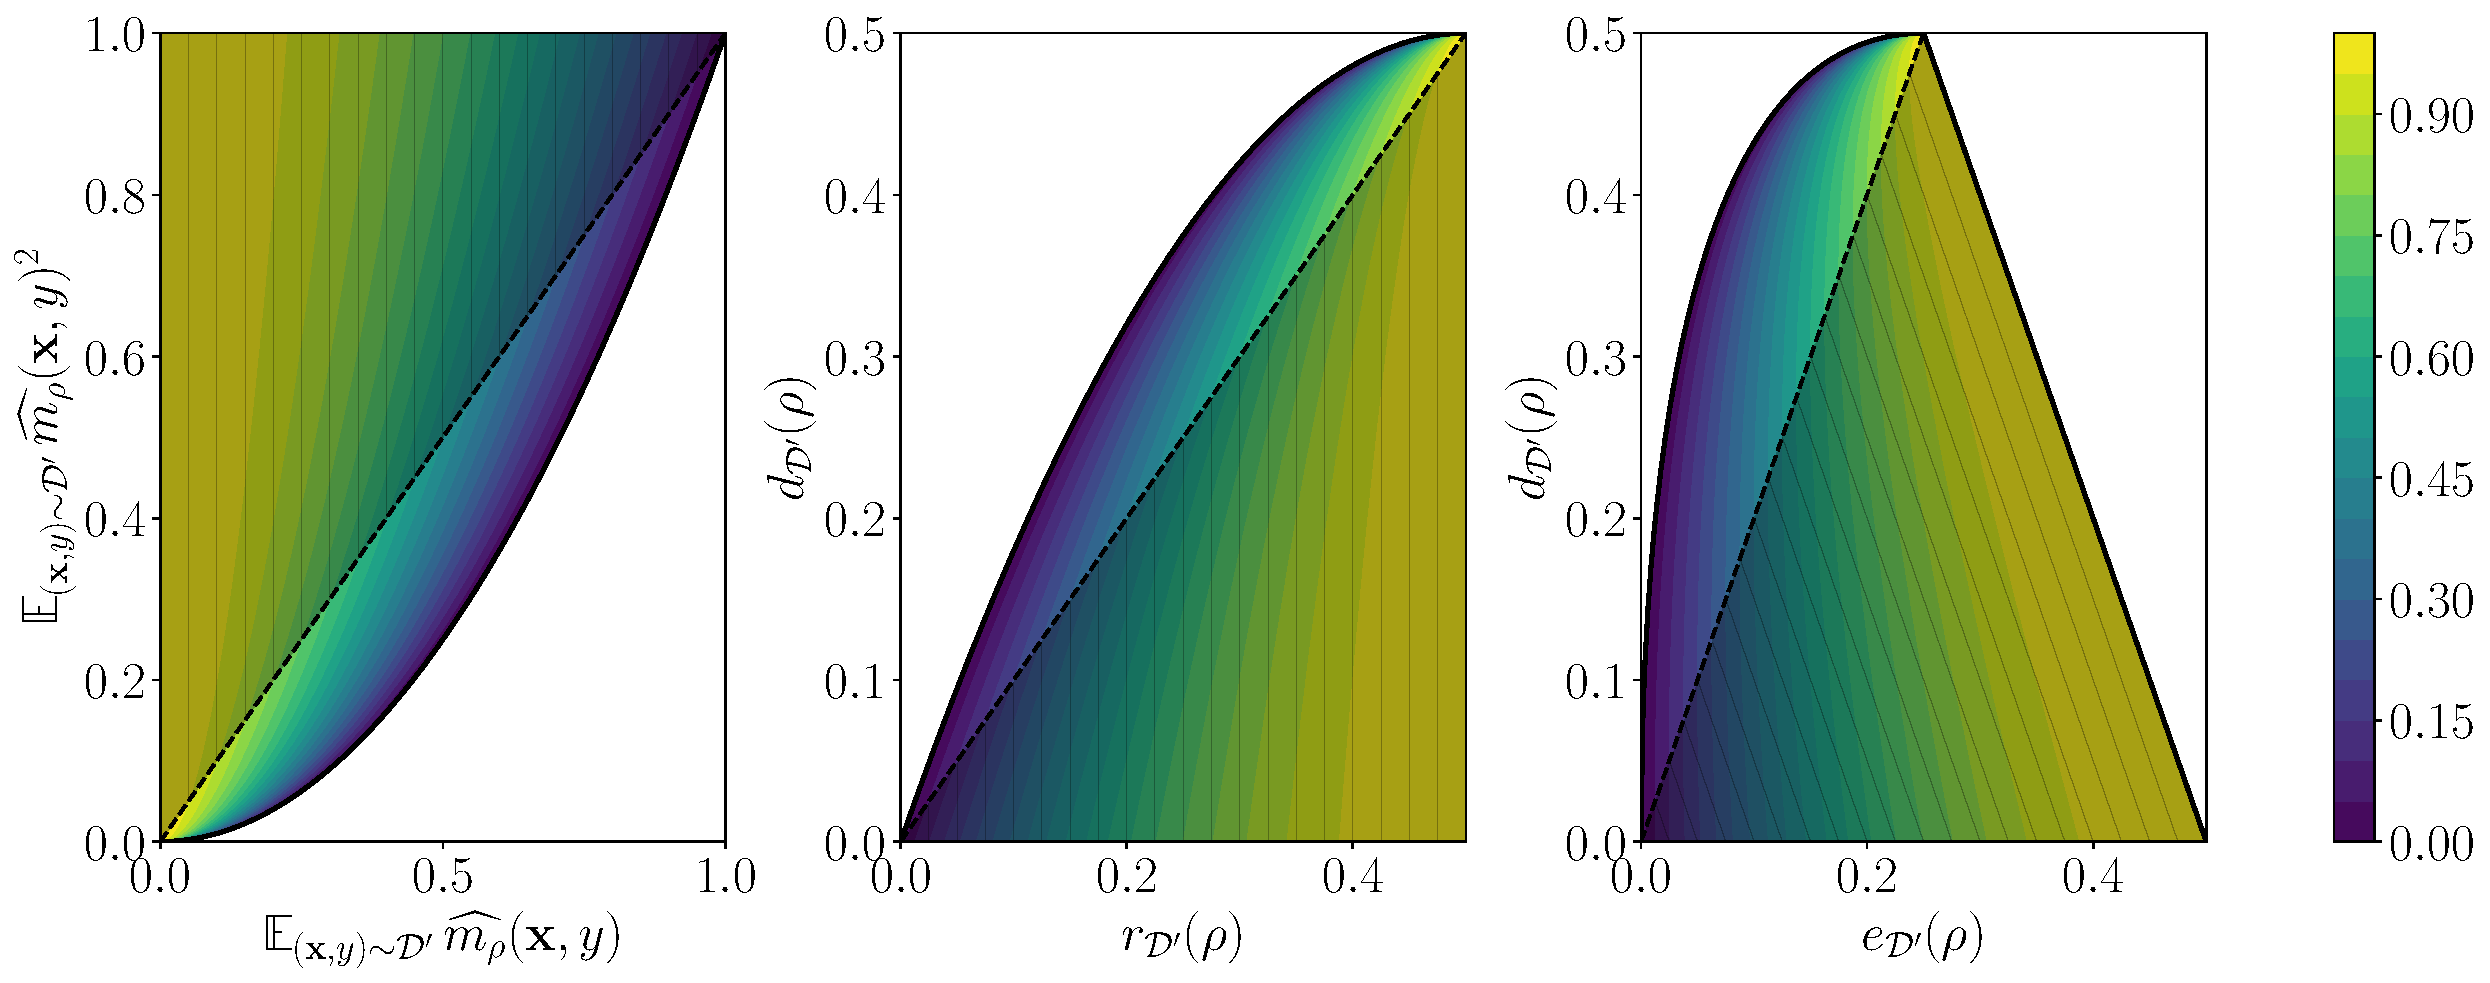
\includegraphics[width=1.0\textwidth]{chapter_2/figures/cbound.pdf}
\caption[Plots that Summarize the Relationship Between the Surrogates]{
Plots (from left to right) of the different C-Bounds in \Cref{chap:pac-bayes:eq:multi-class-cbound,chap:pac-bayes:eq:cbound-r-d,chap:pac-bayes:eq:cbound-e-d}.
For each plot, the darker area represents the cases where $2r_{\Dp}(\Q)$ is tighter than the C-Bound $\CBound_{\Dp}(\Q)$.
The  dashed line represents the cases where $4e_{\Dp}(\Q)$ matches the C-Bound $\CBound_{\Dp}(\Q)$.
}
\label{chap:pac-bayes:fig:cbound}
\end{figure}



Since the distribution $\D$ is unknown, the true risk of the majority vote $\Risk_{\D}(\MVQ)$ is not computable.
Hence, one can minimize the empirical risk of the majority vote $\Risk_{\dS}(\MVQ)$ through the Empirical Risk Minimization approach (see \Cref{chap:intro:algo:erm}).
However, this minimization does not necessarily lead to a low true risk $\Risk_{\D}(\MVQ)$ since overfitting can occur (see \Cref{chap:intro:sec:selection}).
To tackle this issue, one solution is to deal with the minimization of a generalization bound to get a self-bounding algorithm~\citep{Freund1998}, \ie, the  minimization of the risk with generalization guarantees.
We will see in the next section PAC-Bayesian generalization bounds that further allow us to upper-bound the true risk $\Risk_{\D}(\MVQ)$ in \Cref{part:contrib-pac-bayes}.

\section{PAC-Bayesian Bounds}
\label{chap:pac-bayes:sec:pac-bayes}

The PAC-Bayesian theory\footnote{See \citep{Guedj2019,Alquier2021} for recent on the PAC-Bayesian theory.}, introduced by \citet{ShaweTaylorWilliamson1997} and \citet{McAllester1999}, aims to provide PAC generalization bounds for Bayesian-like algorithms.
Such Bayesian algorithms assume a probability distribution defined {\it apriori} on the hypothesis set $\H$, and thanks to Bayes' theorem, obtain an {\it a posteriori} probability distribution on $\H$ thanks to the learning sample; see \citet{Bishop2007} for more details on this Bayesian inference procedure.
Contrary to the classical Bayesian inference where the {\it posterior} distribution is proportional to the product of the {\it prior} distribution and the likelihood of the data, in PAC-Bayesian theory, an arbitrary {\it prior} distribution can be considered.
Actually, the term ``Bayesian'' in the PAC-Bayesian theory comes from the fact that we usually upper-bound the {\it expected} generalization gap $\LN \EE_{\h\sim\AQ}\RiskLoss_{\D}(\h)-\EE_{\h\sim\AQ}\RiskLoss_{\dS}(\h)\RN$ where $\h\in\H$ is sampled from a data-dependent distribution $\AQ$ called {\it posterior}.
This theory has been extended to various settings such as transductive learning~\citep{DerbekoElYanivMeir2004, BeginGermainLavioletteRoy2014}, regression~\citep{GermainBachLacosteLacosteJulien2016, ShalaevaEsfahaniGermainPetreczky2020}, structured prediction~\citep{LavioletteMorvantRalaivolaRoy2017}, domain adaptation~\citep{GermainHabrardLavioletteMorvant2020}, or randomized learning~\citep{London2017}.\\

In order to define a PAC-Bayesian bound more formally, we denote by $\AQ$ (or $\Q$) the {\it posterior} distribution on $\H$ and $\P$ the {\it prior} distribution.
Each probability distribution $\Q$ is defined through its probability density function $\h \mapsto \Q(\h)$ with respect to a reference measure\footnote{For instance, if $\H=\Rbb^{d}$, then the reference measure is the Lebesgue one.} on $\H$; we denote by $\M(\H)$ the set of probability density function on $\H$.
Hence, the distribution $\AQ\in\M(\H)$ is the Radon–Nikodym derivative of a probability measure \wrt the reference measure.
We also denote by $\M^{*}(\H)\subseteq\M(\H)$ the set of strictly positive probability densities on $\H$.
Moreover, for convenience, we assume that the support of the posterior $\AQ$ is in the support of $\P$, \ie, if $\P(\h)=0$ then $\AQ(\h)=0$ (the absolute continuity); hence $\P\in\M^{*}(\H)$.\\

\looseness=-1
With the setting in place, we can now define the general form of a PAC-Bayesian bound in the following.

\begin{restatable}[PAC-Bayesian Generalization Bound]{definition}{definitionpacbayes}\label{chap:pac-bayes:def:pac-bayes}
Let $\loss: \H \times(\X{\times}\Y)\rightarrow [0,1]$ be a loss function and $\phi: [0,1]^2{\to}\Rbb$ a generalization gap. 
A PAC-Bayesian bound is defined such that if for any distribution $\D$ on $\X\times\Y$, for any hypothesis set $\H$, for any prior distribution $\P\in\M^{*}(\H)$ on $\H$, there exists a function $\Phi: \M(\H){\times}\M^{*}(\H){\times}(0,1]{\to} \Rbb$, such that for any $\delta\in(0, 1]$ we have 
\begin{align*}
    \PP_{\S\sim\D^\m}\LB \phi({\textstyle\EE_{\h\sim\AQ}\RiskLoss_{\D}(\h)}, {\textstyle\EE_{\h\sim\AQ}\RiskLoss_{\dS}(\h)}) \le \Phi\big(\AQ, \P, \delta\big) \RB \ge 1-\delta,
\end{align*}
where \eg $\phi({\textstyle\EE_{\h\sim\AQ}\RiskLoss_{\D}(\h)}, {\textstyle\EE_{\h\sim\AQ}\RiskLoss_{\dS}(\h)}) = \LN\EE_{\h\sim\AQ}\RiskLoss_{\D}(\h)-\EE_{\h\sim\AQ}\RiskLoss_{\dS}(\h)\RN$.
\end{restatable}

\Cref{chap:pac-bayes:def:pac-bayes} is a general definition in the sense that the expected generalization gap  $\LN\EE_{\h\sim\AQ}\RiskLoss_{\D}(\h)-\EE_{\h\sim\AQ}\RiskLoss_{\dS}(\h)\RN$ is not the only usable deviation between the true risk $\EE_{\h\sim\AQ}\RiskLoss_{\D}(\h)$ and the empirical risk $\EE_{\h\sim\AQ}\RiskLoss_{\dS}(\h)$.
For example, one can consider the one-sided difference $\EE_{\h\sim\AQ}\RiskLoss_{\D}(\h)-\EE_{\h\sim\AQ}\RiskLoss_{\dS}(\h)$ or the squared difference $\LB\EE_{\h\sim\AQ}\RiskLoss_{\D}(\h)-\EE_{\h\sim\AQ}\RiskLoss_{\dS}(\h)\RB^2$.
As we will see in this chapter, several gaps $\phi()$ have been considered in the literature.
These gaps are upper-bounded with probability at least $1{-}\delta$ with a function $\Phi()$ that depends on $\delta$ and two probability distributions on $\H$.
Usually, the lower the parameter $\delta\in(0, 1]$, the higher the upper bound $\Phi()$, \ie, the function $\Phi()$ is decreasing \wrt $\delta$.
Moreover, this upper bound $\Phi()$ depends on a data-dependent {\it posterior} distribution $\AQ\in\M(\H)$ and a {\it prior} distribution $\P\in\M^{*}(\H)$.
The prior distribution is data-free and can incorporate prior knowledge, \eg, coming from an expert knowledge or an additional learning sample~\citep{ParradoHernandezAmbroladzeShaweTaylorSun2012,DziugaiteHsuGharbiehArpinoRoy2021}.
In the rest of the section, we present different instantiations of \Cref{chap:pac-bayes:def:pac-bayes}, making an overview of the PAC-Bayesian bounds in the literature.

\subsection{General PAC-Bayesian Bound of \citet{GermainLacasseLavioletteMarchand2009}}

There are different kinds of bounds in the PAC-Bayesian literature~\citep[\eg,][]{Seeger2002, McAllester2003, Catoni2007}. 
Several existing bounds can be proved from a general theorem by \citet{GermainLacasseLavioletteMarchand2009}; it is recalled in the following theorem.

\begin{restatable}[General PAC-Bayesian Bound of \citet{GermainLacasseLavioletteMarchand2009}]{theorem}{generalgermain}\label{chap:pac-bayes:theorem:general-germain}
For any distribution $\D$ on $\X{\times}\Y$, for any hypothesis set $\H$, for any distribution $\P\in\M^{*}(\H)$ on $\H$, for any measurable function $\varphi: \H\times(\X\times\Y)^\m\to \Rbb$, we have
\begin{align*}
    \PP_{\S\sim\D^\m}\LB \forall\Q\in\M(\H),\  \EE_{\h\sim\Q}\varphi(\h, \S) \le \KL(\Q\|\P) + \ln\LP\frac{1}{\delta}\EE_{\S'\sim\D^\m}\EE_{\h'\sim\P}e^{\varphi(\h', \S')}\RP \RB\ge1{-}\delta,
\end{align*}
where $\displaystyle\KL(\Q\|\P){=}\EE_{\h\sim\Q}\ln\!\frac{\Q(\h)}{\P(\h)}$ is the Kullback-Leibler (KL) divergence between the distributions $\Q$ and $\P$.
\end{restatable}
\begin{noaddcontents}\begin{proof}
Deferred to~\Cref{ap:pac-bayes:sec:proof-general-germain}.
\end{proof}\end{noaddcontents}

Note that this bound holds for all posterior distributions $\Q\in\M(\H)$, which includes notably the prior distribution $\P$, or any data-dependent posterior $\AQ$.
Furthermore, this bound is penalized by the KL divergence\footnote{The principal properties of the KL divergence are given in \Cref{ap:pac-bayes:sec:kl}} between $\Q$ and $\P$. 
The closer the posterior $\Q$ is to the prior $\P$, the smaller the divergence and the bound.
Moreover, the bound holds for a function $\varphi: \H\times(\X\times\Y)^\m\to \Rbb$ that further captures a deviation between the true risk $\RiskLoss_{\D}(\h)$ and the empirical risk $\RiskLoss_{\dS}(\h)$.
For example, with $\varphi(\h,\S)=\m\phi(\RiskLoss_{\D}(\h),\RiskLoss_{\dS}(\h))$ where $\phi()$ is convex, we are able to retrieve \Cref{chap:pac-bayes:def:pac-bayes}. 
By setting this function $\phi()$ accordingly, one can retrieve some classical bounds that have been previously introduced in the literature~\citep{McAllester2003,Seeger2002,Catoni2007} as we show further.

\subsubsection{\citeauthor{McAllester2003}-like bound}

First of all, we can retrieve \Cref{chap:intro:theorem:maurer} presented in \Cref{chap:intro} which is a tighter version of the bound derived by \citet[Theorem~1]{McAllester2003}.
Indeed, by setting $\varphi(\h,\S)=2\m\LB\RiskLoss_{\D}(\h)-\RiskLoss_{\dS}(\h)\RB^2$ in \Cref{chap:pac-bayes:theorem:general-germain}, one can deduce the following result.

\begin{restatable}[PAC-Bayesian Bound of \citet{McAllester2003}]{theorem}{mcallester}\label{chap:pac-bayes:theorem:mcallester}
For any distribution $\D$ on $\X\times\Y$, for any hypothesis $\H$, for any prior $\P\in\M^{*}(\H)$, for any loss $\loss: \H{\times}(\X\times\Y)^\m \to [0, 1]$, for any $\delta\in(0, 1]$, we have
\begin{align}
    \PP_{\S\sim\D^\m}\LB \forall\Q\in\M(\H), \LN\EE_{\h\sim\Q}\RiskLoss_{\D}(\h){-}\EE_{\h\sim\Q}\RiskLoss_{\dS}(\h)\RN \le \sqrt{\frac{1}{2\m}\!\LB\KL(\Q\|\P){+}\ln\tfrac{2\sqrt{\m}}{\delta}\RB}\RB \ge 1{-}\delta.\label{chap:pac-bayes:eq:mcallester}
\end{align}
\end{restatable}
\begin{noaddcontents}\begin{proof}
Deferred to~\Cref{ap:pac-bayes:sec:proof-mcallester}.
\end{proof}\end{noaddcontents}

According to \Cref{chap:pac-bayes:theorem:mcallester}, the gap $|\EE_{\h\sim\Q}\RiskLoss_{\D}(\h){-}\EE_{\h\sim\Q}\RiskLoss_{\dS}(\h)|$ tends to zero when the number of examples increase.
Hence, the more examples we have, the closer the expected empirical risk $\EE_{\h\sim\Q}\RiskLoss_{\dS}(\h)$  is from expected true empirical risk $\EE_{\h\sim\Q}\RiskLoss_{\D}(\h)$ for all $\Q\in\M(\H)$.
Actually, bounding this gap gives an upper bound on the expected true risk.
Indeed, with probability at least $1{-}\delta$ over the random choice of $\S{\sim}\D^\m$, we have 
\begin{align}
    \forall\Q\in\M(\H),\quad &\EE_{\h\sim\Q}\RiskLoss_{\D}(\h) \le \EE_{\h\sim\Q}\RiskLoss_{\dS}(\h) + \sqrt{\frac{1}{2\m}\!\LB\KL(\Q\|\P){+}\ln\tfrac{2\sqrt{\m}}{\delta}\RB}\label{chap:pac-bayes:eq:mcallester-1}\\
    \text{and}\quad &\EE_{\h\sim\Q}\RiskLoss_{\D}(\h) \ge \EE_{\h\sim\Q}\RiskLoss_{\dS}(\h) - \sqrt{\frac{1}{2\m}\!\LB\KL(\Q\|\P){+}\ln\tfrac{2\sqrt{\m}}{\delta}\RB}\label{chap:pac-bayes:eq:mcallester-2}
\end{align}

Put into words, the expected true risk $\EE_{\h\sim\Q}\RiskLoss_{\D}(\h)$ can be lower and upper bounded by the expected empirical risk $\EE_{\h\sim\Q}\RiskLoss_{\dS}(\h)$ and the bound $\sqrt{\frac{1}{2\m}[\KL(\Q\|\P){+}\ln\frac{2\sqrt{\m}}{\delta}]}$.
When our objective is to obtain a low expected true risk $\EE_{\h\sim\Q}\RiskLoss_{\D}(\h)$, one can obtain a distribution $\Q\in\M(\H)$ minimizing the bound with the minimization problem 
\begin{align*}
    \min_{\Q\in\M(\H)} \LC \EE_{\h\sim\Q}\RiskLoss_{\dS}(\h) + \sqrt{\frac{1}{2\m}\!\LB\KL(\Q\|\P){+}\ln\tfrac{2\sqrt{\m}}{\delta}\RB} \RC.
\end{align*}

Since the bound holds for all $\Q\in\M(\H)$ (with high probability), it also holds for the optimal solution.
The contributions in \Cref{part:contrib-pac-bayes} rely on such a minimization problem to obtain models with a certified expected test risk.
Nevertheless, as we will see further, the bound of \Cref{chap:pac-bayes:theorem:mcallester} is not the tightest.

\subsubsection{\citeauthor{Catoni2007}-like bound}
\label{chap:pac-bayes:subsubsection:catoni-germain}

\citet[Theorem 1.2.1]{Catoni2007} proposed a bound that can be tighter than the one of \Cref{chap:pac-bayes:theorem:mcallester} by considering a parameter $\cat>0$.
His proposed bound can be retrieved from \Cref{chap:pac-bayes:theorem:general-germain} by defining $\varphi(\h,\S) = \m\phi(\RiskLoss_{\D}(\h), \RiskLoss_{\dS}(\h))$ where the deviation is $\phi(\RiskLoss_{\D}(\h), \RiskLoss_{\dS}(\h))=-\ln\!\LP 1{-}\LP1{-}e^{-\cat}\RP\RiskLoss_{\D}(\h)\RP-\cat\RiskLoss_{\dS}(\h)$. 
We state the bound in the following theorem.

\begin{restatable}[PAC-Bayesian Bound of \citet{Catoni2007}]{theorem}{catoni}\label{chap:pac-bayes:theorem:catoni}
For any distribution $\D$ on $\X\times\Y$, for any hypothesis $\H$, for any prior $\P\in\M^{*}(\H)$, for any loss $\loss: \H{\times}(\X\times\Y)^\m \to [0, 1]$, for any $\cat>0$, for any $\delta\in(0, 1]$, we have
\begin{align}
    \PP_{\S\sim\D^\m}\Bigg[ \forall\Q\in\M(\H), 
    -\ln\!\LP 1{-}\LB1{-}e^{{-}\cat}\RB\EE_{\h\sim\Q}\RiskLoss_{\D}(\h)\RP&-\cat\EE_{\h\sim\Q}\RiskLoss_{\dS}(\h)\nonumber\\
    &\hspace{-2cm}\le \frac{1}{\m}\LB\KL(\Q\|\P){+}\ln\frac{1}{\delta}\RB\Bigg] \ge 1-\delta.\label{chap:pac-bayes:eq:catoni}
\end{align}
\end{restatable}
\begin{noaddcontents}\begin{proof}
Deferred to~\Cref{ap:pac-bayes:sec:proof-catoni}.
\end{proof}\end{noaddcontents}

The result is difficult to interpret because of the gap $-\ln\!\LP 1{-}\LB1{-}e^{{-}\cat}\RB\EE_{\h\sim\Q}\RiskLoss_{\D}(\h)\RP-\cat\EE_{\h\sim\Q}\RiskLoss_{\dS}(\h)$ is not easy to analyze.
However, rewriting it as an upper bound of the expected true risk $\EE_{\h\sim\Q}\RiskLoss_{\D}(\h)$ makes its interpretation easier.
Indeed, with probability at least $1-\delta$ over the random choice of $\S\sim\D^\m$, we have
\begin{align*}
\forall\Q\in\M(\H),\ \EE_{\h\sim\Q}\RiskLoss_{\D}(\h) \le \frac{1}{1{-}e^{{-}\cat}}\Bigg[1{-}\exp\Bigg(\!{-}\cat\EE_{\h\sim\Q}\RiskLoss_{\dS}(\h){-}\frac{1}{\m}\LB\KL(\Q\|\P){+}\ln\frac{1}{\delta}\RB\Bigg)\Bigg].
\end{align*}

Put into words, the expected true risk $\EE_{\h\sim\Q}\RiskLoss_{\D}(\h)$ is upper-bounded by a trade-off, controlled by the parameter $\cat$, between the expected empirical risk $\EE_{\h\sim\Q}\RiskLoss_{\dS}(\h)$ and the term $\frac{1}{\m}\LB \KL(\Q\|\P){+}\ln\frac{1}{\delta} \RB$.
This is in contrast with \Cref{chap:pac-bayes:eq:mcallester,chap:pac-bayes:eq:mcallester-1,chap:pac-bayes:eq:mcallester-2} since this bound depends on a parameter $\cat>0$, which allows one to tune the tightness of the bound.

In practice, it is hard to set the parameter $\cat$ since the bound holds with high probability on $\S\sim\D^\m$ for all parameters $\cat>0$. 
Hence, it is not possible to condition $\cat$ on $\S\sim\D^\m$. 
To tackle this issue, one usually applies a union bound to get a bound holding for any $\cat$ belonging to a countable set.
Hopefully, as shown further, one can derive a bound that avoids this parameter and is potentially tighter.

\subsubsection{\citeauthor{Seeger2002}-like bound}
\label{chap:pac-bayes:subsubsection:seeger-germain}

One of the tightest PAC-Bayesian bound (that avoids the parameter $\cat$) is the one proven by \citet{Seeger2002}.
This bound depends on the KL divergence between two Bernoulli distributions.
This function is defined in the following way.

\begin{definition}[KL Divergence Between Two Bernoulli Distributions]
For any distribution $q\in[0,1]$ and $p\in[0,1]$, the small kl is defined as
\begin{align*}
\kl(q\|p)\defeq \KL(\Bernoulli(q)\|\Bernoulli(p)) = q\ln\frac{q}{p}+(1{-}q)\ln\frac{1{-}q}{1{-}p},
\end{align*}
where $\Bernoulli(q)$ and $\Bernoulli(p)$ are two Bernoulli distributions with bias $q$ and $p$. 
\end{definition}

The first PAC-Bayesian theorem based on the divergence $\kl()$ was proved by \citet{Seeger2002}.
Few years later, by setting $\varphi(\h,\S)=\m\kl(\RiskLoss_{\dS}(\h)\|\RiskLoss_{\D}(\h))$, \citet{GermainLacasseLavioletteMarchand2009} retrieved an improved PAC-Bayesian generalization bound proved by \citet{Maurer2004}.
\citeauthor{Maurer2004}'s bound and stated in the following theorem.

\begin{restatable}[PAC-Bayesian Bound of \citet{Seeger2002}]{theorem}{seeger}\label{chap:pac-bayes:theorem:seeger}
For any distribution $\D$ on $\X\times\Y$, for any hypothesis $\H$, for any prior $\P\in\M^{*}(\H)$, for any loss $\loss: \H{\times}(\X\times\Y)^\m \to [0, 1]$, for any $\delta\in(0, 1]$, we have
\begin{align}
    \PP_{\S\sim\D^\m}\LB\forall\Q\in\M(\H),\   \kl\!\LP\EE_{\h\sim\Q}\RiskLoss_{\D}(\h)\middle\|\EE_{\h\sim\Q}\RiskLoss_{\dS}(\h)\RP \le \frac{1}{\m}\!\LB\KL(\Q\|\P){+}\ln\tfrac{2\sqrt{\m}}{\delta}\RB\RB \ge 1{-}\delta.\label{chap:pac-bayes:eq:seeger}
\end{align}
\end{restatable}
\begin{noaddcontents}\begin{proof}
Deferred to~\Cref{ap:pac-bayes:sec:proof-seeger}.
\end{proof}\end{noaddcontents}

The bound of \Cref{chap:pac-bayes:theorem:seeger} consists in upper-bounding a deviation between $\EE_{\h\sim\Q}\RiskLoss_{\D}(\h)$ and $\EE_{\h\sim\Q}\RiskLoss_{\dS}(\h)$.
This deviation is hard to interpret. 
Thanks to the \textsc{Pinsker}'s inequality (\Cref{ap:pac-bayes:theorem:pinsker}), \ie, $\forall (p,q)\in[0,1]^2, 2(q-p)^2\leq \kl(q\|p)$, it can be shown that the bound of \Cref{chap:pac-bayes:theorem:mcallester} is tighter than the one of \Cref{chap:pac-bayes:theorem:seeger}.
Interestingly, \citet[Proposition 2.1]{GermainLacasseLavioletteMarchand2009} and \citet[Proposition 6.2.2]{Lacasse2010} related the bound of \citeauthor{Catoni2007} (\Cref{chap:pac-bayes:theorem:catoni}) and \Cref{chap:pac-bayes:theorem:seeger} with the equality
\begin{align*}
    \max_{\cat>0}\Big\{{-}\ln\!\LP 1{-}\LB1{-}e^{{-}\cat}\RB\!p\RP{-}\cat q \Big\}  = \kl(q\|p).
\end{align*}

Put into words, given $p\in(0,1]$ and $q\in[0,1]$, the $\kl(q\|p)$ matches the function ${-}\ln\!\LP 1{-}\LB1{-}e^{{-}\cat}\RB\!p\RP{-}\cat q$ with the optimal parameter $c\ge 0$.
\begin{figure}[t]
    \centering
    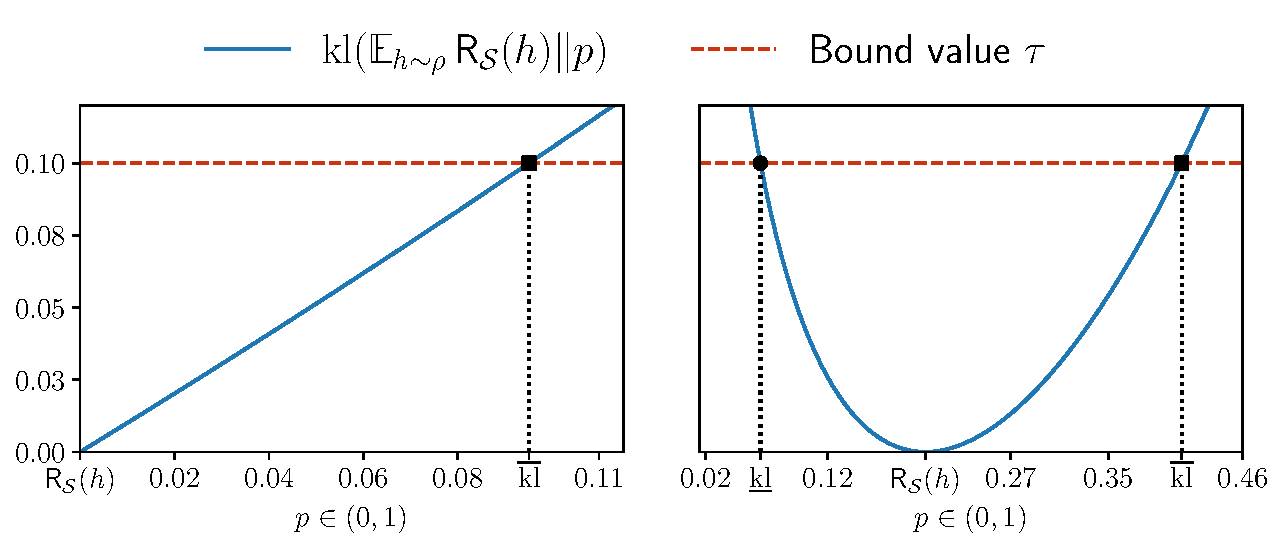
\includegraphics[width=\textwidth]{chapter_2/figures/invert_kl_optim.pdf}
    \caption[Illustration of the Functions $\klmin$ and $\klmax$]{%
    Illustration of the inverting functions of $\kl()$ for $q=\RiskLoss_{\dS}(\h)$ \st $\RiskLoss_{\dS}(\h) \in \{0.0, 0.2\}$ in two different plots.
    We plot the curve of the function $\kl(\RiskLoss_{\dS}(\h)\|\cdot)$, the bound value $\threshold=0.1$ and the two inverting functions $\klmin(\RiskLoss_{\dS}(\h)| \threshold)$ and $\klmax(\RiskLoss_{\dS}(\h)| \threshold)$ (abbreviated $\klmin$ and $\klmax$).
    The dot (\resp the square) corresponds to the solution of the minimization (\resp maximization) problem associated with $\klmin$ (\resp $\klmax$).
    }
    \label{chap:pac-bayes:fig:invert-kl-optim}
\end{figure}
Expressed as it is,  \Cref{chap:pac-bayes:eq:seeger} does not permit to upper or lower bound the expected true risk $\RiskLoss_{\D}(\h)$ contrary to \Cref{chap:pac-bayes:theorem:mcallester,chap:pac-bayes:theorem:catoni}.
In order to rewrite \Cref{chap:pac-bayes:eq:seeger} (of \Cref{chap:pac-bayes:theorem:seeger}), we define the inverting functions of $\kl()$ in the following way. 

\begin{definition}[Inverting Functions of $\kl()$] Given $\threshold\ge 0$, for any $q\in[0, 1]$, the inverting functions of the $\kl()$ are defined as
\begin{align*}
    &\klmax(q | \threshold){\defeq}\max\Big\{ p \in (0,1) \;\Big|\; \kl(q\|p) \le \threshold\Big\},\\ 
    \text{and}\quad &\klmin (q | \threshold){\defeq}\min\Big\{ p\!\in\!(0,\! 1) \;\Big|\; \kl(q\|p) \le\threshold\Big\}.
\end{align*}
\label{chap:pac-bayes:def:invert-kl}
\end{definition}

The function $\klmax()$ (\resp $\klmin()$) denotes the maximum (\resp minimum) value $p\in(0,1)$ such that the inequality $\kl(q\|p) \le \threshold$ holds.
\Cref{chap:pac-bayes:fig:invert-kl-optim} gives a graphical illustration of these inverting functions.
The values associated with the inverting functions $\klmin()$ and $\klmax()$ can be approximated and easily computed from \textsc{Pinsker}'s inequality (\Cref{ap:pac-bayes:theorem:pinsker}).
Indeed, we have
\begin{align}
    \klmax(q|\threshold) \le q + \sqrt{\frac{1}{2}\threshold} \qquad\text{and}\qquad q - \sqrt{\frac{1}{2}\threshold} \le \klmin(q|\threshold).\label{chap:pac-bayes:eq:kl-approx}
\end{align}
We present in \Cref{chap:pac-bayes:fig:invert-kl-pinsker} an illustration of the tightness of this approximation.

\begin{figure}[t]
    \centering
    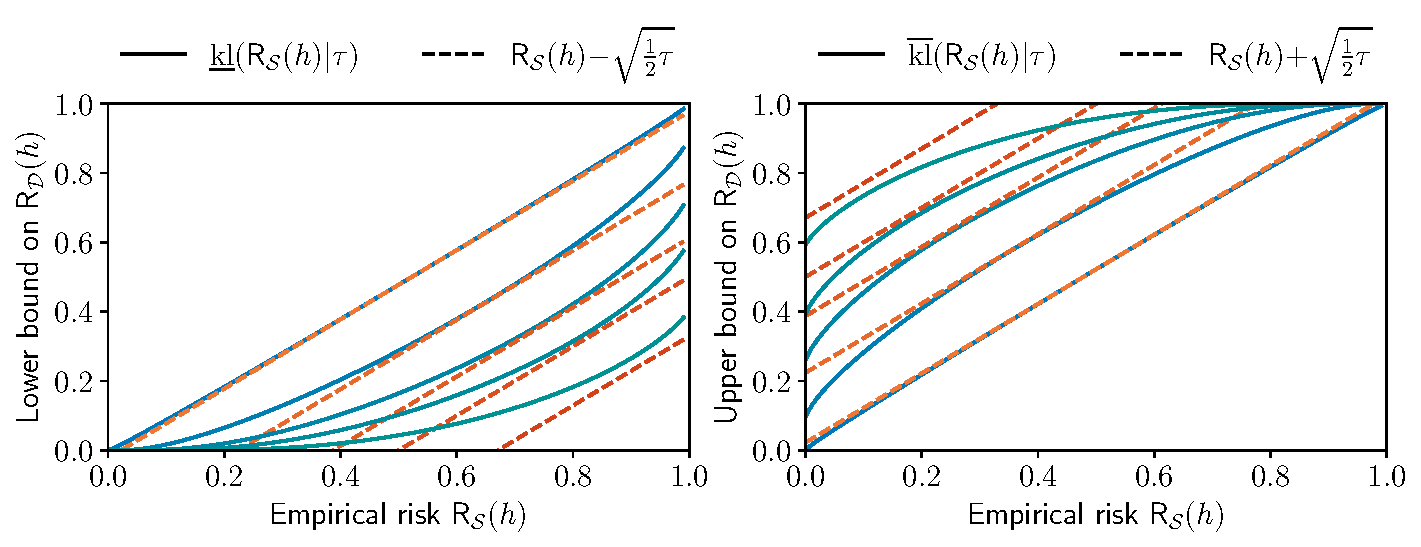
\includegraphics[width=\textwidth]{chapter_2/figures/invert_kl_pinsker.pdf}
    \caption[Illustration of the Tightness of $\klmin$ and $\klmax$]{%
    Illustration of the tightness of $\klmin()$ and $\klmax()$.
    The line represents the functions $\klmin(\cdot|\threshold)$ and $\klmax(\cdot|\threshold)$ for different values of $\threshold\in\{0.001, 0.1, 0.3, 0.5, 0.9\}$.
    On the left plot, we represent the function $\klmin(\cdot|\threshold)$ while the right plot represents the function $\klmax(\cdot|\threshold)$. 
    In the left (\resp right) plot, the lower (\resp higher) the inverting function, the smaller (\resp larger) the value of $\threshold$.
    Moreover, for each inverting function, we plot with the dotted lines its approximation through \textsc{Pinsker}'s inequality.
    }
    \label{chap:pac-bayes:fig:invert-kl-pinsker}
\end{figure}

To calculate $\klmin()$ and $\klmax()$ exactly, two optimization problems need to be solved; \citet{ReebDoerrGerwinnRakitsch2018} proposed an algorithm based on the bisection method.
We recall its pseudo-code in \Cref{chap:pac-bayes:algo:kl}. 
The principle of this algorithm is to iteratively refine the interval $[p_{\text{min}}, p_{\text{max}}]$ to which the bias $p\in(0,1]$ belongs.
When the equality $\kl(q\|p)=\threshold$ is attained or when the interval $[p_{\text{min}}, p_{\text{max}}]$ is small enough, the bias $p$ is found.

\begin{algorithm}[ht!]
   \caption{Compute $\klmax(q|\threshold)$ \resp $\klmin(q|\threshold)$ through the bisection method}
  \begin{algorithmic}
    \State{{\bf Given: } Bias $q\in[0,1]$ (the empirical risk), the bound value $\threshold\ge 0$}
    \State{{\bf Hyperparameters: } tolerance $\epsilon$, maximal number of iterations $T_\text{max}$}
    \State{$p_{\text{max}}{\leftarrow}1$ and $p_{\text{min}}{\leftarrow}q$ (resp. $p_{\text{max}}{\leftarrow}q$ and $p_{\text{min}}{\leftarrow}0$)}
    \For{$t\leftarrow 1$ to $T_{\text{max}}$}
        \State{$p = \tfrac{1}{2}\LB p_{\text{min}}{+}p_{\text{max}}\RB$}
        \State{\textbf{if} $\kl(q\|p)=\threshold$ or  $(p_{\text{min}}{-}p_{\text{max}})<\epsilon$ \textbf{ then return} $p$}
        \State{\textbf{if} $\kl(q\|p) > \threshold$ \textbf{ then } $p_\text{max}=p$ (resp. $p_\text{min}=p$)}
        \State{\textbf{if} $\kl(q\|p) < \threshold$ \textbf{ then } $p_\text{min}=p$ (resp. $p_\text{max}=p$)}
    \EndFor
     \State{\Return{$p$}}
    \end{algorithmic}
    \label{chap:pac-bayes:algo:kl}
\end{algorithm}

Moreover, \citet{ReebDoerrGerwinnRakitsch2018} found the expression of the derivatives with respect to $q$ and $\threshold$, allowing them to derive bound minimization algorithms based on gradient descent; these derivatives are defined by
\begin{align}
    \frac{\partial {\rm k(}q|\psi)}{\partial q} = \frac{\ln\frac{1-q}{1-{\rm k(}q|\psi)}-\ln\frac{q}{{\rm k(}q|\psi)}}{\frac{1-q}{1-{\rm k(}q|\psi)}-\frac{q}{{\rm k(}q|\psi)}}, \text{ and } \frac{\partial {\rm k(}q|\psi)}{\partial \psi} = \frac{1}{\frac{1-q}{1-{\rm k(}q|\psi)}-\frac{q}{{\rm k(}q|\psi)}},\label{chap:pac-bayes:eq:deriv-kl}
\end{align}
where ${\rm k}()$ is either $\klmin()$ or $\klmax()$.

Thanks to \Cref{chap:pac-bayes:def:invert-kl}, we can rewrite the bound of \Cref{chap:pac-bayes:theorem:seeger} to upper-bound the expected true risk $\EE_{\h\sim\Q}\RiskLoss_{\D}(\h)$.
With probability at least $1-\delta$ over the random choice of $\S\sim\D^\m$, we have for all $\Q\in\M(\H)$
\begin{align}
    &\EE_{\h\sim\Q}\RiskLoss_{\D}(\h) \le \klmax\LP\EE_{\h\sim\Q}\RiskLoss_{\dS}(\h) \;\middle|\; \frac{1}{\m}\!\LB\KL(\Q\|\P){+}\ln\tfrac{2\sqrt{\m}}{\delta}\RB\RP\label{chap:pac-bayes:eq:klmax-seeger}\\
    \text{and}\quad &\EE_{\h\sim\Q}\RiskLoss_{\D}(\h) \ge \klmin\LP\EE_{\h\sim\Q}\RiskLoss_{\dS}(\h) \;\middle|\; \frac{1}{\m}\!\LB\KL(\Q\|\P){+}\ln\tfrac{2\sqrt{\m}}{\delta}\RB\RP.\label{chap:pac-bayes:eq:klmin-seeger}
\end{align}

Thanks to the approximation in \Cref{chap:pac-bayes:eq:kl-approx}, one can prove that the bound of \Cref{chap:pac-bayes:theorem:seeger} is tighter than the one of \Cref{chap:pac-bayes:theorem:mcallester}.
More precisely, if we apply \Cref{chap:pac-bayes:eq:kl-approx} to \Cref{chap:pac-bayes:eq:klmax-seeger,chap:pac-bayes:eq:klmin-seeger}, we retrieve \Cref{chap:pac-bayes:eq:mcallester-1,chap:pac-bayes:eq:mcallester-2}.


\subsection{General PAC-Bayesian Bound of \citet{BeginGermainLavioletteRoy2016}}

As shown previously, the KL divergence between the posterior distribution $\Q$ and the prior distribution $\P$ is ubiquitous in PAC-Bayesian bounds.
By considering this divergence, as illustrated in \Cref{chap:pac-bayes:theorem:general-germain}, the term $\EE_{\S'\sim\D^\m}\EE_{\h'\sim\P}\exp\LB\varphi(\h', \S')\RB$ appears inevitably.
Indeed, the KL divergence $\KL(\Q\|\P)$ between $\Q$ and $\P$ can be expressed as a difference between two terms: $\EE_{\h\sim\Q}\varphi(\h,\S)$ and $\EE_{\h\sim\P}\exp\LB\varphi(\h, \S)\RB$ thanks to \citet{DonskerVaradhan1976}.
This representation is actually used to obtain a {\it change of measure inequality} which quantifies how much two expectations (coming from two densities $\Q$ and $\P$) differ.
This change of measure inequality and the expression of the KL divergence are in the following.

\begin{restatable}[\mbox{\textsc{Donsker}-\textsc{Varadhan} Variational Representation}]{proposition}{representationKL}\label{chap:pac-bayes:proposition:representation-KL}
For any hypothesis set $\H$, for any distribution $\P\in\M^{*}(\H)$ on $\H$, for any measurable function $\varphi:\H\times(\X\times\Y)^\m \rightarrow \Rbb$ \st $\EE_{\h'\sim\P}e^{\varphi(\h',\S)}<+\infty$ for all $\S\in(\X\times\Y)^\m$, we have
\begin{align*}
    \forall\S\in(\X\times\Y)^\m,\quad \forall\Q\in\M(\H),\qquad 
    &\EE_{\h\sim\Q}\varphi(\h,\S)-\ln\LP \EE_{\h\sim\P}e^{\varphi(\h,\S)}\RP \le \KL(\Q\|\P)\\
    \iff &\EE_{\h\sim\Q}\varphi(\h,\S) \le \KL(\Q\|\P)+\ln\LP \EE_{\h\sim\P}e^{\varphi(\h,\S)}\RP.
\end{align*}

When the distribution $\Q$ is defined as $\displaystyle\Q(\h)=\P(\h)\frac{e^{\varphi(\h,\S)}}{\EE_{\h'\sim\P}e^{\varphi(\h',\S)}}$, we have
\begin{align*}
    \forall\S\in(\X\times\Y)^\m,\qquad &\EE_{\h\sim\Q}\varphi(\h,\S)-\ln\LP \EE_{\h\sim\P}e^{\varphi(\h,\S)}\RP = \KL(\Q\|\P), \\
    \iff &\EE_{\h\sim\Q}\varphi(\h,\S) = \KL(\Q\|\P)+\ln\LP \EE_{\h\sim\P}e^{\varphi(\h,\S)}\RP.
\end{align*}
\end{restatable}
\begin{noaddcontents}\begin{proof}
Deferred to~\Cref{ap:pac-bayes:sec:proof-representation-KL}.
\end{proof}\end{noaddcontents}

As we can remark, this inequality resembles to the general bound of \citet{GermainLacasseLavioletteMarchand2009} (in \Cref{chap:pac-bayes:theorem:general-germain}).
Hence, the change of measure inequality appears indirectly in the PAC-Bayesian bounds making the constant term $\EE_{\S'\sim\D^\m}\EE_{\h'\sim\P}e^{\varphi(\h',\S')}$ arising in the bound.
Other divergences can be considered to obtain different constant terms (that are further upper-bounded).
For example, \citet{OhnishiHonorio2021} prove other change of measure inequalities for several divergences.
Prior to this work, \citet{BeginGermainLavioletteRoy2016} derive a new general PAC-Bayesian bound with the \textsc{Rényi} divergence defined as $\Renyi_{\lambda}(\Q\|\P) = \frac{1}{\lambda{-}1}\ln\LP\EE_{\h\sim\P}\LB\frac{\Q(\h)}{\P(\h)}\RB^\lambda\RP$ for any $\lambda> 1$.
Their bound is recalled in the following theorem.

\begin{restatable}[General PAC-Bayesian Bound of~\citet{BeginGermainLavioletteRoy2016}]{theorem}{generalbegin}\label{chap:pac-bayes:theorem:general-begin}
For any distribution $\D$ on $\X{\times}\Y$, for any hypothesis set $\H$, for any distribution $\P\in\M^{*}(\H)$ on $\H$, for any measurable function $\varphi: \H\times(\X\times\Y)^\m\to \Rbb_{*}^{+}$, for any $\lambda > 1$, for any $\delta\in(0,1]$, we have
\begin{align*}
&\PP_{\S\sim\D^{\m}}\Bigg[ \forall \Q\in\M(\H), \frac{\lambda}{\lambda{-}1}
   \ln \LB\EE_{\h{\sim}\Q}\varphi(\h,\S)\RB\\
&\hspace{3cm}\le \Renyi_{\lambda}(\Q\|\P) + \ln\LB\frac{1}{\delta}\EE_{\S'{\sim}\D^{\m}}\EE_{\h'{\sim}\P}\varphi(\h',\S')^\frac{\lambda}{\lambda{-}1}\RB \Bigg] \ge 1{-}\delta.
\end{align*}
\end{restatable}
\begin{noaddcontents}\begin{proof}
Deferred to~\Cref{ap:pac-bayes:sec:proof-general-begin}.
\end{proof}\end{noaddcontents}

Unlike \Cref{chap:pac-bayes:theorem:general-germain}, the function $(\h,\S) \mapsto \frac{\lambda}{\lambda{-}1}\ln \LB\EE_{\h{\sim}\Q}\varphi(\h,\S)\RB$ represents the generalization gap and is upper-bounded by the \textsc{Rényi} divergence $\Renyi_{\lambda}(\Q\|\P)$ and a constant term $\ln[\frac{1}{\delta}\EE_{\S'{\sim}\D^{\m}}\EE_{\h'{\sim}\P}\varphi(\h',\S')^\frac{\lambda}{\lambda{-}1}]$.
At first sight, \Cref{chap:pac-bayes:theorem:general-begin} seems very different from \Cref{chap:pac-bayes:theorem:general-germain}, however, they are actually related.
Indeed, if we replace $\varphi(\h,\S)$ by $\exp(\tfrac{\lambda{-}1}{\lambda}\varphi(\h,\S))$ and we apply \textsc{Jensen}'s inequality (\Cref{ap:tools:theorem:jensen}) on the left-hand side, we obtain with probability at least $1{-}\delta$ over the random choice of $\S{\sim}\D^\m$
\begin{align*}
    \forall \Q\in\M(\H),\quad \EE_{\h\sim\Q}\varphi(\h,\S) \le \Renyi_{\lambda}(\Q\|\P) + \ln\LB\frac{1}{\delta}\EE_{\S'{\sim}\D^{\m}}\EE_{\h'{\sim}\P}e^{\varphi(\h',\S')} \RB.
\end{align*}

This bound is slightly looser than the one of \Cref{chap:pac-bayes:theorem:general-germain}: for any $\lambda>1$ and for any distributions $\Q$ and $\P$, we have $\KL(\Q\|\P) \le \Renyi_{\lambda}(\Q\|\P)$ and $\lim_{\lambda\rightarrow 1^{+}}\Renyi_{\lambda}(\Q\|\P)=\KL(\Q\|\P)$ \citep{ErvenHarremoes2014}.
As for the general bound in \Cref{chap:pac-bayes:theorem:general-germain}, setting the function $\varphi()$ and upper-bounding the term $\EE_{\S{\sim}\D^{\m}}\EE_{\h{\sim}\P}\varphi(\h,\S)^\frac{\lambda}{\lambda{-}1}$ gives a computable bound.
Namely, \Cref{chap:pac-bayes:theorem:general-begin} allows one to obtain a \citeauthor{McAllester2003}, \citeauthor{Catoni2007} or a \citeauthor{Seeger2002}-like PAC-Bayesian bound based on the \textsc{Rényi} divergence.
For the sake of completeness, we show in \Cref{ap:pac-bayes:sec:corollary-begin} the proof of the three types of bounds based on \Cref{chap:pac-bayes:theorem:general-begin}.
Compared to \Cref{chap:pac-bayes:theorem:mcallester,chap:pac-bayes:theorem:catoni,chap:pac-bayes:theorem:seeger}, only the KL divergence is replaced by the looser \textsc{Rényi} divergence.\\

Generally speaking, all the PAC-Bayesian bounds share a common property: they bound the {\it expectation} of $\varphi()$ \wrt the posterior $\Q$.
However, it might be relevant to upper-bound $\varphi()$ for a {\it unique} hypothesis $\h\sim\Q$: this is the purpose of the {\it disintegrated} bounds.

\section{Disintegrated PAC-Bayesian Bounds}
\label{chap:pac-bayes:sec:disintegrated}

Deriving PAC-Bayesian guarantees for a unique hypothesis is tedious.
Indeed, the PAC-Bayesian theory is tailored for bounding the {\it expected} true risk.
Hence, additional derivations are needed to derive a PAC-Bayesian guarantee for a unique hypothesis.
See \citet{Langford2005,LangfordShaweTaylor2002,GermainLacasseLavioletteMarchand2009} for some examples.
To avoid this issue and to get a bound for a single hypothesis, another possible solution is to sample the hypothesis $\h\in\H$ from the posterior distribution $\AQ \in \M(\H)$.
By doing so, the gap $\LN \RiskLoss_{\D}(\h)-\RiskLoss_{\dS}(\h)\RN$ can be upper-bounded with a generalization bound.
This bound is defined in the following way.

\begin{restatable}[Disintegrated PAC-Bayesian Generalization Bound]{definition}{definitiondesintegrated}\label{chap:pac-bayes:def:disintegrated-pac-bayes}
Let $\loss: \H \times(\X{\times}\Y)\rightarrow [0,1]$ be a loss function and $\phi: [0,1]^2{\to}[0,1]$ a generalization gap. 
A {\it disintegrated} PAC-Bayesian bound is defined such that if for any distribution $\D$ on $\X\times\Y$, for any hypothesis set $\H$, for any prior distribution $\P\in\M^{*}(\H)$, for any algorithm \mbox{$A\!:\!(\X{\times}\Y)^{\m}{\times}\M^{*}(\H){\to} \M(\H)$}, there exists a function $\Phi: \M(\H){\times}\M^{*}(\H){\times}(0,1]{\to} \Rbb$ such that for any $\delta\in(0, 1]$ we have
\begin{align*}
    \PP_{\S\sim\D^\m, \h\sim\AQ}\LB \phi(\RiskLoss_{\D}(\h), \RiskLoss_{\dS}(\h)) \le \Phi\big(\AQ, \P, \delta\big) \RB \ge 1-\delta,
\end{align*}
where $\AQ \defeq A(\S, \P)$ is output by the deterministic algorithm $A$ and $\phi()$ is, for example, $\phi(\RiskLoss_{\D}(\h), \RiskLoss_{\dS}(\h)) = \LN\RiskLoss_{\D}(\h)-\RiskLoss_{\dS}(\h)\RN$.
\end{restatable}


Compared to the PAC-Bayesian bounds (see \Cref{chap:pac-bayes:def:pac-bayes}), the expectation $\EE_{\h\sim\AQ}\LB\cdot\RB$ is moved outside the indicator function: this is the disintegration.
Moreover, unlike the PAC-Bayesian bounds, the posterior $\AQ$ is obtained from an algorithm that depends on the prior $\P\in\M^{*}(\H)$ and the learning sample $\S$.
This type of bounds has been introduced in two concurrent works, \ie, \citet[Theorem~1.2.7]{Catoni2007} and \citet{BlanchardFleuret2007}.
Moreover, there exists a general disintegrated bound as for the PAC-Bayesian bounds.
We now present these three bounds by starting with the most general one.

\subsection{General Disintegrated Bound of \citet{RivasplataKuzborskijSzepesvariShaweTaylor2020}}

A general disintegrated PAC-Bayesian bound has been actually proposed very recently by \citet[Theorem~1-(i)]{RivasplataKuzborskijSzepesvariShaweTaylor2020}. 
This bound is presented below.

\begin{restatable}[General Disintegrated Bound of~\citet{RivasplataKuzborskijSzepesvariShaweTaylor2020}]{theorem}{generaldisintegratedrivasplata}\label{chap:pac-bayes:theorem:general-disintegrated-rivasplata}
For any distribution $\D$ on $\X\times\Y$, for any hypothesis set $\H$, for any prior distribution $\P\in\M^{*}(\H)$, for any measurable function $\varphi: \H\times(\X\times\Y)^\m\to \Rbb$, for any $\delta\in(0, 1]$, for any algorithm \mbox{$A\!:\!(\X{\times}\Y)^{\m}{\times}\M^{*}(\H){\to} \M(\H)$}, we have
\begin{align*}
\PP_{\S\sim\D^\m, \h\sim\AQ}\Bigg[ \varphi(\h,\S) \le \underbrace{\ln\!\LB\frac{\AQ(\h)}{\P(\h)}\RB\!+\!\ln\!\LB\frac{1}{\delta}\EE_{\S'\sim\D^\m}\EE_{\h'\sim\P}
\exp\LP\varphi(\h',\S')\RP\RB}_{\Phi(\AQ, \P, \delta)}
\Bigg] \ge 1{-}\delta,
\end{align*}
where $\AQ \defeq A(\S, \P)$ is output by the deterministic algorithm $A$.
\end{restatable}
\begin{noaddcontents}\begin{proof}
Deferred to~\Cref{ap:pac-bayes:sec:proof-general-disintegrated-rivasplata}.
\end{proof}\end{noaddcontents}

Compared to the classical PAC-Bayesian bounds, this bound holds with high probability over the random choice of the learning sample $\S\sim\D^\m$ {\it and} the hypothesis $\h\sim\AQ$.
Moreover, instead of depending on the KL divergence, the bound depends on the {\it disintegrated} KL divergence\footnote{The disintegration of the KL divergence has a slightly different meaning than the disintegration of the PAC-Bayesian bound: in the former case, the integration/expectation ``is removed'' from the divergence.} $\ln\frac{\AQ(\h)}{\P(\h)}$.
This term is the log ratio of the density of the prior $\P(\h)$ and the posterior distribution $\AQ(\h)$ for the sampled hypothesis $\h\sim\AQ$.
Intuitively, the closer the posterior density $\AQ(\h)$ to the prior density $\P(\h)$ for $\h\sim\AQ$, the lower the disintegrated KL.
As for \citet{GermainLacasseLavioletteMarchand2009}'s general bound, we need to define $\varphi()$ and upper-bound the term $\EE_{\S'\sim\D^\m}\EE_{\h'\sim\P}
\exp\LP\varphi(\h',\S')\RP$ to obtain a bound that can be computed.
Similarly to \Cref{chap:pac-bayes:theorem:general-germain,chap:pac-bayes:theorem:general-begin}, this disintegrated bound generalizes other bounds such as the one derived by \citet[Theorem~1.2.7]{Catoni2007}.

\subsection{Disintegrated Bound of \citet{Catoni2007}}

The bound of \citet[Theorem 1.2.7]{Catoni2007}, which is one of the first disintegrated bound in the literature, is recalled in the following theorem.

\begin{restatable}[Disintegrated Bound of \citet{Catoni2007}]{theorem}{disintegratedcatoni}\label{chap:pac-bayes:theorem:disintegrated-catoni}
For any distribution $\D$ on $\X\times\Y$, for any hypothesis $\H$, for any prior $\P\in\M^{*}(\H)$, for any loss $\loss: \H{\times}(\X\times\Y)^\m \to [0, 1]$, for any $\cat>0$, for any $\delta\in(0, 1]$, for any algorithm \mbox{$A\!:\!(\X{\times}\Y)^{\m}{\times}\M^{*}(\H){\to} \M(\H)$}, we have
\begin{align*}
    \PP_{\S\sim\D^\m,\h\sim\AQ}\Bigg[ \forall\Q\in\M(\H), 
    -\ln\!\LP 1{-}\LB1{-}e^{{-}\cat}\RB\EE_{\h\sim\Q}\RiskLoss_{\D}(\h)\RP&-\cat\EE_{\h\sim\Q}\RiskLoss_{\dS}(\h)\\
    &\hspace{-2cm}\le \frac{1}{\m}\LB\ln\frac{\AQ(\h)}{\P(\h)}{+}\ln\frac{1}{\delta}\RB\Bigg] \ge 1-\delta,
\end{align*}
where $\AQ \defeq A(\S, \P)$ is output by the deterministic algorithm $A$.
\end{restatable}
\begin{noaddcontents}\begin{proof}
Deferred to~\Cref{ap:pac-bayes:sec:proof-disintegrated-catoni}.
\end{proof}\end{noaddcontents}

After sampling the learning sample $\S\sim\D^\m$ and the hypothesis $\h\sim\AQ$, the obtained guarantee is similar to the one of \Cref{chap:pac-bayes:theorem:catoni}: only the KL divergence is replaced by its disintegrated counterpart.
Similar to the non-disintegrated PAC-Bayesian bound, other deviations between the true risk $\RiskLoss_{\D}(\h)$ and the empirical risk $\RiskLoss_{\dS}(\Q)$ can be considered.
For instance, \citet{BlanchardFleuret2007} proposed a bound on $\kl(\RiskLoss_{\dS}(\h)\|\RiskLoss_{\D}(\h))$. 

\subsection{Disintegrated Bound of \citet{BlanchardFleuret2007}}

The bound of \citet{BlanchardFleuret2007} is based on another proof technique called {\it Occam's hammer}.
For instance, they prove a \citet{Seeger2002}-like disintegrated PAC-Bayesian bound from this framework; it is recalled in the following theorem.

\begin{restatable}[Disintegrated Bound of \citet{BlanchardFleuret2007}]{theorem}{disintegratedblanchard}\label{chap:pac-bayes:theorem:disintegrated-blanchard}
For any distribution $\D$ on $\X\times\Y$, for any hypothesis set $\H$, for any distribution $\P\in\M^{*}(\H)$, for any loss $\loss: \H\times(\X\times\Y)\to \{0,1\}$, for any $\blan>1$, for any $\delta\in(0, 1]$, for any algorithm \mbox{$A\!:\!(\X{\times}\Y)^{\m}{\times}\M^{*}(\H){\to} \M(\H)$}, we have
\begin{align*}
\PP_{\S\sim\D^\m, \h\sim\AQ}\LB \kl_{+}(\RiskLoss_{\dS}(\h)\|\RiskLoss_{\D}(\h)) \le  \frac{1}{\m}\LB\ln\frac{\blan+1}{\delta}+\LP1+\frac{1}{\blan}\RP\ln_{+}\frac{\AQ(\h)}{\P(\h)}\RB \RB \ge 1-\delta,
\end{align*}
where $\AQ \defeq A(\S, \P)$ is output by the deterministic algorithm $A$, the $\ln_{+}(x)=\max(\ln(x), 0)$ and $\kl_{+}(\RiskLoss_{\dS}(\h)\|\RiskLoss_{\D}(\h))=\kl(\RiskLoss_{\dS}(\h)\|\RiskLoss_{\D}(\h))$ if $\RiskLoss_{\dS}(\h)<\RiskLoss_{\D}(\h)$ and 0 otherwise.
\end{restatable}
\begin{noaddcontents}\begin{proof}
Deferred to~\Cref{ap:pac-bayes:sec:proof-disintegrated-blanchard}.
\end{proof}\end{noaddcontents}

Similarly to \citet{Catoni2007}, this bound is parametrized: the tightness depends on the parameter $\blan>1$.
However, the optimal parameter depends on the log ratio $\ln_{+}\frac{\AQ(\h)}{\P(\h)}$ and cannot be set in advance since we don't know the sampled $\S\sim\D^\m$.

\section{Conclusion and Summary}

This chapter introduces generalization bounds from the PAC-Bayesian literature.
These bounds allow deriving theoretical guarantees for some machine learning models, \eg, the majority vote.
They are further useful to derive practical learning algorithms guaranteeing that the model is not too sensitive to overfitting; see \Cref{part:contrib-pac-bayes}.
Indeed, in \Cref{chap:mv-robustness}, we derive a new self-bounding learning algorithm that minimizes a PAC-Bayesian generalization bound for the adversarially robust setting.
Roughly speaking, we derive surrogates similar to \Cref{chap:pac-bayes:eq:2gibbs} to obtain guarantees and derive learning algorithms that ``robustify'' the majority vote.
Then, \Cref{chap:mv} introduces our contributions to minimizing of the PAC-Bayesian C-Bound, which aims to minimize the true risk of the majority vote.
Lastly in \Cref{part:contrib-pac-bayes}, we introduce the stochastic majority vote (where the distribution $\Q$ follows a Dirichlet distribution) in \Cref{chap:mv-sto}. 
This majority vote allows using easily a PAC-Bayesian bound on the expected true risk to learn such a classifier.\\

However, the main drawback of the PAC-Bayesian generalization bounds is that we bound $\EE_{\h\sim\Q}\varphi(h,\S)$ instead of $\varphi(h,\S)$.
In contrast, the disintegrated bounds allow us to bound the term $\varphi(h,\S)$, which makes more sense if we want to deal with a unique hypothesis $h\sim\Q$.
\Cref{part:contrib-disintegrated} shows the potential of such bounds for the analysis of the generalization of over-parametrized models.
Indeed, \Cref{chap:dis-pra} shows the first application of such bounds in practice, notably with over-parametrized models; this also leads to the derivation of new disintegrated bounds that are more appealing to optimization.
Lastly, \Cref{chap:dis-mu} introduces new perspectives based on these bounds since we can derive generalization bounds that do not depend on classical complexity measures such as the VC-Dimension or the Rademacher complexity (see \Cref{chap:intro:sec:bound}).

% ----------------------------------------------------------------------------------------------- %

\part[PAC-Bayesian Majority Vote:\\ Theory and Self-bounding Algorithms]{PAC-Bayesian Majority Vote:\\ {\LARGE Theory and Self-bounding Algorithms}}
\label{part:contrib-pac-bayes}

%\chapter[Mitigating Initialisation Impact by Real-Time Control: Online PAC-Bayes Learning]{Mitigating Initialisation Impact by Real-Time Control: Online PAC-Bayes Learning}
\label{chap:online-pb}

\addchapterlof
\addchapterloa
\addchapterloe

\vspace{-1.0cm}
\begin{center}
\textbf{This chapter is based on the following papers}\\[0.1cm]
\end{center}
\printpublication{haddouche2022online}
\\
\printpublication{haddouche2023pac}
\\
\printpublication{viallard2023learning}

\vspace{0.2cm}
\minitoc

\begin{abstract}
Put OPB here. Precise in the intro that the martingale bounds allow to go beyond batch learning but that this has never been made for OL. Put the supermartingale OPB bound in a supplementary section and the Online WPB bound after the main results of OPB to reach heavy-tailed losses. 
\end{abstract}


\section{Online PAC-Bayes learning beyond bounded losses.}
\label{sec: main_result_onl}

Recently, an online learning framework has been designed in \citet{haddouche2022online}. This allowed the design of Online PAC-Bayes (OPB) algorithms which involved the use of history-dependent priors evolving at each time step of the learning procedure. The main contribution of this section is an OPB bound valid for unbounded losses.

\paragraph{Framework} We consider the same framework as in \Cref{sec: iid_case} except we do not make any assumption on the data distribution. Our goal is now to define a posterior sequence $(\Q_i)_{i\geq 1}$ from a prior sequence $(\P_i)_{i\geq 1}$. We also define a filtration $(\mathcal{F}_{i})_{i\geq 1}$ adapted to $(z_i)_{i\geq 1}$. We reuse the following definitions extracted from \cite{haddouche2022online}.

\paragraph{Definitions} For all $i$, we denote by $\mathbb{E}_{i}[.]$ the conditional expectation $\mathbb{E}[.\mid \mathcal{F}_i]$.

A \emph{stochastic kernel} from $\cup_{m=1}^\infty\mathcal{Z}^m$ to $\mathcal{H}$ is defined as a mapping $Q: \cup_{m=1}^\infty\mathcal{Z}^m\times \Sigma_{\mathcal{H}} \rightarrow [0,1]$ where
(i) For any $B\in \Sigma_{\mathcal{H}}$, the function  $S\mapsto Q(S,B)$ is measurable,  (ii) For any $\S$, the function $B\mapsto Q(S,B)$ is a probability measure over $\mathcal{H}$.


We also say that a sequence of stochastic kernels $(P_i)_{i\geq 1}$ is an \emph{online predictive sequence} if (i) for all $i\geq 1, S\in\cup_{m=1}^\infty\mathcal{Z}^m, P_i(S,.)$ is $\mathcal{F}_{i-1}$ measurable and (ii) for all $i \geq 2$, $P_i(S,.)\gg P_{1}(S,.)$.

\textbf{Main result.} We now state the main theorem of this section, which extends the remits of the Online PAC-Bayes framework to the case of unbounded losses.

\begin{theorem}
  \label{th: main_thm_onl}
  For any distribution over the (countable) dataset $\S$, any $\lambda>0$ and any online predictive sequence (used as priors) $(P_i)_{i\geq 1}$, we have with probability at least $1-\delta$ over the sample $S\sim\mu$, the following, holding for the data-dependent measures $P_{i,S}:= P_i(S,.)$ any posterior sequence $(Q_i)_{i\geq 1}$ and any $m\geq 1$:

  \begin{multline*}
     \sum_{i=1}^m \mathbb{E}_{h_i\sim Q_{i}}\left[ \mathbb{E}[\ell(h_i,z_i) \mid \mathcal{F}_{i-1}]    \right]  \leq \sum_{i=1}^m \mathbb{E}_{h_i\sim Q_{i}}\left[ \ell(h_i,z_i) \right] +\frac{\lambda}{2}\sum_{i=1}^m \mathbb{E}_{h_i\sim Q_i}\left[ \hat{V}_i(h_i,z_i) + V_i(h_i) \right] \\
     + \sum_{i=1}^m\frac{\operatorname{KL}(Q_{i}\| P_{i,S})}{\lambda}  + \frac{\log(1/\delta)}{\lambda}.
  \end{multline*}
  With for all $i$, $\hat{V}_i(h_i,z_i)= (\ell(h_i,z_i)-\mathbb{E}_{i-1}[\ell(h_i,z_i)])^2$ is the empirical variance at time $i$ and $V_i(h_i)= \mathbb{E}_{i-1}[\hat{V}(h_i,z_i)]$ is the true conditional variance.
\end{theorem}

Proof lies in \Cref{sec: proof_main_thm_online}.

\textbf{Analysis of the bound.} This bound is, to our knowledge, the first Online PAC-Bayes bound in literature holding for unbounded losses. It is semi-empirical as the variance and empirical variance terms have theoretical components. However, these terms can be controlled with assumptions on conditional second-order moments and not on exponential ones (as made in \citealp{haddouche2022online} where the bounded loss assumption was used to obtain conditional subgaussianity). To emphasise our point, we consider as in \Cref{sec: iid_case} the case of the quadratic loss $\ell(h,z)= (h-z)^2$. Here, we only need to assume that our data have a finite variance if we restrict our posteriors to have both bounded means and variance. Also the meaning of the online predictive sequence $P_i$ is that we must be able to design properly a sequence of priors before drawing our data, this can be for instance an online algorithm whihc generate a prior distribution from past data at each time step.

Finally, we note that if we assume being able to bound simultaneaously all condtional means and variance (which is strictly less restrictive than bounding the loss),then  \cref{th: main_thm_onl} suggests a new online learning objective which is an online counterpart to \Cref{eq: optim_obj}.

\begin{align}
    \forall i\geq1\; \hat{Q}_{i+1}&= \underset{Q\in\mathcal{M}^+_1(\mathcal{H})}{\mathrm{argmin}} \mathbb{E}_{h_i\sim Q} \; \left[\ell(h_i,z_i)+ \frac{\lambda}{2}\ell(h_i,z_i)^2\right] + \frac{\operatorname{KL}(Q\| P_{i,S})}{\lambda}
\end{align}

\textbf{Comparison with literature.} Our most natural comparison point is Theorem 2.3 of \cite{haddouche2022online} (re-stated in \cref{sec: pac_b_background}). We claim that \Cref{th: main_thm_onl} is a strict improvement of their result on various sides described below.

\begin{itemize}
  \item If we assume our loss to be bounded, then we can upper bound our empirical/theoretical variance terms to recover exactly \citet[][Theorem 2.3]{haddouche2022online}. Our bound can then be seen as a strict extension of theirs and shows that bounding order two moments is a sufficient condition to perform online PAC-Bayes: subgaussianity induced by boundedness is not necessary even when our data are non iid.
  \item Another crucial point lies on the range of our result which holds with high probability for any countable posterior sequence $(Q_i)_{i\geq 1}$, any time $m$ and the priors $(P_{i,S})_{i\geq 1}$.
  This is far much general than \citet[][Theorem 2.3]{haddouche2022online} which holds only for a single $m$ and a single posterior sequence $(Q_{i,S})_{i=1..m}$. This happens because in \citet{haddouche2022online}, the change of measure inequality has not been exploited: they used a preliminary theorem from \citet{rivasplata2020pac} which holds for a single (data-dependent) prior/posterior couple. This preliminary theorem already involved Markov's inequality which forced the authors to assume conditionnal subgaussianity to deal with an exponential moment. On the contrary, we exploited the fact that our online predictive sequence was history-dependent to use the change of measure inequality at any time step and control an exponential supermartingale through Ville's inequality.
  \item In \citet[Eq. 1]{haddouche2022online}, an OPB algorithm is given by their upper bound. This works because their associated learning objective admits a close form (Gibbs posterior) which matches the fact their bound hold for a single posterior sequence. Because our bound holds uniformly on all posteriors, it is now legitimate to restrict their algorithms to any parametric class of distributions and perform any optimisation algorithm to obtain a surrogate of the best candidate.
\end{itemize}

 Online PAC-Bayes as presented in \citet{haddouche2022online} relies on a conditional subgaussiannity assumption to control an exponential moment. They did not exploit a martingale-type structure to do so. Our supermartingale approach has proven to be well suited to Online PAC-Bayes as we provided atheorem valid for unbounded losses holding simultaneously on all posteriors: two points which have not been reached in \citet{haddouche2022online}.

\subsection{Proof of \Cref{th: main_thm_onl}}
\label{sec: proof_main_thm_online}
 \begin{proof}
   We fix $m\geq 1$, $\S$ a countable dataset and $(P_i)_{i\geq 1}$ an online predictive sequence. We aim to design a $m$-tuple of probabilities. Thus, our predictor set of interest is $\mathcal{H}_m:= \mathcal{H}^{\otimes m}$ and then, our predictor $h$ is a tuple $(h_1,..,h_m)\in\mathcal{H}$.

   Our goal is to apply the change of measure inequality on $\mathcal{H}_m$ to a specific function $f_m$ inspired from Lemma \ref{l: bercu_touati}. We define this function below, for any sample $\S$ and any predictor $h^m=(h_1,...,h_m)$

   \begin{align*}
   f_m(S,h^m) & := \sum_{i=1}^m \lambda X_i(h_i,z_i)  - \frac{\lambda^2}{2}\sum_{i=1}^m(\hat{V}_i(h_i,z_i) + V_i(h_i)),
   \end{align*}
   where $X_i(h_i,z_i)= \mathbb{E}_{i-1}[\ell(h_i,z_i)]- \ell(h_i,z_i)$. Notice that for fixed $h$, the sequence $(f_m(\S,h))_{m\geq 1}$ is a supermartingale according to Lemma \ref{l: bercu_touati}.

   Now for a given posterior tuple $Q_1,...Q_m$ we define $Q= Q_1 \otimes ...\otimes Q_m$ and also $P^m_S = P_{1,S}\otimes...\otimes P_{m,S}$. We can now properly apply the change of measure inequality for any $m$:
   \begin{align*}
    \sum_{i=1}^m \mathbb{E}_{h_i\sim Q_i}[\lambda X_i(h_i,z_i)  - \frac{\lambda^2}{2}(\hat{V}_i(h_i,z_i) + V_i(h_i))] & = \mathbb{E}_{h^m\sim Q}\left[ f_m(S,h^m) \right] \\
    & \leq \operatorname{KL}(Q,P^m_S) + \log \left( \mathbb{E}_{h^m\sim P^m_S}\exp(f_m(S,h^m))  \right).
   \end{align*}

   Noticing that $\operatorname{KL}(Q,P^m_S)= \sum_{i=1}^m \operatorname{KL}(Q_i,P_{i,S})$, the only remaining term to deal with is the exponential rv.

   To do so we prove the following lemma:

   \begin{lemma}
     The sequence $(M_m:=\mathbb{E}_{h^m\sim P^m_S}\exp(f_m(S,h^m))_{m\geq 1}$ is a non-negative supermartingale.
   \end{lemma}
   \begin{proof}
   We fix $m\geq 1$ and we recall that for any $i$, $P_{i,S}$ is $\mathcal{F}_{i-1}$-measurable. We show that $\mathbb{E}_{m-1}[M_m] \leq M_{m-1}$. We first recover $M_{m-1}$ from $\mathbb{E}_{m-1}[M_m]$.

     \begin{align*}
       \mathbb{E}_{m-1}[M_m]& =\mathbb{E}_{m-1}\left[\mathbb{E}_{h^m\sim P^m_S}\exp(f_m(S,h^m)\right] \\
       & = \mathbb{E}_{m-1}\left[\mathbb{E}_{h_1,..,h_m\sim P_{1,S}\otimes...\otimes P_{m,S}}\exp(f_m(S,h^m)\right] \\
       & = \mathbb{E}_{m-1}\left[\mathbb{E}_{h_1,..,h_m\sim P_{1,S}\otimes...\otimes P_{m,S}}\left[\Pi_{i=1}^m\exp\left(\lambda X_i(h_i,z_i)  - \frac{\lambda^2}{2}(\hat{V}_i(h_i,z_i) + V_i(h_i))\right)\right] \right] \\
        & = M_{m-1} \mathbb{E}_{m-1}\left[ \mathbb{E}_{h_m\sim P_{m,S}}\left[\exp\left(\lambda X_m(h_m,z_m)  - \frac{\lambda^2}{2}(\hat{V}_m(h_m,z_m) + V_m(h_m))\right) \right]\right].
     \end{align*}
 The last line holding because $P^{m-1}_S = P_{1,S}\otimes...\otimes P_{m-1,S}$ is $\mathcal{F}_{m-1}$ measurable.


   Now we exploit the fact that $P_{m,S}$ is $\mathcal{F}_{m-1}$ measurable to apply a conditional Fubini lemma stated in \citet[][Lemma D.3]{haddouche2022online}. We have:

   \begin{multline*}
     \mathbb{E}_{m-1}\left[ \mathbb{E}_{h_m\sim P_{m,S}}\left[\exp\left(\lambda X_m(h_m,z_m)  - \frac{\lambda^2}{2}(\hat{V}_m(h_m,z_m) + V_m(h_m))\right) \right]\right] \\ =  \mathbb{E}_{h_m\sim P_{m,S}}\left[\mathbb{E}_{m-1}\left[\exp\left(\lambda X_m(h_m,z_m)  - \frac{\lambda^2}{2}(\hat{V}_m(h_m,z_m) + V_m(h_m))\right) \right]\right].
   \end{multline*}

 Now we can apply Lemma \ref{l: bercu_touati} for any $h_m\in\mathcal{H}$ with $\Delta M_{m}=X_m(h_m,z_m), \Delta[M]_{m}=\hat{V}(h_m,z_m)$ and $\Delta\langle M\rangle_{m}= V_m(h_m)$. We then have for all $h_m\in\mathcal{H}$:

 \[ \mathbb{E}_{m-1}\left[\exp\left(\lambda X_m(h_m,z_m)  - \frac{\lambda^2}{2}(\hat{V}_m(h_m,z_m) + V_m(h_m))\right) \right] \leq 1.  \]

 Thus $\mathbb{E}_{m-1}[M_m] \leq M_{m-1}$, this concludes the lemma's proof.
   \end{proof}

 Now we can apply Ville's inequality which implies that with probability at least $1-\delta$, for any $m\geq 1$:

 \[ \mathbb{E}_{h^m\sim P^m_S}\exp(f_m(S,h^m)) \leq \frac{1}{\delta}. \]

 Thus we have with probability at least $1-\delta$, for any posterior sequence $(Q_i)_{i\geq 1}$, the data-dependent measures $P_{1,S},...,P_{m,S}$ and any $m\geq 1$:

 \begin{align*}
  \sum_{i=1}^m \mathbb{E}_{h_i\sim Q_i}\left[\lambda X_i(h_i,z_i)  - \frac{\lambda^2}{2}(\hat{V}_i(h_i,z_i) + V_i(h_i))\right] \leq \sum_{i=1}^m \operatorname{KL}(Q_i,P_{i,S}) + \log \left( \frac{1}{\delta}  \right).
 \end{align*}

 Re-organising the terms in this bound and dividing by $\lambda$ concludes the proof.

 \end{proof}

\newpage


%\chapter{Self-Bounding Algorithms for the Majority Vote}
\label{chap:mv}

\addchapterlof
\addchapterloa
\addchapterloe

\vspace{-1.5cm}
\begin{center}
\textbf{This chapter is based on the following paper}\\[0.1cm]
\end{center}
\printpublication{ViallardGermainHabrardMorvant2021}

\minitoc

\begin{abstract}
As we have seen in \Cref{chap:pac-bayes}, the C-Bound is an insightful upper bound on the risk of a majority vote classifier.
Learning algorithms in the literature minimize the empirical version of the C-Bound, instead of explicit PAC-Bayesian generalization bounds.
In this chapter, we derive self-bounding majority vote learning algorithms to directly optimize PAC-Bayesian guarantees on the C-Bound.
Our algorithms based on gradient descent are scalable and lead to accurate predictors paired with non-vacuous guarantees.
\end{abstract}

\newpage

\section{Introduction}

In this chapter, we introduce new learning algorithms for the majority vote in the context of supervised classification.
The goal of this algorithm is to minimize the true risk of the majority vote.
To do so, one way to minimize such a risk is to minimize the empirical C-Bound~\citep{Breiman2001,LacasseLavioletteMarchandGermainUsunier2006} introduced in \Cref{chap:pac-bayes:sec:surrogate} and estimated on the learning sample $\S$.
This bound has the advantage of involving the performance of the individual voters and the diversity in the voters' set. 
Indeed, these elements are important when one learns a  combination~\citep{Dietterich2000,Kuncheva2014}.
A good majority vote is made up of voters that are ``sufficiently diverse''.\\

Previous algorithms have been developed to minimize the {\it empirical} C-Bound such as \mincq \citep{RoyLavioletteMarchand2011}, \pmincq \citep{BelletHabrardMorvantSebban2014}, \cqboost \citep{RoyMarchandLaviolette2016}, or \cbboost \citep{BauvinCapponiRoyLaviolette2020}.
\citet{RoyLavioletteMarchand2011} first proposed \mincq which consist in minimizing a quadratic problem to learn a majority vote.
\mincq considers a specific voters' set to regularize the minimization process; the algorithm \pmincq generalizes \mincq by allowing prior distributions different from the uniform one.
One  drawback of \mincq and \pmincq is that the optimization problem is not scalable to large datasets.
Lately, \citet{BauvinCapponiRoyLaviolette2020} proposed \cbboost that minimizes in a boosting-based procedure with the advantage to be more scalable while obtaining sparser majority vote.
However, since both \mincq and \cbboost minimize the empirical C-Bound, the PAC-Bayesian generalization bound associated with their learned majority vote predictors can be vacuous.
Note that \cbboost has been proposed to improve another algorithm called  \cqboost~\citep{RoyMarchandLaviolette2016}.
Despite being empirically efficient and justified by theoretical analyses based on the C-Bound, all these methods minimize the empirical C-Bound and not directly a PAC-Bayesian generalization bound on the C-Bound.
This can lead to vacuous generalization bound values and, thus, to poor risk certificates.
When it comes to deriving a learning algorithm that directly minimizes a PAC-Bayesian bound, it is mentioned in the literature that optimizing a PAC-Bayesian bound on the C-bound is not trivial~\citep{MasegosaLorenzenIgelSeldin2020,LorenzenIgelSeldin2019}. 
This underlines the need for other majority vote learning algorithms based on the C-Bound, which motivates our contributions of \Cref{chap:mv:section:contribution}.\\


We cover in this chapter three different PAC-Bayesian viewpoints on generalization bounds for the C-Bound~\citep{McAllester2003,Seeger2002,LacasseLavioletteMarchandGermainUsunier2006}.
We derive three algorithms from these three views to optimize generalization bounds on the C-Bound.
By doing so, we achieve {\it self-bounding algorithms}~\citep{Freund1998}: the predictor returned by the learner comes with a statistically valid risk upper bound. 
Importantly, our algorithms rely on fast gradient descent procedures. 
As far as we know, this is the first work that proposes both efficient algorithms for C-Bound optimization and non-trivial risk-bound values.\\

We provide all the proofs in \Cref{ap:mv} for completeness.

\section{Setting}

We stand in supervised classification by following \Cref{chap:pac-bayes}.
In this context, let $\X \subseteq \Rbb^{\d}$ be a $\d$-dimensional input space, and $\Y$ the label space defined by $\Y=\{-1, +1\}$ (in binary classification) or $\Y=\{1, 2, \dots, \L\}$ (in multi-class classification).
We assume an unknown data distribution $\D$ on $\X{\times}\Y$ and a learning sample  $\S{=}\{(\x_i, \y_i)\}_{i=1}^{\m}$  where each example $(\x_i,\y_i)$ is drawn \iid from $\D$; we denote by $\S\sim\D^\m$ the random draw of such a sample.
Given $\H$ a hypothesis set constituted by voters $\h:\X{\rightarrow}\Y$, and  $\S$, the learner aims to find a weighted combination of the voters from $\H$; a distribution models the weights on $\H$.
To learn such a combination in the PAC-Bayesian framework, we assume a {\it prior} distribution $\P\in\M^{*}(\H)$ on $\H$, and---after the observation of $\S$---we learn a {\it posterior} distribution $\Q\in\M(\H)$ on $\H$.
More precisely, we aim to learn a well-performing classifier that is expressed as a $\Q$-\textit{weighted majority vote} $\MVQ$ defined as 
\begin{align*}
\forall \x\in\X,\quad  \MVQ(\x) \defeq \argmax_{\y'\in\Y} \PP_{\h\sim\Q}\LB \h(\x) = \y'\RB = \argmax_{\y'\in\Y}\EE_{\h\sim\Q}\indic\LB \h(\x) = \y'\RB.
\end{align*}
We thus want to learn $\MVQ$ that  commits as few errors as possible on unseen data from $\D$,
{\it i.e.}, that leads to a low true risk $\Risk_{\D}(\MVQ)$ under the 01-loss defined as
\begin{align*}
\Risk_{\D}(\MVQ) \triangleq \EE_{(\x, \y)\sim\D} \indic\LB \MVQ(\x) \ne \y\RB = \PP_{(\x, \y)\sim\D}\LB \MVQ(\x) \ne \y\RB.
\end{align*}

Since the majority vote's risk is not appealing for optimization (because its gradient is zero everywhere), some surrogates have been introduced (see \Cref{chap:pac-bayes:sec:surrogate}).
For instance, the Gibbs risk (\Cref{chap:pac-bayes:def:gibbs}) is the average risk of the voters and is  defined by
\begin{align*}
r_{\D}(\Q) \defeq \EE_{(\x,\y)\sim\D}   \EE_{\h\sim \Q} \indic\LB\h(\x) \ne \y\RB = \PP_{(\x,\y)\sim\D, \h\sim\Q}\LB \h(\x) \ne \y \RB.
\end{align*}
Unlike the Gibbs risk, the disagreement (\Cref{chap:pac-bayes:def:disagreement}) defined as
\begin{align*}
    d_{\D}(\Q) &\defeq 2\cdot\!  \EE_{(\x,\y)\sim\D}\EE_{\h\sim\Q}\EE_{\h'\sim\Q}\indic\LB \h(\x)\ne \y\RB\indic\LB \h'(\x)=\y\RB,
\end{align*}
\looseness=-1
takes the diversity of the voters into account.
Moreover, the joint error (\Cref{chap:pac-bayes:def:joint}) can be seen as a trade-off between these two quantities.
It is defined as
\begin{align*}
e_{\D}(\Q) &\defeq \EE_{(\x,\y)\sim\D} \EE_{\h\sim\Q}\EE_{\h'\sim\Q}
     \indic\LB\h(\x) \ne \y\big]\indic\big[\h'(\x) \ne \y\RB\\
     &= r_{\D}(\Q)-\frac{1}{2}d_{\D}(\Q).
\end{align*}

By combining these surrogates, one can prove an upper-bound on the majority vote true risk called the C-Bound (\Cref{chap:pac-bayes:theorem:cbound}) and defined as
\begin{align*}
\Risk_{\D}(\MVQ) &\le 1-\frac{\LP1-2r_{\D}(\Q)\RP^2}{1-2d_{\D}(\Q)}\\
&= 1-\frac{\big(1-\LB2e_{\D}(\Q)+d_{\D}(\Q)\RB\big)^2}{1-2d_{\D}(\Q)}.
\end{align*}
However, these surrogates and the C-Bound are not computable because the distribution $\D$ is considered {\it unknown}.
Hence, we need to use PAC-Bayesian generalization bounds in order to upper-bound the majority vote's true risk with a C-Bound based on the empirical counterparts of these surrogates.
Combined with the C-Bound, the PAC-Bayesian theory offers a natural way to analyze the risk of the majority vote.
The principal PAC-Bayesian bounds for the majority vote are recalled in the next section.

\section{State of the Art: PAC-Bayesian Bounds for the Majority Vote}
\label{chap:mv:sec:pb}

This section recalls different PAC-Bayesian bounds upper-bounding the majority vote's true risk.
In particular, we remind two PAC-Bayesian bounds used based on two surrogates from \Cref{chap:pac-bayes:sec:surrogate}: Gibbs risk $r_{\D}(\Q)$ and the joint error $e_{\D}(\Q)$.
Additionally, we recall three PAC-Bayesian bound on the C-Bound, that we call {\it PAC-Bayesian C-Bound}, which is key in our contribution of this chapter. 
Note that the PAC-Bayesian C-Bounds were initially developed for the binary setting but the extension for the multi-class is direct with the $\frac{1}{2}$-margin of \citet{LavioletteMorvantRalaivolaRoy2017}.

\subsection{PAC-Bayesian Bound on the Gibbs Risk}
\label{chap:mv:sec:gibbs}

One PAC-Bayesian bound, originally derived by \citet{GermainLacasseLavioletteMarchandRoy2015}, is based on the Gibbs risk $r_{\D}(\Q)$.
It is recalled in the following theorem.

\begin{restatable}[PAC-Bayesian Bound Based on the Gibbs Risk]{theorem}{theorempbtwogibbs}\label{chap:mv:theorem:pb-2gibbs}
\looseness=-1 For any distribution $\D$ on $\X\times\Y$, for any hypothesis set $\H$, for any distribution $\P\in\M^{*}(\H)$, for any $\delta\in(0,1]$, with probability at least $1-\delta$ over the random choice of $\S\sim\D^\m$ we have
\begin{align}
&\forall\Q\in\M(\H),\quad r_{\D}(\Q) \le \klmax\!\LP r_{\dS}(\Q) \;\middle|\; \frac{1}{\m}\!\LB\KL(\Q\|\P)+\ln\frac{2\sqrt{\m}}{\delta}\RB\RP,\nonumber\\
\text{and}\ &\forall\Q\in\M(\H),\quad \Risk_{\D}(\MVQ) \le 2\LB \klmax\!\LP r_{\dS}(\Q) \;\middle|\; \frac{1}{\m}\!\LB\KL(\Q\|\P)+\ln\frac{2\sqrt{\m}}{\delta}\RB\RP \RB,\label{chap:mv:eq:pb-2gibbs}
\end{align}
where $\klmax(q | \threshold)\defeq\max\Big\{ p \in (0,1) \;\Big|\; \kl(q\|p) \le \threshold\Big\}$ (see \Cref{chap:pac-bayes:subsubsection:seeger-germain}).
\end{restatable}
\begin{noaddcontents}\begin{proof}
Deferred to~\Cref{ap:mv:proof-pb-2gibbs}.
\end{proof}\end{noaddcontents}

However, since the Gibbs risk does not consider the voters' correlation, the majority votes obtained by minimizing this bound do not perform well in practice.
Hence, other PAC-Bayesian bounds have therefore been derived to address this issue.

\subsection{PAC-Bayesian Bound on the Joint Error}

Another PAC-Bayesian bound based on the joint error $e_{\D}(\Q)$ can be derived \citep[Theorem~25]{GermainLacasseLavioletteMarchandRoy2015}.
Compared to \Cref{chap:mv:theorem:pb-2gibbs}, the bound of \Cref{chap:mv:theorem:pb-joint-error} takes better into account the voters' diversity (see \Cref{chap:pac-bayes:sec:surrogate}).

\begin{restatable}[PAC-Bayesian Bound Based on the Joint Error]{theorem}{theorempbjoint}\label{chap:mv:theorem:pb-joint-error}
\looseness=-1
For any distribution $\D$ on $\X\times\Y$, for any hypothesis set $\H$, for any distribution $\P\in\M^{*}(\H)$, for any $\delta\in(0,1]$, with probability at least $1-\delta$ over the random choice of $\S\sim\D^\m$ we have
\begin{align*}
&\forall\Q\in\M(\H),\quad e_{\D}(\Q) \le \klmax\!\LP e_{\dS}(\Q) \;\middle|\; \frac{1}{\m}\!\LB 2\KL(\Q\|\P)+\ln\frac{2\sqrt{\m}}{\delta}\RB\RP,\\
\text{and}\quad &\forall\Q\in\M(\H),\quad \Risk_{\D}(\MVQ) \le 4\LB \klmax\!\LP e_{\dS}(\Q) \;\middle|\; \frac{1}{\m}\!\LB 2\KL(\Q\|\P)+\ln\frac{2\sqrt{\m}}{\delta}\RB\RP \RB.
\end{align*}
\end{restatable}
\begin{noaddcontents}\begin{proof}
Deferred to~\Cref{ap:mv:proof-pb-joint-error}.
\end{proof}\end{noaddcontents}

Note that a looser bound based on the $\kl()$ relaxation of \citet{ThiemannIgelWintenbergerSeldin2017} is presented by \citet{MasegosaLorenzenIgelSeldin2020}.
However, from \Cref{chap:pac-bayes:theorem:relationship}, we know that there is a tighter bound on the majority vote's risk: the C-Bound \citep{Breiman2001,LacasseLavioletteMarchandGermainUsunier2006}.

\subsection{PAC-Bayesian C-Bound of \protect\citeauthor{RoyMarchandLaviolette2016}}

PAC-Bayesian bounds can be used jointly with the C-Bound to obtain a computable bound on the majority vote's true risk; we call such a bound a {\it PAC-Bayesian C-Bound}.
The most intuitive and interpretable PAC-Bayesian C-Bound has been derived by \citet{RoyMarchandLaviolette2016,LavioletteMorvantRalaivolaRoy2017}.
The first proof of this PAC-Bayesian bound has been developed by \citep{RoyMarchandLaviolette2016} in the binary setting; it has been extended to the multi-class setting by \citet[Theorem~3]{LavioletteMorvantRalaivolaRoy2017}.
It consists in upper-bounding separately the Gibbs risk $r_{\D}(\Q)$ and the disagreement $d_{\D}(\Q)$ with the \citeauthor{McAllester2003}'s PAC-Bayesian bound (\Cref{chap:pac-bayes:theorem:mcallester}).
This intuitive PAC-Bayesian bound is recalled in the following theorem.

\begin{restatable}[PAC-Bayesian C-Bound of \citet{RoyMarchandLaviolette2016}]{theorem}{theoremcboundmcallester}\label{chap:mv:theorem:cbound-mcallester}
For any distribution $\D$ on $\X\times\Y$, for any hypothesis set $\H$, for any distribution $\P\in\M^{*}(\H)$, for any $\delta\in(0,1]$, with probability at least $1-\delta$ over the random choice of $\S\sim\D^\m$ we have for all $\Q\in\M(\H)$
\begin{align}
 &\Risk_{\D}(\MVQ) \le \underbrace{1{-}\frac{\LP 1-2\min\LB\frac{1}{2},r_{\dS}(\Q){+}\sqrt{\frac{1}{2\m}\LB \KL(\Q\|\P){+}\ln\tfrac{4\sqrt{\m}}{\delta}\RB}\RB\RP^2}{1-2\max\LB 0, d_{\dS}(\Q){-}\sqrt{\frac{1}{2\m}\LB 2\KL(\Q\|\P){+}\ln\tfrac{4\sqrt{\m}}{\delta}\RB}\RB}}_{{\displaystyle\defeq\ \MCBound}}.\label{chap:mv:eq:cbound-mcallester}
\end{align}
\end{restatable}
\begin{noaddcontents}\begin{proof}
Deferred to~\Cref{ap:mv:sec:proof-cbound-mcallester}.
\end{proof}\end{noaddcontents}

While there is no algorithm that directly minimizes \Cref{chap:mv:theorem:cbound-mcallester}, this kind of interpretable bound can be seen as a justification of the optimization of $r_{\dS}(\Q)$ and $d_{\dS}(\Q)$ in the empirical C-Bound such as for \mincq~\citep{RoyLavioletteMarchand2011} or \cbboost~\citep{BauvinCapponiRoyLaviolette2020}.
In \Cref{chap:mv:section:contribution-mcallester}, we derive the first algorithm to directly minimize it.

However, this PAC-Bayesian C-Bound can have a severe disadvantage with a small $\m$ and a Gibbs risk close to $\tfrac{1}{2}$: even for a $\KL(\Q\|\P)$ close to $0$, the value of the PAC-Bayesian C-Bound will be close to $1$.
To overcome this drawback, one solution is to follow another tighter PAC-Bayesian bound, the one proposed by \citet{Seeger2002} (\Cref{chap:pac-bayes:theorem:seeger}).
%
Actually, we further recall two bounds based on this approach: the first one in \Cref{chap:mv:theorem:cbound-seeger} involves the Gibbs risk $r_{\dS}(\Q)$ and the disagreement $d_{\dS}(\Q)$ (as \Cref{chap:mv:theorem:cbound-mcallester}) and the second one in \Cref{chap:mv:theorem:cbound-lacasse} involves the joint error $e_{\dS}(\Q)$ and the disagreement $d_{\dS}(\Q)$.  

\subsection{PAC-Bayesian C-Bound of \protect\citeauthor{GermainLacasseLavioletteMarchandRoy2015}}

The PAC-Bayesian generalization bounds based on the \citeauthor{Seeger2002}'s approach are known to produce tighter bounds.
As for \Cref{chap:mv:theorem:cbound-mcallester}, the result below bounds independently the Gibbs risk $r_{\D}(\Q)$ and the disagreement $d_{\D}(\Q)$; see the PAC-Bound 1 of \citet{GermainLacasseLavioletteMarchandRoy2015}.
Note that \citet{GermainLacasseLavioletteMarchandRoy2015} proved the bound for the binary setting but the multi-class setting is also handled.
It is recalled in the following theorem.

\begin{restatable}[PAC-Bayesian C-Bound of~\citet{GermainLacasseLavioletteMarchandRoy2015}]{theorem}{theoremcboundseeger}\label{chap:mv:theorem:cbound-seeger}
For any distribution $\D$ on $\X\times\Y$, for any hypothesis set $\H$, for any distribution $\P\in\M^{*}(\H)$, for any $\delta\in(0,1]$, with probability at least $1-\delta$ over the random choice of $\S\sim\D^\m$ we have for all $\Q\in\M(\H)$
\begin{align}
\Risk_{\D}(\MVQ) \le \underbrace{1{-}\frac{\Bigg(1{-}2\min\Big[\frac{1}{2},  \klmax \LP r_{\dS}(\Q) \;\middle|\; \frac{1}{\m}\LB \KL(\Q\|\P){+}\ln\tfrac{4\sqrt{\m}}{\delta}\RB\RP\Big]\Bigg)^2}{1{-}2\max\Bigg[ 0,
\klmin\LP d_{\dS}(\Q) \;\middle|\; \frac{1}{\m}\LB 2\KL(\Q\|\P){+}\ln\tfrac{4\sqrt{\m}}{\delta}\RB\RP\Bigg]}}_{\displaystyle\defeq\ \SCBound}.\label{chap:mv:eq:cbound-seeger}
\end{align}
\end{restatable}
\begin{noaddcontents}\begin{proof}
Deferred to~\Cref{ap:mv:sec:proof-cbound-seeger}.
\end{proof}\end{noaddcontents}

\looseness=-1
Note that this PAC-Bayesian C-Bound is tighter than \Cref{chap:mv:eq:cbound-mcallester} because the \citeauthor{Seeger2002}'s PAC-Bayesian bound is tighter than the one of \citeauthor{McAllester2003}'s one (see \Cref{chap:pac-bayes:sec:pac-bayes}).
However, one drawback of this PAC-Bayesian C-Bound is that the Gibbs risk 
$r_{\D}(\Q)$ and the disagreement $d_{\D}(\Q)$ are upper-bounded independently.

\subsection{PAC-Bayesian C-Bound of \protect\citeauthor{LacasseLavioletteMarchandGermainUsunier2006}}
\label{chap:mv:section:pac-bayesian-e-d}

\citet{LacasseLavioletteMarchandGermainUsunier2006} proposed to bound simultaneously the joint error $e_{\D}(\Q)$ and the disagreement $d_{\D}(\Q)$.
Here, to compute the bound, we need to find the worst C-Bound value that can be obtained with a couple of joint error and disagreement denoted by $(e,d)$ belonging to the set $\Abb_{\dS}(\Q)$ that is defined by
\begin{align*}
\Abb_{\dS}(\Q) = \Bigg\{ (e, d) \;\Big|\; &\kl\LP e_{\dS}(\Q),  d_{\dS}(\Q)\|e, d\RP \le \frac{1}{\m}\LB 2\KL(\Q\|\P) + \ln\tfrac{2\sqrt{\m}+\m}{\delta}\RB,\\
&\hspace{0.1cm}d\le 2 \sqrt{e}{-}2e\,,\ 2e{+}d<1\Bigg\},\\
&\hspace{-2.1cm}\text{where}\quad \kl(q_1{,} q_2\| p_1{,} p_2) = q_1\ln\!\frac{q_1}{p_1} + q_2 \ln\!\frac{q_2}{p_2} + (1{-}q_1{-}q_2)\ln\!\frac{1{-}q_1{-}q_2}{1{-}p_1{-}p_2}.
\end{align*}
Based on $\Abb_{\dS}(\Q)$, \citet{LacasseLavioletteMarchandGermainUsunier2006} derive the following PAC-Bayesian C-Bound. 

\begin{restatable}[PAC-Bayesian C-Bound of \citet{LacasseLavioletteMarchandGermainUsunier2006}]{theorem}{theoremcboundlacasse}\label{chap:mv:theorem:cbound-lacasse}
For any distribution $\D$ on $\X\times\Y$, for any hypothesis set $\H$, for any distribution $\P\in\M^{*}(\H)$, for any $\delta\in(0,1]$, with probability at least $1-\delta$ over the random choice of $\S\sim\D^\m$ we have for all $\Q\in\M(\H)$
\begin{align*}
&\hspace{-1cm}\Risk_{\D}(\MVQ) \le \sup_{(e, d)\in \Abb_{\dS}(\Q)} \LB 1- \frac{\LP 1-(2e+d)\RP^2}{1-2d} \RB,\\
\text{where}\quad \Abb_{\dS}(\Q) = \Bigg\{ (e, d) \;\Big|\; &\kl\LP e_{\dS}(\Q),  d_{\dS}(\Q)\|e, d\RP \le \frac{1}{\m}\LB 2\KL(\Q\|\P) + \ln\tfrac{2\sqrt{\m}+\m}{\delta}\RB,\\
&d\le 2 \sqrt{e}{-}2e\,,\ 2e{+}d<1\Bigg\}.
\end{align*}
\end{restatable}
\begin{noaddcontents}\begin{proof}
Deferred to~\Cref{ap:mv:sec:proof-cbound-lacasse}.
\end{proof}\end{noaddcontents}

This PAC-Bayesian C-Bound can be more challenging to compute: it requires to solve a (convex) optimization problem to obtain a bound value.

\section{Contribution: Algorithms based on the PAC-Bayesian C-Bounds}
\label{chap:mv:section:contribution}

In this section, we present three self-bounding algorithms minimizing directly the PAC-Bayesian C-Bounds introduced previously.

\subsection{Algorithm based on \Cref{chap:mv:eq:cbound-mcallester}}

\label{chap:mv:section:contribution-mcallester}
\begin{algorithm}[H]
  \caption{Minimization of \Cref{chap:mv:eq:cbound-mcallester} by Stochastic Gradient Descent}
  \begin{algorithmic}
    \State{{\bf Given: } learning sample $\S$, prior distribution $\P\in\M^{*}(\H)$, the objective function $\MObj$}
    \State{{\bf Hyperparameters: } number of iterations $\iter$}
    \State{$\Q \leftarrow \P$}
    \For{$\t\leftarrow 1$ to $\iter$}
    \For{{\bf all} mini-batches $\batch\subseteq\S$}
    \State{$\Q\leftarrow$ Update $\Q$ with $\MObjbatch$ by gradient descent\footnotemark}
    \EndFor
    \EndFor    
    \State{\Return{$\Q$}}
  \end{algorithmic}
  \label{chap:mv:algo:mcallester}
\end{algorithm}
\footnotetext{The update of $\Q$ can be done with a vanilla gradient descent or with the update of another algorithm like Adam~\citep{KingmaBa2015} or COCOB~\citep{OrabonaTommasi2017}.} 

We derive in \Cref{chap:mv:algo:mcallester} a method to directly minimize the  PAC-Bayesian C-Bound of \Cref{chap:mv:theorem:cbound-mcallester} by stochastic gradient descent.
An important aspect of the optimization is that if $r_{\dS}(\Q){+}{\scriptstyle\sqrt{\frac{1}{2\m}[ \KL(\Q\|\P){+}\ln{\scriptscriptstyle\frac{4\sqrt{\m}}{\delta}}]}}\ge \frac{1}{2}$, the gradient of the numerator in $\MCBound$ with respect to $\Q$ is 0 which makes the optimization impossible.
Hence, we aim to minimize the following constraint optimization problem:
\begin{align*}
    \min_{\Q\in\M(\H)}&\underbrace{\LC 1{-}\frac{\LP 1-2\min\LB\frac{1}{2},r_{\dS}(\Q){+}\sqrt{\frac{1}{2\m}\LB \KL(\Q\|\P){+}\ln\tfrac{4\sqrt{\m}}{\delta}\RB}\RB\RP^2}{1-2\max\LB 0, d_{\dS}(\Q){-}\sqrt{\frac{1}{2\m}\LB 2\KL(\Q\|\P){+}\ln\frac{4\sqrt{\m}}{\delta}\RB}\RB}\RC}_{\displaystyle\defeq\ \MCBound}\\
    \quad&\text{s.t }\quad r_{\dS}(\Q){+}\sqrt{\frac{1}{2\m}\LB \KL(\Q\|\P){+}\ln\tfrac{4\sqrt{\m}}{\delta}\RB}\le\frac{1}{2}.
\end{align*}
From this formulation, we deduce a non-constrained optimization problem:
\begin{align*}
\min_{\Q\in\M(\H)}\LC \MCBound + \logbar\!\LB r_{\dS}(\Q){+}\sqrt{\frac{1}{2\m}\LB \KL(\Q\|\P){+}\ln\frac{4\sqrt{\m}}{\delta}\RB}{-}\frac{1}{2}\RB\RC,
\end{align*}
where $\logbar()$ is the barrier function defined as $\logbar(a)\!=\!0$ if $a\!\le\! 0$ and $\logbar(a)\!=\!+\infty$ otherwise.
Due to the nature of $\logbar()$, this problem is not suitable for optimization: the objective function will be infinite when $a\!>\!0$.
To tackle this drawback, we replace $\logbar()$ by the approximation introduced by~\citet{KervadecDolzYuanDesrosiersGrangerAyed2019} called the log-barrier extension and defined as 
\begin{align*}
    \logbar_{\lambda}(a) = \left\{\begin{array}{cc}
        -\tfrac{1}{\lambda}\ln(-a), & \text{if } a \le -\tfrac{1}{\lambda^2}, \\[1mm]
        \lambda a{-}\tfrac{1}{\lambda}\ln(\tfrac{1}{\lambda^2}){+}\tfrac{1}{\lambda}, & \text{otherwise.}
    \end{array}\right.
\end{align*}

\begin{figure}
    \centering
    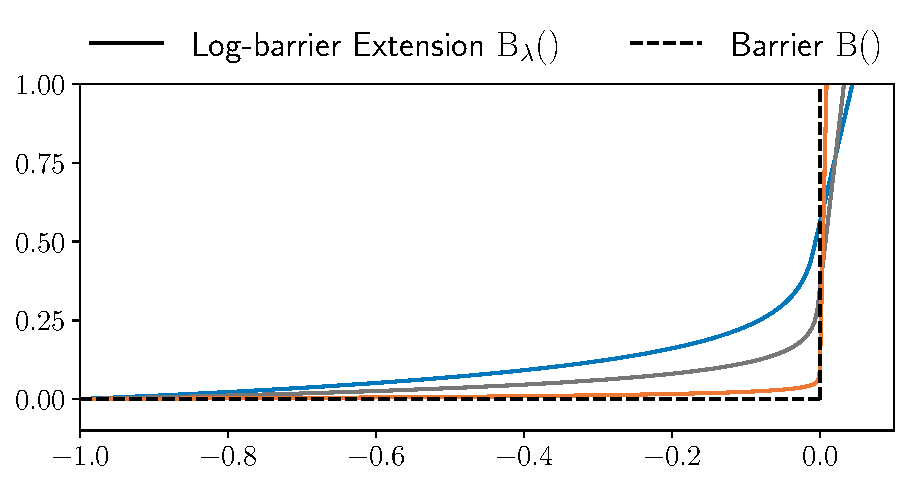
\includegraphics[width=0.8\linewidth]{chapter_4/figures/log_barrier.pdf}
    \caption[]{
    Plot of the barrier function $\logbar()$ (with the dotted line) and the log-barrier extension $\logbar_{\lambda}()$ (plain lines).
    We plot the function with three parameters: $\lambda \in \{10, 20, 100\}$.
    The higher the parameter $\lambda$, the closer the function $\logbar_{\lambda}()$ to the barrier function $\logbar()$. 
    Thus, the blue, gray and orange curves are respectively with the parameter $\lambda=10$, $\lambda=20$ and $\lambda=100$.
    }
    \label{chap:mv:fig:log_barrier}
\end{figure}

\looseness=-1
The parameter $\lambda\in\R_{*}^{+}$ parameterized the log-barrier extension $\logbar_{\lambda}()$.
The function $\logbar_{\lambda}()$ tends to $\logbar()$ when $\lambda$ tends to $+\infty$; we plot in \Cref{chap:mv:fig:log_barrier} these two functions.
Compared to the standard log-barrier\footnote{The reader can refer to \citet{BoydVandenberghe2014} for an introduction of standard log-barrier and interior-point methods.}, the function $\logbar_{\lambda}()$ is differentiable even when the constraint is not satisfied, \ie, when $a > 0$.
Thanks to $\logbar_{\lambda}()$, we can take the constraint $r_{\dS}(\Q){+}{\scriptstyle\sqrt{\frac{1}{2\m}[ \KL(\Q\|\P){+}\ln{\scriptscriptstyle\frac{4\sqrt{\m}}{\delta}}]}}\le\!\tfrac{1}{2}$ into account.
Moreover, when the number of examples $\m$ is large, we estimate the PAC-Bayesian C-Bound $\MCBound$ and the Gibbs risk $r_{\dS}(\Q)$ with a mini-batch $\batch\subseteq\S$.
Concretely, our objective function that is minimized by stochastic gradient descent with \Cref{chap:mv:algo:mcallester} is the following:
\begin{align*}
   \MObjbatch \ =\ \MCBoundbatch + \logbar_{\lambda}\LB r_{\dbatch}(\Q){+}\sqrt{\frac{1}{2\m}\LB \KL(\Q\|\P){+}\ln\frac{4\sqrt{\m}}{\delta}\RB}{-}\frac{1}{2}\RB.
\end{align*}
For a given $\lambda$, the optimizer will find a solution with a good trade-off between minimizing $\MCBoundbatch$ and the log-barrier extension function $\logbar_{\lambda}()$.
As shown in the experiments, minimizing the \citeauthor{McAllester2003}-based bound does not lead to the tightest bound.
Indeed, such a bound is looser than \citeauthor{Seeger2002}-based bounds and leads to a looser PAC-Bayesian C-Bound. 
\subsection{Algorithm based on \Cref{chap:mv:eq:cbound-seeger}}

In order to obtain better generalization guarantees, we should optimize the \citeauthor{Seeger2002}-based C-bound of \Cref{chap:mv:theorem:cbound-seeger}. 
Hence to minimize such a PAC-Bayesian C-Bound, we seek to minimize the following optimization problem:
\begin{align*}
    \min_{\Q\in\M(\H)}& \underbrace{\LC 1{-}\frac{\LP1{-}2\min\LB\frac{1}{2},  \klmax \LP r_{\dS}(\Q) \;\middle|\; \frac{1}{\m}\LB \KL(\Q\|\P){+}\ln\tfrac{4\sqrt{\m}}{\delta}\RB\RP\RB\RP^2}{1{-}2\max\LB 0,
\klmin\LP d_{\dS}(\Q) \;\middle|\; \frac{1}{\m}\LB 2\KL(\Q\|\P){+}\ln\tfrac{4\sqrt{\m}}{\delta}\RB\RP\RB}\RC}_{\displaystyle \defeq\ \SCBound}\\
&\text{s.t }\quad \klmax \LP r_{\dS}(\Q) \;\middle|\; \tfrac{1}{\m}\!\LB \KL(\Q\|\P){+}\ln\tfrac{4\sqrt{\m}}{\delta}\RB\RP\le\frac{1}{2}.
\end{align*}
For the same reasons as for deriving \Cref{chap:mv:algo:mcallester}, we propose to solve by stochastic gradient descent with a mini-batch $\batch\subseteq\S$:
\begin{align*}
\SObjbatch = \SCBoundbatch + \logbar_{\lambda}\LB\klmax \LP r_{\dbatch}(\Q) \;\middle|\; \tfrac{1}{\m}\!\LB \KL(\Q\|\P){+}\ln\tfrac{4\sqrt{\m}}{\delta}\RB\RP-\frac{1}{2}\RB.
\end{align*}
The main challenge in optimizing it is to evaluate $\klmax$ or $\klmin$ and to compute their derivatives.
The evaluation of $\klmax$ or $\klmin$ is done by \Cref{chap:pac-bayes:algo:kl} proposed by~\citet{ReebDoerrGerwinnRakitsch2018}.
This method consists in refining iteratively an interval $[p_{\text{min}}, p_{\text{max}}]$ with \mbox{$p\in [p_{\text{min}}, p_{\text{max}}]$} such that \mbox{$\kl(q\|p)\!=\!\psi$}.
Moreover, to compute the derivatives with respect to the posterior $\Q$, we use the chain rule for differentiation with a deep learning framework (such as \pytorch~\citep{Paszke2019}) and the derivatives in \Cref{chap:pac-bayes:eq:deriv-kl}. 
The global algorithm is summarized in \Cref{chap:mv:algo:seeger}.

\subsection{Algorithm based on \Cref{chap:mv:theorem:cbound-lacasse}}

\label{section:contribution-e-d}
\Cref{chap:mv:theorem:cbound-lacasse} jointly upper-bounds the joint error $e_{\D}(\Q)$ and the disagreement $d_{\D}(\Q)$; But as pointed out in \Cref{chap:mv:section:pac-bayesian-e-d} its optimization can be hard.
To ease its manipulation, we derive below a C-Bound resulting of a reformulation of the constraints involved in the set $\Abb_{\dS}(\Q)$.

\begin{algorithm}[H]
 \caption{Minimization of \Cref{chap:mv:eq:cbound-seeger} by Stochastic Gradient Descent}
  \begin{algorithmic}
  \State{{\bf Given: } learning sample $\S$,  prior distribution $\P\in\M^{*}(\H)$, the objective function $\SObj$}
    \State{{\bf Hyperparameters: } 
    number of iterations $\iter$}
    \State{$\Q \leftarrow \P$}
    \For{$\t\leftarrow 1$ to $\iter$}
        \For{{\bf all} mini-batches $\batch\subseteq\S$}
            \State{Compute $\SObjbatch$ using \Cref{chap:pac-bayes:algo:kl}}
            \State{$\Q\leftarrow$ Update $\Q$ with $\SObjbatch$ by gradient descent}
        \EndFor
    \EndFor
    \State{\Return{$\Q$}}
  \end{algorithmic}
  \label{chap:mv:algo:seeger}
\end{algorithm}

\begin{restatable}[Reformulation of \citeauthor{LacasseLavioletteMarchandGermainUsunier2006}'s PAC-Bayesian C-Bound]{theorem}{theoremnewcboundlacasse}
For any distribution $\D$ on $\X\times\Y$, for any hypothesis set $\H$, for any distribution $\P\in\M^{*}(\H)$, for any $\delta\in(0,1]$, with probability at least $1-\delta$ over the random choice of $\S\sim\D^\m$ we have for all $\Q\in\M(\H)$
\begin{align}
    &\Risk_{\D}(\MVQ) \le \sup_{(e, d)\in \Abb'_{\dS}(\Q)} \LB 1- \frac{\LP 1-(2e+d)\RP^2}{1-2d} \RB,\label{chap:mv:eq:new-cbound-lacasse}\\ 
    \Abb'_{\dS}(\Q) = \Bigg\{ (e, d) \;\Big|\; &\kl\LP e_{\dS}(\Q),  d_{\dS}(\Q)\|e, d\RP \le \frac{1}{\m}\LB 2\KL(\Q\|\P) + \ln\tfrac{2\sqrt{\m}+\m}{\delta}\RB,\nonumber\\
&d\le 2\sqrt{\min\LP e, \tfrac{1}{4}\RP}{-}2e,\  d<\tfrac{1}{2}\Bigg\}\nonumber.
   \end{align}
\label{chap:mv:theorem:new-cbound-lacasse}
\end{restatable}
\begin{noaddcontents}\begin{proof}
Deferred to~\Cref{ap:mv:sec:proof-new-cbound-lacasse}.
\end{proof}\end{noaddcontents}

\Cref{chap:mv:theorem:new-cbound-lacasse} suggests then the following constrained optimization problem: 
\begin{align*}
    &\min_{\Q\in\M(\H)}\!\left\{\! \sup_{\scalebox{0.8}{$(e{,}d){\in}\!\LB0,\!\tfrac{1}{2}\RB^2$}}\!\!
    \LP 1\!-\! \frac{\big[ 1\!-\!(2e\!+\!d)\big]^2}{1\!-\!2d}\! \RP\,   \text{s.t.}\,  (e, d)\! \in\! \Abb'_{\dS}(\Q) \! \right\} \!\text{ s.t. } 2e_{\dS}(\Q){+}d_{\dS}(\Q)\!\le\! 1,
\end{align*}
Actually, we can rewrite this constrained optimization problem into an unconstrained one using the barrier function. 
We obtain
\begin{align}
    \min_{\Q\in\M(\H)} \Bigg\{&\max_{\scalebox{0.8}{$(e{,}d){\in}\!\LB0,\!\tfrac{1}{2}\RB^2$}}  \Bigg(
     \CBound^{\tt L}(e,d) - \logbar\!\LB d {-} 2\sqrt{\min\LP e, \tfrac{1}{4}\RP}{-}2e\RB -\logbar\!\LB d{-}\tfrac{1}{2}\RB \nonumber\\
     &- \logbar\LB\kl\LP e_{\dS}(\Q),  d_{\dS}(\Q)\|e, d\RP{-}\frac{1}{\m}\LB 2\KL(\Q\|\P) + \ln\tfrac{2\sqrt{\m}+\m}{\delta}\RB\RB
   \Bigg)\nonumber\\
   &+ \logbar\Big[ 2e_{\dS}(\Q){+}d_{\dS}(\Q){-}1\Big]\Bigg\}, \label{eq:k_Q_param_nu}
\end{align}
where $\CBound^{\tt L}(e,d)=1-\tfrac{\LP 1-(2e+d)\RP^2}{1-2d}$ if $d\!<\!\frac12$, and $\CBound^{\tt L}(e,d)\!=\!1$ otherwise.
However, this problem cannot be optimized directly by stochastic gradient descent.
In this case, we have a \mbox{min-max} optimization problem, \ie, for each descent step we need to find the couple $(e, d)$ that maximizes the $\CBound^{\tt L}(e,d)$ given the three constraints that define $\Abb'_{\dS}(\Q)$ before updating the posterior distribution $\Q$.

First, to derive our optimization procedure, we focus on the inner maximization problem when $e_{\dS}(\Q)$ and $d_{\dS}(\Q)$ are fixed in order to find the optimal $(e,d)$.
However, the function $\CBound^{\tt L}(e,d)$ we aim at maximizing is not concave for all $(e,d)\!\in\!\R^2$, implying that the  implementation of its maximization can be hard\footnote{For example, when using \cvxpy~\citep{DiamondBoyd2016}, that uses Disciplined Convex Programming (DCP~\citep{GrantBoydYe2006}), the maximization of a non-concave function is not possible.}. 
Fortunately, $\CBound^{\tt L}(e,d)$ is quasi-concave~\citep{GermainLacasseLavioletteMarchandRoy2015} for $(e, d)\in[0, 1]\times[0, \frac{1}{2}]$.
Then by  definition of quasi-concavity, we have:
\begin{align*}
&\forall \alpha\in [0,1],\quad \left\{ (e, d) \,\middle|\, 1- \frac{\big[ 1-(2e+d)\big]^2}{1-2d} \ge 1-\alpha \right\}\\
\Longleftrightarrow\quad  &\forall \alpha\in [0,1],\quad  \left\{ (e, d) \ \middle|\  
\alpha(1{-}2d)-\Big[1{-}(2e{+}d)\Big]^2 \ge 0\right\}.
\end{align*}

\begin{algorithm}[t]
  \caption{Minimization of \Cref{chap:mv:eq:new-cbound-lacasse} by Stochastic Gradient Descent}
  \begin{algorithmic}
    \State{{\bf Given: } learning sample $\S$, prior $\P\in\M^{*}(\H)$, the objective function $\LObj$}
    \State{{\bf Hyperparameters: }
    number of iterations $\iter$}
    \State{$\Q \leftarrow \P$}
    \For{$\t\leftarrow 1$ to $\iter$}
        \For{{\bf all} mini-batches $\batch\subseteq\S$}
        \State{$(e^*, d^*) \leftarrow $\Call{maximize-$e$-$d$}{$e_{\dbatch}(\Q), d_{\dbatch}(\Q)$}}
        \State{$\Q\leftarrow$ Update $\Q$ with $\LObjbatch$ by gradient descent}
        \EndFor
    \EndFor
    \State{\Return{$\Q$}}\\
    {\centerline{\rule{0.75\linewidth}{0.25pt}}}
      \State{{\bf Given:} learning sample $\S$, joint error $e_{\dS}(\Q)$, disagreement $d_{\dS}(\Q)$}
\State{{\bf Hyperparameters: }tolerance $\epsilon$}
\Function{maximize-$e$-$d$}{$e_{\dS}(\Q), d_{\dS}(\Q)$}
\State{$\alpha_{\text{min}} = 0$ and $\alpha_{\text{max}}=1$}
\While{$\alpha_{\text{max}}-\alpha_{\text{min}}>\epsilon$}
\State{$\alpha=\tfrac{1}{2}(\alpha_{\text{min}}+\alpha_{\text{max}})$}
\State{$(e, d) \leftarrow$ Solve \Cref{chap:mv:eq:min-e-d}}
\State{\textbf{if} $\CBound^{\tt L}(e,d) \ge 1{-}\alpha$ \textbf{then} $\alpha_{\text{max}} \leftarrow \alpha$ \textbf{else} $\alpha_{\text{min}} \leftarrow \alpha$}
\EndWhile
\State{\Return{$(e, d)$}}
\EndFunction
\end{algorithmic}
\label{chap:mv:algo:lacasse}
\end{algorithm}
\noindent Hence, for any fixed $\alpha\!\in\![0, 1]$ we can look for $(e, d)$ that maximizes $\CBound^{\tt L}(e,d)$ and respects the constraints involved in $\Abb'_{\dS}(\Q)$.
This is equivalent to solving the following problem for a given $\alpha\in[0, 1]$:
\begin{align}
    \max_{(e, d)\in[0, \frac{1}{2}]^2}\quad  &\alpha(1{-}2d)-\Big[1{-}(2e{+}d)\Big]^2\label{chap:mv:eq:min-e-d}\\
    \text{ s.t. } d&\le 2\sqrt{\min\LP e, \tfrac{1}{4}\RP}{-}2e\nonumber\\
    \text{ and }\kl\big( e_{\dS}(\Q),  d_{\dS}(\Q)\|e, d&\big)\le \frac{1}{\m}\LB 2\KL(\Q\|\P) + \ln\tfrac{2\sqrt{\m}+\m}{\delta}\RB\nonumber.
\end{align}
In fact, we aim at finding $\alpha\in[0,1]$ such that the maximization of \Cref{chap:mv:eq:min-e-d} leads to $1{-}\alpha$ equals to the largest value of $C^{\tt L}(e, d)$ under the constraints.
To do so, we make use of the ``Bisection method for quasi-convex optimization''~\citep{BoydVandenberghe2014} that is summarized in  \textsc{maximize-$e$-$d$} in \Cref{chap:mv:algo:lacasse}.
We denote by $(e^{*\!}, d^*)$ the solution of \Cref{chap:mv:eq:min-e-d}.
Note that, in practice, the joint error and the disagreement is approximated through the mini-batch $\batch\subseteq\S$.
It remains then to solve the outer minimization problem that becomes:
\begin{align*}
    \min_{\Q\in\M(\H)}\Bigg\{\ &\logbar\LB 2e_{\dS}(\Q){+}d_{\dS}(\Q){-}1\RB\\
    &-\logbar\LB\kl\LP e_{\dS}(\Q),  d_{\dS}(\Q)\|e^{*\!}, d^*\RP{-}\frac{1}{\m}\LB 2\KL(\Q\|\P) + \ln\tfrac{2\sqrt{\m}+\m}{\delta}\RB\RB\ \Bigg\}.
\end{align*}
To obtain a objective function that is suitable for stochastic gradient descent, we bring two modifications to the outer minimization problem: {\it (i)} we replace $\logbar()$ by the log-barrier extension $\logbar_\lambda()$ and {\it (ii)} we approximate the disagreement and the joint error with a mini-batch $\batch\subseteq\S$.
Hence, we obtain the following objective function: 
\begin{align*}
   \LObjbatch = & \logbar_{\lambda}\LB 2e_{\dbatch}(\Q){+}d_{\dbatch}(\Q){-}1\RB
   \\
    &\hspace{-1cm}-\logbar_\lambda \LB\kl\LP e_{\dbatch}(\Q),d_{\dbatch}(\Q)\|e^{*\!},d^*\RP{-}\frac{1}{\m}\LB 2\KL(\Q\|\P) + \ln\tfrac{2\sqrt{\m}+\m}{\delta}\RB\RB.
\end{align*}
The global method is summarized in \Cref{chap:mv:algo:lacasse}.
\noindent As a side note, we  mention that the classic Danskin Theorem~\citep{Danskin1966} used in min-max optimization theory is not applicable in our case since our objective function is not differentiable for all $(e, d)\in[0, \tfrac{1}{2}]^2$. 
We discuss this point in \Cref{ap:mv:sec:danskin}.

\section{Experiments}
\label{chap:mv:sec:expe}

\subsection{Setting}

\begin{figure}
    \centering
    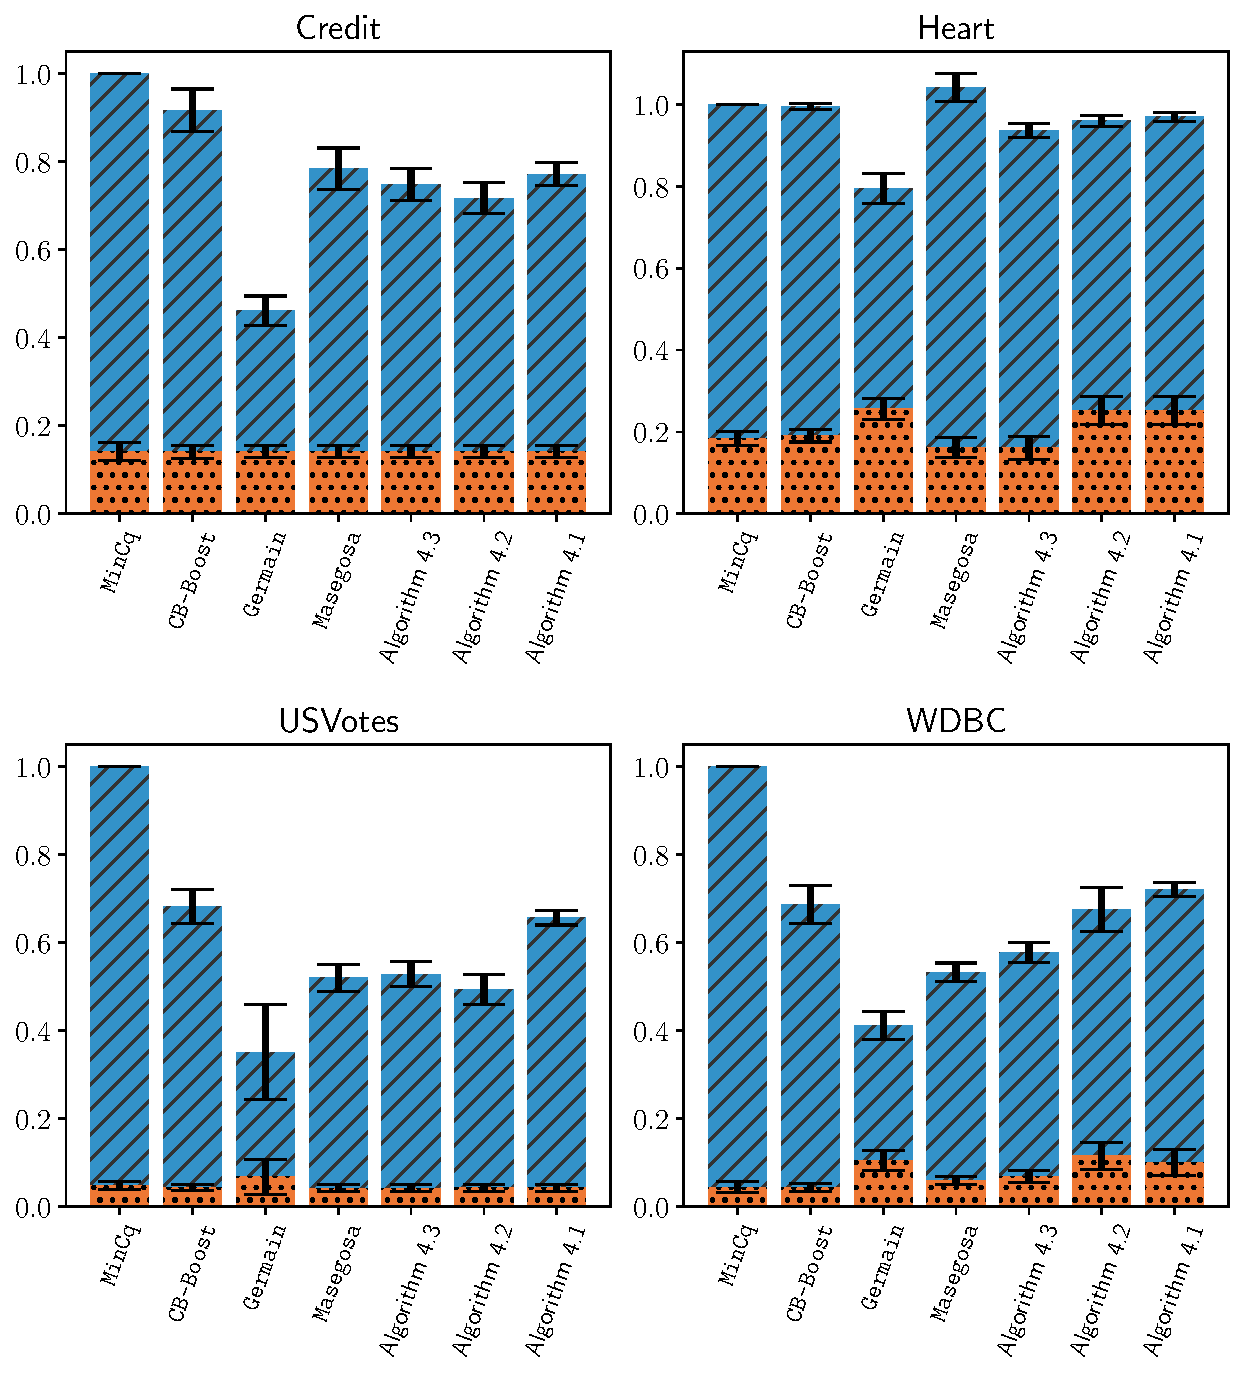
\includegraphics[width=1.0\linewidth]{chapter_4/figures/stump_binary_1.pdf}
    \caption[Comparison Between the Test Risks and the Bounds (1/6)]{
    Plot of a comparison between the test risks $\Risk_{\dT}(\MVQ)$ and the generalization bounds in the binary setting when the voters are decision stumps.
    For each algorithm, we represent the mean of the test risks in the orange bars and the bounds' mean in the blue bars.
    Additionally, the black lines are the standard deviations. 
    }
    \label{chap:mv:fig:stump-binary-1}
\end{figure}

\begin{figure}
    \centering
    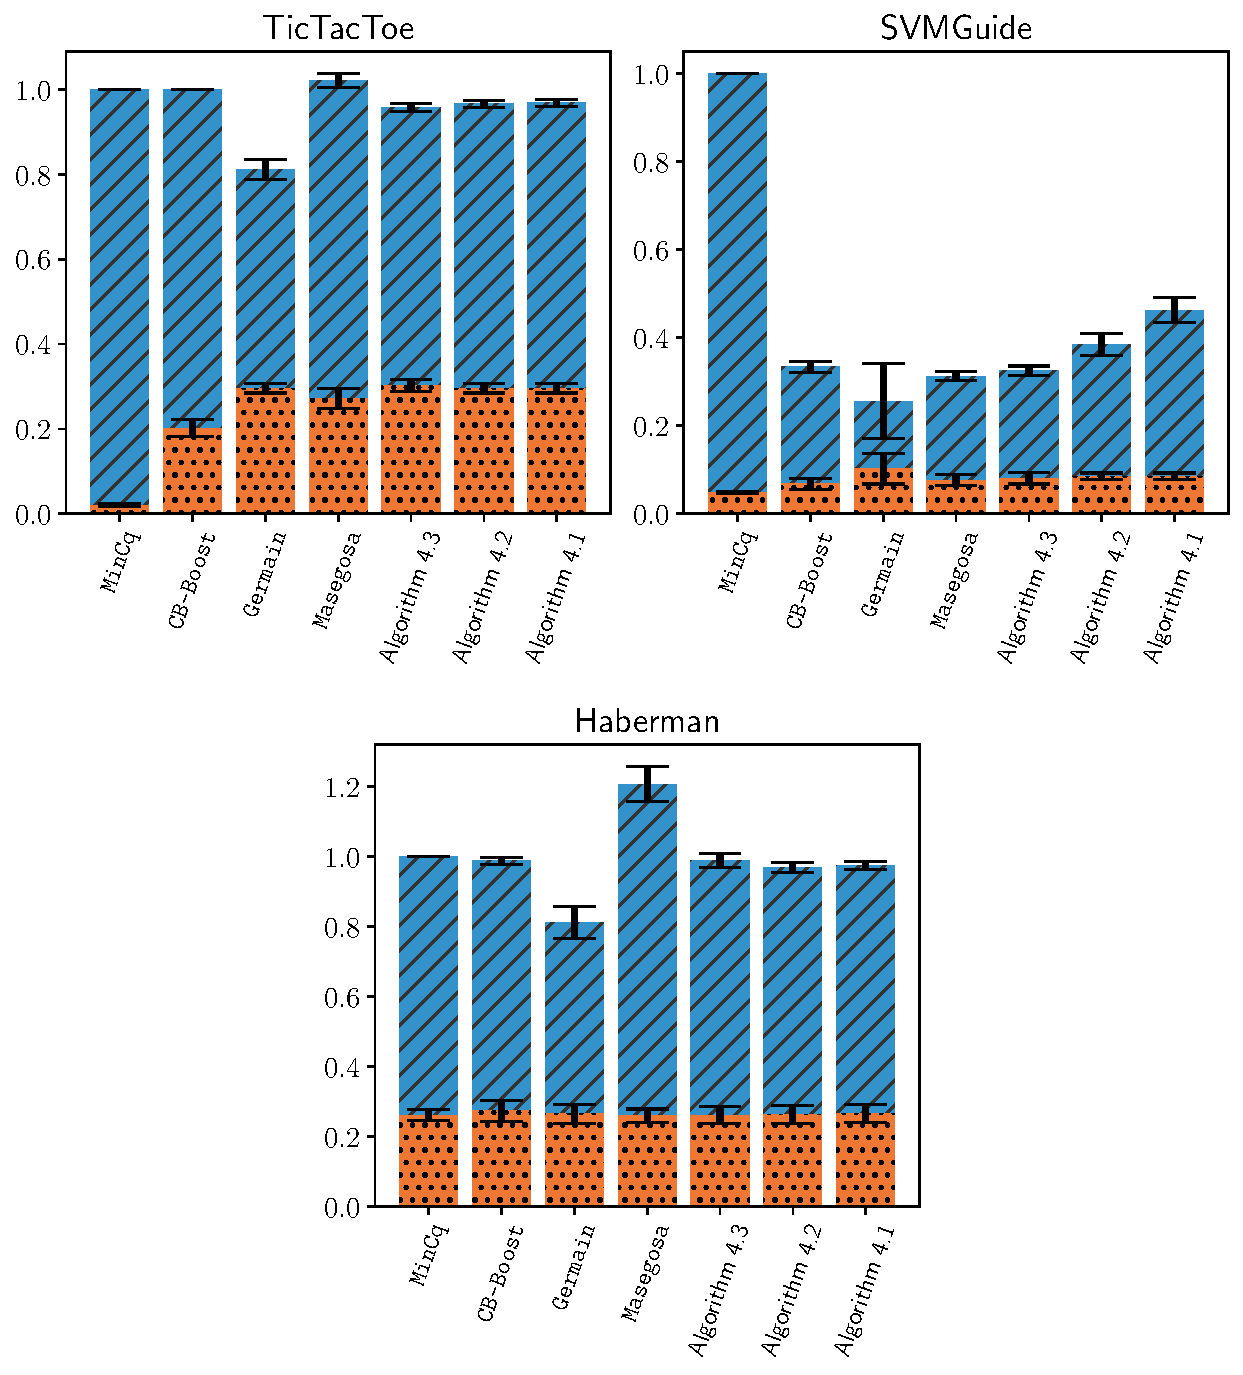
\includegraphics[width=1.0\linewidth]{chapter_4/figures/stump_binary_2.pdf}
    \caption[Comparison Between the Test Risks and the Bounds (2/6)]{
    Plot of a comparison between the test risks $\Risk_{\dT}(\MVQ)$ and the generalization bounds in the binary setting when the voters are decision stumps.
    For each algorithm, we represent the mean of the test risks in the orange bars and the bounds' mean in the blue bars.
    Additionally, the black lines are the standard deviations. 
    }
    \label{chap:mv:fig:stump-binary-2}
\end{figure}

\begin{figure}
    \centering
    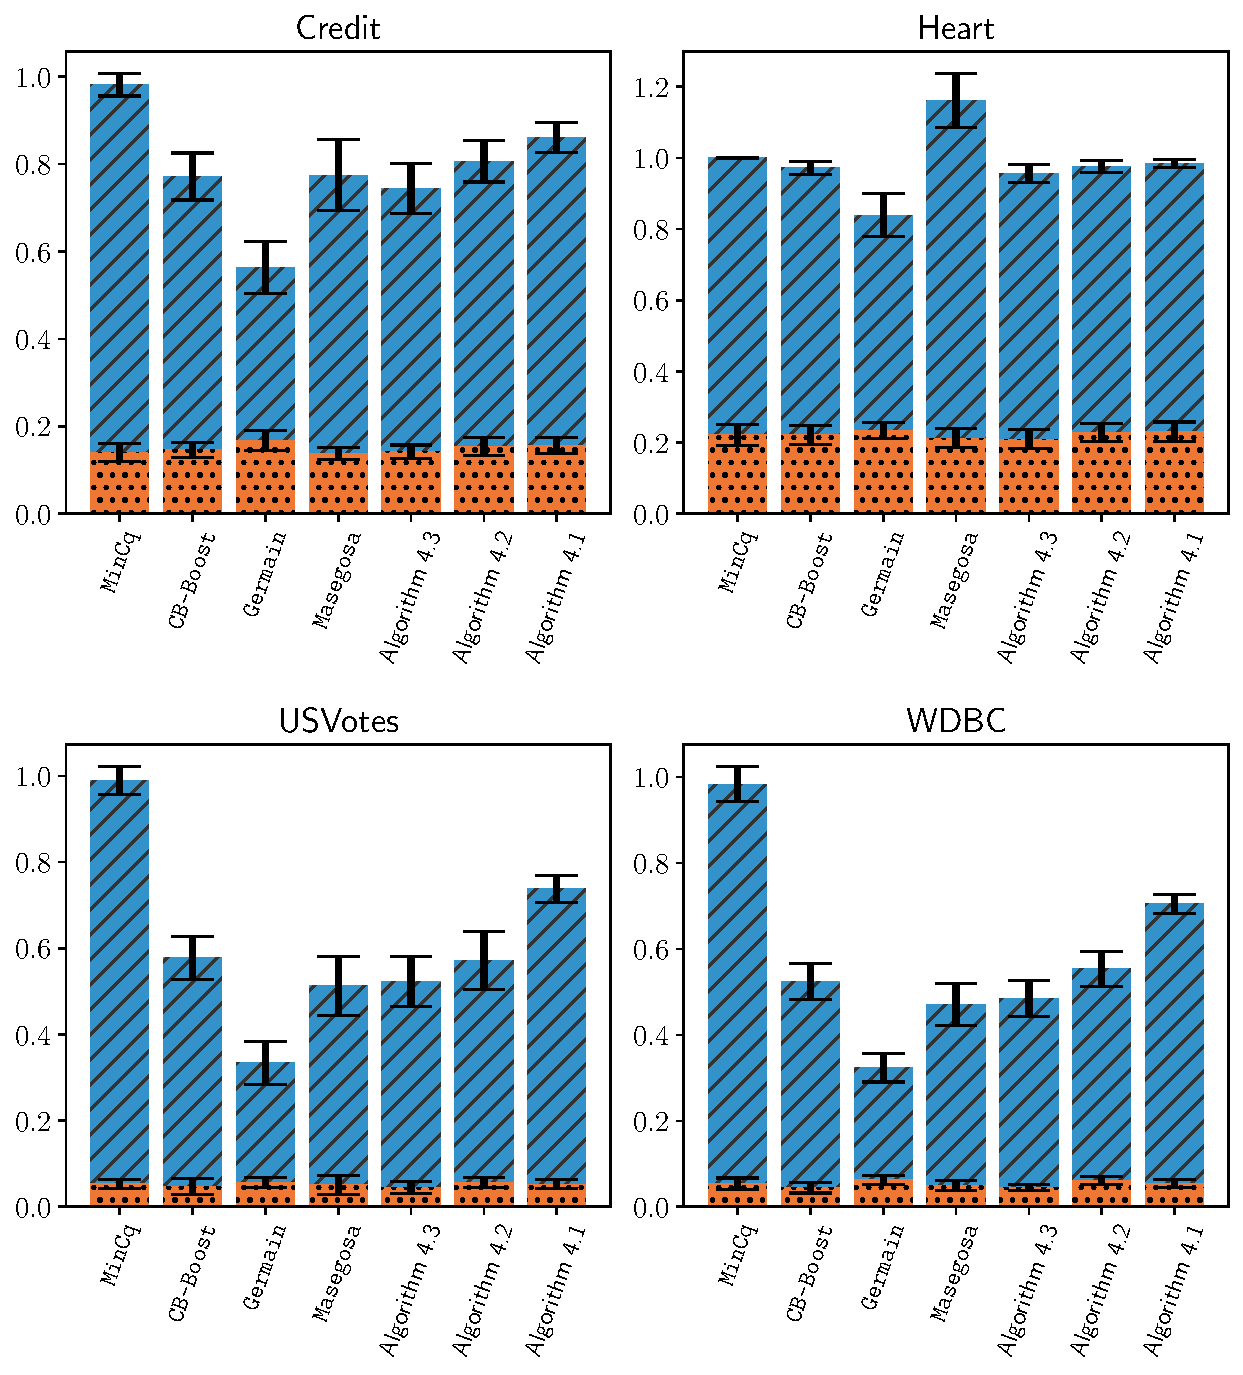
\includegraphics[width=1.0\linewidth]{chapter_4/figures/tree_binary_1.pdf}
    \caption[Comparison Between the Test Risks and the Bounds (3/6)]{
    Plot of a comparison between the test risks $\Risk_{\dT}(\MVQ)$ and the generalization bounds in the binary setting when the voters are decision trees.
    For each algorithm, we represent the mean of the test risks in the orange bars and the bounds' mean in the blue bars.
    Additionally, the black lines are the standard deviations. 
    }
    \label{chap:mv:fig:tree-binary-1}
\end{figure}

\begin{figure}
    \centering
    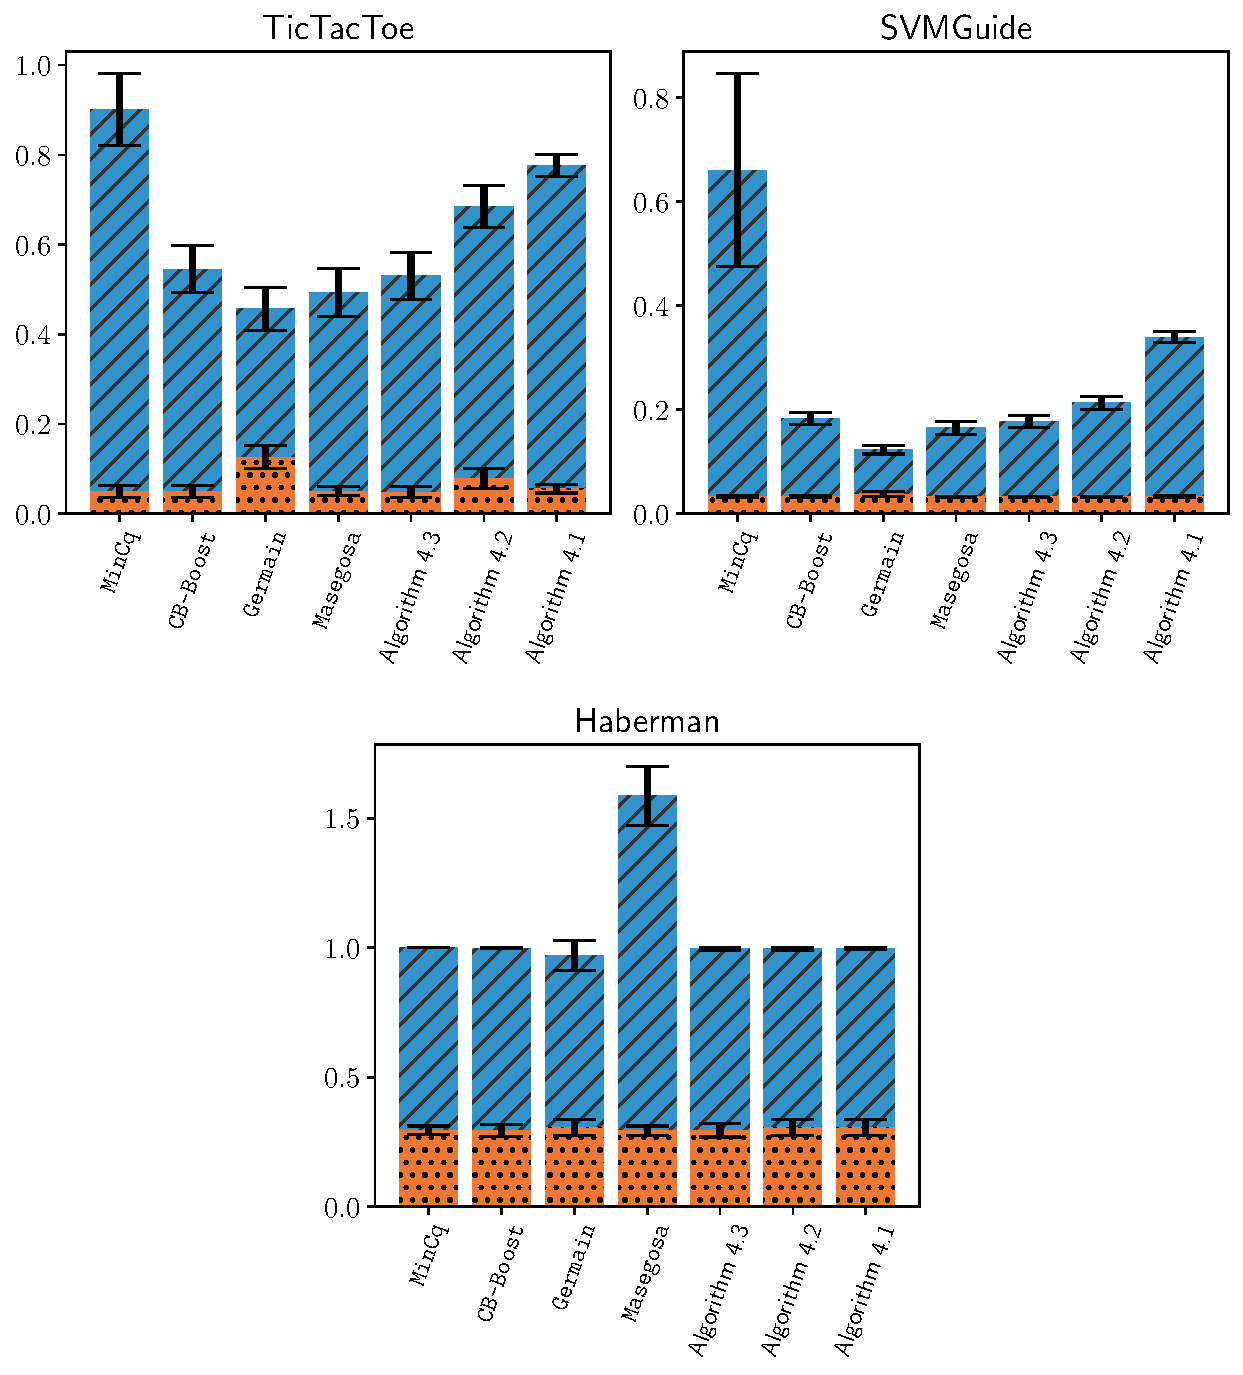
\includegraphics[width=1.0\linewidth]{chapter_4/figures/tree_binary_2.pdf}
    \caption[Comparison Between the Test Risks and the Bounds (4/6)]{
    Plot of a comparison between the test risks $\Risk_{\dT}(\MVQ)$ and the generalization bounds in the binary setting when the voters are decision trees.
    For each algorithm, we represent the mean of the test risks in the orange bars and the bounds' mean in the blue bars.
    Additionally, the black lines are the standard deviations. 
    }
    \label{chap:mv:fig:tree-binary-2}
\end{figure}

\begin{figure}
    \centering
    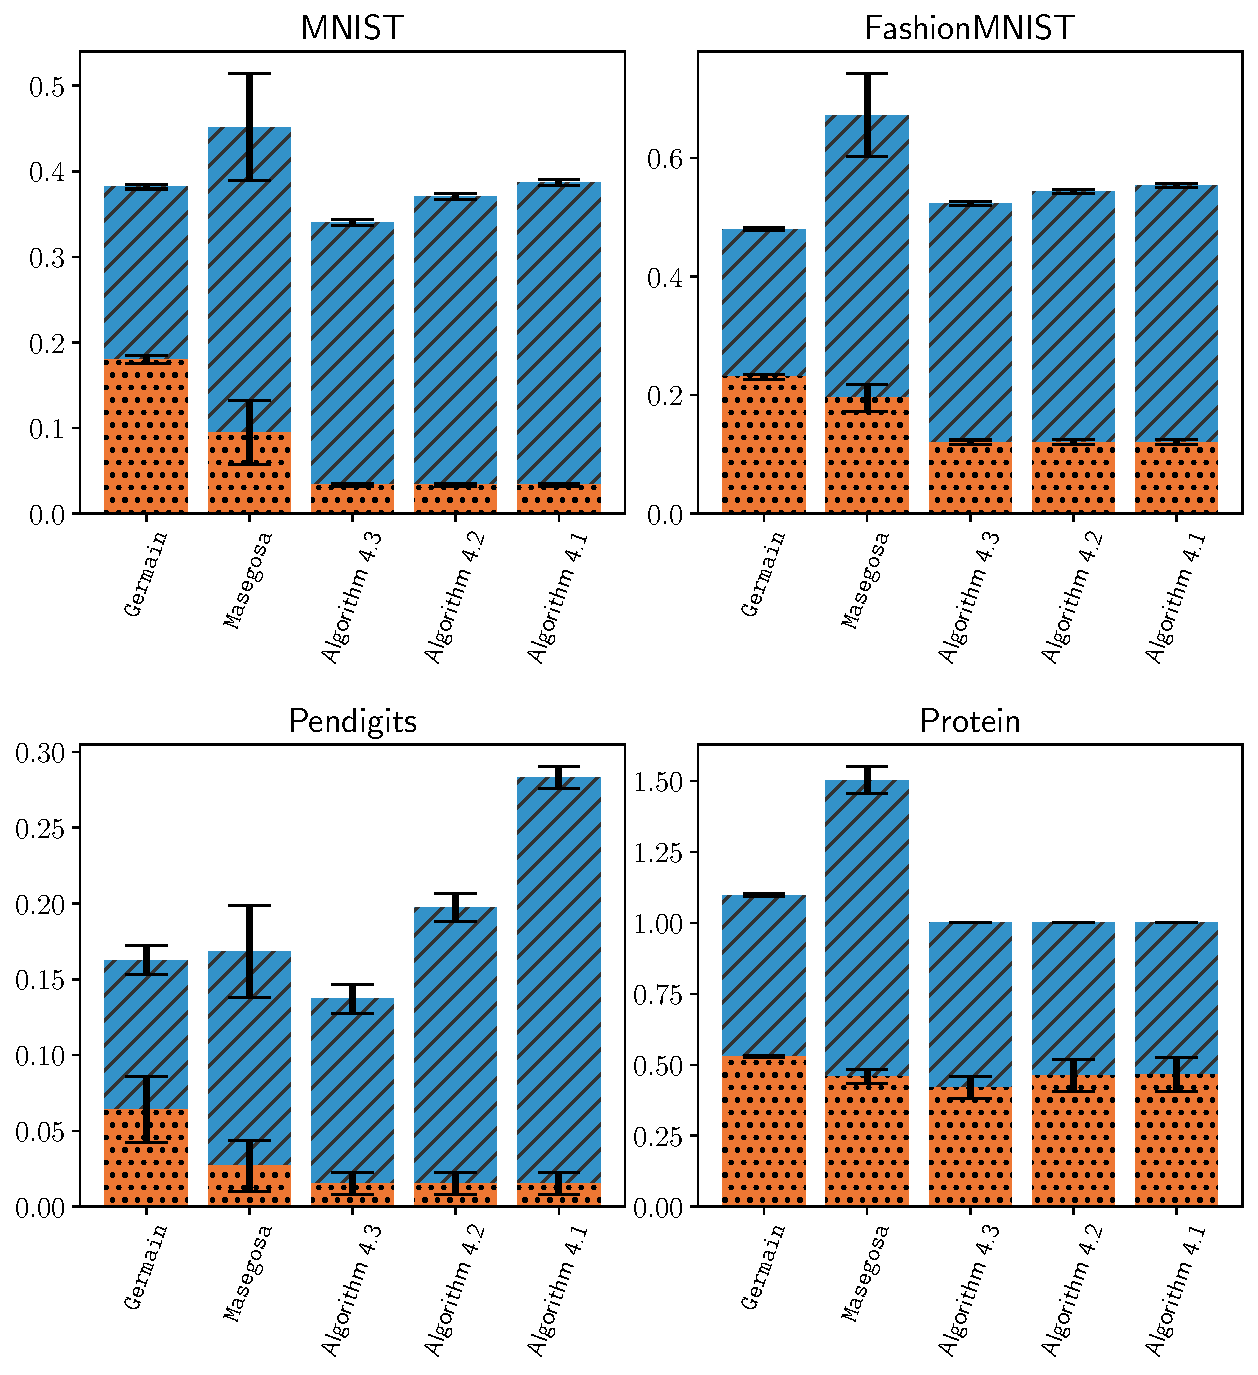
\includegraphics[width=1.0\linewidth]{chapter_4/figures/tree_multi_1.pdf}
    \caption[Comparison Between the Test Risks and the Bounds (5/6)]{
    Plot of a comparison between the test risks $\Risk_{\dT}(\MVQ)$ and the generalization bounds in the multi-class setting when the voters are decision trees.
    For each algorithm, we represent the mean of the test risks in the orange bars and the bounds' mean in the blue bars.
    Additionally, the black lines are the standard deviations. 
    }
    \label{chap:mv:fig:tree-multi-1}
\end{figure}

\begin{figure}
    \centering
    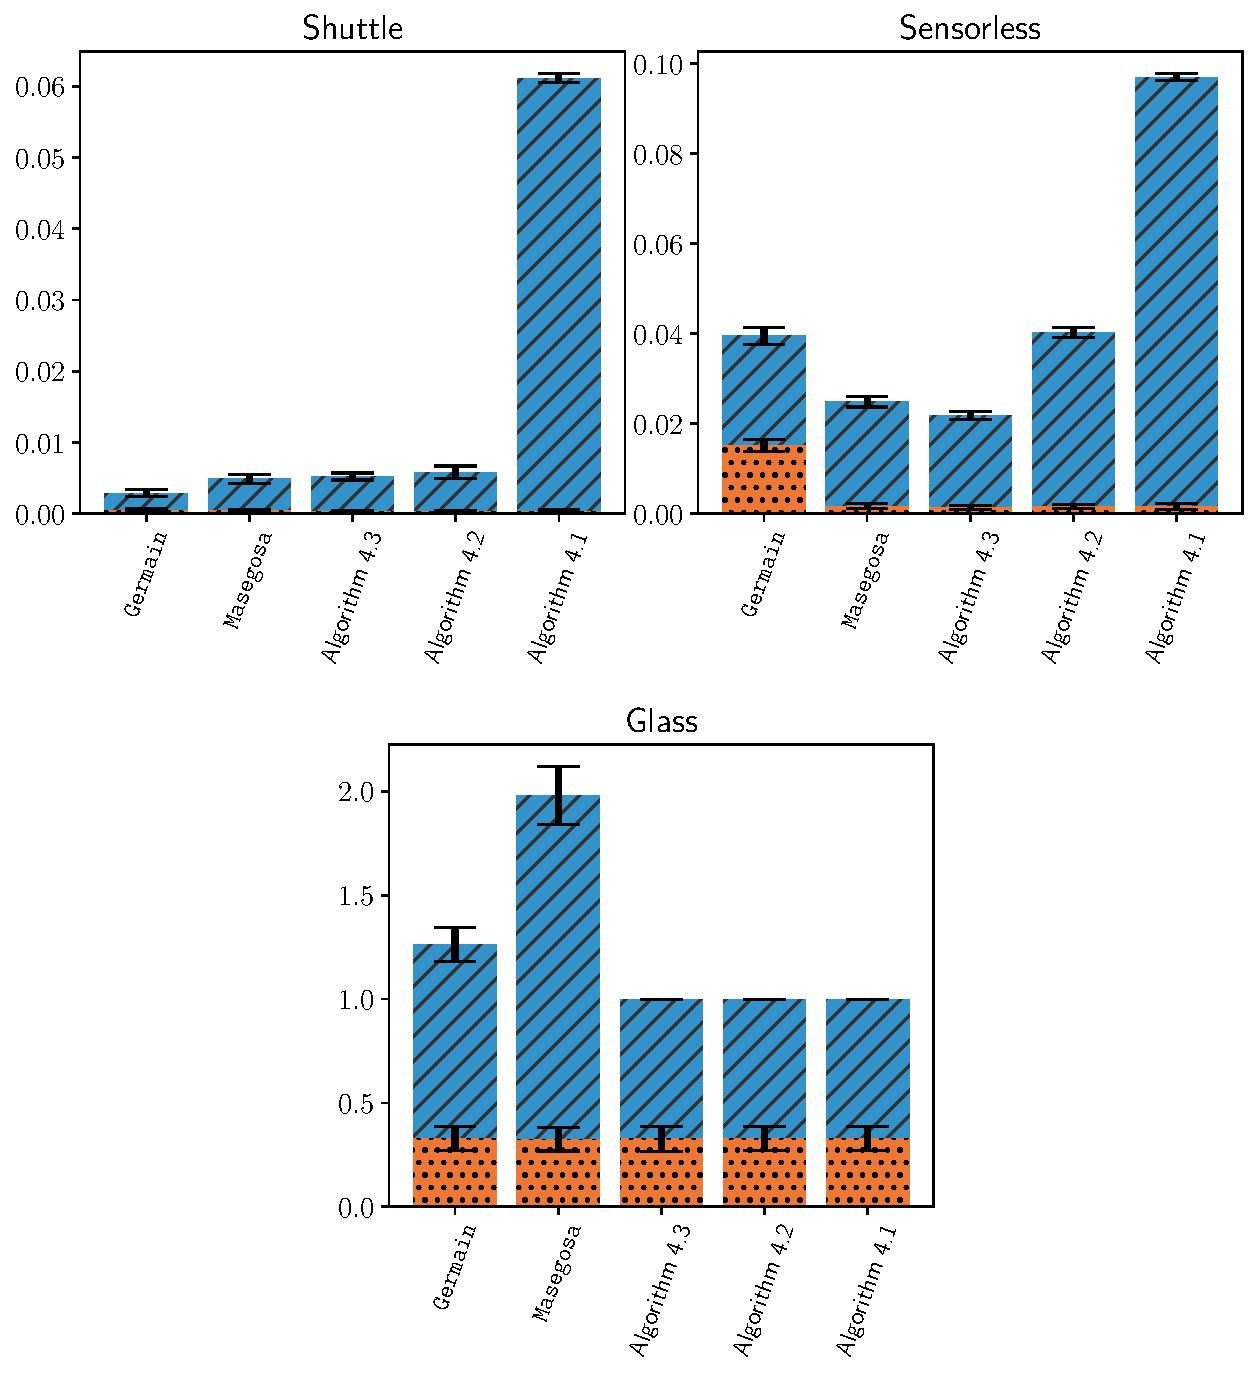
\includegraphics[width=1.0\linewidth]{chapter_4/figures/tree_multi_2.pdf}
    \caption[Comparison Between the Test Risks and the Bounds (6/6)]{
    Plot of a comparison between the test risks $\Risk_{\dT}(\MVQ)$ and the generalization bounds in the multi-class setting when the voters are decision trees.
    For each algorithm, we represent the mean of the test risks in the orange bars and the bounds' mean in the blue bars.
    Additionally, the black lines are the standard deviations. 
    }
    \label{chap:mv:fig:tree-multi-2}
\end{figure}

Our experiments have a two-fold objective: \textit{(i)} assessing the guarantees given by the associated PAC-Bayesian bounds, and \textit{(ii)} comparing the performance of the different C-bound-based algorithms in terms of risk optimization.
We introduce the setting in the following and we report in \Cref{chap:mv:fig:stump-binary-1,chap:mv:fig:stump-binary-2,chap:mv:fig:tree-binary-1,chap:mv:fig:tree-binary-2,chap:mv:fig:tree-multi-1,chap:mv:fig:tree-multi-2} the mean/standard deviation of the risks on the test set $\T$ and the bound values (with $\delta=0.05$) for 10 runs; see also \Cref{ap:mv:sec:details} for more details.
The setting of the experiments is as follows.

\paragraph{Dataset.}
We consider several binary and multi-class datasets like FashionMNIST \citep{XiaoRasulVollgraf2017}, MNIST~\citep{LeCunCortesBurges1998} and some coming from the UCI repository~\citep{DuaGraff2017}.
For each different run, we keep the same number of examples in the test or the train set as in the original split.
When there is no original split, we use 50\% of data in the training set $\S$ and 50\% in the test set (except for Sensorless where we have 15\% in the test set because the original set is large).

\paragraph{Voters.}
In the binary setting, we consider either a set $\H$ of decision trees or decision stumps that is complemented: if $\h\in\H$ then there is $\h'\in\H$ \st $\h'(\x)=-\h(\x)$ for all $\x\in\X$.
Concerning the multi-class setting, we only consider decision trees.
Indeed, having decision stumps would have resulted in too many voters.  
Following \citet{MasegosaLorenzenIgelSeldin2020}, the prior distribution $\P\in\M^{*}(\H)$ is set as the uniform distribution.
For the decision stumps, following \citet{RoyLavioletteMarchand2011,BauvinCapponiRoyLaviolette2020}, we use 10 decision stumps per feature.
For the decision trees, we follow a general setting similar to the one of~\citep{MasegosaLorenzenIgelSeldin2020}.
Moreover, $100$ trees are learned with $50\%$ of the training data (the remaining part serves to learn the posterior $\Q$).
More precisely, for each tree $\sqrt{d}$ features of the $d$-dimensional input space are selected, and the trees are learned by using the Gini criterion until the leaves are pure. 

\paragraph{Algorithms' parameters.}
To update of the posterior $\Q$ in \Cref{chap:mv:algo:mcallester,chap:mv:algo:seeger,chap:mv:algo:lacasse} is done through the COCOB-Backprop optimizer~\citep{OrabonaTommasi2017} (its parameter remains the default one).
In the binary setting, we optimize for $T=2,000$ iterations (by batch gradient descent), and in the multi-class setting, we set $20$ epochs with a batch size of $64$.
Lastly, we consider the parameter $\lambda{=}100$ for log-barrier extension $\logbar_{\lambda}()$.

\paragraph{Comparisons.}
We compare the three algorithms proposed in this chapter to the following state-of-the-art PAC-Bayesian methods for majority vote learning.
\begin{itemize}
    \item We compare with the algorithm proposed by \citet{MasegosaLorenzenIgelSeldin2020} that optimizes a PAC-Bayesian bound on $\Risk_{\D}(\MVQ) \le 4e_{\D}(\Q)$ (\Cref{chap:pac-bayes:theorem:4joint}); see Theorem~9 and Appendix~G of \citep{MasegosaLorenzenIgelSeldin2020} for a description of this algorithm that we denote by \algomasegosa.
    For \citeauthor{MasegosaLorenzenIgelSeldin2020}'s algorithm, we kept the original parameters.

    \item Our algorithm to optimize the PAC-Bayesian bound on $\Risk_{\D}(\MVQ) \le 2r_\D(\Q)$ (\Cref{chap:pac-bayes:theorem:2gibbs}) recalled in \Cref{chap:mv:theorem:pb-2gibbs} and derived by \citep[PAC-Bound 0]{GermainLacasseLavioletteMarchandRoy2015}.
    Even though \citep{GermainLacasseLavioletteMarchandRoy2015} does not optimize the bound, we denote this algorithm by \algogermain.
    The algorithm is similar to \Cref{chap:mv:algo:seeger}, but without the numerator of the C-Bound (\ie, the disagreement); more details are given in \Cref{ap:mv:sec:pb-2gibbs}.

    \item In the binary setting only, we compare with \mincq \citep{RoyLavioletteMarchand2011} and \cbboost \citep{BauvinCapponiRoyLaviolette2020} that are based on the minimization of the empirical C-Bound $\CBound_{\dS}(\Q)$.
    Indeed, these algorithms are developed for this setting only.
    For comparison purposes and since \mincq and \cbboost do not explicitly minimize a PAC-Bayesian bound, we report the bound values of \Cref{chap:mv:theorem:new-cbound-lacasse} instantiated with the models learned;
    Moreover, for \mincq, we select the margin parameter among $20$ values uniformly spaced between $[0,\tfrac{1}{2}]$ by 3-fold cross validation. 
    For \cbboost, which is based on a Boosting approach, we fix the maximal number of boosting iterations to $200$.
\end{itemize}

\subsection{Analysis of the Results}

When comparing only the PAC-Bayesian C-Bounds, we observe in \Cref{chap:mv:fig:stump-binary-1,chap:mv:fig:stump-binary-2,chap:mv:fig:tree-binary-1,chap:mv:fig:tree-binary-2,chap:mv:fig:tree-multi-1,chap:mv:fig:tree-multi-2} that \Cref{chap:mv:algo:mcallester} provides the worst bound.
\Cref{chap:mv:algo:lacasse} provides usually tighter bounds than \Cref{chap:mv:algo:mcallester,chap:mv:algo:seeger} except for Harberman and USVotes.
We believe that \Cref{chap:mv:algo:lacasse} provides lower bounds than \Cref{chap:mv:algo:seeger} because the \citeauthor{LacasseLavioletteMarchandGermainUsunier2006}'s approach bounds simultaneously the joint error and the disagreement.
\Cref{chap:mv:algo:lacasse} appears then to be the best algorithm among our three self-bounding algorithms that minimize a PAC-Bayesian C-Bound.
Moreover, \Cref{chap:mv:algo:lacasse} gives usually the lowest true risks or it is comparable to the two other algorithms.\\

Compared to the baselines, \algogermain~gives usually the lowest bounds among all the algorithms, but at the price of a large test risk.
This clearly illustrates the limitation of considering \textit{only} the Gibbs risk as an estimator of the majority vote risk: as discussed in \Cref{chap:pac-bayes:sec:surrogate}, the Gibbs risk is an unfair estimator since an increase in the diversity between the voters can have a negative impact on the Gibbs risk.\\
Second, compared to \citeauthor{MasegosaLorenzenIgelSeldin2020}'s approach, the results are comparable.
This behavior was expected since minimizing the bound of~\citet{MasegosaLorenzenIgelSeldin2020} or the PAC-Bayesian C-Bound boils down to minimize a trade-off between the risk and the disagreement.
Third, in the binary setting, compared to empirical C-bound minimization algorithms, we see that \Cref{chap:mv:algo:lacasse} outputs better results than \cbboost and \mincq for which the difference is significative, and the bounds are close to $1$ (\ie, non-informative).
Optimizing the risk bounds tends to provide better guarantees that justify that optimizing the empirical C-bound is often too optimistic (as done in \cbboost or \mincq); we provide in \Cref{ap:mv:sec:joint-disa} an illustration of the different solutions obtained from the algorithms.\\

Overall, from these experiments, our \Cref{chap:mv:algo:lacasse} is the one that provides the best trade-off between having good performances in terms of risk optimization and ensuring good theoretical guarantees with informative bounds.
Moreover, in \Cref{ap:mv:sec:time} we show that \Cref{chap:mv:algo:lacasse} has a higher computation time than the others algorithms.
This makes \Cref{chap:mv:algo:seeger} a good trade-off between ensuring good theoretical guarantees and having a low computation time.

\section{Conclusion and Summary}

This chapter presents learning algorithms that minimize the majority vote's risk with PAC-Bayesian generalization bounds based on the C-Bound. 
More precisely, we propose solving three optimization problems, each derived from an existing PAC-Bayesian bound.
Our methods belong to the class of {\it self-bounding} learning algorithms~\citep{Freund1998}: the learned predictor comes with a tight and statistically valid risk upper bound.
Our experimental evaluation has confirmed the quality of the learned predictor and the tightness of the bounds with respect to state-of-the-art methods minimizing the C-Bound.\\

As we said before, no algorithm minimizes the {\it empirical} C-Bound in the multi-class setting.
One of the reasons is that it is not easy to find a convex program like for \mincq or \pmincq algorithm.
Hopefully, thanks to the deep learning framework, minimizing the C-Bound is possible even without convexity through a stochastic gradient descent algorithm (as we show in \Cref{chap:mv-sto} in the binary setting).
Hence, in the future, we plan to explore more the minimization of the C-Bound.\\

However, one drawback of the PAC-Bayesian C-Bounds and the other ones of the literature is that the majority vote true risk is not directly minimized: we need surrogates such as the Gibbs risk, the disagreement, or the joint error.
Indeed, the C-Bound is already an upper bound on the true risk, which makes the PAC-Bayesian C-Bound even looser, thus, these generalization bounds cannot be tight.
To avoid this issue, we bound the {\it expected} true risk of the majority vote.
This is done in the next chapter: we {\it (i)} introduce the {\it stochastic} majority vote that samples a distribution $\Q$ for each prediction, and we {\it (ii)} provide guarantee on the true risk for this classifier.
As we will see, our obtained (PAC-Bayesian) guarantee is differentiable, and we can derive self-bounding learning to learn such a classifier.
%\chapter[Wasserstein PAC-Bayes Learning: Exploiting Optimisation Guarantees to Explain Generalisation]{Wasserstein PAC-Bayes Learning: Exploiting Optimisation Guarantees to Explain Generalisation}
\label{chap: wass-pb}
\addchapterlof
\addchapterloa
\addchapterloe

\vspace{-1.6cm}
\begin{center}
\textbf{This chapter is based on the following papers}\\
\end{center}
\vspace{-0.3cm}
\printpublication{haddouche2023wasserstein}
\\
\printpublication{viallard2023learning}

\vspace{-0.3cm}
\minitoc

\vspace{-0.2cm}

\begin{abstract}
    Put WPB here, precise that, when the prior is seen as the learning goal, it is possible for a certain optimisation algorithm to directly incorporate sound geometric optimisation guarantee into a generalisation bound, trading the hope to reach a flat minima with a sound convergence guarantees. However, this comes at the cost of the explicit impact of the dimension. Also put the paper with Paul(batch bounds) as a supplementary content.
\end{abstract}

\newpage

\section{Introduction}



% ----------------------------------------------------------------------------------------------- %

\part[Beyond PAC-Bayesian Bounds:\\ From Disintegration to Novel Bounds]{Beyond PAC-Bayesian Bounds:\\ {\LARGE From Disintegration to Novel Bounds}
}
\label{part:contrib-disintegrated}

%%!TEX root = main.tex
\chapter[Wasserstein PAC-Bayes in Practice: Genrealisation-Driven Learning Algorithms for Deterministic Predictors]{Wasserstein PAC-Bayes in Practice: Genrealisation-Driven Learning Algorithms for Deterministic Predictors}
\label{chap: wpb-practical}
\addchapterlof
\addchapterloe

\vspace{-2.0cm}
\begin{center}
\textbf{This chapter is based on the following paper}\\[-0.1cm]
\end{center}
TODO
%\printpublication{ViallardGermainHabrardMorvant2022}

\vspace{0.2cm}
\minitoc 

\begin{abstract}
\vspace{-0.2cm}
After \Cref{chap: wass-pb} which proposed a theoretical study of PAC-Bayes learning with Wasserstein distances, building bridges with the exploiting of convergence guarantees in generalisation, we now focus on practical expansions of Wasserstein PAC-Bayes. The optimisation view of PAC-Bayes learning is deeply exploited here: we derive theory-driven batch and online algorithms (the online paradigm attenuates the impact of the prior) valid for deterministic predictors (and thus consistent with many practical optimisation algorithms) and are derived from bounds valid for heavy-tailed lipschitz losses (weak statistical assumption and a stronger geometric one to be in line with the optimisation literature). This chapter shows that the optimisation view of PAC-Bayes leads to efficient procedures, competing with classical methods.
\end{abstract}

\newpage
    
\section{Introduction}

\Cref{chap: wass-pb} introduced Wasserstein PAC-Bayes learning from a theoretical perspective. Indeed, the main goal there was to incorporate the convergence guarantees of existing algorithms onto a generalisation bound. On the contrary, we focus here on deriving novel learning algorithms from Wasserstein PAC-Bayes bounds, circumventing many classical limitations of KL-based PAC-Bayes, which is the major part of the literature. Indeed, the practical use of KL divergence comes with two main limitations: {\it (i)} as illustrated in the generative modeling literature, the KL divergence does not incorporate the underlying geometry or topology of the data space $\Z$, hence can behave in an erratic way \cite{arjovsky2017wasserstein},
{\it (ii)} the $\KL$ divergence and its variants require the posterior $\Q$ to be absolutely continuous with respect to the prior $\P$.
However, recent studies \citep{camuto2021fractal} have shown that, in stochastic optimisation, the distribution of the iterates, which is the natural choice for the posterior, can converge to a \emph{singular distribution}, which does not admit a density with respect to the Lebesgue measure.
Moreover, the structure of the singularity (\ie, the \emph{fractal dimension} of $\Q$) depends on the data sample $\S$ \citep{camuto2021fractal}. 
Hence, in such a case, it would not be possible to find a suitable prior $\P$ that can dominate $\Q$ for almost every $\S \sim \D^m$, which will trivially make $\KL(\Q\|\P) = +\infty$ and the generalisation bound vacuous. 

Some works have focused on replacing the Kullback-Leibler divergence with more general divergences in PAC-Bayes \citep{alquier2018simpler,ohnishi2021novel,picard2022change}, although the problems arising from the presence of the $\KL$ divergence in the generalisation bounds are actually not specific to PAC-Bayes: information-theoretic bounds \citep{goyal2017pac,xu2017info,russo2020how} also suffer from similar issues as they are based on a mutual information term, which is the $\KL$ divergence between two distributions.
In this context, as a remedy to these issues introduced by the $\KL$ divergence, \cite{zhang2018optimal,wang2019information,rodriguez2021tighter,lugosi2022generalization} proved analogous bounds that are based on the \emph{Wasserstein distance}, which arises from the theory of optimal transport~\cite{monge1781memoire}.
As the Wasserstein distance inherits the underlying geometry of the data space and does not require absolute continuity, it circumvents the problems introduced by the $\KL$ divergence.
Yet, these bounds hold only in expectation, \ie, none of these bounds is holding with high probability over the random choice of the learning sample $\S\sim\D^{m}$.

In the context of PAC-Bayesian learning, the recent works \cite{amit2022integral,chee2021learning} incorporated Wasserstein distances as a complexity measure and proved generalisation bounds based on the Wasserstein distance.
More precisely, \cite{amit2022integral} proved a high-probability generic PAC-Bayesian bound for bounded losses depending on an integral probability metric \citep{muller1997integral}, which contains the Wasserstein distance as a special case. 
On the other hand, \cite{chee2021learning} exploited PAC-Bayesian tools to obtain learning strategies with their associated regret bounds based on the Wasserstein distance for the \emph{online learning} setting while requiring a finite hypothesis space and do not deal with generalisation.

\textbf{Contributions.}
The theoretical understanding of the high-probability generalisation bounds based on the Wasserstein distance is still limited.
The aim of this paper is not only to prove generalisation bounds (for different learning settings) based on the optimal transport theory but also to propose new learning algorithms derived from our theoretical results.
\begin{enumerate}[label={\it (\roman*)}]
    \item Using the supermartingale toolbox introduced in \cite{haddouche2023pac,chugg2023unified}, we prove in \Cref{sec:wasserstein-batch}, novel PAC-Bayesian bounds based on the Wasserstein distance for \iid data.
    While \cite{amit2022integral} proposed a McAllester-like bound for bounded losses, we propose a Catoni-like bound (see \eg, \citealp[Theorem 4.1]{alquier2016properties}) valid for heavy-tailed losses with bounded order 2 moments.
    This assumption is less restrictive than assuming subgaussian or bounded losses, which are at the core of many PAC-Bayes results.
    This assumption also covers distributions beyond subgaussian or subexponential ones (\eg, gamma distributions with a scale smaller than 1, which have an infinite exponential moment). 
    \item We provide in \Cref{sec:wasserstein-online} the first generalisation bounds based on Wasserstein distances for the online PAC-Bayes framework of \cite{haddouche2022online}.
    Our results are, again, Catoni-like bounds and hold for heavy-tailed losses with bounded order 2 moments.
    Previous work \citep{chee2021learning} already provided online strategies mixing PAC-Bayes and Wasserstein distances.
    However, their contributions focus on the best deterministic strategy, regularised by a Wasserstein distance, with respect to the deterministic notion of regret.
    Our results differ significantly as we provide the best-regularised strategy (still in the sense of a Wasserstein term) with respect to the notion of generalisation, which is new.
    \item As our bounds are linear with respect to Wasserstein terms (contrary to those of \citealp{amit2022integral}), they are well suited for optimisation procedures.
    Thus, we propose the first PAC-Bayesian learning algorithms based on Wasserstein distances instead of KL divergences.
    For the first time, we design PAC-Bayes algorithms able to output deterministic predictors (instead of distributions over all $\H$) designed from deterministic priors.
    This is due to the ability of the Wasserstein distance to measure the discrepancy between Dirac distributions.     
    We then instantiate those algorithms in \Cref{sec:experiments} on various datasets, paving the way to promising practical developments of PAC-Bayes learning. 
\end{enumerate}

To sum up, we highlight two benefits of PAC-Bayes learning with Wasserstein distance.
First, it ships with sound theoretical results exploiting the geometry of the predictor space, holding for heavy-tailed losses.
Such a weak assumption on the loss extends the usefulness of PAC-Bayes with Wasserstein distances to a wide range of learning problems, encompassing bounded losses.
Second, it allows us to consider deterministic algorithms (\ie, sampling from Dirac measures) designed with respect to the notion of generalisation: we showcase their performance in our experiments.

\textbf{Outline.} \Cref{sec:framework} describes our framework and background, \Cref{sec:wasserstein} contains our new theoretical results and \Cref{sec:experiments} gathers our experiments. 
\Cref{sec:discussion-supervised} gathers supplementary discussion, \Cref{sec:proofs} contains all proofs of our claims, and \Cref{sec:supplementary-expes} provides insights into our practical results as well as additional experiments.

\section{Our framework}
\label{sec:framework}

\textbf{Framework.} 
We consider a Polish predictor space $\H$ equipped with a distance $d$ and a $\sigma$-algebra $\Sigma_{\Hcal}$, a data space $\Z$, and a loss function $\loss : \H\times \Z \rightarrow \R$.
In this work, we consider Lipschitz functions with respect to $d$.
We also associate a filtration $(\Fcal_{i})_{i\geq 1}$ adapted to our data $(\z_i)_{i=1,\dots,m}$, and we assume that the dataset $\S$ follows the distribution $\Dcal$.
In PAC-Bayes learning, we construct a data-driven posterior distribution $\Q\in\Mcal(\H)$ with respect to a prior distribution $\P$. 

\textbf{Definitions.} 
For all $i$, we denote by $\EE_{i}[\cdot]$ the conditional expectation $\EE[\ \cdot\mid \Fcal_i]$.
In this work, we consider data-dependent priors.
A stochastic kernel is a mapping $\P: \cup_{m=1}^\infty\Z^m\times \Sigma_{\Hcal} \rightarrow [0,1]$ where {\it (i)} for any $B\in \Sigma_{\Hcal}$, the function  $\S\mapsto \P(\S,B)$ is measurable, {\it (ii)} for any dataset $\S$, the function $B\mapsto \P(\S,B)$ is a probability measure over $\H$.

In what follows, we consider two different learning paradigms: \emph{batch learning}, where the dataset is directly available, and \emph{online learning}, where data streams arrive sequentially.

\textbf{Batch setting.} 
We assume the dataset $\S$ to be \iid, so there exists a distribution $\D$ over $\Z$ such that $\Dcal=\D^m$.
We then define, for a given $h\in\H$, the \emph{risk} to be $\Risk_\D\defeq\EE_{\z\sim \D}[\loss(h,\z)]$ and its empirical counterpart $\Riskhat_{\S} \defeq \frac{1}{m}\sum_{i=1}^m \loss(h,\z_i)$. 
Our results aim to bound the \emph{expected generalisation gap} defined by $\EE_{h\sim\Q}[ \Risk_{\D}(h) - \Riskhat_{\S}(h)]$.
We assume that the dataset $\S$ is split into $K$ disjoint sets $\S_1,\dots,\S_K$.
We consider $K$ stochastic kernels  $\P_1,\dots,\P_K$ such that for any $\S$, the distribution $\P_{i}(\S,.)$ {\it does not} depend on $\S_i$.

\textbf{Online setting.} 
We adapt the online PAC-Bayes framework of \cite{haddouche2022online}.
We assume that we have access to a stream of data $\S=(\z_i)_{i=1,\dots,m}$, arriving sequentially, with no assumption on $\Dcal$.
In online PAC-Bayes, the goal is to define a posterior sequence $(\Q_i)_{i\geq 1}$ from a prior sequence $(\P_i)_{i\geq 1}$, which can be data-dependent.
We define an \emph{online predictive sequence} $(\P_i)_{i=1\cdots m}$ satisfying: {\it (i)} for all $i$ and dataset $\S$, the distribution $\P_i(S,.)$ is $\Fcal_{i-1}$ measurable and {\it (ii)} there exists $\P_0$ such that for all $i \geq 1$, we have $\P_i(S,.)\gg \P_{0}$. 
This last condition covers, in particular, the case where $\H$ is an Euclidean space and for any $i$, the distribution $\P_{i,\S}$ is a Dirac mass. 
All of those measures are uniformly continuous with respect to any Gaussian distribution. 

\textbf{Wasserstein distance.}
We focus on the Wasserstein distance of order 1 introduced by \cite{kantorovich1960mathematical} in the optimal transport literature. 
Given a distance $d: \Acal\times\Acal \to \Rbb$ and a Polish space $(\Acal, d)$, for any probability measures $\alpha$ and $\beta$ on $\Acal$, the Wasserstein distance is defined by
\begin{align}
\W(\alpha, \beta) \defeq \inf_{\gamma\in \Gamma(\alpha, \beta)}\
\EE_{(a, b)\sim\gamma}d(a, b),\label{eq:wasserstein}
\end{align}
where $\Gamma(\alpha, \beta)$ is the set of joint probability measures $\gamma \in \Mcal(\Acal^2)$ such that the marginals are $\alpha$ and $\beta$.
The Wasserstein distance aims to find the probability measure $\gamma\in\Mcal(\Acal^2)$ minimising the expected cost $\EE_{(a, b)\sim\gamma}d(a, b)$.
We refer the reader to \cite{villani2009optimal,peyre2019computational} for an introduction to optimal transport.

\section{Wasserstein-based PAC-Bayesian generalisation bounds}
\label{sec:wasserstein}

We present novel high-probability PAC-Bayesian bounds involving Wasserstein distances instead of the classical Kullback-Leibler divergence. 
Our bounds hold for heavy-tailed losses (instead of classical subgaussian and subexponential assumptions), extending the remits of \cite[Theorem 11]{amit2022integral}.
We exploit the supermartingale toolbox, recently introduced in PAC-Bayes framework by \cite{haddouche2023pac,chugg2023unified,jang2023tight}, to derive bounds for both batch learning (\Cref{theorem:supervised-ht,theorem:supervised-nnl}) and online learning (\Cref{theorem:online-ht,theorem:online}).


\subsection{PAC-Bayes for batch learning with \iid data}
\label{sec:wasserstein-batch}

In this section, we use the batch setting described in \Cref{sec:framework}.
We state our first result, holding for heavy-tailed losses admitting order 2 moments.
Such an assumption is in line, for instance, with reinforcement learning with heavy-tailed reward (see, \eg, \citealp{liu2011multi,lu2019optimal,zhuang2021regret}).

\begin{restatable}{theorem}{theoremsupervisedht}\label{theorem:supervised-ht}
We assume the loss $\loss$ to be $L$-Lipschitz.
Then, for any $\delta\in(0,1]$, for any sequence of positive scalar $(\lambda_i)_{i\in \{1,\dots,K\}}$, with probability at least $1-\delta$ over the sample $\S$, the following holds for the distributions $\P_{i,\S}\defeq \P_i(\S,.)$ and for any $\Q\in\Mcal(\H)$: 
\begin{multline*}
        \EE_{h\sim\Q}\Big[ \Risk_{\D}(h) - \Riskhat_{\S}(h) \Big]  \\ \leq    \sum_{i=1}^{K} \frac{2|\S_i|L}{m}\W(\Q, \P_{i,\S}) + \frac{1}{m}\sum_{i=1}^{K}   \frac{\ln\left( \frac{K}{\delta}  \right)}{\lambda_i} + \frac{\lambda_i}{2}\left(\EE_{h\sim \P_{i,\S}}\LB\Vhat_{|\S_i|}(h) + V_{|\S_i|}(h) \RB\right), 
    \end{multline*}
where $\P_{i,\S}$ {\it does not} depend on $\S_i$. 
Also, for any $i,|S_i|$, we have $\Vhat_{|\S_i|}(h)= \sum_{\z\in \S_i} \left(\loss(h,\z) - R_\D(h)\right)^2$ and $V_{|\S_i|}(h) = \EE_{\S_i}\LB\Vhat_{|\S_i|}(h)\RB$.
\end{restatable}

The proof is deferred to \Cref{sec:proof-supervised-ht}.
While \Cref{theorem:supervised-ht} holds for losses taking values in $\R$, many learning problems rely in practice on more constrained losses.
This loss can be bounded as in the case of, \eg, supervised learning or the multi-armed bandit problem \citep{slivkins2019intro}, or simply non-negative as in regression problems involving the quadratic loss (studied, for instance, in \citealp{catoni2016pac,catoni2017dimension}).
Using again the supermartingale toolbox, we prove in \Cref{theorem:supervised-nnl} a tighter bound holding for heavy-tailed non-negative losses. 

\begin{restatable}{theorem}{theoremsupervisednnl}
\label{theorem:supervised-nnl}
We assume our loss $\loss$ to be non-negative and $L$-Lipschitz. We also assume that, for any $1\leq i\leq K$, for any dataset$\S$, we have $\EE_{h\sim \P_{i}(.,\S), z\sim \D}\LB \loss(h,z)^2 \RB \leq 1$ (\emph{bounded order 2 moments for priors}).
Then, for any $\delta\in(0,1]$, with probability at least $1-\delta$ over the sample $\S$, the following holds for the distributions $\P_{i,\S}\defeq \P_i(\S,.)$ and for any $\Q\in\Mcal(\H)$: 
\begin{align*}
\ \EE_{h\sim\Q}\Big[ \Risk_{\D}(h) - \Riskhat_{\S}(h) \Big] \le \sum_{i=1}^{K} \frac{2|\S_i|L}{m} \W(\Q, \P_{i,\S}) + \sum_{i=1}^{K} \sqrt{\frac{2|\S_i|\ln\frac{K}{\delta}}{m^2}}, 
\end{align*}
where $\P_{i,\S}$ {\it does not} depend on $\S_i$.
\end{restatable}

Note that when the loss function takes values in $[0,1]$, an alternative strategy allows tightening the last term of the bound by a factor $\frac{1}{2}$.
This result is rigorously stated in \Cref{theorem:supervised_tight} of \Cref{sec:alt-proof-supervised}. 

\textbf{High-level ideas of the proofs.}
\Cref{theorem:supervised-ht,theorem:supervised-nnl} are structured around two tools.
First, we exploit the Kantorovich-Rubinstein duality \cite[Remark 6.5]{villani2009optimal} to replace the change of measure inequality \cite{csizar1975divergence,donsker1976asymp}; this allows us to consider a Wasserstein distance instead of a KL term.
Then, we exploit the supermartingales used in \cite{haddouche2023pac,chugg2023unified} alongside Ville's inequality (instead of Markov's one) to obtain a high probability bound holding for heavy-tailed losses.
Combining those techniques provides our PAC-Bayesian bounds.

\textbf{Analysis of our bounds.} Our results hold for Lipschitz losses and allow us to consider heavy-tailed losses with bounded order 2 moments.
While such an assumption on the loss is more restrictive than in classical PAC-Bayes, allowing heavy-tailed losses is strictly less restrictive. 
While \Cref{theorem:supervised-ht} is our most general statement, \Cref{theorem:supervised-nnl} allows recovering a tighter result (without empirical variance terms) for non-negative heavy-tailed losses. 
An important point is that the variance terms are considered with respect to the prior distributions $\P_{i,\S}$  and not $\Q$ as in \cite{haddouche2023pac,chugg2023unified}. This is crucial as these papers rely on the implicit assumption of order 2 moments, holding uniformly for all $\Q\in\Mcal(\H)$, while we only require this assumption for the prior distributions $(\P_{i,\S})_{i=1,\dots,K}$.
Such an assumption is in line with the PAC-Bayesian literature, which often relies on bounding an averaged quantity with respect to the prior.
This strength is a consequence of the Kantorovich-Rubinstein duality.
To illustrate this, consider \iid data with distribution $\D$ admitting a finite variance bounded by $V$ and the loss $\loss(h,z)= |h-z|$ where both $h$ and $z$ lie in the real axis.
Notice that in this particular case, we can imagine that $z$ is a data point and $h$ is a hypothesis outputting the same scalar for all data.
To satisfy the assumption of \Cref{theorem:supervised-nnl}, it is enough, by Cauchy Schwarz, to satisfy  $\EE_{h\sim \P_{i,\S},z\sim\S}[\loss(h,z)^2] \le \EE[h^2] + 2V\EE[|h|] +V^2 \leq 1$ for all $\P_{i,\S}$.
On the contrary, \cite{haddouche2023pac,chugg2023unified} would require this condition to hold for all $\Q$, which is more restrictive.
Finally, an important point is that our bound allows us to consider Dirac distributions with disjoint support as priors and posteriors.
On the contrary, KL divergence forces us to consider a non-Dirac prior for our bound to be non-vacuous. 
This allows us to retrieve a uniform-convergence bound described in \Cref{corollary:supervised-nnl}.

\textbf{Role of data-dependent priors.} 
\Cref{theorem:supervised-ht,theorem:supervised-nnl} allow the use of prior distributions depending possibly on a fraction of data.
Such a dependency is crucial to control our sum of Wasserstein terms as we do not have an explicit convergence rate.
For instance, for a fixed $K$, consider a compact predictor space $\H$, a bounded loss and the \emph{Gibbs posterior} defined as $d\Q(h) \propto \exp\left(-\lambda \Riskhat_{\S}(h)\right)dh$ where $\lambda>0$.
Also define for any $i$ and $\S$, the distribution $d\P_{i,\S}(h) \propto \exp\left(-\lambda \Risk_{\S/\S_i}(h)\right)dh$. Then, by the law of large numbers, when $m$ goes to infinity, for any $h$, both $\Risk_S(h)$ and $(\Risk_{\S/\S_i}(h))_{i=1,\dots,m}$ converge to $\Risk_\D(h)$. 
This ensures, alongside with the dominated convergence theorem, that for any $i$, the Wasserstein distance $\W(\Q,\P_{i,\S})$ goes to zero as $m$ goes to infinity.  

\textbf{Comparison with the literature.} \cite[][Theorem 11]{amit2022integral} establishes a PAC-Bayes bound with Wasserstein distance valid for bounded losses being Lipschitz with high probability. While we circumvent the first assumption, the second one is less restrictive than actual Lipschitzness and can also be used in our setting. Also \cite[Theorem 12]{amit2022integral} proposes an explicit convergence for finite predictor classes. We show in \Cref{sec:discussion-supervised} that we are also able to recover such a convergence. 

\textbf{Towards new PAC-Bayesian algorithms.} From \Cref{theorem:supervised-nnl}, we derive a new PAC-Bayesian algorithm for Lipschitz non-negative losses:
\begin{equation}
    \label{eq:batch-alg}
    \argmin_{\Q\in\Mcal(\H)} \EE_{h\sim \Q}\left[\Riskhat_{\S}(h)\right] + \sum_{i=1}^{K} \frac{2|\S_i|L}{m} \W(\Q, \P_{i,\S}).
\end{equation}
\Cref{eq:batch-alg} uses Wasserstein distances as regularisers and allows the use of multiple priors. 
We compare ourselves to the classical PAC-Bayes algorithm derived from \cite[][Theorem 1.2.6]{catoni2007pac} (which leads to Gibbs posteriors):
\begin{equation}
    \label{eq:catoni-alg}
    \argmin_{\Q\in\Mcal(\H)} \EE_{h\sim \Q}\left[\Riskhat_{\S}(h)\right] +  \frac{\operatorname{KL}(\Q,\P)}{\lambda}.
\end{equation}
Considering a Wasserstein distance in \Cref{eq:batch-alg} makes our algorithm more flexible than in \Cref{eq:catoni-alg}, the KL divergence implies absolute continuity \wrt the prior $\P$.
Such an assumption is not required to use \Cref{eq:batch-alg} and covers the case of prior Dirac distributions.
Finally, \Cref{eq:batch-alg} relies on a fixed value $K$ whose value is discussed below.

\textbf{Role of $K$.} 
We study the cases $K=1$, $\sqrt{m}$, and $m$ in \Cref{theorem:supervised-nnl}. We refer to \Cref{sec:discussion-supervised} for a detailed treatment.
First of all, when $K=1$, we recover a classical batch learning setting where all data are collected at once.
In this case, we have a single Wasserstein with no convergence rate coupled with a statistical ersatz of $\sqrt{\frac{\ln(1/\delta)}{m}}$.
However, similarly to \cite[][Theorem 12]{amit2022integral}, in the case of a finite predictor class, we are able to recover an explicit convergence rate.
The case $K=\sqrt{m}$ provides a tradeoff between the number of points required to have good data-dependent priors (which may lead to a small $\sum_{i=1}^{\sqrt{m}}\W(\Q, \P_i)$) and the number of sets required to have an explicit convergence rate. 
Finally, the case $K=m$ leads to a vacuous bound as we have the incompressible term $\sqrt{\ln\left(\frac{m}{\delta}\right)}$, which makes the bound vacuous for large values of $m$.
This means that the batch setting is not fitted to deal with a data stream arriving sequentially. To mitigate that weakness, we propose in \Cref{sec:wasserstein-online} the first online PAC-Bayes bounds with Wasserstein distances.

\subsection{Wasserstein-based generalisation bounds for online learning}
\label{sec:wasserstein-online}
Here, we use the online setting described in \Cref{sec:framework} and derive the first online PAC-Bayes bounds involving Wasserstein distances in \Cref{theorem:online-ht,theorem:online}. 
Online PAC-Bayes bounds are meant to derive online counterparts of classical PAC-Bayesian algorithms \cite{haddouche2022online}, where the KL-divergence acts as a regulariser.
We show in  \Cref{theorem:online-ht,theorem:online} that it is possible to consider online PAC-Bayesian algorithms where the regulariser is a Wasserstein distance, which allows us to optimise on measure spaces without a restriction of absolute continuity.

\begin{restatable}{theorem}{theoremonlineht}\label{theorem:online-ht}
 We assume our loss $\loss$ to be $L$-Lipschitz.
Then, for any $\delta\in(0,1]$, with probability at least $1-\delta$ over the sample $\S$, the following holds for the distributions $\P_{i,\S}\defeq \P_i(\S,.)$ and for any sequence $(\Q_i)_{i=1\cdots m}\in\Mcal(\H)^m$:
\begin{multline*}
\sum_{i=1}^m \EE_{h_i\sim \Q_{i}} \Big[\EE[\loss(h_i,\z_i) \mid \Fcal_{i-1}] - \loss(h_i,\z_i) \Big]  \le 2L\sum_{i=1}^{m}\W(\Q_{i}, \P_{i,\S}) \\
+ \frac{\lambda}{2}\sum_{i=1}^m \EE_{h_i\sim \P_{i,\S}}\left[ \Vhat_i(h_i,\z_i) + V_i(h_i) \right]+\frac{\ln(1/\delta)}{\lambda}, 
\end{multline*}
where for all $i$, $\Vhat_i(h_i,\z_i)= (\loss(h_i,\z_i)-\EE_{i-1}[\loss(h_i,\z_i)])^2$ is the conditional empirical variance at time $i$ and $V_i(h_i)= \EE_{i-1}[\Vhat(h_i,\z_i)]$ is the true conditional variance.
\end{restatable}

The proof is deferred to \Cref{sec:proof-online-ht}.
We also provide the following bound, being an online analogous of \Cref{theorem:supervised-nnl}, valid for non-negative heavy-tailed losses.


\begin{restatable}{theorem}{theoremonline}
\label{theorem:online}
We assume our loss $\loss$ to be non-negative and $L$-Lipschitz.
We also assume that, for any $i,\S$, $\EE_{h\sim \P_{i}(.,\S)}\LB \EE_{i-1}[\loss(h,\z_i)^2] \RB \leq 1$ (\emph{bounded conditional order 2 moments for priors}).
Then, for any $\delta\in(0,1]$, with probability at least $1-\delta$ over the sample $\S$, any online predictive sequence (used as priors) $(\P_i)_{i\geq 1}$, we have with probability at least $1-\delta$ over the sample $S\sim\D$, the following, holding for the data-dependent measures $\P_{i,\S}\defeq \P_i(S,.)$ and any posterior sequence $(\Q_i)_{i\geq 1}$:
\begin{align*}
\frac{1}{m}\sum_{i=1}^m \EE_{h_i\sim \Q_{i}} \Big[\EE[\loss(h_i,\z_i) \mid \Fcal_{i-1}] - \loss(h_i,\z_i) \Big]  \le \frac{2L}{m}\sum_{i=1}^{m}\W(\Q_{i}, \P_{i,\S}) + \sqrt{\frac{2\ln\LP\frac{1}{\delta}\RP}{m}}.
\end{align*}
\end{restatable}
The proof is deferred to \Cref{sec:proof-online}.

\textbf{Analysis of our bounds.} 
\Cref{theorem:online-ht,theorem:online} are, to our knowledge, the first results involving Wasserstein distances for online PAC-Bayes learning.
They are the online counterpart of \Cref{theorem:supervised-ht,theorem:supervised-nnl}, and the discussion of \Cref{sec:wasserstein-batch} about the involved assumptions also apply here.
The sum of Wasserstein distances involved here is a consequence of the online setting and must grow sublinearly for the bound to be tight.
For instance, when $(\Q_i=\delta_{h_i})_{i\geq1}$ is the output of an online algorithm outputting Dirac measures and $\P_{i,\S}= \Q_{i-1}$, the sum of Wasserstein is exactly $\sum_{i=1}^m d(h_i,h_{i-1})$.
This sum has to be sublinear for the bound to be non-vacuous, and the tightness depends on the considered learning problem. 
An analogous of this sum can be found in dynamic online learning \cite{zinkevich2003online} where similar sums appear as \emph{path lengths} to evaluate the complexity of the problem.  

\textbf{Comparison with literature.}
We compare our results to existing PAC-Bayes bounds for martingales of \cite{seldin2012pac}. 
\cite[Theorem 4]{seldin2012pac} is a PAC-Bayes bound for martingales, which controls an average of martingales, similar to our \Cref{theorem:supervised-ht}.
Under a boundedness assumption, they recover a McAllester-typed bound, while \Cref{theorem:supervised-ht} is more of a Catoni-typed result.
Also, \cite[Theorem 7]{seldin2012pac} is a Catoni-typed bound involving a conditional variance, similar to our \Cref{theorem:online}.
They require to bound uniformly the variance on all the predictor sets, while we only assume averaged variance with respect to priors, which is what we required to perform \Cref{theorem:online}.

\textbf{A new online algorithm.}
\cite{haddouche2022online} derived from their main theorem, an online counterpart of \Cref{eq:catoni-alg}, proving it comes with guarantees.
Similarly, we exploit \Cref{theorem:online} to derive the online counterpart of \Cref{eq:batch-alg}, from the data-free initialisation $\Q_1$

\begin{equation}
    \label{eq:online-alg}
    \forall i \geq 1,\ \ \Q_i \in \argmin_{\Q\in\Mcal(\H)} \EE_{h\sim \Q}\left[\loss(h_i, \z_i)\right] + 2L\W(\Q, \P_{i,\S}).
\end{equation}

We highlight the merits of the algorithm defined by \Cref{eq:online-alg}, alongside with the one from \Cref{eq:batch-alg}, in \Cref{sec:experiments}.

\section{Learning via Wasserstein regularisation}
\label{sec:experiments}

\Cref{theorem:supervised-nnl,theorem:online} are designed to be informative on the generalisation ability of a single hypothesis even when Dirac distributions are considered.
In particular, our results involve Wasserstein distances acting as regularisers on $\H$. 
In this section, we show that a Wasserstein regularisation of the learning objective, which comes from our theoretical bounds, helps to better generalise in practice.
Inspired by \Cref{eq:batch-alg,eq:online-alg}, we derive new PAC-Bayesian algorithms for both batch and online learning involving a Wasserstein distance (see \Cref{sec:algo}), we describe our experimental framework in \Cref{sec:exp-fram} and we present some of the results in \Cref{sec:results}.
Additional details, experiments, and discussions are gathered in \Cref{sec:supplementary-expes} due to space constraints. 
All the experiments are reproducible with the source code provided on GitHub at \url{https://github.com/paulviallard/NeurIPS23-PB-Wasserstein}.

\subsection{Learning algorithms}
\label{sec:algo}

\textbf{Classification.} 
In the classification setting, we assume that the data space $\Z=\X{\times}\Y$ is composed of a $d$-dimensional \textit{input space} $\X=\{ \x \in \R^d \;|\; \|\x\|_2 \le 1 \}$ and a finite \textit{label space} $\Y=\{1,\dots, |\Y|\}$ with $|\Y|$ labels.
We aim to learn models $h_{\wbf}: \R^d\to \R^{|\Y|}$ parameterised by a weight vector $\wbf$ that outputs, given an input $\x\in\X$, a score $h_{\wbf}(\x)[y'] \in \R$ for each label $y'$. 
This score allows us to assign a label to $\x\in\X$; to check if $h_{\wbf}$ classifies correctly the example $(\x, y)$, we use the {\it classification loss} defined by $\loss^{c}(h_{\wbf}, (\x, y)) \defeq \mathds{1}\left[ h_{\wbf}(\x)[y] - \max_{y'\ne y} h_{\wbf}(\x)[y'] \le 0 \right]$, where $\mathds{1}$ denotes the indicator function.

\textbf{Batch algorithm.} In the batch setting, we aim to learn a parametrised hypothesis $h_{\wbf}\in\H$ that minimises the population classification risk $\Rfrak_{\D}(h_{\wbf}) = \EE_{(\x, y)\sim\D}\loss^{c}(h_{\wbf}, (\x, y))$ that we can only estimate through the empirical classification risk $\Rfrak_{\S}(h_{\wbf}) = \frac{1}{m}\sum_{i=1}^{m}\loss^{c}(h_{\wbf}, (\x_i, y_i))$.
To learn the hypothesis, we start from \Cref{eq:batch-alg}, when the distributions $\Q$ and $\P_1,\dots, \P_K$ are Dirac masses, localised at $h_{\wbf}, h_{\wbf_1},\dots h_{\wbf_K}\in\H$ respectively.
Indeed, in this case, $\W(\Q, \P_{i,\S}) = d(h_{\wbf}, h_{\wbf_i})$ for any $i$.
However, the loss $\loss^{c}(.,\z)$ is not Lipschitz and the derivatives are zero for all examples $\z\in\X\times\Y$, which prevents its use in practice to obtain such a hypothesis $h_{\wbf}$.
Instead, for the population risk $\Risk_{\D}(h)$ and the empirical risk $\Riskhat_{\S}(h)$ (in \Cref{theorem:supervised-nnl} and \Cref{eq:batch-alg}), we consider the loss $\loss(h, (\x, y)) = \frac{1}{|\Y|}\sum_{y'\ne y} \max(0, 1{-} \eta(h[y]{-}h[y']))$, which is $\eta$-Lipschitz \wrt the outputs $h[1],\dots, h[|\Y|]$.
This loss has subgradients everywhere, which is convenient in practice.
We go a step further by {\it (a)}  setting $L=\frac{1}{2}$ and {\it (b)} adding a parameter $\varepsilon>0$ to obtain the objective
\begin{align}
    \label{eq:batch-alg-exp}
    \argmin_{h_{\wbf}\in\Hcal}\left\{ \Riskhat_{\S}(h_{\wbf}) + \varepsilon\LB\sum_{i=1}^{K} \frac{|\S_i|}{m} d\LP h_\wbf,h_{\wbf_i}\RP\RB\right\{.
\end{align}
To (approximately) solve \Cref{eq:batch-alg-exp}, we propose a two-step algorithm.
First, \textsc{Priors Learning} learns $K$ hypotheses $h_{\wbf_1}, \dots, h_{\wbf_K} \in \H$ by minimising the empirical risk via stochastic gradient descent.
Second, \textsc{Posterior Learning} learns the hypothesis $h_{\wbf}\in\H$ by minimising the objective associated with \Cref{eq:batch-alg-exp}.
More precisely, \textsc{Priors Learning} outputs the hypotheses $h_{\wbf_1},\cdots,h_{\wbf_K}$, obtained by minimising the empirical risk through mini-batches.
Those batches are designed such that for any $i$, the hypothesis $h_{\wbf_i}$ does not depend on $\S_i$.
Then, given $h_{\wbf_1}, \dots, h_{\wbf_K} \in \H$, \textsc{Posterior Learning} minimises the objective in \Cref{eq:batch-alg-exp} with mini-batches.
Those algorithms are presented in \Cref{alg:batch} of \Cref{sec:supplementary-expes}.
While $\varepsilon$ is not suggested by \Cref{eq:batch-alg}, it helps to control the impact of the regularisation in practice.
\Cref{eq:batch-alg-exp} then optimises a tradeoff between the empirical risk and the regularisation term $\varepsilon\sum_{i=1}^{K} \frac{|\S_i|}{m} d(h_{\wbf}, h_{\wbf_i})$.

\textbf{Online algorithm.} Online algorithms output, at each time step $i \in \{1, \dots, m\}$, a new hypothesis $h_{\wbf_i}$. 
From \Cref{eq:online-alg}, particularised to a sequence of Dirac distributions (localised in $h_{\wbf_1},\cdots,h_{\wbf_K})$, we design a novel online PAC-Bayesian algorithm with a Wasserstein regulariser:
\begin{align}
    \label{eq:online-alg-exp}
    \forall i \geq 1,\ \ h_i\in \argmin_{h_{\wbf}\in \Hcal} \loss(h_{\wbf}, \z_i) +d\LP h_{\wbf},h_{\wbf_{i-1}}\RP \ \ \text{\emph{s.t.}} \ \ d\LP h_{\wbf},h_{\wbf_{i-1}}\RP \le 1.
\end{align}
According to \Cref{theorem:online}, such an algorithm aims to bound the {\it population cumulative classification loss} $\mathfrak{C}_{\D} = \sum_{i=1}^{m}\EE[\loss^{c}(h_{\wbf_i},\z_i) \mid \Fcal_{i-1}]$.
Note that we added the constraint $d\LP h_{\wbf},h_{\wbf_{i-1}}\RP \le 1$ compared to \Cref{eq:online-alg}. 
This constraint ensures that the new hypothesis $h_{\wbf_i}$ is not too far from $h_{\wbf_{i-1}}$ (in the sense of the distance $\|\cdot\|_2$).
Note that the constrained optimisation problem in \Cref{eq:online-alg-exp} can be rewritten in an unconstrained form (see \cite{boyd2004convex}) thanks to a barrier $B(\cdot)$ defined by $B(a)=0$ if $a\le 0$ and $B(a)=+\infty$ otherwise; we have 
\begin{align} 
    \label{eq:online-alg-exp-2}
    \forall i \geq 1,\ \ h_i\in \argmin_{h_{\wbf}\in \Hcal} \loss(h_{\wbf}, \z_i) + d\LP h_{\wbf},h_{\wbf_{i-1}}\RP+ B(d\LP h_{\wbf},h_{\wbf_{i-1}}\RP-1).
\end{align}
When solving the problem in \Cref{eq:online-alg-exp-2} is not feasible, we approximate it with a log barrier of \cite{kervadec2022constrained} (suitable in a stochastic gradient setting); given a parameter $t>0$, the log barrier extension is defined by $\Bhat(a) = -\frac{1}{t}\ln(-a)$ if $a\le -\frac{1}{t^2}$ and $\Bhat(a) = ta-\frac{1}{t}\ln(\frac{1}{t^2})+\frac{1}{t}$ otherwise.
We present in \Cref{sec:supplementary-expes} \Cref{alg:online} that aims to (approximately) solve \Cref{eq:online-alg-exp-2}.
To do so, for each new example $(\x_i, y_i)$, the algorithm runs several gradient descent steps to optimise \Cref{eq:online-alg-exp-2}.


\subsection{Experimental framework}
\label{sec:exp-fram}

In this part, we assimilate the predictor space $\H$ to the parameter space $\R^d$.
Thus, the distance $d$ is the Euclidean distance between two parameters: $d\LP h_{\wbf},h_{\wbf'}\RP = \|\wbf{-}\wbf'\|_2$.
This implies that the Lipschitzness of $\loss$ has to be taken \wrt $\wbf$ instead of $h_{\wbf}$.

\textbf{Models.} 
We consider that the models are either linear or neural networks (NN).
Linear models are defined by $h_{\wbf}(\x)=W\x+b$, where $W\in\R^{|\Y|\times d}$ is the weight matrix, $b\in\R^{|\Y|}$ is the bias, and $\wbf=\vect(\{W, b\})$ its vectorisation; the vector $\wbf$ with the zero vector.
Thanks to the definition of $\X$, we know from \Cref{lemma:lipschitz-linear} (and the composition of Lipschitz functions) that the loss is $\sqrt{2}\eta$-Lipschitz \wrt $\wbf$.
For neural networks, we consider fully connected ReLU neural networks with $L$ hidden layers and $D$ nodes, where the leaky ReLU activation function $\ReLU: \R^D\to\R^D$ applies elementwise $x\mapsto \max(x, 0.01x)$.
More precisely, the network is defined by $h_{\wbf}(\x) = Wh^{L}(\cdots h^{1}(\x))+b$ where $W\in \R^{|\Y|\times D}$, $b\in\R^{|\Y|}$. Each layer $h^{i}(\x)=\ReLU(W_i\x+b_i)$ has a weight matrix $W_i\in \R^{D\times D}$ and bias $b_i\in \R^{D}$ except for $i=1$ where we have $W_1\in \R^{D\times d}$. 
The weights $\wbf$ are also the vectorisation $\wbf=\vect(\{W, W_{L}, \dots, W_1, b, b_{L}, \dots, b_1\})$. 
We have precised in \Cref{l:lip-nn} that our loss is Lipschitz \wrt the weights $\wbf$.
We initialise the network similarly to \cite{dziugaite2017computing} by sampling the weights from a Gaussian distribution with zero mean and a standard deviation of $\sigma=0.04$; the weights are further clipped between $-2\sigma$ and $+2\sigma$.
Moreover, the values in the biases $b_1,\dots, b_L$ are set to 0.1, while the values for $b$ are set to $0$.
In the following, we consider $D=600$ and $L=2$; more experiments are considered in the appendix.

\textbf{Optimisation.} 
To perform the gradient steps, we use the COCOB-Backprop optimiser~\cite{orabona2017training} (with parameter $\alpha=10000$).\footnote{The parameter $\alpha$ in COCOB-Backprop can be seen as an initial learning rate; see \cite{orabona2017training}.}
This optimiser is flexible as the learning rate is adaptative and, thus, does not require hyperparameter tuning.
For \Cref{alg:batch}, which solves \Cref{eq:batch-alg-exp}, we fix a batch size of $100$, \ie, $|\mathcal{U}|=100$, and the number of epochs $T$ and $T'$ are fixed to perform at least $20000$ iterations.
Regarding \Cref{alg:online}, which solves \Cref{eq:online-alg-exp-2}, we set $t=100$ for the log barrier, which is enough to constrain the weights and the number of iterations to $T=10$.

\textbf{Datasets.} 
We study the performance of \Cref{alg:batch,alg:online} on UCI datasets~\citep{dua2017uci} along with MNIST~\citep{lecun1998mnist} and FashionMNIST~\citep{xiao2017fashion}.
We also split all the data (from the original training/test set) in two halves; the first part of the data serves in the algorithm (and is considered as a training set), while the second part is used to approximate the population risks $\Rfrak_{\D}(h)$ and $\mathfrak{C}_{\D}$ (and considered as a testing set).

\subsection{Results}
\label{sec:results}

We present in \Cref{tab:expe_1,tab:expe_2} the performance of \Cref{alg:batch,alg:online} compared to the Empirical Risk Minimisation (ERM) and the Online Gradient Descent (OGD) with the COCOB-Backprop optimiser.
\Cref{tab:linear_batch,tab:nn_batch} present the results of \Cref{alg:batch} for the \iid setting on linear and neural networks respectively, while \Cref{tab:linear_online,tab:nn_online} present the results of \Cref{alg:online} for the online case.

\begin{table}[ht]
    \caption{%
Performance of \Cref{alg:batch,alg:online} compared respectively to ERM and OGD on different datasets on linear models.
For the \iid setting, we consider $\varepsilon=\frac{1}{m}$ and $\varepsilon=\frac{1}{\sqrt{m}}$ and with $K=0.2\sqrt{m}$. 
For each method, we plot the empirical risk $\Rfrak_{\S}(h)$ or $\mathfrak{C}_{\S}$ with its associated test risk $\Rfrak_{\D}(h)$ or $\mathfrak{C}_{\D}$.
The risk in {\bf bold} corresponds to the lowest one among the ones considered.
For the online case, the two population risks are \underline{underlined} when the absolute difference is lower than 0.05.
    }
   \begin{subtable}{0.25\textwidth}
       \centering
       \caption{Linear model -- batch learning}
       \begin{tabular}{c@{\ }|@{\ }c@{\ }c@{\ }|@{\ }c@{\ }c@{\ }|@{\ }c@{\ }c@{\ }||}
\toprule
 & \multicolumn{2}{c}{\cref{alg:batch} {\small ($\frac{1}{m}$)}} & \multicolumn{2}{c}{\cref{alg:batch} {\small ($\frac{1}{\sqrt{m}}$)}} & \multicolumn{2}{c}{ERM} \\
Dataset & {\scriptsize $\Rfrak_{\S}(h)$} & {\scriptsize $\Rfrak_{\D}(h)$} & {\scriptsize $\Rfrak_{\S}(h)$} & {\scriptsize $\Rfrak_{\D}(h)$} & {\scriptsize $\Rfrak_{\S}(h)$} & {\scriptsize $\Rfrak_{\D}(h)$} \\
\midrule
\textsc{\footnotesize adult} & .165 & {\bf .166} & .165 & .167 & .166 & .167 \\
\textsc{\footnotesize fashionmnist} & .128 & .151 & .126 & {\bf .148} & .139 & .153 \\
\textsc{\footnotesize letter} & .285 & .297 & .287 & {\bf .296} & .287 & .297 \\
\textsc{\footnotesize mnist} & .200 & .216 & .066 & .092 & .065 & {\bf .091} \\
\textsc{\footnotesize mushrooms} & .001 & {\bf .001} & .001 & {\bf .001} & .001 & {\bf .001} \\
\textsc{\footnotesize nursery} & .766 & {\bf .773} & .760 & {\bf .773} & .794 & .807 \\
\textsc{\footnotesize pendigits} & .049 & {\bf .059} & .050 & .061 & .052 & .064 \\
\textsc{\footnotesize phishing} & .063 & {\bf .067} & .065 & .069 & .064 & {\bf .067} \\
\textsc{\footnotesize satimage} & .144 & {\bf .200} & .138 & .201 & .148 & .209 \\
\textsc{\footnotesize segmentation} & .057 & {\bf .216} & .164 & .386 & .087 & .232 \\
\textsc{\footnotesize sensorless} & .129 & {\bf .129} & .131 & .131 & .134 & .136 \\
\textsc{\footnotesize tictactoe} & .388 & .299 & .013 & {\bf .021} & .228 & .238 \\
\textsc{\footnotesize yeast} & .527 & .497 & .524 & .504 & .470 & {\bf .427} \\
\bottomrule
\end{tabular}

      \label{tab:linear_batch}
   \end{subtable}
   \hfill
   \begin{subtable}{0.28\textwidth}
       \centering
       \caption{Linear model -- online learning}
       \begin{tabular}{||@{\ }c@{\ }c@{\ }|@{\ }c@{\ }c}
\toprule
\multicolumn{2}{c}{\cref{alg:online}} & \multicolumn{2}{c}{OGD} \\
{\scriptsize $\Cfrak_{\S}$} & {\scriptsize $\Cfrak_{\D}$} & {\scriptsize $\Cfrak_{\S}$} & {\scriptsize $\Cfrak_{\D}$} \\
\midrule
.230 & \underline{{\bf .236}} & .248 & \underline{.248} \\
.223 & {\bf .282} & .540 & .548 \\
.919 & \underline{.935} & .916 & \underline{{\bf .926}} \\
.284 & {\bf .310} & .378 & .397 \\
.218 & .222 & .082 & {\bf .087} \\
.794 & \underline{.807} & .789 & \underline{{\bf .805}} \\
.342 & {\bf .484} & .589 & .600 \\
.226 & \underline{.242} & .226 & \underline{{\bf .220}} \\
.669 & \underline{.938} & .635 & \underline{{\bf .888}} \\
.749 & {\bf .803} & .738 & .893 \\
.906 & .910 & .825 & {\bf .830} \\
.443 & .468 & .390 & {\bf .303} \\
.699 & \underline{.713} & .667 & \underline{{\bf .708}} \\
\bottomrule
\end{tabular}

       \label{tab:linear_online}
   \end{subtable}
   \label{tab:expe_1}
\end{table}

\begin{table}[ht]
    \caption{%
Performance of \Cref{alg:batch,alg:online} compared respectively to ERM and OGD on different datasets on neural network models.
For the \iid setting, we consider $\varepsilon=\frac{1}{m}$ and $\varepsilon=\frac{1}{\sqrt{m}}$ and with $K=0.2\sqrt{m}$. 
For each method, we plot the empirical risk $\Rfrak_{\S}(h)$ or $\mathfrak{C}_{\S}$ with its associated test risk $\Rfrak_{\D}(h)$ or $\mathfrak{C}_{\D}$.
The risk in {\bf bold} corresponds to the lowest one among the ones considered.
For the online case, the two population risks are \underline{underlined} when the absolute difference is lower than 0.05.
    }
   \begin{subtable}{0.25\textwidth}
       \centering
       \caption{NN model -- batch learning}
       \begin{tabular}{c@{\ }|@{\ }c@{\ }c@{\ }|@{\ }c@{\ }c@{\ }|@{\ }c@{\ }c@{\ }||}
\toprule
 & \multicolumn{2}{c}{\cref{alg:batch} {\small ($\frac{1}{m}$)}} & \multicolumn{2}{c}{\cref{alg:batch} {\small ($\frac{1}{\sqrt{m}}$)}} & \multicolumn{2}{c}{ERM} \\
Dataset & {\scriptsize $\Rfrak_{\S}(h)$} & {\scriptsize $\Rfrak_{\D}(h)$} & {\scriptsize $\Rfrak_{\S}(h)$} & {\scriptsize $\Rfrak_{\D}(h)$} & {\scriptsize $\Rfrak_{\S}(h)$} & {\scriptsize $\Rfrak_{\D}(h)$} \\
\midrule
\textsc{\footnotesize adult} & .164 & .164 & .166 & .165 & .165 & {\bf .163} \\
\textsc{\footnotesize fashionmnist} & .159 & .163 & .156 & {\bf .160} & .163 & .167 \\
\textsc{\footnotesize letter} & .259 & .272 & .250 & {\bf .260} & .258 & .270 \\
\textsc{\footnotesize mnist} & .112 & .120 & .084 & {\bf .094} & .119 & .127 \\
\textsc{\footnotesize mushrooms} & .000 & {\bf .000} & .000 & {\bf .000} & .000 & {\bf .000} \\
\textsc{\footnotesize nursery} & .706 & {\bf .719} & .706 & {\bf .719} & .706 & {\bf .719} \\
\textsc{\footnotesize pendigits} & .009 & .023 & .021 & .032 & .009 & {\bf .022} \\
\textsc{\footnotesize phishing} & .042 & {\bf .050} & .039 & .054 & .046 & .055 \\
\textsc{\footnotesize satimage} & .132 & .184 & .149 & {\bf .172} & .141 & .189 \\
\textsc{\footnotesize segmentation} & .145 & {\bf .250} & .189 & .373 & .174 & .389 \\
\textsc{\footnotesize sensorless} & .076 & .079 & .077 & .079 & .075 & {\bf .078} \\
\textsc{\footnotesize tictactoe} & .392 & .301 & .000 & .038 & .000 & {\bf .023} \\
\textsc{\footnotesize yeast} & .679 & .666 & .487 & {\bf .478} & .644 & .682 \\
\bottomrule
\end{tabular}

      \label{tab:nn_batch}
   \end{subtable}
   \hfill
   \hspace{0.5cm}\begin{subtable}{0.28\textwidth}
       \centering
       \caption{NN model -- online learning}
       \begin{tabular}{||@{\ }c@{\ }c@{\ }|@{\ }c@{\ }c}
\toprule
\multicolumn{2}{c}{\cref{alg:online}} & \multicolumn{2}{c}{OGD} \\
{\scriptsize $\Cfrak_{\S}$} & {\scriptsize $\Cfrak_{\D}$} & {\scriptsize $\Cfrak_{\S}$} & {\scriptsize $\Cfrak_{\D}$} \\
\midrule
.241 & \underline{.254} & .248 & \underline{{\bf .248}} \\
.096 & {\bf .327} & .397 & .446 \\
.829 & \underline{{\bf .945}} & .958 & \underline{.963} \\
.092 & {\bf .265} & .470 & .521 \\
.082 & {\bf .122} & .202 & .217 \\
.800 & \underline{{\bf .805}} & .793 & \underline{.806} \\
.323 & {\bf .537} & .871 & .879 \\
.164 & {\bf .222} & .331 & .318 \\
.401 & {\bf .763} & .626 & .857 \\
.619 & {\bf .857} & .739 & .913 \\
.899 & .910 & .622 & {\bf .633} \\
.388 & \underline{{\bf .309}} & .397 & \underline{{\bf .309}} \\
.662 & \underline{{\bf .720}} & .702 & \underline{{\bf .720}} \\
\bottomrule
\end{tabular}

       \label{tab:nn_online}
    \end{subtable}
    \label{tab:expe_2}
\end{table}

\textbf{Analysis of the results.} In batch learning, we note that the regularisation term brings generalisation improvements compared to the empirical risk minimisation.
Indeed, our batch algorithm (\Cref{alg:batch}) has a lower population risk $\Rfrak_{\D}(h)$ on 11 datasets for the linear models and 9 datasets for the neural networks. In particular, notice that NNs obtained from \Cref{alg:batch} are more efficient than the ones obtained from ERM on \textsc{MNIST} and \textsc{FashionMNIST}, which are the more challenging datasets.
This suggests that the regularisation term helps to generalise well.
For the online case, the performance of the linear models obtained from our algorithm (\Cref{alg:online}) and by OGD are comparable: we have a tighter population classification risk $\Rfrak_{\D}(h)$ on $5$ datasets over $13$. 
However, notice that the risk difference is less than $0.05$ on $6$ datasets.
The advantage of \Cref{alg:online} is more pronounced for neural networks: we improve the performance in all datasets except \textsc{ adult} and \textsc{ sensorless}.
Hence, this confirms that optimising the regularised loss $\loss(h_{\wbf}, \z_i) + \|\wbf{-}\wbf_{i-1}\|$ brings a good advantage compared to the loss $\loss(h_{\wbf}, \z_i)$ only. A possible explanation would be that OGD suffers from underfitting (with a high empirical risk $\mathfrak{C}_{\D}$) while we are able to control overfitting through a regularisation term.
Indeed, only one gradient descent step is done for each new datum $(\x_i, y_i)$, which might not be sufficient to decrease the loss. 
Instead, our method solves the problem associated with \Cref{eq:online-alg-exp-2} and constrains the descent with the norm $\|\wbf-\wbf_{i-1}\|$.

\section{Conclusion and Perspectives}

We derived novel generalisation bounds based on the Wasserstein distance, both for batch and online learning, allowing for the use of deterministic hypotheses through PAC-Bayes.
We derived new learning algorithms which are inspired by the bounds, with remarkable empirical performance on a number of datasets: we hope our work can pave the way to promising future developments (both theoretical and practical) of generalisation bounds based on the Wasserstein distance.
Given the mostly theoretical nature of our work, we do not foresee an immediate negative societal impact, although we hope a better theoretical understanding of generalisation will ultimately benefit practitioners of machine learning algorithms and encourage virtuous initiatives.
%\chapter[Generalization Bounds with Complexity Measures]{\vspace{-0.7cm}Generalization Bounds with Complexity Measures}
\label{chap:dis-mu}
\addchapterlof
\addchapterloa
\addchapterloe

\vspace{-1.6cm}
\begin{center}
\textbf{This chapter is based on the following paper}\\
\end{center}
\vspace{-0.3cm}
\printpublication{ViallardEmonetHabrardMorvantZantedeschi2022}

\vspace{-0.3cm}
\minitoc

\vspace{-0.2cm}

\begin{abstract}
\vspace{-0.35cm}
{\small In statistical learning theory, generalization bounds usually involve a complexity measure that is constrained by the considered theoretical framework limiting the scope of such analysis.
Among the measured mentioned in this thesis (\Cref{chap:intro}) we can cite for example the VC-dimension, the stability constant of the uniform stability framework or the KL divergence used in the PAC-Bayesian framework studied in \Cref{part:contrib-pac-bayes}.
Recently, the empirical study of~\citet{JiangNeyshaburMobahiKrishnanBengio2020}, made in the context of neural networks learning, has shown that {\it (i)}~common complexity measures (such as the VC-dimension) do not necessarily correlate with the generalization gap, and that {\it (ii)}~there exist \textit{arbitrary} complexity measures that are better correlated with the generalization gap, but come without generalization guarantees.
In this chapter, we propose to address the second point by presenting a general framework allowing one to derive some generalization bounds able to take into account a general complexity measures.}
\end{abstract}

\newpage

\section{Introduction}

\looseness=-1
As shown in \Cref{chap:intro} and notably in \Cref{chap:intro:sec:bound}, statistical learning theory offers various theoretical frameworks to assess generalization by studying whether the empirical risk is representative of the true risk thanks to an upper bounding strategy of the generalization gap.
While the generalization gap represents a deviation between the true risk and the empirical risk, an upper bound on this generalization gap is generally a function of mainly two quantities: {\it (i)} the size of the training sample and {\it (ii)} a complexity measure that captures how much the model overfits the data.
There are some well-known complexity measures in the literature such as the VC-Dimension (\Cref{chap:intro:def:vc-dim}) or the Rademacher complexity (\Cref{chap:intro:def:rademacher}) that quantify how much a hypothesis from the hypothesis set can overfit the data. 
Following a different framework, instead of considering the whole hypothesis set, algorithmic-dependent complexity measures propose to quantify how much the hypothesis obtained by a learning algorithm overfit the data: the uniform stability (\Cref{chap:intro:def:stability}) or the robustness (\Cref{chap:intro:def:robustness}) parameters are two examples.\\

In order to study generalization capabilities, a recent line of works, mainly in the context of neural networks learning, is dedicated to the empirical study of different complexity measures to find those that correlate the most with the generalization gap~\citep{JiangNeyshaburMobahiKrishnanBengio2020,DziugaiteDrouinNealRajkumarCaballeroWangMitliagkasRoy2020,JiangNatekarSharma2021}. 
For example, given an arbitrary complexity measure, \citeauthor{JiangNeyshaburMobahiKrishnanBengio2020} estimate empirically the generalization gap and the complexity measure for over-parametrized models.
They are able to rank the measure and the gap to obtain the Kendall's rank coefficient~\citep{Kendall1938} to evaluate how a measure reflects the generalization for a particular model.
However, this correlation coefficient were criticized by~\citet{DziugaiteDrouinNealRajkumarCaballeroWangMitliagkasRoy2020} because they found that if the measures empirically correlate well {\it on average}, they are not robust to changes of the fixed parameters (such as the depth or the width of the model).\\

On the one hand, while these results are extremely important to understand generalization, notably for over-parametrized models, they remain incomplete since they are only empirical.
On the other hand, as we can see in \Cref{chap:intro:sec:bound}, the bounds in the literature are restrictive because the practitioner cannot integrate in a bound its own complexity measure.
In other words, to the best our knowledge, there is no generalization bound involving arbitrary complexity measures that are found to be good proxies for the generalization gap.
In this chapter, we aim to provide generalization bounds with arbitrary complexity measures that the practitioner can define.
We believe that this direction is of important interest in advancing the understanding of generalization, as the generalization gap can be {\it provably} upper-bounded with a term that depends on a user-specified complexity measure.
To get such generalization bounds, we leverage a disintegrated PAC-Bayesian bound (\Cref{chap:pac-bayes:theorem:general-disintegrated-rivasplata}).
Such a bound further allows to derive theoretical guarantees for arbitrary complexity measures that depend on the sampled model, and on the learning sample, which is uncommon in statistical learning theory.
Hence, our novel results provide theoretical foundation to the many regularization used in practice to perform model selection (\eg, L2 regularization).\\

The rest of the chapter is organized as follows. 
In \Cref{chap:dis-mu:sec:setting}, we provide some preliminaries dedicated to this chapter.
Then, we present the main contribution in \Cref{chap:dis-mu:sec:contrib,chap:dis-mu:sec:comparison} before concluding in \Cref{chap:dis-mu:sec:conclu}.
As usual in this thesis, in order to improve the readability of the chapter, the proofs are deferred in \Cref{ap:dis-mu}.

\section{Preliminaries}
\label{chap:dis-mu:sec:setting}

\looseness=-1
We provide in this section some quick recaps on notions that have been introduced previously in this thesis to make the reading easier. 
We first remind some elements about supervised learning and the generalization gap.
Then, we review quickly the disintegrated generalization bounds from which the contribution of this chapter are developed.

\subsection{Setting}
\label{chap:dis-mu:sec:notations}

We follow the setting of \Cref{chap:pac-bayes} and \Cref{chap:pac-bayes:sec:disintegrated} where we consider the supervised classification setting.
We recall that $\X$ denotes the input space and $\Y$ the label space.
Moreover, we consider that an example $(\x, \y)\in \X{\times}\Y$ is sampled from an unknown data distribution~$\D$ on $\X\times\Y$.
A learning sample $\S{=}\{(\x_i, \y_i)\}_{i=1}^\m$ contains $\m$ examples drawn \iid from $\D$; we denote the distribution of such an $\m$-sample by $\D^\m$.
Let $\H$ be a potentially infinite set of hypotheses $\h:\X{\to}\Y$ that associate a label belonging to $\Y$ given an input from $\X$.\\

Given a learning sample $\S$, we aim to find $\h \!\in\! \H$ that minimizes the so-called true risk $\Risk_{\D}(\h) {=} \PP_{(\x,\y)\sim\D}\LB h(x)\ne y\RB$.
In practice, as the data distribution $\D$ is unknown, we estimate the true risk with its empirical counterpart, \ie, the empirical risk $\Risk_{\dS}(\h) = \frac{1}{m}\sum_{i=1}^{m}\!\indic\LB h(x_i)\ne y_i\RB$.
We hereafter denote the generalization gap by $\phi: [0,1]^2\to\Rbb$, which is usually defined by $\phi(\Risk_{\D}(\h), \Risk_{\dS}(\h))=\vert\Risk_{\D}(\h){-}\Risk_{\dS}(\h)\vert$ that quantify how much the empirical risk is representative of the true risk.
Since the generalization bound is not computable, a complexity measure can be used to capture the overfitting phenomenon.\\

\looseness=-1
To incorporate arbitrary complexities in the bounds, we leverage the disintegrated PAC-Bayesian bounds framework (recalled in \Cref{chap:pac-bayes:sec:disintegrated}), \ie, we upper-bound the generalization gap for a hypothesis $\h$ sampled from $\AQ\in\M(\H)$ with a function that depends on an \textit{arbitrary} measure of complexity.
To do so, we need to consider an \apriori belief on the hypotheses in $\H$ that is modeled by a prior distribution $\P \in \M^{*}(\H)$.
Hence, we aim to learn, from $\S$ and $\P$, a {\it posterior} distribution $\AQ$ to assign higher probability to the best hypotheses in $\H$; the hypothesis $\h$ is then sampled from $\AQ$ to obtain the guarantee with an arbitrary complexity measure. 

\subsection{Reminder on Disintegrated PAC-Bayesian Bounds}
\label{chap:dis-mu:sec:disintegrated}

The disintegrated PAC-Bayesian bound (recalled in \Cref{chap:pac-bayes:sec:disintegrated}) has been introduced by \citet[Th~1.2.7]{Catoni2007} and \citet[Prop~3.1]{BlanchardFleuret2007}.
To the best of our knowledge, despite their interest, they have been little used in the literature and have only recently received renewed interest for deriving tight bounds in practice (see \Cref{chap:dis-pra}).
Such bounds take the following form (introduced in \Cref{chap:pac-bayes}).

\definitiondesintegrated*

Put into words, given a training set $\S$ sampled from $\D^\m$, we can learn the distribution $\AQ$ from $\S$, and then sample the hypothesis $\h$ from $\AQ$ to get a bound with high probability (at least $1-\delta$) over the random choice of $\S$ and $\h$.
In this chapter, we mainly focus on \citet{RivasplataKuzborskijSzepesvariShaweTaylor2020}'s bound recalled below. 

\generaldisintegratedrivasplata*

\looseness=-1
In this case, the function $\varphi(\h,\S){=}\m\phi(\Risk_{\D}(\h), \Risk_{\dS}(\h))$ is a deviation between the true risk $\Risk_{\D}(\h)$ and the empirical risk $\Risk_{\dS}(\h)$.
Moreover, the function $\Phi(\AQ, \P, \delta)$ is constituted by $2$ terms: {\it (i)} the {\it disintegrated} KL divergence $\ln\tfrac{\AQ(\h)}{\P(\h)}$ defining how much the prior and posterior distributions deviate for a single $\h$, and {\it (ii)} the term $\ln\!\LB\frac{1}{\delta}\EE_{\S'\sim\D^\m}\EE_{\h'\sim\P} \exp\LP\varphi(\h',\S')\RP\RB$ is constant \wrt $\h{\in}\H$ and $\S{\in}(\X{\times}\Y)^\m$ and usually upper-bounded to instantiate the bound.
In the following we refer to the whole right-hand side of the bound, $\Phi()$, as the complexity measure.
This is in slight contrast with the standard definition of complexity, where the term {\it (ii)} (related to $\delta$ and the sample size $\m$) is not included.
This additional term is, in fact, constant \wrt the hypothesis $\h{\sim}\AQ$ and the learning sample $\S{\sim}\D^\m$.\\

In the bound of \Cref{chap:pac-bayes:theorem:general-disintegrated-rivasplata}, the complexity term $\Phi()$ depends on the disintegrated KL divergence and suffers from some drawbacks.
Indeed, the complexity term is imposed by the framework and it can be subject to high variance in practice~(see \Cref{chap:dis-pra}).
However, it is important to notice that this disintegrated KL divergence has a clear advantage: it only depends on the hypothesis $\h$ and $\S$, instead of the whole hypothesis class (as it is often the case, \eg, when using the KL divergence in PAC-Bayesian bounds, or the VC-dimension). 
This might implies a better correlation between the generalization gap and some complexity measures.
In the next section, we leverage this disintegrated KL divergence to derive our main contribution: a general bound that involves arbitrary complexity measures. 

\section{Integrating Arbitrary Complexities in Generalization Bounds}
\label{chap:dis-mu:sec:contrib} 

We first begin with a short presentation of our result to give some preliminary intuitions and to introduce the notion of Gibbs distribution which is a key element of our contribution.
We then provide formally our theoretical result in \Cref{chap:dis-mu:sec:result}.

\subsection{An Introduction to our Results}
\label{chap:dis-mu:sec:def}

\looseness=-1
Let $\PhiComp(\h, \S, \delta)$ be a real-valued function dependent on an additional function $\comp: \H{\times}(\X{\times}\Y)^\m {\to} \Rbb$ that takes a hypothesis $\h$, a learning sample $\S$, and the parameter $\delta$ as arguments.
This function $\comp()$ parametrizes the complexity measure based on the data sample $\S$ and the model $\h$, and thus allows us to introduce arbitrary complexity measures in the bound; we further denote the function $\comp()$ as {\it parametric function}.
As an example, when $\H$ is a set of hypotheses $\h_\wbf$ parameterized by some weights $\wbf\!\in\!\R^d$, we can fix $\comp(h_{\wbf},\S) {=} \|\wbf\|$, for some norm $\|\cdot\|$. 
This means that $\comp(h_{\wbf},\S)$ can be set to the regularization term of the chosen objective function, so that the complexity, hence the bound, will depend on it.
This is not really new since for example uniform stability bounds allow one to consider such norms \citep[see \eg,][]{KakadeSridharanTewari2008}. 
Here we want to illustrate that we simply incorporate some norms of parameters but as the reader may guess our framework allows one ton consider a broader family of complexity measures as we will see later.
Given such a parametric function $\comp()$, the bound we derive in \Cref{chap:dis-mu:theorem:disintegrated-comp} takes the following form.

\begin{definition}[Generalization Bound with Complexity Measures]
\label{chap:dis-mu:def:comp-bound}\looseness=-1
Let $\phi\!:\! [0,1]^2{\to}\Rbb$ be the generalization gap, $\comp\!:\! \H{\times}(\X{\times}\Y)^\m {\to} \Rbb$ be a parametric function.
A generalization bound with arbitrary complexity measures is defined such that if for any distribution $\D$ on $\X\times\Y$, for any hypothesis set $\H$, there exists a real-valued function \mbox{$\PhiComp\!:\! \H{\times}(\X{\times}\Y)^\m{\times} (0,1] {\to} \Rbb$} such that for any  $\delta\!\in\!(0, 1]$, we have
\begin{align}
    \PP_{\S\sim\D^\m,\ \h\sim\AQ}\Big[ \phi(\Risk_{\D}(\h), \Risk_{\dS}(\h)) \le \PhiComp(\h, \S, \delta) \Big] \ge 1{-}\delta.\label{chap:dis-mu:eq:comp-bound}
\end{align}
\end{definition}

\looseness=-1
The main trick to obtain such a result is via a posterior distribution $\AQ$: we incorporate the function $\comp()$ by fixing the distribution $\AQ$ as a Gibbs distribution defined by
\begin{align}
\label{chap:dis-mu:eq:gibbs-distribution}
   \AQ(\h) \propto \exp\LB-\alpha\Risk_{\dS}(\h)-\comp(\h, \S)\RB, \quad  
    \text{where}\ \  \alpha\in\mathbb{R}^+.
\end{align}
This Gibbs distribution $\AQ$ is interesting from an optimization point of view: a hypothesis $\h$ is more likely to be sampled from it when the objective function $\h \mapsto \Risk_{\dS}(\h){+}\frac{1}{\alpha}\comp(\h, \S)$ is low for a given $\S$.
For example, when $\comp(\h,\S)=0$, a hypothesis $\h$ is more likely to be sampled when its empirical risk $\Risk_{\dS}(\h)$ is low.
Conversely, when $\comp()$ is non-constant, the function serves as a ``regularizing term'', so that a hypothesis is more likely to be sampled when the trade-off $\Risk_{\dS}(\h)+\frac{1}{\alpha}\comp(\h, \S)$ is low. 
In both cases, the higher $\alpha$, the more the density of $\AQ$ is concentrated around those hypotheses that minimize the empirical risk.
Moreover, it seems that \Cref{chap:dis-mu:eq:gibbs-distribution} is restrictive but it can actually represent any probability density functions.
Indeed, let $\AQ'$ be a probability distribution on $\H$, \eg, a Gaussian or a Laplace distribution, by setting $\comp(\h, \S) = -\alpha\Risk_{\dS}(\h) - \ln\AQ'(\h)$ we can retrieve the distribution $\AQ'$.
Actually, the Gibbs distribution is well-known and studied in learning theory as discussed in the next section. 

\subsection{About the Gibbs Distribution}
\label{chap:dis-mu:sec:related-works}

In this section, we would like to highlight two main lines of works that are related to our setting: {\it (i)} the usage of the Gibbs distribution in the ``classical'' PAC-Bayesian theory and {\it (ii)} the link between this distribution and optimization.\\

\textbf{Gibbs distribution in the PAC-Bayesian theory.} The Gibbs distribution has started to be studied in the PAC-Bayesian theory by \citet{Catoni2004,Catoni2007}.
Moreover, \citet[Theorem 4.2 and 4.3]{AlquierRidgwayChopin2016} developed PAC-Bayesian generalization bounds with the Gibbs distribution considered in \Cref{chap:dis-mu:eq:gibbs-distribution} with $\comp(\h,\S)=0$ as posterior.
However, their theorems analyze the expected true risk $\EE_{\h\sim\AQ}\Risk_{\D}(\h)$ while we are interested in a {\it single} hypothesis $\h$ sampled from $\AQ$.
Moreover, their bounds involve the non-computable and hypothesis-set-dependent KL divergence between the Gibbs distribution and a prior distribution.
Hence, the computation of the KL divergence must be upper-bounded to allow one to instantiate this bound in practice.
As we will see further, the bounds of \Cref{chap:dis-mu:theorem:disintegrated-comp} and \Cref{chap:dis-mu:corollary:disintegrated-comp} do not have this issue since they only require to know the expression of the density (up to the normalization constant) for $\h\sim\AQ$ and $\h'\sim\P$.\\

\textbf{Relationship between optimization and the Gibbs distribution.} 
Given an objective function $f:\Rbb^D\to \Rbb$, the Stochastic Gradient \textsc{Langevin} Dynamics (SGLD) algorithm \citep{WellingTeh2011} learns some parameter $\wbf\in\R^D$ by running several iterations of the form 
\begin{align}
    \wbf_\t \longleftarrow \wbf_{\t-1} - \lr\nabla f(\wbf) + \sqrt{\frac{2\lr}{\alpha}}\epsilon_t, \quad\text{where}\quad \epsilon_t\sim\Gaus(\zerobf, \Ibf_D),\label{chap:dis-mu:eq:sgld}
\end{align}
where $\wbf_\t$ is the weight vector learned at the iteration $\t\in\Nbb$, the parameter $\lr$ is the learning rate and $\alpha$ is the concentration parameter of the Gibbs distribution.
This algorithm has an interesting feature: when the learning rate $\lr$ tends to zero, the SGLD algorithm becomes a continuous-time process, called \textsc{Langevin} diffusion, defined as the following stochastic differential equation in \Cref{chap:dis-mu:eq:sgld-2}.
Indeed, \Cref{chap:dis-mu:eq:sgld} can be seen as the \textsc{Euler}-\textsc{Maruyama} discretization \citep[see \eg,][]{RaginskyRakhlinTelgarsky2017} of \Cref{chap:dis-mu:eq:sgld-2} defined for $\t\ge 0$ as
\begin{align}
    d\wbf(\t) = -\nabla f(\wbf(t))dt + \sqrt{2\alpha}\Bbf(\t),\label{chap:dis-mu:eq:sgld-2}
\end{align}
where $\Bbf(\t)$ is the Brownian motion in $\Rbb^D$.
Under some mild assumptions on the function $f$, \citet{Chiang1987} show that the invariant distribution of the \textsc{Langevin} diffusion is the Gibbs distribution proportional to $\exp(-\alpha f(\wbf))$.

\subsection{Our Main Results: Generalization Bound with Complexity Measures}
\label{chap:dis-mu:sec:result}

Thanks to the definition of $\AQ$, we now state our main result which consists in providing a bound on the generalization gap involving our parametric measure $\comp$ with respect to a posterior $\AQ(\h) \propto \exp\LB-\alpha\Risk_{\dS}(\h)-\comp(\h, \S)\RB$.

\begin{restatable}[Generalization Bound with Complexity Measures]{theorem}{theoremboundcomplexitymeasure} \label{chap:dis-mu:theorem:disintegrated-comp}
\looseness=-1
Let $\phi\!:\! [0,1]^2{\to}\Rbb$ be the generalization gap.
For any $\D$ on $\X\times\Y$, for any $\H$, for any distribution $\P\in\M^{*}(\H)$ on $\H$, for any $\comp\!:\! \H{\times}(\X{\times}\Y)^\m{\to}\Rbb$, for any $\delta\!\in\!(0, 1]$, we have
\begin{align*}
    \PP_{\S\sim\D^\m,\ \h'\sim\P,\ \h\sim\AQ}&\Bigg[ \phi(\Risk_{\D}(\h), \Risk_{\dS}(\h)) \le \Big[\alpha\Risk_{\dS}(\h{'})  + \comp(\h'\!,\S)\Big] - \Big[\alpha\Risk_{\dS}(\h)+\comp(\h,\S)\Big]\\
    &\hspace{-0.2cm}+\ln\frac{\P(\h')}{\P(\h)} + \ln\left( \frac{4}{\delta^2} \EE_{\S'\!{\sim}\D^\m}\EE_{\h'\!{\sim}\P} \exp\left[\phi(\Risk_{\D}(\h{'}),\Risk_{\dS'}(\h'))\right]\right) \Bigg] \ge 1{-}\delta.
\end{align*}
\end{restatable}
\begin{noaddcontents}\begin{proof}
Deferred to~\Cref{ap:dis-mu:sec:proof-disintegrated-comp}.
\end{proof}\end{noaddcontents}

This theorem is general since it depends only on the functions $\phi()$ and $\comp()$ that must be fixed by the practitioner.
Given $\phi()$ and $\comp()$, we can note an element that can be surprising at the first reading: it appears indeed possible to sample hypotheses with a bad objective $\Risk_{\dS}(\h) {+} \frac{1}{\alpha}\comp(\h, \S)$ value and to obtain a tight generalization bound. 
However, by definition the Gibbs distribution $\AQ$, such a sampled hypothesis $\h\sim\AQ$ is less probable since the density is higher when the objective is low.
On the other hand, it is highly probable to sample a hypothesis $\h$ from $\AQ$ with a good objective $\Risk_{\dS}(\h) {+} \frac{1}{\alpha}\comp(\h, \S)$ value.
Concerning the tightness of the bound, it may appear loose.
However to get a bound that converges when $\m$ increases, it is sufficient to fix $\phi()$ as a function of $\m$ such as $\phi(\Risk_{\D}(\h), \Risk_{\dS}(\h)){=}2m[\Risk_{\D}(\h){-}\Risk_{\dS}(\h)]^2$ or $\phi(\Risk_{\D}(\h), \Risk_{\dS}(\h)){=}\m\kl[\Risk_{\dS}(\h)\|\Risk_{\D}(\h)]$.
Then, the tightness of the bound depends on the generalization gap $\phi()$, the parametric function $\comp()$ and $\alpha$.
The remaining challenge is to upper-bound  $\EE_{\S'\!{\sim}\D^\m}\EE_{\h'\!{\sim}\P}\exp[\phi(\Risk_{\D}(\h'), \Risk_{\dS'}(\h'))]$ and $\EE_{\h'\!{\sim}\P}\ln\tfrac{\P(\h')}{\P(\h)}$ to get a practical bound.
As an illustration we provide in the next corollary an instantiation of \Cref{chap:dis-mu:theorem:disintegrated-comp} with the generalization gap $\phi(\Risk_{\D}(\h), \Risk_{\dS}(\h)){=}2m[\Risk_{\D}(\h){-}\Risk_{\dS}(\h)]^2$ and $\phi(\Risk_{\D}(\h), \Risk_{\dS}(\h)){=}\m\kl[\Risk_{\dS}(\h)\|\Risk_{\D}(\h)]$ when $\P$ is a uniform distribution on a bounded hypothesis set $\H$.
\begin{restatable}[Practical Generalization Bound with Complexity Measures]{corollary}{corollaryboundcomplexitymeasure}\label{chap:dis-mu:corollary:disintegrated-comp}
For any distribution $\D$ on $\X\times\Y$, for any bounded hypothesis set $\H$, given the uniform prior distribution $\P$ on $\H$,  for any $\comp\!:\! \H{\times}(\X{\times}\Y)^\m{\to}\Rbb$, for any $\delta\!\in\!(0, 1]$, with probability at least $1-\delta$ over $\S\sim\D^\m$, $\h'\sim\P$, $\h\sim\AQ$ we have
\begin{align}
    \kl\LB\Risk_{\dS}(\h)\|\Risk_{\D}(\h)\RB &\le \frac{1}{\m}\LB \Big[\alpha\Risk_{\dS}(\h{'}) + \comp(\h'\!,\S)\Big] - \Big[\alpha\Risk_{\dS}(\h)+\comp(\h,\S)\Big] + \frac{8\sqrt{\m}}{\delta^2} \RB_{\!+},\label{chap:dis-mu:eq:disintegrated-comp-seeger}\\
    \Big\vert\Risk_{\D}(\h){-}\Risk_{\dS}(\h)\Big\vert &\le\! \sqrt{\!
    \frac{1}{2\m}\!\LB \Big[\alpha\Risk_{\dS}(\h{'}) + \comp(\h'\!,\S)\Big] - \Big[\alpha\Risk_{\dS}(\h)+\comp(\h,\S)\Big] + \frac{8\sqrt{\m}}{\delta^2} \RB_{\!+}},\label{chap:dis-mu:eq:disintegrated-comp-mcallester}
\end{align}
where $[a]_+ = \max(0,a)$, and $\AQ$ is the Gibbs distribution defined by \Cref{chap:dis-mu:eq:gibbs-distribution}.
\end{restatable}
\begin{noaddcontents}\begin{proof}
Deferred to~\Cref{ap:dis-mu:sec:proof-corollary-disintegrated-comp}.
\end{proof}\end{noaddcontents}

\looseness=-1
Interestingly, \Cref{chap:dis-mu:corollary:disintegrated-comp} gives a bound on $\vert\Risk_{\D}(\h){-}\Risk_{\dS}(\h)\vert$ and $\kl\LB\Risk_{\dS}(\h)\|\Risk_{\D}(\h)\RB$ where all terms except $\Risk_{\D}(\h)$ are computable.
To compute \Cref{chap:dis-mu:eq:disintegrated-comp-seeger,chap:dis-mu:eq:disintegrated-comp-mcallester} we can rearrange the terms to obtain a generalization bound on the true risk $\Risk_{\D}(\h)$.
Indeed, we have respectively
\begin{align}
\Risk_{\D}(\h) \le \klmax\LP\Risk_{\dS}(\h) \;\middle|\; \frac{1}{\m}\LB \LB\alpha\Risk_{\dS}(\h{'}) + \comp(\h'\!,\S)\RB - \LB\alpha\Risk_{\dS}(\h)+\comp(\h,\S)\RB + \frac{8\sqrt{\m}}{\delta^2} \RB_{\!+}\RP,\label{chap:dis-mu:eq:disintegrated-comp-seeger-risk}\\
\text{and}\ \Risk_{\D}(\h) \le \Risk_{\dS}(\h) + \sqrt{\!
    \frac{1}{2\m}\!\LB \LB\alpha\Risk_{\dS}(\h{'}) + \comp(\h'\!,\S)\RB - \LB\alpha\Risk_{\dS}(\h)+\comp(\h,\S)\RB + \frac{8\sqrt{\m}}{\delta^2} \RB_{\!+}},\label{chap:dis-mu:eq:disintegrated-comp-mcallester-risk}
\end{align}
where $\klmax(q | \threshold){=}\max\Big\{ p \in (0,1) \;\Big|\; \kl(q\|p) \le \threshold\Big\}$ (see \Cref{chap:pac-bayes:def:invert-kl}). 
These bounds are used in \Cref{chap:dis-mu:sec:experiments} to illustrate the generalization guarantees with different values of the parametric function $\comp()$ and $\alpha$.
Moreover, as illustrated in the experiments, \Cref{chap:dis-mu:eq:disintegrated-comp-seeger-risk} is a tighter bound on the true risk $\Risk_{\D}(\h)$ than \Cref{chap:dis-mu:eq:disintegrated-comp-mcallester-risk}: we can prove it formally with \textsc{Pinsker}'s inequality (see all \Cref{chap:pac-bayes:eq:kl-approx}).\\

Nevertheless, the complexity measures $\PhiComp(\h,\S,\delta)$ of \Cref{chap:dis-mu:eq:disintegrated-comp-seeger,chap:dis-mu:eq:disintegrated-comp-mcallester} enjoys asymptotic convergence for $\m {\rightarrow} {+}\infty$.
However, as mentioned previously, the complexity also depends on 
$\alpha$ and $\comp()$: the convergence rate can then be degraded by $\LB \alpha\Risk_{\dS}(\h') {+} \comp(\h'\!, \S)\RB{-}\LB\alpha\Risk_{\dS}(\h){+}\comp(\h, \S)\RB$ which may be potentially large.
For example, for all $(\h,\S)\!\in\!\H{\times}(\X{\times}\Y)^\m$, if the empirical risk $\Risk_{\dS}(\h')$ is large (which is often the case when $\h'$ is sampled from a uniform prior on $\H$), $\alpha{=}m$, and $\comp(\h,\S){=}0$, then the complexity measure, simplified into $\PhiComp(\h,\S,\delta)=\left[\left[\Risk_{\dS}(\h'){-}\Risk_{\dS}(\h)\right]{+}\frac{1}{\m}\ln\!\frac{2\sqrt{\m}}{\delta}\right]_+$ for $\phi(\Risk_{\D}(\h), \Risk_{\dS}(\h)) =\kl[\Risk_{\dS}(\h)\|\Risk_{\D}(\h)]$, will be large.
We thus have to set $\alpha$ and $\comp()$ such that {\it (i)}  $\AQ$ allows to sample a hypothesis $\h$ associated with a low objective function $\h\mapsto \Risk_{\dS}(\h) {+} \frac{1}{\alpha}\comp(\h,\S)$  and {\it (ii)} the complexity measure $\PhiComp(\h, \S, \delta)$ is tight, resulting in a meaningful bound. 
For example, with $\alpha{=}\sqrt{\m}$ and $\comp(\h,\S){=}0$, the distribution $\AQ$ will be less concentrated around the minimizers of the empirical risk, but the complexity measure will be tighter compared to the previous example:  $\left[\frac{1}{\sqrt{\m}}\left[\Risk_{\dS}(\h'){-}\Risk_{\dS}(\h)\right]{+}\frac{1}{\m}\ln\frac{2\sqrt{\m}}{\delta}\right]_+$.\\

The tightness of the bounds can be potentially improved since we choose a uniform distribution for the prior $\P$.
To obtain better bounds, data-dependent priors have been heavily used in the PAC-Bayesian literature \citep[see \eg,][]{ParradoHernandezAmbroladzeShaweTaylorSun2012,DziugaiteHsuGharbiehArpinoRoy2021,PerezOrtizRivasplataShaweTaylorSzepesvari2021}.
However, we think that the uniform distribution helps to better understand the generalization phenomenon.
Indeed, the hypothesis $\h$ sampled from the uniform distribution $\P$ has a high chance of underfitting.
Hence, if the hypothesis $\h\sim\AQ$ has its associated bound value that is tight, we can easily interpret this hypothesis generalizes well.
On the other hand, if a generalization bound with a data-dependent prior $\P$ is tight, it means that a posterior $\AQ$ (not very far from the prior) allows us to generalize well. 
In this case, we do not know if the generalization capability is essentially due to the choice of a good prior $\P$ or if it comes mainly from the learned posterior $\AQ$.\\

\section{Using Arbitrary Complexities in Practice}
\label{chap:dis-mu:sec:experiments}

The bound of \Cref{chap:dis-mu:corollary:disintegrated-comp} is not directly usable in its current form:
the remaining challenge is to sample $\h$ from the Gibbs distribution $\AQ$ defined in \Cref{chap:dis-mu:eq:gibbs-distribution}; we address the sampling issue in \Cref{chap:dis-mu:sec:sampling}.
Then, we make use of the proposed solution to assess our bound in practice. 
\Cref{chap:dis-mu:sec:expes-setting} introduces our experimental setting and \Cref{chap:dis-mu:sec:tightness} gives an overview of the tightness of the bound.
Additionally, we give an overview of the influence of $\alpha$ and the number of parameters in \Cref{chap:dis-mu:sec:influence-alpha,chap:dis-mu:sec:influence-depth}.

\subsection{Sampling from the Gibbs Distribution}
\label{chap:dis-mu:sec:sampling}
\looseness=-1
Sampling from the Gibbs distribution of \Cref{chap:dis-mu:eq:gibbs-distribution} is a hard task:
naively, it requires to evaluate the function $\h\mapsto -\alpha\Risk_{\dS}(\h){-}\comp(\h, \S)$ for all $\h\!\in\!\H$, which is intractable when $\H$ is infinite or even large.
We tackle this issue for over-parameterized models, which we later consider in \Cref{chap:dis-mu:sec:expes-setting} in an empirical study of our bound.
Let us consider a set $\H$ of hypotheses $\h_{\wbf}$ parameterized by $\wbf\!\in\!\Rbb^D$, and a tractable distribution denoted $\MQ_{\batch}^{\wbf}$ (\eg, a Gaussian distribution) such that its density approximates the density of $\AQ$.
In this setting, to learn such an auxiliary distribution, we propose in \Cref{chap:dis-mu:algo:sto-mala} a stochastic version of the Metropolis Adjusted \textsc{Langevin} Algorithm (MALA,~\citet{Besag1994})\footnote{See \citet{ChibGreenberg1995} for an introduction on  Metropolis-Hastings Algo on which MALA is based.}.
Its objective is to generate samples from $\AQ$ by iteratively refining the auxiliary distribution, that we define as
\begin{align}
    \MQ_{\batch}^{\wbf} = \Ncal\LP\wbf{-}\lr\nabla\!\!\LB \RiskLoss_{\dbatch}(\wbf){+}\frac{1}{\alpha}\comp(\wbf, \batch)\RB\!,\  \tfrac{2\lr}{\alpha}\Ibf\RP,
    \label{chap:dis-mu:eq:tractable}
\end{align}
where $\RiskLoss_{\dbatch}(\wbf)=\EE_{(\x,\y)\sim\dbatch}\ell(\h_{\wbf}, (\x,\y))$ is the empirical risk on the mini-batch $\batch\subseteq\S$, and $\loss:\H\times(\X{\times}\Y) \to [0,1]$ is a loss function.
\looseness=-1
Concretely, we initialize the parameters $\wbf$ of the model as the output of an optimization algorithm (Vanilla SGD in our case).
Then, we refine them as follows: 
at each iteration, given the current weights $\wbf$ and a mini-batch $\batch\subseteq\S$ (Line 4), we sample a candidate vector $\wbf'$ (Line 5) according to the distribution $\MQ_{\batch}^{\wbf}$;   
then (Line 6 to 9) we decide to reject or accept the new candidate to become our current weights $\wbf$, depending on its ratio $\tau {=} \min\!\Big(1, \frac{\AQbatch(\wbf')\MQ_{\batch}^{\wbf'}(\wbf)}{\AQbatch(\wbf)\MQ_{\batch}^{\wbf}(\wbf')}\Big)$ being larger than a control value $u$ sampled from the uniform distribution on $[0,1]$. 
Under the mild assumption that $\AQ$ is absolute continuous \wrt $\MQ_{\S}^{\wbf}$ \citep[see][for details]{ChibGreenberg1995}, when the number of iterations tends to infinity and when $\batch{=}\S$, the returned $\wbf$ is sampled according to $\AQ$~\citep{SmithRoberts1993}.
Note that this assumption requires that the tractable distribution $\MQ_{\S}^{\wbf}$ has a strictly positive density when the density of $\AQ$ is strictly positive as well \citep[see][]{ChibGreenberg1995}. 

\begin{algorithm}[t]
  \caption{Stochastic MALA}
  \begin{algorithmic}[1]
      \State{{\bf Input:} Learning set $\S$, weights $\wbf$, function $\comp()$, loss function $\ell()$}
      \State{{\bf Hyperparameters: } Number of iterations $T$, learning rate $\lr$, parameter $\alpha$}

    \For{$t\leftarrow 1\dots T$}
        \State{$\batch \leftarrow$ Sample (without replacement) a mini-batch from $\S$}
        \State{$\wbf' \leftarrow $ Sample from the distribution $\MQ_{\batch}^{\wbf}$}
    
        \State{$\tau \leftarrow \min\LP1, \frac{\AQbatch(\wbf')\MQ_{\batch}^{\wbf'}(\wbf)}{\AQbatch(\wbf)\MQ_{\batch}^{\wbf}(\wbf')}\RP$}
    
        \State{$u\leftarrow$ Sample from the distribution $\Unif(0, 1)$}
    
        \If{$u \le \tau$}
            \State{$\wbf \leftarrow \wbf'$}
        \EndIf
    \EndFor
\State{\Return{$\wbf$}}
\end{algorithmic}
\label{chap:dis-mu:algo:sto-mala}
\end{algorithm}

\subsection{Experiments}

\subsubsection{Experimental Setting}
\label{chap:dis-mu:sec:expes-setting}

In this section, we investigate the tightness of our bound of  \Cref{chap:dis-mu:eq:disintegrated-comp-mcallester-risk,chap:dis-mu:eq:disintegrated-comp-seeger-risk} on the MNIST~\citep{LeCunCortesBurges1998} and FashionMNIST~\citep{XiaoRasulVollgraf2017} datasets. 
We keep the original learning set as $\S$ and the original test set $\T$ to estimate the true risk, that we refer to as test risk $\Risk_{\dT}(\h)$.\\

\textbf{Model.} 
We use a ``Convolutional Network in Network''~\citep{LinChenYan2013} similarly to \citet{JiangNeyshaburMobahiKrishnanBengio2020} and \citet{DziugaiteDrouinNealRajkumarCaballeroWangMitliagkasRoy2020} , that consists of several modules of $3$ convolutional layers each followed by a leaky ReLU activation function (its negative slope is set to $10^{-2}$). The depth of the network $L$ is the number of convolutional layers, and the width $H$ is the number of channels of each convolution.
In addition, for each layer $i$, we denote its weights by $\wbf_{i}$.
More precisely, the modules of this model can be described as follows.
A module takes two parameters as argument: the number of input channels $H_{\text{in}}$ and the number of output channels $H_{\text{out}}$ and applies consecutively three convolutional layers (each followed by a leaky ReLU activation function).
The first layer is composed of a $3{\times}3$ kernel (where the stride \resp padding is set to $2$ \resp $1$) with $H_{\text{in}}$ channels as input and $H_{\text{out}}$ as output.
The two other layers have a $1{\times}1$ kernel with $H_{\text{out}}$ channels as input and output.
Then, the network is constructed as follows: {\it (a)} we have a module where $H_{\text{out}}=H$ and $H_{\text{in}}$ is the number of channels in the input {\it (b)} we have $(L/3)-1$ modules with $H_{\text{in}}=H_{\text{out}}=H$ and {\it (c)} we have a convolutional layer with a $1{\times}1$ kernel with $\card(\Y)$ channels as output followed by a leaky ReLU activation and an average pooling layer.
In the experiments, we consider $L{\in}\{9, 12, 15\}$ and $H{\in}\{128, 256\}$.
Furthermore, we initialize the network with the weights $\wbf^{0}{\in}\Rbb$ obtained the uniform Kaiming He initializer~\citep{HeZhangRenSun2015}.
The set $\H$ corresponds to the hypotheses $\h_{\wbf}$ that can be obtained from this initialization (and we clamp the weights during the optimization in the initialization's interval).\\

\textbf{Arbitrary complexity measures.} 
We study different complexity measures parametrized by different functions $\comp()$ from~\citet[Sec.~C]{JiangNeyshaburMobahiKrishnanBengio2020}\footnote{Note we consider a subset of the functions studied by~\citeauthor{JiangNeyshaburMobahiKrishnanBengio2020}: we select those that are optimizable.}.
Indeed, we consider the $6$ following parametric functions $\comp()$:
\begin{align*}
  &\distfro(\h_\wbf) = \sum_{i=1}^{L}\|\wbf_{i}{-}\wbf^{0}_{i}\|_{2}, \quad\text{and}\quad \distltwo(\h_\wbf) = \|\wbf{-}\wbf^{0}\|_{2},\\
  \text{and}\quad &\paramnorm(\h_\wbf) = \sum_{i=1}^{L}\|\wbf_{i}\|_{2}^{2}, \quad\text{and}\quad \pathnorm(\h_\wbf){=}\!\!\sum_{i=1}^{\card(\Y)}h_{\wbf^2}(\onebf)[i],\\
  \text{and}\quad &\sumfro(\h_\wbf) = L\!\left(\prod_{i=1}^{L}\|\wbf_{i}\|_{2}^{2}\right)^{\!\!\frac1L}, \quad\text{and}\quad \zero(\h_\wbf) = 0.
\end{align*}
We define the considered measures with $\alpha$ taken among $5$ values uniformly spaced between $[\sqrt{\m}, \m]$. 
Note that we analyze other parametric functions that depends on the learning sample $\S$. 
However, since the results are similar, we decided to defer the results in \Cref{ap:dis-mu}.\\

\looseness=-1
\textbf{Bound optimization.}
To compute our bound in \Cref{chap:dis-mu:eq:disintegrated-comp-mcallester-risk,chap:dis-mu:eq:disintegrated-comp-seeger-risk}, we aim to minimize the objective function $\wbf \mapsto \RiskLoss_{\dbatch}(\wbf){+}\frac{1}{\alpha}\comp(\wbf, \batch)$, via \Cref{chap:dis-mu:algo:sto-mala}.
We set the loss function to the bounded cross entropy from~\citet{DziugaiteRoy2018}: $\ell(\h, (\x,\y)) {=} -\frac{1}{4}\ln(e^{-4}{+}(1{-}2e^{-4})h[y])$, where $\h[\y]$ is the probability assigned to label $\y$ by $\h$.
The advantage of \citet{DziugaiteRoy2018}'s cross-entropy is that it lies in $\ell(\h, (\x,\y)) \in [0,1]$, whereas the classical cross-entropy is unbounded. 
Indeed, taking into account the classical cross-entropy when optimizing the objective function would lead to focus too much on the risk minimization, while we want to take into account $\frac{1}{\alpha}\comp({\bf w}, \batch)$.
We initialize the weights $\wbf{\in}\Rbb^D$ to the solution found by optimizing the objective function with a Vanilla SGD (with $10$ epochs, a learning rate of $10^{-1}$, and a batch size of $64$).
Given these initial parameters $\wbf$, we execute \Cref{chap:dis-mu:algo:sto-mala} for $1$ epoch with a mini-batch of size $64$, where $\lr{=}10^{-4}$.

\subsubsection{Tightness of the Bounds}
\label{chap:dis-mu:sec:tightness}

\begin{figure}
    \centering
    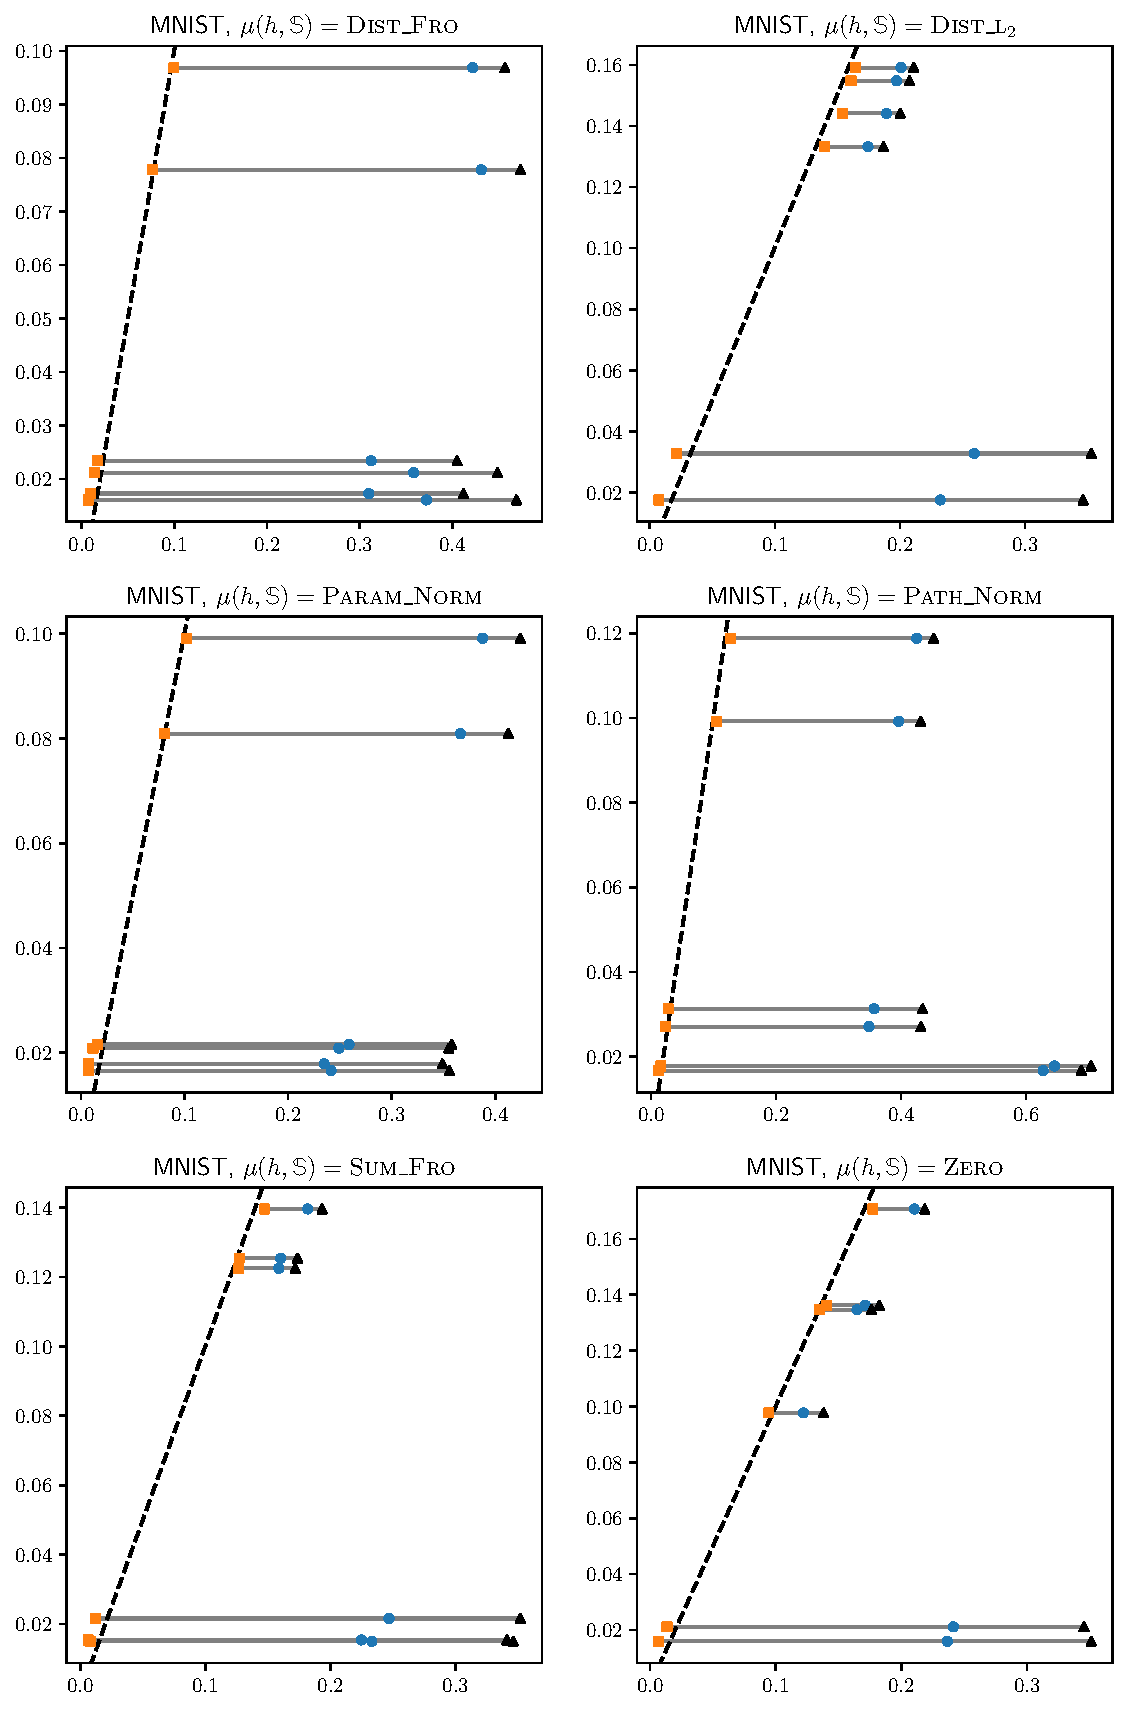
\includegraphics[width=0.77\linewidth]{chapter_7/figures/gap_mnist.pdf}
    \caption[Tightness of \Cref{chap:dis-mu:eq:disintegrated-comp-mcallester-risk,chap:dis-mu:eq:disintegrated-comp-seeger-risk} on MNIST]{
    \looseness=-1
    Scatter plot given a parametric function $\comp(\h, \S)$, where each segment represents a neural network $\h_{\wbf}$ learned with a given $\alpha$, width $H$ and depth $L$.
    For each segment, there is a corresponding orange square and a blue circle.
    The orange squares corresponds to the empirical risk $\Risk_{\dS}(\h)$ (x-axis) and test risk $\Risk_{\dT}(\h)$ (y-axis).
    The blue circle \resp the black triangle represents \Cref{chap:dis-mu:eq:disintegrated-comp-seeger-risk} \resp \Cref{chap:dis-mu:eq:disintegrated-comp-mcallester-risk} in the x-axis and the test risk $\Risk_{\dT}(\h)$ in the y-axis.
    The dashed line is the identity function.
    }
    \label{chap:dis-mu:fig:gap-mnist}
\end{figure}

\begin{figure}
    \centering
    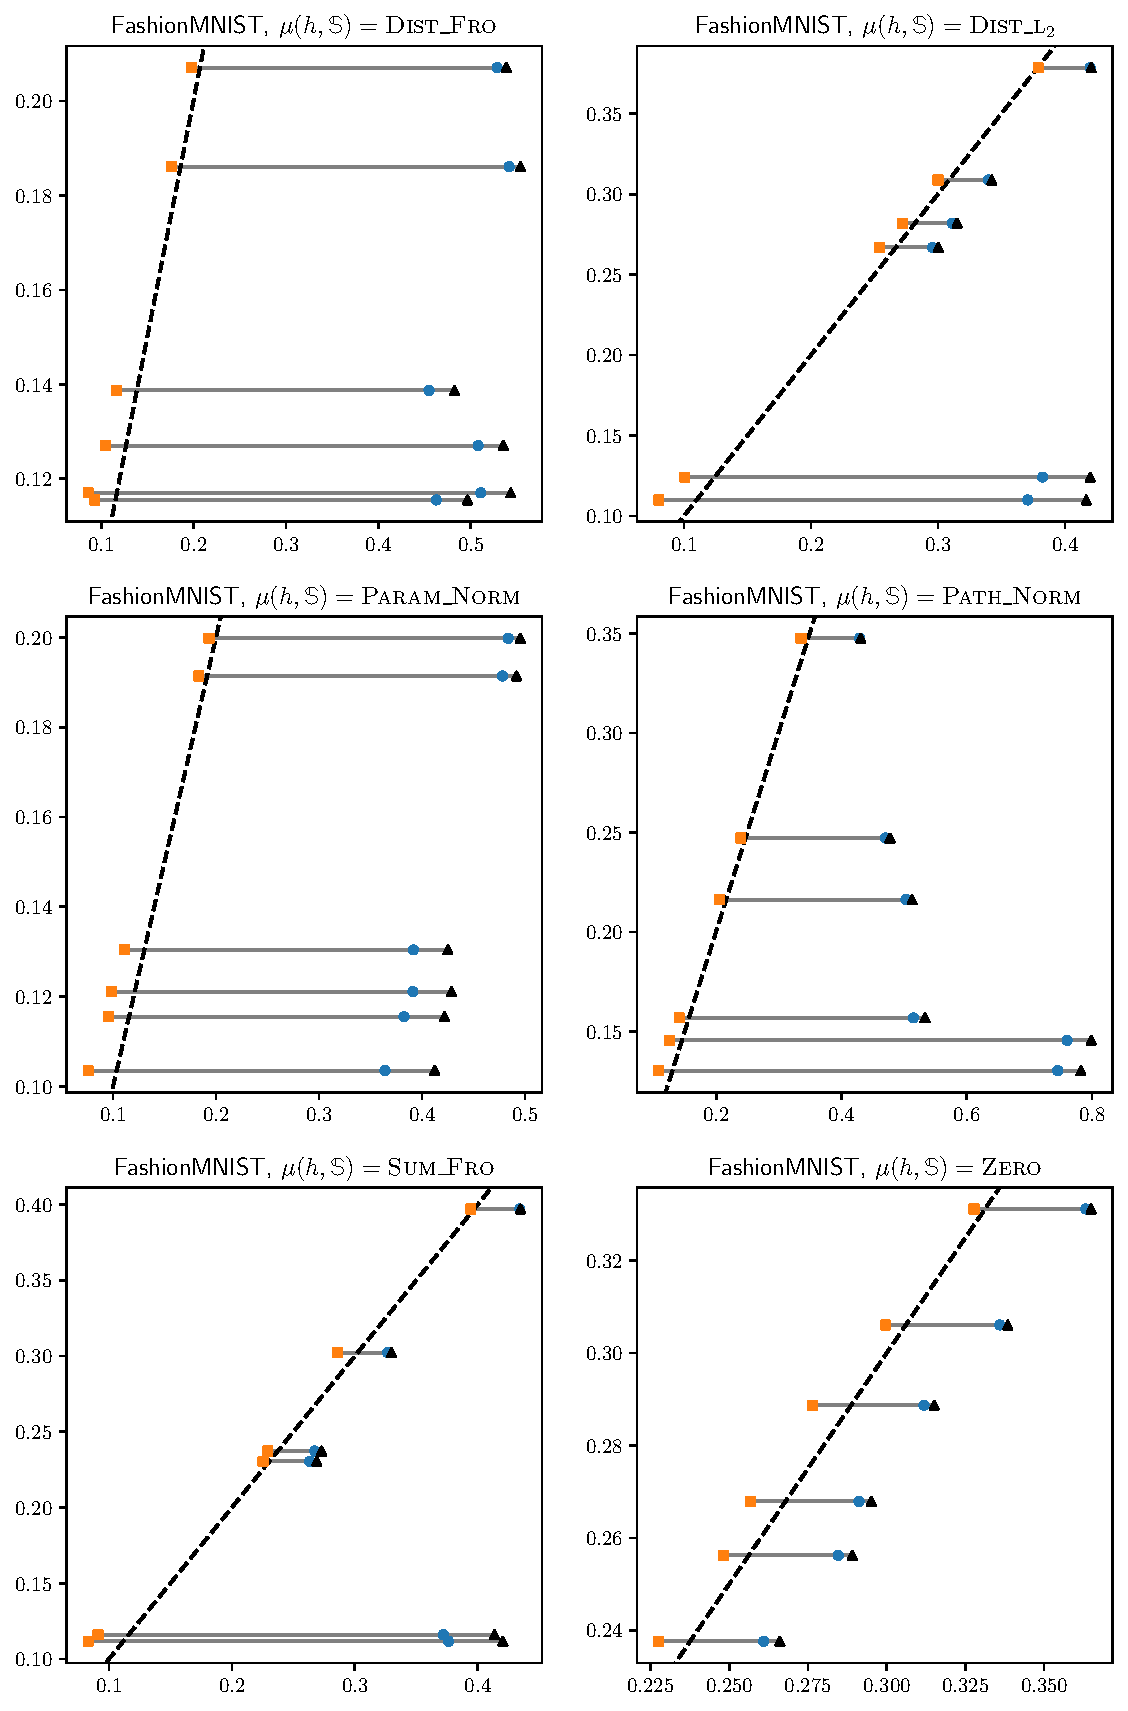
\includegraphics[width=0.77\linewidth]{chapter_7/figures/gap_fashion.pdf}
    \caption[Tightness of \Cref{chap:dis-mu:eq:disintegrated-comp-mcallester-risk,chap:dis-mu:eq:disintegrated-comp-seeger-risk} on FashionMNIST]{
    \looseness=-1
    Scatter plot given a parametric function $\comp(\h, \S)$, where each segment represents a neural network $\h_{\wbf}$ learned with a given $\alpha$, width $H$ and depth $L$.
    For each segment, there is a corresponding orange square and a blue circle.
    The orange squares corresponds to the empirical risk $\Risk_{\dS}(\h)$ (x-axis) and test risk $\Risk_{\dT}(\h)$ (y-axis).
    The blue circle \resp the black triangle represents \Cref{chap:dis-mu:eq:disintegrated-comp-seeger-risk} \resp \Cref{chap:dis-mu:eq:disintegrated-comp-mcallester-risk} in the x-axis and the test risk $\Risk_{\dT}(\h)$ in the y-axis.
    The dashed line is the identity function.
    }
    \label{chap:dis-mu:fig:gap-fashion}
\end{figure}

\begin{figure}
    \centering
    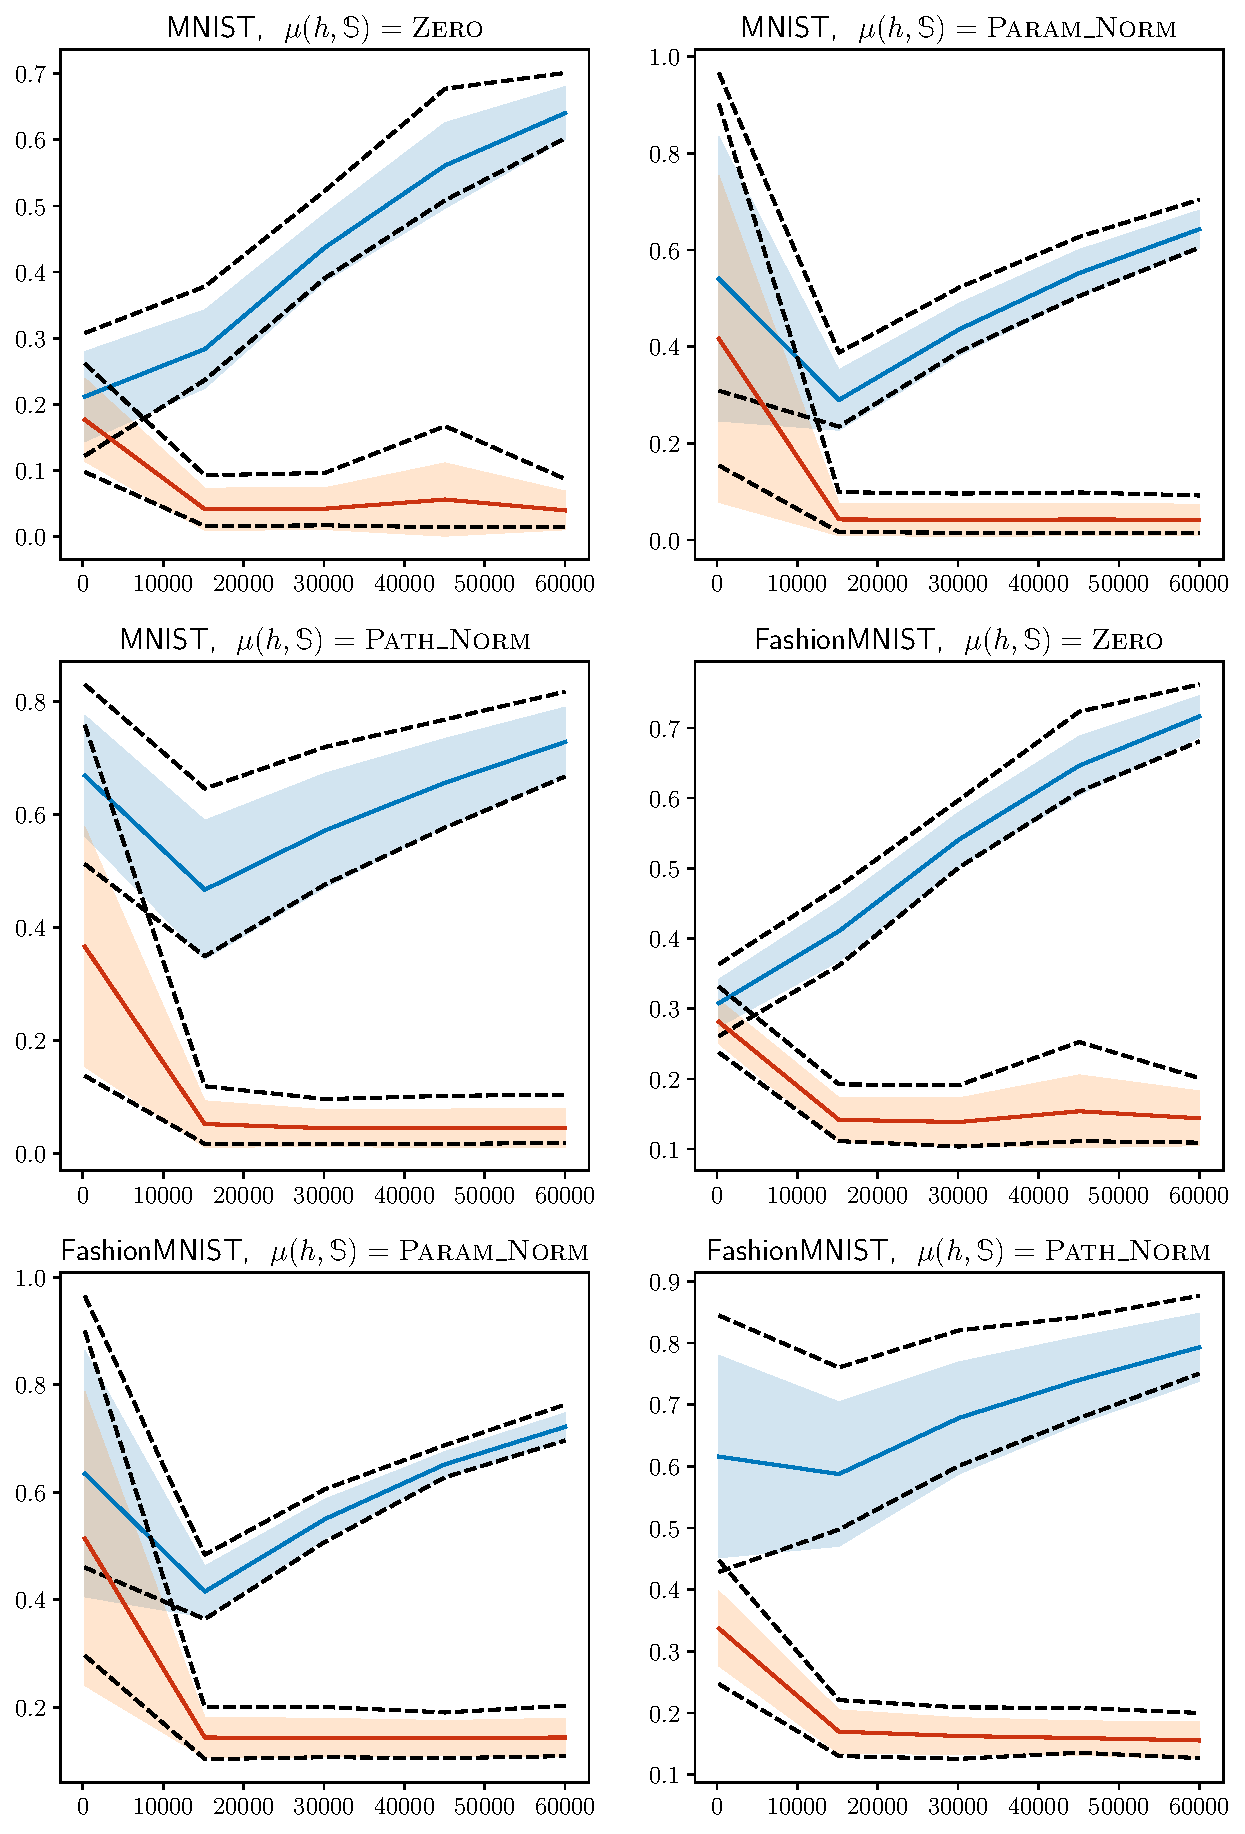
\includegraphics[width=0.82\linewidth]{chapter_7/figures/influence_alpha_summary.pdf}
    \caption[Influence of the Parameter $\alpha$]{
    \looseness=-1
    Influence of the parameter $\alpha$ (in the x-axis) for three parametric functions: $\zero$, $\paramnorm$, and $\pathnorm$ for MNIST and FashionMNIST.
    The bound values are represented in blue and the test risk in red. 
    The two (solid) lines are the mean values computed on the depths and widths; the shadows are the standard deviation.
    The dashed lines are the minimum and the maximum values.
    }
    \label{chap:dis-mu:fig:influence-alpha}
\end{figure}

\begin{figure}
    \centering
    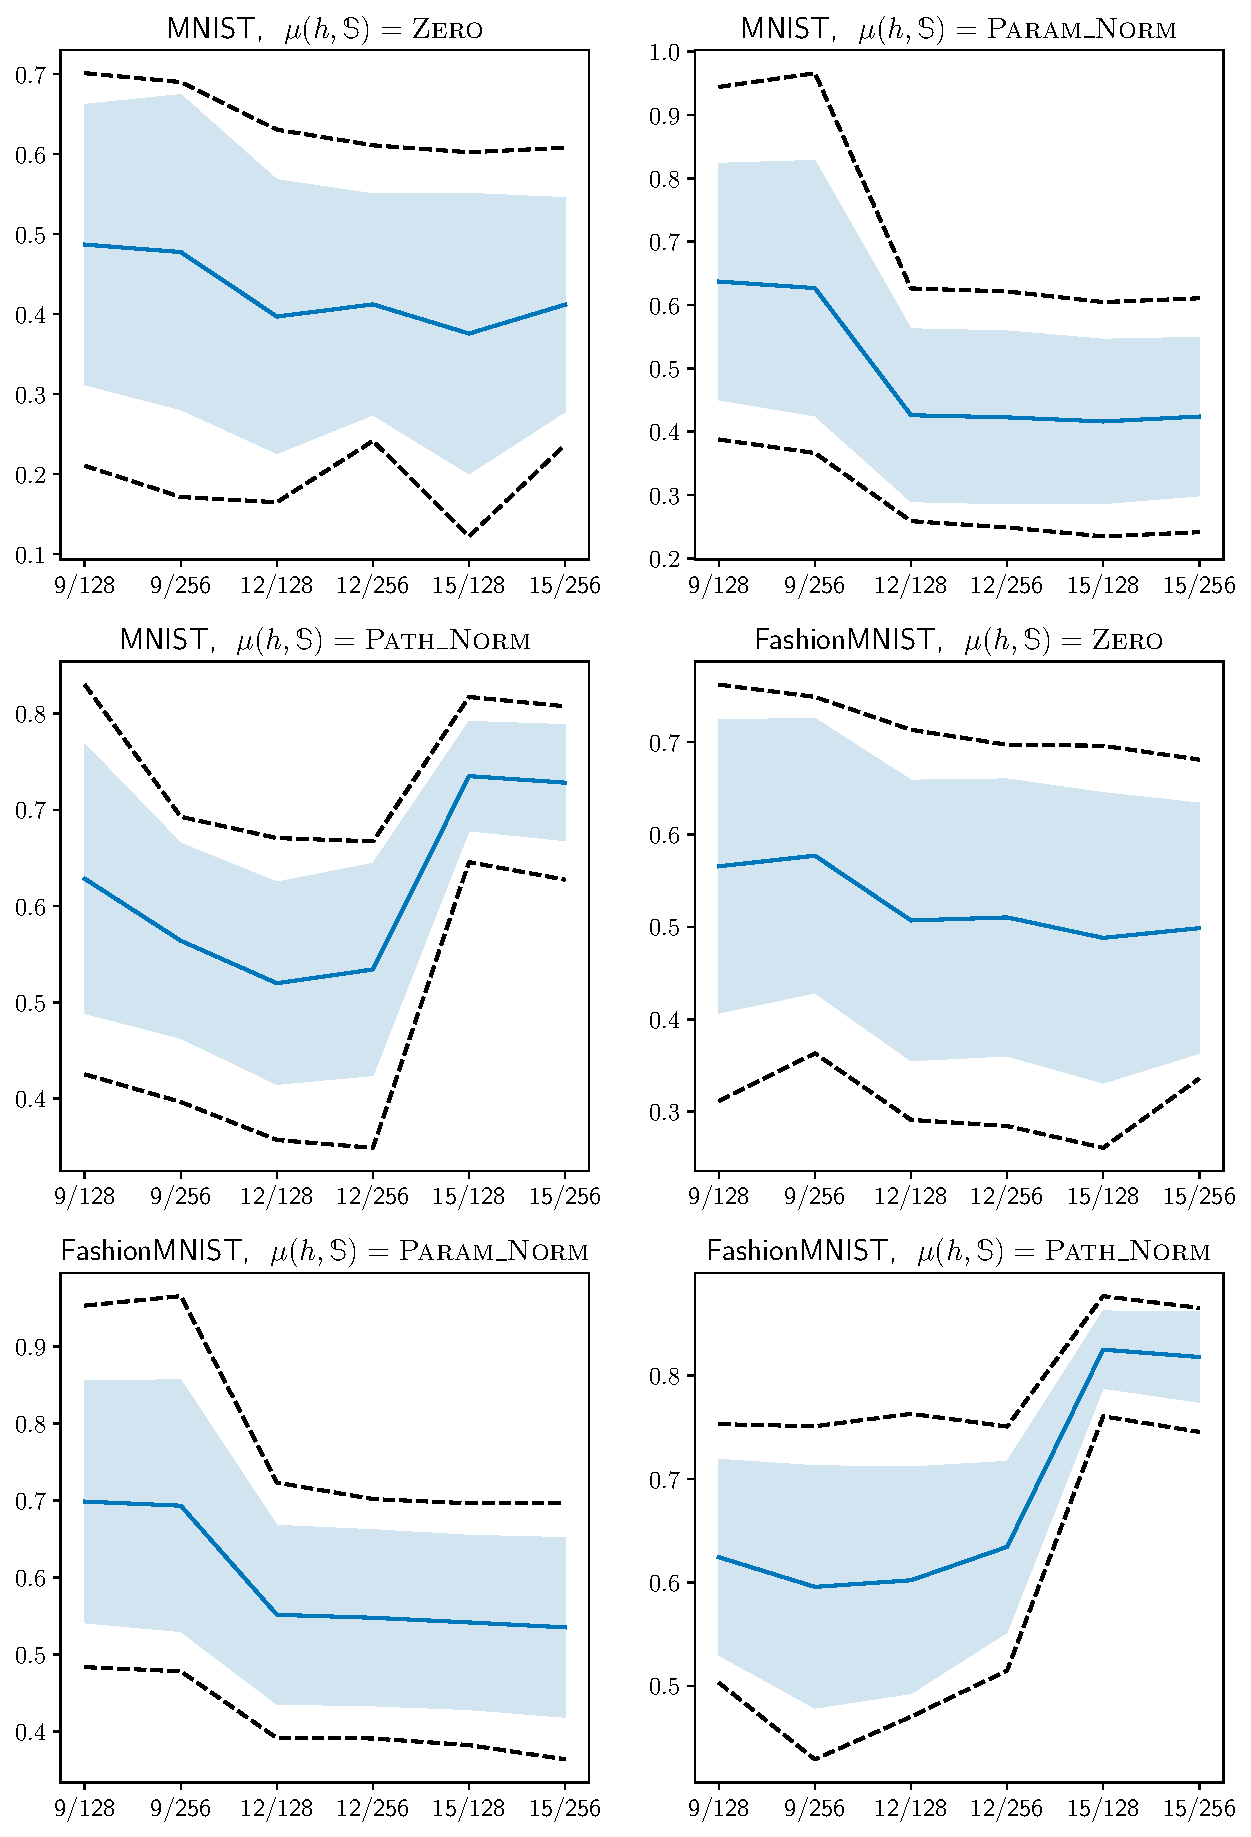
\includegraphics[width=0.82\linewidth]{chapter_7/figures/influence_depth_summary.pdf}
    \caption[Influence of the Depth/Width]{
    \looseness=-1
    Influence of the depth and the width (in the x-axis as ``depth/width'') for three parametric functions: $\zero$, $\paramnorm$, and $\pathnorm$ for MNIST and FashionMNIST.
    The (solid) lines are the mean values computed on the different values of $\alpha$; the shadows are the standard deviation. 
    The dashed lines are the minimum and the maximum values.
    }
    \label{chap:dis-mu:fig:influence-depth}
\end{figure}

For each parametric function $\comp()$, we report in \Cref{chap:dis-mu:fig:gap-mnist,chap:dis-mu:fig:gap-fashion}, the test risks $\Risk_{\dT}(\h)$ and the values of the tightest bound (\wrt $\alpha$) associated to \Cref{chap:dis-mu:eq:disintegrated-comp-seeger-risk,chap:dis-mu:eq:disintegrated-comp-mcallester-risk} for different parameters (depth $L$, width $H$).
First of all, we can remark that certain empirical risks are high.
This is due to the sampling of the hypothesis $\h$ from the distribution $\AQ$: the hypothesis does not necessarily minimizes the objective function $\h \mapsto \Risk_{\dS}(\h){+}\frac{1}{\alpha}\comp(\h, \S)$.
We can nevertheless observe that the bounds' values are higher when the empirical risk $\Risk_{\dT}(\h)$ is low.
This can be explained by the fact that $\LB\alpha\Risk_{\dS}(\h{'})  + \comp(\h'\!,\S)\RB - \LB\alpha\Risk_{\dS}(\h)+\comp(\h,\S)\RB$ is large in this case.
When the empirical risks are a bit higher, the bounds become tighter for certain parametric function such as $\distltwo$, $\sumfro$. 
This confirms that there is an interest to use a parametric function that captures information on the model during the training phase.

\subsubsection{Influence of the Parameter $\alpha$}
\label{chap:dis-mu:sec:influence-alpha}

We analyze the influence of the parameter $\alpha$ in \Cref{chap:dis-mu:eq:disintegrated-comp-seeger-risk}.
To do so, we plot an overview of the evolution for the bounds and the test risks $\Risk_{\dT}(\h)$; the details are reported in \Cref{ap:dis-mu}. 
For each parameter $\alpha$, we plot in \Cref{chap:dis-mu:fig:influence-alpha} the mean, the standard deviation, the minimum and the maximum for the different parameters (depth and width).
In general, the bound increases when the $\alpha$ tends to $\m$ but the test risks $\Risk_{\dT}(\h)$ are less prone to variations.
Indeed, the higher the parameter $\alpha$, the more concentrated around the minimizers the hypothesis will be sampled.
On the contrary, for a small $\alpha$ (\eg, $\alpha=\sqrt{\m}$), the Gibbs distribution defined in \Cref{chap:dis-mu:eq:gibbs-distribution} is less concentrated making the test risks potentially high with a tighter generalization bound.

\subsubsection{Influence of the Depth/Width}
\label{chap:dis-mu:sec:influence-depth}

In \Cref{chap:dis-mu:fig:influence-depth}, we show an overview of the evolution of \Cref{chap:dis-mu:eq:disintegrated-comp-seeger-risk} with respect to the depth and the width.
More precisely, we report the mean, the standard deviation, the minimum and the maximum values for three parametric functions ($\zero$, $\paramnorm$, and $\pathnorm$).

Interestingly, the evolution of the bounds highly depends on the chosen parametric function $\comp()$. 
For instance, the bound increases with $\pathnorm$ when the depth and the width increase.
This is in contrast with $\paramnorm$ that decreases when the number of parameters increases.
This shows the interest of our framework: considering a user-specified complexity measure $\PhiComp()$ can help to understand the generalization of over-parameterized models (that are sampled from $\AQ$).

\section{Comparison with the Generalization Bounds of the Literature}
\label{chap:dis-mu:sec:comparison}

In this section, we theoretically compare generalization bounds with arbitrary complexity measures compared to literature's bounds. 
We prove that our bound generalizes the uniform-convergence and the algorithmic-dependent bounds.
Additionally, we show that the algorithmic-dependent bounds can be tighter than uniform-convergence bounds.
To do so, we propose in \Cref{chap:dis-mu:proposition:disintegrated,chap:dis-mu:proposition:uc,chap:dis-mu:proposition:algorithmic} a reinterpretation of the high probability bounds in terms of sets.
Additionally, we prove in \Cref{chap:dis-mu:corollary:dis-uc,chap:dis-mu:corollary:dis-algo} two special cases of our bound in \Cref{chap:dis-mu:theorem:disintegrated-comp} that generalizes the two types of bounds.

\subsection{Bounds with Arbitrary Complexity Measures}

In order to compare our framework with the uniform-convergence and the algorithmic-dependent bounds, we translate \Cref{chap:dis-mu:def:comp-bound} into the following set-theoretic result.

\begin{restatable}[Set-theoretic view of \Cref{chap:dis-mu:def:comp-bound}]{proposition}{propositiondisintegrated}\label{chap:dis-mu:proposition:disintegrated}
Let $\phi: [0,1]^2{\to}\Rbb$ be a generalization gap and assume that there exists a function $\PhiComp: \H{\times}(\X{\times}\Y)^\m{\times}(0,1]\to\Rbb$ fulfilling \Cref{chap:dis-mu:def:comp-bound}.
Under these conditions, with $\setD {=} \Big\{ (\h, \S)\!\in\! \H{\times}(\X{\times}\Y)^\m :  \phi(\Risk_{\D}(\h), \Risk_{\dS}(\h))\!\le\!\PhiComp(\h, \S, \delta) \Big\}$, and  $\PP_{\S\sim\D^\m, h\sim\AQ}\LB (\h, \S)\in\setD \RB\ge  1{-}\delta$, we have
\begin{align*}
    \text{\Cref{chap:dis-mu:eq:comp-bound}} \iff\ &\forall (\h, \S)\in \setD,\  \phi(\Risk_{\D}(\h), \Risk_{\dS}(\h)) \le \PhiComp(\h, \S, \delta)\\
 \iff\ &  {\textstyle\sup_{(\h, \S)\in \setD}} \Big\{\phi(\Risk_{\D}(\h), \Risk_{\dS}(\h)) - \PhiComp(\h, \S, \delta) \Big\} \le 0.
\end{align*}
\end{restatable}
\begin{noaddcontents}\begin{proof}
Deferred to~\Cref{ap:dis-mu:sec:proof-prop-disintegrated}.
\end{proof}\end{noaddcontents}
For a given confidence $\delta$, with probability at least $1{-}\delta$,
the bound is then valid for all $(\h, \S)$ belonging to a (reduced) set $\setD \!\subseteq\! \H{\times}(\X{\times}\Y)^\m$.
In other words, the bound always holds for a given hypothesis and learning sample $(\h, \S)\!\in\!\setD$, and its value depends on these $\h$ and $\S$.  
The generality of our framework can thus generalize both uniform convergence and algorithmic dependent bounds as we see in the rest of this section. 

\subsection{Uniform Convergence Bounds}

\looseness=-1
Uniform-convergence-based bounds were the first type of generalization bounds to be introduced, notably in \citet{VapnikChervonenkis1971} using the VC-dimension as complexity.
Other bounds were later developed based on the Gaussian/Rademacher complexity~\citep{BartlettMendelson2002} instead.
We recall the definition of this type of bounds encountered in \Cref{chap:intro}.

\definitionUC*

Remember that this definition encompasses different complexity measures, such as $\PhiUC(\delta){=}\rad(\H) {+} \sqrt{\tfrac{1}{2\m}\ln\frac{1}{\delta}}$ in \Cref{chap:intro:theorem:rademacher}, or $\PhiUC(\delta){=}\sqrt{\frac{1}{m}2\vc(\H)\ln\frac{em}{\vc(\H)}}{+}\sqrt{\tfrac{1}{2\m}\ln\frac{1}{\delta}}$ described in \Cref{chap:intro:theorem:vc-dim}.
For ease of comparison, we refine and reinterpret this type of bounds in a set-theoretic manner as follows.
This result has been originally remarked by \citet{NagarajanKolter2019} (but not proved).

\begin{restatable}[Set-theoretic View of Uniform Convergence Bounds]{proposition}{propositionuc}\label{chap:dis-mu:proposition:uc}
Let $\phi: [0,1]^2{\to}\Rbb$ be a generalization gap and assume that there exists a function $\PhiUC: (0,1]\to\Rbb$ fulfilling \Cref{chap:intro:def:uc}.
Under these conditions, with $\displaystyle\setUC = \big\{ \S\in (\X{\times}\Y)^\m \!:\! \forall \h\in\H,\, \phi(\Risk_{\D}(\h), \Risk_{\dS}(\h)) \le \PhiUC(\delta) \big\}$, and $\PP_{\S\sim\D^\m}\LB \S{\in}\setUC \RB{\ge}  1{-}\delta$, we have
\begin{align*}
    \text{\Cref{chap:intro:eq:uc}} &\iff \forall \S \in \setUC,\   \forall h\!\in\! \H,\, \phi(\Risk_{\D}(\h), \Risk_{\dS}(\h)) \le \PhiUC(\delta)\\
    &\iff \sup_{\S\in\setUC}\sup_{h\in\H}\big\{\phi(\Risk_{\D}(\h), \Risk_{\dS}(\h))\big\}\! \le\! \PhiUC(\delta).
\end{align*}
\end{restatable}
\begin{noaddcontents}\begin{proof}
Deferred to~\Cref{ap:dis-mu:sec:proof-prop-uc}.
\end{proof}\end{noaddcontents}

\Cref{chap:dis-mu:proposition:uc} is, in fact, a reinterpretation of PAC generalization bounds by identifying the subset $\setUC {\subseteq} (\X{\times}\Y)^\m$ for which the upper bound $\PhiUC(\delta)$ is valid.
This highlights their worst-case nature:
given a confidence $\delta$, the generalization gap $\phi(\Risk_{\D}(\h), \Risk_{\dS}(\h))$ is upper-bounded by a complexity measure $\PhiUC(\delta)$ for all $(\h,\S)\!\in\!\H{\times}\setUC$.
To get a bound holding with probability at least $1{-}\delta$, 
since the complexity $\PhiUC(\delta)$ does not depend on $\h$ or $\S$, the complexity has to upper-bound the worst hypothesis $\h\!\in\!\H$ and the worst learning sample $\S\!\in\!\setUC$. 
As a consequence, $\PhiUC(\delta)$ is lower-bounded by $\sup_{\S\in\setUC}\sup_{h\in\H}\phi(\Risk_{\D}(\h), \Risk_{\dS}(\h))$.
As we have seen in \Cref{chap:dis-mu:proposition:disintegrated}, our bound is more permissive than the uniform convergence bounds since the upper bound can depend on the learning sample $\S$ and the hypothesis $\h$.
Hence, this dependence on $\S$ and $\h$ allows us to retrieve the uniform convergence bounds with our framework.
Indeed, from \Cref{chap:dis-mu:theorem:disintegrated-comp}, we can obtain the following generalization bound.

\begin{restatable}[Uniform Convergence Bound from \Cref{chap:dis-mu:theorem:disintegrated-comp}]{corollary}{corollarydisuc} \label{chap:dis-mu:corollary:dis-uc}
Let $\phi\!:\! [0,1]^2{\to}\Rbb$ be the generalization gap and assume that there exists a function $\PhiUC: (0,1]\to\Rbb$ fulfilling \Cref{chap:intro:def:uc} such that $\PhiUC(\delta) \ge \ln\!\LB \frac{4}{\delta^2} \EE_{\S'\!{\sim}\D^\m}\EE_{\h'\!{\sim}\P} \exp\LP\phi(\Risk_{\D}(\h{'}),\Risk_{\dS'}(\h'))\RP\RB$.
For any $\D$ on $\X\times\Y$, for any hypothesis set $\H$, for any $\delta\in(0, 1]$, we have
\begin{align*}
    \PP_{\S\sim\D^\m, \h\sim\AQ}\!\Bigg[ \phi(\Risk_{\D}(\h), \Risk_{\dS}(\h)) \le \PhiUC(\delta) \Bigg] \ge 1-\delta.
\end{align*}
\end{restatable}
\begin{noaddcontents}\begin{proof}
Deferred to~\Cref{ap:dis-mu:sec:proof-cor-dis-uc}.
\end{proof}\end{noaddcontents}

Note that, to prove \Cref{chap:dis-mu:corollary:dis-uc}, we require an additional assumption: a lower-bound on $\PhiUC(\delta)$.
When the generalization gap is $\phi(\Risk_{\D}(\h), \Risk_{\dS}(\h)){=}2m[\Risk_{\D}(\h){-}\Risk_{\dS}(\h)]^2$ or $\phi(\Risk_{\D}(\h), \Risk_{\dS}(\h)){=}\kl[\Risk_{\dS}(\h)\|\Risk_{\D}(\h)]$, the lower bound is $\ln\frac{8\sqrt{\m}}{\delta^2}$ (see \Cref{chap:dis-mu:corollary:disintegrated-comp}) which is low enough to be a worst-case upper-bound.
To sum up, our framework is general enough to retrieve classical uniform convergence bounds (under the mild assumption) such that the ones based on the Rademacher complexity (\Cref{chap:intro:def:rademacher}) or the VC-Dimension (\Cref{chap:intro:def:vc-dim}).
In practice, the sampling involved in the bound of \Cref{chap:dis-mu:corollary:dis-uc} is not necessary: the bound holds for all hypothesis $\h\in\H$ with high probability.
More precisely, for $\PhiUC(\h,\S,\delta)=\PhiUC(\delta)$, the set $\setUC$ in \Cref{chap:dis-mu:proposition:uc} can be seen as a subset of $\setD$ since
\begin{align*}
    \Big\{ \S\in(\X{\times}\Y)^\m \;\Big|\; \forall \h\in\H,\ (\S,\h)\in\setD \Big\} = \setUC.
\end{align*}
Hence, for a well-behaved learning sample $\S$, \ie, for $\S\in\setUC$, we have that
\begin{align*}
    \EE_{\h\in\AQ}\indic\Big[ \phi(\Risk_{\D}(\h), \Risk_{\dS}(\h)) \le \PhiUC(\delta) \Big] &= \indic\LB \sup_{\h\in\H}\phi(\Risk_{\D}(\h), \Risk_{\dS}(\h)) \le \PhiUC(\delta) \RB\\
    &= 1,
\end{align*}
which gives a valid bound for all $\h\in\H$ without sampling.
This generality of this framework does not apply uniquely to these type of bounds. 
We can obtain a result similar for the algorithmic-dependent bounds that can be tighter than the uniform-convergence-based bounds. 

\subsection{Algorithmic-Dependent Bounds}

\looseness=-1
The upper bound $\PhiUC(\delta)$ can generally be improved by considering algorithmic-dependent bounds~\citep{BousquetElisseeff2002, XuMannor2012}.
In this case, only the output $\h_{\S}$ of a learning algorithm given $\S$ is studied: we only bound the generalization gap $\phi(\Risk_{\D}(\h_{\S}), \Risk_{\dS}(\h_{\S}))$ specific to $\h_{\S}$ (here,  $\H{=}\{\h_{\S}\}_{\S\in(\X{\times}\Y)^\m}$).
The definition of such bounds encountered in \Cref{chap:intro} is recalled in the following.

\definitionALGODEP*

Similarly to the uniform convergence bounds, these bounds can be reformulated through a similar set-theoretic lens stated in the following proposition.

\begin{restatable}[Set-theoretic View of Algorithmic Dependent Bounds]{proposition}{propositionalgodep}\label{chap:dis-mu:proposition:algorithmic}
\looseness=-1
Let $\phi: [0,1]^2{\to}\Rbb$ be a generalization gap and assume that there exists a function $\PhiA: (0,1]\to\Rbb$ fulfilling \Cref{chap:intro:def:algo}.
Under these conditions, with $\setA = \big\{ \S\in (\X{\times}\Y)^\m \!:\! \phi(\Risk_{\D}(\h_{\S}), \Risk_{\dS}(\h_{\S}))\le\PhiA(\delta) \big\}$ and $\PP_{\S{\sim}\D^\m}\!\LB \S\in\setA \RB\ge  1{-}\delta$, we have
\begin{align*}
    \text{\Cref{chap:intro:eq:algo}}\ &\iff \forall\S\in\setA,  \phi(\Risk_{\D}(\h_{\S}), \Risk_{\dS}(\h_{\S})) \le \PhiA(\delta)\\
    &\iff {\textstyle \sup_{\S\in\setA}} \phi(\Risk_{\D}(\h_{\S}), \Risk_{\dS}(\h_{\S})) \le \PhiA(\delta). 
\end{align*}
\end{restatable}
\begin{noaddcontents}\begin{proof}
Deferred to~\Cref{ap:dis-mu:sec:proof-prop-algo}.
\end{proof}\end{noaddcontents}
Since the upper bound $\PhiA(\delta)$ is at least $\sup_{\S\in\setA}\phi(\Risk_{\D}(\h_{\S}), \Risk_{\dS}(\h_{\S}))$, this result has the potential to lead to tighter guarantees than the uniform convergence ones.
For example, when $\H {=} \LC \h_{\S}\RC_{\S\in(\X{\times}\Y)^\m}$ is an algorithmic-dependent hypothesis set and $\setA\!\subseteq\!\setUC$.
The complexity measure $\PhiA(\delta)$ can potentially be smaller than $\PhiUC(\delta)$ since we have the inequality 
\begin{align*}
\sup_{\S\in\setA}\phi(\Risk_{\D}(\h_{\S}), \Risk_{\dS}(\h_{\S})) &\le \sup_{\S\in\setUC}\phi(\Risk_{\D}(\h_{\S}), \Risk_{\dS}(\h_{\S}))\\
&\le \sup_{\S\in\setUC}\sup_{\h\in\H}\phi(\Risk_{\D}(\h), \Risk_{\dS}(\h))\\
&\le \PhiUC(\delta).
\end{align*}
Even though these type of bounds can be tighter, it is still not as permissive as our framework.
Indeed, the upper bound $\PhiA(\delta)$ is a constant \wrt the hypothesis and the learning sample (like the uniform convergence bounds).
Hence, since our bound can depend on the learning sample $\S$ and the hypthesis $\h$, we retrieve the algorithmic-dependent bounds illustrating the generality of our framework (similarly to \Cref{chap:dis-mu:corollary:dis-uc}).
The result is in the following corollary.

\begin{restatable}[Algorithmic-dependent Bound from \Cref{chap:dis-mu:theorem:disintegrated-comp}]{corollary}{corollarydisalgo} \label{chap:dis-mu:corollary:dis-algo}
Let $\phi\!:\! [0,1]^2{\to}\Rbb$ be the generalization gap and assume that there exists a function $\PhiA: (0,1]\to\Rbb$ fulfilling \Cref{chap:intro:def:algo} such that $\PhiA(\delta) \ge \ln\!\LB \frac{4}{\delta^2} \EE_{\S'\!{\sim}\D^\m}\EE_{\h'\!{\sim}\P} \exp\LP\phi(\Risk_{\D}(\h{'}),\Risk_{\dS'}(\h'))\RP\RB$.
For any $\D$ on $\X\times\Y$, for any hypothesis set $\H$, for any $\delta\in(0, 1]$, we have
\begin{align*}
    \PP_{\S\sim\D^\m, \h\sim\AQ}\!\Bigg[ \phi(\Risk_{\D}(\h), \Risk_{\dS}(\h)) \le \PhiA(\delta) \Bigg] \ge 1-\delta.
\end{align*}
\end{restatable}
\begin{noaddcontents}\begin{proof}
Deferred to~\Cref{ap:dis-mu:sec:proof-corollary-algo}.
\end{proof}\end{noaddcontents}

Compared to the bounds of \Cref{chap:intro:def:algo}, \Cref{chap:dis-mu:corollary:dis-algo} still involves the expectation over the hypotheses. 
Hopefully, the bound holds with high probability for the data-dependent hypothesis $\h_{\S}$ (see \Cref{chap:dis-mu:proposition:algorithmic}).
Hence, when using \Cref{chap:dis-mu:corollary:dis-algo}'s bound the sampling is not necessary since we can consider the bound only for the hypothesis of interest, \ie, $\h_{\S}$ for all $\S\in\setA$ which holds with high probability.
In other words, when $\PhiComp(\h,\S,\delta) = \PhiA(\delta)$, the set $\setA$ in \Cref{chap:dis-mu:proposition:algorithmic} can be seen as a subset of $\setD$ since
\begin{align*}
    \Big\{ \S\in(\X{\times}\Y)^\m \;\Big|\; (\S,\h_{\S})\in\setD \Big\} = \setA.
\end{align*}

In summary, the framework proposed in this chapter is powerful enough to cover uniform-convergence-based bound and algorithm-dependent bounds with the integration of a complexity measure. 
To the best of our knowledge, this has not been identified before and we think this is something novel.

\section{Conclusion and Summary}
\label{chap:dis-mu:sec:conclu}

In this chapter, we provide a novel generalization bound that involves arbitrary complexity measures, unlike classical learning theory frameworks (for which the complexity is imposed by the framework itself).
These measures incorporate a data and model dependent function, that allow us to generalize the previous framework introduced in the literature (see \Cref{chap:intro:sec:bound}).
Importantly, to the best of our knowledge, our framework provides for the first time theoretical guarantees for the many arbitrary complexity measures used in practice in machine learning, \eg,  for regularization purposes.\\

The limitation of this work is clearly that the hypothesis is obtained from a distribution difficult to use, namely the Gibbs distribution.
Indeed, one sampling from the Gibbs distribution is performed by an algorithm such as \Cref{chap:dis-mu:algo:sto-mala}.
Hopefully, the generality of this framework allows to avoid the sampling if we consider uniform-convergence-type bounds as in \Cref{chap:dis-mu:corollary:dis-uc}.
We can easily imagine continuing in this research direction.
For instance, we can try to get rid of the supremum \wrt to the hypothesis set $\H$ in the Rademacher complexity (\Cref{chap:intro:def:rademacher}) since it it hard to compute.

We hope that our results foster research in the topic and the development of new complexity measures for specific neural network architectures and for specific learning tasks.
Indeed, we believe that this work paves the way to new research directions that tries to bridge the statistical learning theory and the practice.
Indeed, finding a good complexity measures becomes a practical matter since any complexity measure can be integrated in our framework.\\

In general, this thesis explores the disintegrated bounds in order to explain better the generalization of over-parameterized models that is largely misunderstood. 
We believe that this type of bounds is not the only promising type of bounds that can explain the generalization phenomenon.
In \Cref{part:conclusion}, we give an idea of research direction to explore other type of generalization bounds.


\part{Conclusion and Perspectives}
\label{part:conclusion}

%\chapter*{Conclusion and Perspectives}
\addcontentsline{toc}{chapter}{Conclusion and Perspectives}
\label{chap:conclu}

\section*{Conclusion}

This thesis mainly derives self-bounding algorithms that learn a model minimizing a (disintegrated) PAC-Bayesian generalization bound.
This type of algorithm has received little attention in the machine learning literature and we propose some contributions in various contexts.\\

Indeed, \Cref{part:contrib-pac-bayes} is dedicated to deriving self-bounding algorithms in the context of majority vote classifiers.
In \Cref{chap:mv-robustness,chap:mv}, we derived self-bounding algorithms for the majority vote classifier in two different settings: the adversarial robustness and the classical supervised setting.
More precisely, \Cref{chap:mv-robustness}'s self-bounding algorithms robustify the majority votes against small perturbations.
While \Cref{chap:mv} minimizes the majority vote's true risk through the PAC-Bayesian C-Bounds considered as challenging to optimize~\citep{LorenzenIgelSeldin2019,MasegosaLorenzenIgelSeldin2020}.
However, as shown in \Cref{chap:mv-sto}, the majority vote's self-bounding algorithms considered, \eg, in \Cref{chap:mv}, do not minimize tight generalization bounds on the true risk, even for simple tasks.
Hence, to overcome this drawback, \Cref{chap:mv-sto} introduces the stochastic majority vote, which samples a majority vote for each prediction.
Considering such a majority vote allows us to obtain tight generalization bounds.
Additionally, we derive a self-bounding algorithm that directly minimizes the risk of the stochastic majority vote in this context.

However, the risk of a stochastic model is the expected risk of the hypotheses, which requires certain assumptions to be computed while we may be only interested in assessing the behavior of only one hypothesis in some situations.
Hence, to overcome this drawback, we consider in \Cref{part:contrib-disintegrated} the {\it disintegrated} PAC-Bayesian bounds.
\Cref{chap:dis-pra} provides new bounds based on the Rényi divergence that are more easily optimizable (for self-bounding algorithms) than the ones of the literature~\citep[\ie, ][]{BlanchardFleuret2007,Catoni2007,RivasplataKuzborskijSzepesvariShaweTaylor2020}.
Even though \citet{RivasplataKuzborskijSzepesvariShaweTaylor2020}'s bound is not easily optimizable, it is a starting point to derive new generalizations bounds.
Indeed, in the last contribution (\Cref{chap:dis-mu}), we leverage \citet{RivasplataKuzborskijSzepesvariShaweTaylor2020}'s disintegrated framework to derive generalization bounds with arbitrary complexity measures.
Such work is fundamental in statistical learning theory: to the best of our knowledge, we are the first to provide generalization bounds that integrate complexity measures that can be defined by the user.
This work allows the machine learning community to consider new generalization bounds by defining a new complexity measure.
Hence, new works can focus on developing new complexity measures to understand better the generalization phenomenon.

\section*{Perspectives}

We present several perspectives following the contributions of this thesis.

\subsection*{Perspectives on the Adversarial Robustness Setting}

As recalled in \Cref{chap:mv-robustness}, in the adversarial robustness setting, we aim to make the model robust to small perturbations in the input.
Indeed, we must ensure that the model does not radically change its prediction for a slight change in the input.
To do so, we consider that the model's output must not change in a ball of a given radius.
This new constraint on the input actually creates a new unknown data distribution that is close, in some sense, to the original unknown data distribution.\\

On the other hand, the transfer learning/domain adaptation\footnote{We refer the reader to \citet{RedkoMorvantHabrardSebbanBennani2019,RedkoMorvantHabrardSebbanBennani2020} for an introduction on domain adaption.} consider two unknown data distributions: a source (\ie, the original) and a target (\ie, a new) distribution.
In this setting, the model learned to solve a task (represented by the source distribution) is adapted to solve a new task (represented by the target distribution).
In some transfer learning scenarios, we assume that we have access to the labels and the inputs obtained from the target distribution, while in unsupervised domain adaptation, only the inputs are considered.
In these two settings, the true risk on the target distribution can be upper-bounded with a generalization bound \citep[see \eg,][]{BenDavidBlitzerCrammerKuleszaPereiraVaughan2010,McNamaraBalcan2017,GalantiWolfHazan2016,GermainHabrardLavioletteMorvant2020}.\\

Besides, it is known that domain adaptation and adversarial robustness are related: unlabeled examples (considered in domain adaptation) can be used to improve the adversarial robustness~\citep{CarmonRaghunathanSchmidtDuchiLiang2019,AlayracUesatoHuangFawziStanforthKohli2019,DengZhangGhorbaniZou2021}.
As a perspective, we propose to investigate the link between these two settings from a theoretical viewpoint.
First, we could explore the connection between the original distribution and the new data distribution induced by the adversarial robustness that can be respectively seen as a source and a target distribution in transfer learning.
Then, this connection may help to leverage transfer learning/domain adaptation generalization bounds to obtain guarantees for the adversarial robustness setting.
The new guarantees might serve to get self-bounding algorithms that {\it (i)} detect out-of-distribution examples\footnote{The examples that are not probable in a given distribution are called out-of-distribution examples.} and {\it (ii)} robustify machine learning models.

\subsection*{Extending the Majority Vote}

In \Cref{part:contrib-pac-bayes}, we consider that the set of voters in the PAC-Bayesian majority vote is fixed.
Hence, only the weights of the majority vote are adapted to fit the examples.
Alternatively, in the (Gradient) Boosting framework~\citep{FreundSchapire1996,Friedman2001}, the voters are greedily learned one by one.
Moreover, in bagging~\citep{Breiman1996} and random forest~\citep{Breiman2001}, no weights are learned while the models are learned separately.
For the Support Vector Machine~\citep{GraepelHerbrichShaweTaylor2005} that can be interpreted as a majority vote, the voters are fixed before learning the weights by choosing a kernel.
As we can remark in these approaches, the voters and the weights are not learned together.
This appears as a limitation since learning the weights and the voters in an end-to-end way can offer a better accurate majority vote.
Hence, one bottleneck has to be overcome: deriving differentiable voters such as differentiable decision stumps.
By doing so, we may improve the voters' diversity while limiting the voters' complexity.
Moreover, the disintegrated PAC-Bayesian framework (developed, \eg, in \Cref{part:contrib-disintegrated}) may be leveraged to derive generalization guarantees for majority votes that depend on the full learning sample.
Again, new generalization bounds can be further used to derive self-bounding algorithms.

\subsection*{Self-bounding and Optimization Algorithms}

The optimization algorithms are key to obtain a good classifier in self-bounding algorithms.
Specifically in \Cref{chap:mv,chap:mv-sto}, we use an optimization algorithm that tune automatically the learning rate, namely COCOB~\citep{OrabonaTommasi2017}.
This approach, belonging to the parameter-free algorithms\footnote{We refer the reader to the ICML 2020 tutorial on Parameter-free online optimization for more details on the parameter-free algorithms.}, is interesting in machine because it has a clear advantage: there is no need to tune the learning rate.
Hence, the parameter-free algorithms could facilitate the use of machine learning approaches for practitioners.
However, we believe that more hyper-parameters can be tuned automatically in parameter-free optimization algorithms such as the batch size, which offers interesting research perspectives.

One idea to derive new parameter-free algorithms is to take inspiration from the federated learning setting.\footnote{Federated learning is a sub-field of machine learning; see \citet{Kairouz2021} for a survey.}
It considers different clients that learn collaboratively in a machine learning model; each client has its own learning sample and does not necessarily share it.
For instance, to learn the model, each client has its own local model and runs an optimization algorithm, to obtain new weights.
The new weights of each local model are aggregated to obtain a global model finally, without exchanging the data; see, \eg, the FedAvg algorithm~\citep[see][]{McMahanMooreRamageHampsonArcas2017}.
A modification must be made to FedAvg to obtain a parameter-free algorithm since each client runs an algorithm with different values of hyper-parameters. 
The aggregation of the weights can take different forms, such as a convex combination. 
With this latter type of aggregation, the PAC-Bayesian theory might be helpful to obtain convergence guarantees.

\subsection*{Towards a New Type of Generalization Bounds}

The PAC-Bayesian theory considers that the data and the models are respectively sampled from two probability distributions: the unknown distribution and the posterior distribution.
While it can be convenient to derive generalization guarantees on a single model sampled from the posterior distribution, we are usually interested in a model that is not necessarily sampled.

Instead of considering the posterior distribution on the models, one could consider a distribution on the label set conditioned on the input.
If this distribution is somehow learned from the learning sample, it can be seen as a machine learning model.
Thanks to this distribution, we could derive generalization bounds on the expected loss when the labels are sampled from the new data-dependent distribution (associated with a classifier).
We can for example hope to obtain a bound dependent on the mutual information between the predictions and the labels.
Roughly speaking, mutual information measures how much information on the labels is contained in the predictions.
Hence, it can be seen as a complexity measure of the data-dependent distribution (representing the classifier).
For instance, this quantity has been considered in the information bottleneck framework of~\citet{TishbyPereiraBialek2000}.
Besides, the training of neural networks has been studied through this framework~\citep[see][]{ShwartzZivTishby2017}\pokeball

% ----------------------------------------------------------------------------------------------- %

\appendix
\part{Appendix}

\chapter{Some Mathematical Tools}
\addtextlist{loe}{Appendix}

\section{\textsc{Jensen}'s Inequality}

\begin{theorem}[\textsc{Jensen}'s Inequality]
Let $X$ a random variable following a probability distribution $\nu$ with $f$ a real-valued measurable convex function, we have
\begin{align*}
    f\LP\EE_{X\sim\nu}\LB X\RB\RP \le \EE_{X\sim\nu}\Big[ f\LP X\RP \Big].
\end{align*}
\label{ap:tools:theorem:jensen}
\end{theorem}
\begin{noaddcontents}\begin{proof}
Since $f()$ is a convex function, the following inequality holds, \ie, we have
\begin{align*}
\forall X',\quad a\LP X' - \EE_{X\sim\nu}\LB X\RB\RP \le f(X') - f\LP\EE_{X\sim\nu}\LB X\RB\RP,
\end{align*}
where $a$ is the tangent's slope.
By taking the expectation to both sides of the inequality, we have
\begin{align*}
\underbrace{a\LP \EE_{X\sim\nu}\LB X\RB - \EE_{X\sim\nu}\LB X\RB\RP}_{\displaystyle = 0} \le \EE_{X\sim\nu}\LB f(X)\RB - f\LP\EE_{X\sim\nu}\LB X\RB\RP.
\end{align*}
Hence, by rearranging the terms, we prove the claimed result.
\end{proof}\end{noaddcontents}

\section{\textsc{Markov}'s Inequality}
\label{ap:tools:sec:markov}

\begin{theorem}[\textsc{Markov}'s Inequality] Let $X$ a non-negative random variable  following a probability distribution $\nu$ and $\delta>0$, we have
\begin{align*}
    \PP_{X\sim\nu}\LB X\ge \delta\RB \le \frac{\EE_{X\sim\nu}\LB X\RB}{\delta}.
\end{align*}
\label{ap:tools:theorem:first-markov}
\end{theorem}

\begin{noaddcontents}\begin{proof}
First of all, remark that we have the following inequality for any $X$
\begin{align}
    \delta\indic[X \ge \delta] \;\le\; X\indic[X \ge \delta] \;\le\; X.
    \label{ap:tools:eq:proof-general-markov}
\end{align}
Indeed, on the one hand, if $X<\delta$, $\indic[X \ge \delta]=0$, the inequality holds trivially.
On the other hand, if $X\ge\delta$, $\indic[X \ge \delta]=1$ and the inequality becomes $\delta\le X$, which is true.
By taking the expectation of \Cref{ap:tools:eq:proof-general-markov}, we have
\begin{align*}
    \EE_{X\sim\nu}\Big[\delta\indic[X \ge \delta]\Big] \le \EE_{X\sim\nu}\Big[ X\Big].
\end{align*}
From the fact that the expectation of a constant is the constant and by definition of the probability, we have
\begin{align*}
    \delta\PP_{X\sim\nu}\LB X \ge \delta\RB \le \EE_{X\sim\nu}\Big[ X\Big] \quad\iff\quad \PP_{X\sim\nu}\LB X \ge \delta\RB \le \frac{\EE_{X\sim\nu}\LB X\RB}{\delta},
\end{align*}
which is the desired result.
\end{proof}\end{noaddcontents}

\section{Ville's Inequality}

\begin{lemma}[Ville's maximal inequality for supermartingales]
    Let $\left(\mathcal{F}_{t}\right)$ be a filtration and $\left(Z_{t}\right)$ a non-negative super-martingale satisfying $Z_{0}=1$ a.s. If $Z_{t}$ is adapted to $\mathcal{F}_{t}$
    and $\mathbb{E}\left[Z_{t} \mid \mathcal{F}_{t-1}\right] \leq Z_{t-1}$ a.s., $t \geq 1$, then, for any $0<\delta<1$, it holds
    $$
    \mathbb{P}\left(\exists T \geq 1: Z_{T}>\delta^{-1}\right) \leq \delta.
    $$
    \end{lemma}
    
    \begin{noaddcontents}\begin{proof}
      We apply the optional stopping theorem \citep[][Thm 4.8.4]{durrett2019probability} with Markov's inequality defining the stopping time $i=\inf \{t>1$ : $\left.Z_{t}>\delta^{-1}\right\}$ so that
      $$
      \mathbb{P}\left(\exists t \geq 1: Z_{t}>\delta^{-1}\right)=\mathbb{P}\left(Z_{i}>\delta^{-1}\right) \leq \mathbb{E}\left[Z_{i}\right] \delta \leq \mathbb{E}\left[Z_{0}\right] \delta \leq \delta.
      $$
    \end{proof}\end{noaddcontents}
    

%%!TEX root = main.tex
\chapter{Appendix of Chapter~\ref{chap:online-pb}}
\label{ap: online-pb}



\section{Background}

\subsection{Reminder on Online Gradient Descent }
\label{sec: OGD_reminder}

For the sake of completeness we re-introduce the projected Online Gradient Descent (OGD) on a convex set $\mathcal{K}$. This is a first example of online learning philosophy. It may be the algorithm that applies to the most general setting
of online convex optimization. This algorithm,
which is based on standard gradient descent from offline optimization, was
introduced in its online form by \cite{zinkevich2003online}.
In each iteration, the algorithm takes a step from the previous point in
the direction of the gradient of the previous cost. This step may result in
a point outside of the underlying convex set. In such cases, the algorithm
projects the point back to the convex set, i.e. finds its closest point in the
convex set. We precise this algorithm works with the assumptions of a convex set $\mathcal{K}$ bounded in diameter by $D$ and of bounded gradients (by a certain $G$).
We also assume here to have a dataset $S=(z_t)_{t=1..T}$ and to be coherent with the online learning philosophy, we assume that for each $t>0$, we possess a loss function $\ell_t$ depending on the points $(z_1,...z_t)$. We present OGD in \cref{alg: gradient_descent}


\begin{algorithm}[ht]
 \SetAlgoLined
 \SetKwInOut{Initialisation}{Initialisation}
 \SetKwInOut{Parameter}{Parameters}
 \Parameter{Epoch T, step-size $(\eta)$ }
 \Initialisation{Convex set $\mathcal{K}$, Initial point $\theta_0 \in\mathcal{K}$, T, step sizes $(\eta_t)_t$ }
\For{ each iteration $t$ in $1..T$}{ Compute $f'(\theta_{n}) $\\
Play (observe) $\theta_t$ and compute the cost $f_t(\theta_t)$
Update and project \[ \zeta_{t} = \theta_{t-1} - \eta \nabla \ell_t(\theta_{t-1})  \]
\[ \theta_t = \Pi_\mathcal{K}(\zeta_t)  \]}
\textbf{Return} $\theta_{T}$
 \caption{Projected OGD onto a convex $\mathcal{K}$ with fixed step $\eta$.}
 \label{alg: gradient_descent}
 \end{algorithm}

One now defines the notion of regret which is the classical quantity to evaluate the performance of an online algorithm.
 \begin{definition}
One defines the \emph{regret} of a decision sequence $(\theta_t)$ at time $T$  w.r.t. a point $\theta$ as:

\[ Regret_T(\theta):= \sum_{t=1}^T \ell_t(\theta_t) -  \sum_{t=1}^T \ell_t(\theta)  \]


\end{definition}


Now we state a regret bound which can be found in \cite[Eq 2.5]{shalev2012online} although we slightly modified the result, which uses additional hypotheses from \cite{hazan2016introduction}.

\begin{proposition}
  \label{prop: OGD_bound}
  Assume that $\mathcal{K}$ has a fixed diameter $D$ and that the gradients of any point is bounded by $G$. Then for any $\theta\in\mathcal{K}$, the regret of projected OGD with fixed step $\eta$ satisfies:

  \[ Regret_T(\theta) \leq \frac{D^2}{2\eta} + \eta T G^2     \]
\end{proposition}







\section{Discussion about \cref{th: main_thm_online}}
\label{sec: discussion_main_thm}

\subsection{Comparison with classical PAC-Bayes}

\label{sec: comparison_main_thm}

The goal of this section is to show how good \cref{th: main_thm_online} compared to a naive approach which consists in applying classical PAC-Bayes results sequentially. The interest of this section is twofold:

\begin{itemize}
  \item First, presenting a classical PAC-Bayes result extracted and adapted from \cite{alquier2016properties} which is formally close to what we propose.
  \item Second, showing that a naive (yet natural) approach to obtain online PAC-Bayes bound leads to a deteriorated bound.
\end{itemize}

We first state our PAC-Bayes bound of interest.

\begin{theorem}[Adapted from  \cite{alquier2016properties}, Thm 4.1]
  \label{th: naive_pac_bayes}
  Let $S=(z_1,...,z_m)$ be an iid sample from the same law $\mu_0$.
  For any data-free prior $P$, for any loss function $\ell$ bounded by $K$, any $\lambda>0,\delta\in ]0;1[$, one has with probability $1-\delta$ for any posterior $Q\in\mathcal{M}_1(\mathcal{H})$:

  \[ \mathbb{E}_{h\sim Q}\mathbb{E}_{z\sim \mu_0}[\ell(h,z)] \leq \frac{1}{m} \sum_{i=1}^m \mathbb{E}_{h\sim Q}[\ell(h,z_i)] + \frac{\operatorname{KL}(Q\| P) + \log(1/\delta)}{\lambda} + \frac{\lambda K^2}{2m} \]
\end{theorem}

\begin{remark} Two remarks about this result:


  \begin{itemize}
    \item \cref{th: naive_pac_bayes} is a particular case of the original theorem from \cite{alquier2016properties} as we take the case of a bounded loss which implies the subgaussianity of the random variables $\ell(.,z_i)$ and then allows us to recover the factor $\frac{\lambda K^2}{m}$
    \item This theorem is derived from \cite{catoni2007pac} and constitutes a good basis to compare ourselves with as it similar formally similar.
  \end{itemize}
\end{remark}


\paragraph{Naive approach} A naive way to obtain OPB bounds is to apply $m$ times \cref{th: naive_pac_bayes} (one per data) on batches of size $1$ and then summing up the associated bounds. Thus one has the benefits of classical PAC-Bayes bound without having no more the need of data-free priors nor the iid assumption. The associated result is stated below:

\begin{theorem}
  \label{th: naive_approach}
  For any distributions $\mu_1,...,\mu_m$ over $\mathcal{Z}$ (such that $z_i\sim \mu_i$), any $\lambda>0$ and any online predictive sequence (used as priors) $(P_i)$, the following holds with probability $1-\delta$ over the sample $S\sim\mu$ for any posterior sequence $(Q_i)$ :


  \begin{align*}
    \sum_{i=1}^m \mathbb{E}_{h_i\sim Q_{i}}\left[ \mathbb{E}_{z_i\sim \mu_i}[\ell(h_i,z_i)]    \right] \leq \sum_{i=1}^m \mathbb{E}_{h_i\sim Q_{i}}\left[ \ell(h_i,z_i) \right] +
    \frac{\operatorname{KL}(Q_{i}\| P_i)}{\lambda} + \frac{\lambda m K^2}{2} + \frac{m\log(m/\delta)}{\lambda}.
  \end{align*}
\end{theorem}

Recall that here again we assimilate the stochastic kernels $Q_i, P_i$ to the data-dependent distributions $Q_i(S,.), P_i(S,.)$

\begin{proof}
  First of all, for any $i$, we apply \cref{th: naive_pac_bayes} $m$ to the batch $\{ z_i\}$. This allows us to consider $P_i$ as a prior as it does not depend on the current data. We then have, taking $\delta'=\delta/m$, for any $i\in\{1..m\}$ with probability $ 1- \delta/m$:

  \[ \mathbb{E}_{h_i\sim Q_{i}}\left[ \mathbb{E}_{z_i\sim \mu_i}[\ell(h_i,z_i)]    \right] \leq  \mathbb{E}_{h_i\sim Q_{i}}\left[ \ell(h_i,z_i) \right] +
  \frac{\operatorname{KL}(Q_{i}\| P_i)}{\lambda} + \frac{\lambda K^2}{2} + \frac{\log(m/\delta)}{\lambda}. \]

  Then, taking an union bound on those $m$ events ensure us that with probability $1-\delta$, for any $i\in\{1..m\}$:

  \[ \mathbb{E}_{h_i\sim Q_{i}}\left[ \mathbb{E}_{z_i\sim \mu_i}[\ell(h_i,z_i)]    \right] \leq  \mathbb{E}_{h_i\sim Q_{i}}\left[ \ell(h_i,z_i) \right] +
  \frac{\operatorname{KL}(Q_{i}\| P_i)}{\lambda} + \frac{\lambda  K^2}{2} + \frac{\log(m/\delta)}{\lambda}. \]


  Finally, summing those $m$ inequalities ensure us the final result with probability $1-\delta$.

\end{proof}

\paragraph{Comparison between \cref{th: main_thm_online} and \cref{th: naive_approach}}   Three points are noticeable between those two theorems:

\begin{itemize}
  \item First of all, the main issue with \cref{th: naive_approach} is that has a strongly deteriorated rate of $O\left(\frac{m\log(m/\delta)}{\lambda} \right)$ instead of the rate in  $O\left(\frac{\log(1/\delta)}{\lambda} \right)$ proposed in \cref{th: main_thm_online}.
  More precisely, the problem is that we do not have a sublinear bound: one cannot ensure any learning through time.
  This point justifies the need of the heavy machinery exploited in \cref{th: main_thm_online} proof as it allows a tighter convergence rate.
  \item The second point point lies in the controlled quantity on the left hand-side of the bound. \cref{th: naive_approach} controls $A:=\sum_{i=1}^m \mathbb{E}_{h_i\sim Q_{i}}\left[ \mathbb{E}_{z_i\sim \mu_i}[\ell(h_i,z_i)]    \right]$
  instead of $B:=\sum_{i=1}^m \mathbb{E}_{h_i\sim Q_{i}}\left[ \mathbb{E}[\ell(h_i,z_i) \mid \mathcal{F}_{i-1}]    \right]$.

  $A$ is a less dynamic quantity than $B$ in the sense that it does not imply any evolution through time, it just considers global expectations. Doing so, $A$ does not take into account that at each time step we have acces to all te past data to predict the future, this may explain the deteriorated convergence rate. Thus $B$, which appears to be a suitable quantity to control to perform online PAC-Bayes (see \cref{sec: deeper_analysis_main_thm} for additional explanations)

  \item Finally, an interesting point is that in \cref{th: naive_approach} the bound, while looser, holds unformly for any posterior sequence contrary to \cref{th: main_thm_online} which holds only for a specific posterior sequence. This point will have a consequence for optimisation. We will come back later on this in \cref{sec: main_thm_and_optim}.
\end{itemize}




\subsection{A deeper analysis of \cref{th: main_thm_online}}
\label{sec: deeper_analysis_main_thm}

This section includes discussion about our proof technique and why all the assumptions made are necessary. We also propose a short discussion about the benefits and limitations of an online PAC-Bayesian framework as well as a deeper reflexion about the new term our bound introduce.


\paragraph{Why do we need an online predictive sequence as priors? }

This condition is fully exploited when dealing with the exponential moment $\xi_m$ in the proof (see \cref{l: exp_moment_online} proof). Indeed, the fact of having $P_i$ being $\mathcal{F}_{i-1}$-measurable is essential to apply conditional Fubini (\cref{l: cond_fubini-chap3}). Note that the condition $\forall i , P_{i-1}\ll P_{i}$ is not necessary as the weaker condition $\forall i, P_1 \ll P_i$ would suffice here.
However, note that when we particularise our theorem, for instance if we choose in \cref{cor: online_procedure} $P_i= \hat{Q_i}$, one recovers the condition $\hat{Q}_{i}\ll\hat{Q}_{i+1}$ to have finite KL divergences. Hence the interest of taking directly an online predictive sequence.

\paragraph{About the boundedness assumption}

The only moment where we invoke the boundedness assumption is in \cref{l: exp_moment_online}'s proof where we apply the conditionnal Hoeffding lemma. This lemma actually translates that the sequence of r.v. $(\ell(.,z_i)_{i=1..m}$ is \emph{conditionally subgaussian} wrt the past i.e for any $i$, $h_i\in\mathcal{H}; \lambda\in\mathbb{R}$:

\[ \mathbb{E}[\exp(\lambda \Tilde{\ell}_i(h_i,z_i)) \mid \mathcal{F}_{i-1}] \leq \exp\left( \frac{\lambda^2K^2}{2}\right)\]

 where $\Tilde{\ell}_i(h_i,z_i)= \mathbb{E}[\ell(h_i,z_i)\mid \mathcal{F}_{i-1}]-  \ell(h_i,z_i)$.

 This condition is the one truly involved in our heavy machinery. However, we chose to restrict ourselves to the stronger assumption of bounded loss function for the sake of clarity. However, an interesting open direction is to find whether there exists concrete classes of unbounded losses which may satisfy either conditional subgaussianity or others conditions (such as conditional Bernstein condition for instance).


 \paragraph{Reflections about the left hand side of \cref{th: main_thm_online}.}

 We study in this paragraph the following term
  $$B:=\sum_{i=1}^m \mathbb{E}_{h_i\sim Q_{i}}\left[ \mathbb{E}[\ell(h_i,z_i) \mid \mathcal{F}_{i-1}]    \right]$$ has naturally arisen in our work as the right term to compare our empirical loss with to perform the conditional Hoeffding lemma.
 Taking a broader look, we now interpret this term as the right quantity to control if one wants to perform online PAC-Bayes learning. Indeed this term is a 'best of both world' quantity bridging PAC-Bayes and online learning:

 \begin{itemize}
   \item From the PAC-Bayes point of view one keeps the control on average (cf the conditional expectation in $B$) on a novel data drawn at each time step. This point is crucial in the PAC-Bayes literature as our posteriors are designed to generalise well to unseen data.
   \item From the Online Learning point of view, one keeps the control of a sequence of points generated from an online algorithm. Because an online learning algorithm generate a prediction for future points while having access to past data, the conditional expectation in $B$ translates this.
 \end{itemize}

Finally this conditional expectation appears to be a good tradeoff between the classical expectation on data appearing in the PAC-Bayes literature (see e.g. \cref{th: naive_pac_bayes}) and the local control that we have in online learning by only dealing with the performance of a sequence of points generated from a learning algorithm (see e.g. \cref{prop: OGD_bound})


\paragraph{About the interest of an Online PAC-Bayesian framework}
The main shift our work does with classical online learning literature is that it does not consider the celebrated regret but instead focuses on $B$ which is a cumulative expected loss conditionned to the past. This shift does not invalidate our work but put some relief to hte guarantees Online PAC-Bayes learning can provide that Online Learning cannot and reversely.

\begin{itemize}
  \item Online PAC-Bayes ensure a good potential for generalisation as it deals with the control of conditional expectation. This can be useful if one wants to deal with a periodic process for instance.
  \item Online Learning through the regret compares the studied sequence of predictors (typically generated from an online learning algorithm) and tries to compare it to the best fixed strategy (static regret) or the best dynamic one (dynamic regret). In this way, OL algorithms want to ensure that their predictions are closed from the optimal solution. This point is not guaranteed by our online PAC-Bayesian study.
  \item However the limitations of online learning can arise if the studied problem has a huge variance (for instance micro-transactions in finance). In this case those algorithms can follow an unpredictable optimisation route while PAC-Bayes still ensure a good performance on average (knowing the past) in this case.
  \item Finally, we want to emphasize that PAC-Bayesian learning circumvent a problem of \emph{memoryless learning} which appears in classical OL algorithms. For instance, the OGD algorthm (see \cref{sec: OGD_reminder}) uses once a data and do not memorise it for further use. This problem does not happen in Online PAC-Bayes learning. Indeed, we take the example of the procedure \cref{eq: pacb_online_alg_specific_case} which generates Gibbs posterior which keep in mind the influence of past data.
\end{itemize}






\subsection{\cref{th: main_thm_online} and optimisation}
\label{sec: main_thm_and_optim}

In this section we discuss about the way Thm 2.2 can be thought in the framework of an optimisation process as we did in \cref{sec: online_pacb_procedure,sec: OPBD_procedure}.

\paragraph{A significant change compared to classical PAC-Bayes}

\cref{th: main_thm_online} holds 'for any posterior sequence $(Q_i)$ the following holds with probability $1-\delta$ over the sample $S\sim\mu$ ' while most classical PAC-Bayesian results such that \cref{th: naive_pac_bayes} holds 'with probability $1-\delta$ over the sample $S\sim\mu$ for any posterior $Q$'. This change is significant as our theorem does not control simultaneaously all possible sequences of posteriors but only holds for one.
Thus, \cref{th: main_thm_online} has to be seen as a local or pointwise theorem and not as a global one. In classical PAC-Bayes, this local behavior is a brake on the optimisation process. But as we develop below, it is not the case in our online framework.

\paragraph{\cref{th: main_thm_online} is compatible with online optimisation}

We first recall that classically, an online algorithm like OGD (see \cref{sec: OGD_reminder}) performs one optimisation step per arriving data. Thus, at time $m$, such algorithm will perform $m$ optimisation steps and generate $m$ predictors. Similarly the OPB algorithm of \cref{eq: pacb_online_alg} generates $m$ distribution in $m$ time steps.

We insist on the fact that, \cref{th: main_thm_online} \textbf{and all its corollaries throughout our paper are valid for a sequence of $m$ posteriors and not only a single one.} A key point is that whatever the number $m$ of data, our theoretical guarantee wil still be valid for $m$ posterior distributions with the approximation term $\log(1/\delta)$ (and not $\log(m/\delta)$ as an union bound would provide for a classical PAC-Bayes theorem).

For this reason, given an online PAC-Bayes algorithm, \cref{th: main_thm_online} is suited for optimisation. Indeed, having a bound valid for a sequence of posteriors ensures guarantees for a single run of our OPB algorithm. This point is crucial to bridge a link with online learning as regret bounds (e.g. \cref{prop: OGD_bound}) also provide guarantees for a single sequence of predictors. In online learning however, those guarantees are mainly deterministic (because based on convex optimisation properties) but not totally: the recent work of \cite{wintenberger2021stochastic} proposed PAC regret bounds for its general Stochastic Online Convex Optimisation framework.

An interesting open challenge is to overcome the pointwise behavior of our theorem, for that, we need to rethought \cite[Thm 2.1]{rivasplata2020pac} as this basis is pointwise itself. Given we consider a sequence of data-dependent priors one cannot apply the classical change of measure inequality to ensure guarantees holding uniformly on posterior sequences.

\paragraph{A crucial point: having an explicit OPB/OPBD algorithm}

In our previous paragraph we said that our bound were suitable for optimisation given an OPB/OPBD algorithm. We now provide some precision about this point. All the procedures provided in the paper (i.e. \cref{eq: pacb_online_alg}, \cref{alg: OPBD_alg}) take into account an update phase implying an argmin. Luckily for our procedures, this argmin is explicit:
\begin{itemize}
  \item For the OPB algorithm of \cref{eq: pacb_online_alg}, the argmin is solved thanks to the variational formulation of the Gibbs posterior
  \item For OPBD algorithms, given the explicit choices of $\Psi$ given in \cref{cor: OPBD_optim_funcs}, argmin becomes explicit when one has a derivable loss function.
\end{itemize}

In both cases, this explicit argmin ensure our procedure of interest generates explictly a single posterior per time step: we have a well-defined sequence of $m$ posteriors at time $m$.
Doing so the guarantees of \cref{th: main_thm_online} holds for this sequence.


\section{A reminder on PAC-Bayesian disintegrated bounds}
\label{sec: disintegrated_bounds}

We present two PAC-Bayesian disintegrated bounds valid with data-dependent priors (i.e. any stochastic kernels).
\begin{itemize}
  \item The first one is Th. 1) i) from \cite{rivasplata2020pac} which provides a disintegrated version of \cref{th: main_thm_online}.  
  \item The second one is Thm 2. from \cite{viallard2023general} which involves Rényi divergence instead of the classical $KL$. Note that this bound has originally been stated for data-indepedent prior, which is why we revisit the proof to adapt it to the stochastic kernel framework.
\end{itemize}


\begin{proposition}[Th 1) i) \cite{rivasplata2020pac}]
\label{prop: rivasplata_disintegrated}
 Let $P \in \mathcal{M}_{1}(\mathcal{S})$, $Q^{0} \in \texttt{Stoch}(\mathcal{Z}^m,\mathcal{F})$. Let $f: \mathcal{S} \times \mathcal{H} \rightarrow \mathbb{R}$ be any measurable function.
Then for any $Q \in \texttt{Stoch}(\mathcal{Z}^m,\mathcal{F})$ and any $\delta \in(0,1)$, with probability at least $1-\delta$ over the random draw of $S \sim P$ and $h\sim Q_S$, we have:
$$
f(S,h) \leq \log\left(\frac{dQ_{S}}{dQ_{S}^{0}}(h) \right)+\log (\xi_m / \delta) .
$$

where $\xi_m:=\int_{\mathcal{S}} \int_{\mathcal{H}} e^{f(s, h)} Q_{s}^{0}(d h) P(d s)$ and $\frac{dQ_{S}}{dQ_{S}^{0}}$ is the Radon Nykodym derivative of $Q_S$ w.r.t. $Q_S^0$.
\end{proposition}


\begin{proposition}[Adapted from Th. 2 of \cite{viallard2023general}]
  \label{prop: viallard_disintegrated}
   Let $\mu \in \mathcal{M}_{1}(\mathcal{S})$, $Q^{0} \in \texttt{Stoch}(\mathcal{Z}^m,\mathcal{F})$. Let  $\alpha>1$ and  $f: \mathcal{S} \times \mathcal{H} \rightarrow \mathbb{R}^+$ be any measurable function.

   Then for any $Q \in \texttt{Stoch}(\mathcal{Z}^m,\mathcal{F})$ such that for any $S\in\mathcal{Z}^m, Q_S>>Q_S^0,\; Q_S^0>>Q_S $ and any $\delta \in(0,1)$, with probability at least $1-\delta$ over the random draw of $S \sim \mu$ and $h\sim Q_S$, we have:

   \[\frac{\alpha}{\alpha-1} \log (f(S,h)) \leq \frac{2 \alpha-1}{\alpha-1} \log \frac{2}{\delta}+D_{\alpha}\left(Q_{S} \| Q_S^0\right)+
   \log \left(\underset{S^{\prime} \sim \mu}{\mathbb{E}} \underset{h^{\prime} \sim Q_{S'}^0}{\mathbb{E}}
   f\left(S^{\prime},h^{\prime}\right)^{\frac{\alpha}{\alpha-1}}\right) \]

   where $D_\alpha(Q\|P)= \frac{1}{\alpha-1}\log\left( \mathbb{E}\left[ \mathbb{E}_{h\sim P} \left(\frac{dQ}{dP}(h)\right)^\alpha   \right] \right)$ is the Rényi diverence of order $\alpha$.

\end{proposition}

Note that Viallard et al. original bound only stand for data-free priors and i.i.d data. However it appears their proof works with any stochastic kernel as prior and any distribution over the dataset. We propose below an adaptation of their proof below to fit with those more general assumptions.


\subsection{Proof of \cref{prop: viallard_disintegrated} }


\begin{proof}[Proof]
 For any sample $S$ and any stochastic kernel $Q$, note that $f(S,h)$ is a non-negative random variable. Hence, from Markov's inequality we have
$$
\underset{h \sim Q_{S}}{\mathbb{P}}\left[f(S,h) \leq \frac{2}{\delta} \underset{h^{\prime} \sim Q_{S}}{\mathbb{E}} f\left( S,h^{\prime}\right)\right] \geq 1-\frac{\delta}{2} \Longleftrightarrow
\underset{h \sim Q_{S}}{\mathbb{E}} \mathds{1}\left[f(S,h) \leq \frac{2}{\delta} \underset{h^{\prime} \sim Q_{S}}{\mathbb{E}} f\left(S,h'\right)\right] \geq 1-\frac{\delta}{2}
$$
Taking the expectation over $S \sim \mu$ to both sides of the inequality gives

\begin{multline*}
\underset{S \sim \mu}{\mathbb{E}}\; \underset{h \sim Q_{S}}{\mathbb{E}} \mathds{1}\left[f(S,h) \leq \frac{2}{\delta} \underset{h^{\prime} \sim Q_{S}}{\mathbb{E}} f(S,h')\right] \geq 1-\frac{\delta}{2} \\
\Longleftrightarrow
\underset{S \sim \mu, h \sim Q_{S}}{\mathbb{P}}\left[f(S,h) \leq \frac{2}{\delta} \underset{h^{\prime} \sim Q_{S}}{\mathbb{E}} f(S,h')\right] \geq 1-\frac{\delta}{2}.
\end{multline*}

Taking the logarithm to both sides of the equality and multiplying by $\frac{\alpha}{\alpha-1}>0$, we obtain
$$
\underset{S \sim \mu, h \sim Q_{S}}{\mathbb{P}}\left[\frac{\alpha}{\alpha-1} \log (f(S,h)) \leq \frac{\alpha}{\alpha-1} \log \left(\frac{2}{\delta} \underset{h^{\prime} \sim Q_{S}}{\mathbb{E}} f(S,h')\right)\right] \geq 1-\frac{\delta}{2} .
$$
We develop the right side of the inequality in the indicator function and make the expectation of the hypothesis over $Q_S^0$ our "prior" stochadtic kernel appears. Indeed, because for any $S\in\mathcal{S}, Q_S>> Q_S^0$ and $Q_S^0>> Q_S$ one can write properly $\frac{dQ_S}{dQ_S^0}$ and $ \frac{dQ_S^0}{dQ_S} = \left( \frac{dQ_S}{dQ_S^0}\right)^{-1}$ the Radon-Nykodym derivatives. Thus we have

\begin{multline*}
 \frac{\alpha}{\alpha-1} \log \left(\frac{2}{\delta} \underset{h^{\prime} \sim Q_{S}}{\mathbb{E}} f(S,h')\right) \\ =\frac{\alpha}{\alpha-1} \log \left(\frac{2}{\delta} \underset{h^{\prime} \sim Q_{S}}{\mathbb{E}} \frac{dQ_S}{dQ_S^0}(h')\frac{dQ_S^0}{dQ_S}(h') f(S,h') \right) \\
 =\frac{\alpha}{\alpha-1} \log \left(\frac{2}{\delta} \underset{h^{\prime} \sim Q_S^0}{\mathbb{E}} \frac{dQ_S}{dQ_S^0}(h') f(S,h')\right) .
\end{multline*}

Remark that $\frac{1}{r}+\frac{1}{s}=1$ with $r=\alpha$ and $s=\frac{\alpha}{\alpha-1}$. Hence, we can apply Hölder's inequality:
$$
\underset{h^{\prime} \sim Q_S^0}{\mathbb{E}} \frac{dQ_S}{dQ_S^0}(h') f(S,h') \leq\left[\underset{h^{\prime} \sim Q_S^0}{\mathbb{E}}\left(\frac{dQ_S}{dQ_S^0}(h')\right)^{\alpha}\right]^{\frac{1}{\alpha}}\left[\underset{h^{\prime} \sim Q_S^0}{\mathbb{E}} f(S,h')^{\frac{\alpha}{\alpha-1}}\right]^{\frac{\alpha-1}{\alpha}} .
$$
Then, by taking the logarithm; adding $\log \left(\frac{2}{\delta}\right)$ and multiplying by $\frac{\alpha}{\alpha-1}>0$ to both sides of the inequality, we obtain

\begin{multline*}
\frac{\alpha}{\alpha-1} \log \left(\frac{2}{\delta} \underset{h^{\prime} \sim Q_S^0}{\mathbb{E}} \frac{dQ_S}{dQ_S^0}(h') f(S,h')\right) \\
\leq \frac{\alpha}{\alpha-1} \log \left(\frac{2}{\delta}\left[\underset{h^{\prime} \sim Q_S^0}{\mathbb{E}}\left(\frac{dQ_S}{dQ_S^0}(h')\right)^{\alpha}\right]^{\frac{1}{\alpha}}\left[\underset{h^{\prime} \sim Q_S^0}{\mathbb{E}} f(S,h')^{\frac{\alpha}{\alpha-1}}\right]^{\frac{\alpha-1}{\alpha}}\right) \\
 =\frac{1}{\alpha-1} \log \left(\underset{h^{\prime} \sim Q_S^0}{\mathbb{E}}\left[\frac{dQ_S}{dQ_S^0}(h')\right]^{\alpha}\right)+\frac{\alpha}{\alpha-1} \log \frac{2}{\delta}+\log \left(\underset{h^{\prime} \sim Q_S^0}{\mathbb{E}} f(S,h')^{\frac{\alpha}{\alpha-1}}\right) \\
=D_{\alpha}\left(Q_{S} \| Q_S^0\right)+\frac{\alpha}{\alpha-1} \log \frac{2}{\delta}+\log \left(\underset{h^{\prime} \sim Q_S^0}{\mathbb{E}} f(S,h')^{\frac{\alpha}{\alpha-1}}\right)
\end{multline*}

From this inequality, we can deduce that
\begin{multline}
  \label{eq: viallard_dis_eq11}
  \underset{S \sim \mu, h \sim Q_{S}}{\mathbb{P}}\left[\frac{\alpha}{\alpha-1} \log (f(S,h)) \leq D_{\alpha}\left(Q_{S} \| Q_S^0\right)+\frac{\alpha}{\alpha-1} \log \frac{2}{\delta}+\log \left(\underset{h^{\prime} \sim Q_S^0}{\mathbb{E}} f(S,h')^{\frac{\alpha}{\alpha-1}}\right)\right] \\
  \geq 1-\frac{\delta}{2} .
\end{multline}


Note that $\mathbb{E}_{h^{\prime} \sim Q_S^0} f(S,h')^{\frac{\alpha}{\alpha-1}}$ is a non-negative random variable, hence, we apply Markov's inequality to have
$$
\underset{S \sim \mu}{\mathbb{P}}\left[\underset{h^{\prime} \sim Q_S^0}{\mathbb{E}} f(S,h')^{\frac{\alpha}{\alpha-1}} \leq \frac{2}{\delta} \underset{S^{\prime} \sim \mu}{\mathbb{E}} \underset{h^{\prime} \sim Q_S^0}{\mathbb{E}} f(S',h')^{\frac{\alpha}{\alpha-1}}\right] \geq 1-\frac{\delta}{2} .
$$
Since the inequality does not depend on the random variable $h \sim Q_{S}$, we have

\begin{multline*}
\underset{S \sim \mu}{\mathbb{P}}\left[\underset{h^{\prime} \sim Q_S^0}{\mathbb{E}} f(S,h')^{\frac{\alpha}{\alpha-1}} \leq \frac{2}{\delta} \underset{S^{\prime} \sim \mu}{\mathbb{E}} \underset{h^{\prime} \sim Q_S^0}{\mathbb{E}} f(S',h')^{\frac{\alpha}{\alpha-1}}\right] \\
=\underset{S \sim \mu}{\mathbb{E}}\mathds{1}\left[\underset{h'\sim Q_S^0}{\mathbb{E}} f(S,h')^{\frac{\alpha}{\alpha-1}} \leq \frac{2}{\delta} \underset{S^{\prime} \sim \mu}{\mathbb{E}} \underset{h^{\prime} \sim Q_S^0}{\mathbb{E}} f(S',h')^{\frac{\alpha}{\alpha-1}}\right] \\
=\underset{S \sim \mu}{\mathbb{E}}\; \underset{h \sim Q_{S}}{\mathbb{E}} \mathds{1}\left[\underset{h^{\prime} \sim Q_S^0}{\mathbb{E}} f(S,h')^{\frac{\alpha}{\alpha-1}} \leq \frac{2}{\delta} \underset{S^{\prime} \sim \mu}{\mathbb{E}} \underset{h^{\prime} \sim Q_S^0}{\mathbb{E}} f(S',h')^{\frac{\alpha}{\alpha-1}}\right] \\
=\underset{S \sim \mu, h \sim Q_{S}}{\mathbb{P}}\left[\underset{h^{\prime} \sim Q_S^0}{\mathbb{E}} f(S,h')^{\frac{\alpha}{\alpha-1}} \leq \frac{2}{\delta} \underset{S^{\prime} \sim \mu}{\mathbb{E}} \underset{h^{\prime} \sim Q_S^0}{\mathbb{E}} f(S',h')^{\frac{\alpha}{\alpha-1}}\right] .
\end{multline*}

Taking the logarithm to both sides of the inequality and adding $\frac{\alpha}{\alpha-1} \log \frac{2}{\delta}$ give us

\begin{multline}
\underset{S \sim \mu, h \sim Q_{S}}{\mathbb{P}}\left[\underset{h^{\prime} \sim Q_S^0}{\mathbb{E}} f(S,h')^{\frac{\alpha}{\alpha-1}} \leq \frac{2}{\delta} \underset{S^{\prime} \sim \mu}{\mathbb{E}} \underset{h^{\prime} \sim Q_S^0}{\mathbb{E}} f(S',h')^{\frac{\alpha}{\alpha-1}}\right] \geq 1-\frac{\delta}{2} \quad \Longleftrightarrow \\
\label{eq: viallard_dis_eq12}
\underset{S \sim \mu, h \sim Q_{S}}{\mathbb{P}}\left[\frac{\alpha}{\alpha-1} \log \frac{2}{\delta}+\log \left(\underset{h^{\prime} \sim Q_S^0}{\mathbb{E}} f(S,h')^{\frac{\alpha}{\alpha-1}}\right) \leq \right. \\
 \left. \frac{2 \alpha-1}{\alpha-1} \log \frac{2}{\delta}+\log \left(\underset{S^{\prime} \sim \mu}{\mathbb{E}} \underset{h^{\prime} \sim Q_S^0}{\mathbb{E}} f(S',h')^{\frac{\alpha}{\alpha-1}}\right)\right] \geq 1-\frac{\delta}{2} .
\end{multline}

Combining Equation \cref{eq: viallard_dis_eq11} and \cref{eq: viallard_dis_eq12} with a union bound gives us the desired result.
\end{proof}











\section{Proofs}
\label{sec: proofs-chap3}

\subsection{Proof of \cref{th: main_thm_online}}

\label{sec: proof_main_thm_online}




\paragraph{Background} We first recall \cite[Thm 2]{rivasplata2020pac}.

\begin{theorem}
\label{th: rivasplata2020}
Let $\mu \in \mathcal{M}_{1}(\mathcal{S})$, $Q^{0} \in \texttt{Stoch}(\mathcal{S},\mathcal{F})$. Let $k$ be a positive integer,  any  $A: \mathcal{S} \times \mathcal{H} \rightarrow \mathbb{R}^{k}$ a measurable function and $F: \mathbb{R}^{k} \rightarrow \mathbb{R}$ be a convex function .
Then for any $Q \in \texttt{Stoch}(\mathcal{S},\mathcal{F})$ and any $\delta \in(0,1)$, with probability at least $1-\delta$ over the random draw of $S \sim \mu$ we have
$$
F\left(Q_{S}\left[A_{S}\right]\right) \leq \mathrm{KL}\left(Q_{S} \| Q_{S}^{0}\right)+\log (\xi_m / \delta) .
$$

where $\xi_m:=\int_{\mathcal{S}} \int_{\mathcal{H}} e^{f(s, h)} Q_{s}^{0}(d h) P(d s)$ and $Q_S[A_S]:= Q_S[A(S,.)]= \int_{\mathcal{H}} A(S,h) Q_S(dh)$.
\end{theorem}


\begin{proof}[Proof of \cref{th: main_thm_online}]


To fully exploit the generality of \cref{th: rivasplata2020}, we aim to design a $m$-tuple of probabilities. Thus, our predictor set of interest is $\mathcal{H}_m:= \mathcal{H}^{\otimes m}$ and then, our predictor $h$ is a tuple $(h_1,..,h_m)\in\mathcal{H}$. Throughout our study, our stochastic kernels $Q,Q^0$ will belong to the specific class $\mathcal{C}$ defined below:

\begin{align}
  \label{eq: class_kernels}
  \mathcal{C}:= \left\{ Q \mid   \exists (Q_i)_{i=1..m}\text{s.t.}\; \forall S,\;  Q(S,.) = Q_1(S,.)\otimes...\otimes Q_m(S,.)      \right\}.
\end{align}


\noindent Thus our kernels are such that conditionally to a given sample, our predictors $(h_1,...,h_m)$ are drawn independently.

\noindent We now apply \cref{th: rivasplata2020}. To do so, we consider the following function $A: \mathcal{S}\times \mathcal{H}_m \rightarrow \mathbb{R}^2$ such that $\forall S= (z_i)_{i=1..m},h= (h_i)_{i=1..m}\in \mathcal{S}\times \mathcal{H}_m$:

\[  A(S,h)= \left(\sum_{i=1}^m \mathbb{E}[\ell(h_i,z_i)\mid \mathcal{F}_{i-1}], \sum_{i=1}^m \ell(h_i,z_i)  \right)   \]

\noindent $A$ is indeed measurable in both of its variables. For a fixed $\lambda>0$, we set the function $F$ to be $F(x,y)= \lambda(x-y)$ .


 \noindent The only thing left to set up is our stochastic kernels. To do so, let $P=(P_1,...P_m)$ be an online predictive sequence, we then define $Q^0\in\mathcal{C}$ (defined in \cref{eq: class_kernels}) s.t. for any sample $S$, $Q^0_S = P_1(S,.)\otimes...\otimes P_m(S,.)$. We also fix $Q_1,...,Q_m$ to be any (posterior)
 stochastic kernels and similarly we define the stochastic kernel $Q\in\mathcal{C}$ such that for any sample $S$, $Q(S,.) = Q_1(S,.)\otimes...\otimes Q_m(S,.)$.

 From now, we fix a dataset $S$ and, for the sake of clarity, we assimilate in what follows the stochastic kernels $Q_i,P_i$ to the data-dependent distributions $Q_i(S,.), P_i(S,.)$ (i.e. we drop the dependency in $S$).

\noindent Under those choices, one has:

\begin{multline*}
  Q_S[A_S]  = \int_{h\in\mathcal{H}_m} A(S,h) Q_S(dh_1,...,dh_m) \\
     = \left( \int_{h\in\mathcal{H}_m} \sum_{i=1}^m \mathbb{E}[\ell(h_i,z_i)\mid \mathcal{F}_{i-1}]Q_S(dh_1,...,dh_m), \int_{h\in\mathcal{H}_m}\sum_{i=1}^m \ell(h_i,z_i)  Q_S(dh_1,...,dh_m)    \right).
\end{multline*}
Furthermore, $Q\in\mathcal{C}$, thus $Q_S(dh_1,...,dh_m)= \Pi_{i=1}^m Q_i(dh_i)$ so:`
\begin{align*}
  Q_S[A_S] &= \left(  \sum_{i=1}^m \mathbb{E}_{h_i\sim Q_i}[\mathbb{E}\left[\ell(h_i,z_i)\mid \mathcal{F}_{i-1}]\right], \sum_{i=1}^m \mathbb{E}_{h_i\sim Q_i}[\ell(h_i,z_i)]       \right).
\end{align*}

Finally:
\begin{align*}
      F(Q_S[A_S])&= \lambda \left(\sum_{i=1}^m \mathbb{E}_{h_i\sim Q_i}[\mathbb{E}\left[\ell(h_i,z_i)\mid \mathcal{F}_{i-1}]\right]- \sum_{i=1}^m \mathbb{E}_{h_i\sim Q_i}[\ell(h_i,z_i)] \right).
\end{align*}


Applying \cref{th: rivasplata2020} and re-organising the terms gives us with probability $1-\delta$:

\begin{align*}
\sum_{i=1}^m \mathbb{E}_{h_i\sim Q_i}\left[\mathbb{E}[\ell(h_i,z_i)\mid \mathcal{F}_{i-1}]\right] & \leq \sum_{i=1}^m \mathbb{E}_{h_i\sim Q_i}[\ell(h_i,z_i)] + \frac{KL(Q_S\|Q^0_S)}{\lambda} + \frac{\log(\xi_m/\delta)}{\lambda}.
\end{align*}
\noindent Thus:
\begin{align}
  \label{eq: temp_result_online_thm}
 \sum_{i=1}^m \mathbb{E}_{h_i\sim Q_i}\left[\mathbb{E}[\ell(h_i,z_i)\mid \mathcal{F}_{i-1}]\right] \leq \sum_{i=1}^m \mathbb{E}_{h_i\sim Q_i}[\ell(h_i,z_i)] + \sum_{i=1}^m \frac{KL(Q_i\|P_i)}{\lambda} + \frac{\log(\xi_m/\delta)}{\lambda}.
\end{align}

\noindent The last line holding because for a fixed $S$, $Q_S= Q_1\otimes...\otimes Q_m$ and $Q_S^0= P_1\otimes...\otimes P_m$.

\noindent The last term to control is
\begin{align*}
\xi_m = \mathbb{E}_S\left[\mathbb{E}_{h_1,...,h_m \sim Q^0_S} \left[\exp\left(\lambda \sum_{i=1}^m \Tilde{\ell}_i(h_i,z_i)\right)\right]\right],
\end{align*}
with $\Tilde{\ell}_i(h_i,z_i)= \mathbb{E}[\ell(h_i,z_i)\mid \mathcal{F}_{i-1}]-  \ell(h_i,z_i)$. Hence the following lemma.

\begin{lemma}
\label{l: exp_moment_online}
One has for any $m$, $\xi_m \leq \exp\left(\frac{\lambda^2m K^2}{2}\right)$ with $K$ bounding $\ell$.
\end{lemma}

The proof of this lemma is deferred to Section \ref{sec: proof_exp_moment_online}


To conclude the proof, we just bound $\xi_m$ by the result of \cref{l: exp_moment_online} within \cref{eq: temp_result_online_thm}.
\end{proof}

\subsubsection{Proof of \cref{l: exp_moment_online}}
\label{sec: proof_exp_moment_online}


\begin{proof}[Proof of \cref{l: exp_moment_online}]
  We prove our result by recursion: for $m=1$, $S={z_1}$ and one knows that $P_1$ is $\mathcal{F}_0$ measurable yet it does not depend on $S$. Thus for any $h_1\in\mathcal{H}$, $\mathbb{E}[\ell(h_1,z_1)\mid \mathcal{F}_{0}]= \mathbb{E}[\ell(h_1,z_1)]$. We then has:
  \begin{align*}
    \xi_1 &= \mathbb{E}_{S}\mathbb{E}_{h_1\sim P_1} [\Tilde{\ell}_1(h_1,z_1)]\\
    &= \mathbb{E}_{h_1\sim P_1} \mathbb{E}_{S} [\Tilde{\ell}_1(h_1,z_1)] & \text{by Fubini} \\
    & \leq \exp{\frac{\lambda^2K^2}{2}}
  \end{align*}

The last line  holding because for any $h_1\in\mathcal{H}$, $\Tilde{\ell}_1(h_1,z_1)$ is a centered variable belonging in $[-K,K]$ a.s. and so one can apply Hoeffding's lemma to conclude.


\noindent Assume the result is true at rank $m-1\geq 0$. We then has to prove the result at rank $m$. Our strategy consists in conditioning by $\mathcal{F}_{m-1}$ within the expectation over $S$:

\begin{align*}
  \xi_m & = \mathbb{E}_S\left[\mathbb{E}_{h_1,...,h_m \sim Q^0_S} \left[\exp\left(\lambda \sum_{i=1}^m \Tilde{\ell}_i(h_i,z_i)\right)\right]\right].\\
  \intertext{First, we use that $Q^0\in\mathcal{C}$, thus $Q_S^0 = P_1\otimes...\otimes P_m$ (i.e. our data are drawn independently for a given $S$):}
  &= \mathbb{E}_S\left[\Pi_{i=1}^m \mathbb{E}_{h_i \sim P_i} \left[\exp\left(\lambda  \Tilde{\ell}_i(h_i,z_i)\right)\right]\right].\\
  \intertext{We now condition by $\mathcal{F}_{m-1}$ and use that $\Pi_{i=1}^{m-1}\mathbb{E}_{h_i \sim P_i} \left[\exp\left(\lambda  \Tilde{\ell}_i(h_i,z_i)\right)\right]$ is a $\mathcal{F}_{m-1}$-measurable r.v.}
  \xi_m & = \mathbb{E}_S\left[ \Pi_{i=1}^{m-1}\mathbb{E}_{h_i \sim P_i} \left[\exp\left(\lambda  \Tilde{\ell}_i(h_i,z_i)\right)\right] \mathbb{E}
\left[ \mathbb{E}_{h_m\sim P_m} [\exp(\lambda \Tilde{\ell}_m(h_m,z_m))] \mid \mathcal{F}_{m-1} \right] \right].
\end{align*}

Now our next step is to use a variant of Fubini valid for $\mathcal{F}_{m-1}$- measurable measures.

\begin{lemma}[Conditional Fubini]
  \label{l: cond_fubini-chap3}
  Let $f: \mathcal{H}\times \mathcal{Z} \rightarrow \mathbb{R}^+$.
  For a $sigma$-algebra $\mathcal{F}$ over $\mathcal{Z}$ and a measure $P$ over $\mathcal{H}$ such that
  \begin{itemize}
    \item $P$ is a $\mathcal{F}$-measurable r.v.
    \item There exists a constant measure (a.s.) $P_0$ such that $P>>P_0$.
  \end{itemize}
  Then one has almost surely, for any r.v. $z$ over $\mathcal{Z}$:

  \[ \mathbb{E}\left[\mathbb{E}_{h\sim P} [f(h,z)] \mid \mathcal{F} \right] =  \mathbb{E}_{h\sim P} \left[ \mathbb{E}[f(h,z)\mid \mathcal{F}] \right].    \]
\end{lemma}

\noindent The proof of this lemma lies at the end of this section.

\noindent We then fix $\mathcal{F}= \mathcal{F}_{m-1}$ and $f(h,z)= \exp(\lambda\Tilde{\ell}_i(h,z))$. Furthermore, because we assumed the sequence $(P_i)$ to be an online predictive sequence, $P_m$ is $\mathcal{F}_{m-1}$-measurable and $P_m>>P_1$ with $P_1$ a data-free prior. One then applies \cref{l: cond_fubini-chap3}:

\[ \mathbb{E}
\left[ \mathbb{E}_{h_m\sim P_m} [\exp(\lambda \Tilde{\ell}_m(h_m,z_m))] \mid \mathcal{F}_{m-1} \right] =  \mathbb{E}_{h_m\sim P_m} \left[ \mathbb{E}
[\exp(\lambda \Tilde{\ell}_m(h_m,z_m)) \mid \mathcal{F}_{m-1}] \right] . \]

\noindent Yet, injecting this result onto $\xi_m$ provides:

\begin{align*}
  \xi_m = \mathbb{E}_S\left[ \Pi_{i=1}^{m-1}\mathbb{E}_{h_i \sim P_i} \left[\exp\left(\lambda  \Tilde{\ell}_i(h_i,z_i)\right)\right] \mathbb{E}_{h_m\sim P_m} \left[ \mathbb{E}
  [\exp(\lambda \Tilde{\ell}_i(h_m,z_m)) \mid \mathcal{F}_{m-1}] \right] \right]
\end{align*}

The final remark is to notice that for any $h_m\in\mathcal{H}$, $\mathbb{E}[\Tilde{\ell}_m(h_m,z_m)\mid \mathcal{F}_{m-1}] = 0$ and $\Tilde{\ell}_m(h_m,z_m)\in [-K,K]$ a.s. then one can apply the conditional Hoeffding's lemma which ensure us that for any $\lambda>0$:

\[ \mathbb{E}
[\exp(\lambda \Tilde{\ell}_m(h_m,z_m)) \mid \mathcal{F}_{m-1}] \leq \exp\left( \frac{\lambda^2K^2}{2}   \right). \]

One then has $\xi_m \leq \exp\left( \frac{\lambda^2K^2}{2}   \right) \xi_{m-1}$. The recursion assumption concludes the proof.


\end{proof}



\begin{proof}[Proof of \cref{l: cond_fubini-chap3}]
 Let $A$ be a $\mathcal{F}$-measurable event. One wants to show that
  \[ \mathbb{E}\left[\mathbb{E}_{h\sim P} [f(h,z)]\mathds{1}_A \right] = \mathbb{E}\left[\mathbb{E}_{h\sim P} \left[ \mathbb{E}[f(h,z)\mid \mathcal{F}] \right] \mathds{1}_A \right]. \]
  \noindent Where the first expectation in each term is taken over $z$. This will be enough to conclude that
  \[ \mathbb{E}\left[\mathbb{E}_{h\sim P} [f(h,z)]\mid \mathcal{F} \right] = \mathbb{E}_{h\sim P} \left[ \mathbb{E}[f(h,z)\mid \mathcal{F}] \right]   \]
  \noindent thanks to the definition of conditional expectation. We first start by using the fact that $P$ is $\mathcal{F}$-measurable and that $P_0 \ll P$ with $P_0$ a constant measure. This is enough to obtain that the Radon-Nykodym derivative $\frac{dP}{dP_0}$ is a $\mathcal{F}$-measurable function, thus:

  \begin{align*}
     \mathbb{E}\left[\mathbb{E}_{h\sim P} [f(h,z)]\mathds{1}_A \right]&=  \mathbb{E}\left[\mathbb{E}_{h\sim P_0} \left[f(h,z)\frac{dP}{dP_0}(h)\right]\mathds{1}_A(z) \right], \\
     &= \mathbb{E}\left[\mathbb{E}_{h\sim P_0} \left[f(h,z)\frac{dP}{dP_0}(h)\mathds{1}_A(z)\right] \right].
     \intertext{Because $f(h,z)\frac{dP}{dP_0}(h)\mathds{1}_A(z) $ is a positive function, and that $P_0$ is fixed, one can apply the classical Fubini-Tonelli theorem:}
     &= \mathbb{E}_{h\sim P_0} \left[ \mathbb{E}\left[f(h,z)\frac{dP}{dP_0}(h)\mathds{1}_A(z)\right] \right]. \\
     \intertext{One now conditions by $\mathcal{F}$ and use the fact that $\frac{dP}{dP_0}, \mathds{1}_A$ are $\mathcal{F}$-measurable:  }
     &= \mathbb{E}_{h\sim P_0} \left[ \mathbb{E}\left[\mathbb{E}\left[f(h,z)\mid \mathcal{F}\right]\frac{dP}{dP_0}(h)\mathds{1}_A(z)\right] \right]. \\
     \intertext{We finally re-apply Fubini-Tonelli to re-intervert the expectations: }
     &=  \mathbb{E}\left[ \mathbb{E}_{h\sim P_0}\left[\mathbb{E}\left[f(h,z)\mid \mathcal{F}\right]\frac{dP}{dP_0}(h)\mathds{1}_A(z)\right] \right], \\
     &= \mathbb{E}\left[ \mathbb{E}_{h\sim P}\left[\mathbb{E}\left[f(h,z)\mid \mathcal{F}\right]\mathds{1}_A(z)\right] \right].
  \end{align*}

  \noindent This finally proves the announced results, yet concludes the proof.

\end{proof}


\subsection{Proofs of \cref{sec: OPBD_procedure}}
\label{sec: proofs_sec4}
We prove here \cref{cor: OPBD_optim_funcs} and \cref{cor: OPBD_test_bound}.

\subsubsection{Proof of \cref{cor: OPBD_optim_funcs}}
We fix $\hat{Q},P$ to be online predictive sequences (with $\hat{Q}_1,P_1$ being data-free priors). Recall that we assimilated the stochastic kernels $\hat{Q}_i,P_i$ to the their associated data-dependent sitribution given a sample $S$ $\hat{Q}_i(S,.), P_i(S,.)$.

As in \cref{th: main_thm_online}, our predictor set of interest is $\mathcal{H}_m:= \mathcal{H}^{\otimes m}$ and then, our predictor $h$ is a tuple $(h_1,..,h_m)\in\mathcal{H}$. We consider the stochastic kernel $Q$ belonging to the class $\mathcal{C}$ defined in \cref{eq: class_kernels} such that for any $S\in\mathcal{S}, Q(S,.) = \hat{Q}_2\otimes ... \otimes \hat{Q}_{m+1}$.
Similarly one defines $Q^0\in\mathcal{C}$ such that for any $S\in\mathcal{S}, Q^0(S,.) = P_1\otimes ... \otimes P_{m}$




\paragraph{Proof for $(\Psi_{\normalfont1},\Phi_{\normalfont1})$:}

For $\lambda>0$, we set our function $f$ to be for any dataset $S$ and predictor tuple $h=(h_1,...,h_m)$,
\[f(S,h) = \lambda \left(\sum_{i=1}^m \mathbb{E}\left[\ell(h_i,z_i)\mid \mathcal{F}_{i-1}\right]- \sum_{i=1}^m \ell(h_i,z_i) \right).\]

We then apply \cref{prop: rivasplata_disintegrated} with the function $f$, $Q,Q^0$ defined above. One then has by dividing by $\lambda$ with probability $1-\delta$ over $S\sim \mu$ and $h=(h_1,...,h_m)\sim \hat{Q}_2\otimes ... \otimes \hat{Q}_{m+1}$:

\[ \sum_{i=1}^m  \mathbb{E}[\ell(h_i,z_i) \mid \mathcal{F}_{i-1}]   \leq \sum_{i=1}^m  \ell(h_i,z_i)  + \frac{1}{\lambda}\log\left(\frac{dQ_S}{dQ_S^0}(h_i)\right) + \frac{1}{\lambda} \log(\xi_m) + \frac{\log(1/\delta)}{\lambda}. \]

And then using the fact that $S\in\mathcal{S}, Q_S = \hat{Q}_2\otimes ... \otimes \hat{Q}_{m+1}, Q^0_S = P_1\otimes ... \otimes P_{m}$ gives us:

\[ \sum_{i=1}^m  \mathbb{E}[\ell(h_i,z_i) \mid \mathcal{F}_{i-1}]   \leq \sum_{i=1}^m  \ell(h_i,z_i)  + \frac{1}{\lambda}\sum_{i=1}^m \log\left(\frac{d\hat{Q}_{i+1}}{dP_i}(h_i)\right) + \frac{1}{\lambda} \log(\xi_m) + \frac{\log(1/\delta)}{\lambda}, \]

with $  \xi_m = \mathbb{E}_S\left[\mathbb{E}_{h_1,...,h_m \sim Q_S} \left[\exp\left(\lambda \sum_{i=1}^m \Tilde{\ell}_i(h_i,z_i)\right)\right]\right]$ and for any $i$,
$ \Tilde{\ell}_i(h_i,z_i) = \mathbb{E}\left[\ell(h_i,z_i)\mid \mathcal{F}_{i-1}\right]-  \ell(h_i,z_i) $

Notice that, because $P$ is an online predictive sequence, then one can apply directly \cref{l: exp_moment_online} to conclude that $\xi_m \leq \exp \left( \frac{\lambda^2K^2m}{2} \right)$.

We also use \cite[Lemma 11]{viallard2023general} which derives the calculation of the disintegrated KL divergence between two Gaussians. One then has for any $i$, with $h_i= \hat{w}_{i+1} + \varepsilon_i$:

\[ \log\left(\frac{d\hat{Q}_{i+1}}{dP_i}(h_i)\right) = \frac{||\hat{w}_{i+1} + \varepsilon_i- w_i^0||^2 - ||\varepsilon||^2}{2\sigma^2}. \]

Combining those facts altogether allows us to conclude.


\paragraph{Proof for  $(\Psi_{\normalfont2},\Phi_{\normalfont2})$:}

For $\lambda>0$, we set our function $f$ to be for any dataset $S$ and predictor tuple $(h=h_1,...,h_m)$,
\[f(S,h) = \exp\left(\lambda \left(\sum_{i=1}^m \mathbb{E}\left[\ell(h_i,z_i)\mid \mathcal{F}_{i-1}\right]- \sum_{i=1}^m \ell(h_i,z_i) \right) \right).\]
We take $\alpha=2$ and apply this time \cref{prop: viallard_disintegrated}.
One then has by dividing by $2\lambda$ with probability $1-\delta$ over $S\sim \mu$ and $h=(h_1,...,h_m)\sim \hat{Q}_2\otimes ... \otimes \hat{Q}_{m+1}$:

\[\sum_{i=1}^m  \mathbb{E}[\ell(h_i,z_i) \mid \mathcal{F}_{i-1}]   \leq \sum_{i=1}^m  \ell(h_i,z_i)+   \frac{3}{2\lambda}\log \frac{2}{\delta}+\frac{D_{2}\left(Q_{S} \| Q_S^0\right)}{2\lambda}+ \frac{1}{2\lambda}
\log \left(\underbrace{\underset{S^{\prime} \sim \mu}{\mathbb{E}} \underset{h^{\prime} \sim Q_{S'}^0}{\mathbb{E}}
f\left(S^{\prime},h^{\prime}\right)^{2}}_{:= \xi_m'}\right). \]

We first notice that $D_{2}\left(Q_{S} \| Q_S^0\right) = \sum_{i=1}^m D_2(\hat{Q}_{i+1}\| P_i)$ as our predictors are drawn independently once $S$ is given.

We also use that for any $i$, the Rényi divergence with $\alpha=2$ between $\hat{Q}_{i+1}$ and $P_i$ (two multivariate Gaussians with same covariance matrix) is $\frac{\|\hat{w}_{i+1}- w_i^0\|^2}{\sigma^2}$ (as recalled in \cite{gil2013renyi}).

We then remark that:

\[ \xi'_m = \underset{S^{\prime} \sim \mu}{\mathbb{E}} \underset{h^{\prime} \sim Q_{S'}^0}{\mathbb{E}}
\exp\left(2\lambda \left(\sum_{i=1}^m \mathbb{E}\left[\ell(h_i',z_i')\mid \mathcal{F}_{i-1}\right]- \sum_{i=1}^m \ell(h_i',z_i') \right)\right).  \]

Thus we recover the exponential moment $\xi_m$ from the Rivasplata's case up to a factor 2 within the exponential. We then apply \cref{l: exp_moment_online} with $\lambda'= 2\lambda$ to obtain that $\xi_m'\leq \exp\left(  2\lambda^2K^2m \right)$.


Combining all those facts allows us to conclude.




\subsubsection{Proof of \cref{cor: OPBD_test_bound}}

We apply the exact same proof than \cref{cor: OPBD_optim_funcs}. The only difference is the way to define our stochastic kernels. We now take, for a single online predictive sequence $\hat{Q}$ the following stochastic kernels:

We consider the stochastic kernel $Q$ belonging to the class $\mathcal{C}$ defined in \cref{eq: class_kernels} such that for any $S\in\mathcal{S}, Q(S,.) = \hat{Q}_1\otimes ... \otimes \hat{Q}_{m}$ and we take $Q_0=Q$.

This fact allows the divergence terms (Rényi or KL depending on which bound we consider) to vanish. The rest of the proof remains unchanged.


\section{Additional experiment}
\label{sec: error_bars}

In this section we perform error bars for our OPBD methods in order to evaluate their volatility.
We ran $n=50$ times our algorithms and then show in the table below for each data set the means and the standard deviation of our averaged cumulative losses at regular time steps. We denote for $i\in\{1,2\}$ 'OPBD $\Psi_i$' to indicate that this algorithm is our OPBD method used with thev optimisation objective $\Psi_i$.


\begin{table}
\label{tab: error_bars}
\begin{center}
\begin{tabular}{|l|l|l|l|l|}
\hline
       & means OPBD $\Psi_1$ & std OPBD $\Psi_1$ & means OPBD $\Psi_2$ & std OPBD $\Psi_2$ \\ \hline
t=200  &      0.2014           &      0.0034         &    0.1993                 &     0.0007              \\ \hline
t=400 &      0.1888           &       0.0030        &    0.1861                 &       0.0004            \\ \hline
t=600  &     0.1867            &       0.0023        &       0.1839              &         0.0003          \\ \hline
t=800 &     0.1714            &         0.0020      &    0.1686                 &    0.0003               \\ \hline
t=1000 &    0.1760             &        0.0016       &            0.1731         &         0.0003          \\ \hline
\end{tabular}
\end{center}
\caption{Error bars for the Boston Housing dataset}
\begin{center}
\begin{tabular}{|l|l|l|l|l|}
\hline
       & means OPBD $\Psi_1$ & std OPBD $\Psi_1$ & means OPBD $\Psi_2$ & std OPBD $\Psi_2$ \\ \hline
t=100  &      0.1619           &      0.0063         &    0.1601                 &     0.0030              \\ \hline
t=200 &      0.1350           &       0.0057        &    0.1361                 &       0.0008            \\ \hline
t=300  &     0.1214            &       0.0044        &       0.1241              &         0.0009          \\ \hline
t=400 &     0.1210            &         0.0043      &    0.1238                 &    0.0021               \\ \hline
t=500 &    0.1131             &        0.0037       &            0.1159         &         0.0015          \\ \hline
\end{tabular}

\end{center}
\caption{Error bars for the Breast Cancer dataset}
\begin{center}
\begin{tabular}{|l|l|l|l|l|}
\hline
       & means OPBD $\Psi_1$ & std OPBD $\Psi_1$ & means OPBD $\Psi_2$ & std OPBD $\Psi_2$ \\ \hline
t=150  &      0.7102           &      0.0061         &    0.7069                 &     0.0007              \\ \hline
t=300 &      0.6455           &       0.0056        &    0.6422                 &       0.0007            \\ \hline
t=450  &     0.6134            &       0.0042        &       0.6103              &         0.0007          \\ \hline
t=600 &     0.5860           &         0.0035      &    0.5837                 &    0.0008               \\ \hline
t=750 &    0.5685             &        0.0031       &            0.5664         &         0.0008          \\ \hline
\end{tabular}
\end{center}
\caption{Error bars for the PIMA Indians dataset}


\begin{center}
\begin{tabular}{|l|l|l|l|l|}
\hline
       & means OPBD $\Psi_1$ & std OPBD $\Psi_1$ & means OPBD $\Psi_2$ & std OPBD $\Psi_2$ \\ \hline
t=4000  &      0.9320           &      0.0572         &    0.8905                 &     0.0003              \\ \hline
t=8000 &      0.6325           &       0.0335        &    0.5947                 &       0.0003            \\ \hline
t=12000  &     0.5314            &       0.0254        &       0.4954              &         0.0002          \\ \hline
t=16000 &     0.4967           &         0.0299      &    0.4477                 &    0.0004               \\ \hline
t=20000 &    0.5273            &        0.1056       &            0.4355         &         0.0030          \\ \hline
\end{tabular}

\end{center}
\caption{Error bars for the California Housing dataset}

\end{table}



\paragraph{Analysis} Those tables shows the robustness of our OPBD methods to their intrinsic randomness: we always have a decreasing mean through time as well as an overall variance reduction. Note that for the most complicated problem (California Housing dataset), the variance is the highest.
More precisely, we notice that the standard deviation of OPBD with $\Psi_1$ is always greater than the one of OPBD with $\Psi_2$ which is not a surprise as $\Psi_1$ involves a disintegrated KL divergence while $\Psi_2$ is a proper Rényi divergence. Hence the additional volatility for OPBD with $\Psi_1$.

This fact is particurlaly noticeable on the California Housing dataset where both the means and variance of OPBD with $\Psi_1$ increase drastically between t=16000 and t=20000 while the increase is more attenuated for OPBD with $\Psi_2$. This fact is also visible on \cref{fig: exp_results}.


\subsection{Proof of \Cref{th: opb-ht}}
\label{sec: proof_main_thm_online-ht}
 \begin{proof}
   We fix $m\geq 1$, $\S$ a countable dataset and $(\P_{i})_{i\geq 1}$ an online predictive sequence. We aim to design a $m$-tuple of probabilities. Thus, our predictor set of interest is $\mathcal{H}_m:= \mathcal{H}^{\otimes m}$ and then, our predictor $h$ is a tuple $(h_1,..,h_m)\in\mathcal{H}$.

   Our goal is to apply the change of measure inequality on $\mathcal{H}_m$ to a specific function $f_m$ inspired from Lemma \ref{l: bercu_touati}. We define this function below, for any sample $\S$ and any predictor $h^m=(h_1,...,h_m)$

   \begin{align*}
   f_m(S,h^m) & := \sum_{i=1}^m \lambda X_i(h_i,z_i)  - \frac{\lambda^2}{2}\sum_{i=1}^m(\hat{V}_i(h_i,z_i) + V_i(h_i)),
   \end{align*}
   where $X_i(h_i,z_i)= \mathbb{E}_{i-1}[\ell(h_i,z_i)]- \ell(h_i,\z_i)$. Notice that for fixed $h$, the sequence $(f_m(\S,h))_{m\geq 1}$ is a supermartingale according to Lemma \ref{l: bercu_touati}.

   Now for a given posterior tuple $Q_1,...Q_m$ we define $Q= Q_1 \otimes ...\otimes Q_m$ and also $P^m_S = P_{1,S}\otimes...\otimes P_{m,S}$. We can now properly apply the change of measure inequality for any $m$:
   \begin{align*}
    \sum_{i=1}^m \mathbb{E}_{h_i\sim \Q_{i}}[\lambda X_i(h_i,z_i)  - \frac{\lambda^2}{2}(\hat{V}_i(h_i,z_i) + V_i(h_i))] & = \mathbb{E}_{h^m\sim Q}\left[ f_m(S,h^m) \right] \\
    & \leq \operatorname{KL}(Q,P^m_S) + \log \left( \mathbb{E}_{h^m\sim P^m_S}\exp(f_m(S,h^m))  \right).
   \end{align*}

   Noticing that $\operatorname{KL}(Q,P^m_S)= \sum_{i=1}^m \operatorname{KL}(\Q_{i},\P_{i,\Sm})$, the only remaining term to deal with is the exponential rv.

   To do so we prove the following lemma:

   \begin{lemma}
     The sequence $(M_m:=\mathbb{E}_{h^m\sim P^m_S}\exp(f_m(S,h^m))_{m\geq 1}$ is a non-negative supermartingale.
   \end{lemma}
   \begin{proof}
   We fix $m\geq 1$ and we recall that for any $i$, $\P_{i,\Sm}$ is $\mathcal{F}_{i-1}$-measurable. We show that $\mathbb{E}_{m-1}[M_m] \leq M_{m-1}$. We first recover $M_{m-1}$ from $\mathbb{E}_{m-1}[M_m]$.

     \begin{align*}
       \mathbb{E}_{m-1}[M_m]& =\mathbb{E}_{m-1}\left[\mathbb{E}_{h^m\sim P^m_S}\exp(f_m(S,h^m)\right] \\
       & = \mathbb{E}_{m-1}\left[\mathbb{E}_{h_1,..,h_m\sim P_{1,S}\otimes...\otimes P_{m,S}}\exp(f_m(S,h^m)\right] \\
       & = \mathbb{E}_{m-1}\left[\mathbb{E}_{h_1,..,h_m\sim P_{1,S}\otimes...\otimes P_{m,S}}\left[\Pi_{i=1}^m\exp\left(\lambda X_i(h_i,z_i)  - \frac{\lambda^2}{2}(\hat{V}_i(h_i,z_i) + V_i(h_i))\right)\right] \right] \\
        & = M_{m-1} \mathbb{E}_{m-1}\left[ \mathbb{E}_{h_m\sim P_{m,S}}\left[\exp\left(\lambda X_m(h_m,z_m)  - \frac{\lambda^2}{2}(\hat{V}_m(h_m,z_m) + V_m(h_m))\right) \right]\right].
     \end{align*}
 The last line holding because $P^{m-1}_S = P_{1,S}\otimes...\otimes P_{m-1,S}$ is $\mathcal{F}_{m-1}$ measurable.


   Now we exploit the fact that $P_{m,S}$ is $\mathcal{F}_{m-1}$ measurable to apply a conditional Fubini lemma stated in \citet[][Lemma D.3]{haddouche2022online}. We have:

   \begin{multline*}
     \mathbb{E}_{m-1}\left[ \mathbb{E}_{h_m\sim P_{m,S}}\left[\exp\left(\lambda X_m(h_m,z_m)  - \frac{\lambda^2}{2}(\hat{V}_m(h_m,z_m) + V_m(h_m))\right) \right]\right] \\ =  \mathbb{E}_{h_m\sim P_{m,S}}\left[\mathbb{E}_{m-1}\left[\exp\left(\lambda X_m(h_m,z_m)  - \frac{\lambda^2}{2}(\hat{V}_m(h_m,z_m) + V_m(h_m))\right) \right]\right].
   \end{multline*}

 Now we can apply Lemma \ref{l: bercu_touati} for any $h_m\in\mathcal{H}$ with $\Delta M_{m}=X_m(h_m,z_m), \Delta[M]_{m}=\hat{V}(h_m,z_m)$ and $\Delta\langle M\rangle_{m}= V_m(h_m)$. We then have for all $h_m\in\mathcal{H}$:

 \[ \mathbb{E}_{m-1}\left[\exp\left(\lambda X_m(h_m,z_m)  - \frac{\lambda^2}{2}(\hat{V}_m(h_m,z_m) + V_m(h_m))\right) \right] \leq 1.  \]

 Thus $\mathbb{E}_{m-1}[M_m] \leq M_{m-1}$, this concludes the lemma's proof.
   \end{proof}

 Now we can apply Ville's inequality which implies that with probability at least $1-\delta$, for any $m\geq 1$:

 \[ \mathbb{E}_{h^m\sim P^m_S}\exp(f_m(S,h^m)) \leq \frac{1}{\delta}. \]

 Thus we have with probability at least $1-\delta$, for any posterior sequence $(\Q_{i})_{i\geq 1}$, the data-dependent measures $P_{1,S},...,P_{m,S}$ and any $m\geq 1$:

 \begin{align*}
  \sum_{i=1}^m \mathbb{E}_{h_i\sim \Q_{i}}\left[\lambda X_i(h_i,z_i)  - \frac{\lambda^2}{2}(\hat{V}_i(h_i,z_i) + V_i(h_i))\right] \leq \sum_{i=1}^m \operatorname{KL}(\Q_{i},\P_{i,\Sm}) + \log \left( \frac{1}{\delta}  \right).
 \end{align*}

 Re-organising the terms in this bound and dividing by $\lambda$ concludes the proof.

 \end{proof}


%%!TEX root = main.tex
\chapter{Appendix of Chapter~\ref{chap:online-pb}}
\label{ap: online-pb}



\section{Background}

\subsection{Reminder on Online Gradient Descent }
\label{sec: OGD_reminder}

For the sake of completeness we re-introduce the projected Online Gradient Descent (OGD) on a convex set $\mathcal{K}$. This is a first example of online learning philosophy. It may be the algorithm that applies to the most general setting
of online convex optimization. This algorithm,
which is based on standard gradient descent from offline optimization, was
introduced in its online form by \cite{zinkevich2003online}.
In each iteration, the algorithm takes a step from the previous point in
the direction of the gradient of the previous cost. This step may result in
a point outside of the underlying convex set. In such cases, the algorithm
projects the point back to the convex set, i.e. finds its closest point in the
convex set. We precise this algorithm works with the assumptions of a convex set $\mathcal{K}$ bounded in diameter by $D$ and of bounded gradients (by a certain $G$).
We also assume here to have a dataset $S=(z_t)_{t=1..T}$ and to be coherent with the online learning philosophy, we assume that for each $t>0$, we possess a loss function $\ell_t$ depending on the points $(z_1,...z_t)$. We present OGD in \cref{alg: gradient_descent}


\begin{algorithm}[ht]
 \SetAlgoLined
 \SetKwInOut{Initialisation}{Initialisation}
 \SetKwInOut{Parameter}{Parameters}
 \Parameter{Epoch T, step-size $(\eta)$ }
 \Initialisation{Convex set $\mathcal{K}$, Initial point $\theta_0 \in\mathcal{K}$, T, step sizes $(\eta_t)_t$ }
\For{ each iteration $t$ in $1..T$}{ Compute $f'(\theta_{n}) $\\
Play (observe) $\theta_t$ and compute the cost $f_t(\theta_t)$
Update and project \[ \zeta_{t} = \theta_{t-1} - \eta \nabla \ell_t(\theta_{t-1})  \]
\[ \theta_t = \Pi_\mathcal{K}(\zeta_t)  \]}
\textbf{Return} $\theta_{T}$
 \caption{Projected OGD onto a convex $\mathcal{K}$ with fixed step $\eta$.}
 \label{alg: gradient_descent}
 \end{algorithm}

One now defines the notion of regret which is the classical quantity to evaluate the performance of an online algorithm.
 \begin{definition}
One defines the \emph{regret} of a decision sequence $(\theta_t)$ at time $T$  w.r.t. a point $\theta$ as:

\[ Regret_T(\theta):= \sum_{t=1}^T \ell_t(\theta_t) -  \sum_{t=1}^T \ell_t(\theta)  \]


\end{definition}


Now we state a regret bound which can be found in \cite[Eq 2.5]{shalev2012online} although we slightly modified the result, which uses additional hypotheses from \cite{hazan2016introduction}.

\begin{proposition}
  \label{prop: OGD_bound}
  Assume that $\mathcal{K}$ has a fixed diameter $D$ and that the gradients of any point is bounded by $G$. Then for any $\theta\in\mathcal{K}$, the regret of projected OGD with fixed step $\eta$ satisfies:

  \[ Regret_T(\theta) \leq \frac{D^2}{2\eta} + \eta T G^2     \]
\end{proposition}







\section{Discussion about \cref{th: main_thm_online}}
\label{sec: discussion_main_thm}

\subsection{Comparison with classical PAC-Bayes}

\label{sec: comparison_main_thm}

The goal of this section is to show how good \cref{th: main_thm_online} compared to a naive approach which consists in applying classical PAC-Bayes results sequentially. The interest of this section is twofold:

\begin{itemize}
  \item First, presenting a classical PAC-Bayes result extracted and adapted from \cite{alquier2016properties} which is formally close to what we propose.
  \item Second, showing that a naive (yet natural) approach to obtain online PAC-Bayes bound leads to a deteriorated bound.
\end{itemize}

We first state our PAC-Bayes bound of interest.

\begin{theorem}[Adapted from  \cite{alquier2016properties}, Thm 4.1]
  \label{th: naive_pac_bayes}
  Let $S=(z_1,...,z_m)$ be an iid sample from the same law $\mu_0$.
  For any data-free prior $P$, for any loss function $\ell$ bounded by $K$, any $\lambda>0,\delta\in ]0;1[$, one has with probability $1-\delta$ for any posterior $Q\in\mathcal{M}_1(\mathcal{H})$:

  \[ \mathbb{E}_{h\sim Q}\mathbb{E}_{z\sim \mu_0}[\ell(h,z)] \leq \frac{1}{m} \sum_{i=1}^m \mathbb{E}_{h\sim Q}[\ell(h,z_i)] + \frac{\operatorname{KL}(Q\| P) + \log(1/\delta)}{\lambda} + \frac{\lambda K^2}{2m} \]
\end{theorem}

\begin{remark} Two remarks about this result:


  \begin{itemize}
    \item \cref{th: naive_pac_bayes} is a particular case of the original theorem from \cite{alquier2016properties} as we take the case of a bounded loss which implies the subgaussianity of the random variables $\ell(.,z_i)$ and then allows us to recover the factor $\frac{\lambda K^2}{m}$
    \item This theorem is derived from \cite{catoni2007pac} and constitutes a good basis to compare ourselves with as it similar formally similar.
  \end{itemize}
\end{remark}


\paragraph{Naive approach} A naive way to obtain OPB bounds is to apply $m$ times \cref{th: naive_pac_bayes} (one per data) on batches of size $1$ and then summing up the associated bounds. Thus one has the benefits of classical PAC-Bayes bound without having no more the need of data-free priors nor the iid assumption. The associated result is stated below:

\begin{theorem}
  \label{th: naive_approach}
  For any distributions $\mu_1,...,\mu_m$ over $\mathcal{Z}$ (such that $z_i\sim \mu_i$), any $\lambda>0$ and any online predictive sequence (used as priors) $(P_i)$, the following holds with probability $1-\delta$ over the sample $S\sim\mu$ for any posterior sequence $(Q_i)$ :


  \begin{align*}
    \sum_{i=1}^m \mathbb{E}_{h_i\sim Q_{i}}\left[ \mathbb{E}_{z_i\sim \mu_i}[\ell(h_i,z_i)]    \right] \leq \sum_{i=1}^m \mathbb{E}_{h_i\sim Q_{i}}\left[ \ell(h_i,z_i) \right] +
    \frac{\operatorname{KL}(Q_{i}\| P_i)}{\lambda} + \frac{\lambda m K^2}{2} + \frac{m\log(m/\delta)}{\lambda}.
  \end{align*}
\end{theorem}

Recall that here again we assimilate the stochastic kernels $Q_i, P_i$ to the data-dependent distributions $Q_i(S,.), P_i(S,.)$

\begin{proof}
  First of all, for any $i$, we apply \cref{th: naive_pac_bayes} $m$ to the batch $\{ z_i\}$. This allows us to consider $P_i$ as a prior as it does not depend on the current data. We then have, taking $\delta'=\delta/m$, for any $i\in\{1..m\}$ with probability $ 1- \delta/m$:

  \[ \mathbb{E}_{h_i\sim Q_{i}}\left[ \mathbb{E}_{z_i\sim \mu_i}[\ell(h_i,z_i)]    \right] \leq  \mathbb{E}_{h_i\sim Q_{i}}\left[ \ell(h_i,z_i) \right] +
  \frac{\operatorname{KL}(Q_{i}\| P_i)}{\lambda} + \frac{\lambda K^2}{2} + \frac{\log(m/\delta)}{\lambda}. \]

  Then, taking an union bound on those $m$ events ensure us that with probability $1-\delta$, for any $i\in\{1..m\}$:

  \[ \mathbb{E}_{h_i\sim Q_{i}}\left[ \mathbb{E}_{z_i\sim \mu_i}[\ell(h_i,z_i)]    \right] \leq  \mathbb{E}_{h_i\sim Q_{i}}\left[ \ell(h_i,z_i) \right] +
  \frac{\operatorname{KL}(Q_{i}\| P_i)}{\lambda} + \frac{\lambda  K^2}{2} + \frac{\log(m/\delta)}{\lambda}. \]


  Finally, summing those $m$ inequalities ensure us the final result with probability $1-\delta$.

\end{proof}

\paragraph{Comparison between \cref{th: main_thm_online} and \cref{th: naive_approach}}   Three points are noticeable between those two theorems:

\begin{itemize}
  \item First of all, the main issue with \cref{th: naive_approach} is that has a strongly deteriorated rate of $O\left(\frac{m\log(m/\delta)}{\lambda} \right)$ instead of the rate in  $O\left(\frac{\log(1/\delta)}{\lambda} \right)$ proposed in \cref{th: main_thm_online}.
  More precisely, the problem is that we do not have a sublinear bound: one cannot ensure any learning through time.
  This point justifies the need of the heavy machinery exploited in \cref{th: main_thm_online} proof as it allows a tighter convergence rate.
  \item The second point point lies in the controlled quantity on the left hand-side of the bound. \cref{th: naive_approach} controls $A:=\sum_{i=1}^m \mathbb{E}_{h_i\sim Q_{i}}\left[ \mathbb{E}_{z_i\sim \mu_i}[\ell(h_i,z_i)]    \right]$
  instead of $B:=\sum_{i=1}^m \mathbb{E}_{h_i\sim Q_{i}}\left[ \mathbb{E}[\ell(h_i,z_i) \mid \mathcal{F}_{i-1}]    \right]$.

  $A$ is a less dynamic quantity than $B$ in the sense that it does not imply any evolution through time, it just considers global expectations. Doing so, $A$ does not take into account that at each time step we have acces to all te past data to predict the future, this may explain the deteriorated convergence rate. Thus $B$, which appears to be a suitable quantity to control to perform online PAC-Bayes (see \cref{sec: deeper_analysis_main_thm} for additional explanations)

  \item Finally, an interesting point is that in \cref{th: naive_approach} the bound, while looser, holds unformly for any posterior sequence contrary to \cref{th: main_thm_online} which holds only for a specific posterior sequence. This point will have a consequence for optimisation. We will come back later on this in \cref{sec: main_thm_and_optim}.
\end{itemize}




\subsection{A deeper analysis of \cref{th: main_thm_online}}
\label{sec: deeper_analysis_main_thm}

This section includes discussion about our proof technique and why all the assumptions made are necessary. We also propose a short discussion about the benefits and limitations of an online PAC-Bayesian framework as well as a deeper reflexion about the new term our bound introduce.


\paragraph{Why do we need an online predictive sequence as priors? }

This condition is fully exploited when dealing with the exponential moment $\xi_m$ in the proof (see \cref{l: exp_moment_online} proof). Indeed, the fact of having $P_i$ being $\mathcal{F}_{i-1}$-measurable is essential to apply conditional Fubini (\cref{l: cond_fubini-chap3}). Note that the condition $\forall i , P_{i-1}\ll P_{i}$ is not necessary as the weaker condition $\forall i, P_1 \ll P_i$ would suffice here.
However, note that when we particularise our theorem, for instance if we choose in \cref{cor: online_procedure} $P_i= \hat{Q_i}$, one recovers the condition $\hat{Q}_{i}\ll\hat{Q}_{i+1}$ to have finite KL divergences. Hence the interest of taking directly an online predictive sequence.

\paragraph{About the boundedness assumption}

The only moment where we invoke the boundedness assumption is in \cref{l: exp_moment_online}'s proof where we apply the conditionnal Hoeffding lemma. This lemma actually translates that the sequence of r.v. $(\ell(.,z_i)_{i=1..m}$ is \emph{conditionally subgaussian} wrt the past i.e for any $i$, $h_i\in\mathcal{H}; \lambda\in\mathbb{R}$:

\[ \mathbb{E}[\exp(\lambda \Tilde{\ell}_i(h_i,z_i)) \mid \mathcal{F}_{i-1}] \leq \exp\left( \frac{\lambda^2K^2}{2}\right)\]

 where $\Tilde{\ell}_i(h_i,z_i)= \mathbb{E}[\ell(h_i,z_i)\mid \mathcal{F}_{i-1}]-  \ell(h_i,z_i)$.

 This condition is the one truly involved in our heavy machinery. However, we chose to restrict ourselves to the stronger assumption of bounded loss function for the sake of clarity. However, an interesting open direction is to find whether there exists concrete classes of unbounded losses which may satisfy either conditional subgaussianity or others conditions (such as conditional Bernstein condition for instance).


 \paragraph{Reflections about the left hand side of \cref{th: main_thm_online}.}

 We study in this paragraph the following term
  $$B:=\sum_{i=1}^m \mathbb{E}_{h_i\sim Q_{i}}\left[ \mathbb{E}[\ell(h_i,z_i) \mid \mathcal{F}_{i-1}]    \right]$$ has naturally arisen in our work as the right term to compare our empirical loss with to perform the conditional Hoeffding lemma.
 Taking a broader look, we now interpret this term as the right quantity to control if one wants to perform online PAC-Bayes learning. Indeed this term is a 'best of both world' quantity bridging PAC-Bayes and online learning:

 \begin{itemize}
   \item From the PAC-Bayes point of view one keeps the control on average (cf the conditional expectation in $B$) on a novel data drawn at each time step. This point is crucial in the PAC-Bayes literature as our posteriors are designed to generalise well to unseen data.
   \item From the Online Learning point of view, one keeps the control of a sequence of points generated from an online algorithm. Because an online learning algorithm generate a prediction for future points while having access to past data, the conditional expectation in $B$ translates this.
 \end{itemize}

Finally this conditional expectation appears to be a good tradeoff between the classical expectation on data appearing in the PAC-Bayes literature (see e.g. \cref{th: naive_pac_bayes}) and the local control that we have in online learning by only dealing with the performance of a sequence of points generated from a learning algorithm (see e.g. \cref{prop: OGD_bound})


\paragraph{About the interest of an Online PAC-Bayesian framework}
The main shift our work does with classical online learning literature is that it does not consider the celebrated regret but instead focuses on $B$ which is a cumulative expected loss conditionned to the past. This shift does not invalidate our work but put some relief to hte guarantees Online PAC-Bayes learning can provide that Online Learning cannot and reversely.

\begin{itemize}
  \item Online PAC-Bayes ensure a good potential for generalisation as it deals with the control of conditional expectation. This can be useful if one wants to deal with a periodic process for instance.
  \item Online Learning through the regret compares the studied sequence of predictors (typically generated from an online learning algorithm) and tries to compare it to the best fixed strategy (static regret) or the best dynamic one (dynamic regret). In this way, OL algorithms want to ensure that their predictions are closed from the optimal solution. This point is not guaranteed by our online PAC-Bayesian study.
  \item However the limitations of online learning can arise if the studied problem has a huge variance (for instance micro-transactions in finance). In this case those algorithms can follow an unpredictable optimisation route while PAC-Bayes still ensure a good performance on average (knowing the past) in this case.
  \item Finally, we want to emphasize that PAC-Bayesian learning circumvent a problem of \emph{memoryless learning} which appears in classical OL algorithms. For instance, the OGD algorthm (see \cref{sec: OGD_reminder}) uses once a data and do not memorise it for further use. This problem does not happen in Online PAC-Bayes learning. Indeed, we take the example of the procedure \cref{eq: pacb_online_alg_specific_case} which generates Gibbs posterior which keep in mind the influence of past data.
\end{itemize}






\subsection{\cref{th: main_thm_online} and optimisation}
\label{sec: main_thm_and_optim}

In this section we discuss about the way Thm 2.2 can be thought in the framework of an optimisation process as we did in \cref{sec: online_pacb_procedure,sec: OPBD_procedure}.

\paragraph{A significant change compared to classical PAC-Bayes}

\cref{th: main_thm_online} holds 'for any posterior sequence $(Q_i)$ the following holds with probability $1-\delta$ over the sample $S\sim\mu$ ' while most classical PAC-Bayesian results such that \cref{th: naive_pac_bayes} holds 'with probability $1-\delta$ over the sample $S\sim\mu$ for any posterior $Q$'. This change is significant as our theorem does not control simultaneaously all possible sequences of posteriors but only holds for one.
Thus, \cref{th: main_thm_online} has to be seen as a local or pointwise theorem and not as a global one. In classical PAC-Bayes, this local behavior is a brake on the optimisation process. But as we develop below, it is not the case in our online framework.

\paragraph{\cref{th: main_thm_online} is compatible with online optimisation}

We first recall that classically, an online algorithm like OGD (see \cref{sec: OGD_reminder}) performs one optimisation step per arriving data. Thus, at time $m$, such algorithm will perform $m$ optimisation steps and generate $m$ predictors. Similarly the OPB algorithm of \cref{eq: pacb_online_alg} generates $m$ distribution in $m$ time steps.

We insist on the fact that, \cref{th: main_thm_online} \textbf{and all its corollaries throughout our paper are valid for a sequence of $m$ posteriors and not only a single one.} A key point is that whatever the number $m$ of data, our theoretical guarantee wil still be valid for $m$ posterior distributions with the approximation term $\log(1/\delta)$ (and not $\log(m/\delta)$ as an union bound would provide for a classical PAC-Bayes theorem).

For this reason, given an online PAC-Bayes algorithm, \cref{th: main_thm_online} is suited for optimisation. Indeed, having a bound valid for a sequence of posteriors ensures guarantees for a single run of our OPB algorithm. This point is crucial to bridge a link with online learning as regret bounds (e.g. \cref{prop: OGD_bound}) also provide guarantees for a single sequence of predictors. In online learning however, those guarantees are mainly deterministic (because based on convex optimisation properties) but not totally: the recent work of \cite{wintenberger2021stochastic} proposed PAC regret bounds for its general Stochastic Online Convex Optimisation framework.

An interesting open challenge is to overcome the pointwise behavior of our theorem, for that, we need to rethought \cite[Thm 2.1]{rivasplata2020pac} as this basis is pointwise itself. Given we consider a sequence of data-dependent priors one cannot apply the classical change of measure inequality to ensure guarantees holding uniformly on posterior sequences.

\paragraph{A crucial point: having an explicit OPB/OPBD algorithm}

In our previous paragraph we said that our bound were suitable for optimisation given an OPB/OPBD algorithm. We now provide some precision about this point. All the procedures provided in the paper (i.e. \cref{eq: pacb_online_alg}, \cref{alg: OPBD_alg}) take into account an update phase implying an argmin. Luckily for our procedures, this argmin is explicit:
\begin{itemize}
  \item For the OPB algorithm of \cref{eq: pacb_online_alg}, the argmin is solved thanks to the variational formulation of the Gibbs posterior
  \item For OPBD algorithms, given the explicit choices of $\Psi$ given in \cref{cor: OPBD_optim_funcs}, argmin becomes explicit when one has a derivable loss function.
\end{itemize}

In both cases, this explicit argmin ensure our procedure of interest generates explictly a single posterior per time step: we have a well-defined sequence of $m$ posteriors at time $m$.
Doing so the guarantees of \cref{th: main_thm_online} holds for this sequence.


\section{A reminder on PAC-Bayesian disintegrated bounds}
\label{sec: disintegrated_bounds}

We present two PAC-Bayesian disintegrated bounds valid with data-dependent priors (i.e. any stochastic kernels).
\begin{itemize}
  \item The first one is Th. 1) i) from \cite{rivasplata2020pac} which provides a disintegrated version of \cref{th: main_thm_online}.  
  \item The second one is Thm 2. from \cite{viallard2023general} which involves Rényi divergence instead of the classical $KL$. Note that this bound has originally been stated for data-indepedent prior, which is why we revisit the proof to adapt it to the stochastic kernel framework.
\end{itemize}


\begin{proposition}[Th 1) i) \cite{rivasplata2020pac}]
\label{prop: rivasplata_disintegrated}
 Let $P \in \mathcal{M}_{1}(\mathcal{S})$, $Q^{0} \in \texttt{Stoch}(\mathcal{Z}^m,\mathcal{F})$. Let $f: \mathcal{S} \times \mathcal{H} \rightarrow \mathbb{R}$ be any measurable function.
Then for any $Q \in \texttt{Stoch}(\mathcal{Z}^m,\mathcal{F})$ and any $\delta \in(0,1)$, with probability at least $1-\delta$ over the random draw of $S \sim P$ and $h\sim Q_S$, we have:
$$
f(S,h) \leq \log\left(\frac{dQ_{S}}{dQ_{S}^{0}}(h) \right)+\log (\xi_m / \delta) .
$$

where $\xi_m:=\int_{\mathcal{S}} \int_{\mathcal{H}} e^{f(s, h)} Q_{s}^{0}(d h) P(d s)$ and $\frac{dQ_{S}}{dQ_{S}^{0}}$ is the Radon Nykodym derivative of $Q_S$ w.r.t. $Q_S^0$.
\end{proposition}


\begin{proposition}[Adapted from Th. 2 of \cite{viallard2023general}]
  \label{prop: viallard_disintegrated}
   Let $\mu \in \mathcal{M}_{1}(\mathcal{S})$, $Q^{0} \in \texttt{Stoch}(\mathcal{Z}^m,\mathcal{F})$. Let  $\alpha>1$ and  $f: \mathcal{S} \times \mathcal{H} \rightarrow \mathbb{R}^+$ be any measurable function.

   Then for any $Q \in \texttt{Stoch}(\mathcal{Z}^m,\mathcal{F})$ such that for any $S\in\mathcal{Z}^m, Q_S>>Q_S^0,\; Q_S^0>>Q_S $ and any $\delta \in(0,1)$, with probability at least $1-\delta$ over the random draw of $S \sim \mu$ and $h\sim Q_S$, we have:

   \[\frac{\alpha}{\alpha-1} \log (f(S,h)) \leq \frac{2 \alpha-1}{\alpha-1} \log \frac{2}{\delta}+D_{\alpha}\left(Q_{S} \| Q_S^0\right)+
   \log \left(\underset{S^{\prime} \sim \mu}{\mathbb{E}} \underset{h^{\prime} \sim Q_{S'}^0}{\mathbb{E}}
   f\left(S^{\prime},h^{\prime}\right)^{\frac{\alpha}{\alpha-1}}\right) \]

   where $D_\alpha(Q\|P)= \frac{1}{\alpha-1}\log\left( \mathbb{E}\left[ \mathbb{E}_{h\sim P} \left(\frac{dQ}{dP}(h)\right)^\alpha   \right] \right)$ is the Rényi diverence of order $\alpha$.

\end{proposition}

Note that Viallard et al. original bound only stand for data-free priors and i.i.d data. However it appears their proof works with any stochastic kernel as prior and any distribution over the dataset. We propose below an adaptation of their proof below to fit with those more general assumptions.


\subsection{Proof of \cref{prop: viallard_disintegrated} }


\begin{proof}[Proof]
 For any sample $S$ and any stochastic kernel $Q$, note that $f(S,h)$ is a non-negative random variable. Hence, from Markov's inequality we have
$$
\underset{h \sim Q_{S}}{\mathbb{P}}\left[f(S,h) \leq \frac{2}{\delta} \underset{h^{\prime} \sim Q_{S}}{\mathbb{E}} f\left( S,h^{\prime}\right)\right] \geq 1-\frac{\delta}{2} \Longleftrightarrow
\underset{h \sim Q_{S}}{\mathbb{E}} \mathds{1}\left[f(S,h) \leq \frac{2}{\delta} \underset{h^{\prime} \sim Q_{S}}{\mathbb{E}} f\left(S,h'\right)\right] \geq 1-\frac{\delta}{2}
$$
Taking the expectation over $S \sim \mu$ to both sides of the inequality gives

\begin{multline*}
\underset{S \sim \mu}{\mathbb{E}}\; \underset{h \sim Q_{S}}{\mathbb{E}} \mathds{1}\left[f(S,h) \leq \frac{2}{\delta} \underset{h^{\prime} \sim Q_{S}}{\mathbb{E}} f(S,h')\right] \geq 1-\frac{\delta}{2} \\
\Longleftrightarrow
\underset{S \sim \mu, h \sim Q_{S}}{\mathbb{P}}\left[f(S,h) \leq \frac{2}{\delta} \underset{h^{\prime} \sim Q_{S}}{\mathbb{E}} f(S,h')\right] \geq 1-\frac{\delta}{2}.
\end{multline*}

Taking the logarithm to both sides of the equality and multiplying by $\frac{\alpha}{\alpha-1}>0$, we obtain
$$
\underset{S \sim \mu, h \sim Q_{S}}{\mathbb{P}}\left[\frac{\alpha}{\alpha-1} \log (f(S,h)) \leq \frac{\alpha}{\alpha-1} \log \left(\frac{2}{\delta} \underset{h^{\prime} \sim Q_{S}}{\mathbb{E}} f(S,h')\right)\right] \geq 1-\frac{\delta}{2} .
$$
We develop the right side of the inequality in the indicator function and make the expectation of the hypothesis over $Q_S^0$ our "prior" stochadtic kernel appears. Indeed, because for any $S\in\mathcal{S}, Q_S>> Q_S^0$ and $Q_S^0>> Q_S$ one can write properly $\frac{dQ_S}{dQ_S^0}$ and $ \frac{dQ_S^0}{dQ_S} = \left( \frac{dQ_S}{dQ_S^0}\right)^{-1}$ the Radon-Nykodym derivatives. Thus we have

\begin{multline*}
 \frac{\alpha}{\alpha-1} \log \left(\frac{2}{\delta} \underset{h^{\prime} \sim Q_{S}}{\mathbb{E}} f(S,h')\right) \\ =\frac{\alpha}{\alpha-1} \log \left(\frac{2}{\delta} \underset{h^{\prime} \sim Q_{S}}{\mathbb{E}} \frac{dQ_S}{dQ_S^0}(h')\frac{dQ_S^0}{dQ_S}(h') f(S,h') \right) \\
 =\frac{\alpha}{\alpha-1} \log \left(\frac{2}{\delta} \underset{h^{\prime} \sim Q_S^0}{\mathbb{E}} \frac{dQ_S}{dQ_S^0}(h') f(S,h')\right) .
\end{multline*}

Remark that $\frac{1}{r}+\frac{1}{s}=1$ with $r=\alpha$ and $s=\frac{\alpha}{\alpha-1}$. Hence, we can apply Hölder's inequality:
$$
\underset{h^{\prime} \sim Q_S^0}{\mathbb{E}} \frac{dQ_S}{dQ_S^0}(h') f(S,h') \leq\left[\underset{h^{\prime} \sim Q_S^0}{\mathbb{E}}\left(\frac{dQ_S}{dQ_S^0}(h')\right)^{\alpha}\right]^{\frac{1}{\alpha}}\left[\underset{h^{\prime} \sim Q_S^0}{\mathbb{E}} f(S,h')^{\frac{\alpha}{\alpha-1}}\right]^{\frac{\alpha-1}{\alpha}} .
$$
Then, by taking the logarithm; adding $\log \left(\frac{2}{\delta}\right)$ and multiplying by $\frac{\alpha}{\alpha-1}>0$ to both sides of the inequality, we obtain

\begin{multline*}
\frac{\alpha}{\alpha-1} \log \left(\frac{2}{\delta} \underset{h^{\prime} \sim Q_S^0}{\mathbb{E}} \frac{dQ_S}{dQ_S^0}(h') f(S,h')\right) \\
\leq \frac{\alpha}{\alpha-1} \log \left(\frac{2}{\delta}\left[\underset{h^{\prime} \sim Q_S^0}{\mathbb{E}}\left(\frac{dQ_S}{dQ_S^0}(h')\right)^{\alpha}\right]^{\frac{1}{\alpha}}\left[\underset{h^{\prime} \sim Q_S^0}{\mathbb{E}} f(S,h')^{\frac{\alpha}{\alpha-1}}\right]^{\frac{\alpha-1}{\alpha}}\right) \\
 =\frac{1}{\alpha-1} \log \left(\underset{h^{\prime} \sim Q_S^0}{\mathbb{E}}\left[\frac{dQ_S}{dQ_S^0}(h')\right]^{\alpha}\right)+\frac{\alpha}{\alpha-1} \log \frac{2}{\delta}+\log \left(\underset{h^{\prime} \sim Q_S^0}{\mathbb{E}} f(S,h')^{\frac{\alpha}{\alpha-1}}\right) \\
=D_{\alpha}\left(Q_{S} \| Q_S^0\right)+\frac{\alpha}{\alpha-1} \log \frac{2}{\delta}+\log \left(\underset{h^{\prime} \sim Q_S^0}{\mathbb{E}} f(S,h')^{\frac{\alpha}{\alpha-1}}\right)
\end{multline*}

From this inequality, we can deduce that
\begin{multline}
  \label{eq: viallard_dis_eq11}
  \underset{S \sim \mu, h \sim Q_{S}}{\mathbb{P}}\left[\frac{\alpha}{\alpha-1} \log (f(S,h)) \leq D_{\alpha}\left(Q_{S} \| Q_S^0\right)+\frac{\alpha}{\alpha-1} \log \frac{2}{\delta}+\log \left(\underset{h^{\prime} \sim Q_S^0}{\mathbb{E}} f(S,h')^{\frac{\alpha}{\alpha-1}}\right)\right] \\
  \geq 1-\frac{\delta}{2} .
\end{multline}


Note that $\mathbb{E}_{h^{\prime} \sim Q_S^0} f(S,h')^{\frac{\alpha}{\alpha-1}}$ is a non-negative random variable, hence, we apply Markov's inequality to have
$$
\underset{S \sim \mu}{\mathbb{P}}\left[\underset{h^{\prime} \sim Q_S^0}{\mathbb{E}} f(S,h')^{\frac{\alpha}{\alpha-1}} \leq \frac{2}{\delta} \underset{S^{\prime} \sim \mu}{\mathbb{E}} \underset{h^{\prime} \sim Q_S^0}{\mathbb{E}} f(S',h')^{\frac{\alpha}{\alpha-1}}\right] \geq 1-\frac{\delta}{2} .
$$
Since the inequality does not depend on the random variable $h \sim Q_{S}$, we have

\begin{multline*}
\underset{S \sim \mu}{\mathbb{P}}\left[\underset{h^{\prime} \sim Q_S^0}{\mathbb{E}} f(S,h')^{\frac{\alpha}{\alpha-1}} \leq \frac{2}{\delta} \underset{S^{\prime} \sim \mu}{\mathbb{E}} \underset{h^{\prime} \sim Q_S^0}{\mathbb{E}} f(S',h')^{\frac{\alpha}{\alpha-1}}\right] \\
=\underset{S \sim \mu}{\mathbb{E}}\mathds{1}\left[\underset{h'\sim Q_S^0}{\mathbb{E}} f(S,h')^{\frac{\alpha}{\alpha-1}} \leq \frac{2}{\delta} \underset{S^{\prime} \sim \mu}{\mathbb{E}} \underset{h^{\prime} \sim Q_S^0}{\mathbb{E}} f(S',h')^{\frac{\alpha}{\alpha-1}}\right] \\
=\underset{S \sim \mu}{\mathbb{E}}\; \underset{h \sim Q_{S}}{\mathbb{E}} \mathds{1}\left[\underset{h^{\prime} \sim Q_S^0}{\mathbb{E}} f(S,h')^{\frac{\alpha}{\alpha-1}} \leq \frac{2}{\delta} \underset{S^{\prime} \sim \mu}{\mathbb{E}} \underset{h^{\prime} \sim Q_S^0}{\mathbb{E}} f(S',h')^{\frac{\alpha}{\alpha-1}}\right] \\
=\underset{S \sim \mu, h \sim Q_{S}}{\mathbb{P}}\left[\underset{h^{\prime} \sim Q_S^0}{\mathbb{E}} f(S,h')^{\frac{\alpha}{\alpha-1}} \leq \frac{2}{\delta} \underset{S^{\prime} \sim \mu}{\mathbb{E}} \underset{h^{\prime} \sim Q_S^0}{\mathbb{E}} f(S',h')^{\frac{\alpha}{\alpha-1}}\right] .
\end{multline*}

Taking the logarithm to both sides of the inequality and adding $\frac{\alpha}{\alpha-1} \log \frac{2}{\delta}$ give us

\begin{multline}
\underset{S \sim \mu, h \sim Q_{S}}{\mathbb{P}}\left[\underset{h^{\prime} \sim Q_S^0}{\mathbb{E}} f(S,h')^{\frac{\alpha}{\alpha-1}} \leq \frac{2}{\delta} \underset{S^{\prime} \sim \mu}{\mathbb{E}} \underset{h^{\prime} \sim Q_S^0}{\mathbb{E}} f(S',h')^{\frac{\alpha}{\alpha-1}}\right] \geq 1-\frac{\delta}{2} \quad \Longleftrightarrow \\
\label{eq: viallard_dis_eq12}
\underset{S \sim \mu, h \sim Q_{S}}{\mathbb{P}}\left[\frac{\alpha}{\alpha-1} \log \frac{2}{\delta}+\log \left(\underset{h^{\prime} \sim Q_S^0}{\mathbb{E}} f(S,h')^{\frac{\alpha}{\alpha-1}}\right) \leq \right. \\
 \left. \frac{2 \alpha-1}{\alpha-1} \log \frac{2}{\delta}+\log \left(\underset{S^{\prime} \sim \mu}{\mathbb{E}} \underset{h^{\prime} \sim Q_S^0}{\mathbb{E}} f(S',h')^{\frac{\alpha}{\alpha-1}}\right)\right] \geq 1-\frac{\delta}{2} .
\end{multline}

Combining Equation \cref{eq: viallard_dis_eq11} and \cref{eq: viallard_dis_eq12} with a union bound gives us the desired result.
\end{proof}











\section{Proofs}
\label{sec: proofs-chap3}

\subsection{Proof of \cref{th: main_thm_online}}

\label{sec: proof_main_thm_online}




\paragraph{Background} We first recall \cite[Thm 2]{rivasplata2020pac}.

\begin{theorem}
\label{th: rivasplata2020}
Let $\mu \in \mathcal{M}_{1}(\mathcal{S})$, $Q^{0} \in \texttt{Stoch}(\mathcal{S},\mathcal{F})$. Let $k$ be a positive integer,  any  $A: \mathcal{S} \times \mathcal{H} \rightarrow \mathbb{R}^{k}$ a measurable function and $F: \mathbb{R}^{k} \rightarrow \mathbb{R}$ be a convex function .
Then for any $Q \in \texttt{Stoch}(\mathcal{S},\mathcal{F})$ and any $\delta \in(0,1)$, with probability at least $1-\delta$ over the random draw of $S \sim \mu$ we have
$$
F\left(Q_{S}\left[A_{S}\right]\right) \leq \mathrm{KL}\left(Q_{S} \| Q_{S}^{0}\right)+\log (\xi_m / \delta) .
$$

where $\xi_m:=\int_{\mathcal{S}} \int_{\mathcal{H}} e^{f(s, h)} Q_{s}^{0}(d h) P(d s)$ and $Q_S[A_S]:= Q_S[A(S,.)]= \int_{\mathcal{H}} A(S,h) Q_S(dh)$.
\end{theorem}


\begin{proof}[Proof of \cref{th: main_thm_online}]


To fully exploit the generality of \cref{th: rivasplata2020}, we aim to design a $m$-tuple of probabilities. Thus, our predictor set of interest is $\mathcal{H}_m:= \mathcal{H}^{\otimes m}$ and then, our predictor $h$ is a tuple $(h_1,..,h_m)\in\mathcal{H}$. Throughout our study, our stochastic kernels $Q,Q^0$ will belong to the specific class $\mathcal{C}$ defined below:

\begin{align}
  \label{eq: class_kernels}
  \mathcal{C}:= \left\{ Q \mid   \exists (Q_i)_{i=1..m}\text{s.t.}\; \forall S,\;  Q(S,.) = Q_1(S,.)\otimes...\otimes Q_m(S,.)      \right\}.
\end{align}


\noindent Thus our kernels are such that conditionally to a given sample, our predictors $(h_1,...,h_m)$ are drawn independently.

\noindent We now apply \cref{th: rivasplata2020}. To do so, we consider the following function $A: \mathcal{S}\times \mathcal{H}_m \rightarrow \mathbb{R}^2$ such that $\forall S= (z_i)_{i=1..m},h= (h_i)_{i=1..m}\in \mathcal{S}\times \mathcal{H}_m$:

\[  A(S,h)= \left(\sum_{i=1}^m \mathbb{E}[\ell(h_i,z_i)\mid \mathcal{F}_{i-1}], \sum_{i=1}^m \ell(h_i,z_i)  \right)   \]

\noindent $A$ is indeed measurable in both of its variables. For a fixed $\lambda>0$, we set the function $F$ to be $F(x,y)= \lambda(x-y)$ .


 \noindent The only thing left to set up is our stochastic kernels. To do so, let $P=(P_1,...P_m)$ be an online predictive sequence, we then define $Q^0\in\mathcal{C}$ (defined in \cref{eq: class_kernels}) s.t. for any sample $S$, $Q^0_S = P_1(S,.)\otimes...\otimes P_m(S,.)$. We also fix $Q_1,...,Q_m$ to be any (posterior)
 stochastic kernels and similarly we define the stochastic kernel $Q\in\mathcal{C}$ such that for any sample $S$, $Q(S,.) = Q_1(S,.)\otimes...\otimes Q_m(S,.)$.

 From now, we fix a dataset $S$ and, for the sake of clarity, we assimilate in what follows the stochastic kernels $Q_i,P_i$ to the data-dependent distributions $Q_i(S,.), P_i(S,.)$ (i.e. we drop the dependency in $S$).

\noindent Under those choices, one has:

\begin{multline*}
  Q_S[A_S]  = \int_{h\in\mathcal{H}_m} A(S,h) Q_S(dh_1,...,dh_m) \\
     = \left( \int_{h\in\mathcal{H}_m} \sum_{i=1}^m \mathbb{E}[\ell(h_i,z_i)\mid \mathcal{F}_{i-1}]Q_S(dh_1,...,dh_m), \int_{h\in\mathcal{H}_m}\sum_{i=1}^m \ell(h_i,z_i)  Q_S(dh_1,...,dh_m)    \right).
\end{multline*}
Furthermore, $Q\in\mathcal{C}$, thus $Q_S(dh_1,...,dh_m)= \Pi_{i=1}^m Q_i(dh_i)$ so:`
\begin{align*}
  Q_S[A_S] &= \left(  \sum_{i=1}^m \mathbb{E}_{h_i\sim Q_i}[\mathbb{E}\left[\ell(h_i,z_i)\mid \mathcal{F}_{i-1}]\right], \sum_{i=1}^m \mathbb{E}_{h_i\sim Q_i}[\ell(h_i,z_i)]       \right).
\end{align*}

Finally:
\begin{align*}
      F(Q_S[A_S])&= \lambda \left(\sum_{i=1}^m \mathbb{E}_{h_i\sim Q_i}[\mathbb{E}\left[\ell(h_i,z_i)\mid \mathcal{F}_{i-1}]\right]- \sum_{i=1}^m \mathbb{E}_{h_i\sim Q_i}[\ell(h_i,z_i)] \right).
\end{align*}


Applying \cref{th: rivasplata2020} and re-organising the terms gives us with probability $1-\delta$:

\begin{align*}
\sum_{i=1}^m \mathbb{E}_{h_i\sim Q_i}\left[\mathbb{E}[\ell(h_i,z_i)\mid \mathcal{F}_{i-1}]\right] & \leq \sum_{i=1}^m \mathbb{E}_{h_i\sim Q_i}[\ell(h_i,z_i)] + \frac{KL(Q_S\|Q^0_S)}{\lambda} + \frac{\log(\xi_m/\delta)}{\lambda}.
\end{align*}
\noindent Thus:
\begin{align}
  \label{eq: temp_result_online_thm}
 \sum_{i=1}^m \mathbb{E}_{h_i\sim Q_i}\left[\mathbb{E}[\ell(h_i,z_i)\mid \mathcal{F}_{i-1}]\right] \leq \sum_{i=1}^m \mathbb{E}_{h_i\sim Q_i}[\ell(h_i,z_i)] + \sum_{i=1}^m \frac{KL(Q_i\|P_i)}{\lambda} + \frac{\log(\xi_m/\delta)}{\lambda}.
\end{align}

\noindent The last line holding because for a fixed $S$, $Q_S= Q_1\otimes...\otimes Q_m$ and $Q_S^0= P_1\otimes...\otimes P_m$.

\noindent The last term to control is
\begin{align*}
\xi_m = \mathbb{E}_S\left[\mathbb{E}_{h_1,...,h_m \sim Q^0_S} \left[\exp\left(\lambda \sum_{i=1}^m \Tilde{\ell}_i(h_i,z_i)\right)\right]\right],
\end{align*}
with $\Tilde{\ell}_i(h_i,z_i)= \mathbb{E}[\ell(h_i,z_i)\mid \mathcal{F}_{i-1}]-  \ell(h_i,z_i)$. Hence the following lemma.

\begin{lemma}
\label{l: exp_moment_online}
One has for any $m$, $\xi_m \leq \exp\left(\frac{\lambda^2m K^2}{2}\right)$ with $K$ bounding $\ell$.
\end{lemma}

The proof of this lemma is deferred to Section \ref{sec: proof_exp_moment_online}


To conclude the proof, we just bound $\xi_m$ by the result of \cref{l: exp_moment_online} within \cref{eq: temp_result_online_thm}.
\end{proof}

\subsubsection{Proof of \cref{l: exp_moment_online}}
\label{sec: proof_exp_moment_online}


\begin{proof}[Proof of \cref{l: exp_moment_online}]
  We prove our result by recursion: for $m=1$, $S={z_1}$ and one knows that $P_1$ is $\mathcal{F}_0$ measurable yet it does not depend on $S$. Thus for any $h_1\in\mathcal{H}$, $\mathbb{E}[\ell(h_1,z_1)\mid \mathcal{F}_{0}]= \mathbb{E}[\ell(h_1,z_1)]$. We then has:
  \begin{align*}
    \xi_1 &= \mathbb{E}_{S}\mathbb{E}_{h_1\sim P_1} [\Tilde{\ell}_1(h_1,z_1)]\\
    &= \mathbb{E}_{h_1\sim P_1} \mathbb{E}_{S} [\Tilde{\ell}_1(h_1,z_1)] & \text{by Fubini} \\
    & \leq \exp{\frac{\lambda^2K^2}{2}}
  \end{align*}

The last line  holding because for any $h_1\in\mathcal{H}$, $\Tilde{\ell}_1(h_1,z_1)$ is a centered variable belonging in $[-K,K]$ a.s. and so one can apply Hoeffding's lemma to conclude.


\noindent Assume the result is true at rank $m-1\geq 0$. We then has to prove the result at rank $m$. Our strategy consists in conditioning by $\mathcal{F}_{m-1}$ within the expectation over $S$:

\begin{align*}
  \xi_m & = \mathbb{E}_S\left[\mathbb{E}_{h_1,...,h_m \sim Q^0_S} \left[\exp\left(\lambda \sum_{i=1}^m \Tilde{\ell}_i(h_i,z_i)\right)\right]\right].\\
  \intertext{First, we use that $Q^0\in\mathcal{C}$, thus $Q_S^0 = P_1\otimes...\otimes P_m$ (i.e. our data are drawn independently for a given $S$):}
  &= \mathbb{E}_S\left[\Pi_{i=1}^m \mathbb{E}_{h_i \sim P_i} \left[\exp\left(\lambda  \Tilde{\ell}_i(h_i,z_i)\right)\right]\right].\\
  \intertext{We now condition by $\mathcal{F}_{m-1}$ and use that $\Pi_{i=1}^{m-1}\mathbb{E}_{h_i \sim P_i} \left[\exp\left(\lambda  \Tilde{\ell}_i(h_i,z_i)\right)\right]$ is a $\mathcal{F}_{m-1}$-measurable r.v.}
  \xi_m & = \mathbb{E}_S\left[ \Pi_{i=1}^{m-1}\mathbb{E}_{h_i \sim P_i} \left[\exp\left(\lambda  \Tilde{\ell}_i(h_i,z_i)\right)\right] \mathbb{E}
\left[ \mathbb{E}_{h_m\sim P_m} [\exp(\lambda \Tilde{\ell}_m(h_m,z_m))] \mid \mathcal{F}_{m-1} \right] \right].
\end{align*}

Now our next step is to use a variant of Fubini valid for $\mathcal{F}_{m-1}$- measurable measures.

\begin{lemma}[Conditional Fubini]
  \label{l: cond_fubini-chap3}
  Let $f: \mathcal{H}\times \mathcal{Z} \rightarrow \mathbb{R}^+$.
  For a $sigma$-algebra $\mathcal{F}$ over $\mathcal{Z}$ and a measure $P$ over $\mathcal{H}$ such that
  \begin{itemize}
    \item $P$ is a $\mathcal{F}$-measurable r.v.
    \item There exists a constant measure (a.s.) $P_0$ such that $P>>P_0$.
  \end{itemize}
  Then one has almost surely, for any r.v. $z$ over $\mathcal{Z}$:

  \[ \mathbb{E}\left[\mathbb{E}_{h\sim P} [f(h,z)] \mid \mathcal{F} \right] =  \mathbb{E}_{h\sim P} \left[ \mathbb{E}[f(h,z)\mid \mathcal{F}] \right].    \]
\end{lemma}

\noindent The proof of this lemma lies at the end of this section.

\noindent We then fix $\mathcal{F}= \mathcal{F}_{m-1}$ and $f(h,z)= \exp(\lambda\Tilde{\ell}_i(h,z))$. Furthermore, because we assumed the sequence $(P_i)$ to be an online predictive sequence, $P_m$ is $\mathcal{F}_{m-1}$-measurable and $P_m>>P_1$ with $P_1$ a data-free prior. One then applies \cref{l: cond_fubini-chap3}:

\[ \mathbb{E}
\left[ \mathbb{E}_{h_m\sim P_m} [\exp(\lambda \Tilde{\ell}_m(h_m,z_m))] \mid \mathcal{F}_{m-1} \right] =  \mathbb{E}_{h_m\sim P_m} \left[ \mathbb{E}
[\exp(\lambda \Tilde{\ell}_m(h_m,z_m)) \mid \mathcal{F}_{m-1}] \right] . \]

\noindent Yet, injecting this result onto $\xi_m$ provides:

\begin{align*}
  \xi_m = \mathbb{E}_S\left[ \Pi_{i=1}^{m-1}\mathbb{E}_{h_i \sim P_i} \left[\exp\left(\lambda  \Tilde{\ell}_i(h_i,z_i)\right)\right] \mathbb{E}_{h_m\sim P_m} \left[ \mathbb{E}
  [\exp(\lambda \Tilde{\ell}_i(h_m,z_m)) \mid \mathcal{F}_{m-1}] \right] \right]
\end{align*}

The final remark is to notice that for any $h_m\in\mathcal{H}$, $\mathbb{E}[\Tilde{\ell}_m(h_m,z_m)\mid \mathcal{F}_{m-1}] = 0$ and $\Tilde{\ell}_m(h_m,z_m)\in [-K,K]$ a.s. then one can apply the conditional Hoeffding's lemma which ensure us that for any $\lambda>0$:

\[ \mathbb{E}
[\exp(\lambda \Tilde{\ell}_m(h_m,z_m)) \mid \mathcal{F}_{m-1}] \leq \exp\left( \frac{\lambda^2K^2}{2}   \right). \]

One then has $\xi_m \leq \exp\left( \frac{\lambda^2K^2}{2}   \right) \xi_{m-1}$. The recursion assumption concludes the proof.


\end{proof}



\begin{proof}[Proof of \cref{l: cond_fubini-chap3}]
 Let $A$ be a $\mathcal{F}$-measurable event. One wants to show that
  \[ \mathbb{E}\left[\mathbb{E}_{h\sim P} [f(h,z)]\mathds{1}_A \right] = \mathbb{E}\left[\mathbb{E}_{h\sim P} \left[ \mathbb{E}[f(h,z)\mid \mathcal{F}] \right] \mathds{1}_A \right]. \]
  \noindent Where the first expectation in each term is taken over $z$. This will be enough to conclude that
  \[ \mathbb{E}\left[\mathbb{E}_{h\sim P} [f(h,z)]\mid \mathcal{F} \right] = \mathbb{E}_{h\sim P} \left[ \mathbb{E}[f(h,z)\mid \mathcal{F}] \right]   \]
  \noindent thanks to the definition of conditional expectation. We first start by using the fact that $P$ is $\mathcal{F}$-measurable and that $P_0 \ll P$ with $P_0$ a constant measure. This is enough to obtain that the Radon-Nykodym derivative $\frac{dP}{dP_0}$ is a $\mathcal{F}$-measurable function, thus:

  \begin{align*}
     \mathbb{E}\left[\mathbb{E}_{h\sim P} [f(h,z)]\mathds{1}_A \right]&=  \mathbb{E}\left[\mathbb{E}_{h\sim P_0} \left[f(h,z)\frac{dP}{dP_0}(h)\right]\mathds{1}_A(z) \right], \\
     &= \mathbb{E}\left[\mathbb{E}_{h\sim P_0} \left[f(h,z)\frac{dP}{dP_0}(h)\mathds{1}_A(z)\right] \right].
     \intertext{Because $f(h,z)\frac{dP}{dP_0}(h)\mathds{1}_A(z) $ is a positive function, and that $P_0$ is fixed, one can apply the classical Fubini-Tonelli theorem:}
     &= \mathbb{E}_{h\sim P_0} \left[ \mathbb{E}\left[f(h,z)\frac{dP}{dP_0}(h)\mathds{1}_A(z)\right] \right]. \\
     \intertext{One now conditions by $\mathcal{F}$ and use the fact that $\frac{dP}{dP_0}, \mathds{1}_A$ are $\mathcal{F}$-measurable:  }
     &= \mathbb{E}_{h\sim P_0} \left[ \mathbb{E}\left[\mathbb{E}\left[f(h,z)\mid \mathcal{F}\right]\frac{dP}{dP_0}(h)\mathds{1}_A(z)\right] \right]. \\
     \intertext{We finally re-apply Fubini-Tonelli to re-intervert the expectations: }
     &=  \mathbb{E}\left[ \mathbb{E}_{h\sim P_0}\left[\mathbb{E}\left[f(h,z)\mid \mathcal{F}\right]\frac{dP}{dP_0}(h)\mathds{1}_A(z)\right] \right], \\
     &= \mathbb{E}\left[ \mathbb{E}_{h\sim P}\left[\mathbb{E}\left[f(h,z)\mid \mathcal{F}\right]\mathds{1}_A(z)\right] \right].
  \end{align*}

  \noindent This finally proves the announced results, yet concludes the proof.

\end{proof}


\subsection{Proofs of \cref{sec: OPBD_procedure}}
\label{sec: proofs_sec4}
We prove here \cref{cor: OPBD_optim_funcs} and \cref{cor: OPBD_test_bound}.

\subsubsection{Proof of \cref{cor: OPBD_optim_funcs}}
We fix $\hat{Q},P$ to be online predictive sequences (with $\hat{Q}_1,P_1$ being data-free priors). Recall that we assimilated the stochastic kernels $\hat{Q}_i,P_i$ to the their associated data-dependent sitribution given a sample $S$ $\hat{Q}_i(S,.), P_i(S,.)$.

As in \cref{th: main_thm_online}, our predictor set of interest is $\mathcal{H}_m:= \mathcal{H}^{\otimes m}$ and then, our predictor $h$ is a tuple $(h_1,..,h_m)\in\mathcal{H}$. We consider the stochastic kernel $Q$ belonging to the class $\mathcal{C}$ defined in \cref{eq: class_kernels} such that for any $S\in\mathcal{S}, Q(S,.) = \hat{Q}_2\otimes ... \otimes \hat{Q}_{m+1}$.
Similarly one defines $Q^0\in\mathcal{C}$ such that for any $S\in\mathcal{S}, Q^0(S,.) = P_1\otimes ... \otimes P_{m}$




\paragraph{Proof for $(\Psi_{\normalfont1},\Phi_{\normalfont1})$:}

For $\lambda>0$, we set our function $f$ to be for any dataset $S$ and predictor tuple $h=(h_1,...,h_m)$,
\[f(S,h) = \lambda \left(\sum_{i=1}^m \mathbb{E}\left[\ell(h_i,z_i)\mid \mathcal{F}_{i-1}\right]- \sum_{i=1}^m \ell(h_i,z_i) \right).\]

We then apply \cref{prop: rivasplata_disintegrated} with the function $f$, $Q,Q^0$ defined above. One then has by dividing by $\lambda$ with probability $1-\delta$ over $S\sim \mu$ and $h=(h_1,...,h_m)\sim \hat{Q}_2\otimes ... \otimes \hat{Q}_{m+1}$:

\[ \sum_{i=1}^m  \mathbb{E}[\ell(h_i,z_i) \mid \mathcal{F}_{i-1}]   \leq \sum_{i=1}^m  \ell(h_i,z_i)  + \frac{1}{\lambda}\log\left(\frac{dQ_S}{dQ_S^0}(h_i)\right) + \frac{1}{\lambda} \log(\xi_m) + \frac{\log(1/\delta)}{\lambda}. \]

And then using the fact that $S\in\mathcal{S}, Q_S = \hat{Q}_2\otimes ... \otimes \hat{Q}_{m+1}, Q^0_S = P_1\otimes ... \otimes P_{m}$ gives us:

\[ \sum_{i=1}^m  \mathbb{E}[\ell(h_i,z_i) \mid \mathcal{F}_{i-1}]   \leq \sum_{i=1}^m  \ell(h_i,z_i)  + \frac{1}{\lambda}\sum_{i=1}^m \log\left(\frac{d\hat{Q}_{i+1}}{dP_i}(h_i)\right) + \frac{1}{\lambda} \log(\xi_m) + \frac{\log(1/\delta)}{\lambda}, \]

with $  \xi_m = \mathbb{E}_S\left[\mathbb{E}_{h_1,...,h_m \sim Q_S} \left[\exp\left(\lambda \sum_{i=1}^m \Tilde{\ell}_i(h_i,z_i)\right)\right]\right]$ and for any $i$,
$ \Tilde{\ell}_i(h_i,z_i) = \mathbb{E}\left[\ell(h_i,z_i)\mid \mathcal{F}_{i-1}\right]-  \ell(h_i,z_i) $

Notice that, because $P$ is an online predictive sequence, then one can apply directly \cref{l: exp_moment_online} to conclude that $\xi_m \leq \exp \left( \frac{\lambda^2K^2m}{2} \right)$.

We also use \cite[Lemma 11]{viallard2023general} which derives the calculation of the disintegrated KL divergence between two Gaussians. One then has for any $i$, with $h_i= \hat{w}_{i+1} + \varepsilon_i$:

\[ \log\left(\frac{d\hat{Q}_{i+1}}{dP_i}(h_i)\right) = \frac{||\hat{w}_{i+1} + \varepsilon_i- w_i^0||^2 - ||\varepsilon||^2}{2\sigma^2}. \]

Combining those facts altogether allows us to conclude.


\paragraph{Proof for  $(\Psi_{\normalfont2},\Phi_{\normalfont2})$:}

For $\lambda>0$, we set our function $f$ to be for any dataset $S$ and predictor tuple $(h=h_1,...,h_m)$,
\[f(S,h) = \exp\left(\lambda \left(\sum_{i=1}^m \mathbb{E}\left[\ell(h_i,z_i)\mid \mathcal{F}_{i-1}\right]- \sum_{i=1}^m \ell(h_i,z_i) \right) \right).\]
We take $\alpha=2$ and apply this time \cref{prop: viallard_disintegrated}.
One then has by dividing by $2\lambda$ with probability $1-\delta$ over $S\sim \mu$ and $h=(h_1,...,h_m)\sim \hat{Q}_2\otimes ... \otimes \hat{Q}_{m+1}$:

\[\sum_{i=1}^m  \mathbb{E}[\ell(h_i,z_i) \mid \mathcal{F}_{i-1}]   \leq \sum_{i=1}^m  \ell(h_i,z_i)+   \frac{3}{2\lambda}\log \frac{2}{\delta}+\frac{D_{2}\left(Q_{S} \| Q_S^0\right)}{2\lambda}+ \frac{1}{2\lambda}
\log \left(\underbrace{\underset{S^{\prime} \sim \mu}{\mathbb{E}} \underset{h^{\prime} \sim Q_{S'}^0}{\mathbb{E}}
f\left(S^{\prime},h^{\prime}\right)^{2}}_{:= \xi_m'}\right). \]

We first notice that $D_{2}\left(Q_{S} \| Q_S^0\right) = \sum_{i=1}^m D_2(\hat{Q}_{i+1}\| P_i)$ as our predictors are drawn independently once $S$ is given.

We also use that for any $i$, the Rényi divergence with $\alpha=2$ between $\hat{Q}_{i+1}$ and $P_i$ (two multivariate Gaussians with same covariance matrix) is $\frac{\|\hat{w}_{i+1}- w_i^0\|^2}{\sigma^2}$ (as recalled in \cite{gil2013renyi}).

We then remark that:

\[ \xi'_m = \underset{S^{\prime} \sim \mu}{\mathbb{E}} \underset{h^{\prime} \sim Q_{S'}^0}{\mathbb{E}}
\exp\left(2\lambda \left(\sum_{i=1}^m \mathbb{E}\left[\ell(h_i',z_i')\mid \mathcal{F}_{i-1}\right]- \sum_{i=1}^m \ell(h_i',z_i') \right)\right).  \]

Thus we recover the exponential moment $\xi_m$ from the Rivasplata's case up to a factor 2 within the exponential. We then apply \cref{l: exp_moment_online} with $\lambda'= 2\lambda$ to obtain that $\xi_m'\leq \exp\left(  2\lambda^2K^2m \right)$.


Combining all those facts allows us to conclude.




\subsubsection{Proof of \cref{cor: OPBD_test_bound}}

We apply the exact same proof than \cref{cor: OPBD_optim_funcs}. The only difference is the way to define our stochastic kernels. We now take, for a single online predictive sequence $\hat{Q}$ the following stochastic kernels:

We consider the stochastic kernel $Q$ belonging to the class $\mathcal{C}$ defined in \cref{eq: class_kernels} such that for any $S\in\mathcal{S}, Q(S,.) = \hat{Q}_1\otimes ... \otimes \hat{Q}_{m}$ and we take $Q_0=Q$.

This fact allows the divergence terms (Rényi or KL depending on which bound we consider) to vanish. The rest of the proof remains unchanged.


\section{Additional experiment}
\label{sec: error_bars}

In this section we perform error bars for our OPBD methods in order to evaluate their volatility.
We ran $n=50$ times our algorithms and then show in the table below for each data set the means and the standard deviation of our averaged cumulative losses at regular time steps. We denote for $i\in\{1,2\}$ 'OPBD $\Psi_i$' to indicate that this algorithm is our OPBD method used with thev optimisation objective $\Psi_i$.


\begin{table}
\label{tab: error_bars}
\begin{center}
\begin{tabular}{|l|l|l|l|l|}
\hline
       & means OPBD $\Psi_1$ & std OPBD $\Psi_1$ & means OPBD $\Psi_2$ & std OPBD $\Psi_2$ \\ \hline
t=200  &      0.2014           &      0.0034         &    0.1993                 &     0.0007              \\ \hline
t=400 &      0.1888           &       0.0030        &    0.1861                 &       0.0004            \\ \hline
t=600  &     0.1867            &       0.0023        &       0.1839              &         0.0003          \\ \hline
t=800 &     0.1714            &         0.0020      &    0.1686                 &    0.0003               \\ \hline
t=1000 &    0.1760             &        0.0016       &            0.1731         &         0.0003          \\ \hline
\end{tabular}
\end{center}
\caption{Error bars for the Boston Housing dataset}
\begin{center}
\begin{tabular}{|l|l|l|l|l|}
\hline
       & means OPBD $\Psi_1$ & std OPBD $\Psi_1$ & means OPBD $\Psi_2$ & std OPBD $\Psi_2$ \\ \hline
t=100  &      0.1619           &      0.0063         &    0.1601                 &     0.0030              \\ \hline
t=200 &      0.1350           &       0.0057        &    0.1361                 &       0.0008            \\ \hline
t=300  &     0.1214            &       0.0044        &       0.1241              &         0.0009          \\ \hline
t=400 &     0.1210            &         0.0043      &    0.1238                 &    0.0021               \\ \hline
t=500 &    0.1131             &        0.0037       &            0.1159         &         0.0015          \\ \hline
\end{tabular}

\end{center}
\caption{Error bars for the Breast Cancer dataset}
\begin{center}
\begin{tabular}{|l|l|l|l|l|}
\hline
       & means OPBD $\Psi_1$ & std OPBD $\Psi_1$ & means OPBD $\Psi_2$ & std OPBD $\Psi_2$ \\ \hline
t=150  &      0.7102           &      0.0061         &    0.7069                 &     0.0007              \\ \hline
t=300 &      0.6455           &       0.0056        &    0.6422                 &       0.0007            \\ \hline
t=450  &     0.6134            &       0.0042        &       0.6103              &         0.0007          \\ \hline
t=600 &     0.5860           &         0.0035      &    0.5837                 &    0.0008               \\ \hline
t=750 &    0.5685             &        0.0031       &            0.5664         &         0.0008          \\ \hline
\end{tabular}
\end{center}
\caption{Error bars for the PIMA Indians dataset}


\begin{center}
\begin{tabular}{|l|l|l|l|l|}
\hline
       & means OPBD $\Psi_1$ & std OPBD $\Psi_1$ & means OPBD $\Psi_2$ & std OPBD $\Psi_2$ \\ \hline
t=4000  &      0.9320           &      0.0572         &    0.8905                 &     0.0003              \\ \hline
t=8000 &      0.6325           &       0.0335        &    0.5947                 &       0.0003            \\ \hline
t=12000  &     0.5314            &       0.0254        &       0.4954              &         0.0002          \\ \hline
t=16000 &     0.4967           &         0.0299      &    0.4477                 &    0.0004               \\ \hline
t=20000 &    0.5273            &        0.1056       &            0.4355         &         0.0030          \\ \hline
\end{tabular}

\end{center}
\caption{Error bars for the California Housing dataset}

\end{table}



\paragraph{Analysis} Those tables shows the robustness of our OPBD methods to their intrinsic randomness: we always have a decreasing mean through time as well as an overall variance reduction. Note that for the most complicated problem (California Housing dataset), the variance is the highest.
More precisely, we notice that the standard deviation of OPBD with $\Psi_1$ is always greater than the one of OPBD with $\Psi_2$ which is not a surprise as $\Psi_1$ involves a disintegrated KL divergence while $\Psi_2$ is a proper Rényi divergence. Hence the additional volatility for OPBD with $\Psi_1$.

This fact is particurlaly noticeable on the California Housing dataset where both the means and variance of OPBD with $\Psi_1$ increase drastically between t=16000 and t=20000 while the increase is more attenuated for OPBD with $\Psi_2$. This fact is also visible on \cref{fig: exp_results}.


\subsection{Proof of \Cref{th: opb-ht}}
\label{sec: proof_main_thm_online-ht}
 \begin{proof}
   We fix $m\geq 1$, $\S$ a countable dataset and $(\P_{i})_{i\geq 1}$ an online predictive sequence. We aim to design a $m$-tuple of probabilities. Thus, our predictor set of interest is $\mathcal{H}_m:= \mathcal{H}^{\otimes m}$ and then, our predictor $h$ is a tuple $(h_1,..,h_m)\in\mathcal{H}$.

   Our goal is to apply the change of measure inequality on $\mathcal{H}_m$ to a specific function $f_m$ inspired from Lemma \ref{l: bercu_touati}. We define this function below, for any sample $\S$ and any predictor $h^m=(h_1,...,h_m)$

   \begin{align*}
   f_m(S,h^m) & := \sum_{i=1}^m \lambda X_i(h_i,z_i)  - \frac{\lambda^2}{2}\sum_{i=1}^m(\hat{V}_i(h_i,z_i) + V_i(h_i)),
   \end{align*}
   where $X_i(h_i,z_i)= \mathbb{E}_{i-1}[\ell(h_i,z_i)]- \ell(h_i,\z_i)$. Notice that for fixed $h$, the sequence $(f_m(\S,h))_{m\geq 1}$ is a supermartingale according to Lemma \ref{l: bercu_touati}.

   Now for a given posterior tuple $Q_1,...Q_m$ we define $Q= Q_1 \otimes ...\otimes Q_m$ and also $P^m_S = P_{1,S}\otimes...\otimes P_{m,S}$. We can now properly apply the change of measure inequality for any $m$:
   \begin{align*}
    \sum_{i=1}^m \mathbb{E}_{h_i\sim \Q_{i}}[\lambda X_i(h_i,z_i)  - \frac{\lambda^2}{2}(\hat{V}_i(h_i,z_i) + V_i(h_i))] & = \mathbb{E}_{h^m\sim Q}\left[ f_m(S,h^m) \right] \\
    & \leq \operatorname{KL}(Q,P^m_S) + \log \left( \mathbb{E}_{h^m\sim P^m_S}\exp(f_m(S,h^m))  \right).
   \end{align*}

   Noticing that $\operatorname{KL}(Q,P^m_S)= \sum_{i=1}^m \operatorname{KL}(\Q_{i},\P_{i,\Sm})$, the only remaining term to deal with is the exponential rv.

   To do so we prove the following lemma:

   \begin{lemma}
     The sequence $(M_m:=\mathbb{E}_{h^m\sim P^m_S}\exp(f_m(S,h^m))_{m\geq 1}$ is a non-negative supermartingale.
   \end{lemma}
   \begin{proof}
   We fix $m\geq 1$ and we recall that for any $i$, $\P_{i,\Sm}$ is $\mathcal{F}_{i-1}$-measurable. We show that $\mathbb{E}_{m-1}[M_m] \leq M_{m-1}$. We first recover $M_{m-1}$ from $\mathbb{E}_{m-1}[M_m]$.

     \begin{align*}
       \mathbb{E}_{m-1}[M_m]& =\mathbb{E}_{m-1}\left[\mathbb{E}_{h^m\sim P^m_S}\exp(f_m(S,h^m)\right] \\
       & = \mathbb{E}_{m-1}\left[\mathbb{E}_{h_1,..,h_m\sim P_{1,S}\otimes...\otimes P_{m,S}}\exp(f_m(S,h^m)\right] \\
       & = \mathbb{E}_{m-1}\left[\mathbb{E}_{h_1,..,h_m\sim P_{1,S}\otimes...\otimes P_{m,S}}\left[\Pi_{i=1}^m\exp\left(\lambda X_i(h_i,z_i)  - \frac{\lambda^2}{2}(\hat{V}_i(h_i,z_i) + V_i(h_i))\right)\right] \right] \\
        & = M_{m-1} \mathbb{E}_{m-1}\left[ \mathbb{E}_{h_m\sim P_{m,S}}\left[\exp\left(\lambda X_m(h_m,z_m)  - \frac{\lambda^2}{2}(\hat{V}_m(h_m,z_m) + V_m(h_m))\right) \right]\right].
     \end{align*}
 The last line holding because $P^{m-1}_S = P_{1,S}\otimes...\otimes P_{m-1,S}$ is $\mathcal{F}_{m-1}$ measurable.


   Now we exploit the fact that $P_{m,S}$ is $\mathcal{F}_{m-1}$ measurable to apply a conditional Fubini lemma stated in \citet[][Lemma D.3]{haddouche2022online}. We have:

   \begin{multline*}
     \mathbb{E}_{m-1}\left[ \mathbb{E}_{h_m\sim P_{m,S}}\left[\exp\left(\lambda X_m(h_m,z_m)  - \frac{\lambda^2}{2}(\hat{V}_m(h_m,z_m) + V_m(h_m))\right) \right]\right] \\ =  \mathbb{E}_{h_m\sim P_{m,S}}\left[\mathbb{E}_{m-1}\left[\exp\left(\lambda X_m(h_m,z_m)  - \frac{\lambda^2}{2}(\hat{V}_m(h_m,z_m) + V_m(h_m))\right) \right]\right].
   \end{multline*}

 Now we can apply Lemma \ref{l: bercu_touati} for any $h_m\in\mathcal{H}$ with $\Delta M_{m}=X_m(h_m,z_m), \Delta[M]_{m}=\hat{V}(h_m,z_m)$ and $\Delta\langle M\rangle_{m}= V_m(h_m)$. We then have for all $h_m\in\mathcal{H}$:

 \[ \mathbb{E}_{m-1}\left[\exp\left(\lambda X_m(h_m,z_m)  - \frac{\lambda^2}{2}(\hat{V}_m(h_m,z_m) + V_m(h_m))\right) \right] \leq 1.  \]

 Thus $\mathbb{E}_{m-1}[M_m] \leq M_{m-1}$, this concludes the lemma's proof.
   \end{proof}

 Now we can apply Ville's inequality which implies that with probability at least $1-\delta$, for any $m\geq 1$:

 \[ \mathbb{E}_{h^m\sim P^m_S}\exp(f_m(S,h^m)) \leq \frac{1}{\delta}. \]

 Thus we have with probability at least $1-\delta$, for any posterior sequence $(\Q_{i})_{i\geq 1}$, the data-dependent measures $P_{1,S},...,P_{m,S}$ and any $m\geq 1$:

 \begin{align*}
  \sum_{i=1}^m \mathbb{E}_{h_i\sim \Q_{i}}\left[\lambda X_i(h_i,z_i)  - \frac{\lambda^2}{2}(\hat{V}_i(h_i,z_i) + V_i(h_i))\right] \leq \sum_{i=1}^m \operatorname{KL}(\Q_{i},\P_{i,\Sm}) + \log \left( \frac{1}{\delta}  \right).
 \end{align*}

 Re-organising the terms in this bound and dividing by $\lambda$ concludes the proof.

 \end{proof}


%%!TEX root = main.tex
\chapter{Appendix of Chapter~\ref{chap:online-pb}}
\label{ap: online-pb}



\section{Background}

\subsection{Reminder on Online Gradient Descent }
\label{sec: OGD_reminder}

For the sake of completeness we re-introduce the projected Online Gradient Descent (OGD) on a convex set $\mathcal{K}$. This is a first example of online learning philosophy. It may be the algorithm that applies to the most general setting
of online convex optimization. This algorithm,
which is based on standard gradient descent from offline optimization, was
introduced in its online form by \cite{zinkevich2003online}.
In each iteration, the algorithm takes a step from the previous point in
the direction of the gradient of the previous cost. This step may result in
a point outside of the underlying convex set. In such cases, the algorithm
projects the point back to the convex set, i.e. finds its closest point in the
convex set. We precise this algorithm works with the assumptions of a convex set $\mathcal{K}$ bounded in diameter by $D$ and of bounded gradients (by a certain $G$).
We also assume here to have a dataset $S=(z_t)_{t=1..T}$ and to be coherent with the online learning philosophy, we assume that for each $t>0$, we possess a loss function $\ell_t$ depending on the points $(z_1,...z_t)$. We present OGD in \cref{alg: gradient_descent}


\begin{algorithm}[ht]
 \SetAlgoLined
 \SetKwInOut{Initialisation}{Initialisation}
 \SetKwInOut{Parameter}{Parameters}
 \Parameter{Epoch T, step-size $(\eta)$ }
 \Initialisation{Convex set $\mathcal{K}$, Initial point $\theta_0 \in\mathcal{K}$, T, step sizes $(\eta_t)_t$ }
\For{ each iteration $t$ in $1..T$}{ Compute $f'(\theta_{n}) $\\
Play (observe) $\theta_t$ and compute the cost $f_t(\theta_t)$
Update and project \[ \zeta_{t} = \theta_{t-1} - \eta \nabla \ell_t(\theta_{t-1})  \]
\[ \theta_t = \Pi_\mathcal{K}(\zeta_t)  \]}
\textbf{Return} $\theta_{T}$
 \caption{Projected OGD onto a convex $\mathcal{K}$ with fixed step $\eta$.}
 \label{alg: gradient_descent}
 \end{algorithm}

One now defines the notion of regret which is the classical quantity to evaluate the performance of an online algorithm.
 \begin{definition}
One defines the \emph{regret} of a decision sequence $(\theta_t)$ at time $T$  w.r.t. a point $\theta$ as:

\[ Regret_T(\theta):= \sum_{t=1}^T \ell_t(\theta_t) -  \sum_{t=1}^T \ell_t(\theta)  \]


\end{definition}


Now we state a regret bound which can be found in \cite[Eq 2.5]{shalev2012online} although we slightly modified the result, which uses additional hypotheses from \cite{hazan2016introduction}.

\begin{proposition}
  \label{prop: OGD_bound}
  Assume that $\mathcal{K}$ has a fixed diameter $D$ and that the gradients of any point is bounded by $G$. Then for any $\theta\in\mathcal{K}$, the regret of projected OGD with fixed step $\eta$ satisfies:

  \[ Regret_T(\theta) \leq \frac{D^2}{2\eta} + \eta T G^2     \]
\end{proposition}







\section{Discussion about \cref{th: main_thm_online}}
\label{sec: discussion_main_thm}

\subsection{Comparison with classical PAC-Bayes}

\label{sec: comparison_main_thm}

The goal of this section is to show how good \cref{th: main_thm_online} compared to a naive approach which consists in applying classical PAC-Bayes results sequentially. The interest of this section is twofold:

\begin{itemize}
  \item First, presenting a classical PAC-Bayes result extracted and adapted from \cite{alquier2016properties} which is formally close to what we propose.
  \item Second, showing that a naive (yet natural) approach to obtain online PAC-Bayes bound leads to a deteriorated bound.
\end{itemize}

We first state our PAC-Bayes bound of interest.

\begin{theorem}[Adapted from  \cite{alquier2016properties}, Thm 4.1]
  \label{th: naive_pac_bayes}
  Let $S=(z_1,...,z_m)$ be an iid sample from the same law $\mu_0$.
  For any data-free prior $P$, for any loss function $\ell$ bounded by $K$, any $\lambda>0,\delta\in ]0;1[$, one has with probability $1-\delta$ for any posterior $Q\in\mathcal{M}_1(\mathcal{H})$:

  \[ \mathbb{E}_{h\sim Q}\mathbb{E}_{z\sim \mu_0}[\ell(h,z)] \leq \frac{1}{m} \sum_{i=1}^m \mathbb{E}_{h\sim Q}[\ell(h,z_i)] + \frac{\operatorname{KL}(Q\| P) + \log(1/\delta)}{\lambda} + \frac{\lambda K^2}{2m} \]
\end{theorem}

\begin{remark} Two remarks about this result:


  \begin{itemize}
    \item \cref{th: naive_pac_bayes} is a particular case of the original theorem from \cite{alquier2016properties} as we take the case of a bounded loss which implies the subgaussianity of the random variables $\ell(.,z_i)$ and then allows us to recover the factor $\frac{\lambda K^2}{m}$
    \item This theorem is derived from \cite{catoni2007pac} and constitutes a good basis to compare ourselves with as it similar formally similar.
  \end{itemize}
\end{remark}


\paragraph{Naive approach} A naive way to obtain OPB bounds is to apply $m$ times \cref{th: naive_pac_bayes} (one per data) on batches of size $1$ and then summing up the associated bounds. Thus one has the benefits of classical PAC-Bayes bound without having no more the need of data-free priors nor the iid assumption. The associated result is stated below:

\begin{theorem}
  \label{th: naive_approach}
  For any distributions $\mu_1,...,\mu_m$ over $\mathcal{Z}$ (such that $z_i\sim \mu_i$), any $\lambda>0$ and any online predictive sequence (used as priors) $(P_i)$, the following holds with probability $1-\delta$ over the sample $S\sim\mu$ for any posterior sequence $(Q_i)$ :


  \begin{align*}
    \sum_{i=1}^m \mathbb{E}_{h_i\sim Q_{i}}\left[ \mathbb{E}_{z_i\sim \mu_i}[\ell(h_i,z_i)]    \right] \leq \sum_{i=1}^m \mathbb{E}_{h_i\sim Q_{i}}\left[ \ell(h_i,z_i) \right] +
    \frac{\operatorname{KL}(Q_{i}\| P_i)}{\lambda} + \frac{\lambda m K^2}{2} + \frac{m\log(m/\delta)}{\lambda}.
  \end{align*}
\end{theorem}

Recall that here again we assimilate the stochastic kernels $Q_i, P_i$ to the data-dependent distributions $Q_i(S,.), P_i(S,.)$

\begin{proof}
  First of all, for any $i$, we apply \cref{th: naive_pac_bayes} $m$ to the batch $\{ z_i\}$. This allows us to consider $P_i$ as a prior as it does not depend on the current data. We then have, taking $\delta'=\delta/m$, for any $i\in\{1..m\}$ with probability $ 1- \delta/m$:

  \[ \mathbb{E}_{h_i\sim Q_{i}}\left[ \mathbb{E}_{z_i\sim \mu_i}[\ell(h_i,z_i)]    \right] \leq  \mathbb{E}_{h_i\sim Q_{i}}\left[ \ell(h_i,z_i) \right] +
  \frac{\operatorname{KL}(Q_{i}\| P_i)}{\lambda} + \frac{\lambda K^2}{2} + \frac{\log(m/\delta)}{\lambda}. \]

  Then, taking an union bound on those $m$ events ensure us that with probability $1-\delta$, for any $i\in\{1..m\}$:

  \[ \mathbb{E}_{h_i\sim Q_{i}}\left[ \mathbb{E}_{z_i\sim \mu_i}[\ell(h_i,z_i)]    \right] \leq  \mathbb{E}_{h_i\sim Q_{i}}\left[ \ell(h_i,z_i) \right] +
  \frac{\operatorname{KL}(Q_{i}\| P_i)}{\lambda} + \frac{\lambda  K^2}{2} + \frac{\log(m/\delta)}{\lambda}. \]


  Finally, summing those $m$ inequalities ensure us the final result with probability $1-\delta$.

\end{proof}

\paragraph{Comparison between \cref{th: main_thm_online} and \cref{th: naive_approach}}   Three points are noticeable between those two theorems:

\begin{itemize}
  \item First of all, the main issue with \cref{th: naive_approach} is that has a strongly deteriorated rate of $O\left(\frac{m\log(m/\delta)}{\lambda} \right)$ instead of the rate in  $O\left(\frac{\log(1/\delta)}{\lambda} \right)$ proposed in \cref{th: main_thm_online}.
  More precisely, the problem is that we do not have a sublinear bound: one cannot ensure any learning through time.
  This point justifies the need of the heavy machinery exploited in \cref{th: main_thm_online} proof as it allows a tighter convergence rate.
  \item The second point point lies in the controlled quantity on the left hand-side of the bound. \cref{th: naive_approach} controls $A:=\sum_{i=1}^m \mathbb{E}_{h_i\sim Q_{i}}\left[ \mathbb{E}_{z_i\sim \mu_i}[\ell(h_i,z_i)]    \right]$
  instead of $B:=\sum_{i=1}^m \mathbb{E}_{h_i\sim Q_{i}}\left[ \mathbb{E}[\ell(h_i,z_i) \mid \mathcal{F}_{i-1}]    \right]$.

  $A$ is a less dynamic quantity than $B$ in the sense that it does not imply any evolution through time, it just considers global expectations. Doing so, $A$ does not take into account that at each time step we have acces to all te past data to predict the future, this may explain the deteriorated convergence rate. Thus $B$, which appears to be a suitable quantity to control to perform online PAC-Bayes (see \cref{sec: deeper_analysis_main_thm} for additional explanations)

  \item Finally, an interesting point is that in \cref{th: naive_approach} the bound, while looser, holds unformly for any posterior sequence contrary to \cref{th: main_thm_online} which holds only for a specific posterior sequence. This point will have a consequence for optimisation. We will come back later on this in \cref{sec: main_thm_and_optim}.
\end{itemize}




\subsection{A deeper analysis of \cref{th: main_thm_online}}
\label{sec: deeper_analysis_main_thm}

This section includes discussion about our proof technique and why all the assumptions made are necessary. We also propose a short discussion about the benefits and limitations of an online PAC-Bayesian framework as well as a deeper reflexion about the new term our bound introduce.


\paragraph{Why do we need an online predictive sequence as priors? }

This condition is fully exploited when dealing with the exponential moment $\xi_m$ in the proof (see \cref{l: exp_moment_online} proof). Indeed, the fact of having $P_i$ being $\mathcal{F}_{i-1}$-measurable is essential to apply conditional Fubini (\cref{l: cond_fubini-chap3}). Note that the condition $\forall i , P_{i-1}\ll P_{i}$ is not necessary as the weaker condition $\forall i, P_1 \ll P_i$ would suffice here.
However, note that when we particularise our theorem, for instance if we choose in \cref{cor: online_procedure} $P_i= \hat{Q_i}$, one recovers the condition $\hat{Q}_{i}\ll\hat{Q}_{i+1}$ to have finite KL divergences. Hence the interest of taking directly an online predictive sequence.

\paragraph{About the boundedness assumption}

The only moment where we invoke the boundedness assumption is in \cref{l: exp_moment_online}'s proof where we apply the conditionnal Hoeffding lemma. This lemma actually translates that the sequence of r.v. $(\ell(.,z_i)_{i=1..m}$ is \emph{conditionally subgaussian} wrt the past i.e for any $i$, $h_i\in\mathcal{H}; \lambda\in\mathbb{R}$:

\[ \mathbb{E}[\exp(\lambda \Tilde{\ell}_i(h_i,z_i)) \mid \mathcal{F}_{i-1}] \leq \exp\left( \frac{\lambda^2K^2}{2}\right)\]

 where $\Tilde{\ell}_i(h_i,z_i)= \mathbb{E}[\ell(h_i,z_i)\mid \mathcal{F}_{i-1}]-  \ell(h_i,z_i)$.

 This condition is the one truly involved in our heavy machinery. However, we chose to restrict ourselves to the stronger assumption of bounded loss function for the sake of clarity. However, an interesting open direction is to find whether there exists concrete classes of unbounded losses which may satisfy either conditional subgaussianity or others conditions (such as conditional Bernstein condition for instance).


 \paragraph{Reflections about the left hand side of \cref{th: main_thm_online}.}

 We study in this paragraph the following term
  $$B:=\sum_{i=1}^m \mathbb{E}_{h_i\sim Q_{i}}\left[ \mathbb{E}[\ell(h_i,z_i) \mid \mathcal{F}_{i-1}]    \right]$$ has naturally arisen in our work as the right term to compare our empirical loss with to perform the conditional Hoeffding lemma.
 Taking a broader look, we now interpret this term as the right quantity to control if one wants to perform online PAC-Bayes learning. Indeed this term is a 'best of both world' quantity bridging PAC-Bayes and online learning:

 \begin{itemize}
   \item From the PAC-Bayes point of view one keeps the control on average (cf the conditional expectation in $B$) on a novel data drawn at each time step. This point is crucial in the PAC-Bayes literature as our posteriors are designed to generalise well to unseen data.
   \item From the Online Learning point of view, one keeps the control of a sequence of points generated from an online algorithm. Because an online learning algorithm generate a prediction for future points while having access to past data, the conditional expectation in $B$ translates this.
 \end{itemize}

Finally this conditional expectation appears to be a good tradeoff between the classical expectation on data appearing in the PAC-Bayes literature (see e.g. \cref{th: naive_pac_bayes}) and the local control that we have in online learning by only dealing with the performance of a sequence of points generated from a learning algorithm (see e.g. \cref{prop: OGD_bound})


\paragraph{About the interest of an Online PAC-Bayesian framework}
The main shift our work does with classical online learning literature is that it does not consider the celebrated regret but instead focuses on $B$ which is a cumulative expected loss conditionned to the past. This shift does not invalidate our work but put some relief to hte guarantees Online PAC-Bayes learning can provide that Online Learning cannot and reversely.

\begin{itemize}
  \item Online PAC-Bayes ensure a good potential for generalisation as it deals with the control of conditional expectation. This can be useful if one wants to deal with a periodic process for instance.
  \item Online Learning through the regret compares the studied sequence of predictors (typically generated from an online learning algorithm) and tries to compare it to the best fixed strategy (static regret) or the best dynamic one (dynamic regret). In this way, OL algorithms want to ensure that their predictions are closed from the optimal solution. This point is not guaranteed by our online PAC-Bayesian study.
  \item However the limitations of online learning can arise if the studied problem has a huge variance (for instance micro-transactions in finance). In this case those algorithms can follow an unpredictable optimisation route while PAC-Bayes still ensure a good performance on average (knowing the past) in this case.
  \item Finally, we want to emphasize that PAC-Bayesian learning circumvent a problem of \emph{memoryless learning} which appears in classical OL algorithms. For instance, the OGD algorthm (see \cref{sec: OGD_reminder}) uses once a data and do not memorise it for further use. This problem does not happen in Online PAC-Bayes learning. Indeed, we take the example of the procedure \cref{eq: pacb_online_alg_specific_case} which generates Gibbs posterior which keep in mind the influence of past data.
\end{itemize}






\subsection{\cref{th: main_thm_online} and optimisation}
\label{sec: main_thm_and_optim}

In this section we discuss about the way Thm 2.2 can be thought in the framework of an optimisation process as we did in \cref{sec: online_pacb_procedure,sec: OPBD_procedure}.

\paragraph{A significant change compared to classical PAC-Bayes}

\cref{th: main_thm_online} holds 'for any posterior sequence $(Q_i)$ the following holds with probability $1-\delta$ over the sample $S\sim\mu$ ' while most classical PAC-Bayesian results such that \cref{th: naive_pac_bayes} holds 'with probability $1-\delta$ over the sample $S\sim\mu$ for any posterior $Q$'. This change is significant as our theorem does not control simultaneaously all possible sequences of posteriors but only holds for one.
Thus, \cref{th: main_thm_online} has to be seen as a local or pointwise theorem and not as a global one. In classical PAC-Bayes, this local behavior is a brake on the optimisation process. But as we develop below, it is not the case in our online framework.

\paragraph{\cref{th: main_thm_online} is compatible with online optimisation}

We first recall that classically, an online algorithm like OGD (see \cref{sec: OGD_reminder}) performs one optimisation step per arriving data. Thus, at time $m$, such algorithm will perform $m$ optimisation steps and generate $m$ predictors. Similarly the OPB algorithm of \cref{eq: pacb_online_alg} generates $m$ distribution in $m$ time steps.

We insist on the fact that, \cref{th: main_thm_online} \textbf{and all its corollaries throughout our paper are valid for a sequence of $m$ posteriors and not only a single one.} A key point is that whatever the number $m$ of data, our theoretical guarantee wil still be valid for $m$ posterior distributions with the approximation term $\log(1/\delta)$ (and not $\log(m/\delta)$ as an union bound would provide for a classical PAC-Bayes theorem).

For this reason, given an online PAC-Bayes algorithm, \cref{th: main_thm_online} is suited for optimisation. Indeed, having a bound valid for a sequence of posteriors ensures guarantees for a single run of our OPB algorithm. This point is crucial to bridge a link with online learning as regret bounds (e.g. \cref{prop: OGD_bound}) also provide guarantees for a single sequence of predictors. In online learning however, those guarantees are mainly deterministic (because based on convex optimisation properties) but not totally: the recent work of \cite{wintenberger2021stochastic} proposed PAC regret bounds for its general Stochastic Online Convex Optimisation framework.

An interesting open challenge is to overcome the pointwise behavior of our theorem, for that, we need to rethought \cite[Thm 2.1]{rivasplata2020pac} as this basis is pointwise itself. Given we consider a sequence of data-dependent priors one cannot apply the classical change of measure inequality to ensure guarantees holding uniformly on posterior sequences.

\paragraph{A crucial point: having an explicit OPB/OPBD algorithm}

In our previous paragraph we said that our bound were suitable for optimisation given an OPB/OPBD algorithm. We now provide some precision about this point. All the procedures provided in the paper (i.e. \cref{eq: pacb_online_alg}, \cref{alg: OPBD_alg}) take into account an update phase implying an argmin. Luckily for our procedures, this argmin is explicit:
\begin{itemize}
  \item For the OPB algorithm of \cref{eq: pacb_online_alg}, the argmin is solved thanks to the variational formulation of the Gibbs posterior
  \item For OPBD algorithms, given the explicit choices of $\Psi$ given in \cref{cor: OPBD_optim_funcs}, argmin becomes explicit when one has a derivable loss function.
\end{itemize}

In both cases, this explicit argmin ensure our procedure of interest generates explictly a single posterior per time step: we have a well-defined sequence of $m$ posteriors at time $m$.
Doing so the guarantees of \cref{th: main_thm_online} holds for this sequence.


\section{A reminder on PAC-Bayesian disintegrated bounds}
\label{sec: disintegrated_bounds}

We present two PAC-Bayesian disintegrated bounds valid with data-dependent priors (i.e. any stochastic kernels).
\begin{itemize}
  \item The first one is Th. 1) i) from \cite{rivasplata2020pac} which provides a disintegrated version of \cref{th: main_thm_online}.  
  \item The second one is Thm 2. from \cite{viallard2023general} which involves Rényi divergence instead of the classical $KL$. Note that this bound has originally been stated for data-indepedent prior, which is why we revisit the proof to adapt it to the stochastic kernel framework.
\end{itemize}


\begin{proposition}[Th 1) i) \cite{rivasplata2020pac}]
\label{prop: rivasplata_disintegrated}
 Let $P \in \mathcal{M}_{1}(\mathcal{S})$, $Q^{0} \in \texttt{Stoch}(\mathcal{Z}^m,\mathcal{F})$. Let $f: \mathcal{S} \times \mathcal{H} \rightarrow \mathbb{R}$ be any measurable function.
Then for any $Q \in \texttt{Stoch}(\mathcal{Z}^m,\mathcal{F})$ and any $\delta \in(0,1)$, with probability at least $1-\delta$ over the random draw of $S \sim P$ and $h\sim Q_S$, we have:
$$
f(S,h) \leq \log\left(\frac{dQ_{S}}{dQ_{S}^{0}}(h) \right)+\log (\xi_m / \delta) .
$$

where $\xi_m:=\int_{\mathcal{S}} \int_{\mathcal{H}} e^{f(s, h)} Q_{s}^{0}(d h) P(d s)$ and $\frac{dQ_{S}}{dQ_{S}^{0}}$ is the Radon Nykodym derivative of $Q_S$ w.r.t. $Q_S^0$.
\end{proposition}


\begin{proposition}[Adapted from Th. 2 of \cite{viallard2023general}]
  \label{prop: viallard_disintegrated}
   Let $\mu \in \mathcal{M}_{1}(\mathcal{S})$, $Q^{0} \in \texttt{Stoch}(\mathcal{Z}^m,\mathcal{F})$. Let  $\alpha>1$ and  $f: \mathcal{S} \times \mathcal{H} \rightarrow \mathbb{R}^+$ be any measurable function.

   Then for any $Q \in \texttt{Stoch}(\mathcal{Z}^m,\mathcal{F})$ such that for any $S\in\mathcal{Z}^m, Q_S>>Q_S^0,\; Q_S^0>>Q_S $ and any $\delta \in(0,1)$, with probability at least $1-\delta$ over the random draw of $S \sim \mu$ and $h\sim Q_S$, we have:

   \[\frac{\alpha}{\alpha-1} \log (f(S,h)) \leq \frac{2 \alpha-1}{\alpha-1} \log \frac{2}{\delta}+D_{\alpha}\left(Q_{S} \| Q_S^0\right)+
   \log \left(\underset{S^{\prime} \sim \mu}{\mathbb{E}} \underset{h^{\prime} \sim Q_{S'}^0}{\mathbb{E}}
   f\left(S^{\prime},h^{\prime}\right)^{\frac{\alpha}{\alpha-1}}\right) \]

   where $D_\alpha(Q\|P)= \frac{1}{\alpha-1}\log\left( \mathbb{E}\left[ \mathbb{E}_{h\sim P} \left(\frac{dQ}{dP}(h)\right)^\alpha   \right] \right)$ is the Rényi diverence of order $\alpha$.

\end{proposition}

Note that Viallard et al. original bound only stand for data-free priors and i.i.d data. However it appears their proof works with any stochastic kernel as prior and any distribution over the dataset. We propose below an adaptation of their proof below to fit with those more general assumptions.


\subsection{Proof of \cref{prop: viallard_disintegrated} }


\begin{proof}[Proof]
 For any sample $S$ and any stochastic kernel $Q$, note that $f(S,h)$ is a non-negative random variable. Hence, from Markov's inequality we have
$$
\underset{h \sim Q_{S}}{\mathbb{P}}\left[f(S,h) \leq \frac{2}{\delta} \underset{h^{\prime} \sim Q_{S}}{\mathbb{E}} f\left( S,h^{\prime}\right)\right] \geq 1-\frac{\delta}{2} \Longleftrightarrow
\underset{h \sim Q_{S}}{\mathbb{E}} \mathds{1}\left[f(S,h) \leq \frac{2}{\delta} \underset{h^{\prime} \sim Q_{S}}{\mathbb{E}} f\left(S,h'\right)\right] \geq 1-\frac{\delta}{2}
$$
Taking the expectation over $S \sim \mu$ to both sides of the inequality gives

\begin{multline*}
\underset{S \sim \mu}{\mathbb{E}}\; \underset{h \sim Q_{S}}{\mathbb{E}} \mathds{1}\left[f(S,h) \leq \frac{2}{\delta} \underset{h^{\prime} \sim Q_{S}}{\mathbb{E}} f(S,h')\right] \geq 1-\frac{\delta}{2} \\
\Longleftrightarrow
\underset{S \sim \mu, h \sim Q_{S}}{\mathbb{P}}\left[f(S,h) \leq \frac{2}{\delta} \underset{h^{\prime} \sim Q_{S}}{\mathbb{E}} f(S,h')\right] \geq 1-\frac{\delta}{2}.
\end{multline*}

Taking the logarithm to both sides of the equality and multiplying by $\frac{\alpha}{\alpha-1}>0$, we obtain
$$
\underset{S \sim \mu, h \sim Q_{S}}{\mathbb{P}}\left[\frac{\alpha}{\alpha-1} \log (f(S,h)) \leq \frac{\alpha}{\alpha-1} \log \left(\frac{2}{\delta} \underset{h^{\prime} \sim Q_{S}}{\mathbb{E}} f(S,h')\right)\right] \geq 1-\frac{\delta}{2} .
$$
We develop the right side of the inequality in the indicator function and make the expectation of the hypothesis over $Q_S^0$ our "prior" stochadtic kernel appears. Indeed, because for any $S\in\mathcal{S}, Q_S>> Q_S^0$ and $Q_S^0>> Q_S$ one can write properly $\frac{dQ_S}{dQ_S^0}$ and $ \frac{dQ_S^0}{dQ_S} = \left( \frac{dQ_S}{dQ_S^0}\right)^{-1}$ the Radon-Nykodym derivatives. Thus we have

\begin{multline*}
 \frac{\alpha}{\alpha-1} \log \left(\frac{2}{\delta} \underset{h^{\prime} \sim Q_{S}}{\mathbb{E}} f(S,h')\right) \\ =\frac{\alpha}{\alpha-1} \log \left(\frac{2}{\delta} \underset{h^{\prime} \sim Q_{S}}{\mathbb{E}} \frac{dQ_S}{dQ_S^0}(h')\frac{dQ_S^0}{dQ_S}(h') f(S,h') \right) \\
 =\frac{\alpha}{\alpha-1} \log \left(\frac{2}{\delta} \underset{h^{\prime} \sim Q_S^0}{\mathbb{E}} \frac{dQ_S}{dQ_S^0}(h') f(S,h')\right) .
\end{multline*}

Remark that $\frac{1}{r}+\frac{1}{s}=1$ with $r=\alpha$ and $s=\frac{\alpha}{\alpha-1}$. Hence, we can apply Hölder's inequality:
$$
\underset{h^{\prime} \sim Q_S^0}{\mathbb{E}} \frac{dQ_S}{dQ_S^0}(h') f(S,h') \leq\left[\underset{h^{\prime} \sim Q_S^0}{\mathbb{E}}\left(\frac{dQ_S}{dQ_S^0}(h')\right)^{\alpha}\right]^{\frac{1}{\alpha}}\left[\underset{h^{\prime} \sim Q_S^0}{\mathbb{E}} f(S,h')^{\frac{\alpha}{\alpha-1}}\right]^{\frac{\alpha-1}{\alpha}} .
$$
Then, by taking the logarithm; adding $\log \left(\frac{2}{\delta}\right)$ and multiplying by $\frac{\alpha}{\alpha-1}>0$ to both sides of the inequality, we obtain

\begin{multline*}
\frac{\alpha}{\alpha-1} \log \left(\frac{2}{\delta} \underset{h^{\prime} \sim Q_S^0}{\mathbb{E}} \frac{dQ_S}{dQ_S^0}(h') f(S,h')\right) \\
\leq \frac{\alpha}{\alpha-1} \log \left(\frac{2}{\delta}\left[\underset{h^{\prime} \sim Q_S^0}{\mathbb{E}}\left(\frac{dQ_S}{dQ_S^0}(h')\right)^{\alpha}\right]^{\frac{1}{\alpha}}\left[\underset{h^{\prime} \sim Q_S^0}{\mathbb{E}} f(S,h')^{\frac{\alpha}{\alpha-1}}\right]^{\frac{\alpha-1}{\alpha}}\right) \\
 =\frac{1}{\alpha-1} \log \left(\underset{h^{\prime} \sim Q_S^0}{\mathbb{E}}\left[\frac{dQ_S}{dQ_S^0}(h')\right]^{\alpha}\right)+\frac{\alpha}{\alpha-1} \log \frac{2}{\delta}+\log \left(\underset{h^{\prime} \sim Q_S^0}{\mathbb{E}} f(S,h')^{\frac{\alpha}{\alpha-1}}\right) \\
=D_{\alpha}\left(Q_{S} \| Q_S^0\right)+\frac{\alpha}{\alpha-1} \log \frac{2}{\delta}+\log \left(\underset{h^{\prime} \sim Q_S^0}{\mathbb{E}} f(S,h')^{\frac{\alpha}{\alpha-1}}\right)
\end{multline*}

From this inequality, we can deduce that
\begin{multline}
  \label{eq: viallard_dis_eq11}
  \underset{S \sim \mu, h \sim Q_{S}}{\mathbb{P}}\left[\frac{\alpha}{\alpha-1} \log (f(S,h)) \leq D_{\alpha}\left(Q_{S} \| Q_S^0\right)+\frac{\alpha}{\alpha-1} \log \frac{2}{\delta}+\log \left(\underset{h^{\prime} \sim Q_S^0}{\mathbb{E}} f(S,h')^{\frac{\alpha}{\alpha-1}}\right)\right] \\
  \geq 1-\frac{\delta}{2} .
\end{multline}


Note that $\mathbb{E}_{h^{\prime} \sim Q_S^0} f(S,h')^{\frac{\alpha}{\alpha-1}}$ is a non-negative random variable, hence, we apply Markov's inequality to have
$$
\underset{S \sim \mu}{\mathbb{P}}\left[\underset{h^{\prime} \sim Q_S^0}{\mathbb{E}} f(S,h')^{\frac{\alpha}{\alpha-1}} \leq \frac{2}{\delta} \underset{S^{\prime} \sim \mu}{\mathbb{E}} \underset{h^{\prime} \sim Q_S^0}{\mathbb{E}} f(S',h')^{\frac{\alpha}{\alpha-1}}\right] \geq 1-\frac{\delta}{2} .
$$
Since the inequality does not depend on the random variable $h \sim Q_{S}$, we have

\begin{multline*}
\underset{S \sim \mu}{\mathbb{P}}\left[\underset{h^{\prime} \sim Q_S^0}{\mathbb{E}} f(S,h')^{\frac{\alpha}{\alpha-1}} \leq \frac{2}{\delta} \underset{S^{\prime} \sim \mu}{\mathbb{E}} \underset{h^{\prime} \sim Q_S^0}{\mathbb{E}} f(S',h')^{\frac{\alpha}{\alpha-1}}\right] \\
=\underset{S \sim \mu}{\mathbb{E}}\mathds{1}\left[\underset{h'\sim Q_S^0}{\mathbb{E}} f(S,h')^{\frac{\alpha}{\alpha-1}} \leq \frac{2}{\delta} \underset{S^{\prime} \sim \mu}{\mathbb{E}} \underset{h^{\prime} \sim Q_S^0}{\mathbb{E}} f(S',h')^{\frac{\alpha}{\alpha-1}}\right] \\
=\underset{S \sim \mu}{\mathbb{E}}\; \underset{h \sim Q_{S}}{\mathbb{E}} \mathds{1}\left[\underset{h^{\prime} \sim Q_S^0}{\mathbb{E}} f(S,h')^{\frac{\alpha}{\alpha-1}} \leq \frac{2}{\delta} \underset{S^{\prime} \sim \mu}{\mathbb{E}} \underset{h^{\prime} \sim Q_S^0}{\mathbb{E}} f(S',h')^{\frac{\alpha}{\alpha-1}}\right] \\
=\underset{S \sim \mu, h \sim Q_{S}}{\mathbb{P}}\left[\underset{h^{\prime} \sim Q_S^0}{\mathbb{E}} f(S,h')^{\frac{\alpha}{\alpha-1}} \leq \frac{2}{\delta} \underset{S^{\prime} \sim \mu}{\mathbb{E}} \underset{h^{\prime} \sim Q_S^0}{\mathbb{E}} f(S',h')^{\frac{\alpha}{\alpha-1}}\right] .
\end{multline*}

Taking the logarithm to both sides of the inequality and adding $\frac{\alpha}{\alpha-1} \log \frac{2}{\delta}$ give us

\begin{multline}
\underset{S \sim \mu, h \sim Q_{S}}{\mathbb{P}}\left[\underset{h^{\prime} \sim Q_S^0}{\mathbb{E}} f(S,h')^{\frac{\alpha}{\alpha-1}} \leq \frac{2}{\delta} \underset{S^{\prime} \sim \mu}{\mathbb{E}} \underset{h^{\prime} \sim Q_S^0}{\mathbb{E}} f(S',h')^{\frac{\alpha}{\alpha-1}}\right] \geq 1-\frac{\delta}{2} \quad \Longleftrightarrow \\
\label{eq: viallard_dis_eq12}
\underset{S \sim \mu, h \sim Q_{S}}{\mathbb{P}}\left[\frac{\alpha}{\alpha-1} \log \frac{2}{\delta}+\log \left(\underset{h^{\prime} \sim Q_S^0}{\mathbb{E}} f(S,h')^{\frac{\alpha}{\alpha-1}}\right) \leq \right. \\
 \left. \frac{2 \alpha-1}{\alpha-1} \log \frac{2}{\delta}+\log \left(\underset{S^{\prime} \sim \mu}{\mathbb{E}} \underset{h^{\prime} \sim Q_S^0}{\mathbb{E}} f(S',h')^{\frac{\alpha}{\alpha-1}}\right)\right] \geq 1-\frac{\delta}{2} .
\end{multline}

Combining Equation \cref{eq: viallard_dis_eq11} and \cref{eq: viallard_dis_eq12} with a union bound gives us the desired result.
\end{proof}











\section{Proofs}
\label{sec: proofs-chap3}

\subsection{Proof of \cref{th: main_thm_online}}

\label{sec: proof_main_thm_online}




\paragraph{Background} We first recall \cite[Thm 2]{rivasplata2020pac}.

\begin{theorem}
\label{th: rivasplata2020}
Let $\mu \in \mathcal{M}_{1}(\mathcal{S})$, $Q^{0} \in \texttt{Stoch}(\mathcal{S},\mathcal{F})$. Let $k$ be a positive integer,  any  $A: \mathcal{S} \times \mathcal{H} \rightarrow \mathbb{R}^{k}$ a measurable function and $F: \mathbb{R}^{k} \rightarrow \mathbb{R}$ be a convex function .
Then for any $Q \in \texttt{Stoch}(\mathcal{S},\mathcal{F})$ and any $\delta \in(0,1)$, with probability at least $1-\delta$ over the random draw of $S \sim \mu$ we have
$$
F\left(Q_{S}\left[A_{S}\right]\right) \leq \mathrm{KL}\left(Q_{S} \| Q_{S}^{0}\right)+\log (\xi_m / \delta) .
$$

where $\xi_m:=\int_{\mathcal{S}} \int_{\mathcal{H}} e^{f(s, h)} Q_{s}^{0}(d h) P(d s)$ and $Q_S[A_S]:= Q_S[A(S,.)]= \int_{\mathcal{H}} A(S,h) Q_S(dh)$.
\end{theorem}


\begin{proof}[Proof of \cref{th: main_thm_online}]


To fully exploit the generality of \cref{th: rivasplata2020}, we aim to design a $m$-tuple of probabilities. Thus, our predictor set of interest is $\mathcal{H}_m:= \mathcal{H}^{\otimes m}$ and then, our predictor $h$ is a tuple $(h_1,..,h_m)\in\mathcal{H}$. Throughout our study, our stochastic kernels $Q,Q^0$ will belong to the specific class $\mathcal{C}$ defined below:

\begin{align}
  \label{eq: class_kernels}
  \mathcal{C}:= \left\{ Q \mid   \exists (Q_i)_{i=1..m}\text{s.t.}\; \forall S,\;  Q(S,.) = Q_1(S,.)\otimes...\otimes Q_m(S,.)      \right\}.
\end{align}


\noindent Thus our kernels are such that conditionally to a given sample, our predictors $(h_1,...,h_m)$ are drawn independently.

\noindent We now apply \cref{th: rivasplata2020}. To do so, we consider the following function $A: \mathcal{S}\times \mathcal{H}_m \rightarrow \mathbb{R}^2$ such that $\forall S= (z_i)_{i=1..m},h= (h_i)_{i=1..m}\in \mathcal{S}\times \mathcal{H}_m$:

\[  A(S,h)= \left(\sum_{i=1}^m \mathbb{E}[\ell(h_i,z_i)\mid \mathcal{F}_{i-1}], \sum_{i=1}^m \ell(h_i,z_i)  \right)   \]

\noindent $A$ is indeed measurable in both of its variables. For a fixed $\lambda>0$, we set the function $F$ to be $F(x,y)= \lambda(x-y)$ .


 \noindent The only thing left to set up is our stochastic kernels. To do so, let $P=(P_1,...P_m)$ be an online predictive sequence, we then define $Q^0\in\mathcal{C}$ (defined in \cref{eq: class_kernels}) s.t. for any sample $S$, $Q^0_S = P_1(S,.)\otimes...\otimes P_m(S,.)$. We also fix $Q_1,...,Q_m$ to be any (posterior)
 stochastic kernels and similarly we define the stochastic kernel $Q\in\mathcal{C}$ such that for any sample $S$, $Q(S,.) = Q_1(S,.)\otimes...\otimes Q_m(S,.)$.

 From now, we fix a dataset $S$ and, for the sake of clarity, we assimilate in what follows the stochastic kernels $Q_i,P_i$ to the data-dependent distributions $Q_i(S,.), P_i(S,.)$ (i.e. we drop the dependency in $S$).

\noindent Under those choices, one has:

\begin{multline*}
  Q_S[A_S]  = \int_{h\in\mathcal{H}_m} A(S,h) Q_S(dh_1,...,dh_m) \\
     = \left( \int_{h\in\mathcal{H}_m} \sum_{i=1}^m \mathbb{E}[\ell(h_i,z_i)\mid \mathcal{F}_{i-1}]Q_S(dh_1,...,dh_m), \int_{h\in\mathcal{H}_m}\sum_{i=1}^m \ell(h_i,z_i)  Q_S(dh_1,...,dh_m)    \right).
\end{multline*}
Furthermore, $Q\in\mathcal{C}$, thus $Q_S(dh_1,...,dh_m)= \Pi_{i=1}^m Q_i(dh_i)$ so:`
\begin{align*}
  Q_S[A_S] &= \left(  \sum_{i=1}^m \mathbb{E}_{h_i\sim Q_i}[\mathbb{E}\left[\ell(h_i,z_i)\mid \mathcal{F}_{i-1}]\right], \sum_{i=1}^m \mathbb{E}_{h_i\sim Q_i}[\ell(h_i,z_i)]       \right).
\end{align*}

Finally:
\begin{align*}
      F(Q_S[A_S])&= \lambda \left(\sum_{i=1}^m \mathbb{E}_{h_i\sim Q_i}[\mathbb{E}\left[\ell(h_i,z_i)\mid \mathcal{F}_{i-1}]\right]- \sum_{i=1}^m \mathbb{E}_{h_i\sim Q_i}[\ell(h_i,z_i)] \right).
\end{align*}


Applying \cref{th: rivasplata2020} and re-organising the terms gives us with probability $1-\delta$:

\begin{align*}
\sum_{i=1}^m \mathbb{E}_{h_i\sim Q_i}\left[\mathbb{E}[\ell(h_i,z_i)\mid \mathcal{F}_{i-1}]\right] & \leq \sum_{i=1}^m \mathbb{E}_{h_i\sim Q_i}[\ell(h_i,z_i)] + \frac{KL(Q_S\|Q^0_S)}{\lambda} + \frac{\log(\xi_m/\delta)}{\lambda}.
\end{align*}
\noindent Thus:
\begin{align}
  \label{eq: temp_result_online_thm}
 \sum_{i=1}^m \mathbb{E}_{h_i\sim Q_i}\left[\mathbb{E}[\ell(h_i,z_i)\mid \mathcal{F}_{i-1}]\right] \leq \sum_{i=1}^m \mathbb{E}_{h_i\sim Q_i}[\ell(h_i,z_i)] + \sum_{i=1}^m \frac{KL(Q_i\|P_i)}{\lambda} + \frac{\log(\xi_m/\delta)}{\lambda}.
\end{align}

\noindent The last line holding because for a fixed $S$, $Q_S= Q_1\otimes...\otimes Q_m$ and $Q_S^0= P_1\otimes...\otimes P_m$.

\noindent The last term to control is
\begin{align*}
\xi_m = \mathbb{E}_S\left[\mathbb{E}_{h_1,...,h_m \sim Q^0_S} \left[\exp\left(\lambda \sum_{i=1}^m \Tilde{\ell}_i(h_i,z_i)\right)\right]\right],
\end{align*}
with $\Tilde{\ell}_i(h_i,z_i)= \mathbb{E}[\ell(h_i,z_i)\mid \mathcal{F}_{i-1}]-  \ell(h_i,z_i)$. Hence the following lemma.

\begin{lemma}
\label{l: exp_moment_online}
One has for any $m$, $\xi_m \leq \exp\left(\frac{\lambda^2m K^2}{2}\right)$ with $K$ bounding $\ell$.
\end{lemma}

The proof of this lemma is deferred to Section \ref{sec: proof_exp_moment_online}


To conclude the proof, we just bound $\xi_m$ by the result of \cref{l: exp_moment_online} within \cref{eq: temp_result_online_thm}.
\end{proof}

\subsubsection{Proof of \cref{l: exp_moment_online}}
\label{sec: proof_exp_moment_online}


\begin{proof}[Proof of \cref{l: exp_moment_online}]
  We prove our result by recursion: for $m=1$, $S={z_1}$ and one knows that $P_1$ is $\mathcal{F}_0$ measurable yet it does not depend on $S$. Thus for any $h_1\in\mathcal{H}$, $\mathbb{E}[\ell(h_1,z_1)\mid \mathcal{F}_{0}]= \mathbb{E}[\ell(h_1,z_1)]$. We then has:
  \begin{align*}
    \xi_1 &= \mathbb{E}_{S}\mathbb{E}_{h_1\sim P_1} [\Tilde{\ell}_1(h_1,z_1)]\\
    &= \mathbb{E}_{h_1\sim P_1} \mathbb{E}_{S} [\Tilde{\ell}_1(h_1,z_1)] & \text{by Fubini} \\
    & \leq \exp{\frac{\lambda^2K^2}{2}}
  \end{align*}

The last line  holding because for any $h_1\in\mathcal{H}$, $\Tilde{\ell}_1(h_1,z_1)$ is a centered variable belonging in $[-K,K]$ a.s. and so one can apply Hoeffding's lemma to conclude.


\noindent Assume the result is true at rank $m-1\geq 0$. We then has to prove the result at rank $m$. Our strategy consists in conditioning by $\mathcal{F}_{m-1}$ within the expectation over $S$:

\begin{align*}
  \xi_m & = \mathbb{E}_S\left[\mathbb{E}_{h_1,...,h_m \sim Q^0_S} \left[\exp\left(\lambda \sum_{i=1}^m \Tilde{\ell}_i(h_i,z_i)\right)\right]\right].\\
  \intertext{First, we use that $Q^0\in\mathcal{C}$, thus $Q_S^0 = P_1\otimes...\otimes P_m$ (i.e. our data are drawn independently for a given $S$):}
  &= \mathbb{E}_S\left[\Pi_{i=1}^m \mathbb{E}_{h_i \sim P_i} \left[\exp\left(\lambda  \Tilde{\ell}_i(h_i,z_i)\right)\right]\right].\\
  \intertext{We now condition by $\mathcal{F}_{m-1}$ and use that $\Pi_{i=1}^{m-1}\mathbb{E}_{h_i \sim P_i} \left[\exp\left(\lambda  \Tilde{\ell}_i(h_i,z_i)\right)\right]$ is a $\mathcal{F}_{m-1}$-measurable r.v.}
  \xi_m & = \mathbb{E}_S\left[ \Pi_{i=1}^{m-1}\mathbb{E}_{h_i \sim P_i} \left[\exp\left(\lambda  \Tilde{\ell}_i(h_i,z_i)\right)\right] \mathbb{E}
\left[ \mathbb{E}_{h_m\sim P_m} [\exp(\lambda \Tilde{\ell}_m(h_m,z_m))] \mid \mathcal{F}_{m-1} \right] \right].
\end{align*}

Now our next step is to use a variant of Fubini valid for $\mathcal{F}_{m-1}$- measurable measures.

\begin{lemma}[Conditional Fubini]
  \label{l: cond_fubini-chap3}
  Let $f: \mathcal{H}\times \mathcal{Z} \rightarrow \mathbb{R}^+$.
  For a $sigma$-algebra $\mathcal{F}$ over $\mathcal{Z}$ and a measure $P$ over $\mathcal{H}$ such that
  \begin{itemize}
    \item $P$ is a $\mathcal{F}$-measurable r.v.
    \item There exists a constant measure (a.s.) $P_0$ such that $P>>P_0$.
  \end{itemize}
  Then one has almost surely, for any r.v. $z$ over $\mathcal{Z}$:

  \[ \mathbb{E}\left[\mathbb{E}_{h\sim P} [f(h,z)] \mid \mathcal{F} \right] =  \mathbb{E}_{h\sim P} \left[ \mathbb{E}[f(h,z)\mid \mathcal{F}] \right].    \]
\end{lemma}

\noindent The proof of this lemma lies at the end of this section.

\noindent We then fix $\mathcal{F}= \mathcal{F}_{m-1}$ and $f(h,z)= \exp(\lambda\Tilde{\ell}_i(h,z))$. Furthermore, because we assumed the sequence $(P_i)$ to be an online predictive sequence, $P_m$ is $\mathcal{F}_{m-1}$-measurable and $P_m>>P_1$ with $P_1$ a data-free prior. One then applies \cref{l: cond_fubini-chap3}:

\[ \mathbb{E}
\left[ \mathbb{E}_{h_m\sim P_m} [\exp(\lambda \Tilde{\ell}_m(h_m,z_m))] \mid \mathcal{F}_{m-1} \right] =  \mathbb{E}_{h_m\sim P_m} \left[ \mathbb{E}
[\exp(\lambda \Tilde{\ell}_m(h_m,z_m)) \mid \mathcal{F}_{m-1}] \right] . \]

\noindent Yet, injecting this result onto $\xi_m$ provides:

\begin{align*}
  \xi_m = \mathbb{E}_S\left[ \Pi_{i=1}^{m-1}\mathbb{E}_{h_i \sim P_i} \left[\exp\left(\lambda  \Tilde{\ell}_i(h_i,z_i)\right)\right] \mathbb{E}_{h_m\sim P_m} \left[ \mathbb{E}
  [\exp(\lambda \Tilde{\ell}_i(h_m,z_m)) \mid \mathcal{F}_{m-1}] \right] \right]
\end{align*}

The final remark is to notice that for any $h_m\in\mathcal{H}$, $\mathbb{E}[\Tilde{\ell}_m(h_m,z_m)\mid \mathcal{F}_{m-1}] = 0$ and $\Tilde{\ell}_m(h_m,z_m)\in [-K,K]$ a.s. then one can apply the conditional Hoeffding's lemma which ensure us that for any $\lambda>0$:

\[ \mathbb{E}
[\exp(\lambda \Tilde{\ell}_m(h_m,z_m)) \mid \mathcal{F}_{m-1}] \leq \exp\left( \frac{\lambda^2K^2}{2}   \right). \]

One then has $\xi_m \leq \exp\left( \frac{\lambda^2K^2}{2}   \right) \xi_{m-1}$. The recursion assumption concludes the proof.


\end{proof}



\begin{proof}[Proof of \cref{l: cond_fubini-chap3}]
 Let $A$ be a $\mathcal{F}$-measurable event. One wants to show that
  \[ \mathbb{E}\left[\mathbb{E}_{h\sim P} [f(h,z)]\mathds{1}_A \right] = \mathbb{E}\left[\mathbb{E}_{h\sim P} \left[ \mathbb{E}[f(h,z)\mid \mathcal{F}] \right] \mathds{1}_A \right]. \]
  \noindent Where the first expectation in each term is taken over $z$. This will be enough to conclude that
  \[ \mathbb{E}\left[\mathbb{E}_{h\sim P} [f(h,z)]\mid \mathcal{F} \right] = \mathbb{E}_{h\sim P} \left[ \mathbb{E}[f(h,z)\mid \mathcal{F}] \right]   \]
  \noindent thanks to the definition of conditional expectation. We first start by using the fact that $P$ is $\mathcal{F}$-measurable and that $P_0 \ll P$ with $P_0$ a constant measure. This is enough to obtain that the Radon-Nykodym derivative $\frac{dP}{dP_0}$ is a $\mathcal{F}$-measurable function, thus:

  \begin{align*}
     \mathbb{E}\left[\mathbb{E}_{h\sim P} [f(h,z)]\mathds{1}_A \right]&=  \mathbb{E}\left[\mathbb{E}_{h\sim P_0} \left[f(h,z)\frac{dP}{dP_0}(h)\right]\mathds{1}_A(z) \right], \\
     &= \mathbb{E}\left[\mathbb{E}_{h\sim P_0} \left[f(h,z)\frac{dP}{dP_0}(h)\mathds{1}_A(z)\right] \right].
     \intertext{Because $f(h,z)\frac{dP}{dP_0}(h)\mathds{1}_A(z) $ is a positive function, and that $P_0$ is fixed, one can apply the classical Fubini-Tonelli theorem:}
     &= \mathbb{E}_{h\sim P_0} \left[ \mathbb{E}\left[f(h,z)\frac{dP}{dP_0}(h)\mathds{1}_A(z)\right] \right]. \\
     \intertext{One now conditions by $\mathcal{F}$ and use the fact that $\frac{dP}{dP_0}, \mathds{1}_A$ are $\mathcal{F}$-measurable:  }
     &= \mathbb{E}_{h\sim P_0} \left[ \mathbb{E}\left[\mathbb{E}\left[f(h,z)\mid \mathcal{F}\right]\frac{dP}{dP_0}(h)\mathds{1}_A(z)\right] \right]. \\
     \intertext{We finally re-apply Fubini-Tonelli to re-intervert the expectations: }
     &=  \mathbb{E}\left[ \mathbb{E}_{h\sim P_0}\left[\mathbb{E}\left[f(h,z)\mid \mathcal{F}\right]\frac{dP}{dP_0}(h)\mathds{1}_A(z)\right] \right], \\
     &= \mathbb{E}\left[ \mathbb{E}_{h\sim P}\left[\mathbb{E}\left[f(h,z)\mid \mathcal{F}\right]\mathds{1}_A(z)\right] \right].
  \end{align*}

  \noindent This finally proves the announced results, yet concludes the proof.

\end{proof}


\subsection{Proofs of \cref{sec: OPBD_procedure}}
\label{sec: proofs_sec4}
We prove here \cref{cor: OPBD_optim_funcs} and \cref{cor: OPBD_test_bound}.

\subsubsection{Proof of \cref{cor: OPBD_optim_funcs}}
We fix $\hat{Q},P$ to be online predictive sequences (with $\hat{Q}_1,P_1$ being data-free priors). Recall that we assimilated the stochastic kernels $\hat{Q}_i,P_i$ to the their associated data-dependent sitribution given a sample $S$ $\hat{Q}_i(S,.), P_i(S,.)$.

As in \cref{th: main_thm_online}, our predictor set of interest is $\mathcal{H}_m:= \mathcal{H}^{\otimes m}$ and then, our predictor $h$ is a tuple $(h_1,..,h_m)\in\mathcal{H}$. We consider the stochastic kernel $Q$ belonging to the class $\mathcal{C}$ defined in \cref{eq: class_kernels} such that for any $S\in\mathcal{S}, Q(S,.) = \hat{Q}_2\otimes ... \otimes \hat{Q}_{m+1}$.
Similarly one defines $Q^0\in\mathcal{C}$ such that for any $S\in\mathcal{S}, Q^0(S,.) = P_1\otimes ... \otimes P_{m}$




\paragraph{Proof for $(\Psi_{\normalfont1},\Phi_{\normalfont1})$:}

For $\lambda>0$, we set our function $f$ to be for any dataset $S$ and predictor tuple $h=(h_1,...,h_m)$,
\[f(S,h) = \lambda \left(\sum_{i=1}^m \mathbb{E}\left[\ell(h_i,z_i)\mid \mathcal{F}_{i-1}\right]- \sum_{i=1}^m \ell(h_i,z_i) \right).\]

We then apply \cref{prop: rivasplata_disintegrated} with the function $f$, $Q,Q^0$ defined above. One then has by dividing by $\lambda$ with probability $1-\delta$ over $S\sim \mu$ and $h=(h_1,...,h_m)\sim \hat{Q}_2\otimes ... \otimes \hat{Q}_{m+1}$:

\[ \sum_{i=1}^m  \mathbb{E}[\ell(h_i,z_i) \mid \mathcal{F}_{i-1}]   \leq \sum_{i=1}^m  \ell(h_i,z_i)  + \frac{1}{\lambda}\log\left(\frac{dQ_S}{dQ_S^0}(h_i)\right) + \frac{1}{\lambda} \log(\xi_m) + \frac{\log(1/\delta)}{\lambda}. \]

And then using the fact that $S\in\mathcal{S}, Q_S = \hat{Q}_2\otimes ... \otimes \hat{Q}_{m+1}, Q^0_S = P_1\otimes ... \otimes P_{m}$ gives us:

\[ \sum_{i=1}^m  \mathbb{E}[\ell(h_i,z_i) \mid \mathcal{F}_{i-1}]   \leq \sum_{i=1}^m  \ell(h_i,z_i)  + \frac{1}{\lambda}\sum_{i=1}^m \log\left(\frac{d\hat{Q}_{i+1}}{dP_i}(h_i)\right) + \frac{1}{\lambda} \log(\xi_m) + \frac{\log(1/\delta)}{\lambda}, \]

with $  \xi_m = \mathbb{E}_S\left[\mathbb{E}_{h_1,...,h_m \sim Q_S} \left[\exp\left(\lambda \sum_{i=1}^m \Tilde{\ell}_i(h_i,z_i)\right)\right]\right]$ and for any $i$,
$ \Tilde{\ell}_i(h_i,z_i) = \mathbb{E}\left[\ell(h_i,z_i)\mid \mathcal{F}_{i-1}\right]-  \ell(h_i,z_i) $

Notice that, because $P$ is an online predictive sequence, then one can apply directly \cref{l: exp_moment_online} to conclude that $\xi_m \leq \exp \left( \frac{\lambda^2K^2m}{2} \right)$.

We also use \cite[Lemma 11]{viallard2023general} which derives the calculation of the disintegrated KL divergence between two Gaussians. One then has for any $i$, with $h_i= \hat{w}_{i+1} + \varepsilon_i$:

\[ \log\left(\frac{d\hat{Q}_{i+1}}{dP_i}(h_i)\right) = \frac{||\hat{w}_{i+1} + \varepsilon_i- w_i^0||^2 - ||\varepsilon||^2}{2\sigma^2}. \]

Combining those facts altogether allows us to conclude.


\paragraph{Proof for  $(\Psi_{\normalfont2},\Phi_{\normalfont2})$:}

For $\lambda>0$, we set our function $f$ to be for any dataset $S$ and predictor tuple $(h=h_1,...,h_m)$,
\[f(S,h) = \exp\left(\lambda \left(\sum_{i=1}^m \mathbb{E}\left[\ell(h_i,z_i)\mid \mathcal{F}_{i-1}\right]- \sum_{i=1}^m \ell(h_i,z_i) \right) \right).\]
We take $\alpha=2$ and apply this time \cref{prop: viallard_disintegrated}.
One then has by dividing by $2\lambda$ with probability $1-\delta$ over $S\sim \mu$ and $h=(h_1,...,h_m)\sim \hat{Q}_2\otimes ... \otimes \hat{Q}_{m+1}$:

\[\sum_{i=1}^m  \mathbb{E}[\ell(h_i,z_i) \mid \mathcal{F}_{i-1}]   \leq \sum_{i=1}^m  \ell(h_i,z_i)+   \frac{3}{2\lambda}\log \frac{2}{\delta}+\frac{D_{2}\left(Q_{S} \| Q_S^0\right)}{2\lambda}+ \frac{1}{2\lambda}
\log \left(\underbrace{\underset{S^{\prime} \sim \mu}{\mathbb{E}} \underset{h^{\prime} \sim Q_{S'}^0}{\mathbb{E}}
f\left(S^{\prime},h^{\prime}\right)^{2}}_{:= \xi_m'}\right). \]

We first notice that $D_{2}\left(Q_{S} \| Q_S^0\right) = \sum_{i=1}^m D_2(\hat{Q}_{i+1}\| P_i)$ as our predictors are drawn independently once $S$ is given.

We also use that for any $i$, the Rényi divergence with $\alpha=2$ between $\hat{Q}_{i+1}$ and $P_i$ (two multivariate Gaussians with same covariance matrix) is $\frac{\|\hat{w}_{i+1}- w_i^0\|^2}{\sigma^2}$ (as recalled in \cite{gil2013renyi}).

We then remark that:

\[ \xi'_m = \underset{S^{\prime} \sim \mu}{\mathbb{E}} \underset{h^{\prime} \sim Q_{S'}^0}{\mathbb{E}}
\exp\left(2\lambda \left(\sum_{i=1}^m \mathbb{E}\left[\ell(h_i',z_i')\mid \mathcal{F}_{i-1}\right]- \sum_{i=1}^m \ell(h_i',z_i') \right)\right).  \]

Thus we recover the exponential moment $\xi_m$ from the Rivasplata's case up to a factor 2 within the exponential. We then apply \cref{l: exp_moment_online} with $\lambda'= 2\lambda$ to obtain that $\xi_m'\leq \exp\left(  2\lambda^2K^2m \right)$.


Combining all those facts allows us to conclude.




\subsubsection{Proof of \cref{cor: OPBD_test_bound}}

We apply the exact same proof than \cref{cor: OPBD_optim_funcs}. The only difference is the way to define our stochastic kernels. We now take, for a single online predictive sequence $\hat{Q}$ the following stochastic kernels:

We consider the stochastic kernel $Q$ belonging to the class $\mathcal{C}$ defined in \cref{eq: class_kernels} such that for any $S\in\mathcal{S}, Q(S,.) = \hat{Q}_1\otimes ... \otimes \hat{Q}_{m}$ and we take $Q_0=Q$.

This fact allows the divergence terms (Rényi or KL depending on which bound we consider) to vanish. The rest of the proof remains unchanged.


\section{Additional experiment}
\label{sec: error_bars}

In this section we perform error bars for our OPBD methods in order to evaluate their volatility.
We ran $n=50$ times our algorithms and then show in the table below for each data set the means and the standard deviation of our averaged cumulative losses at regular time steps. We denote for $i\in\{1,2\}$ 'OPBD $\Psi_i$' to indicate that this algorithm is our OPBD method used with thev optimisation objective $\Psi_i$.


\begin{table}
\label{tab: error_bars}
\begin{center}
\begin{tabular}{|l|l|l|l|l|}
\hline
       & means OPBD $\Psi_1$ & std OPBD $\Psi_1$ & means OPBD $\Psi_2$ & std OPBD $\Psi_2$ \\ \hline
t=200  &      0.2014           &      0.0034         &    0.1993                 &     0.0007              \\ \hline
t=400 &      0.1888           &       0.0030        &    0.1861                 &       0.0004            \\ \hline
t=600  &     0.1867            &       0.0023        &       0.1839              &         0.0003          \\ \hline
t=800 &     0.1714            &         0.0020      &    0.1686                 &    0.0003               \\ \hline
t=1000 &    0.1760             &        0.0016       &            0.1731         &         0.0003          \\ \hline
\end{tabular}
\end{center}
\caption{Error bars for the Boston Housing dataset}
\begin{center}
\begin{tabular}{|l|l|l|l|l|}
\hline
       & means OPBD $\Psi_1$ & std OPBD $\Psi_1$ & means OPBD $\Psi_2$ & std OPBD $\Psi_2$ \\ \hline
t=100  &      0.1619           &      0.0063         &    0.1601                 &     0.0030              \\ \hline
t=200 &      0.1350           &       0.0057        &    0.1361                 &       0.0008            \\ \hline
t=300  &     0.1214            &       0.0044        &       0.1241              &         0.0009          \\ \hline
t=400 &     0.1210            &         0.0043      &    0.1238                 &    0.0021               \\ \hline
t=500 &    0.1131             &        0.0037       &            0.1159         &         0.0015          \\ \hline
\end{tabular}

\end{center}
\caption{Error bars for the Breast Cancer dataset}
\begin{center}
\begin{tabular}{|l|l|l|l|l|}
\hline
       & means OPBD $\Psi_1$ & std OPBD $\Psi_1$ & means OPBD $\Psi_2$ & std OPBD $\Psi_2$ \\ \hline
t=150  &      0.7102           &      0.0061         &    0.7069                 &     0.0007              \\ \hline
t=300 &      0.6455           &       0.0056        &    0.6422                 &       0.0007            \\ \hline
t=450  &     0.6134            &       0.0042        &       0.6103              &         0.0007          \\ \hline
t=600 &     0.5860           &         0.0035      &    0.5837                 &    0.0008               \\ \hline
t=750 &    0.5685             &        0.0031       &            0.5664         &         0.0008          \\ \hline
\end{tabular}
\end{center}
\caption{Error bars for the PIMA Indians dataset}


\begin{center}
\begin{tabular}{|l|l|l|l|l|}
\hline
       & means OPBD $\Psi_1$ & std OPBD $\Psi_1$ & means OPBD $\Psi_2$ & std OPBD $\Psi_2$ \\ \hline
t=4000  &      0.9320           &      0.0572         &    0.8905                 &     0.0003              \\ \hline
t=8000 &      0.6325           &       0.0335        &    0.5947                 &       0.0003            \\ \hline
t=12000  &     0.5314            &       0.0254        &       0.4954              &         0.0002          \\ \hline
t=16000 &     0.4967           &         0.0299      &    0.4477                 &    0.0004               \\ \hline
t=20000 &    0.5273            &        0.1056       &            0.4355         &         0.0030          \\ \hline
\end{tabular}

\end{center}
\caption{Error bars for the California Housing dataset}

\end{table}



\paragraph{Analysis} Those tables shows the robustness of our OPBD methods to their intrinsic randomness: we always have a decreasing mean through time as well as an overall variance reduction. Note that for the most complicated problem (California Housing dataset), the variance is the highest.
More precisely, we notice that the standard deviation of OPBD with $\Psi_1$ is always greater than the one of OPBD with $\Psi_2$ which is not a surprise as $\Psi_1$ involves a disintegrated KL divergence while $\Psi_2$ is a proper Rényi divergence. Hence the additional volatility for OPBD with $\Psi_1$.

This fact is particurlaly noticeable on the California Housing dataset where both the means and variance of OPBD with $\Psi_1$ increase drastically between t=16000 and t=20000 while the increase is more attenuated for OPBD with $\Psi_2$. This fact is also visible on \cref{fig: exp_results}.


\subsection{Proof of \Cref{th: opb-ht}}
\label{sec: proof_main_thm_online-ht}
 \begin{proof}
   We fix $m\geq 1$, $\S$ a countable dataset and $(\P_{i})_{i\geq 1}$ an online predictive sequence. We aim to design a $m$-tuple of probabilities. Thus, our predictor set of interest is $\mathcal{H}_m:= \mathcal{H}^{\otimes m}$ and then, our predictor $h$ is a tuple $(h_1,..,h_m)\in\mathcal{H}$.

   Our goal is to apply the change of measure inequality on $\mathcal{H}_m$ to a specific function $f_m$ inspired from Lemma \ref{l: bercu_touati}. We define this function below, for any sample $\S$ and any predictor $h^m=(h_1,...,h_m)$

   \begin{align*}
   f_m(S,h^m) & := \sum_{i=1}^m \lambda X_i(h_i,z_i)  - \frac{\lambda^2}{2}\sum_{i=1}^m(\hat{V}_i(h_i,z_i) + V_i(h_i)),
   \end{align*}
   where $X_i(h_i,z_i)= \mathbb{E}_{i-1}[\ell(h_i,z_i)]- \ell(h_i,\z_i)$. Notice that for fixed $h$, the sequence $(f_m(\S,h))_{m\geq 1}$ is a supermartingale according to Lemma \ref{l: bercu_touati}.

   Now for a given posterior tuple $Q_1,...Q_m$ we define $Q= Q_1 \otimes ...\otimes Q_m$ and also $P^m_S = P_{1,S}\otimes...\otimes P_{m,S}$. We can now properly apply the change of measure inequality for any $m$:
   \begin{align*}
    \sum_{i=1}^m \mathbb{E}_{h_i\sim \Q_{i}}[\lambda X_i(h_i,z_i)  - \frac{\lambda^2}{2}(\hat{V}_i(h_i,z_i) + V_i(h_i))] & = \mathbb{E}_{h^m\sim Q}\left[ f_m(S,h^m) \right] \\
    & \leq \operatorname{KL}(Q,P^m_S) + \log \left( \mathbb{E}_{h^m\sim P^m_S}\exp(f_m(S,h^m))  \right).
   \end{align*}

   Noticing that $\operatorname{KL}(Q,P^m_S)= \sum_{i=1}^m \operatorname{KL}(\Q_{i},\P_{i,\Sm})$, the only remaining term to deal with is the exponential rv.

   To do so we prove the following lemma:

   \begin{lemma}
     The sequence $(M_m:=\mathbb{E}_{h^m\sim P^m_S}\exp(f_m(S,h^m))_{m\geq 1}$ is a non-negative supermartingale.
   \end{lemma}
   \begin{proof}
   We fix $m\geq 1$ and we recall that for any $i$, $\P_{i,\Sm}$ is $\mathcal{F}_{i-1}$-measurable. We show that $\mathbb{E}_{m-1}[M_m] \leq M_{m-1}$. We first recover $M_{m-1}$ from $\mathbb{E}_{m-1}[M_m]$.

     \begin{align*}
       \mathbb{E}_{m-1}[M_m]& =\mathbb{E}_{m-1}\left[\mathbb{E}_{h^m\sim P^m_S}\exp(f_m(S,h^m)\right] \\
       & = \mathbb{E}_{m-1}\left[\mathbb{E}_{h_1,..,h_m\sim P_{1,S}\otimes...\otimes P_{m,S}}\exp(f_m(S,h^m)\right] \\
       & = \mathbb{E}_{m-1}\left[\mathbb{E}_{h_1,..,h_m\sim P_{1,S}\otimes...\otimes P_{m,S}}\left[\Pi_{i=1}^m\exp\left(\lambda X_i(h_i,z_i)  - \frac{\lambda^2}{2}(\hat{V}_i(h_i,z_i) + V_i(h_i))\right)\right] \right] \\
        & = M_{m-1} \mathbb{E}_{m-1}\left[ \mathbb{E}_{h_m\sim P_{m,S}}\left[\exp\left(\lambda X_m(h_m,z_m)  - \frac{\lambda^2}{2}(\hat{V}_m(h_m,z_m) + V_m(h_m))\right) \right]\right].
     \end{align*}
 The last line holding because $P^{m-1}_S = P_{1,S}\otimes...\otimes P_{m-1,S}$ is $\mathcal{F}_{m-1}$ measurable.


   Now we exploit the fact that $P_{m,S}$ is $\mathcal{F}_{m-1}$ measurable to apply a conditional Fubini lemma stated in \citet[][Lemma D.3]{haddouche2022online}. We have:

   \begin{multline*}
     \mathbb{E}_{m-1}\left[ \mathbb{E}_{h_m\sim P_{m,S}}\left[\exp\left(\lambda X_m(h_m,z_m)  - \frac{\lambda^2}{2}(\hat{V}_m(h_m,z_m) + V_m(h_m))\right) \right]\right] \\ =  \mathbb{E}_{h_m\sim P_{m,S}}\left[\mathbb{E}_{m-1}\left[\exp\left(\lambda X_m(h_m,z_m)  - \frac{\lambda^2}{2}(\hat{V}_m(h_m,z_m) + V_m(h_m))\right) \right]\right].
   \end{multline*}

 Now we can apply Lemma \ref{l: bercu_touati} for any $h_m\in\mathcal{H}$ with $\Delta M_{m}=X_m(h_m,z_m), \Delta[M]_{m}=\hat{V}(h_m,z_m)$ and $\Delta\langle M\rangle_{m}= V_m(h_m)$. We then have for all $h_m\in\mathcal{H}$:

 \[ \mathbb{E}_{m-1}\left[\exp\left(\lambda X_m(h_m,z_m)  - \frac{\lambda^2}{2}(\hat{V}_m(h_m,z_m) + V_m(h_m))\right) \right] \leq 1.  \]

 Thus $\mathbb{E}_{m-1}[M_m] \leq M_{m-1}$, this concludes the lemma's proof.
   \end{proof}

 Now we can apply Ville's inequality which implies that with probability at least $1-\delta$, for any $m\geq 1$:

 \[ \mathbb{E}_{h^m\sim P^m_S}\exp(f_m(S,h^m)) \leq \frac{1}{\delta}. \]

 Thus we have with probability at least $1-\delta$, for any posterior sequence $(\Q_{i})_{i\geq 1}$, the data-dependent measures $P_{1,S},...,P_{m,S}$ and any $m\geq 1$:

 \begin{align*}
  \sum_{i=1}^m \mathbb{E}_{h_i\sim \Q_{i}}\left[\lambda X_i(h_i,z_i)  - \frac{\lambda^2}{2}(\hat{V}_i(h_i,z_i) + V_i(h_i))\right] \leq \sum_{i=1}^m \operatorname{KL}(\Q_{i},\P_{i,\Sm}) + \log \left( \frac{1}{\delta}  \right).
 \end{align*}

 Re-organising the terms in this bound and dividing by $\lambda$ concludes the proof.

 \end{proof}


%%!TEX root = main.tex
\chapter{Appendix of Chapter~\ref{chap:online-pb}}
\label{ap: online-pb}



\section{Background}

\subsection{Reminder on Online Gradient Descent }
\label{sec: OGD_reminder}

For the sake of completeness we re-introduce the projected Online Gradient Descent (OGD) on a convex set $\mathcal{K}$. This is a first example of online learning philosophy. It may be the algorithm that applies to the most general setting
of online convex optimization. This algorithm,
which is based on standard gradient descent from offline optimization, was
introduced in its online form by \cite{zinkevich2003online}.
In each iteration, the algorithm takes a step from the previous point in
the direction of the gradient of the previous cost. This step may result in
a point outside of the underlying convex set. In such cases, the algorithm
projects the point back to the convex set, i.e. finds its closest point in the
convex set. We precise this algorithm works with the assumptions of a convex set $\mathcal{K}$ bounded in diameter by $D$ and of bounded gradients (by a certain $G$).
We also assume here to have a dataset $S=(z_t)_{t=1..T}$ and to be coherent with the online learning philosophy, we assume that for each $t>0$, we possess a loss function $\ell_t$ depending on the points $(z_1,...z_t)$. We present OGD in \cref{alg: gradient_descent}


\begin{algorithm}[ht]
 \SetAlgoLined
 \SetKwInOut{Initialisation}{Initialisation}
 \SetKwInOut{Parameter}{Parameters}
 \Parameter{Epoch T, step-size $(\eta)$ }
 \Initialisation{Convex set $\mathcal{K}$, Initial point $\theta_0 \in\mathcal{K}$, T, step sizes $(\eta_t)_t$ }
\For{ each iteration $t$ in $1..T$}{ Compute $f'(\theta_{n}) $\\
Play (observe) $\theta_t$ and compute the cost $f_t(\theta_t)$
Update and project \[ \zeta_{t} = \theta_{t-1} - \eta \nabla \ell_t(\theta_{t-1})  \]
\[ \theta_t = \Pi_\mathcal{K}(\zeta_t)  \]}
\textbf{Return} $\theta_{T}$
 \caption{Projected OGD onto a convex $\mathcal{K}$ with fixed step $\eta$.}
 \label{alg: gradient_descent}
 \end{algorithm}

One now defines the notion of regret which is the classical quantity to evaluate the performance of an online algorithm.
 \begin{definition}
One defines the \emph{regret} of a decision sequence $(\theta_t)$ at time $T$  w.r.t. a point $\theta$ as:

\[ Regret_T(\theta):= \sum_{t=1}^T \ell_t(\theta_t) -  \sum_{t=1}^T \ell_t(\theta)  \]


\end{definition}


Now we state a regret bound which can be found in \cite[Eq 2.5]{shalev2012online} although we slightly modified the result, which uses additional hypotheses from \cite{hazan2016introduction}.

\begin{proposition}
  \label{prop: OGD_bound}
  Assume that $\mathcal{K}$ has a fixed diameter $D$ and that the gradients of any point is bounded by $G$. Then for any $\theta\in\mathcal{K}$, the regret of projected OGD with fixed step $\eta$ satisfies:

  \[ Regret_T(\theta) \leq \frac{D^2}{2\eta} + \eta T G^2     \]
\end{proposition}







\section{Discussion about \cref{th: main_thm_online}}
\label{sec: discussion_main_thm}

\subsection{Comparison with classical PAC-Bayes}

\label{sec: comparison_main_thm}

The goal of this section is to show how good \cref{th: main_thm_online} compared to a naive approach which consists in applying classical PAC-Bayes results sequentially. The interest of this section is twofold:

\begin{itemize}
  \item First, presenting a classical PAC-Bayes result extracted and adapted from \cite{alquier2016properties} which is formally close to what we propose.
  \item Second, showing that a naive (yet natural) approach to obtain online PAC-Bayes bound leads to a deteriorated bound.
\end{itemize}

We first state our PAC-Bayes bound of interest.

\begin{theorem}[Adapted from  \cite{alquier2016properties}, Thm 4.1]
  \label{th: naive_pac_bayes}
  Let $S=(z_1,...,z_m)$ be an iid sample from the same law $\mu_0$.
  For any data-free prior $P$, for any loss function $\ell$ bounded by $K$, any $\lambda>0,\delta\in ]0;1[$, one has with probability $1-\delta$ for any posterior $Q\in\mathcal{M}_1(\mathcal{H})$:

  \[ \mathbb{E}_{h\sim Q}\mathbb{E}_{z\sim \mu_0}[\ell(h,z)] \leq \frac{1}{m} \sum_{i=1}^m \mathbb{E}_{h\sim Q}[\ell(h,z_i)] + \frac{\operatorname{KL}(Q\| P) + \log(1/\delta)}{\lambda} + \frac{\lambda K^2}{2m} \]
\end{theorem}

\begin{remark} Two remarks about this result:


  \begin{itemize}
    \item \cref{th: naive_pac_bayes} is a particular case of the original theorem from \cite{alquier2016properties} as we take the case of a bounded loss which implies the subgaussianity of the random variables $\ell(.,z_i)$ and then allows us to recover the factor $\frac{\lambda K^2}{m}$
    \item This theorem is derived from \cite{catoni2007pac} and constitutes a good basis to compare ourselves with as it similar formally similar.
  \end{itemize}
\end{remark}


\paragraph{Naive approach} A naive way to obtain OPB bounds is to apply $m$ times \cref{th: naive_pac_bayes} (one per data) on batches of size $1$ and then summing up the associated bounds. Thus one has the benefits of classical PAC-Bayes bound without having no more the need of data-free priors nor the iid assumption. The associated result is stated below:

\begin{theorem}
  \label{th: naive_approach}
  For any distributions $\mu_1,...,\mu_m$ over $\mathcal{Z}$ (such that $z_i\sim \mu_i$), any $\lambda>0$ and any online predictive sequence (used as priors) $(P_i)$, the following holds with probability $1-\delta$ over the sample $S\sim\mu$ for any posterior sequence $(Q_i)$ :


  \begin{align*}
    \sum_{i=1}^m \mathbb{E}_{h_i\sim Q_{i}}\left[ \mathbb{E}_{z_i\sim \mu_i}[\ell(h_i,z_i)]    \right] \leq \sum_{i=1}^m \mathbb{E}_{h_i\sim Q_{i}}\left[ \ell(h_i,z_i) \right] +
    \frac{\operatorname{KL}(Q_{i}\| P_i)}{\lambda} + \frac{\lambda m K^2}{2} + \frac{m\log(m/\delta)}{\lambda}.
  \end{align*}
\end{theorem}

Recall that here again we assimilate the stochastic kernels $Q_i, P_i$ to the data-dependent distributions $Q_i(S,.), P_i(S,.)$

\begin{proof}
  First of all, for any $i$, we apply \cref{th: naive_pac_bayes} $m$ to the batch $\{ z_i\}$. This allows us to consider $P_i$ as a prior as it does not depend on the current data. We then have, taking $\delta'=\delta/m$, for any $i\in\{1..m\}$ with probability $ 1- \delta/m$:

  \[ \mathbb{E}_{h_i\sim Q_{i}}\left[ \mathbb{E}_{z_i\sim \mu_i}[\ell(h_i,z_i)]    \right] \leq  \mathbb{E}_{h_i\sim Q_{i}}\left[ \ell(h_i,z_i) \right] +
  \frac{\operatorname{KL}(Q_{i}\| P_i)}{\lambda} + \frac{\lambda K^2}{2} + \frac{\log(m/\delta)}{\lambda}. \]

  Then, taking an union bound on those $m$ events ensure us that with probability $1-\delta$, for any $i\in\{1..m\}$:

  \[ \mathbb{E}_{h_i\sim Q_{i}}\left[ \mathbb{E}_{z_i\sim \mu_i}[\ell(h_i,z_i)]    \right] \leq  \mathbb{E}_{h_i\sim Q_{i}}\left[ \ell(h_i,z_i) \right] +
  \frac{\operatorname{KL}(Q_{i}\| P_i)}{\lambda} + \frac{\lambda  K^2}{2} + \frac{\log(m/\delta)}{\lambda}. \]


  Finally, summing those $m$ inequalities ensure us the final result with probability $1-\delta$.

\end{proof}

\paragraph{Comparison between \cref{th: main_thm_online} and \cref{th: naive_approach}}   Three points are noticeable between those two theorems:

\begin{itemize}
  \item First of all, the main issue with \cref{th: naive_approach} is that has a strongly deteriorated rate of $O\left(\frac{m\log(m/\delta)}{\lambda} \right)$ instead of the rate in  $O\left(\frac{\log(1/\delta)}{\lambda} \right)$ proposed in \cref{th: main_thm_online}.
  More precisely, the problem is that we do not have a sublinear bound: one cannot ensure any learning through time.
  This point justifies the need of the heavy machinery exploited in \cref{th: main_thm_online} proof as it allows a tighter convergence rate.
  \item The second point point lies in the controlled quantity on the left hand-side of the bound. \cref{th: naive_approach} controls $A:=\sum_{i=1}^m \mathbb{E}_{h_i\sim Q_{i}}\left[ \mathbb{E}_{z_i\sim \mu_i}[\ell(h_i,z_i)]    \right]$
  instead of $B:=\sum_{i=1}^m \mathbb{E}_{h_i\sim Q_{i}}\left[ \mathbb{E}[\ell(h_i,z_i) \mid \mathcal{F}_{i-1}]    \right]$.

  $A$ is a less dynamic quantity than $B$ in the sense that it does not imply any evolution through time, it just considers global expectations. Doing so, $A$ does not take into account that at each time step we have acces to all te past data to predict the future, this may explain the deteriorated convergence rate. Thus $B$, which appears to be a suitable quantity to control to perform online PAC-Bayes (see \cref{sec: deeper_analysis_main_thm} for additional explanations)

  \item Finally, an interesting point is that in \cref{th: naive_approach} the bound, while looser, holds unformly for any posterior sequence contrary to \cref{th: main_thm_online} which holds only for a specific posterior sequence. This point will have a consequence for optimisation. We will come back later on this in \cref{sec: main_thm_and_optim}.
\end{itemize}




\subsection{A deeper analysis of \cref{th: main_thm_online}}
\label{sec: deeper_analysis_main_thm}

This section includes discussion about our proof technique and why all the assumptions made are necessary. We also propose a short discussion about the benefits and limitations of an online PAC-Bayesian framework as well as a deeper reflexion about the new term our bound introduce.


\paragraph{Why do we need an online predictive sequence as priors? }

This condition is fully exploited when dealing with the exponential moment $\xi_m$ in the proof (see \cref{l: exp_moment_online} proof). Indeed, the fact of having $P_i$ being $\mathcal{F}_{i-1}$-measurable is essential to apply conditional Fubini (\cref{l: cond_fubini-chap3}). Note that the condition $\forall i , P_{i-1}\ll P_{i}$ is not necessary as the weaker condition $\forall i, P_1 \ll P_i$ would suffice here.
However, note that when we particularise our theorem, for instance if we choose in \cref{cor: online_procedure} $P_i= \hat{Q_i}$, one recovers the condition $\hat{Q}_{i}\ll\hat{Q}_{i+1}$ to have finite KL divergences. Hence the interest of taking directly an online predictive sequence.

\paragraph{About the boundedness assumption}

The only moment where we invoke the boundedness assumption is in \cref{l: exp_moment_online}'s proof where we apply the conditionnal Hoeffding lemma. This lemma actually translates that the sequence of r.v. $(\ell(.,z_i)_{i=1..m}$ is \emph{conditionally subgaussian} wrt the past i.e for any $i$, $h_i\in\mathcal{H}; \lambda\in\mathbb{R}$:

\[ \mathbb{E}[\exp(\lambda \Tilde{\ell}_i(h_i,z_i)) \mid \mathcal{F}_{i-1}] \leq \exp\left( \frac{\lambda^2K^2}{2}\right)\]

 where $\Tilde{\ell}_i(h_i,z_i)= \mathbb{E}[\ell(h_i,z_i)\mid \mathcal{F}_{i-1}]-  \ell(h_i,z_i)$.

 This condition is the one truly involved in our heavy machinery. However, we chose to restrict ourselves to the stronger assumption of bounded loss function for the sake of clarity. However, an interesting open direction is to find whether there exists concrete classes of unbounded losses which may satisfy either conditional subgaussianity or others conditions (such as conditional Bernstein condition for instance).


 \paragraph{Reflections about the left hand side of \cref{th: main_thm_online}.}

 We study in this paragraph the following term
  $$B:=\sum_{i=1}^m \mathbb{E}_{h_i\sim Q_{i}}\left[ \mathbb{E}[\ell(h_i,z_i) \mid \mathcal{F}_{i-1}]    \right]$$ has naturally arisen in our work as the right term to compare our empirical loss with to perform the conditional Hoeffding lemma.
 Taking a broader look, we now interpret this term as the right quantity to control if one wants to perform online PAC-Bayes learning. Indeed this term is a 'best of both world' quantity bridging PAC-Bayes and online learning:

 \begin{itemize}
   \item From the PAC-Bayes point of view one keeps the control on average (cf the conditional expectation in $B$) on a novel data drawn at each time step. This point is crucial in the PAC-Bayes literature as our posteriors are designed to generalise well to unseen data.
   \item From the Online Learning point of view, one keeps the control of a sequence of points generated from an online algorithm. Because an online learning algorithm generate a prediction for future points while having access to past data, the conditional expectation in $B$ translates this.
 \end{itemize}

Finally this conditional expectation appears to be a good tradeoff between the classical expectation on data appearing in the PAC-Bayes literature (see e.g. \cref{th: naive_pac_bayes}) and the local control that we have in online learning by only dealing with the performance of a sequence of points generated from a learning algorithm (see e.g. \cref{prop: OGD_bound})


\paragraph{About the interest of an Online PAC-Bayesian framework}
The main shift our work does with classical online learning literature is that it does not consider the celebrated regret but instead focuses on $B$ which is a cumulative expected loss conditionned to the past. This shift does not invalidate our work but put some relief to hte guarantees Online PAC-Bayes learning can provide that Online Learning cannot and reversely.

\begin{itemize}
  \item Online PAC-Bayes ensure a good potential for generalisation as it deals with the control of conditional expectation. This can be useful if one wants to deal with a periodic process for instance.
  \item Online Learning through the regret compares the studied sequence of predictors (typically generated from an online learning algorithm) and tries to compare it to the best fixed strategy (static regret) or the best dynamic one (dynamic regret). In this way, OL algorithms want to ensure that their predictions are closed from the optimal solution. This point is not guaranteed by our online PAC-Bayesian study.
  \item However the limitations of online learning can arise if the studied problem has a huge variance (for instance micro-transactions in finance). In this case those algorithms can follow an unpredictable optimisation route while PAC-Bayes still ensure a good performance on average (knowing the past) in this case.
  \item Finally, we want to emphasize that PAC-Bayesian learning circumvent a problem of \emph{memoryless learning} which appears in classical OL algorithms. For instance, the OGD algorthm (see \cref{sec: OGD_reminder}) uses once a data and do not memorise it for further use. This problem does not happen in Online PAC-Bayes learning. Indeed, we take the example of the procedure \cref{eq: pacb_online_alg_specific_case} which generates Gibbs posterior which keep in mind the influence of past data.
\end{itemize}






\subsection{\cref{th: main_thm_online} and optimisation}
\label{sec: main_thm_and_optim}

In this section we discuss about the way Thm 2.2 can be thought in the framework of an optimisation process as we did in \cref{sec: online_pacb_procedure,sec: OPBD_procedure}.

\paragraph{A significant change compared to classical PAC-Bayes}

\cref{th: main_thm_online} holds 'for any posterior sequence $(Q_i)$ the following holds with probability $1-\delta$ over the sample $S\sim\mu$ ' while most classical PAC-Bayesian results such that \cref{th: naive_pac_bayes} holds 'with probability $1-\delta$ over the sample $S\sim\mu$ for any posterior $Q$'. This change is significant as our theorem does not control simultaneaously all possible sequences of posteriors but only holds for one.
Thus, \cref{th: main_thm_online} has to be seen as a local or pointwise theorem and not as a global one. In classical PAC-Bayes, this local behavior is a brake on the optimisation process. But as we develop below, it is not the case in our online framework.

\paragraph{\cref{th: main_thm_online} is compatible with online optimisation}

We first recall that classically, an online algorithm like OGD (see \cref{sec: OGD_reminder}) performs one optimisation step per arriving data. Thus, at time $m$, such algorithm will perform $m$ optimisation steps and generate $m$ predictors. Similarly the OPB algorithm of \cref{eq: pacb_online_alg} generates $m$ distribution in $m$ time steps.

We insist on the fact that, \cref{th: main_thm_online} \textbf{and all its corollaries throughout our paper are valid for a sequence of $m$ posteriors and not only a single one.} A key point is that whatever the number $m$ of data, our theoretical guarantee wil still be valid for $m$ posterior distributions with the approximation term $\log(1/\delta)$ (and not $\log(m/\delta)$ as an union bound would provide for a classical PAC-Bayes theorem).

For this reason, given an online PAC-Bayes algorithm, \cref{th: main_thm_online} is suited for optimisation. Indeed, having a bound valid for a sequence of posteriors ensures guarantees for a single run of our OPB algorithm. This point is crucial to bridge a link with online learning as regret bounds (e.g. \cref{prop: OGD_bound}) also provide guarantees for a single sequence of predictors. In online learning however, those guarantees are mainly deterministic (because based on convex optimisation properties) but not totally: the recent work of \cite{wintenberger2021stochastic} proposed PAC regret bounds for its general Stochastic Online Convex Optimisation framework.

An interesting open challenge is to overcome the pointwise behavior of our theorem, for that, we need to rethought \cite[Thm 2.1]{rivasplata2020pac} as this basis is pointwise itself. Given we consider a sequence of data-dependent priors one cannot apply the classical change of measure inequality to ensure guarantees holding uniformly on posterior sequences.

\paragraph{A crucial point: having an explicit OPB/OPBD algorithm}

In our previous paragraph we said that our bound were suitable for optimisation given an OPB/OPBD algorithm. We now provide some precision about this point. All the procedures provided in the paper (i.e. \cref{eq: pacb_online_alg}, \cref{alg: OPBD_alg}) take into account an update phase implying an argmin. Luckily for our procedures, this argmin is explicit:
\begin{itemize}
  \item For the OPB algorithm of \cref{eq: pacb_online_alg}, the argmin is solved thanks to the variational formulation of the Gibbs posterior
  \item For OPBD algorithms, given the explicit choices of $\Psi$ given in \cref{cor: OPBD_optim_funcs}, argmin becomes explicit when one has a derivable loss function.
\end{itemize}

In both cases, this explicit argmin ensure our procedure of interest generates explictly a single posterior per time step: we have a well-defined sequence of $m$ posteriors at time $m$.
Doing so the guarantees of \cref{th: main_thm_online} holds for this sequence.


\section{A reminder on PAC-Bayesian disintegrated bounds}
\label{sec: disintegrated_bounds}

We present two PAC-Bayesian disintegrated bounds valid with data-dependent priors (i.e. any stochastic kernels).
\begin{itemize}
  \item The first one is Th. 1) i) from \cite{rivasplata2020pac} which provides a disintegrated version of \cref{th: main_thm_online}.  
  \item The second one is Thm 2. from \cite{viallard2023general} which involves Rényi divergence instead of the classical $KL$. Note that this bound has originally been stated for data-indepedent prior, which is why we revisit the proof to adapt it to the stochastic kernel framework.
\end{itemize}


\begin{proposition}[Th 1) i) \cite{rivasplata2020pac}]
\label{prop: rivasplata_disintegrated}
 Let $P \in \mathcal{M}_{1}(\mathcal{S})$, $Q^{0} \in \texttt{Stoch}(\mathcal{Z}^m,\mathcal{F})$. Let $f: \mathcal{S} \times \mathcal{H} \rightarrow \mathbb{R}$ be any measurable function.
Then for any $Q \in \texttt{Stoch}(\mathcal{Z}^m,\mathcal{F})$ and any $\delta \in(0,1)$, with probability at least $1-\delta$ over the random draw of $S \sim P$ and $h\sim Q_S$, we have:
$$
f(S,h) \leq \log\left(\frac{dQ_{S}}{dQ_{S}^{0}}(h) \right)+\log (\xi_m / \delta) .
$$

where $\xi_m:=\int_{\mathcal{S}} \int_{\mathcal{H}} e^{f(s, h)} Q_{s}^{0}(d h) P(d s)$ and $\frac{dQ_{S}}{dQ_{S}^{0}}$ is the Radon Nykodym derivative of $Q_S$ w.r.t. $Q_S^0$.
\end{proposition}


\begin{proposition}[Adapted from Th. 2 of \cite{viallard2023general}]
  \label{prop: viallard_disintegrated}
   Let $\mu \in \mathcal{M}_{1}(\mathcal{S})$, $Q^{0} \in \texttt{Stoch}(\mathcal{Z}^m,\mathcal{F})$. Let  $\alpha>1$ and  $f: \mathcal{S} \times \mathcal{H} \rightarrow \mathbb{R}^+$ be any measurable function.

   Then for any $Q \in \texttt{Stoch}(\mathcal{Z}^m,\mathcal{F})$ such that for any $S\in\mathcal{Z}^m, Q_S>>Q_S^0,\; Q_S^0>>Q_S $ and any $\delta \in(0,1)$, with probability at least $1-\delta$ over the random draw of $S \sim \mu$ and $h\sim Q_S$, we have:

   \[\frac{\alpha}{\alpha-1} \log (f(S,h)) \leq \frac{2 \alpha-1}{\alpha-1} \log \frac{2}{\delta}+D_{\alpha}\left(Q_{S} \| Q_S^0\right)+
   \log \left(\underset{S^{\prime} \sim \mu}{\mathbb{E}} \underset{h^{\prime} \sim Q_{S'}^0}{\mathbb{E}}
   f\left(S^{\prime},h^{\prime}\right)^{\frac{\alpha}{\alpha-1}}\right) \]

   where $D_\alpha(Q\|P)= \frac{1}{\alpha-1}\log\left( \mathbb{E}\left[ \mathbb{E}_{h\sim P} \left(\frac{dQ}{dP}(h)\right)^\alpha   \right] \right)$ is the Rényi diverence of order $\alpha$.

\end{proposition}

Note that Viallard et al. original bound only stand for data-free priors and i.i.d data. However it appears their proof works with any stochastic kernel as prior and any distribution over the dataset. We propose below an adaptation of their proof below to fit with those more general assumptions.


\subsection{Proof of \cref{prop: viallard_disintegrated} }


\begin{proof}[Proof]
 For any sample $S$ and any stochastic kernel $Q$, note that $f(S,h)$ is a non-negative random variable. Hence, from Markov's inequality we have
$$
\underset{h \sim Q_{S}}{\mathbb{P}}\left[f(S,h) \leq \frac{2}{\delta} \underset{h^{\prime} \sim Q_{S}}{\mathbb{E}} f\left( S,h^{\prime}\right)\right] \geq 1-\frac{\delta}{2} \Longleftrightarrow
\underset{h \sim Q_{S}}{\mathbb{E}} \mathds{1}\left[f(S,h) \leq \frac{2}{\delta} \underset{h^{\prime} \sim Q_{S}}{\mathbb{E}} f\left(S,h'\right)\right] \geq 1-\frac{\delta}{2}
$$
Taking the expectation over $S \sim \mu$ to both sides of the inequality gives

\begin{multline*}
\underset{S \sim \mu}{\mathbb{E}}\; \underset{h \sim Q_{S}}{\mathbb{E}} \mathds{1}\left[f(S,h) \leq \frac{2}{\delta} \underset{h^{\prime} \sim Q_{S}}{\mathbb{E}} f(S,h')\right] \geq 1-\frac{\delta}{2} \\
\Longleftrightarrow
\underset{S \sim \mu, h \sim Q_{S}}{\mathbb{P}}\left[f(S,h) \leq \frac{2}{\delta} \underset{h^{\prime} \sim Q_{S}}{\mathbb{E}} f(S,h')\right] \geq 1-\frac{\delta}{2}.
\end{multline*}

Taking the logarithm to both sides of the equality and multiplying by $\frac{\alpha}{\alpha-1}>0$, we obtain
$$
\underset{S \sim \mu, h \sim Q_{S}}{\mathbb{P}}\left[\frac{\alpha}{\alpha-1} \log (f(S,h)) \leq \frac{\alpha}{\alpha-1} \log \left(\frac{2}{\delta} \underset{h^{\prime} \sim Q_{S}}{\mathbb{E}} f(S,h')\right)\right] \geq 1-\frac{\delta}{2} .
$$
We develop the right side of the inequality in the indicator function and make the expectation of the hypothesis over $Q_S^0$ our "prior" stochadtic kernel appears. Indeed, because for any $S\in\mathcal{S}, Q_S>> Q_S^0$ and $Q_S^0>> Q_S$ one can write properly $\frac{dQ_S}{dQ_S^0}$ and $ \frac{dQ_S^0}{dQ_S} = \left( \frac{dQ_S}{dQ_S^0}\right)^{-1}$ the Radon-Nykodym derivatives. Thus we have

\begin{multline*}
 \frac{\alpha}{\alpha-1} \log \left(\frac{2}{\delta} \underset{h^{\prime} \sim Q_{S}}{\mathbb{E}} f(S,h')\right) \\ =\frac{\alpha}{\alpha-1} \log \left(\frac{2}{\delta} \underset{h^{\prime} \sim Q_{S}}{\mathbb{E}} \frac{dQ_S}{dQ_S^0}(h')\frac{dQ_S^0}{dQ_S}(h') f(S,h') \right) \\
 =\frac{\alpha}{\alpha-1} \log \left(\frac{2}{\delta} \underset{h^{\prime} \sim Q_S^0}{\mathbb{E}} \frac{dQ_S}{dQ_S^0}(h') f(S,h')\right) .
\end{multline*}

Remark that $\frac{1}{r}+\frac{1}{s}=1$ with $r=\alpha$ and $s=\frac{\alpha}{\alpha-1}$. Hence, we can apply Hölder's inequality:
$$
\underset{h^{\prime} \sim Q_S^0}{\mathbb{E}} \frac{dQ_S}{dQ_S^0}(h') f(S,h') \leq\left[\underset{h^{\prime} \sim Q_S^0}{\mathbb{E}}\left(\frac{dQ_S}{dQ_S^0}(h')\right)^{\alpha}\right]^{\frac{1}{\alpha}}\left[\underset{h^{\prime} \sim Q_S^0}{\mathbb{E}} f(S,h')^{\frac{\alpha}{\alpha-1}}\right]^{\frac{\alpha-1}{\alpha}} .
$$
Then, by taking the logarithm; adding $\log \left(\frac{2}{\delta}\right)$ and multiplying by $\frac{\alpha}{\alpha-1}>0$ to both sides of the inequality, we obtain

\begin{multline*}
\frac{\alpha}{\alpha-1} \log \left(\frac{2}{\delta} \underset{h^{\prime} \sim Q_S^0}{\mathbb{E}} \frac{dQ_S}{dQ_S^0}(h') f(S,h')\right) \\
\leq \frac{\alpha}{\alpha-1} \log \left(\frac{2}{\delta}\left[\underset{h^{\prime} \sim Q_S^0}{\mathbb{E}}\left(\frac{dQ_S}{dQ_S^0}(h')\right)^{\alpha}\right]^{\frac{1}{\alpha}}\left[\underset{h^{\prime} \sim Q_S^0}{\mathbb{E}} f(S,h')^{\frac{\alpha}{\alpha-1}}\right]^{\frac{\alpha-1}{\alpha}}\right) \\
 =\frac{1}{\alpha-1} \log \left(\underset{h^{\prime} \sim Q_S^0}{\mathbb{E}}\left[\frac{dQ_S}{dQ_S^0}(h')\right]^{\alpha}\right)+\frac{\alpha}{\alpha-1} \log \frac{2}{\delta}+\log \left(\underset{h^{\prime} \sim Q_S^0}{\mathbb{E}} f(S,h')^{\frac{\alpha}{\alpha-1}}\right) \\
=D_{\alpha}\left(Q_{S} \| Q_S^0\right)+\frac{\alpha}{\alpha-1} \log \frac{2}{\delta}+\log \left(\underset{h^{\prime} \sim Q_S^0}{\mathbb{E}} f(S,h')^{\frac{\alpha}{\alpha-1}}\right)
\end{multline*}

From this inequality, we can deduce that
\begin{multline}
  \label{eq: viallard_dis_eq11}
  \underset{S \sim \mu, h \sim Q_{S}}{\mathbb{P}}\left[\frac{\alpha}{\alpha-1} \log (f(S,h)) \leq D_{\alpha}\left(Q_{S} \| Q_S^0\right)+\frac{\alpha}{\alpha-1} \log \frac{2}{\delta}+\log \left(\underset{h^{\prime} \sim Q_S^0}{\mathbb{E}} f(S,h')^{\frac{\alpha}{\alpha-1}}\right)\right] \\
  \geq 1-\frac{\delta}{2} .
\end{multline}


Note that $\mathbb{E}_{h^{\prime} \sim Q_S^0} f(S,h')^{\frac{\alpha}{\alpha-1}}$ is a non-negative random variable, hence, we apply Markov's inequality to have
$$
\underset{S \sim \mu}{\mathbb{P}}\left[\underset{h^{\prime} \sim Q_S^0}{\mathbb{E}} f(S,h')^{\frac{\alpha}{\alpha-1}} \leq \frac{2}{\delta} \underset{S^{\prime} \sim \mu}{\mathbb{E}} \underset{h^{\prime} \sim Q_S^0}{\mathbb{E}} f(S',h')^{\frac{\alpha}{\alpha-1}}\right] \geq 1-\frac{\delta}{2} .
$$
Since the inequality does not depend on the random variable $h \sim Q_{S}$, we have

\begin{multline*}
\underset{S \sim \mu}{\mathbb{P}}\left[\underset{h^{\prime} \sim Q_S^0}{\mathbb{E}} f(S,h')^{\frac{\alpha}{\alpha-1}} \leq \frac{2}{\delta} \underset{S^{\prime} \sim \mu}{\mathbb{E}} \underset{h^{\prime} \sim Q_S^0}{\mathbb{E}} f(S',h')^{\frac{\alpha}{\alpha-1}}\right] \\
=\underset{S \sim \mu}{\mathbb{E}}\mathds{1}\left[\underset{h'\sim Q_S^0}{\mathbb{E}} f(S,h')^{\frac{\alpha}{\alpha-1}} \leq \frac{2}{\delta} \underset{S^{\prime} \sim \mu}{\mathbb{E}} \underset{h^{\prime} \sim Q_S^0}{\mathbb{E}} f(S',h')^{\frac{\alpha}{\alpha-1}}\right] \\
=\underset{S \sim \mu}{\mathbb{E}}\; \underset{h \sim Q_{S}}{\mathbb{E}} \mathds{1}\left[\underset{h^{\prime} \sim Q_S^0}{\mathbb{E}} f(S,h')^{\frac{\alpha}{\alpha-1}} \leq \frac{2}{\delta} \underset{S^{\prime} \sim \mu}{\mathbb{E}} \underset{h^{\prime} \sim Q_S^0}{\mathbb{E}} f(S',h')^{\frac{\alpha}{\alpha-1}}\right] \\
=\underset{S \sim \mu, h \sim Q_{S}}{\mathbb{P}}\left[\underset{h^{\prime} \sim Q_S^0}{\mathbb{E}} f(S,h')^{\frac{\alpha}{\alpha-1}} \leq \frac{2}{\delta} \underset{S^{\prime} \sim \mu}{\mathbb{E}} \underset{h^{\prime} \sim Q_S^0}{\mathbb{E}} f(S',h')^{\frac{\alpha}{\alpha-1}}\right] .
\end{multline*}

Taking the logarithm to both sides of the inequality and adding $\frac{\alpha}{\alpha-1} \log \frac{2}{\delta}$ give us

\begin{multline}
\underset{S \sim \mu, h \sim Q_{S}}{\mathbb{P}}\left[\underset{h^{\prime} \sim Q_S^0}{\mathbb{E}} f(S,h')^{\frac{\alpha}{\alpha-1}} \leq \frac{2}{\delta} \underset{S^{\prime} \sim \mu}{\mathbb{E}} \underset{h^{\prime} \sim Q_S^0}{\mathbb{E}} f(S',h')^{\frac{\alpha}{\alpha-1}}\right] \geq 1-\frac{\delta}{2} \quad \Longleftrightarrow \\
\label{eq: viallard_dis_eq12}
\underset{S \sim \mu, h \sim Q_{S}}{\mathbb{P}}\left[\frac{\alpha}{\alpha-1} \log \frac{2}{\delta}+\log \left(\underset{h^{\prime} \sim Q_S^0}{\mathbb{E}} f(S,h')^{\frac{\alpha}{\alpha-1}}\right) \leq \right. \\
 \left. \frac{2 \alpha-1}{\alpha-1} \log \frac{2}{\delta}+\log \left(\underset{S^{\prime} \sim \mu}{\mathbb{E}} \underset{h^{\prime} \sim Q_S^0}{\mathbb{E}} f(S',h')^{\frac{\alpha}{\alpha-1}}\right)\right] \geq 1-\frac{\delta}{2} .
\end{multline}

Combining Equation \cref{eq: viallard_dis_eq11} and \cref{eq: viallard_dis_eq12} with a union bound gives us the desired result.
\end{proof}











\section{Proofs}
\label{sec: proofs-chap3}

\subsection{Proof of \cref{th: main_thm_online}}

\label{sec: proof_main_thm_online}




\paragraph{Background} We first recall \cite[Thm 2]{rivasplata2020pac}.

\begin{theorem}
\label{th: rivasplata2020}
Let $\mu \in \mathcal{M}_{1}(\mathcal{S})$, $Q^{0} \in \texttt{Stoch}(\mathcal{S},\mathcal{F})$. Let $k$ be a positive integer,  any  $A: \mathcal{S} \times \mathcal{H} \rightarrow \mathbb{R}^{k}$ a measurable function and $F: \mathbb{R}^{k} \rightarrow \mathbb{R}$ be a convex function .
Then for any $Q \in \texttt{Stoch}(\mathcal{S},\mathcal{F})$ and any $\delta \in(0,1)$, with probability at least $1-\delta$ over the random draw of $S \sim \mu$ we have
$$
F\left(Q_{S}\left[A_{S}\right]\right) \leq \mathrm{KL}\left(Q_{S} \| Q_{S}^{0}\right)+\log (\xi_m / \delta) .
$$

where $\xi_m:=\int_{\mathcal{S}} \int_{\mathcal{H}} e^{f(s, h)} Q_{s}^{0}(d h) P(d s)$ and $Q_S[A_S]:= Q_S[A(S,.)]= \int_{\mathcal{H}} A(S,h) Q_S(dh)$.
\end{theorem}


\begin{proof}[Proof of \cref{th: main_thm_online}]


To fully exploit the generality of \cref{th: rivasplata2020}, we aim to design a $m$-tuple of probabilities. Thus, our predictor set of interest is $\mathcal{H}_m:= \mathcal{H}^{\otimes m}$ and then, our predictor $h$ is a tuple $(h_1,..,h_m)\in\mathcal{H}$. Throughout our study, our stochastic kernels $Q,Q^0$ will belong to the specific class $\mathcal{C}$ defined below:

\begin{align}
  \label{eq: class_kernels}
  \mathcal{C}:= \left\{ Q \mid   \exists (Q_i)_{i=1..m}\text{s.t.}\; \forall S,\;  Q(S,.) = Q_1(S,.)\otimes...\otimes Q_m(S,.)      \right\}.
\end{align}


\noindent Thus our kernels are such that conditionally to a given sample, our predictors $(h_1,...,h_m)$ are drawn independently.

\noindent We now apply \cref{th: rivasplata2020}. To do so, we consider the following function $A: \mathcal{S}\times \mathcal{H}_m \rightarrow \mathbb{R}^2$ such that $\forall S= (z_i)_{i=1..m},h= (h_i)_{i=1..m}\in \mathcal{S}\times \mathcal{H}_m$:

\[  A(S,h)= \left(\sum_{i=1}^m \mathbb{E}[\ell(h_i,z_i)\mid \mathcal{F}_{i-1}], \sum_{i=1}^m \ell(h_i,z_i)  \right)   \]

\noindent $A$ is indeed measurable in both of its variables. For a fixed $\lambda>0$, we set the function $F$ to be $F(x,y)= \lambda(x-y)$ .


 \noindent The only thing left to set up is our stochastic kernels. To do so, let $P=(P_1,...P_m)$ be an online predictive sequence, we then define $Q^0\in\mathcal{C}$ (defined in \cref{eq: class_kernels}) s.t. for any sample $S$, $Q^0_S = P_1(S,.)\otimes...\otimes P_m(S,.)$. We also fix $Q_1,...,Q_m$ to be any (posterior)
 stochastic kernels and similarly we define the stochastic kernel $Q\in\mathcal{C}$ such that for any sample $S$, $Q(S,.) = Q_1(S,.)\otimes...\otimes Q_m(S,.)$.

 From now, we fix a dataset $S$ and, for the sake of clarity, we assimilate in what follows the stochastic kernels $Q_i,P_i$ to the data-dependent distributions $Q_i(S,.), P_i(S,.)$ (i.e. we drop the dependency in $S$).

\noindent Under those choices, one has:

\begin{multline*}
  Q_S[A_S]  = \int_{h\in\mathcal{H}_m} A(S,h) Q_S(dh_1,...,dh_m) \\
     = \left( \int_{h\in\mathcal{H}_m} \sum_{i=1}^m \mathbb{E}[\ell(h_i,z_i)\mid \mathcal{F}_{i-1}]Q_S(dh_1,...,dh_m), \int_{h\in\mathcal{H}_m}\sum_{i=1}^m \ell(h_i,z_i)  Q_S(dh_1,...,dh_m)    \right).
\end{multline*}
Furthermore, $Q\in\mathcal{C}$, thus $Q_S(dh_1,...,dh_m)= \Pi_{i=1}^m Q_i(dh_i)$ so:`
\begin{align*}
  Q_S[A_S] &= \left(  \sum_{i=1}^m \mathbb{E}_{h_i\sim Q_i}[\mathbb{E}\left[\ell(h_i,z_i)\mid \mathcal{F}_{i-1}]\right], \sum_{i=1}^m \mathbb{E}_{h_i\sim Q_i}[\ell(h_i,z_i)]       \right).
\end{align*}

Finally:
\begin{align*}
      F(Q_S[A_S])&= \lambda \left(\sum_{i=1}^m \mathbb{E}_{h_i\sim Q_i}[\mathbb{E}\left[\ell(h_i,z_i)\mid \mathcal{F}_{i-1}]\right]- \sum_{i=1}^m \mathbb{E}_{h_i\sim Q_i}[\ell(h_i,z_i)] \right).
\end{align*}


Applying \cref{th: rivasplata2020} and re-organising the terms gives us with probability $1-\delta$:

\begin{align*}
\sum_{i=1}^m \mathbb{E}_{h_i\sim Q_i}\left[\mathbb{E}[\ell(h_i,z_i)\mid \mathcal{F}_{i-1}]\right] & \leq \sum_{i=1}^m \mathbb{E}_{h_i\sim Q_i}[\ell(h_i,z_i)] + \frac{KL(Q_S\|Q^0_S)}{\lambda} + \frac{\log(\xi_m/\delta)}{\lambda}.
\end{align*}
\noindent Thus:
\begin{align}
  \label{eq: temp_result_online_thm}
 \sum_{i=1}^m \mathbb{E}_{h_i\sim Q_i}\left[\mathbb{E}[\ell(h_i,z_i)\mid \mathcal{F}_{i-1}]\right] \leq \sum_{i=1}^m \mathbb{E}_{h_i\sim Q_i}[\ell(h_i,z_i)] + \sum_{i=1}^m \frac{KL(Q_i\|P_i)}{\lambda} + \frac{\log(\xi_m/\delta)}{\lambda}.
\end{align}

\noindent The last line holding because for a fixed $S$, $Q_S= Q_1\otimes...\otimes Q_m$ and $Q_S^0= P_1\otimes...\otimes P_m$.

\noindent The last term to control is
\begin{align*}
\xi_m = \mathbb{E}_S\left[\mathbb{E}_{h_1,...,h_m \sim Q^0_S} \left[\exp\left(\lambda \sum_{i=1}^m \Tilde{\ell}_i(h_i,z_i)\right)\right]\right],
\end{align*}
with $\Tilde{\ell}_i(h_i,z_i)= \mathbb{E}[\ell(h_i,z_i)\mid \mathcal{F}_{i-1}]-  \ell(h_i,z_i)$. Hence the following lemma.

\begin{lemma}
\label{l: exp_moment_online}
One has for any $m$, $\xi_m \leq \exp\left(\frac{\lambda^2m K^2}{2}\right)$ with $K$ bounding $\ell$.
\end{lemma}

The proof of this lemma is deferred to Section \ref{sec: proof_exp_moment_online}


To conclude the proof, we just bound $\xi_m$ by the result of \cref{l: exp_moment_online} within \cref{eq: temp_result_online_thm}.
\end{proof}

\subsubsection{Proof of \cref{l: exp_moment_online}}
\label{sec: proof_exp_moment_online}


\begin{proof}[Proof of \cref{l: exp_moment_online}]
  We prove our result by recursion: for $m=1$, $S={z_1}$ and one knows that $P_1$ is $\mathcal{F}_0$ measurable yet it does not depend on $S$. Thus for any $h_1\in\mathcal{H}$, $\mathbb{E}[\ell(h_1,z_1)\mid \mathcal{F}_{0}]= \mathbb{E}[\ell(h_1,z_1)]$. We then has:
  \begin{align*}
    \xi_1 &= \mathbb{E}_{S}\mathbb{E}_{h_1\sim P_1} [\Tilde{\ell}_1(h_1,z_1)]\\
    &= \mathbb{E}_{h_1\sim P_1} \mathbb{E}_{S} [\Tilde{\ell}_1(h_1,z_1)] & \text{by Fubini} \\
    & \leq \exp{\frac{\lambda^2K^2}{2}}
  \end{align*}

The last line  holding because for any $h_1\in\mathcal{H}$, $\Tilde{\ell}_1(h_1,z_1)$ is a centered variable belonging in $[-K,K]$ a.s. and so one can apply Hoeffding's lemma to conclude.


\noindent Assume the result is true at rank $m-1\geq 0$. We then has to prove the result at rank $m$. Our strategy consists in conditioning by $\mathcal{F}_{m-1}$ within the expectation over $S$:

\begin{align*}
  \xi_m & = \mathbb{E}_S\left[\mathbb{E}_{h_1,...,h_m \sim Q^0_S} \left[\exp\left(\lambda \sum_{i=1}^m \Tilde{\ell}_i(h_i,z_i)\right)\right]\right].\\
  \intertext{First, we use that $Q^0\in\mathcal{C}$, thus $Q_S^0 = P_1\otimes...\otimes P_m$ (i.e. our data are drawn independently for a given $S$):}
  &= \mathbb{E}_S\left[\Pi_{i=1}^m \mathbb{E}_{h_i \sim P_i} \left[\exp\left(\lambda  \Tilde{\ell}_i(h_i,z_i)\right)\right]\right].\\
  \intertext{We now condition by $\mathcal{F}_{m-1}$ and use that $\Pi_{i=1}^{m-1}\mathbb{E}_{h_i \sim P_i} \left[\exp\left(\lambda  \Tilde{\ell}_i(h_i,z_i)\right)\right]$ is a $\mathcal{F}_{m-1}$-measurable r.v.}
  \xi_m & = \mathbb{E}_S\left[ \Pi_{i=1}^{m-1}\mathbb{E}_{h_i \sim P_i} \left[\exp\left(\lambda  \Tilde{\ell}_i(h_i,z_i)\right)\right] \mathbb{E}
\left[ \mathbb{E}_{h_m\sim P_m} [\exp(\lambda \Tilde{\ell}_m(h_m,z_m))] \mid \mathcal{F}_{m-1} \right] \right].
\end{align*}

Now our next step is to use a variant of Fubini valid for $\mathcal{F}_{m-1}$- measurable measures.

\begin{lemma}[Conditional Fubini]
  \label{l: cond_fubini-chap3}
  Let $f: \mathcal{H}\times \mathcal{Z} \rightarrow \mathbb{R}^+$.
  For a $sigma$-algebra $\mathcal{F}$ over $\mathcal{Z}$ and a measure $P$ over $\mathcal{H}$ such that
  \begin{itemize}
    \item $P$ is a $\mathcal{F}$-measurable r.v.
    \item There exists a constant measure (a.s.) $P_0$ such that $P>>P_0$.
  \end{itemize}
  Then one has almost surely, for any r.v. $z$ over $\mathcal{Z}$:

  \[ \mathbb{E}\left[\mathbb{E}_{h\sim P} [f(h,z)] \mid \mathcal{F} \right] =  \mathbb{E}_{h\sim P} \left[ \mathbb{E}[f(h,z)\mid \mathcal{F}] \right].    \]
\end{lemma}

\noindent The proof of this lemma lies at the end of this section.

\noindent We then fix $\mathcal{F}= \mathcal{F}_{m-1}$ and $f(h,z)= \exp(\lambda\Tilde{\ell}_i(h,z))$. Furthermore, because we assumed the sequence $(P_i)$ to be an online predictive sequence, $P_m$ is $\mathcal{F}_{m-1}$-measurable and $P_m>>P_1$ with $P_1$ a data-free prior. One then applies \cref{l: cond_fubini-chap3}:

\[ \mathbb{E}
\left[ \mathbb{E}_{h_m\sim P_m} [\exp(\lambda \Tilde{\ell}_m(h_m,z_m))] \mid \mathcal{F}_{m-1} \right] =  \mathbb{E}_{h_m\sim P_m} \left[ \mathbb{E}
[\exp(\lambda \Tilde{\ell}_m(h_m,z_m)) \mid \mathcal{F}_{m-1}] \right] . \]

\noindent Yet, injecting this result onto $\xi_m$ provides:

\begin{align*}
  \xi_m = \mathbb{E}_S\left[ \Pi_{i=1}^{m-1}\mathbb{E}_{h_i \sim P_i} \left[\exp\left(\lambda  \Tilde{\ell}_i(h_i,z_i)\right)\right] \mathbb{E}_{h_m\sim P_m} \left[ \mathbb{E}
  [\exp(\lambda \Tilde{\ell}_i(h_m,z_m)) \mid \mathcal{F}_{m-1}] \right] \right]
\end{align*}

The final remark is to notice that for any $h_m\in\mathcal{H}$, $\mathbb{E}[\Tilde{\ell}_m(h_m,z_m)\mid \mathcal{F}_{m-1}] = 0$ and $\Tilde{\ell}_m(h_m,z_m)\in [-K,K]$ a.s. then one can apply the conditional Hoeffding's lemma which ensure us that for any $\lambda>0$:

\[ \mathbb{E}
[\exp(\lambda \Tilde{\ell}_m(h_m,z_m)) \mid \mathcal{F}_{m-1}] \leq \exp\left( \frac{\lambda^2K^2}{2}   \right). \]

One then has $\xi_m \leq \exp\left( \frac{\lambda^2K^2}{2}   \right) \xi_{m-1}$. The recursion assumption concludes the proof.


\end{proof}



\begin{proof}[Proof of \cref{l: cond_fubini-chap3}]
 Let $A$ be a $\mathcal{F}$-measurable event. One wants to show that
  \[ \mathbb{E}\left[\mathbb{E}_{h\sim P} [f(h,z)]\mathds{1}_A \right] = \mathbb{E}\left[\mathbb{E}_{h\sim P} \left[ \mathbb{E}[f(h,z)\mid \mathcal{F}] \right] \mathds{1}_A \right]. \]
  \noindent Where the first expectation in each term is taken over $z$. This will be enough to conclude that
  \[ \mathbb{E}\left[\mathbb{E}_{h\sim P} [f(h,z)]\mid \mathcal{F} \right] = \mathbb{E}_{h\sim P} \left[ \mathbb{E}[f(h,z)\mid \mathcal{F}] \right]   \]
  \noindent thanks to the definition of conditional expectation. We first start by using the fact that $P$ is $\mathcal{F}$-measurable and that $P_0 \ll P$ with $P_0$ a constant measure. This is enough to obtain that the Radon-Nykodym derivative $\frac{dP}{dP_0}$ is a $\mathcal{F}$-measurable function, thus:

  \begin{align*}
     \mathbb{E}\left[\mathbb{E}_{h\sim P} [f(h,z)]\mathds{1}_A \right]&=  \mathbb{E}\left[\mathbb{E}_{h\sim P_0} \left[f(h,z)\frac{dP}{dP_0}(h)\right]\mathds{1}_A(z) \right], \\
     &= \mathbb{E}\left[\mathbb{E}_{h\sim P_0} \left[f(h,z)\frac{dP}{dP_0}(h)\mathds{1}_A(z)\right] \right].
     \intertext{Because $f(h,z)\frac{dP}{dP_0}(h)\mathds{1}_A(z) $ is a positive function, and that $P_0$ is fixed, one can apply the classical Fubini-Tonelli theorem:}
     &= \mathbb{E}_{h\sim P_0} \left[ \mathbb{E}\left[f(h,z)\frac{dP}{dP_0}(h)\mathds{1}_A(z)\right] \right]. \\
     \intertext{One now conditions by $\mathcal{F}$ and use the fact that $\frac{dP}{dP_0}, \mathds{1}_A$ are $\mathcal{F}$-measurable:  }
     &= \mathbb{E}_{h\sim P_0} \left[ \mathbb{E}\left[\mathbb{E}\left[f(h,z)\mid \mathcal{F}\right]\frac{dP}{dP_0}(h)\mathds{1}_A(z)\right] \right]. \\
     \intertext{We finally re-apply Fubini-Tonelli to re-intervert the expectations: }
     &=  \mathbb{E}\left[ \mathbb{E}_{h\sim P_0}\left[\mathbb{E}\left[f(h,z)\mid \mathcal{F}\right]\frac{dP}{dP_0}(h)\mathds{1}_A(z)\right] \right], \\
     &= \mathbb{E}\left[ \mathbb{E}_{h\sim P}\left[\mathbb{E}\left[f(h,z)\mid \mathcal{F}\right]\mathds{1}_A(z)\right] \right].
  \end{align*}

  \noindent This finally proves the announced results, yet concludes the proof.

\end{proof}


\subsection{Proofs of \cref{sec: OPBD_procedure}}
\label{sec: proofs_sec4}
We prove here \cref{cor: OPBD_optim_funcs} and \cref{cor: OPBD_test_bound}.

\subsubsection{Proof of \cref{cor: OPBD_optim_funcs}}
We fix $\hat{Q},P$ to be online predictive sequences (with $\hat{Q}_1,P_1$ being data-free priors). Recall that we assimilated the stochastic kernels $\hat{Q}_i,P_i$ to the their associated data-dependent sitribution given a sample $S$ $\hat{Q}_i(S,.), P_i(S,.)$.

As in \cref{th: main_thm_online}, our predictor set of interest is $\mathcal{H}_m:= \mathcal{H}^{\otimes m}$ and then, our predictor $h$ is a tuple $(h_1,..,h_m)\in\mathcal{H}$. We consider the stochastic kernel $Q$ belonging to the class $\mathcal{C}$ defined in \cref{eq: class_kernels} such that for any $S\in\mathcal{S}, Q(S,.) = \hat{Q}_2\otimes ... \otimes \hat{Q}_{m+1}$.
Similarly one defines $Q^0\in\mathcal{C}$ such that for any $S\in\mathcal{S}, Q^0(S,.) = P_1\otimes ... \otimes P_{m}$




\paragraph{Proof for $(\Psi_{\normalfont1},\Phi_{\normalfont1})$:}

For $\lambda>0$, we set our function $f$ to be for any dataset $S$ and predictor tuple $h=(h_1,...,h_m)$,
\[f(S,h) = \lambda \left(\sum_{i=1}^m \mathbb{E}\left[\ell(h_i,z_i)\mid \mathcal{F}_{i-1}\right]- \sum_{i=1}^m \ell(h_i,z_i) \right).\]

We then apply \cref{prop: rivasplata_disintegrated} with the function $f$, $Q,Q^0$ defined above. One then has by dividing by $\lambda$ with probability $1-\delta$ over $S\sim \mu$ and $h=(h_1,...,h_m)\sim \hat{Q}_2\otimes ... \otimes \hat{Q}_{m+1}$:

\[ \sum_{i=1}^m  \mathbb{E}[\ell(h_i,z_i) \mid \mathcal{F}_{i-1}]   \leq \sum_{i=1}^m  \ell(h_i,z_i)  + \frac{1}{\lambda}\log\left(\frac{dQ_S}{dQ_S^0}(h_i)\right) + \frac{1}{\lambda} \log(\xi_m) + \frac{\log(1/\delta)}{\lambda}. \]

And then using the fact that $S\in\mathcal{S}, Q_S = \hat{Q}_2\otimes ... \otimes \hat{Q}_{m+1}, Q^0_S = P_1\otimes ... \otimes P_{m}$ gives us:

\[ \sum_{i=1}^m  \mathbb{E}[\ell(h_i,z_i) \mid \mathcal{F}_{i-1}]   \leq \sum_{i=1}^m  \ell(h_i,z_i)  + \frac{1}{\lambda}\sum_{i=1}^m \log\left(\frac{d\hat{Q}_{i+1}}{dP_i}(h_i)\right) + \frac{1}{\lambda} \log(\xi_m) + \frac{\log(1/\delta)}{\lambda}, \]

with $  \xi_m = \mathbb{E}_S\left[\mathbb{E}_{h_1,...,h_m \sim Q_S} \left[\exp\left(\lambda \sum_{i=1}^m \Tilde{\ell}_i(h_i,z_i)\right)\right]\right]$ and for any $i$,
$ \Tilde{\ell}_i(h_i,z_i) = \mathbb{E}\left[\ell(h_i,z_i)\mid \mathcal{F}_{i-1}\right]-  \ell(h_i,z_i) $

Notice that, because $P$ is an online predictive sequence, then one can apply directly \cref{l: exp_moment_online} to conclude that $\xi_m \leq \exp \left( \frac{\lambda^2K^2m}{2} \right)$.

We also use \cite[Lemma 11]{viallard2023general} which derives the calculation of the disintegrated KL divergence between two Gaussians. One then has for any $i$, with $h_i= \hat{w}_{i+1} + \varepsilon_i$:

\[ \log\left(\frac{d\hat{Q}_{i+1}}{dP_i}(h_i)\right) = \frac{||\hat{w}_{i+1} + \varepsilon_i- w_i^0||^2 - ||\varepsilon||^2}{2\sigma^2}. \]

Combining those facts altogether allows us to conclude.


\paragraph{Proof for  $(\Psi_{\normalfont2},\Phi_{\normalfont2})$:}

For $\lambda>0$, we set our function $f$ to be for any dataset $S$ and predictor tuple $(h=h_1,...,h_m)$,
\[f(S,h) = \exp\left(\lambda \left(\sum_{i=1}^m \mathbb{E}\left[\ell(h_i,z_i)\mid \mathcal{F}_{i-1}\right]- \sum_{i=1}^m \ell(h_i,z_i) \right) \right).\]
We take $\alpha=2$ and apply this time \cref{prop: viallard_disintegrated}.
One then has by dividing by $2\lambda$ with probability $1-\delta$ over $S\sim \mu$ and $h=(h_1,...,h_m)\sim \hat{Q}_2\otimes ... \otimes \hat{Q}_{m+1}$:

\[\sum_{i=1}^m  \mathbb{E}[\ell(h_i,z_i) \mid \mathcal{F}_{i-1}]   \leq \sum_{i=1}^m  \ell(h_i,z_i)+   \frac{3}{2\lambda}\log \frac{2}{\delta}+\frac{D_{2}\left(Q_{S} \| Q_S^0\right)}{2\lambda}+ \frac{1}{2\lambda}
\log \left(\underbrace{\underset{S^{\prime} \sim \mu}{\mathbb{E}} \underset{h^{\prime} \sim Q_{S'}^0}{\mathbb{E}}
f\left(S^{\prime},h^{\prime}\right)^{2}}_{:= \xi_m'}\right). \]

We first notice that $D_{2}\left(Q_{S} \| Q_S^0\right) = \sum_{i=1}^m D_2(\hat{Q}_{i+1}\| P_i)$ as our predictors are drawn independently once $S$ is given.

We also use that for any $i$, the Rényi divergence with $\alpha=2$ between $\hat{Q}_{i+1}$ and $P_i$ (two multivariate Gaussians with same covariance matrix) is $\frac{\|\hat{w}_{i+1}- w_i^0\|^2}{\sigma^2}$ (as recalled in \cite{gil2013renyi}).

We then remark that:

\[ \xi'_m = \underset{S^{\prime} \sim \mu}{\mathbb{E}} \underset{h^{\prime} \sim Q_{S'}^0}{\mathbb{E}}
\exp\left(2\lambda \left(\sum_{i=1}^m \mathbb{E}\left[\ell(h_i',z_i')\mid \mathcal{F}_{i-1}\right]- \sum_{i=1}^m \ell(h_i',z_i') \right)\right).  \]

Thus we recover the exponential moment $\xi_m$ from the Rivasplata's case up to a factor 2 within the exponential. We then apply \cref{l: exp_moment_online} with $\lambda'= 2\lambda$ to obtain that $\xi_m'\leq \exp\left(  2\lambda^2K^2m \right)$.


Combining all those facts allows us to conclude.




\subsubsection{Proof of \cref{cor: OPBD_test_bound}}

We apply the exact same proof than \cref{cor: OPBD_optim_funcs}. The only difference is the way to define our stochastic kernels. We now take, for a single online predictive sequence $\hat{Q}$ the following stochastic kernels:

We consider the stochastic kernel $Q$ belonging to the class $\mathcal{C}$ defined in \cref{eq: class_kernels} such that for any $S\in\mathcal{S}, Q(S,.) = \hat{Q}_1\otimes ... \otimes \hat{Q}_{m}$ and we take $Q_0=Q$.

This fact allows the divergence terms (Rényi or KL depending on which bound we consider) to vanish. The rest of the proof remains unchanged.


\section{Additional experiment}
\label{sec: error_bars}

In this section we perform error bars for our OPBD methods in order to evaluate their volatility.
We ran $n=50$ times our algorithms and then show in the table below for each data set the means and the standard deviation of our averaged cumulative losses at regular time steps. We denote for $i\in\{1,2\}$ 'OPBD $\Psi_i$' to indicate that this algorithm is our OPBD method used with thev optimisation objective $\Psi_i$.


\begin{table}
\label{tab: error_bars}
\begin{center}
\begin{tabular}{|l|l|l|l|l|}
\hline
       & means OPBD $\Psi_1$ & std OPBD $\Psi_1$ & means OPBD $\Psi_2$ & std OPBD $\Psi_2$ \\ \hline
t=200  &      0.2014           &      0.0034         &    0.1993                 &     0.0007              \\ \hline
t=400 &      0.1888           &       0.0030        &    0.1861                 &       0.0004            \\ \hline
t=600  &     0.1867            &       0.0023        &       0.1839              &         0.0003          \\ \hline
t=800 &     0.1714            &         0.0020      &    0.1686                 &    0.0003               \\ \hline
t=1000 &    0.1760             &        0.0016       &            0.1731         &         0.0003          \\ \hline
\end{tabular}
\end{center}
\caption{Error bars for the Boston Housing dataset}
\begin{center}
\begin{tabular}{|l|l|l|l|l|}
\hline
       & means OPBD $\Psi_1$ & std OPBD $\Psi_1$ & means OPBD $\Psi_2$ & std OPBD $\Psi_2$ \\ \hline
t=100  &      0.1619           &      0.0063         &    0.1601                 &     0.0030              \\ \hline
t=200 &      0.1350           &       0.0057        &    0.1361                 &       0.0008            \\ \hline
t=300  &     0.1214            &       0.0044        &       0.1241              &         0.0009          \\ \hline
t=400 &     0.1210            &         0.0043      &    0.1238                 &    0.0021               \\ \hline
t=500 &    0.1131             &        0.0037       &            0.1159         &         0.0015          \\ \hline
\end{tabular}

\end{center}
\caption{Error bars for the Breast Cancer dataset}
\begin{center}
\begin{tabular}{|l|l|l|l|l|}
\hline
       & means OPBD $\Psi_1$ & std OPBD $\Psi_1$ & means OPBD $\Psi_2$ & std OPBD $\Psi_2$ \\ \hline
t=150  &      0.7102           &      0.0061         &    0.7069                 &     0.0007              \\ \hline
t=300 &      0.6455           &       0.0056        &    0.6422                 &       0.0007            \\ \hline
t=450  &     0.6134            &       0.0042        &       0.6103              &         0.0007          \\ \hline
t=600 &     0.5860           &         0.0035      &    0.5837                 &    0.0008               \\ \hline
t=750 &    0.5685             &        0.0031       &            0.5664         &         0.0008          \\ \hline
\end{tabular}
\end{center}
\caption{Error bars for the PIMA Indians dataset}


\begin{center}
\begin{tabular}{|l|l|l|l|l|}
\hline
       & means OPBD $\Psi_1$ & std OPBD $\Psi_1$ & means OPBD $\Psi_2$ & std OPBD $\Psi_2$ \\ \hline
t=4000  &      0.9320           &      0.0572         &    0.8905                 &     0.0003              \\ \hline
t=8000 &      0.6325           &       0.0335        &    0.5947                 &       0.0003            \\ \hline
t=12000  &     0.5314            &       0.0254        &       0.4954              &         0.0002          \\ \hline
t=16000 &     0.4967           &         0.0299      &    0.4477                 &    0.0004               \\ \hline
t=20000 &    0.5273            &        0.1056       &            0.4355         &         0.0030          \\ \hline
\end{tabular}

\end{center}
\caption{Error bars for the California Housing dataset}

\end{table}



\paragraph{Analysis} Those tables shows the robustness of our OPBD methods to their intrinsic randomness: we always have a decreasing mean through time as well as an overall variance reduction. Note that for the most complicated problem (California Housing dataset), the variance is the highest.
More precisely, we notice that the standard deviation of OPBD with $\Psi_1$ is always greater than the one of OPBD with $\Psi_2$ which is not a surprise as $\Psi_1$ involves a disintegrated KL divergence while $\Psi_2$ is a proper Rényi divergence. Hence the additional volatility for OPBD with $\Psi_1$.

This fact is particurlaly noticeable on the California Housing dataset where both the means and variance of OPBD with $\Psi_1$ increase drastically between t=16000 and t=20000 while the increase is more attenuated for OPBD with $\Psi_2$. This fact is also visible on \cref{fig: exp_results}.


\subsection{Proof of \Cref{th: opb-ht}}
\label{sec: proof_main_thm_online-ht}
 \begin{proof}
   We fix $m\geq 1$, $\S$ a countable dataset and $(\P_{i})_{i\geq 1}$ an online predictive sequence. We aim to design a $m$-tuple of probabilities. Thus, our predictor set of interest is $\mathcal{H}_m:= \mathcal{H}^{\otimes m}$ and then, our predictor $h$ is a tuple $(h_1,..,h_m)\in\mathcal{H}$.

   Our goal is to apply the change of measure inequality on $\mathcal{H}_m$ to a specific function $f_m$ inspired from Lemma \ref{l: bercu_touati}. We define this function below, for any sample $\S$ and any predictor $h^m=(h_1,...,h_m)$

   \begin{align*}
   f_m(S,h^m) & := \sum_{i=1}^m \lambda X_i(h_i,z_i)  - \frac{\lambda^2}{2}\sum_{i=1}^m(\hat{V}_i(h_i,z_i) + V_i(h_i)),
   \end{align*}
   where $X_i(h_i,z_i)= \mathbb{E}_{i-1}[\ell(h_i,z_i)]- \ell(h_i,\z_i)$. Notice that for fixed $h$, the sequence $(f_m(\S,h))_{m\geq 1}$ is a supermartingale according to Lemma \ref{l: bercu_touati}.

   Now for a given posterior tuple $Q_1,...Q_m$ we define $Q= Q_1 \otimes ...\otimes Q_m$ and also $P^m_S = P_{1,S}\otimes...\otimes P_{m,S}$. We can now properly apply the change of measure inequality for any $m$:
   \begin{align*}
    \sum_{i=1}^m \mathbb{E}_{h_i\sim \Q_{i}}[\lambda X_i(h_i,z_i)  - \frac{\lambda^2}{2}(\hat{V}_i(h_i,z_i) + V_i(h_i))] & = \mathbb{E}_{h^m\sim Q}\left[ f_m(S,h^m) \right] \\
    & \leq \operatorname{KL}(Q,P^m_S) + \log \left( \mathbb{E}_{h^m\sim P^m_S}\exp(f_m(S,h^m))  \right).
   \end{align*}

   Noticing that $\operatorname{KL}(Q,P^m_S)= \sum_{i=1}^m \operatorname{KL}(\Q_{i},\P_{i,\Sm})$, the only remaining term to deal with is the exponential rv.

   To do so we prove the following lemma:

   \begin{lemma}
     The sequence $(M_m:=\mathbb{E}_{h^m\sim P^m_S}\exp(f_m(S,h^m))_{m\geq 1}$ is a non-negative supermartingale.
   \end{lemma}
   \begin{proof}
   We fix $m\geq 1$ and we recall that for any $i$, $\P_{i,\Sm}$ is $\mathcal{F}_{i-1}$-measurable. We show that $\mathbb{E}_{m-1}[M_m] \leq M_{m-1}$. We first recover $M_{m-1}$ from $\mathbb{E}_{m-1}[M_m]$.

     \begin{align*}
       \mathbb{E}_{m-1}[M_m]& =\mathbb{E}_{m-1}\left[\mathbb{E}_{h^m\sim P^m_S}\exp(f_m(S,h^m)\right] \\
       & = \mathbb{E}_{m-1}\left[\mathbb{E}_{h_1,..,h_m\sim P_{1,S}\otimes...\otimes P_{m,S}}\exp(f_m(S,h^m)\right] \\
       & = \mathbb{E}_{m-1}\left[\mathbb{E}_{h_1,..,h_m\sim P_{1,S}\otimes...\otimes P_{m,S}}\left[\Pi_{i=1}^m\exp\left(\lambda X_i(h_i,z_i)  - \frac{\lambda^2}{2}(\hat{V}_i(h_i,z_i) + V_i(h_i))\right)\right] \right] \\
        & = M_{m-1} \mathbb{E}_{m-1}\left[ \mathbb{E}_{h_m\sim P_{m,S}}\left[\exp\left(\lambda X_m(h_m,z_m)  - \frac{\lambda^2}{2}(\hat{V}_m(h_m,z_m) + V_m(h_m))\right) \right]\right].
     \end{align*}
 The last line holding because $P^{m-1}_S = P_{1,S}\otimes...\otimes P_{m-1,S}$ is $\mathcal{F}_{m-1}$ measurable.


   Now we exploit the fact that $P_{m,S}$ is $\mathcal{F}_{m-1}$ measurable to apply a conditional Fubini lemma stated in \citet[][Lemma D.3]{haddouche2022online}. We have:

   \begin{multline*}
     \mathbb{E}_{m-1}\left[ \mathbb{E}_{h_m\sim P_{m,S}}\left[\exp\left(\lambda X_m(h_m,z_m)  - \frac{\lambda^2}{2}(\hat{V}_m(h_m,z_m) + V_m(h_m))\right) \right]\right] \\ =  \mathbb{E}_{h_m\sim P_{m,S}}\left[\mathbb{E}_{m-1}\left[\exp\left(\lambda X_m(h_m,z_m)  - \frac{\lambda^2}{2}(\hat{V}_m(h_m,z_m) + V_m(h_m))\right) \right]\right].
   \end{multline*}

 Now we can apply Lemma \ref{l: bercu_touati} for any $h_m\in\mathcal{H}$ with $\Delta M_{m}=X_m(h_m,z_m), \Delta[M]_{m}=\hat{V}(h_m,z_m)$ and $\Delta\langle M\rangle_{m}= V_m(h_m)$. We then have for all $h_m\in\mathcal{H}$:

 \[ \mathbb{E}_{m-1}\left[\exp\left(\lambda X_m(h_m,z_m)  - \frac{\lambda^2}{2}(\hat{V}_m(h_m,z_m) + V_m(h_m))\right) \right] \leq 1.  \]

 Thus $\mathbb{E}_{m-1}[M_m] \leq M_{m-1}$, this concludes the lemma's proof.
   \end{proof}

 Now we can apply Ville's inequality which implies that with probability at least $1-\delta$, for any $m\geq 1$:

 \[ \mathbb{E}_{h^m\sim P^m_S}\exp(f_m(S,h^m)) \leq \frac{1}{\delta}. \]

 Thus we have with probability at least $1-\delta$, for any posterior sequence $(\Q_{i})_{i\geq 1}$, the data-dependent measures $P_{1,S},...,P_{m,S}$ and any $m\geq 1$:

 \begin{align*}
  \sum_{i=1}^m \mathbb{E}_{h_i\sim \Q_{i}}\left[\lambda X_i(h_i,z_i)  - \frac{\lambda^2}{2}(\hat{V}_i(h_i,z_i) + V_i(h_i))\right] \leq \sum_{i=1}^m \operatorname{KL}(\Q_{i},\P_{i,\Sm}) + \log \left( \frac{1}{\delta}  \right).
 \end{align*}

 Re-organising the terms in this bound and dividing by $\lambda$ concludes the proof.

 \end{proof}


%%!TEX root = main.tex
\chapter{Appendix of Chapter~\ref{chap:online-pb}}
\label{ap: online-pb}



\section{Background}

\subsection{Reminder on Online Gradient Descent }
\label{sec: OGD_reminder}

For the sake of completeness we re-introduce the projected Online Gradient Descent (OGD) on a convex set $\mathcal{K}$. This is a first example of online learning philosophy. It may be the algorithm that applies to the most general setting
of online convex optimization. This algorithm,
which is based on standard gradient descent from offline optimization, was
introduced in its online form by \cite{zinkevich2003online}.
In each iteration, the algorithm takes a step from the previous point in
the direction of the gradient of the previous cost. This step may result in
a point outside of the underlying convex set. In such cases, the algorithm
projects the point back to the convex set, i.e. finds its closest point in the
convex set. We precise this algorithm works with the assumptions of a convex set $\mathcal{K}$ bounded in diameter by $D$ and of bounded gradients (by a certain $G$).
We also assume here to have a dataset $S=(z_t)_{t=1..T}$ and to be coherent with the online learning philosophy, we assume that for each $t>0$, we possess a loss function $\ell_t$ depending on the points $(z_1,...z_t)$. We present OGD in \cref{alg: gradient_descent}


\begin{algorithm}[ht]
 \SetAlgoLined
 \SetKwInOut{Initialisation}{Initialisation}
 \SetKwInOut{Parameter}{Parameters}
 \Parameter{Epoch T, step-size $(\eta)$ }
 \Initialisation{Convex set $\mathcal{K}$, Initial point $\theta_0 \in\mathcal{K}$, T, step sizes $(\eta_t)_t$ }
\For{ each iteration $t$ in $1..T$}{ Compute $f'(\theta_{n}) $\\
Play (observe) $\theta_t$ and compute the cost $f_t(\theta_t)$
Update and project \[ \zeta_{t} = \theta_{t-1} - \eta \nabla \ell_t(\theta_{t-1})  \]
\[ \theta_t = \Pi_\mathcal{K}(\zeta_t)  \]}
\textbf{Return} $\theta_{T}$
 \caption{Projected OGD onto a convex $\mathcal{K}$ with fixed step $\eta$.}
 \label{alg: gradient_descent}
 \end{algorithm}

One now defines the notion of regret which is the classical quantity to evaluate the performance of an online algorithm.
 \begin{definition}
One defines the \emph{regret} of a decision sequence $(\theta_t)$ at time $T$  w.r.t. a point $\theta$ as:

\[ Regret_T(\theta):= \sum_{t=1}^T \ell_t(\theta_t) -  \sum_{t=1}^T \ell_t(\theta)  \]


\end{definition}


Now we state a regret bound which can be found in \cite[Eq 2.5]{shalev2012online} although we slightly modified the result, which uses additional hypotheses from \cite{hazan2016introduction}.

\begin{proposition}
  \label{prop: OGD_bound}
  Assume that $\mathcal{K}$ has a fixed diameter $D$ and that the gradients of any point is bounded by $G$. Then for any $\theta\in\mathcal{K}$, the regret of projected OGD with fixed step $\eta$ satisfies:

  \[ Regret_T(\theta) \leq \frac{D^2}{2\eta} + \eta T G^2     \]
\end{proposition}







\section{Discussion about \cref{th: main_thm_online}}
\label{sec: discussion_main_thm}

\subsection{Comparison with classical PAC-Bayes}

\label{sec: comparison_main_thm}

The goal of this section is to show how good \cref{th: main_thm_online} compared to a naive approach which consists in applying classical PAC-Bayes results sequentially. The interest of this section is twofold:

\begin{itemize}
  \item First, presenting a classical PAC-Bayes result extracted and adapted from \cite{alquier2016properties} which is formally close to what we propose.
  \item Second, showing that a naive (yet natural) approach to obtain online PAC-Bayes bound leads to a deteriorated bound.
\end{itemize}

We first state our PAC-Bayes bound of interest.

\begin{theorem}[Adapted from  \cite{alquier2016properties}, Thm 4.1]
  \label{th: naive_pac_bayes}
  Let $S=(z_1,...,z_m)$ be an iid sample from the same law $\mu_0$.
  For any data-free prior $P$, for any loss function $\ell$ bounded by $K$, any $\lambda>0,\delta\in ]0;1[$, one has with probability $1-\delta$ for any posterior $Q\in\mathcal{M}_1(\mathcal{H})$:

  \[ \mathbb{E}_{h\sim Q}\mathbb{E}_{z\sim \mu_0}[\ell(h,z)] \leq \frac{1}{m} \sum_{i=1}^m \mathbb{E}_{h\sim Q}[\ell(h,z_i)] + \frac{\operatorname{KL}(Q\| P) + \log(1/\delta)}{\lambda} + \frac{\lambda K^2}{2m} \]
\end{theorem}

\begin{remark} Two remarks about this result:


  \begin{itemize}
    \item \cref{th: naive_pac_bayes} is a particular case of the original theorem from \cite{alquier2016properties} as we take the case of a bounded loss which implies the subgaussianity of the random variables $\ell(.,z_i)$ and then allows us to recover the factor $\frac{\lambda K^2}{m}$
    \item This theorem is derived from \cite{catoni2007pac} and constitutes a good basis to compare ourselves with as it similar formally similar.
  \end{itemize}
\end{remark}


\paragraph{Naive approach} A naive way to obtain OPB bounds is to apply $m$ times \cref{th: naive_pac_bayes} (one per data) on batches of size $1$ and then summing up the associated bounds. Thus one has the benefits of classical PAC-Bayes bound without having no more the need of data-free priors nor the iid assumption. The associated result is stated below:

\begin{theorem}
  \label{th: naive_approach}
  For any distributions $\mu_1,...,\mu_m$ over $\mathcal{Z}$ (such that $z_i\sim \mu_i$), any $\lambda>0$ and any online predictive sequence (used as priors) $(P_i)$, the following holds with probability $1-\delta$ over the sample $S\sim\mu$ for any posterior sequence $(Q_i)$ :


  \begin{align*}
    \sum_{i=1}^m \mathbb{E}_{h_i\sim Q_{i}}\left[ \mathbb{E}_{z_i\sim \mu_i}[\ell(h_i,z_i)]    \right] \leq \sum_{i=1}^m \mathbb{E}_{h_i\sim Q_{i}}\left[ \ell(h_i,z_i) \right] +
    \frac{\operatorname{KL}(Q_{i}\| P_i)}{\lambda} + \frac{\lambda m K^2}{2} + \frac{m\log(m/\delta)}{\lambda}.
  \end{align*}
\end{theorem}

Recall that here again we assimilate the stochastic kernels $Q_i, P_i$ to the data-dependent distributions $Q_i(S,.), P_i(S,.)$

\begin{proof}
  First of all, for any $i$, we apply \cref{th: naive_pac_bayes} $m$ to the batch $\{ z_i\}$. This allows us to consider $P_i$ as a prior as it does not depend on the current data. We then have, taking $\delta'=\delta/m$, for any $i\in\{1..m\}$ with probability $ 1- \delta/m$:

  \[ \mathbb{E}_{h_i\sim Q_{i}}\left[ \mathbb{E}_{z_i\sim \mu_i}[\ell(h_i,z_i)]    \right] \leq  \mathbb{E}_{h_i\sim Q_{i}}\left[ \ell(h_i,z_i) \right] +
  \frac{\operatorname{KL}(Q_{i}\| P_i)}{\lambda} + \frac{\lambda K^2}{2} + \frac{\log(m/\delta)}{\lambda}. \]

  Then, taking an union bound on those $m$ events ensure us that with probability $1-\delta$, for any $i\in\{1..m\}$:

  \[ \mathbb{E}_{h_i\sim Q_{i}}\left[ \mathbb{E}_{z_i\sim \mu_i}[\ell(h_i,z_i)]    \right] \leq  \mathbb{E}_{h_i\sim Q_{i}}\left[ \ell(h_i,z_i) \right] +
  \frac{\operatorname{KL}(Q_{i}\| P_i)}{\lambda} + \frac{\lambda  K^2}{2} + \frac{\log(m/\delta)}{\lambda}. \]


  Finally, summing those $m$ inequalities ensure us the final result with probability $1-\delta$.

\end{proof}

\paragraph{Comparison between \cref{th: main_thm_online} and \cref{th: naive_approach}}   Three points are noticeable between those two theorems:

\begin{itemize}
  \item First of all, the main issue with \cref{th: naive_approach} is that has a strongly deteriorated rate of $O\left(\frac{m\log(m/\delta)}{\lambda} \right)$ instead of the rate in  $O\left(\frac{\log(1/\delta)}{\lambda} \right)$ proposed in \cref{th: main_thm_online}.
  More precisely, the problem is that we do not have a sublinear bound: one cannot ensure any learning through time.
  This point justifies the need of the heavy machinery exploited in \cref{th: main_thm_online} proof as it allows a tighter convergence rate.
  \item The second point point lies in the controlled quantity on the left hand-side of the bound. \cref{th: naive_approach} controls $A:=\sum_{i=1}^m \mathbb{E}_{h_i\sim Q_{i}}\left[ \mathbb{E}_{z_i\sim \mu_i}[\ell(h_i,z_i)]    \right]$
  instead of $B:=\sum_{i=1}^m \mathbb{E}_{h_i\sim Q_{i}}\left[ \mathbb{E}[\ell(h_i,z_i) \mid \mathcal{F}_{i-1}]    \right]$.

  $A$ is a less dynamic quantity than $B$ in the sense that it does not imply any evolution through time, it just considers global expectations. Doing so, $A$ does not take into account that at each time step we have acces to all te past data to predict the future, this may explain the deteriorated convergence rate. Thus $B$, which appears to be a suitable quantity to control to perform online PAC-Bayes (see \cref{sec: deeper_analysis_main_thm} for additional explanations)

  \item Finally, an interesting point is that in \cref{th: naive_approach} the bound, while looser, holds unformly for any posterior sequence contrary to \cref{th: main_thm_online} which holds only for a specific posterior sequence. This point will have a consequence for optimisation. We will come back later on this in \cref{sec: main_thm_and_optim}.
\end{itemize}




\subsection{A deeper analysis of \cref{th: main_thm_online}}
\label{sec: deeper_analysis_main_thm}

This section includes discussion about our proof technique and why all the assumptions made are necessary. We also propose a short discussion about the benefits and limitations of an online PAC-Bayesian framework as well as a deeper reflexion about the new term our bound introduce.


\paragraph{Why do we need an online predictive sequence as priors? }

This condition is fully exploited when dealing with the exponential moment $\xi_m$ in the proof (see \cref{l: exp_moment_online} proof). Indeed, the fact of having $P_i$ being $\mathcal{F}_{i-1}$-measurable is essential to apply conditional Fubini (\cref{l: cond_fubini-chap3}). Note that the condition $\forall i , P_{i-1}\ll P_{i}$ is not necessary as the weaker condition $\forall i, P_1 \ll P_i$ would suffice here.
However, note that when we particularise our theorem, for instance if we choose in \cref{cor: online_procedure} $P_i= \hat{Q_i}$, one recovers the condition $\hat{Q}_{i}\ll\hat{Q}_{i+1}$ to have finite KL divergences. Hence the interest of taking directly an online predictive sequence.

\paragraph{About the boundedness assumption}

The only moment where we invoke the boundedness assumption is in \cref{l: exp_moment_online}'s proof where we apply the conditionnal Hoeffding lemma. This lemma actually translates that the sequence of r.v. $(\ell(.,z_i)_{i=1..m}$ is \emph{conditionally subgaussian} wrt the past i.e for any $i$, $h_i\in\mathcal{H}; \lambda\in\mathbb{R}$:

\[ \mathbb{E}[\exp(\lambda \Tilde{\ell}_i(h_i,z_i)) \mid \mathcal{F}_{i-1}] \leq \exp\left( \frac{\lambda^2K^2}{2}\right)\]

 where $\Tilde{\ell}_i(h_i,z_i)= \mathbb{E}[\ell(h_i,z_i)\mid \mathcal{F}_{i-1}]-  \ell(h_i,z_i)$.

 This condition is the one truly involved in our heavy machinery. However, we chose to restrict ourselves to the stronger assumption of bounded loss function for the sake of clarity. However, an interesting open direction is to find whether there exists concrete classes of unbounded losses which may satisfy either conditional subgaussianity or others conditions (such as conditional Bernstein condition for instance).


 \paragraph{Reflections about the left hand side of \cref{th: main_thm_online}.}

 We study in this paragraph the following term
  $$B:=\sum_{i=1}^m \mathbb{E}_{h_i\sim Q_{i}}\left[ \mathbb{E}[\ell(h_i,z_i) \mid \mathcal{F}_{i-1}]    \right]$$ has naturally arisen in our work as the right term to compare our empirical loss with to perform the conditional Hoeffding lemma.
 Taking a broader look, we now interpret this term as the right quantity to control if one wants to perform online PAC-Bayes learning. Indeed this term is a 'best of both world' quantity bridging PAC-Bayes and online learning:

 \begin{itemize}
   \item From the PAC-Bayes point of view one keeps the control on average (cf the conditional expectation in $B$) on a novel data drawn at each time step. This point is crucial in the PAC-Bayes literature as our posteriors are designed to generalise well to unseen data.
   \item From the Online Learning point of view, one keeps the control of a sequence of points generated from an online algorithm. Because an online learning algorithm generate a prediction for future points while having access to past data, the conditional expectation in $B$ translates this.
 \end{itemize}

Finally this conditional expectation appears to be a good tradeoff between the classical expectation on data appearing in the PAC-Bayes literature (see e.g. \cref{th: naive_pac_bayes}) and the local control that we have in online learning by only dealing with the performance of a sequence of points generated from a learning algorithm (see e.g. \cref{prop: OGD_bound})


\paragraph{About the interest of an Online PAC-Bayesian framework}
The main shift our work does with classical online learning literature is that it does not consider the celebrated regret but instead focuses on $B$ which is a cumulative expected loss conditionned to the past. This shift does not invalidate our work but put some relief to hte guarantees Online PAC-Bayes learning can provide that Online Learning cannot and reversely.

\begin{itemize}
  \item Online PAC-Bayes ensure a good potential for generalisation as it deals with the control of conditional expectation. This can be useful if one wants to deal with a periodic process for instance.
  \item Online Learning through the regret compares the studied sequence of predictors (typically generated from an online learning algorithm) and tries to compare it to the best fixed strategy (static regret) or the best dynamic one (dynamic regret). In this way, OL algorithms want to ensure that their predictions are closed from the optimal solution. This point is not guaranteed by our online PAC-Bayesian study.
  \item However the limitations of online learning can arise if the studied problem has a huge variance (for instance micro-transactions in finance). In this case those algorithms can follow an unpredictable optimisation route while PAC-Bayes still ensure a good performance on average (knowing the past) in this case.
  \item Finally, we want to emphasize that PAC-Bayesian learning circumvent a problem of \emph{memoryless learning} which appears in classical OL algorithms. For instance, the OGD algorthm (see \cref{sec: OGD_reminder}) uses once a data and do not memorise it for further use. This problem does not happen in Online PAC-Bayes learning. Indeed, we take the example of the procedure \cref{eq: pacb_online_alg_specific_case} which generates Gibbs posterior which keep in mind the influence of past data.
\end{itemize}






\subsection{\cref{th: main_thm_online} and optimisation}
\label{sec: main_thm_and_optim}

In this section we discuss about the way Thm 2.2 can be thought in the framework of an optimisation process as we did in \cref{sec: online_pacb_procedure,sec: OPBD_procedure}.

\paragraph{A significant change compared to classical PAC-Bayes}

\cref{th: main_thm_online} holds 'for any posterior sequence $(Q_i)$ the following holds with probability $1-\delta$ over the sample $S\sim\mu$ ' while most classical PAC-Bayesian results such that \cref{th: naive_pac_bayes} holds 'with probability $1-\delta$ over the sample $S\sim\mu$ for any posterior $Q$'. This change is significant as our theorem does not control simultaneaously all possible sequences of posteriors but only holds for one.
Thus, \cref{th: main_thm_online} has to be seen as a local or pointwise theorem and not as a global one. In classical PAC-Bayes, this local behavior is a brake on the optimisation process. But as we develop below, it is not the case in our online framework.

\paragraph{\cref{th: main_thm_online} is compatible with online optimisation}

We first recall that classically, an online algorithm like OGD (see \cref{sec: OGD_reminder}) performs one optimisation step per arriving data. Thus, at time $m$, such algorithm will perform $m$ optimisation steps and generate $m$ predictors. Similarly the OPB algorithm of \cref{eq: pacb_online_alg} generates $m$ distribution in $m$ time steps.

We insist on the fact that, \cref{th: main_thm_online} \textbf{and all its corollaries throughout our paper are valid for a sequence of $m$ posteriors and not only a single one.} A key point is that whatever the number $m$ of data, our theoretical guarantee wil still be valid for $m$ posterior distributions with the approximation term $\log(1/\delta)$ (and not $\log(m/\delta)$ as an union bound would provide for a classical PAC-Bayes theorem).

For this reason, given an online PAC-Bayes algorithm, \cref{th: main_thm_online} is suited for optimisation. Indeed, having a bound valid for a sequence of posteriors ensures guarantees for a single run of our OPB algorithm. This point is crucial to bridge a link with online learning as regret bounds (e.g. \cref{prop: OGD_bound}) also provide guarantees for a single sequence of predictors. In online learning however, those guarantees are mainly deterministic (because based on convex optimisation properties) but not totally: the recent work of \cite{wintenberger2021stochastic} proposed PAC regret bounds for its general Stochastic Online Convex Optimisation framework.

An interesting open challenge is to overcome the pointwise behavior of our theorem, for that, we need to rethought \cite[Thm 2.1]{rivasplata2020pac} as this basis is pointwise itself. Given we consider a sequence of data-dependent priors one cannot apply the classical change of measure inequality to ensure guarantees holding uniformly on posterior sequences.

\paragraph{A crucial point: having an explicit OPB/OPBD algorithm}

In our previous paragraph we said that our bound were suitable for optimisation given an OPB/OPBD algorithm. We now provide some precision about this point. All the procedures provided in the paper (i.e. \cref{eq: pacb_online_alg}, \cref{alg: OPBD_alg}) take into account an update phase implying an argmin. Luckily for our procedures, this argmin is explicit:
\begin{itemize}
  \item For the OPB algorithm of \cref{eq: pacb_online_alg}, the argmin is solved thanks to the variational formulation of the Gibbs posterior
  \item For OPBD algorithms, given the explicit choices of $\Psi$ given in \cref{cor: OPBD_optim_funcs}, argmin becomes explicit when one has a derivable loss function.
\end{itemize}

In both cases, this explicit argmin ensure our procedure of interest generates explictly a single posterior per time step: we have a well-defined sequence of $m$ posteriors at time $m$.
Doing so the guarantees of \cref{th: main_thm_online} holds for this sequence.


\section{A reminder on PAC-Bayesian disintegrated bounds}
\label{sec: disintegrated_bounds}

We present two PAC-Bayesian disintegrated bounds valid with data-dependent priors (i.e. any stochastic kernels).
\begin{itemize}
  \item The first one is Th. 1) i) from \cite{rivasplata2020pac} which provides a disintegrated version of \cref{th: main_thm_online}.  
  \item The second one is Thm 2. from \cite{viallard2023general} which involves Rényi divergence instead of the classical $KL$. Note that this bound has originally been stated for data-indepedent prior, which is why we revisit the proof to adapt it to the stochastic kernel framework.
\end{itemize}


\begin{proposition}[Th 1) i) \cite{rivasplata2020pac}]
\label{prop: rivasplata_disintegrated}
 Let $P \in \mathcal{M}_{1}(\mathcal{S})$, $Q^{0} \in \texttt{Stoch}(\mathcal{Z}^m,\mathcal{F})$. Let $f: \mathcal{S} \times \mathcal{H} \rightarrow \mathbb{R}$ be any measurable function.
Then for any $Q \in \texttt{Stoch}(\mathcal{Z}^m,\mathcal{F})$ and any $\delta \in(0,1)$, with probability at least $1-\delta$ over the random draw of $S \sim P$ and $h\sim Q_S$, we have:
$$
f(S,h) \leq \log\left(\frac{dQ_{S}}{dQ_{S}^{0}}(h) \right)+\log (\xi_m / \delta) .
$$

where $\xi_m:=\int_{\mathcal{S}} \int_{\mathcal{H}} e^{f(s, h)} Q_{s}^{0}(d h) P(d s)$ and $\frac{dQ_{S}}{dQ_{S}^{0}}$ is the Radon Nykodym derivative of $Q_S$ w.r.t. $Q_S^0$.
\end{proposition}


\begin{proposition}[Adapted from Th. 2 of \cite{viallard2023general}]
  \label{prop: viallard_disintegrated}
   Let $\mu \in \mathcal{M}_{1}(\mathcal{S})$, $Q^{0} \in \texttt{Stoch}(\mathcal{Z}^m,\mathcal{F})$. Let  $\alpha>1$ and  $f: \mathcal{S} \times \mathcal{H} \rightarrow \mathbb{R}^+$ be any measurable function.

   Then for any $Q \in \texttt{Stoch}(\mathcal{Z}^m,\mathcal{F})$ such that for any $S\in\mathcal{Z}^m, Q_S>>Q_S^0,\; Q_S^0>>Q_S $ and any $\delta \in(0,1)$, with probability at least $1-\delta$ over the random draw of $S \sim \mu$ and $h\sim Q_S$, we have:

   \[\frac{\alpha}{\alpha-1} \log (f(S,h)) \leq \frac{2 \alpha-1}{\alpha-1} \log \frac{2}{\delta}+D_{\alpha}\left(Q_{S} \| Q_S^0\right)+
   \log \left(\underset{S^{\prime} \sim \mu}{\mathbb{E}} \underset{h^{\prime} \sim Q_{S'}^0}{\mathbb{E}}
   f\left(S^{\prime},h^{\prime}\right)^{\frac{\alpha}{\alpha-1}}\right) \]

   where $D_\alpha(Q\|P)= \frac{1}{\alpha-1}\log\left( \mathbb{E}\left[ \mathbb{E}_{h\sim P} \left(\frac{dQ}{dP}(h)\right)^\alpha   \right] \right)$ is the Rényi diverence of order $\alpha$.

\end{proposition}

Note that Viallard et al. original bound only stand for data-free priors and i.i.d data. However it appears their proof works with any stochastic kernel as prior and any distribution over the dataset. We propose below an adaptation of their proof below to fit with those more general assumptions.


\subsection{Proof of \cref{prop: viallard_disintegrated} }


\begin{proof}[Proof]
 For any sample $S$ and any stochastic kernel $Q$, note that $f(S,h)$ is a non-negative random variable. Hence, from Markov's inequality we have
$$
\underset{h \sim Q_{S}}{\mathbb{P}}\left[f(S,h) \leq \frac{2}{\delta} \underset{h^{\prime} \sim Q_{S}}{\mathbb{E}} f\left( S,h^{\prime}\right)\right] \geq 1-\frac{\delta}{2} \Longleftrightarrow
\underset{h \sim Q_{S}}{\mathbb{E}} \mathds{1}\left[f(S,h) \leq \frac{2}{\delta} \underset{h^{\prime} \sim Q_{S}}{\mathbb{E}} f\left(S,h'\right)\right] \geq 1-\frac{\delta}{2}
$$
Taking the expectation over $S \sim \mu$ to both sides of the inequality gives

\begin{multline*}
\underset{S \sim \mu}{\mathbb{E}}\; \underset{h \sim Q_{S}}{\mathbb{E}} \mathds{1}\left[f(S,h) \leq \frac{2}{\delta} \underset{h^{\prime} \sim Q_{S}}{\mathbb{E}} f(S,h')\right] \geq 1-\frac{\delta}{2} \\
\Longleftrightarrow
\underset{S \sim \mu, h \sim Q_{S}}{\mathbb{P}}\left[f(S,h) \leq \frac{2}{\delta} \underset{h^{\prime} \sim Q_{S}}{\mathbb{E}} f(S,h')\right] \geq 1-\frac{\delta}{2}.
\end{multline*}

Taking the logarithm to both sides of the equality and multiplying by $\frac{\alpha}{\alpha-1}>0$, we obtain
$$
\underset{S \sim \mu, h \sim Q_{S}}{\mathbb{P}}\left[\frac{\alpha}{\alpha-1} \log (f(S,h)) \leq \frac{\alpha}{\alpha-1} \log \left(\frac{2}{\delta} \underset{h^{\prime} \sim Q_{S}}{\mathbb{E}} f(S,h')\right)\right] \geq 1-\frac{\delta}{2} .
$$
We develop the right side of the inequality in the indicator function and make the expectation of the hypothesis over $Q_S^0$ our "prior" stochadtic kernel appears. Indeed, because for any $S\in\mathcal{S}, Q_S>> Q_S^0$ and $Q_S^0>> Q_S$ one can write properly $\frac{dQ_S}{dQ_S^0}$ and $ \frac{dQ_S^0}{dQ_S} = \left( \frac{dQ_S}{dQ_S^0}\right)^{-1}$ the Radon-Nykodym derivatives. Thus we have

\begin{multline*}
 \frac{\alpha}{\alpha-1} \log \left(\frac{2}{\delta} \underset{h^{\prime} \sim Q_{S}}{\mathbb{E}} f(S,h')\right) \\ =\frac{\alpha}{\alpha-1} \log \left(\frac{2}{\delta} \underset{h^{\prime} \sim Q_{S}}{\mathbb{E}} \frac{dQ_S}{dQ_S^0}(h')\frac{dQ_S^0}{dQ_S}(h') f(S,h') \right) \\
 =\frac{\alpha}{\alpha-1} \log \left(\frac{2}{\delta} \underset{h^{\prime} \sim Q_S^0}{\mathbb{E}} \frac{dQ_S}{dQ_S^0}(h') f(S,h')\right) .
\end{multline*}

Remark that $\frac{1}{r}+\frac{1}{s}=1$ with $r=\alpha$ and $s=\frac{\alpha}{\alpha-1}$. Hence, we can apply Hölder's inequality:
$$
\underset{h^{\prime} \sim Q_S^0}{\mathbb{E}} \frac{dQ_S}{dQ_S^0}(h') f(S,h') \leq\left[\underset{h^{\prime} \sim Q_S^0}{\mathbb{E}}\left(\frac{dQ_S}{dQ_S^0}(h')\right)^{\alpha}\right]^{\frac{1}{\alpha}}\left[\underset{h^{\prime} \sim Q_S^0}{\mathbb{E}} f(S,h')^{\frac{\alpha}{\alpha-1}}\right]^{\frac{\alpha-1}{\alpha}} .
$$
Then, by taking the logarithm; adding $\log \left(\frac{2}{\delta}\right)$ and multiplying by $\frac{\alpha}{\alpha-1}>0$ to both sides of the inequality, we obtain

\begin{multline*}
\frac{\alpha}{\alpha-1} \log \left(\frac{2}{\delta} \underset{h^{\prime} \sim Q_S^0}{\mathbb{E}} \frac{dQ_S}{dQ_S^0}(h') f(S,h')\right) \\
\leq \frac{\alpha}{\alpha-1} \log \left(\frac{2}{\delta}\left[\underset{h^{\prime} \sim Q_S^0}{\mathbb{E}}\left(\frac{dQ_S}{dQ_S^0}(h')\right)^{\alpha}\right]^{\frac{1}{\alpha}}\left[\underset{h^{\prime} \sim Q_S^0}{\mathbb{E}} f(S,h')^{\frac{\alpha}{\alpha-1}}\right]^{\frac{\alpha-1}{\alpha}}\right) \\
 =\frac{1}{\alpha-1} \log \left(\underset{h^{\prime} \sim Q_S^0}{\mathbb{E}}\left[\frac{dQ_S}{dQ_S^0}(h')\right]^{\alpha}\right)+\frac{\alpha}{\alpha-1} \log \frac{2}{\delta}+\log \left(\underset{h^{\prime} \sim Q_S^0}{\mathbb{E}} f(S,h')^{\frac{\alpha}{\alpha-1}}\right) \\
=D_{\alpha}\left(Q_{S} \| Q_S^0\right)+\frac{\alpha}{\alpha-1} \log \frac{2}{\delta}+\log \left(\underset{h^{\prime} \sim Q_S^0}{\mathbb{E}} f(S,h')^{\frac{\alpha}{\alpha-1}}\right)
\end{multline*}

From this inequality, we can deduce that
\begin{multline}
  \label{eq: viallard_dis_eq11}
  \underset{S \sim \mu, h \sim Q_{S}}{\mathbb{P}}\left[\frac{\alpha}{\alpha-1} \log (f(S,h)) \leq D_{\alpha}\left(Q_{S} \| Q_S^0\right)+\frac{\alpha}{\alpha-1} \log \frac{2}{\delta}+\log \left(\underset{h^{\prime} \sim Q_S^0}{\mathbb{E}} f(S,h')^{\frac{\alpha}{\alpha-1}}\right)\right] \\
  \geq 1-\frac{\delta}{2} .
\end{multline}


Note that $\mathbb{E}_{h^{\prime} \sim Q_S^0} f(S,h')^{\frac{\alpha}{\alpha-1}}$ is a non-negative random variable, hence, we apply Markov's inequality to have
$$
\underset{S \sim \mu}{\mathbb{P}}\left[\underset{h^{\prime} \sim Q_S^0}{\mathbb{E}} f(S,h')^{\frac{\alpha}{\alpha-1}} \leq \frac{2}{\delta} \underset{S^{\prime} \sim \mu}{\mathbb{E}} \underset{h^{\prime} \sim Q_S^0}{\mathbb{E}} f(S',h')^{\frac{\alpha}{\alpha-1}}\right] \geq 1-\frac{\delta}{2} .
$$
Since the inequality does not depend on the random variable $h \sim Q_{S}$, we have

\begin{multline*}
\underset{S \sim \mu}{\mathbb{P}}\left[\underset{h^{\prime} \sim Q_S^0}{\mathbb{E}} f(S,h')^{\frac{\alpha}{\alpha-1}} \leq \frac{2}{\delta} \underset{S^{\prime} \sim \mu}{\mathbb{E}} \underset{h^{\prime} \sim Q_S^0}{\mathbb{E}} f(S',h')^{\frac{\alpha}{\alpha-1}}\right] \\
=\underset{S \sim \mu}{\mathbb{E}}\mathds{1}\left[\underset{h'\sim Q_S^0}{\mathbb{E}} f(S,h')^{\frac{\alpha}{\alpha-1}} \leq \frac{2}{\delta} \underset{S^{\prime} \sim \mu}{\mathbb{E}} \underset{h^{\prime} \sim Q_S^0}{\mathbb{E}} f(S',h')^{\frac{\alpha}{\alpha-1}}\right] \\
=\underset{S \sim \mu}{\mathbb{E}}\; \underset{h \sim Q_{S}}{\mathbb{E}} \mathds{1}\left[\underset{h^{\prime} \sim Q_S^0}{\mathbb{E}} f(S,h')^{\frac{\alpha}{\alpha-1}} \leq \frac{2}{\delta} \underset{S^{\prime} \sim \mu}{\mathbb{E}} \underset{h^{\prime} \sim Q_S^0}{\mathbb{E}} f(S',h')^{\frac{\alpha}{\alpha-1}}\right] \\
=\underset{S \sim \mu, h \sim Q_{S}}{\mathbb{P}}\left[\underset{h^{\prime} \sim Q_S^0}{\mathbb{E}} f(S,h')^{\frac{\alpha}{\alpha-1}} \leq \frac{2}{\delta} \underset{S^{\prime} \sim \mu}{\mathbb{E}} \underset{h^{\prime} \sim Q_S^0}{\mathbb{E}} f(S',h')^{\frac{\alpha}{\alpha-1}}\right] .
\end{multline*}

Taking the logarithm to both sides of the inequality and adding $\frac{\alpha}{\alpha-1} \log \frac{2}{\delta}$ give us

\begin{multline}
\underset{S \sim \mu, h \sim Q_{S}}{\mathbb{P}}\left[\underset{h^{\prime} \sim Q_S^0}{\mathbb{E}} f(S,h')^{\frac{\alpha}{\alpha-1}} \leq \frac{2}{\delta} \underset{S^{\prime} \sim \mu}{\mathbb{E}} \underset{h^{\prime} \sim Q_S^0}{\mathbb{E}} f(S',h')^{\frac{\alpha}{\alpha-1}}\right] \geq 1-\frac{\delta}{2} \quad \Longleftrightarrow \\
\label{eq: viallard_dis_eq12}
\underset{S \sim \mu, h \sim Q_{S}}{\mathbb{P}}\left[\frac{\alpha}{\alpha-1} \log \frac{2}{\delta}+\log \left(\underset{h^{\prime} \sim Q_S^0}{\mathbb{E}} f(S,h')^{\frac{\alpha}{\alpha-1}}\right) \leq \right. \\
 \left. \frac{2 \alpha-1}{\alpha-1} \log \frac{2}{\delta}+\log \left(\underset{S^{\prime} \sim \mu}{\mathbb{E}} \underset{h^{\prime} \sim Q_S^0}{\mathbb{E}} f(S',h')^{\frac{\alpha}{\alpha-1}}\right)\right] \geq 1-\frac{\delta}{2} .
\end{multline}

Combining Equation \cref{eq: viallard_dis_eq11} and \cref{eq: viallard_dis_eq12} with a union bound gives us the desired result.
\end{proof}











\section{Proofs}
\label{sec: proofs-chap3}

\subsection{Proof of \cref{th: main_thm_online}}

\label{sec: proof_main_thm_online}




\paragraph{Background} We first recall \cite[Thm 2]{rivasplata2020pac}.

\begin{theorem}
\label{th: rivasplata2020}
Let $\mu \in \mathcal{M}_{1}(\mathcal{S})$, $Q^{0} \in \texttt{Stoch}(\mathcal{S},\mathcal{F})$. Let $k$ be a positive integer,  any  $A: \mathcal{S} \times \mathcal{H} \rightarrow \mathbb{R}^{k}$ a measurable function and $F: \mathbb{R}^{k} \rightarrow \mathbb{R}$ be a convex function .
Then for any $Q \in \texttt{Stoch}(\mathcal{S},\mathcal{F})$ and any $\delta \in(0,1)$, with probability at least $1-\delta$ over the random draw of $S \sim \mu$ we have
$$
F\left(Q_{S}\left[A_{S}\right]\right) \leq \mathrm{KL}\left(Q_{S} \| Q_{S}^{0}\right)+\log (\xi_m / \delta) .
$$

where $\xi_m:=\int_{\mathcal{S}} \int_{\mathcal{H}} e^{f(s, h)} Q_{s}^{0}(d h) P(d s)$ and $Q_S[A_S]:= Q_S[A(S,.)]= \int_{\mathcal{H}} A(S,h) Q_S(dh)$.
\end{theorem}


\begin{proof}[Proof of \cref{th: main_thm_online}]


To fully exploit the generality of \cref{th: rivasplata2020}, we aim to design a $m$-tuple of probabilities. Thus, our predictor set of interest is $\mathcal{H}_m:= \mathcal{H}^{\otimes m}$ and then, our predictor $h$ is a tuple $(h_1,..,h_m)\in\mathcal{H}$. Throughout our study, our stochastic kernels $Q,Q^0$ will belong to the specific class $\mathcal{C}$ defined below:

\begin{align}
  \label{eq: class_kernels}
  \mathcal{C}:= \left\{ Q \mid   \exists (Q_i)_{i=1..m}\text{s.t.}\; \forall S,\;  Q(S,.) = Q_1(S,.)\otimes...\otimes Q_m(S,.)      \right\}.
\end{align}


\noindent Thus our kernels are such that conditionally to a given sample, our predictors $(h_1,...,h_m)$ are drawn independently.

\noindent We now apply \cref{th: rivasplata2020}. To do so, we consider the following function $A: \mathcal{S}\times \mathcal{H}_m \rightarrow \mathbb{R}^2$ such that $\forall S= (z_i)_{i=1..m},h= (h_i)_{i=1..m}\in \mathcal{S}\times \mathcal{H}_m$:

\[  A(S,h)= \left(\sum_{i=1}^m \mathbb{E}[\ell(h_i,z_i)\mid \mathcal{F}_{i-1}], \sum_{i=1}^m \ell(h_i,z_i)  \right)   \]

\noindent $A$ is indeed measurable in both of its variables. For a fixed $\lambda>0$, we set the function $F$ to be $F(x,y)= \lambda(x-y)$ .


 \noindent The only thing left to set up is our stochastic kernels. To do so, let $P=(P_1,...P_m)$ be an online predictive sequence, we then define $Q^0\in\mathcal{C}$ (defined in \cref{eq: class_kernels}) s.t. for any sample $S$, $Q^0_S = P_1(S,.)\otimes...\otimes P_m(S,.)$. We also fix $Q_1,...,Q_m$ to be any (posterior)
 stochastic kernels and similarly we define the stochastic kernel $Q\in\mathcal{C}$ such that for any sample $S$, $Q(S,.) = Q_1(S,.)\otimes...\otimes Q_m(S,.)$.

 From now, we fix a dataset $S$ and, for the sake of clarity, we assimilate in what follows the stochastic kernels $Q_i,P_i$ to the data-dependent distributions $Q_i(S,.), P_i(S,.)$ (i.e. we drop the dependency in $S$).

\noindent Under those choices, one has:

\begin{multline*}
  Q_S[A_S]  = \int_{h\in\mathcal{H}_m} A(S,h) Q_S(dh_1,...,dh_m) \\
     = \left( \int_{h\in\mathcal{H}_m} \sum_{i=1}^m \mathbb{E}[\ell(h_i,z_i)\mid \mathcal{F}_{i-1}]Q_S(dh_1,...,dh_m), \int_{h\in\mathcal{H}_m}\sum_{i=1}^m \ell(h_i,z_i)  Q_S(dh_1,...,dh_m)    \right).
\end{multline*}
Furthermore, $Q\in\mathcal{C}$, thus $Q_S(dh_1,...,dh_m)= \Pi_{i=1}^m Q_i(dh_i)$ so:`
\begin{align*}
  Q_S[A_S] &= \left(  \sum_{i=1}^m \mathbb{E}_{h_i\sim Q_i}[\mathbb{E}\left[\ell(h_i,z_i)\mid \mathcal{F}_{i-1}]\right], \sum_{i=1}^m \mathbb{E}_{h_i\sim Q_i}[\ell(h_i,z_i)]       \right).
\end{align*}

Finally:
\begin{align*}
      F(Q_S[A_S])&= \lambda \left(\sum_{i=1}^m \mathbb{E}_{h_i\sim Q_i}[\mathbb{E}\left[\ell(h_i,z_i)\mid \mathcal{F}_{i-1}]\right]- \sum_{i=1}^m \mathbb{E}_{h_i\sim Q_i}[\ell(h_i,z_i)] \right).
\end{align*}


Applying \cref{th: rivasplata2020} and re-organising the terms gives us with probability $1-\delta$:

\begin{align*}
\sum_{i=1}^m \mathbb{E}_{h_i\sim Q_i}\left[\mathbb{E}[\ell(h_i,z_i)\mid \mathcal{F}_{i-1}]\right] & \leq \sum_{i=1}^m \mathbb{E}_{h_i\sim Q_i}[\ell(h_i,z_i)] + \frac{KL(Q_S\|Q^0_S)}{\lambda} + \frac{\log(\xi_m/\delta)}{\lambda}.
\end{align*}
\noindent Thus:
\begin{align}
  \label{eq: temp_result_online_thm}
 \sum_{i=1}^m \mathbb{E}_{h_i\sim Q_i}\left[\mathbb{E}[\ell(h_i,z_i)\mid \mathcal{F}_{i-1}]\right] \leq \sum_{i=1}^m \mathbb{E}_{h_i\sim Q_i}[\ell(h_i,z_i)] + \sum_{i=1}^m \frac{KL(Q_i\|P_i)}{\lambda} + \frac{\log(\xi_m/\delta)}{\lambda}.
\end{align}

\noindent The last line holding because for a fixed $S$, $Q_S= Q_1\otimes...\otimes Q_m$ and $Q_S^0= P_1\otimes...\otimes P_m$.

\noindent The last term to control is
\begin{align*}
\xi_m = \mathbb{E}_S\left[\mathbb{E}_{h_1,...,h_m \sim Q^0_S} \left[\exp\left(\lambda \sum_{i=1}^m \Tilde{\ell}_i(h_i,z_i)\right)\right]\right],
\end{align*}
with $\Tilde{\ell}_i(h_i,z_i)= \mathbb{E}[\ell(h_i,z_i)\mid \mathcal{F}_{i-1}]-  \ell(h_i,z_i)$. Hence the following lemma.

\begin{lemma}
\label{l: exp_moment_online}
One has for any $m$, $\xi_m \leq \exp\left(\frac{\lambda^2m K^2}{2}\right)$ with $K$ bounding $\ell$.
\end{lemma}

The proof of this lemma is deferred to Section \ref{sec: proof_exp_moment_online}


To conclude the proof, we just bound $\xi_m$ by the result of \cref{l: exp_moment_online} within \cref{eq: temp_result_online_thm}.
\end{proof}

\subsubsection{Proof of \cref{l: exp_moment_online}}
\label{sec: proof_exp_moment_online}


\begin{proof}[Proof of \cref{l: exp_moment_online}]
  We prove our result by recursion: for $m=1$, $S={z_1}$ and one knows that $P_1$ is $\mathcal{F}_0$ measurable yet it does not depend on $S$. Thus for any $h_1\in\mathcal{H}$, $\mathbb{E}[\ell(h_1,z_1)\mid \mathcal{F}_{0}]= \mathbb{E}[\ell(h_1,z_1)]$. We then has:
  \begin{align*}
    \xi_1 &= \mathbb{E}_{S}\mathbb{E}_{h_1\sim P_1} [\Tilde{\ell}_1(h_1,z_1)]\\
    &= \mathbb{E}_{h_1\sim P_1} \mathbb{E}_{S} [\Tilde{\ell}_1(h_1,z_1)] & \text{by Fubini} \\
    & \leq \exp{\frac{\lambda^2K^2}{2}}
  \end{align*}

The last line  holding because for any $h_1\in\mathcal{H}$, $\Tilde{\ell}_1(h_1,z_1)$ is a centered variable belonging in $[-K,K]$ a.s. and so one can apply Hoeffding's lemma to conclude.


\noindent Assume the result is true at rank $m-1\geq 0$. We then has to prove the result at rank $m$. Our strategy consists in conditioning by $\mathcal{F}_{m-1}$ within the expectation over $S$:

\begin{align*}
  \xi_m & = \mathbb{E}_S\left[\mathbb{E}_{h_1,...,h_m \sim Q^0_S} \left[\exp\left(\lambda \sum_{i=1}^m \Tilde{\ell}_i(h_i,z_i)\right)\right]\right].\\
  \intertext{First, we use that $Q^0\in\mathcal{C}$, thus $Q_S^0 = P_1\otimes...\otimes P_m$ (i.e. our data are drawn independently for a given $S$):}
  &= \mathbb{E}_S\left[\Pi_{i=1}^m \mathbb{E}_{h_i \sim P_i} \left[\exp\left(\lambda  \Tilde{\ell}_i(h_i,z_i)\right)\right]\right].\\
  \intertext{We now condition by $\mathcal{F}_{m-1}$ and use that $\Pi_{i=1}^{m-1}\mathbb{E}_{h_i \sim P_i} \left[\exp\left(\lambda  \Tilde{\ell}_i(h_i,z_i)\right)\right]$ is a $\mathcal{F}_{m-1}$-measurable r.v.}
  \xi_m & = \mathbb{E}_S\left[ \Pi_{i=1}^{m-1}\mathbb{E}_{h_i \sim P_i} \left[\exp\left(\lambda  \Tilde{\ell}_i(h_i,z_i)\right)\right] \mathbb{E}
\left[ \mathbb{E}_{h_m\sim P_m} [\exp(\lambda \Tilde{\ell}_m(h_m,z_m))] \mid \mathcal{F}_{m-1} \right] \right].
\end{align*}

Now our next step is to use a variant of Fubini valid for $\mathcal{F}_{m-1}$- measurable measures.

\begin{lemma}[Conditional Fubini]
  \label{l: cond_fubini-chap3}
  Let $f: \mathcal{H}\times \mathcal{Z} \rightarrow \mathbb{R}^+$.
  For a $sigma$-algebra $\mathcal{F}$ over $\mathcal{Z}$ and a measure $P$ over $\mathcal{H}$ such that
  \begin{itemize}
    \item $P$ is a $\mathcal{F}$-measurable r.v.
    \item There exists a constant measure (a.s.) $P_0$ such that $P>>P_0$.
  \end{itemize}
  Then one has almost surely, for any r.v. $z$ over $\mathcal{Z}$:

  \[ \mathbb{E}\left[\mathbb{E}_{h\sim P} [f(h,z)] \mid \mathcal{F} \right] =  \mathbb{E}_{h\sim P} \left[ \mathbb{E}[f(h,z)\mid \mathcal{F}] \right].    \]
\end{lemma}

\noindent The proof of this lemma lies at the end of this section.

\noindent We then fix $\mathcal{F}= \mathcal{F}_{m-1}$ and $f(h,z)= \exp(\lambda\Tilde{\ell}_i(h,z))$. Furthermore, because we assumed the sequence $(P_i)$ to be an online predictive sequence, $P_m$ is $\mathcal{F}_{m-1}$-measurable and $P_m>>P_1$ with $P_1$ a data-free prior. One then applies \cref{l: cond_fubini-chap3}:

\[ \mathbb{E}
\left[ \mathbb{E}_{h_m\sim P_m} [\exp(\lambda \Tilde{\ell}_m(h_m,z_m))] \mid \mathcal{F}_{m-1} \right] =  \mathbb{E}_{h_m\sim P_m} \left[ \mathbb{E}
[\exp(\lambda \Tilde{\ell}_m(h_m,z_m)) \mid \mathcal{F}_{m-1}] \right] . \]

\noindent Yet, injecting this result onto $\xi_m$ provides:

\begin{align*}
  \xi_m = \mathbb{E}_S\left[ \Pi_{i=1}^{m-1}\mathbb{E}_{h_i \sim P_i} \left[\exp\left(\lambda  \Tilde{\ell}_i(h_i,z_i)\right)\right] \mathbb{E}_{h_m\sim P_m} \left[ \mathbb{E}
  [\exp(\lambda \Tilde{\ell}_i(h_m,z_m)) \mid \mathcal{F}_{m-1}] \right] \right]
\end{align*}

The final remark is to notice that for any $h_m\in\mathcal{H}$, $\mathbb{E}[\Tilde{\ell}_m(h_m,z_m)\mid \mathcal{F}_{m-1}] = 0$ and $\Tilde{\ell}_m(h_m,z_m)\in [-K,K]$ a.s. then one can apply the conditional Hoeffding's lemma which ensure us that for any $\lambda>0$:

\[ \mathbb{E}
[\exp(\lambda \Tilde{\ell}_m(h_m,z_m)) \mid \mathcal{F}_{m-1}] \leq \exp\left( \frac{\lambda^2K^2}{2}   \right). \]

One then has $\xi_m \leq \exp\left( \frac{\lambda^2K^2}{2}   \right) \xi_{m-1}$. The recursion assumption concludes the proof.


\end{proof}



\begin{proof}[Proof of \cref{l: cond_fubini-chap3}]
 Let $A$ be a $\mathcal{F}$-measurable event. One wants to show that
  \[ \mathbb{E}\left[\mathbb{E}_{h\sim P} [f(h,z)]\mathds{1}_A \right] = \mathbb{E}\left[\mathbb{E}_{h\sim P} \left[ \mathbb{E}[f(h,z)\mid \mathcal{F}] \right] \mathds{1}_A \right]. \]
  \noindent Where the first expectation in each term is taken over $z$. This will be enough to conclude that
  \[ \mathbb{E}\left[\mathbb{E}_{h\sim P} [f(h,z)]\mid \mathcal{F} \right] = \mathbb{E}_{h\sim P} \left[ \mathbb{E}[f(h,z)\mid \mathcal{F}] \right]   \]
  \noindent thanks to the definition of conditional expectation. We first start by using the fact that $P$ is $\mathcal{F}$-measurable and that $P_0 \ll P$ with $P_0$ a constant measure. This is enough to obtain that the Radon-Nykodym derivative $\frac{dP}{dP_0}$ is a $\mathcal{F}$-measurable function, thus:

  \begin{align*}
     \mathbb{E}\left[\mathbb{E}_{h\sim P} [f(h,z)]\mathds{1}_A \right]&=  \mathbb{E}\left[\mathbb{E}_{h\sim P_0} \left[f(h,z)\frac{dP}{dP_0}(h)\right]\mathds{1}_A(z) \right], \\
     &= \mathbb{E}\left[\mathbb{E}_{h\sim P_0} \left[f(h,z)\frac{dP}{dP_0}(h)\mathds{1}_A(z)\right] \right].
     \intertext{Because $f(h,z)\frac{dP}{dP_0}(h)\mathds{1}_A(z) $ is a positive function, and that $P_0$ is fixed, one can apply the classical Fubini-Tonelli theorem:}
     &= \mathbb{E}_{h\sim P_0} \left[ \mathbb{E}\left[f(h,z)\frac{dP}{dP_0}(h)\mathds{1}_A(z)\right] \right]. \\
     \intertext{One now conditions by $\mathcal{F}$ and use the fact that $\frac{dP}{dP_0}, \mathds{1}_A$ are $\mathcal{F}$-measurable:  }
     &= \mathbb{E}_{h\sim P_0} \left[ \mathbb{E}\left[\mathbb{E}\left[f(h,z)\mid \mathcal{F}\right]\frac{dP}{dP_0}(h)\mathds{1}_A(z)\right] \right]. \\
     \intertext{We finally re-apply Fubini-Tonelli to re-intervert the expectations: }
     &=  \mathbb{E}\left[ \mathbb{E}_{h\sim P_0}\left[\mathbb{E}\left[f(h,z)\mid \mathcal{F}\right]\frac{dP}{dP_0}(h)\mathds{1}_A(z)\right] \right], \\
     &= \mathbb{E}\left[ \mathbb{E}_{h\sim P}\left[\mathbb{E}\left[f(h,z)\mid \mathcal{F}\right]\mathds{1}_A(z)\right] \right].
  \end{align*}

  \noindent This finally proves the announced results, yet concludes the proof.

\end{proof}


\subsection{Proofs of \cref{sec: OPBD_procedure}}
\label{sec: proofs_sec4}
We prove here \cref{cor: OPBD_optim_funcs} and \cref{cor: OPBD_test_bound}.

\subsubsection{Proof of \cref{cor: OPBD_optim_funcs}}
We fix $\hat{Q},P$ to be online predictive sequences (with $\hat{Q}_1,P_1$ being data-free priors). Recall that we assimilated the stochastic kernels $\hat{Q}_i,P_i$ to the their associated data-dependent sitribution given a sample $S$ $\hat{Q}_i(S,.), P_i(S,.)$.

As in \cref{th: main_thm_online}, our predictor set of interest is $\mathcal{H}_m:= \mathcal{H}^{\otimes m}$ and then, our predictor $h$ is a tuple $(h_1,..,h_m)\in\mathcal{H}$. We consider the stochastic kernel $Q$ belonging to the class $\mathcal{C}$ defined in \cref{eq: class_kernels} such that for any $S\in\mathcal{S}, Q(S,.) = \hat{Q}_2\otimes ... \otimes \hat{Q}_{m+1}$.
Similarly one defines $Q^0\in\mathcal{C}$ such that for any $S\in\mathcal{S}, Q^0(S,.) = P_1\otimes ... \otimes P_{m}$




\paragraph{Proof for $(\Psi_{\normalfont1},\Phi_{\normalfont1})$:}

For $\lambda>0$, we set our function $f$ to be for any dataset $S$ and predictor tuple $h=(h_1,...,h_m)$,
\[f(S,h) = \lambda \left(\sum_{i=1}^m \mathbb{E}\left[\ell(h_i,z_i)\mid \mathcal{F}_{i-1}\right]- \sum_{i=1}^m \ell(h_i,z_i) \right).\]

We then apply \cref{prop: rivasplata_disintegrated} with the function $f$, $Q,Q^0$ defined above. One then has by dividing by $\lambda$ with probability $1-\delta$ over $S\sim \mu$ and $h=(h_1,...,h_m)\sim \hat{Q}_2\otimes ... \otimes \hat{Q}_{m+1}$:

\[ \sum_{i=1}^m  \mathbb{E}[\ell(h_i,z_i) \mid \mathcal{F}_{i-1}]   \leq \sum_{i=1}^m  \ell(h_i,z_i)  + \frac{1}{\lambda}\log\left(\frac{dQ_S}{dQ_S^0}(h_i)\right) + \frac{1}{\lambda} \log(\xi_m) + \frac{\log(1/\delta)}{\lambda}. \]

And then using the fact that $S\in\mathcal{S}, Q_S = \hat{Q}_2\otimes ... \otimes \hat{Q}_{m+1}, Q^0_S = P_1\otimes ... \otimes P_{m}$ gives us:

\[ \sum_{i=1}^m  \mathbb{E}[\ell(h_i,z_i) \mid \mathcal{F}_{i-1}]   \leq \sum_{i=1}^m  \ell(h_i,z_i)  + \frac{1}{\lambda}\sum_{i=1}^m \log\left(\frac{d\hat{Q}_{i+1}}{dP_i}(h_i)\right) + \frac{1}{\lambda} \log(\xi_m) + \frac{\log(1/\delta)}{\lambda}, \]

with $  \xi_m = \mathbb{E}_S\left[\mathbb{E}_{h_1,...,h_m \sim Q_S} \left[\exp\left(\lambda \sum_{i=1}^m \Tilde{\ell}_i(h_i,z_i)\right)\right]\right]$ and for any $i$,
$ \Tilde{\ell}_i(h_i,z_i) = \mathbb{E}\left[\ell(h_i,z_i)\mid \mathcal{F}_{i-1}\right]-  \ell(h_i,z_i) $

Notice that, because $P$ is an online predictive sequence, then one can apply directly \cref{l: exp_moment_online} to conclude that $\xi_m \leq \exp \left( \frac{\lambda^2K^2m}{2} \right)$.

We also use \cite[Lemma 11]{viallard2023general} which derives the calculation of the disintegrated KL divergence between two Gaussians. One then has for any $i$, with $h_i= \hat{w}_{i+1} + \varepsilon_i$:

\[ \log\left(\frac{d\hat{Q}_{i+1}}{dP_i}(h_i)\right) = \frac{||\hat{w}_{i+1} + \varepsilon_i- w_i^0||^2 - ||\varepsilon||^2}{2\sigma^2}. \]

Combining those facts altogether allows us to conclude.


\paragraph{Proof for  $(\Psi_{\normalfont2},\Phi_{\normalfont2})$:}

For $\lambda>0$, we set our function $f$ to be for any dataset $S$ and predictor tuple $(h=h_1,...,h_m)$,
\[f(S,h) = \exp\left(\lambda \left(\sum_{i=1}^m \mathbb{E}\left[\ell(h_i,z_i)\mid \mathcal{F}_{i-1}\right]- \sum_{i=1}^m \ell(h_i,z_i) \right) \right).\]
We take $\alpha=2$ and apply this time \cref{prop: viallard_disintegrated}.
One then has by dividing by $2\lambda$ with probability $1-\delta$ over $S\sim \mu$ and $h=(h_1,...,h_m)\sim \hat{Q}_2\otimes ... \otimes \hat{Q}_{m+1}$:

\[\sum_{i=1}^m  \mathbb{E}[\ell(h_i,z_i) \mid \mathcal{F}_{i-1}]   \leq \sum_{i=1}^m  \ell(h_i,z_i)+   \frac{3}{2\lambda}\log \frac{2}{\delta}+\frac{D_{2}\left(Q_{S} \| Q_S^0\right)}{2\lambda}+ \frac{1}{2\lambda}
\log \left(\underbrace{\underset{S^{\prime} \sim \mu}{\mathbb{E}} \underset{h^{\prime} \sim Q_{S'}^0}{\mathbb{E}}
f\left(S^{\prime},h^{\prime}\right)^{2}}_{:= \xi_m'}\right). \]

We first notice that $D_{2}\left(Q_{S} \| Q_S^0\right) = \sum_{i=1}^m D_2(\hat{Q}_{i+1}\| P_i)$ as our predictors are drawn independently once $S$ is given.

We also use that for any $i$, the Rényi divergence with $\alpha=2$ between $\hat{Q}_{i+1}$ and $P_i$ (two multivariate Gaussians with same covariance matrix) is $\frac{\|\hat{w}_{i+1}- w_i^0\|^2}{\sigma^2}$ (as recalled in \cite{gil2013renyi}).

We then remark that:

\[ \xi'_m = \underset{S^{\prime} \sim \mu}{\mathbb{E}} \underset{h^{\prime} \sim Q_{S'}^0}{\mathbb{E}}
\exp\left(2\lambda \left(\sum_{i=1}^m \mathbb{E}\left[\ell(h_i',z_i')\mid \mathcal{F}_{i-1}\right]- \sum_{i=1}^m \ell(h_i',z_i') \right)\right).  \]

Thus we recover the exponential moment $\xi_m$ from the Rivasplata's case up to a factor 2 within the exponential. We then apply \cref{l: exp_moment_online} with $\lambda'= 2\lambda$ to obtain that $\xi_m'\leq \exp\left(  2\lambda^2K^2m \right)$.


Combining all those facts allows us to conclude.




\subsubsection{Proof of \cref{cor: OPBD_test_bound}}

We apply the exact same proof than \cref{cor: OPBD_optim_funcs}. The only difference is the way to define our stochastic kernels. We now take, for a single online predictive sequence $\hat{Q}$ the following stochastic kernels:

We consider the stochastic kernel $Q$ belonging to the class $\mathcal{C}$ defined in \cref{eq: class_kernels} such that for any $S\in\mathcal{S}, Q(S,.) = \hat{Q}_1\otimes ... \otimes \hat{Q}_{m}$ and we take $Q_0=Q$.

This fact allows the divergence terms (Rényi or KL depending on which bound we consider) to vanish. The rest of the proof remains unchanged.


\section{Additional experiment}
\label{sec: error_bars}

In this section we perform error bars for our OPBD methods in order to evaluate their volatility.
We ran $n=50$ times our algorithms and then show in the table below for each data set the means and the standard deviation of our averaged cumulative losses at regular time steps. We denote for $i\in\{1,2\}$ 'OPBD $\Psi_i$' to indicate that this algorithm is our OPBD method used with thev optimisation objective $\Psi_i$.


\begin{table}
\label{tab: error_bars}
\begin{center}
\begin{tabular}{|l|l|l|l|l|}
\hline
       & means OPBD $\Psi_1$ & std OPBD $\Psi_1$ & means OPBD $\Psi_2$ & std OPBD $\Psi_2$ \\ \hline
t=200  &      0.2014           &      0.0034         &    0.1993                 &     0.0007              \\ \hline
t=400 &      0.1888           &       0.0030        &    0.1861                 &       0.0004            \\ \hline
t=600  &     0.1867            &       0.0023        &       0.1839              &         0.0003          \\ \hline
t=800 &     0.1714            &         0.0020      &    0.1686                 &    0.0003               \\ \hline
t=1000 &    0.1760             &        0.0016       &            0.1731         &         0.0003          \\ \hline
\end{tabular}
\end{center}
\caption{Error bars for the Boston Housing dataset}
\begin{center}
\begin{tabular}{|l|l|l|l|l|}
\hline
       & means OPBD $\Psi_1$ & std OPBD $\Psi_1$ & means OPBD $\Psi_2$ & std OPBD $\Psi_2$ \\ \hline
t=100  &      0.1619           &      0.0063         &    0.1601                 &     0.0030              \\ \hline
t=200 &      0.1350           &       0.0057        &    0.1361                 &       0.0008            \\ \hline
t=300  &     0.1214            &       0.0044        &       0.1241              &         0.0009          \\ \hline
t=400 &     0.1210            &         0.0043      &    0.1238                 &    0.0021               \\ \hline
t=500 &    0.1131             &        0.0037       &            0.1159         &         0.0015          \\ \hline
\end{tabular}

\end{center}
\caption{Error bars for the Breast Cancer dataset}
\begin{center}
\begin{tabular}{|l|l|l|l|l|}
\hline
       & means OPBD $\Psi_1$ & std OPBD $\Psi_1$ & means OPBD $\Psi_2$ & std OPBD $\Psi_2$ \\ \hline
t=150  &      0.7102           &      0.0061         &    0.7069                 &     0.0007              \\ \hline
t=300 &      0.6455           &       0.0056        &    0.6422                 &       0.0007            \\ \hline
t=450  &     0.6134            &       0.0042        &       0.6103              &         0.0007          \\ \hline
t=600 &     0.5860           &         0.0035      &    0.5837                 &    0.0008               \\ \hline
t=750 &    0.5685             &        0.0031       &            0.5664         &         0.0008          \\ \hline
\end{tabular}
\end{center}
\caption{Error bars for the PIMA Indians dataset}


\begin{center}
\begin{tabular}{|l|l|l|l|l|}
\hline
       & means OPBD $\Psi_1$ & std OPBD $\Psi_1$ & means OPBD $\Psi_2$ & std OPBD $\Psi_2$ \\ \hline
t=4000  &      0.9320           &      0.0572         &    0.8905                 &     0.0003              \\ \hline
t=8000 &      0.6325           &       0.0335        &    0.5947                 &       0.0003            \\ \hline
t=12000  &     0.5314            &       0.0254        &       0.4954              &         0.0002          \\ \hline
t=16000 &     0.4967           &         0.0299      &    0.4477                 &    0.0004               \\ \hline
t=20000 &    0.5273            &        0.1056       &            0.4355         &         0.0030          \\ \hline
\end{tabular}

\end{center}
\caption{Error bars for the California Housing dataset}

\end{table}



\paragraph{Analysis} Those tables shows the robustness of our OPBD methods to their intrinsic randomness: we always have a decreasing mean through time as well as an overall variance reduction. Note that for the most complicated problem (California Housing dataset), the variance is the highest.
More precisely, we notice that the standard deviation of OPBD with $\Psi_1$ is always greater than the one of OPBD with $\Psi_2$ which is not a surprise as $\Psi_1$ involves a disintegrated KL divergence while $\Psi_2$ is a proper Rényi divergence. Hence the additional volatility for OPBD with $\Psi_1$.

This fact is particurlaly noticeable on the California Housing dataset where both the means and variance of OPBD with $\Psi_1$ increase drastically between t=16000 and t=20000 while the increase is more attenuated for OPBD with $\Psi_2$. This fact is also visible on \cref{fig: exp_results}.


\subsection{Proof of \Cref{th: opb-ht}}
\label{sec: proof_main_thm_online-ht}
 \begin{proof}
   We fix $m\geq 1$, $\S$ a countable dataset and $(\P_{i})_{i\geq 1}$ an online predictive sequence. We aim to design a $m$-tuple of probabilities. Thus, our predictor set of interest is $\mathcal{H}_m:= \mathcal{H}^{\otimes m}$ and then, our predictor $h$ is a tuple $(h_1,..,h_m)\in\mathcal{H}$.

   Our goal is to apply the change of measure inequality on $\mathcal{H}_m$ to a specific function $f_m$ inspired from Lemma \ref{l: bercu_touati}. We define this function below, for any sample $\S$ and any predictor $h^m=(h_1,...,h_m)$

   \begin{align*}
   f_m(S,h^m) & := \sum_{i=1}^m \lambda X_i(h_i,z_i)  - \frac{\lambda^2}{2}\sum_{i=1}^m(\hat{V}_i(h_i,z_i) + V_i(h_i)),
   \end{align*}
   where $X_i(h_i,z_i)= \mathbb{E}_{i-1}[\ell(h_i,z_i)]- \ell(h_i,\z_i)$. Notice that for fixed $h$, the sequence $(f_m(\S,h))_{m\geq 1}$ is a supermartingale according to Lemma \ref{l: bercu_touati}.

   Now for a given posterior tuple $Q_1,...Q_m$ we define $Q= Q_1 \otimes ...\otimes Q_m$ and also $P^m_S = P_{1,S}\otimes...\otimes P_{m,S}$. We can now properly apply the change of measure inequality for any $m$:
   \begin{align*}
    \sum_{i=1}^m \mathbb{E}_{h_i\sim \Q_{i}}[\lambda X_i(h_i,z_i)  - \frac{\lambda^2}{2}(\hat{V}_i(h_i,z_i) + V_i(h_i))] & = \mathbb{E}_{h^m\sim Q}\left[ f_m(S,h^m) \right] \\
    & \leq \operatorname{KL}(Q,P^m_S) + \log \left( \mathbb{E}_{h^m\sim P^m_S}\exp(f_m(S,h^m))  \right).
   \end{align*}

   Noticing that $\operatorname{KL}(Q,P^m_S)= \sum_{i=1}^m \operatorname{KL}(\Q_{i},\P_{i,\Sm})$, the only remaining term to deal with is the exponential rv.

   To do so we prove the following lemma:

   \begin{lemma}
     The sequence $(M_m:=\mathbb{E}_{h^m\sim P^m_S}\exp(f_m(S,h^m))_{m\geq 1}$ is a non-negative supermartingale.
   \end{lemma}
   \begin{proof}
   We fix $m\geq 1$ and we recall that for any $i$, $\P_{i,\Sm}$ is $\mathcal{F}_{i-1}$-measurable. We show that $\mathbb{E}_{m-1}[M_m] \leq M_{m-1}$. We first recover $M_{m-1}$ from $\mathbb{E}_{m-1}[M_m]$.

     \begin{align*}
       \mathbb{E}_{m-1}[M_m]& =\mathbb{E}_{m-1}\left[\mathbb{E}_{h^m\sim P^m_S}\exp(f_m(S,h^m)\right] \\
       & = \mathbb{E}_{m-1}\left[\mathbb{E}_{h_1,..,h_m\sim P_{1,S}\otimes...\otimes P_{m,S}}\exp(f_m(S,h^m)\right] \\
       & = \mathbb{E}_{m-1}\left[\mathbb{E}_{h_1,..,h_m\sim P_{1,S}\otimes...\otimes P_{m,S}}\left[\Pi_{i=1}^m\exp\left(\lambda X_i(h_i,z_i)  - \frac{\lambda^2}{2}(\hat{V}_i(h_i,z_i) + V_i(h_i))\right)\right] \right] \\
        & = M_{m-1} \mathbb{E}_{m-1}\left[ \mathbb{E}_{h_m\sim P_{m,S}}\left[\exp\left(\lambda X_m(h_m,z_m)  - \frac{\lambda^2}{2}(\hat{V}_m(h_m,z_m) + V_m(h_m))\right) \right]\right].
     \end{align*}
 The last line holding because $P^{m-1}_S = P_{1,S}\otimes...\otimes P_{m-1,S}$ is $\mathcal{F}_{m-1}$ measurable.


   Now we exploit the fact that $P_{m,S}$ is $\mathcal{F}_{m-1}$ measurable to apply a conditional Fubini lemma stated in \citet[][Lemma D.3]{haddouche2022online}. We have:

   \begin{multline*}
     \mathbb{E}_{m-1}\left[ \mathbb{E}_{h_m\sim P_{m,S}}\left[\exp\left(\lambda X_m(h_m,z_m)  - \frac{\lambda^2}{2}(\hat{V}_m(h_m,z_m) + V_m(h_m))\right) \right]\right] \\ =  \mathbb{E}_{h_m\sim P_{m,S}}\left[\mathbb{E}_{m-1}\left[\exp\left(\lambda X_m(h_m,z_m)  - \frac{\lambda^2}{2}(\hat{V}_m(h_m,z_m) + V_m(h_m))\right) \right]\right].
   \end{multline*}

 Now we can apply Lemma \ref{l: bercu_touati} for any $h_m\in\mathcal{H}$ with $\Delta M_{m}=X_m(h_m,z_m), \Delta[M]_{m}=\hat{V}(h_m,z_m)$ and $\Delta\langle M\rangle_{m}= V_m(h_m)$. We then have for all $h_m\in\mathcal{H}$:

 \[ \mathbb{E}_{m-1}\left[\exp\left(\lambda X_m(h_m,z_m)  - \frac{\lambda^2}{2}(\hat{V}_m(h_m,z_m) + V_m(h_m))\right) \right] \leq 1.  \]

 Thus $\mathbb{E}_{m-1}[M_m] \leq M_{m-1}$, this concludes the lemma's proof.
   \end{proof}

 Now we can apply Ville's inequality which implies that with probability at least $1-\delta$, for any $m\geq 1$:

 \[ \mathbb{E}_{h^m\sim P^m_S}\exp(f_m(S,h^m)) \leq \frac{1}{\delta}. \]

 Thus we have with probability at least $1-\delta$, for any posterior sequence $(\Q_{i})_{i\geq 1}$, the data-dependent measures $P_{1,S},...,P_{m,S}$ and any $m\geq 1$:

 \begin{align*}
  \sum_{i=1}^m \mathbb{E}_{h_i\sim \Q_{i}}\left[\lambda X_i(h_i,z_i)  - \frac{\lambda^2}{2}(\hat{V}_i(h_i,z_i) + V_i(h_i))\right] \leq \sum_{i=1}^m \operatorname{KL}(\Q_{i},\P_{i,\Sm}) + \log \left( \frac{1}{\delta}  \right).
 \end{align*}

 Re-organising the terms in this bound and dividing by $\lambda$ concludes the proof.

 \end{proof}


%%!TEX root = main.tex
\chapter{Appendix of Chapter~\ref{chap:online-pb}}
\label{ap: online-pb}



\section{Background}

\subsection{Reminder on Online Gradient Descent }
\label{sec: OGD_reminder}

For the sake of completeness we re-introduce the projected Online Gradient Descent (OGD) on a convex set $\mathcal{K}$. This is a first example of online learning philosophy. It may be the algorithm that applies to the most general setting
of online convex optimization. This algorithm,
which is based on standard gradient descent from offline optimization, was
introduced in its online form by \cite{zinkevich2003online}.
In each iteration, the algorithm takes a step from the previous point in
the direction of the gradient of the previous cost. This step may result in
a point outside of the underlying convex set. In such cases, the algorithm
projects the point back to the convex set, i.e. finds its closest point in the
convex set. We precise this algorithm works with the assumptions of a convex set $\mathcal{K}$ bounded in diameter by $D$ and of bounded gradients (by a certain $G$).
We also assume here to have a dataset $S=(z_t)_{t=1..T}$ and to be coherent with the online learning philosophy, we assume that for each $t>0$, we possess a loss function $\ell_t$ depending on the points $(z_1,...z_t)$. We present OGD in \cref{alg: gradient_descent}


\begin{algorithm}[ht]
 \SetAlgoLined
 \SetKwInOut{Initialisation}{Initialisation}
 \SetKwInOut{Parameter}{Parameters}
 \Parameter{Epoch T, step-size $(\eta)$ }
 \Initialisation{Convex set $\mathcal{K}$, Initial point $\theta_0 \in\mathcal{K}$, T, step sizes $(\eta_t)_t$ }
\For{ each iteration $t$ in $1..T$}{ Compute $f'(\theta_{n}) $\\
Play (observe) $\theta_t$ and compute the cost $f_t(\theta_t)$
Update and project \[ \zeta_{t} = \theta_{t-1} - \eta \nabla \ell_t(\theta_{t-1})  \]
\[ \theta_t = \Pi_\mathcal{K}(\zeta_t)  \]}
\textbf{Return} $\theta_{T}$
 \caption{Projected OGD onto a convex $\mathcal{K}$ with fixed step $\eta$.}
 \label{alg: gradient_descent}
 \end{algorithm}

One now defines the notion of regret which is the classical quantity to evaluate the performance of an online algorithm.
 \begin{definition}
One defines the \emph{regret} of a decision sequence $(\theta_t)$ at time $T$  w.r.t. a point $\theta$ as:

\[ Regret_T(\theta):= \sum_{t=1}^T \ell_t(\theta_t) -  \sum_{t=1}^T \ell_t(\theta)  \]


\end{definition}


Now we state a regret bound which can be found in \cite[Eq 2.5]{shalev2012online} although we slightly modified the result, which uses additional hypotheses from \cite{hazan2016introduction}.

\begin{proposition}
  \label{prop: OGD_bound}
  Assume that $\mathcal{K}$ has a fixed diameter $D$ and that the gradients of any point is bounded by $G$. Then for any $\theta\in\mathcal{K}$, the regret of projected OGD with fixed step $\eta$ satisfies:

  \[ Regret_T(\theta) \leq \frac{D^2}{2\eta} + \eta T G^2     \]
\end{proposition}







\section{Discussion about \cref{th: main_thm_online}}
\label{sec: discussion_main_thm}

\subsection{Comparison with classical PAC-Bayes}

\label{sec: comparison_main_thm}

The goal of this section is to show how good \cref{th: main_thm_online} compared to a naive approach which consists in applying classical PAC-Bayes results sequentially. The interest of this section is twofold:

\begin{itemize}
  \item First, presenting a classical PAC-Bayes result extracted and adapted from \cite{alquier2016properties} which is formally close to what we propose.
  \item Second, showing that a naive (yet natural) approach to obtain online PAC-Bayes bound leads to a deteriorated bound.
\end{itemize}

We first state our PAC-Bayes bound of interest.

\begin{theorem}[Adapted from  \cite{alquier2016properties}, Thm 4.1]
  \label{th: naive_pac_bayes}
  Let $S=(z_1,...,z_m)$ be an iid sample from the same law $\mu_0$.
  For any data-free prior $P$, for any loss function $\ell$ bounded by $K$, any $\lambda>0,\delta\in ]0;1[$, one has with probability $1-\delta$ for any posterior $Q\in\mathcal{M}_1(\mathcal{H})$:

  \[ \mathbb{E}_{h\sim Q}\mathbb{E}_{z\sim \mu_0}[\ell(h,z)] \leq \frac{1}{m} \sum_{i=1}^m \mathbb{E}_{h\sim Q}[\ell(h,z_i)] + \frac{\operatorname{KL}(Q\| P) + \log(1/\delta)}{\lambda} + \frac{\lambda K^2}{2m} \]
\end{theorem}

\begin{remark} Two remarks about this result:


  \begin{itemize}
    \item \cref{th: naive_pac_bayes} is a particular case of the original theorem from \cite{alquier2016properties} as we take the case of a bounded loss which implies the subgaussianity of the random variables $\ell(.,z_i)$ and then allows us to recover the factor $\frac{\lambda K^2}{m}$
    \item This theorem is derived from \cite{catoni2007pac} and constitutes a good basis to compare ourselves with as it similar formally similar.
  \end{itemize}
\end{remark}


\paragraph{Naive approach} A naive way to obtain OPB bounds is to apply $m$ times \cref{th: naive_pac_bayes} (one per data) on batches of size $1$ and then summing up the associated bounds. Thus one has the benefits of classical PAC-Bayes bound without having no more the need of data-free priors nor the iid assumption. The associated result is stated below:

\begin{theorem}
  \label{th: naive_approach}
  For any distributions $\mu_1,...,\mu_m$ over $\mathcal{Z}$ (such that $z_i\sim \mu_i$), any $\lambda>0$ and any online predictive sequence (used as priors) $(P_i)$, the following holds with probability $1-\delta$ over the sample $S\sim\mu$ for any posterior sequence $(Q_i)$ :


  \begin{align*}
    \sum_{i=1}^m \mathbb{E}_{h_i\sim Q_{i}}\left[ \mathbb{E}_{z_i\sim \mu_i}[\ell(h_i,z_i)]    \right] \leq \sum_{i=1}^m \mathbb{E}_{h_i\sim Q_{i}}\left[ \ell(h_i,z_i) \right] +
    \frac{\operatorname{KL}(Q_{i}\| P_i)}{\lambda} + \frac{\lambda m K^2}{2} + \frac{m\log(m/\delta)}{\lambda}.
  \end{align*}
\end{theorem}

Recall that here again we assimilate the stochastic kernels $Q_i, P_i$ to the data-dependent distributions $Q_i(S,.), P_i(S,.)$

\begin{proof}
  First of all, for any $i$, we apply \cref{th: naive_pac_bayes} $m$ to the batch $\{ z_i\}$. This allows us to consider $P_i$ as a prior as it does not depend on the current data. We then have, taking $\delta'=\delta/m$, for any $i\in\{1..m\}$ with probability $ 1- \delta/m$:

  \[ \mathbb{E}_{h_i\sim Q_{i}}\left[ \mathbb{E}_{z_i\sim \mu_i}[\ell(h_i,z_i)]    \right] \leq  \mathbb{E}_{h_i\sim Q_{i}}\left[ \ell(h_i,z_i) \right] +
  \frac{\operatorname{KL}(Q_{i}\| P_i)}{\lambda} + \frac{\lambda K^2}{2} + \frac{\log(m/\delta)}{\lambda}. \]

  Then, taking an union bound on those $m$ events ensure us that with probability $1-\delta$, for any $i\in\{1..m\}$:

  \[ \mathbb{E}_{h_i\sim Q_{i}}\left[ \mathbb{E}_{z_i\sim \mu_i}[\ell(h_i,z_i)]    \right] \leq  \mathbb{E}_{h_i\sim Q_{i}}\left[ \ell(h_i,z_i) \right] +
  \frac{\operatorname{KL}(Q_{i}\| P_i)}{\lambda} + \frac{\lambda  K^2}{2} + \frac{\log(m/\delta)}{\lambda}. \]


  Finally, summing those $m$ inequalities ensure us the final result with probability $1-\delta$.

\end{proof}

\paragraph{Comparison between \cref{th: main_thm_online} and \cref{th: naive_approach}}   Three points are noticeable between those two theorems:

\begin{itemize}
  \item First of all, the main issue with \cref{th: naive_approach} is that has a strongly deteriorated rate of $O\left(\frac{m\log(m/\delta)}{\lambda} \right)$ instead of the rate in  $O\left(\frac{\log(1/\delta)}{\lambda} \right)$ proposed in \cref{th: main_thm_online}.
  More precisely, the problem is that we do not have a sublinear bound: one cannot ensure any learning through time.
  This point justifies the need of the heavy machinery exploited in \cref{th: main_thm_online} proof as it allows a tighter convergence rate.
  \item The second point point lies in the controlled quantity on the left hand-side of the bound. \cref{th: naive_approach} controls $A:=\sum_{i=1}^m \mathbb{E}_{h_i\sim Q_{i}}\left[ \mathbb{E}_{z_i\sim \mu_i}[\ell(h_i,z_i)]    \right]$
  instead of $B:=\sum_{i=1}^m \mathbb{E}_{h_i\sim Q_{i}}\left[ \mathbb{E}[\ell(h_i,z_i) \mid \mathcal{F}_{i-1}]    \right]$.

  $A$ is a less dynamic quantity than $B$ in the sense that it does not imply any evolution through time, it just considers global expectations. Doing so, $A$ does not take into account that at each time step we have acces to all te past data to predict the future, this may explain the deteriorated convergence rate. Thus $B$, which appears to be a suitable quantity to control to perform online PAC-Bayes (see \cref{sec: deeper_analysis_main_thm} for additional explanations)

  \item Finally, an interesting point is that in \cref{th: naive_approach} the bound, while looser, holds unformly for any posterior sequence contrary to \cref{th: main_thm_online} which holds only for a specific posterior sequence. This point will have a consequence for optimisation. We will come back later on this in \cref{sec: main_thm_and_optim}.
\end{itemize}




\subsection{A deeper analysis of \cref{th: main_thm_online}}
\label{sec: deeper_analysis_main_thm}

This section includes discussion about our proof technique and why all the assumptions made are necessary. We also propose a short discussion about the benefits and limitations of an online PAC-Bayesian framework as well as a deeper reflexion about the new term our bound introduce.


\paragraph{Why do we need an online predictive sequence as priors? }

This condition is fully exploited when dealing with the exponential moment $\xi_m$ in the proof (see \cref{l: exp_moment_online} proof). Indeed, the fact of having $P_i$ being $\mathcal{F}_{i-1}$-measurable is essential to apply conditional Fubini (\cref{l: cond_fubini-chap3}). Note that the condition $\forall i , P_{i-1}\ll P_{i}$ is not necessary as the weaker condition $\forall i, P_1 \ll P_i$ would suffice here.
However, note that when we particularise our theorem, for instance if we choose in \cref{cor: online_procedure} $P_i= \hat{Q_i}$, one recovers the condition $\hat{Q}_{i}\ll\hat{Q}_{i+1}$ to have finite KL divergences. Hence the interest of taking directly an online predictive sequence.

\paragraph{About the boundedness assumption}

The only moment where we invoke the boundedness assumption is in \cref{l: exp_moment_online}'s proof where we apply the conditionnal Hoeffding lemma. This lemma actually translates that the sequence of r.v. $(\ell(.,z_i)_{i=1..m}$ is \emph{conditionally subgaussian} wrt the past i.e for any $i$, $h_i\in\mathcal{H}; \lambda\in\mathbb{R}$:

\[ \mathbb{E}[\exp(\lambda \Tilde{\ell}_i(h_i,z_i)) \mid \mathcal{F}_{i-1}] \leq \exp\left( \frac{\lambda^2K^2}{2}\right)\]

 where $\Tilde{\ell}_i(h_i,z_i)= \mathbb{E}[\ell(h_i,z_i)\mid \mathcal{F}_{i-1}]-  \ell(h_i,z_i)$.

 This condition is the one truly involved in our heavy machinery. However, we chose to restrict ourselves to the stronger assumption of bounded loss function for the sake of clarity. However, an interesting open direction is to find whether there exists concrete classes of unbounded losses which may satisfy either conditional subgaussianity or others conditions (such as conditional Bernstein condition for instance).


 \paragraph{Reflections about the left hand side of \cref{th: main_thm_online}.}

 We study in this paragraph the following term
  $$B:=\sum_{i=1}^m \mathbb{E}_{h_i\sim Q_{i}}\left[ \mathbb{E}[\ell(h_i,z_i) \mid \mathcal{F}_{i-1}]    \right]$$ has naturally arisen in our work as the right term to compare our empirical loss with to perform the conditional Hoeffding lemma.
 Taking a broader look, we now interpret this term as the right quantity to control if one wants to perform online PAC-Bayes learning. Indeed this term is a 'best of both world' quantity bridging PAC-Bayes and online learning:

 \begin{itemize}
   \item From the PAC-Bayes point of view one keeps the control on average (cf the conditional expectation in $B$) on a novel data drawn at each time step. This point is crucial in the PAC-Bayes literature as our posteriors are designed to generalise well to unseen data.
   \item From the Online Learning point of view, one keeps the control of a sequence of points generated from an online algorithm. Because an online learning algorithm generate a prediction for future points while having access to past data, the conditional expectation in $B$ translates this.
 \end{itemize}

Finally this conditional expectation appears to be a good tradeoff between the classical expectation on data appearing in the PAC-Bayes literature (see e.g. \cref{th: naive_pac_bayes}) and the local control that we have in online learning by only dealing with the performance of a sequence of points generated from a learning algorithm (see e.g. \cref{prop: OGD_bound})


\paragraph{About the interest of an Online PAC-Bayesian framework}
The main shift our work does with classical online learning literature is that it does not consider the celebrated regret but instead focuses on $B$ which is a cumulative expected loss conditionned to the past. This shift does not invalidate our work but put some relief to hte guarantees Online PAC-Bayes learning can provide that Online Learning cannot and reversely.

\begin{itemize}
  \item Online PAC-Bayes ensure a good potential for generalisation as it deals with the control of conditional expectation. This can be useful if one wants to deal with a periodic process for instance.
  \item Online Learning through the regret compares the studied sequence of predictors (typically generated from an online learning algorithm) and tries to compare it to the best fixed strategy (static regret) or the best dynamic one (dynamic regret). In this way, OL algorithms want to ensure that their predictions are closed from the optimal solution. This point is not guaranteed by our online PAC-Bayesian study.
  \item However the limitations of online learning can arise if the studied problem has a huge variance (for instance micro-transactions in finance). In this case those algorithms can follow an unpredictable optimisation route while PAC-Bayes still ensure a good performance on average (knowing the past) in this case.
  \item Finally, we want to emphasize that PAC-Bayesian learning circumvent a problem of \emph{memoryless learning} which appears in classical OL algorithms. For instance, the OGD algorthm (see \cref{sec: OGD_reminder}) uses once a data and do not memorise it for further use. This problem does not happen in Online PAC-Bayes learning. Indeed, we take the example of the procedure \cref{eq: pacb_online_alg_specific_case} which generates Gibbs posterior which keep in mind the influence of past data.
\end{itemize}






\subsection{\cref{th: main_thm_online} and optimisation}
\label{sec: main_thm_and_optim}

In this section we discuss about the way Thm 2.2 can be thought in the framework of an optimisation process as we did in \cref{sec: online_pacb_procedure,sec: OPBD_procedure}.

\paragraph{A significant change compared to classical PAC-Bayes}

\cref{th: main_thm_online} holds 'for any posterior sequence $(Q_i)$ the following holds with probability $1-\delta$ over the sample $S\sim\mu$ ' while most classical PAC-Bayesian results such that \cref{th: naive_pac_bayes} holds 'with probability $1-\delta$ over the sample $S\sim\mu$ for any posterior $Q$'. This change is significant as our theorem does not control simultaneaously all possible sequences of posteriors but only holds for one.
Thus, \cref{th: main_thm_online} has to be seen as a local or pointwise theorem and not as a global one. In classical PAC-Bayes, this local behavior is a brake on the optimisation process. But as we develop below, it is not the case in our online framework.

\paragraph{\cref{th: main_thm_online} is compatible with online optimisation}

We first recall that classically, an online algorithm like OGD (see \cref{sec: OGD_reminder}) performs one optimisation step per arriving data. Thus, at time $m$, such algorithm will perform $m$ optimisation steps and generate $m$ predictors. Similarly the OPB algorithm of \cref{eq: pacb_online_alg} generates $m$ distribution in $m$ time steps.

We insist on the fact that, \cref{th: main_thm_online} \textbf{and all its corollaries throughout our paper are valid for a sequence of $m$ posteriors and not only a single one.} A key point is that whatever the number $m$ of data, our theoretical guarantee wil still be valid for $m$ posterior distributions with the approximation term $\log(1/\delta)$ (and not $\log(m/\delta)$ as an union bound would provide for a classical PAC-Bayes theorem).

For this reason, given an online PAC-Bayes algorithm, \cref{th: main_thm_online} is suited for optimisation. Indeed, having a bound valid for a sequence of posteriors ensures guarantees for a single run of our OPB algorithm. This point is crucial to bridge a link with online learning as regret bounds (e.g. \cref{prop: OGD_bound}) also provide guarantees for a single sequence of predictors. In online learning however, those guarantees are mainly deterministic (because based on convex optimisation properties) but not totally: the recent work of \cite{wintenberger2021stochastic} proposed PAC regret bounds for its general Stochastic Online Convex Optimisation framework.

An interesting open challenge is to overcome the pointwise behavior of our theorem, for that, we need to rethought \cite[Thm 2.1]{rivasplata2020pac} as this basis is pointwise itself. Given we consider a sequence of data-dependent priors one cannot apply the classical change of measure inequality to ensure guarantees holding uniformly on posterior sequences.

\paragraph{A crucial point: having an explicit OPB/OPBD algorithm}

In our previous paragraph we said that our bound were suitable for optimisation given an OPB/OPBD algorithm. We now provide some precision about this point. All the procedures provided in the paper (i.e. \cref{eq: pacb_online_alg}, \cref{alg: OPBD_alg}) take into account an update phase implying an argmin. Luckily for our procedures, this argmin is explicit:
\begin{itemize}
  \item For the OPB algorithm of \cref{eq: pacb_online_alg}, the argmin is solved thanks to the variational formulation of the Gibbs posterior
  \item For OPBD algorithms, given the explicit choices of $\Psi$ given in \cref{cor: OPBD_optim_funcs}, argmin becomes explicit when one has a derivable loss function.
\end{itemize}

In both cases, this explicit argmin ensure our procedure of interest generates explictly a single posterior per time step: we have a well-defined sequence of $m$ posteriors at time $m$.
Doing so the guarantees of \cref{th: main_thm_online} holds for this sequence.


\section{A reminder on PAC-Bayesian disintegrated bounds}
\label{sec: disintegrated_bounds}

We present two PAC-Bayesian disintegrated bounds valid with data-dependent priors (i.e. any stochastic kernels).
\begin{itemize}
  \item The first one is Th. 1) i) from \cite{rivasplata2020pac} which provides a disintegrated version of \cref{th: main_thm_online}.  
  \item The second one is Thm 2. from \cite{viallard2023general} which involves Rényi divergence instead of the classical $KL$. Note that this bound has originally been stated for data-indepedent prior, which is why we revisit the proof to adapt it to the stochastic kernel framework.
\end{itemize}


\begin{proposition}[Th 1) i) \cite{rivasplata2020pac}]
\label{prop: rivasplata_disintegrated}
 Let $P \in \mathcal{M}_{1}(\mathcal{S})$, $Q^{0} \in \texttt{Stoch}(\mathcal{Z}^m,\mathcal{F})$. Let $f: \mathcal{S} \times \mathcal{H} \rightarrow \mathbb{R}$ be any measurable function.
Then for any $Q \in \texttt{Stoch}(\mathcal{Z}^m,\mathcal{F})$ and any $\delta \in(0,1)$, with probability at least $1-\delta$ over the random draw of $S \sim P$ and $h\sim Q_S$, we have:
$$
f(S,h) \leq \log\left(\frac{dQ_{S}}{dQ_{S}^{0}}(h) \right)+\log (\xi_m / \delta) .
$$

where $\xi_m:=\int_{\mathcal{S}} \int_{\mathcal{H}} e^{f(s, h)} Q_{s}^{0}(d h) P(d s)$ and $\frac{dQ_{S}}{dQ_{S}^{0}}$ is the Radon Nykodym derivative of $Q_S$ w.r.t. $Q_S^0$.
\end{proposition}


\begin{proposition}[Adapted from Th. 2 of \cite{viallard2023general}]
  \label{prop: viallard_disintegrated}
   Let $\mu \in \mathcal{M}_{1}(\mathcal{S})$, $Q^{0} \in \texttt{Stoch}(\mathcal{Z}^m,\mathcal{F})$. Let  $\alpha>1$ and  $f: \mathcal{S} \times \mathcal{H} \rightarrow \mathbb{R}^+$ be any measurable function.

   Then for any $Q \in \texttt{Stoch}(\mathcal{Z}^m,\mathcal{F})$ such that for any $S\in\mathcal{Z}^m, Q_S>>Q_S^0,\; Q_S^0>>Q_S $ and any $\delta \in(0,1)$, with probability at least $1-\delta$ over the random draw of $S \sim \mu$ and $h\sim Q_S$, we have:

   \[\frac{\alpha}{\alpha-1} \log (f(S,h)) \leq \frac{2 \alpha-1}{\alpha-1} \log \frac{2}{\delta}+D_{\alpha}\left(Q_{S} \| Q_S^0\right)+
   \log \left(\underset{S^{\prime} \sim \mu}{\mathbb{E}} \underset{h^{\prime} \sim Q_{S'}^0}{\mathbb{E}}
   f\left(S^{\prime},h^{\prime}\right)^{\frac{\alpha}{\alpha-1}}\right) \]

   where $D_\alpha(Q\|P)= \frac{1}{\alpha-1}\log\left( \mathbb{E}\left[ \mathbb{E}_{h\sim P} \left(\frac{dQ}{dP}(h)\right)^\alpha   \right] \right)$ is the Rényi diverence of order $\alpha$.

\end{proposition}

Note that Viallard et al. original bound only stand for data-free priors and i.i.d data. However it appears their proof works with any stochastic kernel as prior and any distribution over the dataset. We propose below an adaptation of their proof below to fit with those more general assumptions.


\subsection{Proof of \cref{prop: viallard_disintegrated} }


\begin{proof}[Proof]
 For any sample $S$ and any stochastic kernel $Q$, note that $f(S,h)$ is a non-negative random variable. Hence, from Markov's inequality we have
$$
\underset{h \sim Q_{S}}{\mathbb{P}}\left[f(S,h) \leq \frac{2}{\delta} \underset{h^{\prime} \sim Q_{S}}{\mathbb{E}} f\left( S,h^{\prime}\right)\right] \geq 1-\frac{\delta}{2} \Longleftrightarrow
\underset{h \sim Q_{S}}{\mathbb{E}} \mathds{1}\left[f(S,h) \leq \frac{2}{\delta} \underset{h^{\prime} \sim Q_{S}}{\mathbb{E}} f\left(S,h'\right)\right] \geq 1-\frac{\delta}{2}
$$
Taking the expectation over $S \sim \mu$ to both sides of the inequality gives

\begin{multline*}
\underset{S \sim \mu}{\mathbb{E}}\; \underset{h \sim Q_{S}}{\mathbb{E}} \mathds{1}\left[f(S,h) \leq \frac{2}{\delta} \underset{h^{\prime} \sim Q_{S}}{\mathbb{E}} f(S,h')\right] \geq 1-\frac{\delta}{2} \\
\Longleftrightarrow
\underset{S \sim \mu, h \sim Q_{S}}{\mathbb{P}}\left[f(S,h) \leq \frac{2}{\delta} \underset{h^{\prime} \sim Q_{S}}{\mathbb{E}} f(S,h')\right] \geq 1-\frac{\delta}{2}.
\end{multline*}

Taking the logarithm to both sides of the equality and multiplying by $\frac{\alpha}{\alpha-1}>0$, we obtain
$$
\underset{S \sim \mu, h \sim Q_{S}}{\mathbb{P}}\left[\frac{\alpha}{\alpha-1} \log (f(S,h)) \leq \frac{\alpha}{\alpha-1} \log \left(\frac{2}{\delta} \underset{h^{\prime} \sim Q_{S}}{\mathbb{E}} f(S,h')\right)\right] \geq 1-\frac{\delta}{2} .
$$
We develop the right side of the inequality in the indicator function and make the expectation of the hypothesis over $Q_S^0$ our "prior" stochadtic kernel appears. Indeed, because for any $S\in\mathcal{S}, Q_S>> Q_S^0$ and $Q_S^0>> Q_S$ one can write properly $\frac{dQ_S}{dQ_S^0}$ and $ \frac{dQ_S^0}{dQ_S} = \left( \frac{dQ_S}{dQ_S^0}\right)^{-1}$ the Radon-Nykodym derivatives. Thus we have

\begin{multline*}
 \frac{\alpha}{\alpha-1} \log \left(\frac{2}{\delta} \underset{h^{\prime} \sim Q_{S}}{\mathbb{E}} f(S,h')\right) \\ =\frac{\alpha}{\alpha-1} \log \left(\frac{2}{\delta} \underset{h^{\prime} \sim Q_{S}}{\mathbb{E}} \frac{dQ_S}{dQ_S^0}(h')\frac{dQ_S^0}{dQ_S}(h') f(S,h') \right) \\
 =\frac{\alpha}{\alpha-1} \log \left(\frac{2}{\delta} \underset{h^{\prime} \sim Q_S^0}{\mathbb{E}} \frac{dQ_S}{dQ_S^0}(h') f(S,h')\right) .
\end{multline*}

Remark that $\frac{1}{r}+\frac{1}{s}=1$ with $r=\alpha$ and $s=\frac{\alpha}{\alpha-1}$. Hence, we can apply Hölder's inequality:
$$
\underset{h^{\prime} \sim Q_S^0}{\mathbb{E}} \frac{dQ_S}{dQ_S^0}(h') f(S,h') \leq\left[\underset{h^{\prime} \sim Q_S^0}{\mathbb{E}}\left(\frac{dQ_S}{dQ_S^0}(h')\right)^{\alpha}\right]^{\frac{1}{\alpha}}\left[\underset{h^{\prime} \sim Q_S^0}{\mathbb{E}} f(S,h')^{\frac{\alpha}{\alpha-1}}\right]^{\frac{\alpha-1}{\alpha}} .
$$
Then, by taking the logarithm; adding $\log \left(\frac{2}{\delta}\right)$ and multiplying by $\frac{\alpha}{\alpha-1}>0$ to both sides of the inequality, we obtain

\begin{multline*}
\frac{\alpha}{\alpha-1} \log \left(\frac{2}{\delta} \underset{h^{\prime} \sim Q_S^0}{\mathbb{E}} \frac{dQ_S}{dQ_S^0}(h') f(S,h')\right) \\
\leq \frac{\alpha}{\alpha-1} \log \left(\frac{2}{\delta}\left[\underset{h^{\prime} \sim Q_S^0}{\mathbb{E}}\left(\frac{dQ_S}{dQ_S^0}(h')\right)^{\alpha}\right]^{\frac{1}{\alpha}}\left[\underset{h^{\prime} \sim Q_S^0}{\mathbb{E}} f(S,h')^{\frac{\alpha}{\alpha-1}}\right]^{\frac{\alpha-1}{\alpha}}\right) \\
 =\frac{1}{\alpha-1} \log \left(\underset{h^{\prime} \sim Q_S^0}{\mathbb{E}}\left[\frac{dQ_S}{dQ_S^0}(h')\right]^{\alpha}\right)+\frac{\alpha}{\alpha-1} \log \frac{2}{\delta}+\log \left(\underset{h^{\prime} \sim Q_S^0}{\mathbb{E}} f(S,h')^{\frac{\alpha}{\alpha-1}}\right) \\
=D_{\alpha}\left(Q_{S} \| Q_S^0\right)+\frac{\alpha}{\alpha-1} \log \frac{2}{\delta}+\log \left(\underset{h^{\prime} \sim Q_S^0}{\mathbb{E}} f(S,h')^{\frac{\alpha}{\alpha-1}}\right)
\end{multline*}

From this inequality, we can deduce that
\begin{multline}
  \label{eq: viallard_dis_eq11}
  \underset{S \sim \mu, h \sim Q_{S}}{\mathbb{P}}\left[\frac{\alpha}{\alpha-1} \log (f(S,h)) \leq D_{\alpha}\left(Q_{S} \| Q_S^0\right)+\frac{\alpha}{\alpha-1} \log \frac{2}{\delta}+\log \left(\underset{h^{\prime} \sim Q_S^0}{\mathbb{E}} f(S,h')^{\frac{\alpha}{\alpha-1}}\right)\right] \\
  \geq 1-\frac{\delta}{2} .
\end{multline}


Note that $\mathbb{E}_{h^{\prime} \sim Q_S^0} f(S,h')^{\frac{\alpha}{\alpha-1}}$ is a non-negative random variable, hence, we apply Markov's inequality to have
$$
\underset{S \sim \mu}{\mathbb{P}}\left[\underset{h^{\prime} \sim Q_S^0}{\mathbb{E}} f(S,h')^{\frac{\alpha}{\alpha-1}} \leq \frac{2}{\delta} \underset{S^{\prime} \sim \mu}{\mathbb{E}} \underset{h^{\prime} \sim Q_S^0}{\mathbb{E}} f(S',h')^{\frac{\alpha}{\alpha-1}}\right] \geq 1-\frac{\delta}{2} .
$$
Since the inequality does not depend on the random variable $h \sim Q_{S}$, we have

\begin{multline*}
\underset{S \sim \mu}{\mathbb{P}}\left[\underset{h^{\prime} \sim Q_S^0}{\mathbb{E}} f(S,h')^{\frac{\alpha}{\alpha-1}} \leq \frac{2}{\delta} \underset{S^{\prime} \sim \mu}{\mathbb{E}} \underset{h^{\prime} \sim Q_S^0}{\mathbb{E}} f(S',h')^{\frac{\alpha}{\alpha-1}}\right] \\
=\underset{S \sim \mu}{\mathbb{E}}\mathds{1}\left[\underset{h'\sim Q_S^0}{\mathbb{E}} f(S,h')^{\frac{\alpha}{\alpha-1}} \leq \frac{2}{\delta} \underset{S^{\prime} \sim \mu}{\mathbb{E}} \underset{h^{\prime} \sim Q_S^0}{\mathbb{E}} f(S',h')^{\frac{\alpha}{\alpha-1}}\right] \\
=\underset{S \sim \mu}{\mathbb{E}}\; \underset{h \sim Q_{S}}{\mathbb{E}} \mathds{1}\left[\underset{h^{\prime} \sim Q_S^0}{\mathbb{E}} f(S,h')^{\frac{\alpha}{\alpha-1}} \leq \frac{2}{\delta} \underset{S^{\prime} \sim \mu}{\mathbb{E}} \underset{h^{\prime} \sim Q_S^0}{\mathbb{E}} f(S',h')^{\frac{\alpha}{\alpha-1}}\right] \\
=\underset{S \sim \mu, h \sim Q_{S}}{\mathbb{P}}\left[\underset{h^{\prime} \sim Q_S^0}{\mathbb{E}} f(S,h')^{\frac{\alpha}{\alpha-1}} \leq \frac{2}{\delta} \underset{S^{\prime} \sim \mu}{\mathbb{E}} \underset{h^{\prime} \sim Q_S^0}{\mathbb{E}} f(S',h')^{\frac{\alpha}{\alpha-1}}\right] .
\end{multline*}

Taking the logarithm to both sides of the inequality and adding $\frac{\alpha}{\alpha-1} \log \frac{2}{\delta}$ give us

\begin{multline}
\underset{S \sim \mu, h \sim Q_{S}}{\mathbb{P}}\left[\underset{h^{\prime} \sim Q_S^0}{\mathbb{E}} f(S,h')^{\frac{\alpha}{\alpha-1}} \leq \frac{2}{\delta} \underset{S^{\prime} \sim \mu}{\mathbb{E}} \underset{h^{\prime} \sim Q_S^0}{\mathbb{E}} f(S',h')^{\frac{\alpha}{\alpha-1}}\right] \geq 1-\frac{\delta}{2} \quad \Longleftrightarrow \\
\label{eq: viallard_dis_eq12}
\underset{S \sim \mu, h \sim Q_{S}}{\mathbb{P}}\left[\frac{\alpha}{\alpha-1} \log \frac{2}{\delta}+\log \left(\underset{h^{\prime} \sim Q_S^0}{\mathbb{E}} f(S,h')^{\frac{\alpha}{\alpha-1}}\right) \leq \right. \\
 \left. \frac{2 \alpha-1}{\alpha-1} \log \frac{2}{\delta}+\log \left(\underset{S^{\prime} \sim \mu}{\mathbb{E}} \underset{h^{\prime} \sim Q_S^0}{\mathbb{E}} f(S',h')^{\frac{\alpha}{\alpha-1}}\right)\right] \geq 1-\frac{\delta}{2} .
\end{multline}

Combining Equation \cref{eq: viallard_dis_eq11} and \cref{eq: viallard_dis_eq12} with a union bound gives us the desired result.
\end{proof}











\section{Proofs}
\label{sec: proofs-chap3}

\subsection{Proof of \cref{th: main_thm_online}}

\label{sec: proof_main_thm_online}




\paragraph{Background} We first recall \cite[Thm 2]{rivasplata2020pac}.

\begin{theorem}
\label{th: rivasplata2020}
Let $\mu \in \mathcal{M}_{1}(\mathcal{S})$, $Q^{0} \in \texttt{Stoch}(\mathcal{S},\mathcal{F})$. Let $k$ be a positive integer,  any  $A: \mathcal{S} \times \mathcal{H} \rightarrow \mathbb{R}^{k}$ a measurable function and $F: \mathbb{R}^{k} \rightarrow \mathbb{R}$ be a convex function .
Then for any $Q \in \texttt{Stoch}(\mathcal{S},\mathcal{F})$ and any $\delta \in(0,1)$, with probability at least $1-\delta$ over the random draw of $S \sim \mu$ we have
$$
F\left(Q_{S}\left[A_{S}\right]\right) \leq \mathrm{KL}\left(Q_{S} \| Q_{S}^{0}\right)+\log (\xi_m / \delta) .
$$

where $\xi_m:=\int_{\mathcal{S}} \int_{\mathcal{H}} e^{f(s, h)} Q_{s}^{0}(d h) P(d s)$ and $Q_S[A_S]:= Q_S[A(S,.)]= \int_{\mathcal{H}} A(S,h) Q_S(dh)$.
\end{theorem}


\begin{proof}[Proof of \cref{th: main_thm_online}]


To fully exploit the generality of \cref{th: rivasplata2020}, we aim to design a $m$-tuple of probabilities. Thus, our predictor set of interest is $\mathcal{H}_m:= \mathcal{H}^{\otimes m}$ and then, our predictor $h$ is a tuple $(h_1,..,h_m)\in\mathcal{H}$. Throughout our study, our stochastic kernels $Q,Q^0$ will belong to the specific class $\mathcal{C}$ defined below:

\begin{align}
  \label{eq: class_kernels}
  \mathcal{C}:= \left\{ Q \mid   \exists (Q_i)_{i=1..m}\text{s.t.}\; \forall S,\;  Q(S,.) = Q_1(S,.)\otimes...\otimes Q_m(S,.)      \right\}.
\end{align}


\noindent Thus our kernels are such that conditionally to a given sample, our predictors $(h_1,...,h_m)$ are drawn independently.

\noindent We now apply \cref{th: rivasplata2020}. To do so, we consider the following function $A: \mathcal{S}\times \mathcal{H}_m \rightarrow \mathbb{R}^2$ such that $\forall S= (z_i)_{i=1..m},h= (h_i)_{i=1..m}\in \mathcal{S}\times \mathcal{H}_m$:

\[  A(S,h)= \left(\sum_{i=1}^m \mathbb{E}[\ell(h_i,z_i)\mid \mathcal{F}_{i-1}], \sum_{i=1}^m \ell(h_i,z_i)  \right)   \]

\noindent $A$ is indeed measurable in both of its variables. For a fixed $\lambda>0$, we set the function $F$ to be $F(x,y)= \lambda(x-y)$ .


 \noindent The only thing left to set up is our stochastic kernels. To do so, let $P=(P_1,...P_m)$ be an online predictive sequence, we then define $Q^0\in\mathcal{C}$ (defined in \cref{eq: class_kernels}) s.t. for any sample $S$, $Q^0_S = P_1(S,.)\otimes...\otimes P_m(S,.)$. We also fix $Q_1,...,Q_m$ to be any (posterior)
 stochastic kernels and similarly we define the stochastic kernel $Q\in\mathcal{C}$ such that for any sample $S$, $Q(S,.) = Q_1(S,.)\otimes...\otimes Q_m(S,.)$.

 From now, we fix a dataset $S$ and, for the sake of clarity, we assimilate in what follows the stochastic kernels $Q_i,P_i$ to the data-dependent distributions $Q_i(S,.), P_i(S,.)$ (i.e. we drop the dependency in $S$).

\noindent Under those choices, one has:

\begin{multline*}
  Q_S[A_S]  = \int_{h\in\mathcal{H}_m} A(S,h) Q_S(dh_1,...,dh_m) \\
     = \left( \int_{h\in\mathcal{H}_m} \sum_{i=1}^m \mathbb{E}[\ell(h_i,z_i)\mid \mathcal{F}_{i-1}]Q_S(dh_1,...,dh_m), \int_{h\in\mathcal{H}_m}\sum_{i=1}^m \ell(h_i,z_i)  Q_S(dh_1,...,dh_m)    \right).
\end{multline*}
Furthermore, $Q\in\mathcal{C}$, thus $Q_S(dh_1,...,dh_m)= \Pi_{i=1}^m Q_i(dh_i)$ so:`
\begin{align*}
  Q_S[A_S] &= \left(  \sum_{i=1}^m \mathbb{E}_{h_i\sim Q_i}[\mathbb{E}\left[\ell(h_i,z_i)\mid \mathcal{F}_{i-1}]\right], \sum_{i=1}^m \mathbb{E}_{h_i\sim Q_i}[\ell(h_i,z_i)]       \right).
\end{align*}

Finally:
\begin{align*}
      F(Q_S[A_S])&= \lambda \left(\sum_{i=1}^m \mathbb{E}_{h_i\sim Q_i}[\mathbb{E}\left[\ell(h_i,z_i)\mid \mathcal{F}_{i-1}]\right]- \sum_{i=1}^m \mathbb{E}_{h_i\sim Q_i}[\ell(h_i,z_i)] \right).
\end{align*}


Applying \cref{th: rivasplata2020} and re-organising the terms gives us with probability $1-\delta$:

\begin{align*}
\sum_{i=1}^m \mathbb{E}_{h_i\sim Q_i}\left[\mathbb{E}[\ell(h_i,z_i)\mid \mathcal{F}_{i-1}]\right] & \leq \sum_{i=1}^m \mathbb{E}_{h_i\sim Q_i}[\ell(h_i,z_i)] + \frac{KL(Q_S\|Q^0_S)}{\lambda} + \frac{\log(\xi_m/\delta)}{\lambda}.
\end{align*}
\noindent Thus:
\begin{align}
  \label{eq: temp_result_online_thm}
 \sum_{i=1}^m \mathbb{E}_{h_i\sim Q_i}\left[\mathbb{E}[\ell(h_i,z_i)\mid \mathcal{F}_{i-1}]\right] \leq \sum_{i=1}^m \mathbb{E}_{h_i\sim Q_i}[\ell(h_i,z_i)] + \sum_{i=1}^m \frac{KL(Q_i\|P_i)}{\lambda} + \frac{\log(\xi_m/\delta)}{\lambda}.
\end{align}

\noindent The last line holding because for a fixed $S$, $Q_S= Q_1\otimes...\otimes Q_m$ and $Q_S^0= P_1\otimes...\otimes P_m$.

\noindent The last term to control is
\begin{align*}
\xi_m = \mathbb{E}_S\left[\mathbb{E}_{h_1,...,h_m \sim Q^0_S} \left[\exp\left(\lambda \sum_{i=1}^m \Tilde{\ell}_i(h_i,z_i)\right)\right]\right],
\end{align*}
with $\Tilde{\ell}_i(h_i,z_i)= \mathbb{E}[\ell(h_i,z_i)\mid \mathcal{F}_{i-1}]-  \ell(h_i,z_i)$. Hence the following lemma.

\begin{lemma}
\label{l: exp_moment_online}
One has for any $m$, $\xi_m \leq \exp\left(\frac{\lambda^2m K^2}{2}\right)$ with $K$ bounding $\ell$.
\end{lemma}

The proof of this lemma is deferred to Section \ref{sec: proof_exp_moment_online}


To conclude the proof, we just bound $\xi_m$ by the result of \cref{l: exp_moment_online} within \cref{eq: temp_result_online_thm}.
\end{proof}

\subsubsection{Proof of \cref{l: exp_moment_online}}
\label{sec: proof_exp_moment_online}


\begin{proof}[Proof of \cref{l: exp_moment_online}]
  We prove our result by recursion: for $m=1$, $S={z_1}$ and one knows that $P_1$ is $\mathcal{F}_0$ measurable yet it does not depend on $S$. Thus for any $h_1\in\mathcal{H}$, $\mathbb{E}[\ell(h_1,z_1)\mid \mathcal{F}_{0}]= \mathbb{E}[\ell(h_1,z_1)]$. We then has:
  \begin{align*}
    \xi_1 &= \mathbb{E}_{S}\mathbb{E}_{h_1\sim P_1} [\Tilde{\ell}_1(h_1,z_1)]\\
    &= \mathbb{E}_{h_1\sim P_1} \mathbb{E}_{S} [\Tilde{\ell}_1(h_1,z_1)] & \text{by Fubini} \\
    & \leq \exp{\frac{\lambda^2K^2}{2}}
  \end{align*}

The last line  holding because for any $h_1\in\mathcal{H}$, $\Tilde{\ell}_1(h_1,z_1)$ is a centered variable belonging in $[-K,K]$ a.s. and so one can apply Hoeffding's lemma to conclude.


\noindent Assume the result is true at rank $m-1\geq 0$. We then has to prove the result at rank $m$. Our strategy consists in conditioning by $\mathcal{F}_{m-1}$ within the expectation over $S$:

\begin{align*}
  \xi_m & = \mathbb{E}_S\left[\mathbb{E}_{h_1,...,h_m \sim Q^0_S} \left[\exp\left(\lambda \sum_{i=1}^m \Tilde{\ell}_i(h_i,z_i)\right)\right]\right].\\
  \intertext{First, we use that $Q^0\in\mathcal{C}$, thus $Q_S^0 = P_1\otimes...\otimes P_m$ (i.e. our data are drawn independently for a given $S$):}
  &= \mathbb{E}_S\left[\Pi_{i=1}^m \mathbb{E}_{h_i \sim P_i} \left[\exp\left(\lambda  \Tilde{\ell}_i(h_i,z_i)\right)\right]\right].\\
  \intertext{We now condition by $\mathcal{F}_{m-1}$ and use that $\Pi_{i=1}^{m-1}\mathbb{E}_{h_i \sim P_i} \left[\exp\left(\lambda  \Tilde{\ell}_i(h_i,z_i)\right)\right]$ is a $\mathcal{F}_{m-1}$-measurable r.v.}
  \xi_m & = \mathbb{E}_S\left[ \Pi_{i=1}^{m-1}\mathbb{E}_{h_i \sim P_i} \left[\exp\left(\lambda  \Tilde{\ell}_i(h_i,z_i)\right)\right] \mathbb{E}
\left[ \mathbb{E}_{h_m\sim P_m} [\exp(\lambda \Tilde{\ell}_m(h_m,z_m))] \mid \mathcal{F}_{m-1} \right] \right].
\end{align*}

Now our next step is to use a variant of Fubini valid for $\mathcal{F}_{m-1}$- measurable measures.

\begin{lemma}[Conditional Fubini]
  \label{l: cond_fubini-chap3}
  Let $f: \mathcal{H}\times \mathcal{Z} \rightarrow \mathbb{R}^+$.
  For a $sigma$-algebra $\mathcal{F}$ over $\mathcal{Z}$ and a measure $P$ over $\mathcal{H}$ such that
  \begin{itemize}
    \item $P$ is a $\mathcal{F}$-measurable r.v.
    \item There exists a constant measure (a.s.) $P_0$ such that $P>>P_0$.
  \end{itemize}
  Then one has almost surely, for any r.v. $z$ over $\mathcal{Z}$:

  \[ \mathbb{E}\left[\mathbb{E}_{h\sim P} [f(h,z)] \mid \mathcal{F} \right] =  \mathbb{E}_{h\sim P} \left[ \mathbb{E}[f(h,z)\mid \mathcal{F}] \right].    \]
\end{lemma}

\noindent The proof of this lemma lies at the end of this section.

\noindent We then fix $\mathcal{F}= \mathcal{F}_{m-1}$ and $f(h,z)= \exp(\lambda\Tilde{\ell}_i(h,z))$. Furthermore, because we assumed the sequence $(P_i)$ to be an online predictive sequence, $P_m$ is $\mathcal{F}_{m-1}$-measurable and $P_m>>P_1$ with $P_1$ a data-free prior. One then applies \cref{l: cond_fubini-chap3}:

\[ \mathbb{E}
\left[ \mathbb{E}_{h_m\sim P_m} [\exp(\lambda \Tilde{\ell}_m(h_m,z_m))] \mid \mathcal{F}_{m-1} \right] =  \mathbb{E}_{h_m\sim P_m} \left[ \mathbb{E}
[\exp(\lambda \Tilde{\ell}_m(h_m,z_m)) \mid \mathcal{F}_{m-1}] \right] . \]

\noindent Yet, injecting this result onto $\xi_m$ provides:

\begin{align*}
  \xi_m = \mathbb{E}_S\left[ \Pi_{i=1}^{m-1}\mathbb{E}_{h_i \sim P_i} \left[\exp\left(\lambda  \Tilde{\ell}_i(h_i,z_i)\right)\right] \mathbb{E}_{h_m\sim P_m} \left[ \mathbb{E}
  [\exp(\lambda \Tilde{\ell}_i(h_m,z_m)) \mid \mathcal{F}_{m-1}] \right] \right]
\end{align*}

The final remark is to notice that for any $h_m\in\mathcal{H}$, $\mathbb{E}[\Tilde{\ell}_m(h_m,z_m)\mid \mathcal{F}_{m-1}] = 0$ and $\Tilde{\ell}_m(h_m,z_m)\in [-K,K]$ a.s. then one can apply the conditional Hoeffding's lemma which ensure us that for any $\lambda>0$:

\[ \mathbb{E}
[\exp(\lambda \Tilde{\ell}_m(h_m,z_m)) \mid \mathcal{F}_{m-1}] \leq \exp\left( \frac{\lambda^2K^2}{2}   \right). \]

One then has $\xi_m \leq \exp\left( \frac{\lambda^2K^2}{2}   \right) \xi_{m-1}$. The recursion assumption concludes the proof.


\end{proof}



\begin{proof}[Proof of \cref{l: cond_fubini-chap3}]
 Let $A$ be a $\mathcal{F}$-measurable event. One wants to show that
  \[ \mathbb{E}\left[\mathbb{E}_{h\sim P} [f(h,z)]\mathds{1}_A \right] = \mathbb{E}\left[\mathbb{E}_{h\sim P} \left[ \mathbb{E}[f(h,z)\mid \mathcal{F}] \right] \mathds{1}_A \right]. \]
  \noindent Where the first expectation in each term is taken over $z$. This will be enough to conclude that
  \[ \mathbb{E}\left[\mathbb{E}_{h\sim P} [f(h,z)]\mid \mathcal{F} \right] = \mathbb{E}_{h\sim P} \left[ \mathbb{E}[f(h,z)\mid \mathcal{F}] \right]   \]
  \noindent thanks to the definition of conditional expectation. We first start by using the fact that $P$ is $\mathcal{F}$-measurable and that $P_0 \ll P$ with $P_0$ a constant measure. This is enough to obtain that the Radon-Nykodym derivative $\frac{dP}{dP_0}$ is a $\mathcal{F}$-measurable function, thus:

  \begin{align*}
     \mathbb{E}\left[\mathbb{E}_{h\sim P} [f(h,z)]\mathds{1}_A \right]&=  \mathbb{E}\left[\mathbb{E}_{h\sim P_0} \left[f(h,z)\frac{dP}{dP_0}(h)\right]\mathds{1}_A(z) \right], \\
     &= \mathbb{E}\left[\mathbb{E}_{h\sim P_0} \left[f(h,z)\frac{dP}{dP_0}(h)\mathds{1}_A(z)\right] \right].
     \intertext{Because $f(h,z)\frac{dP}{dP_0}(h)\mathds{1}_A(z) $ is a positive function, and that $P_0$ is fixed, one can apply the classical Fubini-Tonelli theorem:}
     &= \mathbb{E}_{h\sim P_0} \left[ \mathbb{E}\left[f(h,z)\frac{dP}{dP_0}(h)\mathds{1}_A(z)\right] \right]. \\
     \intertext{One now conditions by $\mathcal{F}$ and use the fact that $\frac{dP}{dP_0}, \mathds{1}_A$ are $\mathcal{F}$-measurable:  }
     &= \mathbb{E}_{h\sim P_0} \left[ \mathbb{E}\left[\mathbb{E}\left[f(h,z)\mid \mathcal{F}\right]\frac{dP}{dP_0}(h)\mathds{1}_A(z)\right] \right]. \\
     \intertext{We finally re-apply Fubini-Tonelli to re-intervert the expectations: }
     &=  \mathbb{E}\left[ \mathbb{E}_{h\sim P_0}\left[\mathbb{E}\left[f(h,z)\mid \mathcal{F}\right]\frac{dP}{dP_0}(h)\mathds{1}_A(z)\right] \right], \\
     &= \mathbb{E}\left[ \mathbb{E}_{h\sim P}\left[\mathbb{E}\left[f(h,z)\mid \mathcal{F}\right]\mathds{1}_A(z)\right] \right].
  \end{align*}

  \noindent This finally proves the announced results, yet concludes the proof.

\end{proof}


\subsection{Proofs of \cref{sec: OPBD_procedure}}
\label{sec: proofs_sec4}
We prove here \cref{cor: OPBD_optim_funcs} and \cref{cor: OPBD_test_bound}.

\subsubsection{Proof of \cref{cor: OPBD_optim_funcs}}
We fix $\hat{Q},P$ to be online predictive sequences (with $\hat{Q}_1,P_1$ being data-free priors). Recall that we assimilated the stochastic kernels $\hat{Q}_i,P_i$ to the their associated data-dependent sitribution given a sample $S$ $\hat{Q}_i(S,.), P_i(S,.)$.

As in \cref{th: main_thm_online}, our predictor set of interest is $\mathcal{H}_m:= \mathcal{H}^{\otimes m}$ and then, our predictor $h$ is a tuple $(h_1,..,h_m)\in\mathcal{H}$. We consider the stochastic kernel $Q$ belonging to the class $\mathcal{C}$ defined in \cref{eq: class_kernels} such that for any $S\in\mathcal{S}, Q(S,.) = \hat{Q}_2\otimes ... \otimes \hat{Q}_{m+1}$.
Similarly one defines $Q^0\in\mathcal{C}$ such that for any $S\in\mathcal{S}, Q^0(S,.) = P_1\otimes ... \otimes P_{m}$




\paragraph{Proof for $(\Psi_{\normalfont1},\Phi_{\normalfont1})$:}

For $\lambda>0$, we set our function $f$ to be for any dataset $S$ and predictor tuple $h=(h_1,...,h_m)$,
\[f(S,h) = \lambda \left(\sum_{i=1}^m \mathbb{E}\left[\ell(h_i,z_i)\mid \mathcal{F}_{i-1}\right]- \sum_{i=1}^m \ell(h_i,z_i) \right).\]

We then apply \cref{prop: rivasplata_disintegrated} with the function $f$, $Q,Q^0$ defined above. One then has by dividing by $\lambda$ with probability $1-\delta$ over $S\sim \mu$ and $h=(h_1,...,h_m)\sim \hat{Q}_2\otimes ... \otimes \hat{Q}_{m+1}$:

\[ \sum_{i=1}^m  \mathbb{E}[\ell(h_i,z_i) \mid \mathcal{F}_{i-1}]   \leq \sum_{i=1}^m  \ell(h_i,z_i)  + \frac{1}{\lambda}\log\left(\frac{dQ_S}{dQ_S^0}(h_i)\right) + \frac{1}{\lambda} \log(\xi_m) + \frac{\log(1/\delta)}{\lambda}. \]

And then using the fact that $S\in\mathcal{S}, Q_S = \hat{Q}_2\otimes ... \otimes \hat{Q}_{m+1}, Q^0_S = P_1\otimes ... \otimes P_{m}$ gives us:

\[ \sum_{i=1}^m  \mathbb{E}[\ell(h_i,z_i) \mid \mathcal{F}_{i-1}]   \leq \sum_{i=1}^m  \ell(h_i,z_i)  + \frac{1}{\lambda}\sum_{i=1}^m \log\left(\frac{d\hat{Q}_{i+1}}{dP_i}(h_i)\right) + \frac{1}{\lambda} \log(\xi_m) + \frac{\log(1/\delta)}{\lambda}, \]

with $  \xi_m = \mathbb{E}_S\left[\mathbb{E}_{h_1,...,h_m \sim Q_S} \left[\exp\left(\lambda \sum_{i=1}^m \Tilde{\ell}_i(h_i,z_i)\right)\right]\right]$ and for any $i$,
$ \Tilde{\ell}_i(h_i,z_i) = \mathbb{E}\left[\ell(h_i,z_i)\mid \mathcal{F}_{i-1}\right]-  \ell(h_i,z_i) $

Notice that, because $P$ is an online predictive sequence, then one can apply directly \cref{l: exp_moment_online} to conclude that $\xi_m \leq \exp \left( \frac{\lambda^2K^2m}{2} \right)$.

We also use \cite[Lemma 11]{viallard2023general} which derives the calculation of the disintegrated KL divergence between two Gaussians. One then has for any $i$, with $h_i= \hat{w}_{i+1} + \varepsilon_i$:

\[ \log\left(\frac{d\hat{Q}_{i+1}}{dP_i}(h_i)\right) = \frac{||\hat{w}_{i+1} + \varepsilon_i- w_i^0||^2 - ||\varepsilon||^2}{2\sigma^2}. \]

Combining those facts altogether allows us to conclude.


\paragraph{Proof for  $(\Psi_{\normalfont2},\Phi_{\normalfont2})$:}

For $\lambda>0$, we set our function $f$ to be for any dataset $S$ and predictor tuple $(h=h_1,...,h_m)$,
\[f(S,h) = \exp\left(\lambda \left(\sum_{i=1}^m \mathbb{E}\left[\ell(h_i,z_i)\mid \mathcal{F}_{i-1}\right]- \sum_{i=1}^m \ell(h_i,z_i) \right) \right).\]
We take $\alpha=2$ and apply this time \cref{prop: viallard_disintegrated}.
One then has by dividing by $2\lambda$ with probability $1-\delta$ over $S\sim \mu$ and $h=(h_1,...,h_m)\sim \hat{Q}_2\otimes ... \otimes \hat{Q}_{m+1}$:

\[\sum_{i=1}^m  \mathbb{E}[\ell(h_i,z_i) \mid \mathcal{F}_{i-1}]   \leq \sum_{i=1}^m  \ell(h_i,z_i)+   \frac{3}{2\lambda}\log \frac{2}{\delta}+\frac{D_{2}\left(Q_{S} \| Q_S^0\right)}{2\lambda}+ \frac{1}{2\lambda}
\log \left(\underbrace{\underset{S^{\prime} \sim \mu}{\mathbb{E}} \underset{h^{\prime} \sim Q_{S'}^0}{\mathbb{E}}
f\left(S^{\prime},h^{\prime}\right)^{2}}_{:= \xi_m'}\right). \]

We first notice that $D_{2}\left(Q_{S} \| Q_S^0\right) = \sum_{i=1}^m D_2(\hat{Q}_{i+1}\| P_i)$ as our predictors are drawn independently once $S$ is given.

We also use that for any $i$, the Rényi divergence with $\alpha=2$ between $\hat{Q}_{i+1}$ and $P_i$ (two multivariate Gaussians with same covariance matrix) is $\frac{\|\hat{w}_{i+1}- w_i^0\|^2}{\sigma^2}$ (as recalled in \cite{gil2013renyi}).

We then remark that:

\[ \xi'_m = \underset{S^{\prime} \sim \mu}{\mathbb{E}} \underset{h^{\prime} \sim Q_{S'}^0}{\mathbb{E}}
\exp\left(2\lambda \left(\sum_{i=1}^m \mathbb{E}\left[\ell(h_i',z_i')\mid \mathcal{F}_{i-1}\right]- \sum_{i=1}^m \ell(h_i',z_i') \right)\right).  \]

Thus we recover the exponential moment $\xi_m$ from the Rivasplata's case up to a factor 2 within the exponential. We then apply \cref{l: exp_moment_online} with $\lambda'= 2\lambda$ to obtain that $\xi_m'\leq \exp\left(  2\lambda^2K^2m \right)$.


Combining all those facts allows us to conclude.




\subsubsection{Proof of \cref{cor: OPBD_test_bound}}

We apply the exact same proof than \cref{cor: OPBD_optim_funcs}. The only difference is the way to define our stochastic kernels. We now take, for a single online predictive sequence $\hat{Q}$ the following stochastic kernels:

We consider the stochastic kernel $Q$ belonging to the class $\mathcal{C}$ defined in \cref{eq: class_kernels} such that for any $S\in\mathcal{S}, Q(S,.) = \hat{Q}_1\otimes ... \otimes \hat{Q}_{m}$ and we take $Q_0=Q$.

This fact allows the divergence terms (Rényi or KL depending on which bound we consider) to vanish. The rest of the proof remains unchanged.


\section{Additional experiment}
\label{sec: error_bars}

In this section we perform error bars for our OPBD methods in order to evaluate their volatility.
We ran $n=50$ times our algorithms and then show in the table below for each data set the means and the standard deviation of our averaged cumulative losses at regular time steps. We denote for $i\in\{1,2\}$ 'OPBD $\Psi_i$' to indicate that this algorithm is our OPBD method used with thev optimisation objective $\Psi_i$.


\begin{table}
\label{tab: error_bars}
\begin{center}
\begin{tabular}{|l|l|l|l|l|}
\hline
       & means OPBD $\Psi_1$ & std OPBD $\Psi_1$ & means OPBD $\Psi_2$ & std OPBD $\Psi_2$ \\ \hline
t=200  &      0.2014           &      0.0034         &    0.1993                 &     0.0007              \\ \hline
t=400 &      0.1888           &       0.0030        &    0.1861                 &       0.0004            \\ \hline
t=600  &     0.1867            &       0.0023        &       0.1839              &         0.0003          \\ \hline
t=800 &     0.1714            &         0.0020      &    0.1686                 &    0.0003               \\ \hline
t=1000 &    0.1760             &        0.0016       &            0.1731         &         0.0003          \\ \hline
\end{tabular}
\end{center}
\caption{Error bars for the Boston Housing dataset}
\begin{center}
\begin{tabular}{|l|l|l|l|l|}
\hline
       & means OPBD $\Psi_1$ & std OPBD $\Psi_1$ & means OPBD $\Psi_2$ & std OPBD $\Psi_2$ \\ \hline
t=100  &      0.1619           &      0.0063         &    0.1601                 &     0.0030              \\ \hline
t=200 &      0.1350           &       0.0057        &    0.1361                 &       0.0008            \\ \hline
t=300  &     0.1214            &       0.0044        &       0.1241              &         0.0009          \\ \hline
t=400 &     0.1210            &         0.0043      &    0.1238                 &    0.0021               \\ \hline
t=500 &    0.1131             &        0.0037       &            0.1159         &         0.0015          \\ \hline
\end{tabular}

\end{center}
\caption{Error bars for the Breast Cancer dataset}
\begin{center}
\begin{tabular}{|l|l|l|l|l|}
\hline
       & means OPBD $\Psi_1$ & std OPBD $\Psi_1$ & means OPBD $\Psi_2$ & std OPBD $\Psi_2$ \\ \hline
t=150  &      0.7102           &      0.0061         &    0.7069                 &     0.0007              \\ \hline
t=300 &      0.6455           &       0.0056        &    0.6422                 &       0.0007            \\ \hline
t=450  &     0.6134            &       0.0042        &       0.6103              &         0.0007          \\ \hline
t=600 &     0.5860           &         0.0035      &    0.5837                 &    0.0008               \\ \hline
t=750 &    0.5685             &        0.0031       &            0.5664         &         0.0008          \\ \hline
\end{tabular}
\end{center}
\caption{Error bars for the PIMA Indians dataset}


\begin{center}
\begin{tabular}{|l|l|l|l|l|}
\hline
       & means OPBD $\Psi_1$ & std OPBD $\Psi_1$ & means OPBD $\Psi_2$ & std OPBD $\Psi_2$ \\ \hline
t=4000  &      0.9320           &      0.0572         &    0.8905                 &     0.0003              \\ \hline
t=8000 &      0.6325           &       0.0335        &    0.5947                 &       0.0003            \\ \hline
t=12000  &     0.5314            &       0.0254        &       0.4954              &         0.0002          \\ \hline
t=16000 &     0.4967           &         0.0299      &    0.4477                 &    0.0004               \\ \hline
t=20000 &    0.5273            &        0.1056       &            0.4355         &         0.0030          \\ \hline
\end{tabular}

\end{center}
\caption{Error bars for the California Housing dataset}

\end{table}



\paragraph{Analysis} Those tables shows the robustness of our OPBD methods to their intrinsic randomness: we always have a decreasing mean through time as well as an overall variance reduction. Note that for the most complicated problem (California Housing dataset), the variance is the highest.
More precisely, we notice that the standard deviation of OPBD with $\Psi_1$ is always greater than the one of OPBD with $\Psi_2$ which is not a surprise as $\Psi_1$ involves a disintegrated KL divergence while $\Psi_2$ is a proper Rényi divergence. Hence the additional volatility for OPBD with $\Psi_1$.

This fact is particurlaly noticeable on the California Housing dataset where both the means and variance of OPBD with $\Psi_1$ increase drastically between t=16000 and t=20000 while the increase is more attenuated for OPBD with $\Psi_2$. This fact is also visible on \cref{fig: exp_results}.


\subsection{Proof of \Cref{th: opb-ht}}
\label{sec: proof_main_thm_online-ht}
 \begin{proof}
   We fix $m\geq 1$, $\S$ a countable dataset and $(\P_{i})_{i\geq 1}$ an online predictive sequence. We aim to design a $m$-tuple of probabilities. Thus, our predictor set of interest is $\mathcal{H}_m:= \mathcal{H}^{\otimes m}$ and then, our predictor $h$ is a tuple $(h_1,..,h_m)\in\mathcal{H}$.

   Our goal is to apply the change of measure inequality on $\mathcal{H}_m$ to a specific function $f_m$ inspired from Lemma \ref{l: bercu_touati}. We define this function below, for any sample $\S$ and any predictor $h^m=(h_1,...,h_m)$

   \begin{align*}
   f_m(S,h^m) & := \sum_{i=1}^m \lambda X_i(h_i,z_i)  - \frac{\lambda^2}{2}\sum_{i=1}^m(\hat{V}_i(h_i,z_i) + V_i(h_i)),
   \end{align*}
   where $X_i(h_i,z_i)= \mathbb{E}_{i-1}[\ell(h_i,z_i)]- \ell(h_i,\z_i)$. Notice that for fixed $h$, the sequence $(f_m(\S,h))_{m\geq 1}$ is a supermartingale according to Lemma \ref{l: bercu_touati}.

   Now for a given posterior tuple $Q_1,...Q_m$ we define $Q= Q_1 \otimes ...\otimes Q_m$ and also $P^m_S = P_{1,S}\otimes...\otimes P_{m,S}$. We can now properly apply the change of measure inequality for any $m$:
   \begin{align*}
    \sum_{i=1}^m \mathbb{E}_{h_i\sim \Q_{i}}[\lambda X_i(h_i,z_i)  - \frac{\lambda^2}{2}(\hat{V}_i(h_i,z_i) + V_i(h_i))] & = \mathbb{E}_{h^m\sim Q}\left[ f_m(S,h^m) \right] \\
    & \leq \operatorname{KL}(Q,P^m_S) + \log \left( \mathbb{E}_{h^m\sim P^m_S}\exp(f_m(S,h^m))  \right).
   \end{align*}

   Noticing that $\operatorname{KL}(Q,P^m_S)= \sum_{i=1}^m \operatorname{KL}(\Q_{i},\P_{i,\Sm})$, the only remaining term to deal with is the exponential rv.

   To do so we prove the following lemma:

   \begin{lemma}
     The sequence $(M_m:=\mathbb{E}_{h^m\sim P^m_S}\exp(f_m(S,h^m))_{m\geq 1}$ is a non-negative supermartingale.
   \end{lemma}
   \begin{proof}
   We fix $m\geq 1$ and we recall that for any $i$, $\P_{i,\Sm}$ is $\mathcal{F}_{i-1}$-measurable. We show that $\mathbb{E}_{m-1}[M_m] \leq M_{m-1}$. We first recover $M_{m-1}$ from $\mathbb{E}_{m-1}[M_m]$.

     \begin{align*}
       \mathbb{E}_{m-1}[M_m]& =\mathbb{E}_{m-1}\left[\mathbb{E}_{h^m\sim P^m_S}\exp(f_m(S,h^m)\right] \\
       & = \mathbb{E}_{m-1}\left[\mathbb{E}_{h_1,..,h_m\sim P_{1,S}\otimes...\otimes P_{m,S}}\exp(f_m(S,h^m)\right] \\
       & = \mathbb{E}_{m-1}\left[\mathbb{E}_{h_1,..,h_m\sim P_{1,S}\otimes...\otimes P_{m,S}}\left[\Pi_{i=1}^m\exp\left(\lambda X_i(h_i,z_i)  - \frac{\lambda^2}{2}(\hat{V}_i(h_i,z_i) + V_i(h_i))\right)\right] \right] \\
        & = M_{m-1} \mathbb{E}_{m-1}\left[ \mathbb{E}_{h_m\sim P_{m,S}}\left[\exp\left(\lambda X_m(h_m,z_m)  - \frac{\lambda^2}{2}(\hat{V}_m(h_m,z_m) + V_m(h_m))\right) \right]\right].
     \end{align*}
 The last line holding because $P^{m-1}_S = P_{1,S}\otimes...\otimes P_{m-1,S}$ is $\mathcal{F}_{m-1}$ measurable.


   Now we exploit the fact that $P_{m,S}$ is $\mathcal{F}_{m-1}$ measurable to apply a conditional Fubini lemma stated in \citet[][Lemma D.3]{haddouche2022online}. We have:

   \begin{multline*}
     \mathbb{E}_{m-1}\left[ \mathbb{E}_{h_m\sim P_{m,S}}\left[\exp\left(\lambda X_m(h_m,z_m)  - \frac{\lambda^2}{2}(\hat{V}_m(h_m,z_m) + V_m(h_m))\right) \right]\right] \\ =  \mathbb{E}_{h_m\sim P_{m,S}}\left[\mathbb{E}_{m-1}\left[\exp\left(\lambda X_m(h_m,z_m)  - \frac{\lambda^2}{2}(\hat{V}_m(h_m,z_m) + V_m(h_m))\right) \right]\right].
   \end{multline*}

 Now we can apply Lemma \ref{l: bercu_touati} for any $h_m\in\mathcal{H}$ with $\Delta M_{m}=X_m(h_m,z_m), \Delta[M]_{m}=\hat{V}(h_m,z_m)$ and $\Delta\langle M\rangle_{m}= V_m(h_m)$. We then have for all $h_m\in\mathcal{H}$:

 \[ \mathbb{E}_{m-1}\left[\exp\left(\lambda X_m(h_m,z_m)  - \frac{\lambda^2}{2}(\hat{V}_m(h_m,z_m) + V_m(h_m))\right) \right] \leq 1.  \]

 Thus $\mathbb{E}_{m-1}[M_m] \leq M_{m-1}$, this concludes the lemma's proof.
   \end{proof}

 Now we can apply Ville's inequality which implies that with probability at least $1-\delta$, for any $m\geq 1$:

 \[ \mathbb{E}_{h^m\sim P^m_S}\exp(f_m(S,h^m)) \leq \frac{1}{\delta}. \]

 Thus we have with probability at least $1-\delta$, for any posterior sequence $(\Q_{i})_{i\geq 1}$, the data-dependent measures $P_{1,S},...,P_{m,S}$ and any $m\geq 1$:

 \begin{align*}
  \sum_{i=1}^m \mathbb{E}_{h_i\sim \Q_{i}}\left[\lambda X_i(h_i,z_i)  - \frac{\lambda^2}{2}(\hat{V}_i(h_i,z_i) + V_i(h_i))\right] \leq \sum_{i=1}^m \operatorname{KL}(\Q_{i},\P_{i,\Sm}) + \log \left( \frac{1}{\delta}  \right).
 \end{align*}

 Re-organising the terms in this bound and dividing by $\lambda$ concludes the proof.

 \end{proof}



\newrefcontext[sorting=nyt]
\printbibliography[filter={references}, title={References}]

% ----------------------------------------------------------------------------------------------- %

\newgeometry{left=3cm,right=3cm,bottom=3cm,top=3cm}
\newpage
\pagestyle{empty}
\strictpagecheck
\checkoddpage
\ifoddpage
~\newpage
\fi
\pdfinfo{
  /Title (PAC-Bayesian Bounds and Beyond: Self-Bounding Algorithms and New Perspectives on Generalization in Machine Learning)
  /Author (Paul Viallard)
  /Subject (In machine learning, a model is learned from data to solve a task automatically. In the supervised classification setting, the model aims to predict the label associated with an input. The model is learned using a limited number of examples, each consisting of an input and its associated label. However, the model's performance on the examples, computed by the empirical risk, does not necessarily reflect the performance on the task, which is represented by the true risk. Moreover, since it is not computable, the true risk is upper-bounded by a generalization bound that mainly depends on two quantities: the empirical risk and a complexity measure. One way to learn a model is to minimize a bound by a type of algorithm called self-bounding. PAC-Bayesian bounds are well suited to the derivation of this type of algorithm. In this context, the first contribution consists in developing self-bounding algorithms that minimize PAC-Bayesian bounds to learn majority votes. If these bounds are well adapted to majority votes, their use for other models becomes less natural. To overcome this difficulty, a second contribution focuses on the disintegrated PAC-Bayesian bounds that are natural for more general models. In this framework, we provide the first empirical study of these bounds. In a third contribution, we derive bounds that allow us to incorporate complexity measures defined by the user.)
  /Keywords (Machine Learning, Generalization, PAC-Bayesian Bound, Disintegrated PAC-Bayesian Bound, Self-Bounding Algorithm, Majority Vote, Neural Network, Complexity Measure)
}

\textbf{\small Abstract.} {\footnotesize In machine learning, a model is learned from data to solve a task automatically. In the supervised classification setting, the model aims to predict the label associated with an input. The model is learned using a limited number of examples, each consisting of an input and its associated label. However, the model's performance on the examples, computed by the empirical risk, does not necessarily reflect the performance on the task, which is represented by the true risk. Moreover, since it is not computable, the true risk is upper-bounded by a generalization bound that mainly depends on two quantities: the empirical risk and a complexity measure. One way to learn a model is to minimize a bound by a type of algorithm called self-bounding. PAC-Bayesian bounds are well suited to the derivation of this type of algorithm. In this context, the first contribution consists in developing self-bounding algorithms that minimize PAC-Bayesian bounds to learn majority votes. If these bounds are well adapted to majority votes, their use for other models becomes less natural. To overcome this difficulty, a second contribution focuses on the disintegrated PAC-Bayesian bounds that are natural for more general models. In this framework, we provide the first empirical study of these bounds. In a third contribution, we derive bounds that allow us to incorporate complexity measures defined by the user.
}\\

\textbf{\small Keywords.} {\footnotesize Machine Learning, Generalization, PAC-Bayesian Bound, Disintegrated PAC-Bayesian Bound, Self-Bounding Algorithm, Majority Vote, Neural Network, Complexity Measure.}\\

\vfill

\textbf{\small Résumé.} {\footnotesize En apprentissage automatique, un modèle est appris à partir de données pour résoudre une tâche de manière automatique. Dans le cadre de la classification supervisée, le modèle vise à prédire la classe associée à une entrée. Le modèle est appris à l'aide d'un nombre limité d'exemples, chacun étant constitué d'une entrée et de sa classe associée. Cependant, la performance du modèle sur les exemples, calculée par le risque empirique, ne reflète pas nécessairement la performance sur la tâche qui est représentée par le risque réel. De plus, n'étant pas calculable, le risque réel est majoré pour obtenir une borne en généralisation qui dépend principalement de deux quantités : le risque empirique et une mesure de complexité. Une façon d'apprendre un modèle est de minimiser une borne par un type d'algorithme appelé auto-certifié (ou auto-limitatif). Les bornes PAC-Bayésiennes sont bien adaptées à la dérivation de ce type d'algorithmes. Dans ce contexte, la première contribution consiste à développer des algorithmes auto-certifiés qui minimisent des bornes PAC-Bayésiennes pour apprendre des votes de majorité. Si ces bornes sont bien adaptées aux votes de majorité, leur utilisation pour d'autres modèles devient moins naturelle. Pour pallier cette difficulté, une seconde contribution se concentre sur les bornes PAC-Bayésiennes désintégrées qui sont naturelles pour des modèles plus généraux. Dans ce cadre, nous apportons la première étude empirique de ces bornes. Dans une troisième contribution, nous dérivons des bornes permettant d'incorporer des mesures de complexité pouvant être définies par l'utilisateur.
}\\

\textbf{Mot-clés.} {\footnotesize Apprentissage Automatique, Généralisation, Borne PAC-Bayésienne, Borne PAC-Bayésienne Désintégrée, Algorithme Auto-certifié, Algorithme  Auto-limitatif, Vote de Majorité, Réseau de Neurones, Mesure de Complexité.}
\end{document}